\chapter{Problems Related to Volume II}
\label{ch:companion-ii}

\par\medskip\noindent\textbf{Main-text correspondence.}\quad
This Part accompanies \emph{Volume II: Real Analysis and Topological Foundations}. Problems are grouped by
mathematical theme rather than by reproducing the chapter sequence of the main text.
Each section gives the corresponding main-text chapter range for further reading.

\section{Metric and Topological Foundations}

\par\medskip\noindent\textbf{Related material.}\quad  Volume II, Chapters \texttt{II/01--II/07}.

\begin{problem}[CP-II-0006]
\label{prob:cp-ii-0006}
\textbf{Convergence in the Schwartz and Smooth Topologies.}

\par\hspace*{1.5em} (a)\quad Show that $\mathcal{S}$ is a vector subspace of
	$\mathcal{E}(\mathbb{R}^n)$.  Show that if
	$\{\phi_j\}_{j=1}^\infty$ is a sequence of rapidly
	decreasing functions which tends to zero in $\mathcal{S}$,
	then $\phi_j \to 0$ in $\mathcal{E}(\mathbb{R}^n)$.

	\par\noindent (b)\quad Show that $\mathcal{D}(\mathbb{R}^n)$ is a vector subspace
	of $\mathcal{S}$.  Show that if $\{\phi_j\}_{j=1}^\infty$
	is a sequence of compactly supported functions which tends
	to zero in $\mathcal{D}(\mathbb{R}^n)$, then
	$\phi_j \to 0$ in $\mathcal{S}$.

	\par\noindent (c)\quad Give an example of a sequence
	$\{\phi_j\}_{j=1}^\infty \subset C_0^\infty(\mathbb{R}^n)$
	such that

\par\smallskip\noindent\textit{(i)}\quad $\phi_j \to 0$ in $\mathcal{S}$, but
		$\{\phi_j\}$ has no limit in
		$\mathcal{D}(\mathbb{R}^n)$;
\par\smallskip\noindent\textit{(ii)}\quad $\phi_j \to 0$ in $\mathcal{E}(\mathbb{R}^n)$,
		but $\{\phi_j\}$ has no limit in $\mathcal{S}$.
\end{problem}

\begin{solution}
For \(\mathcal E(\mathbb R^n)=C^\infty(\mathbb R^n)\), use the seminorms
\[
p_{K,\beta}(f)=\sup_{x\in K}|\partial^\beta f(x)|,
\qquad K\Subset\mathbb R^n,
\]
and for the Schwartz space use
\[
q_{\alpha,\beta}(f)
=
\sup_{x\in\mathbb R^n}
|x^\alpha\partial^\beta f(x)|.
\]

The Schwartz space is a vector subspace of \(\mathcal E\): the defining seminorms are finite for sums and scalar multiples. If
\[
\phi_j\longrightarrow0
\quad\text{in }\mathcal S,
\]
then for every compact \(K\) and every multiindex \(\beta\),
\[
p_{K,\beta}(\phi_j)
\le
q_{0,\beta}(\phi_j)
\longrightarrow0.
\]
Hence
\[
\boxed{\phi_j\to0\text{ in }\mathcal E.}
\]

If \(\phi\in\mathcal D=C_c^\infty\) and
\(\operatorname{supp}\phi\subset K\), then
\[
q_{\alpha,\beta}(\phi)
=
\sup_{x\in K}|x^\alpha\partial^\beta\phi(x)|
\le
\left(\sup_{x\in K}|x^\alpha|\right)
p_{K,\beta}(\phi)<\infty.
\]
Thus
\[
\mathcal D(\mathbb R^n)\subset\mathcal S(\mathbb R^n).
\]
If \(\phi_j\to0\) in \(\mathcal D\), then eventually all supports lie in one fixed compact \(K\) and every derivative tends uniformly to zero there. Therefore
\[
q_{\alpha,\beta}(\phi_j)
\le
\left(\sup_{x\in K}|x^\alpha|\right)
p_{K,\beta}(\phi_j)
\longrightarrow0,
\]
so
\[
\boxed{\phi_j\to0\text{ in }\mathcal S.}
\]

For the examples, choose a nonzero
\[
\psi\in C_c^\infty(\mathbb R^n),
\qquad
\operatorname{supp}\psi\subset B(0,1),
\]
and let \(e_1=(1,0,\ldots,0)\).

For (c)(i), set
\[
\phi_j(x)=e^{-j^2}\psi(x-je_1).
\]
For every \(\alpha,\beta\),
\[
q_{\alpha,\beta}(\phi_j)
\le
C_{\alpha,\beta}
e^{-j^2}(1+j)^{|\alpha|}
\longrightarrow0.
\]
Thus \(\phi_j\to0\) in \(\mathcal S\). But the supports escape to infinity, so no single compact set contains them eventually. Hence the sequence cannot converge in \(\mathcal D\).

For (c)(ii), set instead
\[
\phi_j(x)=\psi(x-je_1).
\]
On every fixed compact \(K\), \(\phi_j\) and all its derivatives vanish for sufficiently large \(j\), so
\[
\phi_j\to0\quad\text{in }\mathcal E.
\]
But for a suitable coordinate multiindex \(\alpha\neq0\),
\[
q_{\alpha,0}(\phi_j)\gtrsim j^{|\alpha|},
\]
so the sequence does not converge in \(\mathcal S\).
\end{solution}


\begin{problem}[CP-II-0008]
\label{prob:cp-ii-0008}
\textbf{Open and Closed Sets under Unions and Intersections.}

\renewcommand\labelenumi{(\alph{enumi})}
\par\smallskip\noindent\textbf{(a)}\quad If $U_1,U_2$ are open, then $U_1\cup U_2$ and $U_1\cap U_2$ are open.
\par\smallskip\noindent\textbf{(b)}\quad If $E_1,E_2$ are closed, then $E_1\cup E_2$ and $E_1\cap E_2$ are closed.
\par\smallskip\noindent\textbf{(c)}\quad For any collection $\mathcal U$ of open sets: $\bigcup\mathcal U$ is open; $\bigcap\mathcal U$ need not be open (e.g.\ $\cap_{n\ge1}(-1/n,1/n)=\{0\}$).
For closed sets: arbitrary intersections are closed, finite unions are closed, infinite unions need not be closed.
\end{problem}

\begin{solution}
If \(U_1,U_2\) are open and \(x\in U_1\cap U_2\), then there are radii
\(r_1,r_2>0\) such that
\[
B(x,r_i)\subset U_i.
\]
With \(r=\min(r_1,r_2)\),
\[
B(x,r)\subset U_1\cap U_2,
\]
so \(U_1\cap U_2\) is open. The union \(U_1\cup U_2\) is open because every point of the union already has an open ball contained in whichever member contains it.

More generally, arbitrary unions of open sets are open: if
\[
x\in\bigcup_{\alpha}U_\alpha,
\]
then \(x\in U_{\alpha_0}\) for some \(\alpha_0\), and a ball around \(x\) lies in that one set and hence in the union.

Arbitrary intersections of open sets need not be open. For example,
\[
\bigcap_{n=1}^{\infty}
\left(-\frac1n,\frac1n\right)
=
\{0\},
\]
which is not open in \(\mathbb R\).

The corresponding closed-set statements follow from complements and De Morgan's laws:
\[
\left(\bigcup_\alpha E_\alpha\right)^c
=
\bigcap_\alpha E_\alpha^c,
\qquad
\left(\bigcap_\alpha E_\alpha\right)^c
=
\bigcup_\alpha E_\alpha^c.
\]
Thus arbitrary intersections and finite unions of closed sets are closed.

Infinite unions of closed sets need not be closed. For example,
\[
\bigcup_{n=1}^{\infty}
\left\{\frac1n\right\}
\]
does not contain its limit point \(0\), so it is not closed.
\end{solution}


\begin{problem}[CP-II-0013]
\label{prob:cp-ii-0013}
\textbf{Compactness in \(C([0,1])\) with the Sup Norm.}

\hspace*{1.5em}Let $C[0,1]$ be the metric space of continuous functions $f:[0,1]\to\mathbb{R}$ with the distance
\[
d(f,g) = \sup_{x\in[0,1]} |f(x)-g(x)|.
\]

For $f,g\in C[0,1]$, consider $h(x)=|f(x)-g(x)|$.
$h$ is continuous on the compact set $[0,1]$, so by the Weierstrass theorem it attains its maximum.
Thus
\[
d(f,g)=\max_{x\in[0,1]}|f(x)-g(x)|.
\]

Let $X=\{f\in C[0,1]: f(x)\in[0,1]\ \forall x\in[0,1]\}$.
Consider the sequence $f_n(x)=x^n$. Then $f_n\in X$.

Pointwise, $f_n(x)\to f(x)$ where
\[
f(x)=\begin{cases}
	0 & 0\leq x<1,\\
	1 & x=1.
\end{cases}
\]
This limit function is not continuous. Hence the sequence cannot converge uniformly in $C[0,1]$.

Moreover, any subsequence $(f_{n_k})$ has the same pointwise limit, so no subsequence converges uniformly to a continuous function.
Thus $X$ is not sequentially compact.

Since compactness and sequential compactness are equivalent in metric spaces, $X$ is not compact.

Explicit open cover: For each $n\in\mathbb{N}$, define
\[
U_n=\{f\in X : f(1) > 1 - \tfrac{1}{n}\}.
\]
Also let
\[
V=\{f\in X : f(1)<1\}.
\]
Then $\{V\}\cup\{U_n: n\in\mathbb{N}\}$ is an open cover of $X$.

The constant function $f(x)=1$ belongs only to the sets $U_n$, and to cover it one needs infinitely many such $U_n$. Hence there is no finite subcover.

Therefore $X$ is not compact.

\end{problem}

\begin{solution}
For \(f,g\in C([0,1])\), the function
\[
h(x)=|f(x)-g(x)|
\]
is continuous on the compact interval \([0,1]\). Hence it attains a maximum, and therefore
\[
d(f,g)
=
\sup_{x\in[0,1]}|f(x)-g(x)|
=
\max_{x\in[0,1]}|f(x)-g(x)|.
\]

Now let
\[
X=\{f\in C([0,1]):0\le f(x)\le1\}.
\]
Consider
\[
f_n(x)=x^n.
\]
Every \(f_n\) belongs to \(X\). Pointwise,
\[
f_n(x)\longrightarrow
f(x)=
\begin{cases}
0,&0\le x<1,\\
1,&x=1.
\end{cases}
\]
The limit is discontinuous. Any subsequence \(f_{n_k}\) has the same pointwise limit. If a subsequence converged uniformly in \(C([0,1])\), then it would converge pointwise to a continuous function, contradicting the displayed pointwise limit. Thus \((f_n)\) has no uniformly convergent subsequence.

Compact metric spaces are sequentially compact, so
\[
\boxed{X\text{ is not compact}.}
\]

One can also see failure of total boundedness explicitly. Take
\[
g_k(x)=x^{2^k}.
\]
If \(m\ge k+1\), put \(t=x^{2^k}\). Then
\[
|g_k(x)-g_m(x)|
=
t-t^{2^{m-k}}.
\]
At \(t=\tfrac12\),
\[
\|g_k-g_m\|_\infty
\ge
\frac12-\left(\frac12\right)^{2^{m-k}}
\ge
\frac14.
\]
Hence \((g_k)\) is \(1/4\)-separated. Therefore the open cover of \(X\) by all sup-norm balls of radius \(1/8\) has no finite subcover.

The particular family \(V,\{U_n\}\) printed in the migrated statement is not a valid noncompactness witness: \(V\cup U_1\) already covers \(X\). The sequential argument and the \(1/8\)-ball cover above give the required conclusion.
\end{solution}


\begin{problem}[CP-II-0017]
\label{prob:cp-ii-0017}
\textbf{Compactness and Continuous Real-Valued Functions.}

\hspace*{1.5em}Let \(E\subset\mathbb R^n\) be the set specified in this exercise. Determine
whether \(E\) is compact. Use continuous real-valued functions on \(E\) to
test boundedness or the extreme-value property, and justify the converse
implications that are valid in the Euclidean setting.
\end{problem}

\begin{solution}
On a measure-one interval,
\[
\|h\|_1\le \|h\|_2\le\|h\|_\infty.
\]
Consequently, if one sequence converges to \(f\) in a stronger one of these norms and to \(g\) in a weaker one, then it converges to both \(f\) and \(g\) in the weaker norm. Uniqueness of limits implies
\[
f=g.
\]
Thus the standard \(L^1,L^2,L^\infty\) norms cannot give two different limits to the same sequence when the corresponding convergence relations are comparable.

Different limits can occur for two non-comparable norms. Let \(\mathcal P\) be the space of real polynomials and define
\[
\|p\|_{L}
=
\left(\int_0^{1/2}|p(t)|^2\,dt\right)^{1/2},
\qquad
\|p\|_{R}
=
\left(\int_{1/2}^{1}|p(t)|^2\,dt\right)^{1/2}.
\]
These are genuine norms on \(\mathcal P\): if a polynomial has zero \(L^2\)-norm on an interval, it vanishes there and therefore is the zero polynomial.

Let
\[
s(t)=
\begin{cases}
0,&0\le t\le1/2,\\
1,&1/2<t\le1.
\end{cases}
\]
Polynomials are dense in \(L^2([0,1])\), so choose \(p_n\in\mathcal P\) with
\[
\|p_n-s\|_{L^2([0,1])}\longrightarrow0.
\]
Then
\[
\|p_n\|_{L}\longrightarrow0,
\qquad
\|p_n-1\|_{R}\longrightarrow0.
\]
Hence the same polynomial sequence converges to \(0\) in the first norm and to \(1\) in the second.

This provides the desired phenomenon without using a supremum norm. The continuous function described in the migrated text as simultaneously \(0\) on \([0,1/2]\) and \(1\) on \([1/2,1]\) cannot exist; the \(L^2\) step-function argument above is the correct replacement.
\end{solution}


\begin{problem}[CP-II-0021]
\label{prob:cp-ii-0021}
\textbf{Uniformly continuous:} yes. $f(x)=d(x,\{n^2\})$ is a distance to a closed set,
	hence $|f(x)-f(y)|\le|x-y|$ (1-Lipschitz).
	\textbf{Unbounded:} at $x=\tfrac{n^2+(n+1)^2}{2}$ we have $f(x)=\tfrac{2n+1}{2}\to\infty$.
\end{problem}

\begin{solution}
Let
\[
A=\{n^2:n\in\mathbb N\}
\]
and
\[
f(x)=d(x,A)=\inf_{a\in A}|x-a|.
\]
For arbitrary \(x,y\in\mathbb R\) and \(a\in A\),
\[
f(x)\le |x-a|
\le |x-y|+|y-a|.
\]
Taking the infimum over \(a\in A\) gives
\[
f(x)\le |x-y|+f(y).
\]
Interchanging \(x\) and \(y\),
\[
|f(x)-f(y)|\le|x-y|.
\]
Thus
\[
\boxed{f\text{ is }1\text{-Lipschitz}}
\]
and in particular uniformly continuous.

On the other hand, between two consecutive squares \(n^2\) and \((n+1)^2\), the midpoint
\[
x_n=\frac{n^2+(n+1)^2}{2}
\]
is at distance
\[
f(x_n)
=
\frac{(n+1)^2-n^2}{2}
=
\frac{2n+1}{2}.
\]
Therefore
\[
f(x_n)\longrightarrow\infty,
\]
so \(f\) is unbounded.
\end{solution}


\begin{problem}[CP-II-0022]
\label{prob:cp-ii-0022}
\textbf{Closedness of a Point-Evaluation Constraint under Two Norms.}

\hspace*{1.5em}Consider
\[
A=\{f\in C([0,1]):f(1/2)=0\}.
\]
Determine whether \(A\) is closed in \(C([0,1])\) when the space is equipped
with the uniform norm, and determine whether it is closed when equipped with
the \(L^1\)-type norm
\[
\|f\|_1=\int_0^1|f(x)|\,dx.
\]
Justify both conclusions.
\end{problem}

\begin{solution}
Let
\[
A=\{f\in C([0,1]):f(1/2)=0\},
\qquad
B=\left\{f\in C([0,1]):\int_0^1f=0\right\}.
\]

For the uniform norm, evaluation is continuous:
\[
|f(1/2)|
\le
\|f\|_\infty.
\]
Hence
\[
A=E_{1/2}^{-1}(\{0\})
\]
is closed in \((C([0,1]),\|\cdot\|_\infty)\).

For the \(L^1\)-norm, point evaluation is not continuous. Let \(g\equiv1\), and define \(f_n\) to equal \(1\) outside
\[
\left[\frac12-\frac1n,\frac12+\frac1n\right],
\]
with linear ramps down to
\[
f_n(1/2)=0.
\]
Then \(f_n\in A\), while
\[
\|f_n-g\|_1
=
\frac1n
\longrightarrow0.
\]
Since \(g\notin A\),
\[
\boxed{A\text{ is not closed for }\|\cdot\|_1.}
\]

For the integral functional,
\[
I(f)=\int_0^1f(x)\,dx,
\]
we have
\[
|I(f)|
\le
\|f\|_1
\]
and, since the interval has length \(1\),
\[
|I(f)|
\le
\|f\|_\infty.
\]
Thus \(I\) is continuous for both norms, and
\[
B=I^{-1}(\{0\})
\]
is closed in both metric structures.

Therefore
\[
\boxed{
\begin{array}{c|cc}
 & \|\cdot\|_\infty & \|\cdot\|_1\\ \hline
A & \text{closed} & \text{not closed}\\
B & \text{closed} & \text{closed}
\end{array}}
\]
as claimed.
\end{solution}


\begin{problem}[CP-II-0028]
\label{prob:cp-ii-0028}
\textbf{Not complete in $\|\cdot\|_{1}$.}
	Let $h=\mathbf{1}_{[0,1/2]}$ (discontinuous). Choose $h_k\in C([0,1])$ that converge to $h$ in $L^{1}$,
	e.g.\ smooth ramps replacing the jump over width $1/k$. Then $\|h_k-h\|_{1}\to 0$, so $(h_k)$ is Cauchy in
	$\|\cdot\|_{1}$ but its limit is not continuous. Thus $\big(C([0,1]),\|\cdot\|_{1}\big)$ is not complete.
\end{problem}

\begin{solution}
Let
\[
h=\mathbf1_{[0,1/2]}.
\]
This function is discontinuous, so \(h\notin C([0,1])\).

Choose continuous functions \(h_k\) that agree with \(h\) except in an interval of width \(O(1/k)\) around \(1/2\), where the jump is replaced by a linear ramp. Then
\[
\|h_k-h\|_1\longrightarrow0.
\]
Consequently, for \(k,m\),
\[
\|h_k-h_m\|_1
\le
\|h_k-h\|_1+\|h-h_m\|_1
\longrightarrow0.
\]
Thus \((h_k)\) is Cauchy in
\[
(C([0,1]),\|\cdot\|_1).
\]

If it converged in this norm to some \(g\in C([0,1])\), then uniqueness of the \(L^1\)-limit would imply
\[
g=h
\quad\text{almost everywhere}.
\]
A continuous function equal almost everywhere to \(\mathbf1_{[0,1/2]}\) would have to equal \(1\) on \([0,1/2)\) and \(0\) on \((1/2,1]\), which is impossible by continuity at \(1/2\).

Hence the Cauchy sequence has no limit in the space, and
\[
\boxed{
(C([0,1]),\|\cdot\|_1)
\text{ is not complete}.
}
\]
\end{solution}


\begin{problem}[CP-II-0029]
\label{prob:cp-ii-0029}
\textbf{Smooth Approximation of Periodic \(L^p\) Functions.}

\hspace*{1.5em}Suppose $f \in L^p_{\mathrm{loc}}(\mathbb{R}^n)$ is a periodic function.
Fix $\varepsilon>0$, and define
\[
Q = \{x\in\mathbb{R}^n : |x_j| < 1,\ j=1,\dots,n\},
\qquad
q = \{x\in\mathbb{R}^n : |x_j| < \tfrac12,\ j=1,\dots,n\}.
\]

Show that there exists $h_\varepsilon \in C^\infty(\mathbb{R}^n)$ with
$\operatorname{supp} h_\varepsilon \subset Q$ such that
\[
\|f\,\mathbf{1}_q - h_\varepsilon\|_{L^p(\mathbb{R}^n)} < \varepsilon.
\]
Define
\[
f_\varepsilon = \sum_{g\in\mathbb{Z}^n} \tau_g h_\varepsilon.
\]

Show that $f_\varepsilon$ is smooth and periodic.

Show that there exists a constant $c_n$, depending only on $n$, such that
\[
\|f - f_\varepsilon\|_{L^p(q)} < c_n\,\varepsilon.
\]

Let $f\in L^p_{\mathrm{loc}}(\mathbb{R}^n)$ be a periodic function with
period lattice $\mathbb{Z}^n$.  It is natural to think of $f$ as a
function on the torus $\mathbb{T}^n=\mathbb{R}^n/\mathbb{Z}^n$.  The
goal of Exercise~5.4 is to approximate $f$ in $L^p$ on a fundamental
domain by smooth periodic functions.

We work with the cubes
\[
Q = \{x\in\mathbb{R}^n : |x_j|<1,\ j=1,\dots,n\},
\qquad
q = \{x\in\mathbb{R}^n : |x_j|<\tfrac12,\ j=1,\dots,n\}.
\]
A standard fact in $L^p$--theory is that $C_c^\infty(\mathbb{R}^n)$ is
dense in $L^p(\mathbb{R}^n)$ for $1\le p<\infty$.  In particular, any
$L^p$-function supported in a bounded set can be approximated in $L^p$
by smooth compactly supported functions with support in a slightly
larger set.  Applying this to $f\mathbf{1}_q$ gives, for each
$\varepsilon>0$, the existence of $h_\varepsilon\in C^\infty(\mathbb{R}^n)$
with $\operatorname{supp}h_\varepsilon\subset Q$ and
$\|f\mathbf{1}_q-h_\varepsilon\|_{L^p(\mathbb{R}^n)}<\varepsilon$.

The function
\[
f_\varepsilon(x) := \sum_{g\in\mathbb{Z}^n} h_\varepsilon(x-g)
\]
is then well-defined, because at each $x$ only finitely many translates
$x-g$ lie in $Q$ and contribute to the sum.  Being locally a finite sum
of smooth functions, $f_\varepsilon$ is smooth.  Moreover,
$f_\varepsilon$ is $\mathbb{Z}^n$--periodic, since for any $k\in\mathbb{Z}^n$
\[
f_\varepsilon(x+k)
= \sum_{g\in\mathbb{Z}^n} h_\varepsilon(x+k-g)
= \sum_{h\in\mathbb{Z}^n} h_\varepsilon(x-h)
= f_\varepsilon(x),
\]
after the change of variables $h=g-k$.

To control $\|f-f_\varepsilon\|_{L^p(q)}$ one uses the periodicity of $f$
and the fact that $h_\varepsilon$ approximates $f\mathbf{1}_q$ on each
translate $q+g$ in the same way.  Since at most a bounded number of
translates of $Q$ overlap a given point (a constant depending only on
$n$), the total error on $q$ is controlled by a finite multiple of the
error $\|f\mathbf{1}_q-h_\varepsilon\|_{L^p}$.  This yields a bound
$\|f - f_\varepsilon\|_{L^p(q)} \le c_n\varepsilon$, where $c_n>0$
depends only on the dimension.
\end{problem}

\begin{solution}
Assume \(1\le p<\infty\). Since
\[
f\mathbf1_q\in L^p(\mathbb R^n)
\]
and \(q\Subset Q\), density of \(C_c^\infty(\mathbb R^n)\) in \(L^p\) allows us to choose
\[
h_\varepsilon\in C_c^\infty(Q)
\]
such that
\[
\|f\mathbf1_q-h_\varepsilon\|_{L^p(\mathbb R^n)}
<
\varepsilon.
\]

Define
\[
f_\varepsilon(x)
=
\sum_{g\in\mathbb Z^n}h_\varepsilon(x-g).
\]
Because \(h_\varepsilon\) is supported in \(Q=(-1,1)^n\), only finitely many lattice translates contribute near any fixed point. Hence the sum is locally finite and
\[
f_\varepsilon\in C^\infty(\mathbb R^n).
\]
For \(k\in\mathbb Z^n\),
\[
\begin{aligned}
f_\varepsilon(x+k)
&=
\sum_{g\in\mathbb Z^n}h_\varepsilon(x+k-g)\\
&=
\sum_{g'\in\mathbb Z^n}h_\varepsilon(x-g')
=
f_\varepsilon(x),
\end{aligned}
\]
so \(f_\varepsilon\) is \(\mathbb Z^n\)-periodic.

Set
\[
e=h_\varepsilon-f\mathbf1_q.
\]
For \(x\in q=(-1/2,1/2)^n\), periodizing \(f\mathbf1_q\) reproduces \(f(x)\) almost everywhere, so
\[
f_\varepsilon(x)-f(x)
=
\sum_{g\in\mathbb Z^n}e(x-g).
\]
If \(x\in q\) and \(x-g\in Q\), then every coordinate of \(g\) belongs to \(\{-1,0,1\}\). Thus at most
\[
3^n
\]
terms occur. By the triangle inequality in \(L^p\),
\[
\begin{aligned}
\|f_\varepsilon-f\|_{L^p(q)}
&\le
\sum_{g\in\{-1,0,1\}^n}
\|e(\,\cdot-g)\|_{L^p(q)}\\
&\le
3^n\|e\|_{L^p(\mathbb R^n)}\\
&<
3^n\varepsilon.
\end{aligned}
\]
Hence one may take
\[
\boxed{c_n=3^n}.
\]

Thus smooth periodic functions are dense in \(L^p(\mathbb T^n)\) for \(1\le p<\infty\).
\end{solution}


\begin{problem}[CP-II-0030]
\label{prob:cp-ii-0030}
\textbf{Complete metric on $(0,1]$ with the usual topology.}

\hspace*{1.5em}Find a metric \(d\) on \(X=(0,1]\) such that \((X,d)\) is complete and such that the \(d\)-open subsets
are exactly the open subsets of \(X\) in the Euclidean subspace topology.

\smallskip

If \(\phi:(X,\tau)\to(Y,\rho)\) is a homeomorphism and \((Y,\rho)\) is complete, then
\(d(x,y):=\rho(\phi(x),\phi(y))\) makes \((X,d)\) complete and induces \(\tau\).

For \(X=(0,1]\), the map \(\phi(x)=1/x\) is a homeomorphism onto \([1,\infty)\),
which is complete under the Euclidean metric.

\smallskip
\end{problem}

\begin{solution}
Define
\[
d(x,y)=\Bigl|\frac{1}{x}-\frac{1}{y}\Bigr|,\qquad x,y\in(0,1].
\]

\noindent\textbf{Same topology.}
The metric \(d\) is the pullback of the Euclidean metric on \([1,\infty)\) via the homeomorphism \(\phi(x)=1/x\).
Hence the \(d\)-open sets coincide with the Euclidean-open sets of \((0,1]\).

\smallskip

\noindent\textbf{Completeness.}
Let \((x_n)\) be \(d\)-Cauchy. Then \((\phi(x_n))=(1/x_n)\) is Cauchy in \([1,\infty)\),
so \(\phi(x_n)\to L\in[1,\infty)\).
Therefore \(x_n=\phi^{-1}(\phi(x_n))\to \phi^{-1}(L)=1/L\in(0,1]\).
Thus every \(d\)-Cauchy sequence converges in \(X\), i.e., \((X,d)\) is complete.

\smallskip
\end{solution}

\begin{problem}[CP-II-0035]
\label{prob:cp-ii-0035}
\textbf{Uniform Continuity on a Closed Disk.}

\hspace*{1.5em}In higher dimensions, let $f(x,y)=\tfrac{1}{1+x^2+y^2}$ on the closed disk
		$E=\{(x,y):x^2+y^2\leq 10\}$.
		The domain is compact and $f$ is continuous, so $f$ is uniformly continuous.
\end{problem}

\begin{solution}
On
\[
E=\{(x,y):x^2+y^2\le10\},
\]
the function
\[
f(x,y)=\frac1{1+x^2+y^2}
\]
is continuous. The set \(E\) is closed and bounded in \(\mathbb R^2\), hence compact. By the Heine--Cantor theorem, every continuous function on a compact metric space is uniformly continuous. Therefore
\[
\boxed{f\text{ is uniformly continuous on }E.}
\]

One can also obtain an explicit Lipschitz bound. Since
\[
\nabla f(x,y)
=
-\frac{2(x,y)}{(1+x^2+y^2)^2},
\]
the gradient is bounded on \(E\); hence the mean-value estimate gives
\[
|f(P)-f(Q)|
\le
\left(\sup_E|\nabla f|\right)|P-Q|.
\]
Thus \(f\) is in fact Lipschitz on \(E\).
\end{solution}


\begin{problem}[CP-II-0052]
\label{prob:cp-ii-0052}
\textbf{Uniform Continuity from a Finite Limit at Infinity.}
Let \(f:[0,\infty)\to\mathbb R\) be continuous and suppose
\[
\lim_{x\to\infty}f(x)=L\in\mathbb R.
\]
Prove that \(f\) is uniformly continuous on \([0,\infty)\), combining compact
uniform continuity with control of the tail.
\end{problem}

\begin{solution}
Let
\[
\omega(f;x)
=
\inf_{\delta>0}
\left(
\sup_{(x-\delta,x+\delta)\cap[a,b]}f
-
\inf_{(x-\delta,x+\delta)\cap[a,b]}f
\right)
\]
be the oscillation of \(f\) at \(x\). Then
\[
f\text{ is continuous at }x
\iff
\omega(f;x)=0.
\]
Hence, for interior points,
\[
D_f\cap(a,b)
=
\bigcup_{j=1}^{\infty}E_j,
\]
where
\[
E_j
=
\left\{
x\in(a,b):
\omega(f;x)\ge\frac1j
\right\}.
\]

Suppose first that \(f\) is Riemann integrable. Fix \(j\) and \(\varepsilon>0\). Choose a partition
\[
P=\{a=a_0<\cdots<a_n=b\}
\]
such that
\[
U(P,f)-L(P,f)<\frac{\varepsilon}{j}.
\]
Let
\[
K=\{k:E_j\cap(a_k,a_{k+1})\neq\varnothing\}.
\]
For \(k\in K\), the oscillation on \((a_k,a_{k+1})\) is at least \(1/j\). Therefore
\[
\frac1j
\sum_{k\in K}(a_{k+1}-a_k)
\le
U(P,f)-L(P,f)
<
\frac{\varepsilon}{j},
\]
so
\[
\sum_{k\in K}(a_{k+1}-a_k)<\varepsilon.
\]
Apart from the finitely many partition points, \(E_j\) is covered by these intervals. Thus each \(E_j\) has measure zero, and therefore \(D_f\) has measure zero.

Conversely, suppose \(D_f\) has measure zero. Let
\[
M=\sup_{[a,b]}|f|.
\]
The case \(M=0\) is trivial. Given \(\eta>0\), choose \(m\) so large that
\[
\frac{b-a}{m}<\frac{\eta}{2}.
\]
Set
\[
F_m=\left\{x\in[a,b]:\omega(f;x)\ge\frac1m\right\}.
\]
The set \(F_m\) is closed, hence compact, and
\[
F_m\subset D_f.
\]
Thus \(F_m\) has measure zero. Cover it by a finite union \(O\) of open intervals whose total length is less than
\[
\frac{\eta}{4M}.
\]
Merge overlaps, so \(O\) is a finite union of disjoint open intervals.

For every \(x\in K=[a,b]\setminus O\), we have
\[
\omega(f;x)<\frac1m.
\]
Hence there is an open interval \(V_x\ni x\) on which the oscillation of \(f\) is less than \(1/m\). By compactness of \(K\), finitely many \(V_x\)'s cover \(K\). Choose a partition containing the finitely many endpoints of the components of \(O\) and fine enough that each partition interval contained in \(K\) lies in one of these \(V_x\)'s.

For a partition interval contained in \(K\), its oscillation is \(<1/m\). For an interval contained in \(O\), its oscillation is at most \(2M\). Therefore
\[
\begin{aligned}
U(P,f)-L(P,f)
&<
\frac1m(b-a)
+
2M\,|O|\\
&<
\frac{\eta}{2}
+
\frac{\eta}{2}
=
\eta.
\end{aligned}
\]
Since \(\eta>0\) is arbitrary, \(f\) is Riemann integrable.

Thus
\[
\boxed{
f\text{ is Riemann integrable}
\iff
D_f\text{ has Lebesgue measure zero}.
}
\]

This proof avoids the countably-many-endpoints refinement appearing in the migrated outline: only a finite cover of the compact oscillation set \(F_m\) is inserted into the partition.
\end{solution}


\begin{problem}[CP-II-0062]
\label{prob:cp-ii-0062}
\textbf{Compactness and Sequential Compactness in Metric Spaces.}

\hspace*{1.5em}Compactly supported mollifiers $\phi_\varepsilon$ live in
	$\mathcal{D}(\mathbb{R}^n)$ and are suitable for regularizing
	arbitrary distributions in $\mathcal{D}'(\mathbb{R}^n)$ (at least
	away from the boundary in a domain).
\end{problem}

\begin{solution}
Let
\[
\rho\in C_c^\infty(\mathbb R^n),
\qquad
\rho\ge0,
\qquad
\int\rho=1,
\]
and define
\[
\rho_\varepsilon(x)
=
\varepsilon^{-n}\rho(x/\varepsilon).
\]
Then
\[
\rho_\varepsilon\in\mathcal D(\mathbb R^n)
\]
for every \(\varepsilon>0\).

If \(T\in\mathcal D'(\mathbb R^n)\), define
\[
T_\varepsilon=T*\rho_\varepsilon.
\]
The convolution is smooth wherever it is defined; on all of \(\mathbb R^n\),
\[
\partial^\alpha T_\varepsilon
=
T*(\partial^\alpha\rho_\varepsilon).
\]
Moreover,
\[
T_\varepsilon\longrightarrow T
\quad\text{in }\mathcal D'
\]
as \(\varepsilon\downarrow0\), because for every test function \(\varphi\),
\[
\widetilde\rho_\varepsilon*\varphi
\longrightarrow
\varphi
\quad\text{in }\mathcal D,
\]
and therefore
\[
\langle T_\varepsilon,\varphi\rangle
=
\langle T,\widetilde\rho_\varepsilon*\varphi\rangle
\longrightarrow
\langle T,\varphi\rangle.
\]

Thus compactly supported mollifiers are precisely suited to regularizing arbitrary distributions. On an open domain one restricts to points whose \(\varepsilon\)-neighborhood remains inside the domain, or first localizes with a cutoff.
\end{solution}


\begin{problem}[CP-II-0069]
\label{prob:cp-ii-0069}
\textbf{Compactness of the Set in the Given Metric Space.}

\hspace*{1.5em}(i) Let $x$ be a point in the closed unit disc $D=\{z\in\mathbb{R}^2 : \|z\|\leq 1\}$, let $K\subseteq D$ be compact not containing $x$, and define $f_x:K\to \partial D$ as follows: for $y\in K$, take the line segment from $x$ to $y$ and extend it until it first hits the boundary $\partial D$. Call this point $f_x(y)$. Prove that $f_x$ is continuous.

(ii) Show that if $K$ is connected, then $f_x(K)$ is connected in $\partial D$.

---
\end{problem}

\begin{solution}
For \(y\in K\), put \(v=y-x\neq0\). The ray \(x+tv\), \(t\ge0\), first meets
\(\partial D\) at the positive root of \(\|x+tv\|^2=1\):
\[
\lambda(y)=
\frac{-\langle x,v\rangle+
\sqrt{\langle x,v\rangle^2+\|v\|^2(1-\|x\|^2)}}{\|v\|^2},
\qquad
f_x(y)=x+\lambda(y)(y-x).
\]
Because \(x\notin K\) and \(K\) is compact, \(\operatorname{dist}(x,K)>0\), so the
denominator stays away from zero on \(K\). The formula therefore shows that \(f_x\)
is continuous.

If \(K\) is connected, its continuous image is connected. Hence
\[
\boxed{f_x(K)\text{ is connected in }\partial D.}
\]
\end{solution}

\begin{problem}[CP-II-0070]
\label{prob:cp-ii-0070}
\textbf{Dual of a normed space is Banach; dual of the completion.}

\hspace*{1.5em}Let $X$ be a normed space and $X'$ its dual with the operator norm.

		\par\noindent (a)\quad Show that $X'$ is complete (a Banach space).
		\par\noindent (b)\quad If $\overline{X}$ is the completion of $X$ (same norm), show that the restriction map
		$J:\overline{X}'\to X'$, $J(\Phi)=\Phi|_X$, is an isometric isomorphism. In particular $X'\cong \overline{X}'$.

	If $(\Lambda_n)$ is Cauchy in operator norm, then for each $x\in X$ the scalar sequence $(\Lambda_n x)$ is Cauchy.
	Hahn--Banach guarantees an isometric extension of bounded linear functionals from a dense subspace; when the subspace is dense, the extension is unique.
\end{problem}

\begin{solution}
(a) Let $(\Lambda_n)$ be Cauchy in $X'$. For each $x\in X$ the sequence $(\Lambda_n x)$ is Cauchy in $\mathbb K$, hence convergent. Define $\Lambda x:=\lim_{n\to\infty}\Lambda_n x$. Linearity of $\Lambda$ follows from pointwise limits of linear maps. For $\|x\|\le 1$,
	\[
	|\Lambda x|=\lim_{n}|\Lambda_n x|\le \liminf_{n}\|\Lambda_n\|,
	\]
	so $\Lambda$ is bounded with $\|\Lambda\|\le \liminf_n \|\Lambda_n\|$. Moreover,
	\[
	\|\Lambda_n-\Lambda\|
	=\sup_{\|x\|\le 1} |\Lambda_n x-\Lambda x|
	=\sup_{\|x\|\le 1}\lim_{m} |\Lambda_n x-\Lambda_m x|
	\le \limsup_{m}\|\Lambda_n-\Lambda_m\|\xrightarrow[n]{}0.
	\]
	Hence $X'$ is complete.

	\smallskip
	(b) For $\Phi\in\overline{X}'$, $\|J(\Phi)\|\le \|\Phi\|$ is immediate. Conversely, for $z\in\overline{X}$ take $x_k\in X$ with $x_k\to z$; then
	$|\Phi z|=\lim_k |\Phi x_k| \le \|J(\Phi)\|\|z\|$, so $\|\Phi\|\le \|J(\Phi)\|$. Thus $J$ is an isometry.
	Given $\Lambda\in X'$, Hahn--Banach yields an extension $\widetilde\Lambda\in\overline{X}'$ with $\|\widetilde\Lambda\|=\|\Lambda\|$; density of $X$ in $\overline{X}$ makes the extension unique. Therefore $J$ is bijective and $X'\cong \overline{X}'$ isometrically.

	\bigskip
\end{solution}

\begin{problem}[CP-II-0072]
\label{prob:cp-ii-0072}
\textbf{Sequential Tests for Compactness.}

\hspace*{1.5em}$f\in L^\infty$ with compact support (e.g.\ $(1+x^2)^{-1}\mathbf 1_{[-5,5]}$):
	the same argument applies since $f\in L^1$.

\bigskip
\bigskip
\end{problem}

\begin{solution}
Let \(f\in L^\infty(\mathbb R^n)\) have compact support \(K\). Since \(K\) has finite Lebesgue measure,
\[
\|f\|_{L^1}
=
\int_K|f(x)|\,dx
\le
|K|\,\|f\|_{L^\infty}
<
\infty.
\]
Hence
\[
\boxed{
L^\infty\text{ with compact support }\subset L^1.
}
\]

For example,
\[
f(x)=\frac{\mathbf1_{[-5,5]}(x)}{1+x^2}
\]
satisfies
\[
\|f\|_\infty\le1,
\qquad
\|f\|_1
\le10.
\]
Therefore any preceding argument in the chapter that requires only \(L^1\)-integrability applies to such a compactly supported \(L^\infty\) function as well.
\end{solution}


\begin{problem}[CP-II-0073]
\label{prob:cp-ii-0073}
\textbf{Compactness and Open Covers.}

\hspace*{1.5em}(i)

Let $x$ be a point in the closed unit disc $D=\{z\in\mathbb{R}^2 : \|z\|\leq 1\}$, let $K\subseteq D$ be compact not containing $x$, and define $f_x:K\to \partial D$ as follows: for $y\in K$, take the line segment from $x$ to $y$ and extend it until it first hits the boundary $\partial D$. Call this point $f_x(y)$. Prove that $f_x$ is continuous.
\end{problem}

\begin{solution}
\textbf{Step 1. Explicit formula.}
For $y\in K$, consider the ray
\[
\ell(t) = x + t(y-x), \quad t\geq 0.
\]
We seek $t=\lambda(y)$ such that $\|\ell(t)\|=1$, i.e.
\[
\|x + t(y-x)\|^2 = 1.
\]
Solving this quadratic yields
\[
\lambda(y) = \frac{-\langle x, y-x \rangle + \sqrt{\langle x,y-x\rangle^2 + \|y-x\|^2(1-\|x\|^2)}}{\|y-x\|^2}.
\]
Thus
\[
f_x(y) = x + \lambda(y)(y-x).
\]

\medskip

\textbf{Step 2. Continuity of $\lambda(y)$.}
The expression for $\lambda(y)$ is continuous in $y$, since the denominator $\|y-x\|^2>0$ (because $y\neq x$) and the square root involves only continuous operations. Therefore, $\lambda(y)$ is continuous.

\medskip

\textbf{Step 3. Continuity of $f_x(y)$.}
Since $f_x(y) = x + \lambda(y)(y-x)$, and both $y\mapsto (y-x)$ and $y\mapsto \lambda(y)$ are continuous, the composition is continuous. Hence $f_x$ is continuous.

\medskip
\end{solution}

\begin{problem}[CP-II-0075]
\label{prob:cp-ii-0075}
\textbf{Comparing \(L^1\) and Uniform Norms.}

\hspace*{1.5em}Equivalent Norms and Their Topologies

Let $\|\cdot\|_1$ and $\|\cdot\|_2$ be two norms on a vector space $X$.
Show that the following are equivalent:

	\par\smallskip\noindent\textbf{(a)}\quad The norms are equivalent: $\exists a,b>0$ such that $a\|x\|_1\le\|x\|_2\le b\|x\|_1$ for all $x\in X$;
	\par\smallskip\noindent\textbf{(b)}\quad The topologies induced by $\|\cdot\|_1$ and $\|\cdot\|_2$ are the same;
	\par\smallskip\noindent\textbf{(c)}\quad The convergent sequences are the same for both norms.

Each norm induces a metric $d_i(x,y)=\|x-y\|_i$ and hence a topology.
Two norms are called \emph{equivalent} if there exist constants $a,b>0$
with $a\|x\|_1\le\|x\|_2\le b\|x\|_1$ for all $x$.
Then both norms yield the same open sets, convergence, and continuity.
Conversely, identical convergence or topology implies the existence of such $a,b$.
\end{problem}

\begin{solution}

We prove the cycle
\[
(1)\Rightarrow(2)\Rightarrow(3)\Rightarrow(1).
\]

\par\medskip\noindent\textbf{(1)$\Rightarrow$(2).}\quad
Assume $a\|x\|_1 \le \|x\|_2 \le b\|x\|_1$.
Let $B_i(x_0,r)$ denote the open ball in $(X,\|\cdot\|_i)$.

	\par\smallskip\noindent\(\bullet\)\quad If $y\in B_1(x_0,r)$, then $\|y-x_0\|_1 < r$.
	Hence $\|y-x_0\|_2 < br$, so $y\in B_2(x_0,br)$.
	Thus $B_1(x_0,r)\subseteq B_2(x_0,br)$.
	\par\smallskip\noindent\(\bullet\)\quad Conversely, from $a\|x\|_1\le\|x\|_2$, we get
	$B_2(x_0,r)\subseteq B_1(x_0,r/a)$.

So open balls in one norm contain open balls of the other.
Hence both topologies have the same open sets.

\par\medskip\noindent\textbf{(2)$\Rightarrow$(3).}\quad
If the two topologies coincide, then convergence (defined by open neighborhoods)
is identical. Thus a sequence converges in one norm if and only if it converges in the other.

\par\medskip\noindent\textbf{(3)$\Rightarrow$(1).}\quad
Assume the same convergent sequences.
We show existence of $a,b>0$.

Define $f(x)=\|x\|_2$.
If no $b$ exists with $\|x\|_2\le b\|x\|_1$,
we could find a sequence $x_n$ with $\|x_n\|_1=1$ and $\|x_n\|_2>n$.
Then $x_n/n\to 0$ in $\|\cdot\|_1$ but not in $\|\cdot\|_2$, contradicting (3).
Thus $\exists b>0$ s.t.\ $\|x\|_2\le b\|x\|_1$.

Similarly, interchanging norms gives $a>0$ s.t.\ $a\|x\|_1\le\|x\|_2$.
Hence the norms are equivalent.
\end{solution}

\begin{problem}[CP-II-0082]
\label{prob:cp-ii-0082}
\textbf{Uniform Continuity of Oscillatory Functions.}

\hspace*{1.5em}Let $f(x) = x^2$ on $E=[-5,5]$.
		Polynomials are continuous, and since $E$ is compact, $f$ is uniformly continuous.
\end{problem}

\begin{solution}
For
\[
f(x)=x^2
\]
on \(E=[-5,5]\),
\[
|f(x)-f(y)|
=
|x-y|\,|x+y|.
\]
Since
\[
|x+y|\le10
\qquad(x,y\in[-5,5]),
\]
we have
\[
|f(x)-f(y)|
\le
10|x-y|.
\]
Thus \(f\) is Lipschitz on \(E\), with Lipschitz constant \(10\). In particular, \(f\) is uniformly continuous.

Equivalently, given \(\varepsilon>0\), choosing
\[
\delta=\frac{\varepsilon}{10}
\]
ensures
\[
|x-y|<\delta
\quad\Longrightarrow\quad
|x^2-y^2|<\varepsilon.
\]

This also follows immediately from Heine--Cantor because \(f\) is continuous and \(E\) is compact.
\end{solution}


\begin{problem}[CP-II-0083]
\label{prob:cp-ii-0083}
\textbf{Distributions with Parameters --- Smooth Slices and Approximation by Test Functions}

\hspace*{1.5em}Let
\[
\phi\in C_c^\infty(\mathbb R^n\times\mathbb R^m).
\]
For \(y\in\mathbb R^m\), define
\[
\phi_y(x)=\phi(x,y),
\]
and let \(u\in\mathcal D'(\mathbb R^n)\).

\par\smallskip\noindent\textbf{(a)}\quad
Define
\[
\psi(y)=u[\phi_y].
\]
Show that \(\psi\in C^\infty(\mathbb R^m)\) and prove
\[
D_y^\alpha\psi(y)
=
u[(D_y^\alpha\phi)_y].
\]
Deduce
\[
\int_{\mathbb R^m}\psi(y)\,dy
=
u[\Psi],
\qquad
\Psi(x)
=
\int_{\mathbb R^m}\phi(x,y)\,dy.
\]

\par\smallskip\noindent\textbf{(b)}\quad
Show that there exists a sequence
\[
f_j\in C_c^\infty(\mathbb R^n)
\]
such that the regular distributions \(T_{f_j}\) converge to \(u\) in the
weak-\(^*\) topology of \(\mathcal D'(\mathbb R^n)\):
\[
T_{f_j}[\eta]\longrightarrow u[\eta]
\qquad
\text{for every }\eta\in\mathcal D(\mathbb R^n).
\]

\medskip
\noindent\emph{Hint.} If all test functions under consideration have support in one fixed compact
set \(K\), continuity of a distribution gives constants \(C>0\) and an
integer \(N\) such that
\[
|u[\eta]|
\le
C
\max_{|\beta|\le N}
\sup_K|D^\beta\eta|.
\]
Thus smooth dependence in the test-function topology can be passed through
the distribution \(u\). For approximation, localize \(u\) by a cutoff and
then mollify.
\end{problem}

\begin{solution}

\smallskip
\noindent\textbf{(a) Smooth dependence on the parameter.}

Let
\[
K
=
\operatorname{supp}\phi
\subset
\mathbb R^n\times\mathbb R^m,
\]
and let \(K_x\) be its projection onto \(\mathbb R^n\). Then
\[
\operatorname{supp}\phi_y\subset K_x
\]
for every \(y\), so all slices lie in the fixed test-function space
\(\mathcal D(K_x)\).

For a coordinate direction \(e_j\),
\[
\frac{\phi_{y+he_j}-\phi_y}{h}
\longrightarrow
(\partial_{y_j}\phi)_y
\]
in \(\mathcal D(K_x)\) as \(h\to0\). Indeed, every \(x\)-derivative of
the difference quotient converges uniformly on \(K_x\), by the ordinary
mean-value theorem applied to the smooth function \(\phi\).

Since \(u\) is continuous on \(\mathcal D(K_x)\),
\[
\begin{aligned}
\partial_{y_j}\psi(y)
&=
\lim_{h\to0}
u\!\left[
\frac{\phi_{y+he_j}-\phi_y}{h}
\right]\\
&=
u[(\partial_{y_j}\phi)_y].
\end{aligned}
\]
Iterating gives, for every multiindex \(\alpha\),
\[
\boxed{
D_y^\alpha\psi(y)
=
u[(D_y^\alpha\phi)_y].}
\]
Hence \(\psi\in C^\infty(\mathbb R^m)\). Moreover, \(\psi\) has compact
support contained in the projection of \(K\) onto the \(y\)-space.

Now define
\[
\Psi(x)
=
\int_{\mathbb R^m}\phi(x,y)\,dy.
\]
Differentiation under the integral shows
\[
\Psi\in C_c^\infty(\mathbb R^n).
\]
The map
\[
y\longmapsto\phi_y
\]
is a compactly supported continuous map into the Fréchet space
\(\mathcal D(K_x)\). Its integral can be obtained as a limit of Riemann
sums in that space, and continuity of \(u\) allows \(u\) to pass through
the limit. Therefore
\[
\begin{aligned}
u[\Psi]
&=
u\!\left[
\int_{\mathbb R^m}\phi_y\,dy
\right]\\
&=
\int_{\mathbb R^m}u[\phi_y]\,dy\\
&=
\boxed{
\int_{\mathbb R^m}\psi(y)\,dy.}
\end{aligned}
\]

\smallskip
\noindent\textbf{(b) Approximation of a distribution by \(C_c^\infty\) functions.}

Choose an even standard mollifier
\[
\rho\in C_c^\infty(\mathbb R^n),
\qquad
\rho\ge0,
\qquad
\int\rho=1,
\]
and set
\[
\rho_\varepsilon(x)
=
\varepsilon^{-n}\rho(x/\varepsilon).
\]
Choose cutoffs
\[
\chi_j\in C_c^\infty(\mathbb R^n),
\qquad
0\le\chi_j\le1,
\qquad
\chi_j=1\ \text{on }B_j(0).
\]
Then
\[
v_j:=\chi_j u
\]
is a compactly supported distribution. Define
\[
f_j
=
v_j*\rho_{1/j}.
\]
A compactly supported distribution convolved with a test function is smooth,
and
\[
\operatorname{supp}f_j
\subset
\operatorname{supp}v_j
+
\operatorname{supp}\rho_{1/j},
\]
which is compact. Hence
\[
f_j\in C_c^\infty(\mathbb R^n).
\]

Let \(\eta\in\mathcal D(\mathbb R^n)\) be fixed. For \(j\) sufficiently
large, \(\chi_j=1\) on a neighborhood containing the support of
\(\rho_{1/j}*\eta\). Since \(\rho\) is even,
\[
T_{f_j}[\eta]
=
(\chi_j u)[\rho_{1/j}*\eta]
=
u[\rho_{1/j}*\eta].
\]
The standard approximate-identity theorem in \(\mathcal D\) gives
\[
\rho_{1/j}*\eta
\longrightarrow
\eta
\qquad\text{in }\mathcal D.
\]
By continuity of \(u\),
\[
T_{f_j}[\eta]
\longrightarrow
u[\eta].
\]
Thus
\[
\boxed{
T_{f_j}\longrightarrow u
\quad\text{in }\sigma(\mathcal D',\mathcal D).}
\]

\medskip
\noindent\textbf{Examples.}

If \(u=\delta_0\), then
\[
\psi(y)
=
\delta_0[\phi_y]
=
\phi(0,y),
\]
and
\[
D_y^\alpha\psi(y)
=
D_y^\alpha\phi(0,y),
\]
exactly as the formula predicts. Part~(b) then reduces to the familiar
approximation
\[
\rho_\varepsilon\to\delta_0.
\]

\medskip
\noindent\textbf{Extensions.}

The parameter argument works for any smooth finite-dimensional parameter
family of test functions. It is the basic mechanism behind distributional
kernels, differentiation under a distribution pairing, and Fubini-type
identities for distributions.
\end{solution}

\begin{problem}[CP-II-0085]
\label{prob:cp-ii-0085}
\textbf{Expanding Maps on Compact Metric Spaces Are Surjective.}

\hspace*{1.5em}Let \((X,d)\) be a compact metric space and let \(f:X\to X\) satisfy
\[
d(f(x),f(y))\ge d(x,y)
\qquad(x,y\in X).
\]
Prove that \(f\) is surjective. First show that \(f\) is injective, and then use
compactness to rule out the possibility that a point of \(X\) is omitted.
\end{problem}

\begin{solution}
Assume \(f\) is not surjective. Choose \(x_0\in X\setminus f(X)\).

Since \(f(X)\) is compact, the distance
\[
r=\operatorname{dist}(x_0,f(X))=\min_{y\in f(X)} d(x_0,y)
\]
satisfies \(r>0\). Hence \(d(x_0,y)\ge r\) for all \(y\in f(X)\).

\smallskip

Consider the sequence \(x_{n+1}=f(x_n)\). Then \(x_n\in f(X)\) for all \(n\ge1\), so
\(d(x_0,x_1)\ge r\).
Using \(d(fu,fv)\ge d(u,v)\) iteratively, we obtain
\[
d(x_n,x_{n+1}) \ \ge\ d(x_{n-1},x_n) \ \ge \ \cdots \ \ge\ d(x_0,x_1)\ \ge\ r
\qquad (n\ge1).
\]
Therefore \((x_n)\) is not Cauchy and hence has no convergent subsequence.

\smallskip

This contradicts the sequential compactness of \(X\). Therefore \(f\) must be surjective.

\smallskip
\end{solution}

\begin{problem}[CP-II-0086]
\label{prob:cp-ii-0086}
\textbf{Distributions and Their Orders --- Dirac, Regular, and Principal-Value Examples}

\hspace*{1.5em}Let \(\mathcal D(\mathbb R^n)=C_c^\infty(\mathbb R^n)\).

\par\smallskip\noindent\textbf{(a)}\quad
For fixed \(x_0\in\mathbb R^n\), define
\[
\delta_{x_0}[\varphi]=\varphi(x_0).
\]
Show that \(\delta_{x_0}\) is a distribution and determine its order.

\par\smallskip\noindent\textbf{(b)}\quad
If \(f\in L^1_{\mathrm{loc}}(\mathbb R^n)\), define
\[
T_f[\varphi]=\int_{\mathbb R^n}f(x)\varphi(x)\,dx.
\]
Show that \(T_f\) is a distribution and determine its order.

\par\smallskip\noindent\textbf{(c)}\quad
On \(\mathbb R\), show that
\[
\operatorname{P.V.}\!\left(\frac1x\right)[\varphi]
=
\lim_{\varepsilon\downarrow0}
\int_{|x|>\varepsilon}\frac{\varphi(x)}x\,dx
\]
has order exactly \(1\).

\medskip
\noindent\emph{Hint.} A distribution has order at most \(m\) on a compact set \(K\) if its action
is bounded by a constant times the supremum of test-function derivatives up
to order \(m\) on \(K\). The order is the least such integer.
\end{problem}

\begin{solution}

\par\smallskip\noindent\textbf{(a) Dirac mass.}
Linearity is immediate. If \(\operatorname{supp}\varphi\subset K\), then
\[
|\delta_{x_0}[\varphi]|\le \sup_K|\varphi|
\]
when \(x_0\in K\), and the value is zero when \(x_0\notin K\). Hence
\(\delta_{x_0}\) is continuous and has order at most zero. Since it is
nonzero,
\[
\boxed{\operatorname{ord}(\delta_{x_0})=0.}
\]

\par\smallskip\noindent\textbf{(b) Regular distributions.}
For \(\operatorname{supp}\varphi\subset K\),
\[
|T_f[\varphi]|
\le
\left(\int_K|f(x)|\,dx\right)\sup_K|\varphi|.
\]
The coefficient is finite because \(f\in L^1_{\mathrm{loc}}\). Therefore
\(T_f\in\mathcal D'\), and every nonzero regular distribution has order zero:
\[
\boxed{\operatorname{ord}(T_f)=0.}
\]

\par\smallskip\noindent\textbf{(c) Principal value.}
Using symmetry,
\[
\operatorname{P.V.}\!\left(\frac1x\right)[\varphi]
=
\int_0^\infty\frac{\varphi(x)-\varphi(-x)}x\,dx.
\]
If \(\operatorname{supp}\varphi\subset[-R,R]\), the mean-value theorem gives
\[
|\varphi(x)-\varphi(-x)|\le2x\sup_{[-R,R]}|\varphi'|,
\]
so
\[
\left|\operatorname{P.V.}\!\left(\frac1x\right)[\varphi]\right|
\le2R\sup_{[-R,R]}|\varphi'|.
\]
Thus the order is at most one.

It is not of order zero. Choose
\[
\chi\in C_c^\infty(\mathbb R),\qquad
0\le\chi\le1,\qquad \chi=1\text{ on }[-1,1],
\]
and set \(\varphi_j(x)=\chi(x)\tanh(jx)\). Then
\(\|\varphi_j\|_\infty\le1\), while
\[
\operatorname{P.V.}\!\left(\frac1x\right)[\varphi_j]
\ge
2\tanh(1)\int_{1/j}^1\frac{dx}{x}
=
2\tanh(1)\log j\to\infty.
\]
Hence no fixed-support order-zero estimate can hold, and
\[
\boxed{\operatorname{ord}\operatorname{P.V.}(1/x)=1.}
\]

\medskip
\noindent\textbf{Examples.}
The distribution \(\delta_0'\) also has order one because
\(\delta_0'[\varphi]=-\varphi'(0)\).

\medskip
\noindent\textbf{Extensions.}
Distributional differentiation raises order by at most the derivative order;
this gives a large family of finite-order singular distributions.
\end{solution}

\begin{problem}[CP-II-0090]
\label{prob:cp-ii-0090}
\textbf{Approximation of Compactly Supported Sobolev Functions.}

\hspace*{1.5em}Suppose $f \in H^{s}(\mathbb{R}^n)$ has compact support.
	Show that there exists a sequence $\varphi_j \in C_0^\infty(\mathbb{R}^n)$ such that
	\[
	\varphi_j \longrightarrow f \quad\text{in } H^{s}(\mathbb{R}^n).
	\]
\end{problem}

\begin{solution}
Let
\[
f\in H^s(\mathbb R^n)
\]
have compact support. Choose a standard mollifier
\[
\rho\in C_c^\infty(\mathbb R^n),
\qquad
\int\rho=1,
\]
and put
\[
\rho_\varepsilon(x)
=
\varepsilon^{-n}\rho(x/\varepsilon),
\qquad
f_\varepsilon=\rho_\varepsilon*f.
\]
Because both \(f\) and \(\rho_\varepsilon\) have compact support,
\[
f_\varepsilon\in C_c^\infty(\mathbb R^n).
\]

On the Fourier side,
\[
\widehat{f_\varepsilon}(\xi)
=
\widehat\rho(\varepsilon\xi)\widehat f(\xi).
\]
Hence
\[
\|f_\varepsilon-f\|_{H^s}^2
=
\int_{\mathbb R^n}
(1+|\xi|^2)^s
\left|
\widehat\rho(\varepsilon\xi)-1
\right|^2
|\widehat f(\xi)|^2\,d\xi.
\]
For each \(\xi\),
\[
\widehat\rho(\varepsilon\xi)\longrightarrow1.
\]
Also \(\widehat\rho\) is bounded, so
\[
\left|
\widehat\rho(\varepsilon\xi)-1
\right|^2
\le C
\]
uniformly in \(\varepsilon,\xi\). The dominating function
\[
C(1+|\xi|^2)^s|\widehat f(\xi)|^2
\]
is integrable because \(f\in H^s\). Therefore dominated convergence gives
\[
\|f_\varepsilon-f\|_{H^s}\longrightarrow0.
\]

Choosing \(\varepsilon_j\downarrow0\) and
\[
\varphi_j=f_{\varepsilon_j}
\]
produces
\[
\boxed{
\varphi_j\in C_c^\infty(\mathbb R^n),
\qquad
\varphi_j\to f\text{ in }H^s.
}
\]
\end{solution}


\begin{problem}[CP-II-0092]
\label{prob:cp-ii-0092}
\textbf{Continuity of the Identity between Two Topologies.}
Let \(\tau,\rho\) be topologies on \(X\). Prove
\[
\operatorname{id}:(X,\tau)\to(X,\rho)\text{ is continuous}
\iff \rho\subseteq\tau.
\]
Deduce the criterion for the identity to be a homeomorphism.
\end{problem}

\begin{solution}
The intended quotient is obtained from two copies of \(\mathbb R\) by identifying
\[
(x,1)\sim(x,-1)
\qquad(x\neq0),
\]
while keeping \((0,1)\) and \((0,-1)\) as distinct singleton classes. Strictly speaking, the displayed relation in the migrated statement must also include equality in order to be reflexive.

Write
\[
o_+=q(0,1),
\qquad
o_-=q(0,-1).
\]

If \(a\neq0\), choose \(\varepsilon>0\) so that
\[
0\notin(a-\varepsilon,a+\varepsilon).
\]
Then
\[
t\longmapsto q(t,1)
\]
is a homeomorphism from \((a-\varepsilon,a+\varepsilon)\) onto an open neighborhood of \(q(a,1)=q(a,-1)\).

At \(o_+\), choose \(\varepsilon>0\). The set
\[
U_+
=
q\big((-\varepsilon,\varepsilon)\times\{1\}\big)
\]
is open in the quotient because its full preimage is
\[
(-\varepsilon,\varepsilon)\times\{1\}
\;\cup\;
\big((-\varepsilon,0)\cup(0,\varepsilon)\big)\times\{-1\},
\]
which is open in the disjoint union of the two lines. The map
\[
(-\varepsilon,\varepsilon)\to U_+,
\qquad
t\mapsto q(t,1),
\]
is a homeomorphism. The same construction with the lower copy gives a neighborhood \(U_-\) of \(o_-\) homeomorphic to \(\mathbb R\).

Thus every point has a neighborhood homeomorphic to \(\mathbb R\).

However, \(o_+\) and \(o_-\) cannot be separated. If
\[
U\ni o_+,
\qquad
V\ni o_-
\]
are open neighborhoods, their inverse images contain intervals around \((0,1)\) and \((0,-1)\). For all sufficiently small nonzero \(t\),
\[
q(t,1)=q(t,-1)\in U\cap V.
\]
Therefore
\[
U\cap V\neq\varnothing.
\]
Hence
\[
\boxed{Q\text{ is locally Euclidean of dimension }1\text{ but not Hausdorff}.}
\]

This is the classical line with two origins.
\end{solution}


\begin{problem}[CP-II-0100]
\label{prob:cp-ii-0100}
\textbf{A Global Diffeomorphism Close to the Identity.}

\hspace*{1.5em}Let \(f:\mathbb R^n\to\mathbb R^n\) be continuously differentiable and suppose
\[
\|Df(x)-I\|\le\mu<1
\qquad(x\in\mathbb R^n).
\]
Prove that \(f\) is a global \(C^1\)-diffeomorphism of \(\mathbb R^n\) onto
\(\mathbb R^n\). Establish quantitative two-sided Lipschitz estimates and use
them to prove injectivity, surjectivity, and continuity of the inverse.
\end{problem}

\begin{solution}
Let
\[
h=y-x.
\]
By the fundamental theorem of calculus along the segment from \(x\) to \(y\),
\[
\begin{aligned}
f(y)-f(x)
&=
\int_0^1Df(x+th)h\,dt\\
&=
h+
\int_0^1(Df(x+th)-I)h\,dt.
\end{aligned}
\]
Hence
\[
\|f(y)-f(x)-h\|
\le
\mu\|h\|.
\]
The triangle inequality gives
\[
\boxed{
(1-\mu)\|x-y\|
\le
\|f(x)-f(y)\|
\le
(1+\mu)\|x-y\|.
}
\]
Since \(1-\mu>0\), \(f\) is injective.

Also
\[
\|Df(x)-I\|<1.
\]
Thus
\[
Df(x)
=
I+(Df(x)-I)
\]
is invertible by the Neumann-series criterion. The inverse function theorem shows that \(f\) is a local \(C^1\)-diffeomorphism. In particular,
\[
f(\mathbb R^n)
\]
is open.

To prove that the range is closed, suppose
\[
f(x_k)\longrightarrow y.
\]
Then \((f(x_k))\) is Cauchy, and the lower Lipschitz estimate gives
\[
\|x_k-x_\ell\|
\le
\frac1{1-\mu}
\|f(x_k)-f(x_\ell)\|.
\]
Hence \((x_k)\) is Cauchy in \(\mathbb R^n\), so
\[
x_k\to x
\]
for some \(x\). By continuity,
\[
f(x)=y.
\]
Therefore the image is closed.

The image is nonempty, open, and closed in the connected space \(\mathbb R^n\). Hence
\[
f(\mathbb R^n)=\mathbb R^n.
\]
Thus \(f\) is bijective; the local inverses supplied by the inverse function theorem patch to a global \(C^1\)-inverse. Therefore
\[
\boxed{f:\mathbb R^n\to\mathbb R^n\text{ is a global }C^1\text{-diffeomorphism}.}
\]

The strict inequality \(\mu<1\) is essential. If only
\[
\|Df-I\|\le1
\]
is assumed, take in one dimension
\[
f(x)\equiv0.
\]
Then
\[
|f'(x)-1|=1,
\]
but \(f\) is neither injective nor surjective.

A corrected nontrivial example satisfying the strict hypothesis is
\[
f(x)=x-a\tanh x,
\qquad 0<a<1,
\]
for which
\[
|f'(x)-1|
=
a\,\operatorname{sech}^2x
\le a<1.
\]
\end{solution}


\begin{problem}[CP-II-0108]
\label{prob:cp-ii-0108}
\textbf{Uniform Continuity and Integrability Force Decay at Infinity}

\hspace*{1.5em}Let \(f:[0,\infty)\to[0,\infty)\) be uniformly continuous and suppose
\[
\int_0^\infty f(x)\,dx<\infty.
\]

\par\smallskip\noindent\textbf{(a)}\quad
Show that \(\lim_{x\to\infty}f(x)=0\).

\par\smallskip\noindent\textbf{(b)}\quad
Is the conclusion still true if \(f\) is only continuous? Prove the claim or
give a counterexample.

\medskip
\noindent\emph{Hint.} Uniform continuity converts a single large value into an interval of fixed
positive width on which the function remains uniformly positive. Infinitely
many disjoint such intervals would contradict integrability.
\end{problem}

\begin{solution}

\par\smallskip\noindent\textbf{(a) Decay.}
Assume that \(f(x)\not\to0\). Since \(f\ge0\), there are
\(\varepsilon_0>0\) and points \(x_j\to\infty\) with
\(f(x_j)\ge\varepsilon_0\). Uniform continuity gives \(\eta>0\) such that
\[
|x-y|<\eta
\quad\Longrightarrow\quad
|f(x)-f(y)|<\frac{\varepsilon_0}{2}.
\]
Hence on
\[
I_j=\left(x_j-\frac\eta2,x_j+\frac\eta2\right)
\]
one has \(f\ge\varepsilon_0/2\). Pass to a subsequence for which the
intervals are pairwise disjoint. Then
\[
\int_0^\infty f(x)\,dx
\ge
\sum_j\int_{I_j}f(x)\,dx
\ge
\sum_j\eta\frac{\varepsilon_0}{2}
=\infty,
\]
a contradiction. Therefore
\[
\boxed{f(x)\to0.}
\]

\par\smallskip\noindent\textbf{(b) Continuity alone is insufficient.}
Let \(w_j=2^{-j-2}\) and define triangular bumps
\[
\phi_j(x)=\max\left\{1-\frac{|x-j|}{w_j},0\right\}.
\]
Their supports are disjoint. Set
\[
f(x)=\sum_{j=1}^\infty\phi_j(x).
\]
At each point only one summand is nonzero, so \(f\) is continuous and
nonnegative. Each triangle has area \(w_j\), hence
\[
\int_0^\infty f(x)\,dx=\sum_jw_j<\infty.
\]
But \(f(j)=1\) for every \(j\), so \(f\) does not tend to zero.

\medskip
\noindent\textbf{Examples.}
The counterexample is a sequence of narrower and narrower spikes of fixed
height: finite total area does not control pointwise peaks without uniform
continuity.

\medskip
\noindent\textbf{Extensions.}
The same argument works without nonnegativity if one assumes
\(\int_0^\infty|f(x)|\,dx<\infty\): a uniformly continuous absolutely
integrable function must vanish at infinity.
\end{solution}

\begin{problem}[CP-II-0114]
\label{prob:cp-ii-0114}
\textbf{Basic Metric-Space Topology.}

\hspace*{1.5em}Let $(X,d)$ and $(Y,d')$ be metric spaces and $f:X\to Y$.

	\par\smallskip\noindent\textbf{(a)}\quad Show that $f$ is continuous at $x\in X$ iff for every neighborhood $V\subset Y$ of $f(x)$, the preimage $U=f^{-1}(V)$ is a neighborhood of $x$.
	\par\smallskip\noindent\textbf{(b)}\quad Deduce: $f$ is continuous on $X$ iff for every open $V\subset Y$, the set $f^{-1}(V)$ is open in $X$.
	\par\smallskip\noindent\textbf{(c)}\quad Show: $f$ is continuous on $X$ iff for every closed $F\subset Y$, the set $f^{-1}(F)$ is closed in $X$.

In a metric space, $V$ is a neighborhood of $p$ iff there exists $r>0$ with $B(p,r)\subset V$.
The $\varepsilon$--$\delta$ definition at $x$ says:
\[
\forall\varepsilon>0\ \exists\delta>0\ \text{s.t. } d(x,y)<\delta \implies d'(f(x),f(y))<\varepsilon.
\]
\end{problem}

\begin{solution}
Fix \(x\in X\). If \(f\) is continuous at \(x\) and \(V\) is a neighborhood of
\(f(x)\), choose \(\varepsilon>0\) with \(B_Y(f(x),\varepsilon)\subset V\). Continuity
gives \(\delta>0\) such that
\[
B_X(x,\delta)\subset f^{-1}(B_Y(f(x),\varepsilon))\subset f^{-1}(V),
\]
so \(f^{-1}(V)\) is a neighborhood of \(x\).

Conversely, if the preimage of every neighborhood of \(f(x)\) is a neighborhood of
\(x\), apply this to \(B_Y(f(x),\varepsilon)\). Some \(\delta>0\) then satisfies
\[
d(x,y)<\delta\Longrightarrow d'(f(x),f(y))<\varepsilon,
\]
which is continuity at \(x\).

Thus \(f\) is continuous on \(X\) iff inverse images of open sets are open. Finally,
\[
f^{-1}(Y\setminus F)=X\setminus f^{-1}(F),
\]
so this is equivalent to inverse images of closed sets being closed. Therefore
\[
\boxed{
f\text{ continuous}
\iff f^{-1}(V)\text{ open for every open }V
\iff f^{-1}(F)\text{ closed for every closed }F.
}
\]
\end{solution}

\begin{problem}[CP-II-0122]
\label{prob:cp-ii-0122}
\textbf{Extending a Uniform Polynomial Limit from an Annulus.}

\hspace*{1.5em}Let \(A\) be an annular region and suppose a sequence of polynomials converges
uniformly on \(A\) to a function \(f\). Determine what holomorphic extension
properties this forces on \(f\).

In particular, use uniform convergence on compact subsets and the fact that the
approximants are entire to explain when the limit extends across the hole of
the annulus.
\end{problem}

\begin{solution}
Let
\[
A=\left\{z:\frac12\le|z|\le1\right\},
\]
and suppose
\[
p_n\longrightarrow f
\]
uniformly on \(A\).

Given \(\varepsilon>0\), choose \(N\) such that for \(n,m\ge N\),
\[
\sup_{A}|p_n-p_m|<\varepsilon.
\]
In particular,
\[
\sup_{|z|=1/2}|p_n-p_m|<\varepsilon.
\]
Since \(p_n-p_m\) is entire, the maximum modulus principle on the disk
\[
|z|\le\frac12
\]
gives
\[
\sup_{|z|\le1/2}|p_n-p_m|
\le
\sup_{|z|=1/2}|p_n-p_m|
<
\varepsilon.
\]
On the remaining region
\[
\frac12\le|z|\le1
\]
the same bound already holds by uniform convergence on \(A\). Thus
\[
\sup_{|z|\le1}|p_n-p_m|<\varepsilon.
\]
Hence \((p_n)\) is uniformly Cauchy on the closed unit disk, so it converges uniformly there to some continuous function \(g\).

A locally uniform limit of holomorphic functions is holomorphic. Therefore
\[
g\in C(\{|z|\le1\}),
\qquad
g\text{ is holomorphic on }|z|<1.
\]
On \(A\), the sequence has both uniform limits \(f\) and \(g\), so uniqueness of uniform limits gives
\[
g=f\quad\text{on }A.
\]
Therefore
\[
\boxed{
f\text{ extends to a function continuous on }\overline{\mathbb D}
\text{ and holomorphic on }\mathbb D.
}
\]

The key transfer is the maximum modulus principle on the inner disk, not on the annulus itself.
\end{solution}


\begin{problem}[CP-II-0127]
\label{prob:cp-ii-0127}
\textbf{The Test-Function Spaces \(\mathcal D\subset\mathcal S\subset\mathcal E\)}

\hspace*{1.5em}Let \(\mathcal E(\mathbb R^n)=C^\infty(\mathbb R^n)\) with seminorms
\[
p_{K,\beta}(f)=\sup_{x\in K}|D^\beta f(x)|,
\qquad K\Subset\mathbb R^n,
\]
and let \(\mathcal S(\mathbb R^n)\) have seminorms
\[
q_{\alpha,\beta}(f)=\sup_{x\in\mathbb R^n}|x^\alpha D^\beta f(x)|.
\]
For \(\mathcal D(\mathbb R^n)=C_c^\infty(\mathbb R^n)\), recall that
convergence requires eventual support in one fixed compact set and uniform
convergence of every derivative there.

\par\smallskip\noindent\textbf{(a)}\quad
Show that \(\mathcal S\subset\mathcal E\) continuously.

\par\smallskip\noindent\textbf{(b)}\quad
Show that \(\mathcal D\subset\mathcal S\) continuously.

\par\smallskip\noindent\textbf{(c)}\quad
Construct sequences in \(C_c^\infty\) such that
\[
\text{(i)}\quad \phi_j\to0\text{ in }\mathcal S\text{ but not in }\mathcal D,
\]
and
\[
\text{(ii)}\quad \phi_j\to0\text{ in }\mathcal E\text{ but not in }\mathcal S.
\]
\end{problem}

\begin{solution}

\par\smallskip\noindent\textbf{(a) \(\mathcal S\hookrightarrow\mathcal E\).}
For every compact \(K\) and multiindex \(\beta\),
\[
p_{K,\beta}(f)
\le
q_{0,\beta}(f).
\]
Thus every Schwartz function is smooth and convergence in \(\mathcal S\)
implies convergence in each \(\mathcal E\)-seminorm.

\par\smallskip\noindent\textbf{(b) \(\mathcal D\hookrightarrow\mathcal S\).}
If \(\operatorname{supp}f\subset K\), then
\[
q_{\alpha,\beta}(f)
\le
\left(\sup_{x\in K}|x^\alpha|\right)p_{K,\beta}(f).
\]
If \(f_j\to0\) in \(\mathcal D\), the supports are eventually in one
compact \(K\), so the same estimate proves
\(q_{\alpha,\beta}(f_j)\to0\) for every \(\alpha,\beta\).

\par\smallskip\noindent\textbf{(c)(i) Schwartz but not \(\mathcal D\).}
Choose nonzero \(\psi\in C_c^\infty\) supported in \(B(0,1)\), let
\(e_1=(1,0,\dots,0)\), and set
\[
\phi_j(x)=e^{-j^2}\psi(x-je_1).
\]
Then for every \(\alpha,\beta\),
\[
q_{\alpha,\beta}(\phi_j)
\le
C_{\alpha,\beta}e^{-j^2}(1+j)^{|\alpha|}\to0.
\]
Thus \(\phi_j\to0\) in \(\mathcal S\), but the supports escape to infinity,
so there is no convergence in \(\mathcal D\).

\par\smallskip\noindent\textbf{(c)(ii) \(\mathcal E\) but not Schwartz.}
Set \(\psi_j(x)=\psi(x-je_1)\). On every fixed compact set, \(\psi_j\) and
all derivatives are eventually zero, hence \(\psi_j\to0\) in \(\mathcal E\).
If \(\psi(y_0)\ne0\), however,
\[
q_{e_1,0}(\psi_j)
\ge
|(j+y_{0,1})\psi(y_0)|\to\infty,
\]
so there is no convergence in \(\mathcal S\).

\medskip
\noindent\textbf{Examples.}
These two escaping-support sequences distinguish local smooth convergence
from global weighted Schwartz convergence.

\medskip
\noindent\textbf{Extensions.}
The same construction works in every dimension and is a standard diagnostic
for the strictness of the test-function topologies.
\end{solution}


\begin{problem}[CP-II-0130]
\label{prob:cp-ii-0130}
\textbf{Continuous Images of Compact Sets.}

\hspace*{1.5em}In lectures we proved that if $E$ is a compact subset of $\mathbb{R}^n$ (Euclidean metric), then any
continuous $f:E\to\mathbb{R}$ has bounded image. Prove the converse: if $E\subset\mathbb{R}^n$
and every continuous $f:E\to\mathbb{R}$ has bounded image, then $E$ is compact.
\end{problem}

\begin{solution}
By Heine--Borel, it suffices to show that $E$ is closed and bounded.

\emph{Boundedness.} The function $x\mapsto \|x\|$ is continuous on $\mathbb{R}^n$; by hypothesis
its restriction to $E$ is bounded, so $E$ is bounded.

\emph{Closedness.} Suppose $E$ is not closed. Then there exists $p\in \overline{E}\setminus E$.
Define
\[
g:E\to\mathbb{R},\qquad g(x)=\frac{1}{\|x-p\|}.
\]
Since $p\notin E$, the denominator is positive on $E$, and $g$ is continuous as a composition of
continuous functions. Because $p\in\overline{E}$, there is a sequence $(x_k)\subset E$ with
$x_k\to p$, hence $\|x_k-p\|\to0$ and $g(x_k)\to\infty$, so $g$ is unbounded on $E$.
This contradicts the hypothesis that every continuous $E\to\mathbb{R}$ is bounded. Therefore
$E$ is closed.

Being both closed and bounded in $\mathbb{R}^n$, the set $E$ is compact by Heine--Borel.
\end{solution}

\begin{problem}[CP-II-0131]
\label{prob:cp-ii-0131}
\textbf{\(L^1\) Norms on \(C([0,1])\) and \(R([0,1])\).}

\par\smallskip\hspace*{1.5em}\textbf{(a)}\quad Show that $\|f\|_{1}=\int_{0}^{1}|f|$ defines a norm on the vector space $C([0,1])$.
	Is it Lipschitz equivalent to the uniform norm? Is $C([0,1])$ with norm $\|\cdot\|_{1}$ complete?

	\par\smallskip\noindent\textbf{(b)}\quad Let $R([0,1])$ denote the vector space of all bounded Riemann integrable functions on $[0,1]$.
	Does $\|f\|_{1}=\int_{0}^{1}|f|$ define a norm on $R([0,1])$? If so, is $R([0,1])$ complete with this norm?
	What if we replace $\|\cdot\|_{1}$ with $\|f\|_{\infty}=\sup\{|f(x)|:x\in[0,1]\}$?
\par\medskip\noindent\textit{Useful facts.}

\par\smallskip\noindent\(\bullet\)\quad On a finite--measure set (here length $1$): $\displaystyle \|f\|_{1}\le \|f\|_{\infty}$.

\par\smallskip\noindent\(\bullet\)\quad A norm must satisfy positivity, homogeneity, triangle inequality, and \emph{definiteness}
	($\|f\|=0 \Rightarrow f=0$ in the underlying space).

\par\smallskip\noindent\(\bullet\)\quad Uniform limits of bounded Riemann--integrable functions are Riemann--integrable (boundedness preserved).

\par\smallskip\noindent\(\bullet\)\quad $C([0,1])$ is dense in $L^{1}([0,1])$; the $\|\cdot\|_{1}$--completion of $C([0,1])$ is $L^{1}$.
\end{problem}

\begin{solution}
On \(C([0,1])\),
\[
\|f\|_1=\int_0^1|f(x)|\,dx
\]
is a norm. Positivity, homogeneity, and the triangle inequality are immediate. For definiteness, if
\[
\|f\|_1=0,
\]
then a continuous nonzero \(f\) would be bounded away from \(0\) on some nonempty interval, giving a positive integral. Hence \(f=0\).

We always have
\[
\|f\|_1\le\|f\|_\infty,
\]
but the two norms are not Lipschitz equivalent. Choose continuous triangular spikes \(f_n\) of height \(1\) and base width tending to \(0\). Then
\[
\|f_n\|_\infty=1,
\qquad
\|f_n\|_1\longrightarrow0.
\]
Thus no constant \(c>0\) can satisfy
\[
c\|f\|_\infty\le\|f\|_1
\]
for all \(f\).

The space
\[
(C([0,1]),\|\cdot\|_1)
\]
is not complete. Continuous functions can approximate
\[
\mathbf1_{[0,1/2]}
\]
in \(L^1\); the approximating sequence is \(L^1\)-Cauchy, but no continuous function is its \(L^1\)-limit.

Now consider \(R([0,1])\), the vector space of bounded Riemann integrable functions regarded as pointwise functions. On this space,
\[
\|f\|_1=\int_0^1|f|
\]
is not a norm: a function that is nonzero at exactly one point is Riemann integrable and nonzero, but has integral \(0\). Thus definiteness fails.

By contrast,
\[
\|f\|_\infty=\sup_{x\in[0,1]}|f(x)|
\]
is a norm on \(R([0,1])\). It is complete. Indeed, if \((f_n)\) is Cauchy in the sup norm, then it converges uniformly to a bounded function \(f\); a uniform limit of Riemann integrable functions is Riemann integrable. Therefore
\[
\boxed{
(R([0,1]),\|\cdot\|_\infty)
\text{ is a Banach space}.
}
\]
\end{solution}


\begin{problem}[CP-II-0133]
\label{prob:cp-ii-0133}
\textbf{Uniform Polynomial Approximation and Consequences.}

\hspace*{1.5em}Let \(K\subset\mathbb R\) be compact and let \(f\in C(K)\). Apply the relevant
polynomial approximation theorem from this section to approximate \(f\)
uniformly on \(K\). Derive the consequences requested in the exercise from the
uniform approximation, making clear where compactness is used.
\end{problem}

\begin{solution}
Assume \(n\ge1\), and let
\[
\mathcal P_n=\{p:\deg p\le n\}.
\]
Define
\[
\|p\|_{[0,1]}
=
\sup_{x\in[0,1]}|p(x)|,
\qquad
\|p\|_{[0,1/n]}
=
\sup_{x\in[0,1/n]}|p(x)|.
\]
Both are norms on the finite-dimensional space \(\mathcal P_n\). Hence they are equivalent, so there is a constant \(C=C(n)\) such that
\[
\|p\|_{[0,1]}
\le
C\|p\|_{[0,1/n]}.
\]
Since \(|p|\) attains its maximum on the compact interval \([0,1/n]\), choose \(x_0\) with
\[
|p(x_0)|
=
\|p\|_{[0,1/n]}.
\]
Then
\[
\boxed{
|p(x)|\le C|p(x_0)|
\quad
(x\in[0,1]).
}
\]

For a nonempty set \(A\subset X\), define
\[
\rho(x)=\inf_{y\in A}d(x,y).
\]
For any \(x,x'\in X\) and \(y\in A\),
\[
\rho(x)
\le
d(x,y)
\le
d(x,x')+d(x',y).
\]
Taking the infimum over \(y\in A\),
\[
\rho(x)-\rho(x')
\le
d(x,x').
\]
Interchanging \(x\) and \(x'\) gives
\[
\boxed{
|\rho(x)-\rho(x')|
\le
d(x,x'),
}
\]
so the distance-to-\(A\) function is \(1\)-Lipschitz.

Finally, if \((x_n)\) and \((y_n)\) are Cauchy, then
\[
\bigl|
d(x_n,y_n)-d(x_m,y_m)
\bigr|
\le
d(x_n,x_m)+d(y_n,y_m).
\]
The right-hand side tends to \(0\) as \(m,n\to\infty\). Hence
\[
(d(x_n,y_n))
\]
is Cauchy in \(\mathbb R\), and completeness of \(\mathbb R\) gives convergence.
\end{solution}


\begin{problem}[CP-II-0136]
\label{prob:cp-ii-0136}
\textbf{Compactness via Covers and Sequences.}

\hspace*{1.5em}For the metric-space set specified in this exercise, determine whether it is
compact. Give both an open-cover argument and, where convenient, a sequential
argument. If compactness fails, exhibit an explicit obstruction.
\end{problem}

\begin{solution}
For the cocountable topology
\[
\tau=\{\varnothing\}\cup\{U\subset X:X\setminus U\text{ is countable}\},
\]
first suppose that \(X\) is finite. Then every subset has finite, hence countable, complement, so \(\tau\) is the discrete topology. A finite discrete space is compact.

Now suppose that \(X\) is infinite. Choose distinct points
\[
a_1,a_2,\ldots\in X
\]
and put
\[
C_n=\{a_n,a_{n+1},\ldots\},
\qquad
U_n=X\setminus C_n.
\]
Each \(C_n\) is countable, so \(U_n\in\tau\). Moreover,
\[
\bigcap_{n=1}^\infty C_n=\varnothing,
\]
hence
\[
\bigcup_{n=1}^\infty U_n=X.
\]
But the sets \(U_n\) are increasing, and for every \(N\),
\[
\bigcup_{n=1}^{N}U_n
=
U_N
=
X\setminus C_N
\neq X.
\]
Thus the cover has no finite subcover. Therefore
\[
\boxed{(X,\tau)\text{ is compact iff }X\text{ is finite}.}
\]

For the cofinite topology
\[
\rho=\{\varnothing\}\cup\{U\subset X:X\setminus U\text{ is finite}\},
\]
let \(\{U_\alpha\}_{\alpha\in A}\) be an open cover of \(X\). Choose one nonempty member \(U_{\alpha_0}\). Then
\[
F=X\setminus U_{\alpha_0}
\]
is finite. For each \(x\in F\), choose one \(U_{\alpha(x)}\) containing \(x\). Hence
\[
X
=
U_{\alpha_0}\cup
\bigcup_{x\in F}U_{\alpha(x)},
\]
a finite subcover. Consequently
\[
\boxed{(X,\rho)\text{ is compact for every }X.}
\]

In particular, on \(X=\mathbb R\), the cocountable topology is not compact, whereas the cofinite topology is compact.
\end{solution}


\begin{problem}[CP-II-0137]
\label{prob:cp-ii-0137}
\textbf{Positive Distributions Have Order Zero.}

\hspace*{1.5em}Suppose $u\in\mathcal D'(\mathbb R^n)$ is positive, i.e.\ $u[\phi]\ge 0$ for all $\phi\in\mathcal D(\mathbb R^n)$ with $\phi\ge 0$.
Show that $u$ has order $0$: for each compact $K\subset\mathbb R^n$ there exists $C_K>0$ such that
\[
|u[\phi]|\le C_K\,\sup_{x\in K}|\phi(x)|,\qquad \forall\,\phi\in C_c^\infty(K).
\]

Fix compact $K$. Define
\[
C_K:=\sup\{\,u[\psi]:\ \psi\in C_c^\infty(K),\ 0\le \psi\le 1\,\}.
\]
Approximating the indicator $\mathbf 1_K$ from below by smooth cutoffs shows $C_K<\infty$ by monotone convergence and positivity.
For any $\phi\in C_c^\infty(K)$ write $\phi=\phi^+-\phi^-$ with $\phi^\pm\ge 0$ and
$\|\phi^\pm\|_{L^\infty(K)}\le \|\phi\|_{L^\infty(K)}$. Then
\[
|u[\phi]|\le u[\phi^+]+u[\phi^-]
\le \|\phi\|_{L^\infty(K)}\,
\sup\{u[\psi]:\ 0\le\psi\le 1,\ \operatorname{supp}\psi\subset K\}
= C_K\,\|\phi\|_{L^\infty(K)}.
\]
Thus $u$ is of order $0$ on $K$. Equivalently, by the Riesz--Markov representation, $u$ is integration against a finite Radon measure on $K$.

\bigskip
\bigskip
\end{problem}

\begin{solution}
Fix a compact set \(K\subset\mathbb R^n\). Choose
\[
\chi\in C_c^\infty(\mathbb R^n),
\qquad
\chi\ge0,
\]
such that
\[
\chi\equiv1
\]
on a neighborhood of \(K\). This is possible because \(K\) is compact.

Let
\[
\phi\in C_c^\infty(\mathbb R^n),
\qquad
\operatorname{supp}\phi\subset K,
\]
and set
\[
M=\|\phi\|_{L^\infty}.
\]
Pointwise,
\[
-M\chi\le\phi\le M\chi,
\]
so positivity of \(u\) gives
\[
u[M\chi-\phi]\ge0,
\qquad
u[M\chi+\phi]\ge0.
\]
Therefore
\[
-Mu[\chi]\le u[\phi]\le Mu[\chi],
\]
and hence
\[
|u[\phi]|
\le
u[\chi]\|\phi\|_\infty.
\]
Thus, with
\[
C_K=u[\chi],
\]
we obtain
\[
\boxed{
|u[\phi]|
\le
C_K\sup_{x\in K}|\phi(x)|
}
\]
for every test function supported in \(K\). Hence \(u\) has order \(0\) locally.

This is the standard first step in the theorem that every positive distribution is a positive Radon measure.

The cutoff argument is preferable to splitting \(\phi\) into \(\phi^+\) and \(\phi^-\), because the positive and negative parts of a smooth function need not themselves be smooth.
\end{solution}


\begin{problem}[CP-II-0138]
\label{prob:cp-ii-0138}
\textbf{Minkowski's Inequality in \(L^p\).}
Let \(1\le p<\infty\) and \(f,g\in L^p\). Prove
\[
\|f+g\|_p\le\|f\|_p+\|g\|_p.
\]
For \(1<p<\infty\), derive the estimate from Hölder's inequality; treat \(p=1\) separately.
\end{problem}

\begin{solution}
For the ball identities, the triangle inequality gives one inclusion immediately.

If
\[
z=y+u,
\qquad
\|y-x\|<r,\quad \|u\|<s,
\]
then
\[
\|z-x\|
\le
\|y-x\|+\|u\|
<
r+s,
\]
so
\[
B_r(x)+B_s(0)\subset B_{r+s}(x).
\]
Conversely, if \(\|z-x\|<r+s\), set
\[
y=x+\frac{r}{r+s}(z-x),
\qquad
u=\frac{s}{r+s}(z-x).
\]
Then \(z=y+u\) and
\[
\|y-x\|<r,\qquad \|u\|<s.
\]
Hence
\[
\boxed{B_r(x)+B_s(0)=B_{r+s}(x)}.
\]

Since
\[
B_r(x)\subset\overline{B_r(x)},
\]
the first identity gives
\[
B_{r+s}(x)
\subset
\overline{B_r(x)}+B_s(0).
\]
The reverse inclusion follows from
\[
\|y-x\|\le r,\qquad \|u\|<s
\Longrightarrow
\|y+u-x\|<r+s.
\]
Thus
\[
\boxed{
\overline{B_r(x)}+B_s(0)=B_{r+s}(x).
}
\]

Similarly,
\[
\overline{B_r(x)}+\overline{B_s(0)}
\subset
\overline{B_{r+s}(x)}.
\]
For the converse, if \(z\neq x\) and \(\|z-x\|\le r+s\), define
\[
y=x+\frac{r}{r+s}(z-x),
\qquad
u=\frac{s}{r+s}(z-x).
\]
Then
\[
\|y-x\|\le r,\qquad \|u\|\le s,
\]
and \(z=y+u\). The case \(z=x\) is trivial. Hence
\[
\boxed{
\overline{B_r(x)}+\overline{B_s(0)}
=
\overline{B_{r+s}(x)}.
}
\]

Now let \(A,B\subset\mathbb R^n\).

If \(A\) is open and \(z=a+b\in A+B\), choose \(\varepsilon>0\) with
\[
B_\varepsilon(a)\subset A.
\]
Then
\[
B_\varepsilon(z)
=
B_\varepsilon(a)+b
\subset A+B,
\]
so \(A+B\) is open. The same argument applies if \(B\) is open.

If
\[
A\subset B_M(0),
\qquad
B\subset B_N(0),
\]
then
\[
\|a+b\|\le M+N,
\]
so \(A+B\) is bounded.

If \(A\) is closed and \(B\) is compact, let
\[
z_j=a_j+b_j\in A+B,
\qquad
z_j\to z.
\]
A subsequence of \(b_j\) converges to some \(b\in B\). Along that subsequence,
\[
a_j=z_j-b_j\to z-b.
\]
Closedness of \(A\) gives \(z-b\in A\), hence \(z\in A+B\). Therefore \(A+B\) is closed.

Finally, if \(A\) and \(B\) are compact, then \(A\times B\) is compact and
\[
(a,b)\longmapsto a+b
\]
is continuous. Hence
\[
\boxed{A+B\text{ is compact}.}
\]

The examples in the problem body follow immediately: if \(B\) is a finite set of translation vectors, then
\[
A+B=\bigcup_{b\in B}(A+b).
\]
\end{solution}


\begin{problem}[CP-II-0145]
\label{prob:cp-ii-0145}
\textbf{Completeness and Radon Regularity of Lebesgue Measure.}

\hspace*{1.5em}Lebesgue measure $m$ on $\mathbb{R}^n$ is a complete Radon Borel measure.
\end{problem}

\begin{solution}
There is a terminology point to separate carefully.

Lebesgue measure \(m\) on the Lebesgue \(\sigma\)-algebra is complete: if
\[
N\subset Z,
\qquad
m(Z)=0,
\]
then \(N\) is Lebesgue measurable and
\[
m(N)=0.
\]
This is built into the completion of Borel measure.

It is also locally finite:
\[
m(K)<\infty
\]
for every compact \(K\subset\mathbb R^n\), because compact sets are bounded.

Lebesgue measure is regular. For every Lebesgue measurable \(E\),
\[
m(E)
=
\inf\{m(U):E\subset U,\ U\text{ open}\},
\]
and for finite-measure \(E\),
\[
m(E)
=
\sup\{m(K):K\subset E,\ K\text{ compact}\}.
\]
For arbitrary \(E\), the inner-regularity statement follows by applying this to
\[
E\cap B(0,R)
\]
and letting \(R\to\infty\).

Thus Lebesgue measure is complete, locally finite, inner regular, and outer regular; in this sense it is a complete Radon measure.

If the phrase ``Borel measure'' is used strictly to mean the restriction of \(m\) to the Borel \(\sigma\)-algebra, then that restriction is Radon but is not complete: a subset of a Borel null set need not itself be Borel. Its completion is the usual Lebesgue measure.
\end{solution}


\begin{problem}[CP-II-0146]
\label{prob:cp-ii-0146}
\textbf{Equivalent Norms Induce the Same Topology.}

\hspace*{1.5em}Let \(\|\cdot\|_1\) and \(\|\cdot\|_2\) be norms on a vector space \(X\).
Suppose there are constants \(a,b>0\) such that
\[
a\|x\|_1\le\|x\|_2\le b\|x\|_1
\qquad(x\in X).
\]
Prove that the two norms induce the same topology on \(X\). Give the explicit
containments between balls that establish both directions.
\end{problem}

\begin{solution}
The problem body establishes the equivalence of the following three conditions for two norms
\(\|\cdot\|_1,\|\cdot\|_2\) on a vector space:
\[
\begin{aligned}
&(1)\quad
\exists\,a,b>0:
a\|x\|_1\le\|x\|_2\le b\|x\|_1
\quad\forall x,\\
&(2)\quad
\|\cdot\|_1\text{ and }\|\cdot\|_2
\text{ induce the same topology},\\
&(3)\quad
x_n\to x\text{ in }\|\cdot\|_1
\iff
x_n\to x\text{ in }\|\cdot\|_2.
\end{aligned}
\]

Assume (1). If
\[
\|x-x_0\|_1<\frac{r}{b},
\]
then
\[
\|x-x_0\|_2
\le
b\|x-x_0\|_1<r,
\]
so
\[
B_1(x_0,r/b)\subset B_2(x_0,r).
\]
Similarly,
\[
a\|x-x_0\|_1\le\|x-x_0\|_2
\]
gives
\[
B_2(x_0,r)\subset B_1(x_0,r/a).
\]
Thus the two norms induce the same open sets, proving
\[
(1)\Rightarrow(2).
\]

If the topologies agree, they have exactly the same convergent sequences, so
\[
(2)\Rightarrow(3).
\]

Assume (3). If no constant \(b>0\) satisfied
\[
\|x\|_2\le b\|x\|_1,
\]
then for every \(n\) one could choose \(x_n\) with
\[
\|x_n\|_1=1,
\qquad
\|x_n\|_2>n.
\]
Set
\[
y_n=\frac{x_n}{n}.
\]
Then
\[
\|y_n\|_1=\frac1n\to0,
\]
but
\[
\|y_n\|_2>1,
\]
so \(y_n\not\to0\) in the second norm, contradicting (3). Hence
\[
\|x\|_2\le b\|x\|_1
\]
for some \(b>0\).

Interchanging the two norms gives
\[
\|x\|_1\le c\|x\|_2
\]
for some \(c>0\), or
\[
\frac1c\|x\|_1\le\|x\|_2.
\]
Thus (1) holds with \(a=1/c\), proving
\[
\boxed{(1)\Longleftrightarrow(2)\Longleftrightarrow(3).}
\]
\end{solution}


\begin{problem}[CP-II-0153]
\label{prob:cp-ii-0153}
\textbf{Positive Separation of Disjoint Compact Sets.}

\hspace*{1.5em}Let \(K_1,K_2\) be disjoint compact subsets of a metric space. Prove that
\[
\operatorname{dist}(K_1,K_2)
=
\inf\{d(x,y):x\in K_1,\ y\in K_2\}
>0.
\]
Explain why compactness of both sets is essential to the argument.
\end{problem}

\begin{solution}
Define
\[
d_F(x)=\operatorname{dist}(x,F)
=
\inf_{y\in F}\|x-y\|.
\]
The distance-to-a-set function is \(1\)-Lipschitz:
\[
|d_F(x)-d_F(x')|
\le
\|x-x'\|.
\]
Hence \(d_F\) is continuous.

Because \(F\) is closed and \(K\cap F=\varnothing\),
\[
d_F(x)>0
\qquad(x\in K).
\]
Since \(K\) is compact, \(d_F\) attains its minimum:
\[
\delta
=
\min_{x\in K}d_F(x).
\]
The minimum is positive. Therefore for every \(x\in K\) and \(y\in F\),
\[
\|x-y\|
\ge
d_F(x)
\ge
\delta.
\]
This proves the result directly from compactness.

For a sequential proof, suppose no such \(\delta\) existed. Then for every \(n\) there would be
\[
x_n\in K,\qquad y_n\in F
\]
such that
\[
\|x_n-y_n\|<\frac1n.
\]
By sequential compactness of \(K\), after passing to a subsequence,
\[
x_{n_k}\to x\in K.
\]
Then
\[
\|y_{n_k}-x\|
\le
\|y_{n_k}-x_{n_k}\|
+
\|x_{n_k}-x\|
\longrightarrow0.
\]
Hence
\[
y_{n_k}\to x.
\]
Since \(F\) is closed,
\[
x\in F,
\]
contradicting \(K\cap F=\varnothing\).

Thus
\[
\boxed{\operatorname{dist}(K,F)>0.}
\]

For the concrete example
\[
K=\{(x,y):x^2+y^2=1\},
\qquad
F=\{(3,t):t\in\mathbb R\},
\]
the nearest point of the unit circle to the line \(x=3\) is \((1,0)\), so
\[
\operatorname{dist}(K,F)=2.
\]

Compactness is essential. For example, the closed sets
\[
A=\{(x,0):x\ge1\},
\qquad
B=\{(x,1/x):x\ge1\}
\]
are disjoint, but
\[
\operatorname{dist}(A,B)=0.
\]

Some of the later general-topology examples appended to the migrated problem are separate from the positive-separation task; the argument above is the canonical solution to the stated theorem.
\end{solution}


\begin{problem}[CP-II-0162]
\label{prob:cp-ii-0162}
\textbf{Equivalence and Nonequivalence of Norms.}

\hspace*{1.5em}Let $V$ be a normed space, $x\in V$ and $r>0$. Prove that the closure of the open ball
$B_r(x)$ is the closed ball $D_r(x)=\{y\in V:\|x-y\|\le r\}$.
Give an example showing that in a general metric space $(X,d)$ the closure of $B_r(x)$
need not equal $D_r(x)=\{y\in X:\ d(x,y)\le r\}$.
\end{problem}

\begin{solution}
The map \(y\mapsto\|x-y\|\) is continuous, so
\[
D_r(x)=\{y:\|x-y\|\le r\}
\]
is closed and contains \(B_r(x)\). Hence \(\overline{B_r(x)}\subset D_r(x)\).
If \(\|x-y\|=r\), put
\[
y_t=(1-t)y+tx,\qquad0<t<1.
\]
Then \(\|x-y_t\|=(1-t)r<r\) and \(y_t\to y\). Points with
\(\|x-y\|<r\) already lie in the open ball. Thus
\[
\boxed{\overline{B_r(x)}=D_r(x)}.
\]

For failure in a general metric space, take a set \(X\) with at least two points and
the discrete metric \(d(u,v)=1\) for \(u\ne v\). For \(r=1\),
\[
B_1(x)=\{x\},
\qquad
\overline{B_1(x)}=\{x\},
\qquad
D_1(x)=X.
\]
Hence the equality need not hold in an arbitrary metric space.
\end{solution}

\begin{problem}[CP-II-0166]
\label{prob:cp-ii-0166}
\textbf{Compactness of Continuous Images.}

\hspace*{1.5em}Identity property of the Dirac distribution

\noindent
(a)\; Show that if $\phi \in \mathcal{D}(\mathbb{R}^n)$ then
\[
\delta_0 * \phi = \phi .
\]

\medskip
\noindent
(b)\; Show that if $u \in \mathcal{D}'(\mathbb{R}^n)$ has compact support, then
\[
\delta_0 * u = u .
\]
\end{problem}

\begin{solution}
For \(\phi\in\mathcal D(\mathbb R^n)\), convolution with the Dirac mass is
\[
(\delta_0*\phi)(x)
=
\langle\delta_0,\phi(x-\cdot)\rangle
=
\phi(x).
\]
Therefore
\[
\boxed{\delta_0*\phi=\phi.}
\]

Now let
\[
u\in\mathcal D'(\mathbb R^n)
\]
have compact support. Convolution of compactly supported distributions is defined by
\[
\langle v*w,\varphi\rangle
=
\left\langle
v_x,
\left\langle
w_y,\varphi(x+y)
\right\rangle
\right\rangle.
\]
Taking \(v=\delta_0\),
\[
\begin{aligned}
\langle\delta_0*u,\varphi\rangle
&=
\left\langle
\delta_{0,x},
\left\langle
u_y,\varphi(x+y)
\right\rangle
\right\rangle\\
&=
\langle u_y,\varphi(y)\rangle\\
&=
\langle u,\varphi\rangle.
\end{aligned}
\]
Hence
\[
\boxed{\delta_0*u=u.}
\]

The same computation also gives \(u*\delta_0=u\) whenever the convolution is defined.
\end{solution}


\begin{problem}[CP-II-0168]
\label{prob:cp-ii-0168}
\textbf{Approximating $1/z$ on $U=B_2(1)\setminus B_1(0)$.}

 \hspace*{1.5em}(Compacts in $U$.) Runge with poles at $\{0,\infty\}$ allows Laurent polynomials.
		For $f(z)=1/z$ the constant sequence
		\[
		r_n(z)\equiv \frac{1}{z}
		\]
		already works and converges uniformly to $1/z$ on every compact $K\subset U$.

		If $K\subset B_1(1)$ (so $|z-1|<1$ on $K$), the \emph{polynomials}
		\[
		p_N(z)=\sum_{k=0}^N (-1)^k(z-1)^k
		\]
		satisfy $p_N\to 1/z$ uniformly on $K$ by the geometric series
		$\frac{1}{1+w}=\sum_{k\ge0}(-w)^k$ with $w=z-1$.

		\par\noindent (ii)\quad (No polynomials on all of $U$.) Suppose $p_n$ were polynomials with
		$p_n\to 1/z$ uniformly on $U$. For the loop $\gamma(t)=e^{it}$,
		\[
		\int_\gamma p_n(z)\,dz \longrightarrow \int_\gamma \frac{1}{z}\,dz=2\pi i,
		\]
		but each $\int_\gamma p_n(z)\,dz=0$, contradiction. Hence no polynomial sequence
		converges to $1/z$ uniformly on $U$ (and the same holds even if $1/z$ extends past $\overline U$).
\end{problem}

\begin{solution}
The rational approximation part is immediate: since poles at \(0\) are allowed,
\[
r_N(z)\equiv\frac1z
\]
is already a Laurent polynomial and hence converges uniformly to \(1/z\) on every compact subset of \(U\).

If
\[
K\subset B_1(1),
\]
then
\[
|z-1|\le q<1
\qquad(z\in K)
\]
for some \(q\). Since
\[
\frac1z
=
\frac1{1+(z-1)}
=
\sum_{k=0}^{\infty}(-1)^k(z-1)^k,
\]
the partial sums
\[
p_N(z)=\sum_{k=0}^{N}(-1)^k(z-1)^k
\]
satisfy
\[
\sup_{z\in K}
\left|
p_N(z)-\frac1z
\right|
\le
\frac{q^{N+1}}{1-q}
\longrightarrow0.
\]

There is no sequence of polynomials converging uniformly to \(1/z\) on all of
\[
U=B_2(1)\setminus B_1(0).
\]
Suppose otherwise that
\[
\sup_{z\in U}
\left|
p_n(z)-\frac1z
\right|
\longrightarrow0.
\]
The set \(U\) contains every point of the unit circle except \(z=-1\), and that punctured circle is dense in the full unit circle. By continuity,
\[
\sup_{|z|=1}
\left|
p_n(z)-\frac1z
\right|
\longrightarrow0.
\]
Equivalently,
\[
q_n(z):=zp_n(z)-1
\]
satisfies
\[
\sup_{|z|=1}|q_n(z)|\longrightarrow0.
\]
But \(q_n\) is a polynomial and
\[
q_n(0)=-1.
\]
The maximum modulus principle on the unit disk gives
\[
1
=
|q_n(0)|
\le
\sup_{|z|=1}|q_n(z)|,
\]
a contradiction.

Thus
\[
\boxed{
\text{Laurent/rational approximation is possible, but uniform polynomial approximation on all of }U\text{ is not.}
}
\]

This corrects the loop argument in the migrated text: the complete unit circle is not contained in \(U\) because the point \(-1\) lies on the outer boundary.
\end{solution}


\begin{problem}[CP-II-0180]
\label{prob:cp-ii-0180}
\textbf{A Rapidly Oscillating Function and Distributional Duals.}

\hspace*{1.5em}Let
\[
f(x)=e^x\cos(e^x).
\]
For each test-function space considered in this section, determine whether
\[
u_f[\phi]=\int_{\mathbb R}f(x)\phi(x)\,dx
\]
defines a continuous linear functional. Justify the answer using the growth of
\(f\) and the decay/support properties built into the corresponding test
functions.
\end{problem}

\begin{solution}
Since
\[
f(x)=e^x\cos(e^x)
\]
is smooth, it is locally integrable. Therefore
\[
u_f[\phi]
=
\int_{\mathbb R}f(x)\phi(x)\,dx
\]
defines a regular distribution, so
\[
\boxed{u_f\in\mathcal D'(\mathbb R).}
\]

The distribution is not compactly supported. Indeed, the smooth function \(f\) is not identically zero on any tail interval. Hence
\[
\operatorname{supp}u_f=\mathbb R,
\]
so
\[
\boxed{u_f\notin\mathcal E'(\mathbb R).}
\]

For temperedness, observe the crucial identity
\[
f(x)
=
\frac{d}{dx}\sin(e^x).
\]
The function
\[
F(x)=\sin(e^x)
\]
is bounded. For every Schwartz function \(\phi\), integration by parts gives
\[
\begin{aligned}
u_f[\phi]
&=
\int_{\mathbb R}F'(x)\phi(x)\,dx\\
&=
-\int_{\mathbb R}F(x)\phi'(x)\,dx,
\end{aligned}
\]
because the boundary term vanishes. Therefore
\[
|u_f[\phi]|
\le
\|\phi'\|_{L^1}.
\]
For example,
\[
\|\phi'\|_{L^1}
\le
C\sup_x(1+x^2)|\phi'(x)|,
\]
so \(u_f\) is continuous in the Schwartz topology. Hence
\[
\boxed{u_f\in\mathcal S'(\mathbb R).}
\]

Thus the correct classification is
\[
\boxed{
u_f\in\mathcal D'(\mathbb R)\cap\mathcal S'(\mathbb R),
\qquad
u_f\notin\mathcal E'(\mathbb R).
}
\]

The conclusion ``not tempered because \(f\) has exponential pointwise size'' in the migrated text is too strong: oscillation matters. Here \(f\) is the distributional derivative of a bounded function, which makes it tempered.
\end{solution}


\begin{problem}[CP-II-0185]
\label{prob:cp-ii-0185}
\textbf{Compactness and Sequential Compactness in \(\mathbb R^n\).}

\hspace*{1.5em}Let \(E\subset\mathbb R^n\). Prove that the following are equivalent:
\[
E\text{ is compact}
\qquad\Longleftrightarrow\qquad
\text{every sequence in }E\text{ has a subsequence converging to a point of }E.
\]
In the sequential-to-compact direction, establish boundedness and closedness and
then invoke Heine--Borel.
\end{problem}

\begin{solution}
Assume first that every bounded sequence in \(V\) has a convergent subsequence. The unit sphere
\[
S=\{x\in V:\|x\|=1\}
\]
is bounded. Hence every sequence in \(S\) has a subsequence converging in \(V\). If
\[
x_{n_k}\to x,
\]
continuity of the norm gives
\[
\|x\|
=
\lim_k\|x_{n_k}\|
=
1,
\]
so \(x\in S\). Thus \(S\) is sequentially compact.

Conversely, suppose \(S\) is sequentially compact and let \((x_n)\) be bounded. The scalar sequence
\[
r_n=\|x_n\|
\]
is bounded, so after passing to a subsequence,
\[
r_n\to r\ge0.
\]
If infinitely many \(x_n\) vanish, we already have a convergent subsequence. Otherwise define
\[
u_n=\frac{x_n}{\|x_n\|}\in S.
\]
A subsequence satisfies
\[
u_{n_k}\to u\in S.
\]
Therefore
\[
x_{n_k}
=
r_{n_k}u_{n_k}
\longrightarrow
ru.
\]
Hence every bounded sequence has a convergent subsequence.

Now let \((y_n)\) be Cauchy. It is bounded, so it has a convergent subsequence
\[
y_{n_k}\to y.
\]
Given \(\varepsilon>0\), choose \(N\) such that
\[
\|y_n-y_m\|<\frac{\varepsilon}{2}
\qquad(m,n\ge N),
\]
and then choose \(k\) with \(n_k\ge N\) and
\[
\|y_{n_k}-y\|<\frac{\varepsilon}{2}.
\]
For \(n\ge N\),
\[
\|y_n-y\|
\le
\|y_n-y_{n_k}\|+\|y_{n_k}-y\|
<
\varepsilon.
\]
Thus \(y_n\to y\), so
\[
\boxed{V\text{ is complete}.}
\]

Finally suppose \(V\) were infinite-dimensional. By Riesz's lemma, construct
\[
x_n\in V,
\qquad
\|x_n\|=1,
\]
such that
\[
\operatorname{dist}
\left(
x_{n+1},
\operatorname{span}\{x_1,\ldots,x_n\}
\right)
>
\frac12.
\]
Then for \(j>i\),
\[
\|x_j-x_i\|>\frac12.
\]
Hence \((x_n)\) has no Cauchy, and therefore no convergent, subsequence. This contradicts the bounded-sequence property. Consequently
\[
\boxed{V\text{ is finite-dimensional}.}
\]

Thus the following are equivalent:
\[
\boxed{
\text{every bounded sequence has a convergent subsequence}
\iff
S\text{ is sequentially compact},
}
\]
and either condition forces both completeness and finite dimensionality.
\end{solution}


\begin{problem}[CP-II-0191]
\label{prob:cp-ii-0191}
\textbf{Continuity from Preservation of Compact and Path-Connected Sets.}

\hspace*{1.5em}Let $f:\mathbb{R}^m\to\mathbb{R}^n$ be a function such that:

		\par\smallskip\noindent\textbf{(a)}\quad the image of every path-connected subset of $\mathbb{R}^m$ is path-connected;
		\par\smallskip\noindent\textbf{(b)}\quad the image of every compact subset of $\mathbb{R}^m$ is compact.

	Show that $f$ is continuous.


	\emph{Hint.} A continuous map between Hausdorff spaces preserves compactness and connectedness.
	Conversely, if a map preserves both compactness and (path-)connectedness in $\mathbb{R}^m$,
	then discontinuities would produce separated image pieces---contradicting path-connectedness.
	Hence these two preservation properties together imply continuity.

\end{problem}

\begin{solution}
Suppose, toward a contradiction, that \(f\) is not continuous at some \(x\in\mathbb R^m\). Then there is an \(\varepsilon>0\) and a sequence
\[
x_n\to x
\]
such that
\[
\|f(x_n)-f(x)\|\ge\varepsilon
\qquad\text{for all }n.
\]

Choose distinct radii
\[
r_n=\frac{\varepsilon}{2}+\frac{\varepsilon}{4n},
\]
so
\[
r_n\downarrow\frac{\varepsilon}{2}.
\]
For each \(n\), the line segment
\[
L_n=[x,x_n]
\]
is path-connected. Hence \(f(L_n)\) is path-connected and contains both \(f(x)\) and \(f(x_n)\). The continuous distance function
\[
y\longmapsto\|y-f(x)\|
\]
maps the connected set \(f(L_n)\) to an interval containing \(0\) and a value at least \(\varepsilon\). Therefore there exists
\[
y_n\in L_n
\]
such that
\[
\|f(y_n)-f(x)\|=r_n.
\]
Because \(y_n\in[x,x_n]\) and \(x_n\to x\),
\[
y_n\to x.
\]

The set
\[
K=\{x\}\cup\{y_n:n\ge1\}
\]
is compact. By hypothesis \(f(K)\) is compact. Hence \((f(y_n))\) has a convergent subsequence,
\[
f(y_{n_k})\to z\in f(K).
\]
Taking distances from \(f(x)\),
\[
\|z-f(x)\|
=
\lim_k r_{n_k}
=
\frac{\varepsilon}{2}.
\]
Thus \(z\neq f(x)\).

Since \(z\in f(K)\), there must be some \(j\) with
\[
z=f(y_j).
\]
But then
\[
\|z-f(x)\|
=
r_j
=
\frac{\varepsilon}{2}+\frac{\varepsilon}{4j}
>
\frac{\varepsilon}{2},
\]
a contradiction.

Therefore no discontinuity can exist, and
\[
\boxed{f:\mathbb R^m\to\mathbb R^n\text{ is continuous}.}
\]
\end{solution}


\begin{problem}[CP-II-0203]
\label{prob:cp-ii-0203}
\textbf{Lebesgue Decomposition with Atomic Singular Part.}

\hspace*{1.5em}For $\mu=m$ and $\nu=f\,m+\sum_{k\ge1} a_k\delta_{x_k}$ with $f\in L^1(m)$, $a_k\ge0$,
		the decomposition is $\nu_a=f\,m$ and $\nu_s=\sum_{k\ge1} a_k\delta_{x_k}$.

	A measure $\mu$ on $(E,\mathcal E)$ is \emph{finite} if $\mu(E)<\infty$.
	Finite measures are automatically $\sigma$-finite, and the Radon--Nikodym and
	Lebesgue decomposition theorems hold in this setting.

	\bigskip

	Let $X$ be a locally compact Hausdorff space (often second countable).
	A (positive) Borel measure $\mu$ on $X$ is a \emph{Radon measure} if it is
	\emph{inner regular} ($\mu(A)=\sup\{\mu(K):K\subset A,~K\text{ compact}\}$),
	\emph{outer regular} ($\mu(A)=\inf\{\mu(U):A\subset U,~U\text{ open}\}$),
	and \emph{locally finite}. Typical examples include Lebesgue measure on
	$\mathbb R^n$, counting measure on a discrete LCH space, and surface measure on smooth manifolds.

	\bigskip

	If $G$ is a locally compact topological group, a \emph{Haar measure} is a nonzero
	Radon measure $\eta$ that is left invariant: $\eta(gA)=\eta(A)$ for all Borel $A$ and $g\in G$.
	Haar measure is unique up to a positive scalar multiple.
	Examples: on $\mathbb R^n$, Haar measure equals Lebesgue measure; on a compact group
	(e.g.\ $\mathbb T^n$), Haar measure can be normalized to total mass $1$; on discrete groups, Haar is counting measure.

	\bigskip

	For measures $\nu,\mu$ on $(E,\mathcal E)$:
\end{problem}

\begin{solution}
For
\[
\nu
=
f\,m+\sum_{k\ge1}a_k\delta_{x_k},
\qquad
a_k\ge0,
\]
set
\[
\nu_a=f\,m,
\qquad
\nu_s=\sum_{k\ge1}a_k\delta_{x_k}.
\]

If
\[
m(A)=0,
\]
then
\[
\nu_a(A)
=
\int_A f\,dm
=
0,
\]
so
\[
\nu_a\ll m.
\]

Let
\[
N=\{x_k:k\ge1\}.
\]
The set \(N\) is countable, hence
\[
m(N)=0.
\]
On the other hand, the atomic measure \(\nu_s\) is concentrated on \(N\):
\[
\nu_s(\mathbb R^n\setminus N)=0.
\]
Therefore
\[
\nu_s\perp m.
\]
Thus
\[
\boxed{
\nu=\nu_a+\nu_s,
\qquad
\nu_a\ll m,
\qquad
\nu_s\perp m.
}
\]
This is precisely the Lebesgue decomposition of \(\nu\) with respect to Lebesgue measure.

If \(\nu\) is assumed finite, then in addition
\[
f\in L^1(m)
\]
and
\[
\sum_{k\ge1}a_k<\infty.
\]

The other notions listed in the problem body fit naturally around this example. Finite measures are \(\sigma\)-finite; on locally compact Hausdorff spaces, Radon measures are locally finite regular Borel measures; and Haar measure is a nonzero left-invariant Radon measure on a locally compact group, unique up to multiplication by a positive constant.
\end{solution}


\begin{problem}[CP-II-0215]
\label{prob:cp-ii-0215}
\textbf{Compactness and Separation in Metric Spaces.}

\hspace*{1.5em}Let $(X,d)$ be a compact metric space and $f:X \to X$ a continuous function such that
\[
d(f(x), f(y)) \geq d(x,y) \quad \text{for all } x,y \in X.
\]
Prove that $f$ is a surjection.
\end{problem}

\begin{solution}
\textbf{Step 1. Assume not surjective.}
Suppose $f(X) \neq X$. Then there exists $x_0 \in X \setminus f(X)$.
Since $f(X)$ is compact, hence closed, the distance
\[
\delta = \inf_{y \in f(X)} d(x_0,y) > 0.
\]
Thus the open ball $B(x_0,\tfrac{\delta}{2})$ is disjoint from $f(X)$.

\medskip

\textbf{Step 2. Construct the sequence.}
Define $x_{n+1} = f(x_n)$. Then we obtain a sequence
\[
x_0, \; x_1=f(x_0), \; x_2=f(f(x_0)), \; \dots
\]

\medskip

\textbf{Step 3. Distances do not shrink.}
By the distance-expanding property,
\[
d(x_{n+1}, x_n) \geq d(x_1, x_0) \geq \delta.
\]
Hence all consecutive terms are separated by at least $\delta > 0$.

\medskip

\textbf{Step 4. Contradiction.}
In a compact metric space, every sequence admits a convergent subsequence.
But $(x_n)$ has no convergent subsequence, because its terms are at least $\delta$ apart.
This contradiction shows our assumption was false.

\medskip

\textbf{Conclusion.}
Therefore, $f(X)=X$, i.e.\ $f$ is surjective.
\end{solution}

\begin{problem}[CP-II-0218]
\label{prob:cp-ii-0218}
\textbf{Sequential Criteria for Continuity.}

\hspace*{1.5em}Hausdorffness and Second Countability are Topological Invariants

Show that the Hausdorff property and second countability are preserved under homeomorphisms.

A homeomorphism $f:X\to Y$ is a bijection such that both $f$ and $f^{-1}$ are continuous. Such a map carries open sets to open sets and bases to bases via images.

Assume $f:X\to Y$ is a homeomorphism and $X$ is Hausdorff. For $y_1\neq y_2$ in $Y$, set $x_i=f^{-1}(y_i)$. Since $X$ is Hausdorff there exist disjoint open sets $U_i\ni x_i$. Then $f(U_i)$ are disjoint open neighbourhoods of $y_i$, so $Y$ is Hausdorff. The converse follows by applying the same argument to $f^{-1}$.

Let $\mathcal{B}=\{B_n:n\in\mathbb{N}\}$ be a countable base for $X$. Because $f$ is open and bijective, $\{f(B_n):n\in\mathbb{N}\}$ is a countable base for $Y$. Conversely, apply the same reasoning to $f^{-1}$.
\end{problem}

\begin{solution}
Let
\[
f:X\to Y
\]
be a homeomorphism.

Assume first that \(X\) is Hausdorff. If
\[
y_1\neq y_2
\]
in \(Y\), then
\[
x_i=f^{-1}(y_i)
\]
are distinct points of \(X\). Choose disjoint open neighborhoods
\[
U_1\ni x_1,
\qquad
U_2\ni x_2.
\]
A homeomorphism is an open map, so
\[
f(U_1),\qquad f(U_2)
\]
are disjoint open neighborhoods of \(y_1,y_2\). Hence \(Y\) is Hausdorff. Applying the same argument to \(f^{-1}\) proves the converse.

Therefore
\[
\boxed{
X\text{ is Hausdorff}
\iff
Y\text{ is Hausdorff}.
}
\]

Now suppose \(X\) is second countable, with countable base
\[
\mathcal B=\{B_1,B_2,\ldots\}.
\]
Then
\[
\mathcal C=\{f(B_1),f(B_2),\ldots\}
\]
is countable. Each member is open because \(f\) is open.

If \(V\subset Y\) is open and \(y\in V\), then
\[
f^{-1}(V)
\]
is open in \(X\). Put
\[
x=f^{-1}(y).
\]
There exists \(B_n\in\mathcal B\) such that
\[
x\in B_n\subset f^{-1}(V).
\]
Applying \(f\),
\[
y\in f(B_n)\subset V.
\]
Thus \(\mathcal C\) is a countable base for \(Y\).

Again applying the same argument to \(f^{-1}\) proves the converse. Hence
\[
\boxed{
\text{second countability is a topological invariant}.
}
\]
\end{solution}


\begin{problem}[CP-II-0223]
\label{prob:cp-ii-0223}
\textbf{Open and Closed Sets under Finite and Arbitrary Set Operations.}

\par\smallskip\hspace*{1.5em}\textbf{(a)}\quad If $U_1,U_2$ are open, then $U_1\cup U_2$ and $U_1\cap U_2$ are open.
\par\smallskip\noindent\textbf{(b)}\quad If $E_1,E_2$ are closed, then $E_1\cup E_2$ and $E_1\cap E_2$ are closed.
\par\smallskip\noindent\textbf{(c)}\quad For any collection $\mathcal U$ of open sets: $\bigcup\mathcal U$ is open; $\bigcap\mathcal U$ need not be open (e.g.\ $\cap_{n\ge1}(-1/n,1/n)=\{0\}$);
for closed sets: arbitrary intersections are closed, finite unions are closed, infinite unions need not be closed.
\end{problem}

\begin{solution}
If \(U_1,U_2\) are open and \(x\in U_1\cap U_2\), choose
\[
r_1,r_2>0
\]
with
\[
B(x,r_i)\subset U_i.
\]
Then for
\[
r=\min(r_1,r_2),
\]
\[
B(x,r)\subset U_1\cap U_2.
\]
Thus \(U_1\cap U_2\) is open. The union \(U_1\cup U_2\) is open because every point of the union already lies in one open member.

The same argument gives finite intersections of open sets. Arbitrary unions are open because if
\[
x\in\bigcup_{\alpha}U_\alpha,
\]
then \(x\in U_{\alpha_0}\) for some \(\alpha_0\), and an open ball around \(x\) lies in the union.

Arbitrary intersections need not be open. For example,
\[
\bigcap_{n=1}^{\infty}
\left(-\frac1n,\frac1n\right)
=
\{0\}.
\]

For closed sets, use complements. De Morgan's laws give
\[
\left(\bigcap_\alpha F_\alpha\right)^c
=
\bigcup_\alpha F_\alpha^c,
\]
so arbitrary intersections of closed sets are closed, while finite unions of closed sets are closed.

Infinite unions need not be closed. For example,
\[
\bigcup_{n=1}^{\infty}
\left\{\frac1n\right\}
\]
does not contain its limit point \(0\).

Hence
\[
\boxed{
\begin{array}{c|cc}
 & \text{arbitrary} & \text{finite}\\ \hline
\text{open sets} & \text{unions} & \text{intersections}\\
\text{closed sets} & \text{intersections} & \text{unions}
\end{array}
}
\]
are the operations guaranteed to preserve the respective class.
\end{solution}


\begin{problem}[CP-II-0229]
\label{prob:cp-ii-0229}
\textbf{Compactness Criteria for the Given Subset.}

\par\smallskip\hspace*{1.5em}\textbf{(a)}\quad Suppose that $(u_i)_{i=1}^\infty$ is a sequence with
	$u_i\in H_0^1(\Omega)$ and $u_i\rightharpoonup u$ weakly in $H_0^1(\Omega)$.
	Show that
	\[
	E[u]\le \liminf_{i\to\infty}E[u_i].
	\]

	\par\smallskip\noindent\textbf{(b)}\quad Consider the set
	\[
	\mathcal{E}_1=\{E[u]:u\in H_0^1(\Omega),\ \|u\|_{L^2}=1\}.
	\]
	Let $\lambda_1:=\inf\mathcal{E}_1$. Show that there exists
	$w_1\in H_0^1(\Omega)$ with $\|w_1\|_{L^2}=1$ and $E[w_1]=\lambda_1$, and
	deduce that $\lambda_1>0$.

	\par\smallskip\noindent\textbf{(c)}\quad Deduce that
	\[
	\lambda_1\|u\|_{L^2}^2\le \int_\Omega |Du|^2\,dx
	\]
	holds for all $u\in H_0^1(\Omega)$, with equality for $u=w_1$.
	This is Poincar\'e's inequality.

	\par\smallskip\noindent\textbf{(d)}\quad By considering $u=w_1+t\varphi$ for $t\in\mathbb{R}$ and
	$\varphi\in\mathcal{D}(\Omega)=C_c^\infty(\Omega)$, or otherwise,
	show that $w_1$ satisfies
	\[
	-\Delta w_1=\lambda_1 w_1
	\]
	in the sense of distributions, i.e.\ in $\mathcal{D}'(\Omega)$.

	\par\noindent \textnormal{(e)}\quad Suppose $\chi\in C_c^\infty(\Omega)$ and put $v=\chi w_1$.
	Show that $v$ satisfies
	\[
	-\Delta v + v = f
	\]
	in $\mathcal{S}'(\mathbb{R}^n)$, where $f\in L^2(\mathbb{R}^n)$.
	Deduce that $v\in H^2(\mathbb{R}^n)$. By iterating this argument, deduce that
	\[
	w_1\in H_0^1(\Omega)\cap C^\infty(\Omega).
	\]

	\par\noindent \textnormal{(f)}\quad Consider
	\[
	\mathcal{E}_2=\{E[u]:u\in H_0^1(\Omega),\ \|u\|_{L^2}=1,\ (u,w_1)_{L^2}=0\}.
	\]
	Show that there exist $\lambda_2\ge\lambda_1$ and
	$w_2\in H_0^1(\Omega)\cap C^\infty(\Omega)$ with
	$w_2\neq w_1$, $\|w_2\|_{L^2}=1$ and
	\[
	-\Delta w_2=\lambda_2 w_2.
	\]

The space $H_0^1(\Omega)$ is the closure of $C_c^\infty(\Omega)$ in the
Sobolev norm
\[
\|u\|_{H^1}^2=\|u\|_{L^2}^2+\|Du\|_{L^2}^2.
\]
The functional $E[u]=\|Du\|_{L^2}^2$ is convex and weakly lower semicontinuous
on $H_0^1(\Omega)$. Since $\Omega$ is bounded, the embedding
$H_0^1(\Omega)\hookrightarrow L^2(\Omega)$ is compact (Rellich--Kondrachov).

The Dirichlet Laplacian $-\Delta$ with domain $H_0^1(\Omega)$ has discrete
spectrum
\[
0<\lambda_1\le\lambda_2\le\cdots\to\infty,
\]
and the first eigenvalue admits the variational characterisation
\[
\lambda_1 = \inf\left\{
\frac{\int_\Omega |Du|^2}{\int_\Omega |u|^2}
: u\in H_0^1(\Omega),\,u\neq 0\right\}.
\]
Minimisers are eigenfunctions solving $-\Delta u=\lambda_1 u$.

For the constant--coefficient elliptic operator $-\Delta+I$ on $\mathbb{R}^n$
the equation $(-\Delta+I)v=f$ with $f\in L^2(\mathbb{R}^n)$ implies
$v\in H^2(\mathbb{R}^n)$. By iterating and using Sobolev embedding, one
derives interior smoothness for solutions of $-\Delta u = \lambda u$.
\end{problem}

\begin{solution}
Write
\[
E[u]=\int_\Omega|Du|^2\,dx.
\]

If
\[
u_i\rightharpoonup u
\quad\text{in }H_0^1(\Omega),
\]
then
\[
Du_i\rightharpoonup Du
\quad\text{in }L^2(\Omega;\mathbb R^n).
\]
The norm in a Hilbert space is weakly lower semicontinuous, hence
\[
\boxed{
E[u]\le\liminf_{i\to\infty}E[u_i].
}
\]

Now let
\[
\lambda_1
=
\inf\left\{
E[u]:
u\in H_0^1(\Omega),\ \|u\|_2=1
\right\}.
\]
Choose a minimizing sequence \(u_i\). Since
\[
\|u_i\|_{H^1}^2
=
1+E[u_i]
\]
is bounded, a subsequence converges weakly in \(H_0^1\):
\[
u_i\rightharpoonup w_1.
\]
By Rellich--Kondrachov,
\[
u_i\to w_1
\quad\text{strongly in }L^2,
\]
so
\[
\|w_1\|_2=1.
\]
Weak lower semicontinuity gives
\[
E[w_1]
\le
\liminf E[u_i]
=
\lambda_1.
\]
By definition of the infimum, equality holds:
\[
E[w_1]=\lambda_1.
\]

If \(\lambda_1=0\), then \(Dw_1=0\), so \(w_1\) is almost everywhere constant. Since \(w_1\in H_0^1(\Omega)\), its trace is zero, hence the constant is \(0\), contradicting
\[
\|w_1\|_2=1.
\]
Therefore
\[
\boxed{\lambda_1>0.}
\]

For any nonzero \(u\in H_0^1(\Omega)\), apply the definition of \(\lambda_1\) to
\[
\frac{u}{\|u\|_2}.
\]
This gives
\[
\boxed{
\lambda_1\|u\|_2^2
\le
\int_\Omega|Du|^2\,dx,
}
\]
with equality for \(u=w_1\).

To derive the Euler--Lagrange equation, vary \(w_1\) under the constraint. Equivalently, the Lagrange multiplier rule gives
\[
\int_\Omega Dw_1\cdot D\varphi\,dx
=
\lambda_1
\int_\Omega w_1\varphi\,dx
\qquad
(\varphi\in C_c^\infty(\Omega)).
\]
Thus
\[
\boxed{
-\Delta w_1=\lambda_1w_1
}
\]
in \(\mathcal D'(\Omega)\).

Let
\[
\chi\in C_c^\infty(\Omega),
\qquad
v=\chi w_1,
\]
extended by zero to \(\mathbb R^n\). Distributionally,
\[
-\Delta(\chi w_1)
=
-\chi\Delta w_1
-2D\chi\cdot Dw_1
-w_1\Delta\chi.
\]
Using
\[
-\Delta w_1=\lambda_1w_1,
\]
we obtain
\[
(-\Delta+I)v=f,
\]
where
\[
f
=
(\lambda_1+1)\chi w_1
-2D\chi\cdot Dw_1
-w_1\Delta\chi.
\]
Since
\[
w_1,Dw_1\in L^2
\]
and the cutoff coefficients are smooth and compactly supported,
\[
f\in L^2(\mathbb R^n).
\]
Fourier transformation gives
\[
(1+|\xi|^2)\widehat v(\xi)=\widehat f(\xi),
\]
hence
\[
(1+|\xi|^2)\widehat v\in L^2,
\]
so
\[
v\in H^2(\mathbb R^n).
\]
Repeating the localization argument raises the Sobolev order arbitrarily, and Sobolev embedding then gives
\[
\boxed{w_1\in C^\infty(\Omega).}
\]

For the second eigenvalue, minimize \(E\) on
\[
M=
\left\{
u\in H_0^1(\Omega):
\|u\|_2=1,\ (u,w_1)=0
\right\}.
\]
The direct method again gives a minimizer \(w_2\) and
\[
\lambda_2=E[w_2].
\]
Since \(M\) is a smaller admissible class,
\[
\lambda_2\ge\lambda_1.
\]
The constrained Euler--Lagrange equation first yields an equation modulo the span of \(w_1\). Testing against \(w_1\) and using
\[
(w_2,w_1)=0,
\qquad
-\Delta w_1=\lambda_1w_1,
\]
shows that the \(w_1\)-component vanishes. Therefore
\[
\boxed{
-\Delta w_2=\lambda_2w_2.
}
\]
The same local elliptic regularity argument gives
\[
w_2\in C^\infty(\Omega).
\]
Since \(w_2\perp w_1\) and both have norm \(1\),
\[
w_2\neq w_1.
\]
\end{solution}


\begin{problem}[CP-II-0230]
\label{prob:cp-ii-0230}
\textbf{Weak Compactness in Banach Spaces.}

\hspace*{1.5em}The space $\ell^1$ is a Banach space

Let $\ell^1$ denote the set of real sequences $(x_n)$ such that $\sum_{n=1}^{\infty}|x_n|$ is convergent.
Show that, with addition and scalar multiplication defined termwise, $\ell^1$ is a vector space.
Define $\|\cdot\|_1:\ell^1\to\mathbb{R}$ by $\|x\|_1=\sum_{n=1}^{\infty}|x_n|$.
Show that $\|\cdot\|_1$ is a norm on $\ell^1$, and that $(\ell^1,\|\cdot\|_1)$ is complete.

Absolutely convergent series are stable under termwise addition and scalar multiplication.
A norm must satisfy positivity, definiteness, homogeneity, and triangle inequality.
Completeness means every Cauchy sequence converges in the space.
We will use that for a Cauchy sequence $(x^{(m)})$ in $\ell^1$,
each coordinate $(x^{(m)}_k)$ is Cauchy in $\mathbb{R}$, and Fatou's lemma for series:
$\sum_{k=1}^\infty |x_k| \le \liminf_{m}\sum_{k=1}^\infty |x^{(m)}_k|$ when $x_k=\lim_m x^{(m)}_k$.
\end{problem}

\begin{solution}
\textbf{(1) $\ell^1$ is a vector space.}
If $x,y\in\ell^1$, then
\[
\sum_{n=1}^\infty |x_n+y_n|\le \sum_{n=1}^\infty (|x_n|+|y_n|)<\infty,
\]
so $x+y\in\ell^1$.
If $\alpha\in\mathbb{R}$, then
\[
\sum_{n=1}^\infty |\alpha x_n|=|\alpha|\sum_{n=1}^\infty |x_n|<\infty,
\]
so $\alpha x\in\ell^1$.

\textbf{(2) $\|\cdot\|_1$ is a norm.}
For $x\in\ell^1$, positivity and definiteness are clear.
Homogeneity:
$\|\alpha x\|_1=\sum|\alpha x_n|=|\alpha|\sum|x_n|=|\alpha|\,\|x\|_1$.
Triangle inequality:
$\|x+y\|_1=\sum|x_n+y_n|\le \sum(|x_n|+|y_n|)=\|x\|_1+\|y\|_1$.

\textbf{(3) Completeness.}
Let $(x^{(m)})$ be Cauchy in $\ell^1$.
Then there exists $B<\infty$ with $\|x^{(m)}\|_1\le B$ for all $m$ large.
For each $k$, $(x^{(m)}_k)$ is Cauchy in $\mathbb{R}$; set $x_k=\lim_m x^{(m)}_k$.
For $N\in\mathbb{N}$,
\[
\sum_{k=1}^N |x_k| \le \liminf_{m\to\infty} \sum_{k=1}^N |x^{(m)}_k|
\le \liminf_{m\to\infty} \|x^{(m)}\|_1 \le B.
\]
Letting $N\to\infty$ shows $x\in\ell^1$ and $\|x\|_1\le B$.

To prove $\|x^{(m)}-x\|_1\to 0$, fix $\varepsilon>0$.
Choose $m_0$ such that $\|x^{(m)}-x^{(n)}\|_1<\varepsilon/3$ for all $m,n\ge m_0$.
Fix $n\ge m_0$ and choose $N$ with $\sum_{k>N}|x^{(n)}_k|<\varepsilon/6$.
Then for $m\ge m_0$,
\[
\sum_{k>N}|x^{(m)}_k|
\le \sum_{k>N}|x^{(m)}_k-x^{(n)}_k| + \sum_{k>N}|x^{(n)}_k|
\le \|x^{(m)}-x^{(n)}\|_1 + \varepsilon/6 < \varepsilon/3.
\]
By pointwise convergence, choose $m_1$ so that $\sum_{k=1}^N |x^{(m)}_k-x_k|<\varepsilon/3$ for $m\ge m_1$.
Also $\sum_{k>N}|x_k|\le \liminf_{m}\sum_{k>N}|x^{(m)}_k|\le \varepsilon/3$.
Hence for $m\ge \max\{m_0,m_1\}$,
\[
\|x^{(m)}-x\|_1
\le \sum_{k=1}^N |x^{(m)}_k-x_k| + \sum_{k>N}|x^{(m)}_k| + \sum_{k>N}|x_k| < \varepsilon.
\]
Therefore $(\ell^1,\|\cdot\|_1)$ is complete.
\end{solution}

\begin{problem}[CP-II-0249]
\label{prob:cp-ii-0249}
\textbf{Compact Hausdorff Spaces Are Normal}

\hspace*{1.5em}Let \(X\) be compact Hausdorff. If \(F_1,F_2\subset X\) are closed and
disjoint, show that there exist disjoint open sets \(G_1,G_2\subset X\) with
\[
F_1\subset G_1,
\qquad
F_2\subset G_2.
\]

\medskip
\noindent\emph{Hint.} Closed subsets of compact spaces are compact. Hausdorffness separates two
points by disjoint neighborhoods; compactness upgrades those pointwise
separations to separation of two closed sets.
\end{problem}

\begin{solution}
Since \(F_1,F_2\) are closed in the compact space \(X\), both are compact.

Fix \(x\in F_1\). For each \(y\in F_2\), choose disjoint open sets
\(U_{x,y}\ni x\) and \(V_{x,y}\ni y\). Compactness of \(F_2\) gives
\(y_1,\dots,y_N\) with
\[
F_2\subset\bigcup_{i=1}^N V_{x,y_i}.
\]
Set
\[
U_x=\bigcap_{i=1}^N U_{x,y_i},
\qquad
V_x=\bigcup_{i=1}^N V_{x,y_i}.
\]
Then \(U_x,V_x\) are open, \(x\in U_x\), \(F_2\subset V_x\), and
\(U_x\cap V_x=\varnothing\).

The family \(\{U_x:x\in F_1\}\) covers the compact set \(F_1\). Choose
\(x_1,\dots,x_M\) such that
\[
F_1\subset\bigcup_{j=1}^M U_{x_j}.
\]
Define
\[
G_1=\bigcup_{j=1}^M U_{x_j},
\qquad
G_2=\bigcap_{j=1}^M V_{x_j}.
\]
Both sets are open, contain \(F_1\) and \(F_2\) respectively, and if a point
were in \(G_1\cap G_2\), it would lie in some \(U_{x_j}\cap V_{x_j}\), a
contradiction. Therefore
\[
\boxed{G_1\cap G_2=\varnothing.}
\]
Hence every compact Hausdorff space is normal.

\medskip
\noindent\textbf{Examples.}
Every compact metric space is Hausdorff, so the theorem recovers normality of
compact metric spaces without using a distance-to-closed-set formula.

\medskip
\noindent\textbf{Extensions.}
Hausdorffness alone is not enough: noncompact Hausdorff spaces need not be
normal. The compactness hypotheses are precisely what allow the two finite
subcover reductions in the proof.
\end{solution}

\begin{problem}[CP-II-0257]
\label{prob:cp-ii-0257}
\textbf{Convolution and Support.}

\hspace*{1.5em}Convolution of regular and general distributions

\noindent
(a)\; Show that for $f,g\in C_0^\infty(\mathbb{R}^n)$,
\[
T_{f*g} = T_f * T_g .
\]

\medskip
\noindent
(b)\; Show that convolution is linear in both of its arguments, i.e.\ if
$u_i\in\mathcal{D}'(\mathbb{R}^n)$ and $u_3,u_4$ have compact support, then
for any $a\in\mathbb{C}$,
\[
(u_1 + a u_2)\,*\,u_3 = u_1*u_3 + a\,u_2*u_3,
\]
and
\[
u_1 * (u_3 + a u_4) = u_1*u_3 + a\,u_1*u_4.
\]
\end{problem}

\begin{solution}
For \(f,g\in C_c^\infty(\mathbb R^n)\), the associated regular distributions are
\[
T_f[\varphi]=\int f(x)\varphi(x)\,dx,
\qquad
T_g[\varphi]=\int g(y)\varphi(y)\,dy.
\]
Using the definition of distributional convolution,
\[
\begin{aligned}
(T_f*T_g)[\varphi]
&=
\iint
f(x)g(y)\varphi(x+y)\,dx\,dy.
\end{aligned}
\]
Set \(z=x+y\). Fubini's theorem gives
\[
\begin{aligned}
(T_f*T_g)[\varphi]
&=
\int
\left(
\int f(x)g(z-x)\,dx
\right)
\varphi(z)\,dz\\
&=
\int
(f*g)(z)\varphi(z)\,dz\\
&=
T_{f*g}[\varphi].
\end{aligned}
\]
Hence
\[
\boxed{T_{f*g}=T_f*T_g.}
\]

For the general linearity assertions, whenever the convolution is defined,
\[
(u*v)[\varphi]
=
\left\langle
u_x,
\left\langle
v_y,\varphi(x+y)
\right\rangle
\right\rangle.
\]
Linearity of the distribution pairing in each entry immediately gives
\[
\boxed{
(u_1+a u_2)*u_3
=
u_1*u_3+a\,u_2*u_3,
}
\]
and, since \(u_3,u_4\) have compact support so that the required convolutions are defined,
\[
\boxed{
u_1*(u_3+a u_4)
=
u_1*u_3+a\,u_1*u_4.
}
\]
Thus convolution is bilinear on its natural domain of definition.
\end{solution}


\begin{problem}[CP-II-0262]
\label{prob:cp-ii-0262}
\textbf{Uniform Continuity and Lipschitz Estimates.}

\hspace*{1.5em}(*)

Suppose $f:(a,b)\to\mathbb{R}$ is uniformly continuous, and $(x_j)_{j=0}^\infty,(y_j)_{j=0}^\infty\subset(a,b)$ satisfy
$x_j\to a$ and $y_j\to b$.

	\renewcommand\labelenumi{(\alph{enumi})}
	\par\smallskip\noindent\textbf{(a)}\quad Show that the sequences $(f(x_j))_{j=0}^\infty$ and $(f(y_j))_{j=0}^\infty$ are Cauchy.

	\par\smallskip\noindent\textbf{(b)}\quad Setting $f_L:=\lim_{j\to\infty}f(x_j)$ and $f_R:=\lim_{j\to\infty}f(y_j)$, show that
	\[
	\tilde f:[a,b]\to\mathbb{R},\qquad
	\tilde f(x)=
	\begin{cases}
		f_L,& x=a,\\
		f(x),& a<x<b,\\
		f_R,& x=b,
	\end{cases}
	\]
	is continuous on $[a,b]$.

	\par\smallskip\noindent\textbf{(c)}\quad Deduce that $f$ is uniformly continuous on $(a,b)$ if and only if there exists a continuous
	$\tilde f:[a,b]\to\mathbb{R}$ with $\tilde f(x)=f(x)$ for all $x\in(a,b)$ (i.e.\ $\tilde f$ is an extension of $f$).
\end{problem}

\begin{solution}
Let \(\varepsilon>0\). Uniform continuity gives \(\delta>0\) such that
\[
|u-v|<\delta\Longrightarrow |f(u)-f(v)|<\varepsilon.
\]
Since \(x_j\to a\), \((x_j)\) is Cauchy; hence \((f(x_j))\) is Cauchy. Similarly
\((f(y_j))\) is Cauchy. Completeness of \(\mathbb R\) gives limits
\[
f_L=\lim_jf(x_j),\qquad f_R=\lim_jf(y_j).
\]

The endpoint limits are independent of the chosen sequences: if \(u_j\to a\), interleave
\((x_j)\) and \((u_j)\). The interleaved sequence tends to \(a\), so its image is
Cauchy and its two subsequences have the same limit. The argument at \(b\) is identical.

Define
\[
\widetilde f(x)=
\begin{cases}
f_L,&x=a,\\
f(x),&a<x<b,\\
f_R,&x=b.
\end{cases}
\]
If \(z_j\to a\) from inside \((a,b)\), the preceding sequence-independence gives
\(f(z_j)\to f_L\); hence \(\widetilde f\) is continuous at \(a\), and similarly at
\(b\). It is already continuous on \((a,b)\).

Conversely, if a continuous extension \(\widetilde f\) exists on \([a,b]\), then
Heine--Cantor makes \(\widetilde f\) uniformly continuous, and so is its restriction.
Therefore
\[
\boxed{
f\text{ uniformly continuous on }(a,b)
\iff
f\text{ has a continuous extension to }[a,b].
}
\]
\end{solution}

\begin{problem}[CP-II-0265]
\label{prob:cp-ii-0265}
\textbf{Strict Contractions, Compactness, and Fixed Points.}

\hspace*{1.5em}Compare the fixed-point behavior of the following classes of maps:

\par\smallskip\noindent\textbf{(a)}\quad
a contraction with a uniform Lipschitz constant \(q<1\) on a complete metric
space;

\par\smallskip\noindent\textbf{(b)}\quad
a map on a compact metric space satisfying
\[
d(f(x),f(y))<d(x,y)
\qquad(x\ne y);
\]

\par\smallskip\noindent\textbf{(c)}\quad
a merely non-expansive map satisfying
\[
d(f(x),f(y))\le d(x,y).
\]

Determine which hypotheses guarantee existence and uniqueness of a fixed point,
and justify the distinctions with proofs or counterexamples.
\end{problem}

\begin{solution}
For the first part, take
\[
X=(0,\infty),
\qquad
d(x,y)=|\log x-\log y|.
\]
The map
\[
x\longmapsto\log x
\]
is an isometry from \(X\) onto \(\mathbb R\), so \(X\) is complete.

Define
\[
f(x)=x+1.
\]
Write
\[
x=e^s,\qquad y=e^t.
\]
Then
\[
d(f(x),f(y))
=
|F(s)-F(t)|,
\qquad
F(r)=\log(e^r+1).
\]
Since
\[
0<F'(r)=\frac{e^r}{e^r+1}<1,
\]
the mean value theorem gives, for \(s\neq t\),
\[
|F(s)-F(t)|<|s-t|.
\]
Therefore
\[
d(f(x),f(y))<d(x,y)
\qquad(x\neq y).
\]
But
\[
f(x)=x
\]
would imply \(x+1=x\), impossible. Hence this complete metric space has a strictly distance-decreasing self-map with no fixed point.

Now let \(X\subset\mathbb R^n\) be nonempty and compact, and suppose
\[
d(f(x),f(y))<d(x,y)
\qquad(x\neq y).
\]
The inequality implies
\[
d(f(x),f(y))\le d(x,y),
\]
so \(f\) is continuous.

Choose \(x_0\in X\) and define
\[
x_{k+1}=f(x_k),
\qquad
a_k=d(x_{k+1},x_k).
\]
Unless a fixed point has already occurred,
\[
a_{k+1}<a_k,
\]
so
\[
a_k\downarrow L\ge0.
\]
By compactness, some subsequence satisfies
\[
x_{n_j}\to p.
\]
Continuity gives
\[
x_{n_j+1}\to f(p),
\qquad
x_{n_j+2}\to f(f(p)).
\]
Hence
\[
d(p,f(p))=L
\]
and
\[
d(f(p),f(f(p)))=L.
\]
If \(p\neq f(p)\), strict decrease would give
\[
d(f(p),f(f(p)))
<
d(p,f(p)),
\]
contradicting equality of both with \(L\). Thus
\[
f(p)=p.
\]

The fixed point is unique: if \(p\neq q\) were fixed,
\[
d(p,q)
=
d(f(p),f(q))
<
d(p,q),
\]
impossible.

Finally, a merely non-expansive map need not have a fixed point. Let
\[
X=S^1
\]
with the Euclidean metric, and let \(g\) be rotation by an angle not congruent to \(0\) modulo \(2\pi\). Then
\[
d(g(x),g(y))=d(x,y)
\]
for all \(x,y\), but \(g\) has no fixed point.

Therefore
\[
\boxed{
\begin{array}{l}
\text{strict distance decrease + completeness alone: no fixed-point guarantee},\\
\text{strict distance decrease + compactness: unique fixed point},\\
\text{non-expansive on compact space: fixed point need not exist}.
\end{array}}
\]
\end{solution}


\begin{problem}[CP-II-0268]
\label{prob:cp-ii-0268}
\textbf{Semicontinuity: Equivalent Characterizations.}

\hspace*{1.5em}Let \(F:X\to(-\infty,\infty]\) be defined on a metric space \(X\).
Prove the equivalence between the sequential characterization of lower
semicontinuity
\[
F(x)\le\liminf_{n\to\infty}F(x_n)
\qquad(x_n\to x)
\]
and the appropriate closedness/open-set characterization using sublevel or
superlevel sets. State the corresponding upper-semicontinuity result.
\end{problem}

\begin{solution}
With the usual metric on \(\mathbb R\),
\[
A=(1,2]
\]
is neither open nor closed. It is not open because a ball about \(2\) contains points greater than \(2\), and it is not closed because
\[
1+\frac1n\to1
\]
while \(1\notin A\).

As a subset of the subspace \([0,2]\),
\[
(1,2]
=
[0,2]\cap(1,\infty),
\]
so it is open in \([0,2]\). It is not closed there, because its complement
\[
[0,1]
\]
is not open in the subspace \([0,2]\).

As a subset of \((1,3)\),
\[
(1,2]
=
(1,3)\cap(-\infty,2],
\]
so it is closed. It is not open, because no subspace neighborhood of \(2\) is contained in \((1,2]\).

As a subset of the space \((1,2]\) itself, it is the whole space, and hence is both open and closed.

Now suppose \(X\) has the discrete metric
\[
d(x,y)=
\begin{cases}
0,&x=y,\\
1,&x\neq y.
\end{cases}
\]
For every \(x\in X\),
\[
B_{1/2}(x)=\{x\}.
\]
Hence every singleton is open and therefore every subset of \(X\) is open. Complements show every subset is also closed.

A subset \(K\subset X\) is compact iff it is finite. Finite sets are compact in every topology. If \(K\) is infinite, the open cover by singletons
\[
\{\{x\}:x\in K\}
\]
has no finite subcover.

A sequence \((x_n)\) is Cauchy iff it is eventually constant. Indeed, for
\[
\varepsilon=\frac12,
\]
the Cauchy condition forces
\[
d(x_m,x_n)<\frac12
\]
for all sufficiently large \(m,n\), hence \(x_m=x_n\).

Every map
\[
f:X\to Y
\]
is continuous because every subset of the discrete domain \(X\) is open.

For a map
\[
g:Y\to X,
\]
continuity is equivalent to requiring every fiber
\[
g^{-1}(\{x\})
\]
to be open in \(Y\). Since arbitrary subsets of \(X\) are unions of singletons, this condition is sufficient as well as necessary. Equivalently,
\[
\boxed{g:Y\to X\text{ is continuous iff }g\text{ is locally constant}.}
\]
In particular, if \(Y\) is connected, every continuous map \(Y\to X\) is constant.

The migrated text's claim that \((1,2]\) is also closed in the subspace \([0,2]\) is incorrect; it is open but not closed there.
\end{solution}


\begin{problem}[CP-II-0269]
\label{prob:cp-ii-0269}
\textbf{Uniform Continuity from a Global Estimate.}

\hspace*{1.5em}Let $f(x) = \sqrt{x}$ on $E=[0,1]$.
		Here $E$ is compact and $f$ is continuous.
		By Heine--Cantor, $f$ is uniformly continuous, even though $f'(x)=\tfrac{1}{2\sqrt{x}}$ is unbounded near $0$.
\end{problem}

\begin{solution}
The function
\[
f(x)=\sqrt{x}
\]
is continuous on the compact interval
\[
[0,1].
\]
Therefore the Heine--Cantor theorem gives uniform continuity immediately.

There is also a direct estimate. For \(x,y\ge0\),
\[
|\sqrt{x}-\sqrt{y}|^2
=
x+y-2\sqrt{xy}
\le
|x-y|.
\]
Equivalently,
\[
|\sqrt{x}-\sqrt{y}|
\le
\sqrt{|x-y|}.
\]
Given \(\varepsilon>0\), choose
\[
\delta=\varepsilon^2.
\]
Then
\[
|x-y|<\delta
\quad\Longrightarrow\quad
|\sqrt{x}-\sqrt{y}|<\varepsilon.
\]
Thus
\[
\boxed{\sqrt{x}\text{ is uniformly continuous on }[0,1].}
\]

The unbounded derivative
\[
f'(x)=\frac1{2\sqrt{x}}
\]
near \(0\) shows only that the usual bounded-derivative sufficient criterion does not apply; bounded derivative is not necessary for uniform continuity.
\end{solution}


\begin{problem}[CP-II-0271]
\label{prob:cp-ii-0271}
\textbf{Semicontinuity and Sequential Characterizations.}

\hspace*{1.5em}In metric spaces, $F$ is l.s.c.\ (resp.\ u.s.c.) iff for all $x_n\to x$,
		$\displaystyle F(x)\le\liminf_n F(x_n)$ (resp.\ $\displaystyle F(x)\ge\limsup_n F(x_n)$).

	Let $X$ be a Banach space.
\end{problem}

\begin{solution}
We prove the sequential characterization stated in the problem.

Assume first that \(F\) is lower semicontinuous at \(x\), and let
\[
x_n\to x.
\]
Suppose, toward a contradiction, that
\[
F(x)>\liminf_{n\to\infty}F(x_n).
\]
Choose a real number \(a\) strictly between these two quantities. Then infinitely many \(n\) satisfy
\[
F(x_n)<a,
\]
while
\[
F(x)>a.
\]
Lower semicontinuity means the superlevel set
\[
\{y:F(y)>a\}
\]
is open. It contains \(x\), so eventually it must contain \(x_n\), contradicting the infinitely many indices with \(F(x_n)<a\). Therefore
\[
F(x)\le\liminf_nF(x_n).
\]

Conversely, assume that for every sequence \(x_n\to x\),
\[
F(x)\le\liminf_nF(x_n).
\]
If \(F\) were not lower semicontinuous at \(x\), there would be some \(a<F(x)\) such that every neighborhood of \(x\) contains a point \(y\) with
\[
F(y)\le a.
\]
Because the space is metric, choose
\[
x_n\in B(x,1/n)
\]
with
\[
F(x_n)\le a.
\]
Then \(x_n\to x\), but
\[
\liminf_nF(x_n)\le a<F(x),
\]
contradiction.

Hence
\[
\boxed{
F\text{ is l.s.c.}
\iff
F(x)\le\liminf_nF(x_n)
\text{ whenever }x_n\to x.
}
\]

Applying the result to \(-F\) gives
\[
\boxed{
F\text{ is u.s.c.}
\iff
F(x)\ge\limsup_nF(x_n)
\text{ whenever }x_n\to x.
}
\]

The final sentence ``Let \(X\) be a Banach space'' in the migrated problem does not state an additional claim to prove; the sequential criterion above is the complete mathematical assertion supplied by this problem body.
\end{solution}


\begin{problem}[CP-II-0282]
\label{prob:cp-ii-0282}
\textbf{Weak Lower Semicontinuity of the Norm.}
Let \(X\) be a normed space and suppose \(x_n\rightharpoonup x\). Prove
\[
\boxed{\|x\|\le\liminf_{n\to\infty}\|x_n\|.}
\]
Use Hahn--Banach and weak convergence of bounded linear functionals.
\end{problem}

\begin{solution}
Let
\[
\Delta_Y=\{(y,y):y\in Y\}\subset Y\times Y.
\]
If \((y_1,y_2)\notin\Delta_Y\), then \(y_1\neq y_2\). Since \(Y\) is Hausdorff, there are disjoint open sets
\[
U\ni y_1,\qquad V\ni y_2.
\]
Then
\[
(y_1,y_2)\in U\times V
\subset (Y\times Y)\setminus\Delta_Y,
\]
because a point \((u,v)\in U\times V\) cannot satisfy \(u=v\). Hence the complement of the diagonal is open, so
\[
\boxed{\Delta_Y\text{ is closed}.}
\]

Conversely, if \(\Delta_Y\) is closed and \(y_1\neq y_2\), then
\[
(y_1,y_2)\in (Y\times Y)\setminus\Delta_Y,
\]
an open set. Hence some basic product neighborhood
\[
U\times V
\]
contains \((y_1,y_2)\) and is disjoint from \(\Delta_Y\). Therefore \(U\cap V=\varnothing\), proving that \(Y\) is Hausdorff. Thus
\[
\boxed{Y\text{ Hausdorff}\iff \Delta_Y\text{ closed in }Y\times Y.}
\]

Now let \(f,g:X\to Y\) be continuous and define
\[
F=(f,g):X\to Y\times Y.
\]
Then
\[
\{x\in X:f(x)=g(x)\}
=
F^{-1}(\Delta_Y).
\]
Since \(F\) is continuous and \(\Delta_Y\) is closed,
\[
\boxed{\{x:f(x)=g(x)\}\text{ is closed in }X.}
\]

In the metric case,
\[
\Delta_X
=
\bigcap_{m=1}^{\infty}
\{(x,y):d(x,y)<1/m\},
\]
so the diagonal is a \(G_\delta\).

The additional statement in the migrated body claiming that every first-countable Hausdorff space has a \(G_\delta\)-diagonal is not valid in that generality. For example, a compact Hausdorff first-countable nonmetrizable space cannot have a \(G_\delta\)-diagonal by the compact metrization theorem quoted later in the same source. The main closed-diagonal and equality-set results above do not require that extra claim.
\end{solution}


\begin{problem}[CP-II-0286]
\label{prob:cp-ii-0286}
\textbf{Smoothness and bounds for $\widehat f$ with compact support.}

\hspace*{1.5em}Let $f\in L^1(\mathbb R^n)$ with $\operatorname{supp}f\subset B_R(0)$ for some $R>0$.
Show that $\widehat f\in C^\infty(\mathbb R^n)$ and that, for every multi-index $\alpha$,
\[
\sup_{\xi\in\mathbb R^n}\big|D_\xi^\alpha \widehat f(\xi)\big|
\;\le\; R^{|\alpha|}\,\|f\|_{L^1}.
\]
\end{problem}

\begin{solution}
Assume the Fourier-transform convention
\[
\widehat f(\xi)
=
\int_{\mathbb R^n}e^{-ix\cdot\xi}f(x)\,dx.
\]
Since
\[
\operatorname{supp}f\subset B_R(0),
\]
the function
\[
x^\alpha f(x)
\]
belongs to \(L^1\) for every multi-index \(\alpha\). We may therefore differentiate under the integral:
\[
D_\xi^\alpha\widehat f(\xi)
=
\int_{\mathbb R^n}
(-ix)^\alpha e^{-ix\cdot\xi}f(x)\,dx.
\]
This derivative is continuous by dominated convergence, so
\[
\widehat f\in C^\infty(\mathbb R^n).
\]

Moreover, on the support of \(f\),
\[
|x^\alpha|
\le
|x|^{|\alpha|}
\le
R^{|\alpha|}.
\]
Hence
\[
\begin{aligned}
|D_\xi^\alpha\widehat f(\xi)|
&\le
\int_{\mathbb R^n}|x^\alpha||f(x)|\,dx\\
&\le
R^{|\alpha|}\|f\|_{L^1}.
\end{aligned}
\]
The bound is independent of \(\xi\), so
\[
\boxed{
\sup_{\xi\in\mathbb R^n}
|D_\xi^\alpha\widehat f(\xi)|
\le
R^{|\alpha|}\|f\|_{L^1}.
}
\]

If the chapter instead uses
\[
e^{-2\pi ix\cdot\xi},
\]
the same proof gives the corresponding normalized estimate
\[
\sup_\xi|D^\alpha\widehat f(\xi)|
\le
(2\pi R)^{|\alpha|}\|f\|_1.
\]
\end{solution}


\begin{problem}[CP-II-0291]
\label{prob:cp-ii-0291}
\textbf{Distributions with Zero Derivative Are Constants.}

\hspace*{1.5em}Let \(u\in\mathcal D'(\mathbb R)\) satisfy
\[
Du=0.
\]
Prove that there exists \(\lambda\in\mathbb C\) such that
\[
u[\phi]
=
\lambda\int_{\mathbb R}\phi(x)\,dx
\qquad
(\phi\in\mathcal D(\mathbb R)).
\]
Extend the result to \(\mathbb R^n\) under the assumption
\(D_j u=0\) for every \(j\).
\end{problem}

\begin{solution}
The hypothesis
\[
Du=0
\]
means
\[
u[\phi']=0
\qquad
(\phi\in\mathcal D(\mathbb R)).
\]

Choose
\[
\phi_0\in\mathcal D(\mathbb R),
\qquad
\int_{\mathbb R}\phi_0=1.
\]
For arbitrary \(\phi\in\mathcal D(\mathbb R)\), set
\[
c_\phi=\int_{\mathbb R}\phi(x)\,dx
\]
and
\[
\psi(x)
=
\int_{-\infty}^{x}
\bigl(\phi(t)-c_\phi\phi_0(t)\bigr)\,dt.
\]
The integrand has compact support and integral \(0\), hence
\[
\psi\in\mathcal D(\mathbb R),
\qquad
\psi'=\phi-c_\phi\phi_0.
\]
Therefore
\[
\begin{aligned}
u[\phi]
&=
u[\psi']
+
c_\phi u[\phi_0]\\
&=
c_\phi u[\phi_0].
\end{aligned}
\]
Writing
\[
\lambda=u[\phi_0],
\]
we obtain
\[
\boxed{
u[\phi]
=
\lambda\int_{\mathbb R}\phi(x)\,dx
\qquad
(\phi\in\mathcal D(\mathbb R)).
}
\]
Thus \(u\) is the constant distribution \(\lambda\).

For \(\mathbb R^n\), suppose
\[
D_j u=0
\qquad(j=1,\ldots,n).
\]
Choose
\[
\phi_0\in\mathcal D(\mathbb R^n),
\qquad
\int\phi_0=1.
\]
If
\[
h=\phi-\left(\int\phi\right)\phi_0,
\]
then \(\int h=0\). A standard compactly supported divergence construction gives
\[
F=(F_1,\ldots,F_n)\in\mathcal D(\mathbb R^n;\mathbb C^n)
\]
such that
\[
\nabla\cdot F=h.
\]
Hence
\[
u[h]
=
\sum_{j=1}^{n}u[\partial_jF_j]
=
-\sum_{j=1}^{n}D_ju[F_j]
=
0.
\]
Therefore
\[
\boxed{
u[\phi]
=
\lambda\int_{\mathbb R^n}\phi,
\qquad
\lambda=u[\phi_0].
}
\]

If \(u=T_f\) for \(f\in L^1_{\mathrm{loc}}\), this says that distributional derivative zero implies that \(f\) is almost everywhere constant.
\end{solution}


\begin{problem}[CP-II-0293]
\label{prob:cp-ii-0293}
\textbf{Weak Convergence and Bounded Linear Functionals.}

\hspace*{1.5em}Let \(X\) be a normed space and \((x_n)\subset X\). Express weak convergence
\(x_n\rightharpoonup x\) in terms of the dual space \(X'\). Derive the basic
consequences requested in this exercise by testing the sequence against
arbitrary bounded linear functionals.
\end{problem}

\begin{solution}
Suppose first that
\[
x_i\to x
\quad\text{in }\mathbb R^n.
\]
Given \(\varepsilon>0\), choose \(N\) such that
\[
\|x_i-x\|<\frac{\varepsilon}{2}
\qquad(i\ge N).
\]
Then for \(i,j\ge N\),
\[
\|x_i-x_j\|
\le
\|x_i-x\|+\|x_j-x\|
<
\varepsilon.
\]
Thus every convergent sequence is Cauchy.

Now suppose \((x_i)\) is Cauchy. Taking \(\varepsilon=1\), choose \(N\) so that
\[
\|x_i-x_N\|<1
\qquad(i\ge N).
\]
Hence
\[
\|x_i\|
\le
\|x_N\|+1
\]
for all \(i\ge N\). Together with the finitely many earlier terms, this proves boundedness.

Finally, let \((x_i)\) be Cauchy in \(\mathbb R^n\). Since it is bounded, Bolzano--Weierstrass gives a convergent subsequence
\[
x_{i_k}\to x.
\]
Given \(\varepsilon>0\), choose \(N\) so that
\[
\|x_i-x_j\|<\frac{\varepsilon}{2}
\qquad(i,j\ge N),
\]
and then choose \(k\) with \(i_k\ge N\) and
\[
\|x_{i_k}-x\|<\frac{\varepsilon}{2}.
\]
For \(i\ge N\),
\[
\|x_i-x\|
\le
\|x_i-x_{i_k}\|
+
\|x_{i_k}-x\|
<
\varepsilon.
\]
Thus
\[
x_i\to x.
\]

Therefore
\[
\boxed{
\mathbb R^n\text{ is complete: a sequence converges iff it is Cauchy}.
}
\]
The same holds for \(\mathbb C\cong\mathbb R^2\), while it fails in incomplete spaces such as \(\mathbb Q\).
\end{solution}


\begin{problem}[CP-II-0297]
\label{prob:cp-ii-0297}
\textbf{Translated \(L^1\) Functions and Weak Compactness.}

\hspace*{1.5em}If one takes $f_n(x)=\mathbf 1_{[0,1]}(x-n)$, it also works;
		all translations of the same shape have $\|f_n\|_1=1$ and no weak limit.

	Let $X$ be a topological space and $F:X\to(-\infty,+\infty]$.
\end{problem}

\begin{solution}
For the translated functions
\[
f_n(x)
=
\mathbf1_{[0,1]}(x-n),
\]
we have
\[
\|f_n\|_{L^1}=1
\]
for every \(n\). Thus the sequence lies in the \(L^1\) unit sphere.

We show that no subsequence is weakly convergent. Let
\[
f_{n_k}
\]
be any subsequence. Since the intervals
\[
[n_k,n_k+1)
\]
are pairwise disjoint up to endpoints, define
\[
g(x)
=
(-1)^k
\quad\text{for }x\in[n_k,n_k+1),
\]
and put \(g(x)=0\) elsewhere. Then
\[
g\in L^\infty(\mathbb R),
\qquad
\|g\|_\infty\le1.
\]
Pairing with \(g\),
\[
\int_{\mathbb R}f_{n_k}(x)g(x)\,dx
=
(-1)^k.
\]
This scalar sequence does not converge. Hence
\[
f_{n_k}
\]
cannot converge weakly in \(L^1\).

Since the choice of subsequence was arbitrary, \((f_n)\) has no weakly convergent subsequence. In particular, by weak sequential compactness criteria for Banach spaces, the \(L^1\) unit ball is not weakly compact.

The final sentence in the extracted source,
``Let \(X\) be a topological space and \(F:X\to(-\infty,+\infty]\),''
does not include an additional claim in this batch, so there is no further statement here to prove.
\end{solution}


\begin{problem}[CP-II-0299]
\label{prob:cp-ii-0299}
\textbf{Uniform Continuity on Unbounded Domains.}

\hspace*{1.5em}Let $A=[a_1,b_1]\times[a_2,b_2]$ and $f:A\to\mathbb{R}$ continuous. Define
\[
F(y)=\int_{a_1}^{b_1} f(x,y)\,dx, \quad y\in[a_2,b_2].
\]

Since $f$ is continuous on the compact rectangle $A$, it is uniformly continuous.
This allows us to control the difference $|f(x,y_1)-f(x,y_2)|$ uniformly in $x$.
\end{problem}

\begin{solution}
Fix $y_1,y_2$. Then
	\[
	|F(y_1)-F(y_2)|
	=\left|\int_{a_1}^{b_1}\big(f(x,y_1)-f(x,y_2)\big)\,dx\right|
	\leq \int_{a_1}^{b_1}|f(x,y_1)-f(x,y_2)|\,dx.
	\]
	By uniform continuity, for $\varepsilon>0$ there exists $\delta>0$ such that if $|y_1-y_2|<\delta$ then
	$|f(x,y_1)-f(x,y_2)|<\tfrac{\varepsilon}{b_1-a_1}$ for all $x$.
	Hence
	\[
	|F(y_1)-F(y_2)|\leq (b_1-a_1)\tfrac{\varepsilon}{b_1-a_1}=\varepsilon.
	\]
	Thus $F$ is continuous.
\end{solution}

\begin{problem}[CP-II-0300]
\label{prob:cp-ii-0300}
\textbf{Compactness and Uniform Continuity.}

\hspace*{1.5em}Let \(K\) be a compact metric space and let \(f:K\to Y\) be continuous, where
\(Y\) is a metric space. Prove that \(f\) is uniformly continuous.

Give the standard contradiction proof using sequences, or equivalently derive
a finite-subcover argument from continuity.
\end{problem}

\begin{solution}
Let
\[
K_1\supset K_2\supset\cdots
\]
be nonempty compact subsets of a Hausdorff space \(X\).

Since every \(K_n\) is a closed subset of the compact space \(K_1\), the family
\[
\{K_n:n\ge1\}
\]
has the finite intersection property:
\[
K_1\cap\cdots\cap K_N=K_N\neq\varnothing.
\]
Compactness of \(K_1\) therefore gives
\[
\boxed{
K=\bigcap_{n=1}^{\infty}K_n\neq\varnothing.
}
\]

Assume now that each \(K_n\) is connected. Suppose
\[
K=A\cup B
\]
is a separation of \(K\), with \(A,B\neq\varnothing\). Since \(K\) is compact and \(X\) is Hausdorff, the disjoint compact subsets \(A\) and \(B\) admit disjoint open neighborhoods
\[
U\supset A,
\qquad
V\supset B.
\]
We claim that
\[
K_N\subset U\cup V
\]
for some \(N\). Otherwise all compact sets
\[
K_n\setminus(U\cup V)
\]
would be nonempty and nested; compactness of \(K_1\) would then imply
\[
\bigcap_n
\bigl(K_n\setminus(U\cup V)\bigr)
\neq\varnothing,
\]
contradicting
\[
K\subset U\cup V.
\]
Thus some connected \(K_N\) is contained in \(U\cup V\). But \(K_N\) meets both \(U\) and \(V\), because it contains the nonempty sets \(A\) and \(B\). Hence
\[
K_N=(K_N\cap U)\cup(K_N\cap V)
\]
is a separation, contradiction. Therefore
\[
\boxed{K\text{ is connected}.}
\]

Compactness cannot be replaced by closedness. In \(\mathbb R^2\), define
\[
K_n
=
\bigl(\{-1\}\times[0,\infty)\bigr)
\cup
\bigl(\{1\}\times[0,\infty)\bigr)
\cup
\bigl([-1,1]\times[n,\infty)\bigr).
\]
Each \(K_n\) is nonempty, closed, and path connected, and
\[
K_{n+1}\subset K_n.
\]
However,
\[
\bigcap_{n=1}^{\infty}K_n
=
\bigl(\{-1\}\times[0,\infty)\bigr)
\cup
\bigl(\{1\}\times[0,\infty)\bigr),
\]
which is disconnected.

The counterexample printed in the migrated body does not have the claimed nested-connected properties; the construction above supplies the required example.
\end{solution}


\begin{problem}[CP-II-0301]
\label{prob:cp-ii-0301}
\textbf{A bounded $L^1$ sequence with no weakly convergent subsequence.}

\hspace*{1.5em}Construct a bounded sequence $(f_i)_{i=1}^\infty\subset L^1(\mathbb R)$
	such that no subsequence of $(f_i)$ is weakly convergent.

		\par\smallskip\noindent\textbf{(a)}\quad For any $f\in L^1(\mathbb R)$ and $g\in L^\infty(\mathbb R)$,
		the duality pairing is $\displaystyle \int_{\mathbb R} f\,g$.
		Weak convergence in $L^1$ means convergence of these integrals
		for every $g\in L^\infty$.
		\par\smallskip\noindent\textbf{(b)}\quad The space $L^1$ is \emph{not reflexive}; its unit ball is not weakly compact.
		Therefore one can find bounded sequences with no weakly convergent subsequence.
		\par\smallskip\noindent\textbf{(c)}\quad Typical counterexamples arise from \emph{translating mass to infinity}.
		Translation is an isometry in $L^1$ but destroys weak compactness.
\end{problem}

\begin{solution}
Let
\[
f_n=\mathbf1_{[n,n+1]}.
\]
Then \(\|f_n\|_1=1\), so the sequence is bounded.

Take an arbitrary subsequence \((f_{n_j})\). Define
\[
g(x)=\sum_{j=1}^{\infty}(-1)^j\mathbf1_{[n_j,n_j+1]}(x).
\]
The intervals are pairwise disjoint up to endpoints, hence \(g\in L^\infty(\mathbb R)\)
and \(\|g\|_\infty=1\). Moreover,
\[
\int_{\mathbb R}f_{n_j}(x)g(x)\,dx=(-1)^j.
\]
This scalar sequence does not converge. Therefore the chosen subsequence cannot converge
weakly in \(L^1\). Since the subsequence was arbitrary,
\[
\boxed{(f_n)\text{ has no weakly convergent subsequence in }L^1(\mathbb R).}
\]
\end{solution}

\begin{problem}[CP-II-0303]
\label{prob:cp-ii-0303}
\textbf{Compactness in \(C([0,1])\) --- A Closed Bounded Set That Is Not Compact}

\hspace*{1.5em}Let \(C([0,1])\) carry the supremum metric
\[
d(f,g)=\sup_{x\in[0,1]}|f(x)-g(x)|,
\]
and let
\[
X=\{f\in C([0,1]):0\le f(x)\le1\text{ for all }x\in[0,1]\}.
\]

\par\smallskip\noindent\textbf{(a)}\quad
Show that for \(f,g\in C([0,1])\),
\[
d(f,g)=\max_{x\in[0,1]}|f(x)-g(x)|.
\]

\par\smallskip\noindent\textbf{(b)}\quad
Show that \(X\) is not sequentially compact.

\par\smallskip\noindent\textbf{(c)}\quad
Using the definition of compactness, exhibit an open cover of \(X\) with no
finite subcover.

\medskip
\noindent\emph{Hint.} Uniform limits of continuous functions are continuous. In metric spaces,
compactness implies sequential compactness. A direct noncompactness proof may
also be obtained from an infinite uniformly separated subset.
\end{problem}

\begin{solution}

\par\smallskip\noindent\textbf{(a) The supremum is attained.}
For \(f,g\in C([0,1])\), the function
\[
h(x)=|f(x)-g(x)|
\]
is continuous on the compact interval \([0,1]\). By the extreme-value
theorem, \(h\) attains its maximum. Hence
\[
\boxed{d(f,g)=\max_{x\in[0,1]}|f(x)-g(x)|.}
\]

\par\smallskip\noindent\textbf{(b) Failure of sequential compactness.}
Take
\[
f_n(x)=x^n.
\]
Each \(f_n\in X\). Pointwise,
\[
f_n(x)\to
\begin{cases}
0,&0\le x<1,\\
1,&x=1.
\end{cases}
\]
The pointwise limit is discontinuous. Every subsequence has the same pointwise
limit. If a subsequence converged in the supremum metric, it would converge
uniformly to a continuous function, impossible. Thus \((f_n)\) has no
convergent subsequence in \(X\), and
\[
\boxed{X\text{ is not sequentially compact}.}
\]

\par\smallskip\noindent\textbf{(c) An open cover with no finite subcover.}
Set
\[
g_k(x)=x^{2^k}.
\]
If \(m\ge k+1\), choose \(x\in(0,1)\) so that \(x^{2^k}=1/2\). Then
\[
|g_k(x)-g_m(x)|
=
\frac12-\left(\frac12\right)^{2^{m-k}}
\ge\frac14.
\]
Hence
\[
\|g_k-g_m\|_\infty\ge\frac14
\qquad(k\ne m).
\]
Therefore the family of all open balls
\[
\mathcal U=\{B_X(f,1/8):f\in X\}
\]
is an open cover of \(X\), but no finite subfamily covers all the \(g_k\): a
ball of radius \(1/8\) contains at most one member of this \(1/4\)-separated
sequence. Thus
\[
\boxed{X\text{ is not compact}.}
\]

\medskip
\noindent\textbf{Examples.}
The sequence \(x^n\) is the standard warning that pointwise limits can leave
\(C([0,1])\), while the subsequence \(x^{2^k}\) converts that phenomenon into
a direct covering obstruction.

\medskip
\noindent\textbf{Extensions.}
Arzel\`a--Ascoli explains the same failure structurally: \(X\) is uniformly
bounded but not equicontinuous, so it is not relatively compact in the
supremum norm.
\end{solution}


\begin{problem}[CP-II-0304]
\label{prob:cp-ii-0304}
\textbf{Fourier Transform: Smoothness, Decay, and Differentiation.}

\hspace*{1.5em}Let \(f\) belong to the function class specified in this exercise. Establish
the Fourier-transform identities requested in the surrounding material,
including the relations between differentiation in \(x\), multiplication by
\(\xi\), multiplication by \(x\), and differentiation in \(\xi\).

Use these identities to derive the stated smoothness and decay properties of
\(\widehat f\), justifying differentiation under the integral where needed.
\end{problem}

\begin{solution}
The problem body later fixes the normalization
\[
\widehat f(\xi)
=
\int_{\mathbb R^n}
e^{-2\pi i x\cdot\xi}f(x)\,dx.
\]
With this convention,
\[
D_\xi^\alpha\widehat f(\xi)
=
\int_{\mathbb R^n}
(-2\pi i x)^\alpha
e^{-2\pi i x\cdot\xi}f(x)\,dx.
\]
Since
\[
|x|\le R
\]
on the support of \(f\),
\[
\boxed{
\sup_\xi
|D^\alpha\widehat f(\xi)|
\le
(2\pi R)^{|\alpha|}\|f\|_1.
}
\]
Thus the factor \((2\pi)^{|\alpha|}\) is required for the Fourier convention explicitly displayed in the source. With the alternative convention \(e^{-ix\cdot\xi}\), the bound becomes exactly
\[
R^{|\alpha|}\|f\|_1.
\]

For analyticity, let
\[
z\in\mathbb C^n
\]
and define
\[
F(z)
=
\int_{\mathbb R^n}
e^{-2\pi i x\cdot z}f(x)\,dx.
\]
Because \(x\) is restricted to the compact ball \(B_R(0)\), on every compact subset of \(\mathbb C^n\) the integrand and all its \(z\)-derivatives are dominated by an \(L^1\)-multiple of \(|f|\). Hence differentiation under the integral is valid in every complex coordinate, so \(F\) is entire.

Equivalently, expand
\[
e^{-2\pi i x\cdot z}
=
\sum_{\alpha}
\frac{(-2\pi i x)^\alpha z^\alpha}{\alpha!}.
\]
On bounded \(z\)-sets the series is absolutely dominated by an exponential, and compact support of \(f\) permits termwise integration:
\[
F(z)
=
\sum_\alpha
\frac{D^\alpha\widehat f(0)}{\alpha!}z^\alpha.
\]
The series converges for every \(z\in\mathbb C^n\), so \(\widehat f=F|_{\mathbb R^n}\) is real analytic with infinite radius of convergence.

Finally, if \(\widehat f\) vanishes on a nonempty open subset of \(\mathbb R^n\), choose a point \(\xi_0\) in that open set. All real derivatives of \(\widehat f\) at \(\xi_0\) vanish. The global Taylor expansion about \(\xi_0\) therefore has every coefficient equal to zero, and hence
\[
\boxed{\widehat f\equiv0.}
\]

For
\[
f=\mathbf1_{[-1,1]},
\]
the displayed convention gives
\[
\widehat f(\xi)
=
\frac{\sin(2\pi\xi)}{\pi\xi},
\qquad
\widehat f(0)=2,
\]
which is an explicit entire-type example of the same theorem.
\end{solution}


\begin{problem}[CP-II-0309]
\label{prob:cp-ii-0309}
\textbf{Haar Measure and Lebesgue Decomposition.}

\hspace*{1.5em}s.

If \(\nu=\gamma\) is the Cantor measure, then \(\nu_a=0\) and \(\nu_s=\gamma\).

	Let $X$ be a topological space and $\mu$ a (Borel) measure on $X$.
	We say $\mu$ is \emph{locally finite} if every $x\in X$ has a neighborhood $U$
	with $\mu(U)<\infty$.
	Lebesgue measure on $\mathbb{R}^n$ and counting measure on a discrete space are locally finite.
	A measure that assigns $+\infty$ to every nonempty open set is not locally finite.

	\bigskip

	A Borel measure $\mu$ on a Hausdorff space $X$ is
	\emph{outer regular} if for every Borel set $A$,
	\[
	\mu(A)=\inf\{\mu(U): A\subset U,\ U\text{ open}\},
	\]
	and \emph{inner regular} if for every Borel set $A$,
	\[
	\mu(A)=\sup\{\mu(K): K\subset A,\ K\text{ compact}\}.
	\]
	A \emph{Radon measure} is a Borel measure that is locally finite, outer regular, and inner regular.
	Classical examples include Lebesgue measure on $\mathbb{R}^n$, surface measure on smooth manifolds,
	and counting measure on discrete locally compact spaces.

	\bigskip

	A \emph{topological group} is a group $G$ endowed with a Hausdorff topology such that
	multiplication $(g,h)\mapsto gh$ and inversion $g\mapsto g^{-1}$ are continuous.
	If $G$ is \emph{locally compact}, then there exists a nonzero Radon measure $\eta$
	(Haar measure) such that $\eta(gA)=\eta(A)$ for all Borel $A$ and all $g\in G$.
	Haar measure is unique up to a positive scalar multiple.
	If also $\eta(Ag)=\eta(A)$ for all $g$, then $G$ is \emph{unimodular}
	(e.g.\ all abelian, discrete, and compact groups).
	On $\mathbb{R}^n$, Haar measure coincides with Lebesgue measure.

	\bigskip

	For measures $\mu,\nu$ on $(X,\mathcal{B})$, we write $\nu\perp\mu$ if there exists
	$S\in\mathcal{B}$ with $\mu(S)=0$ and $\nu(X\setminus S)=0$.
	This is the measure-theoretic notion often called ``orthogonality'' of measures.
	Examples: $\delta_x\perp m$ on $\mathbb{R}^n$, and the Cantor measure $\gamma$ on $[0,1]$ satisfies $\gamma\perp m$.

	\bigskip

	On a locally compact Hausdorff space with a Radon reference measure $\mu$ (e.g.\ Haar measure on a group),
	any finite Borel measure $\nu$ decomposes uniquely as $\nu=\nu_a+\nu_s$ with $\nu_a\ll\mu$ and $\nu_s\perp\mu$.
	In particular, on $\mathbb{R}^n$ with $\mu=m$ (Lebesgue), the absolutely continuous part has the
	form $\nu_a=f\,m$ for some $f\in L^1(m)$, while $\nu_s$ is concentrated on an $m$-null set.

	Let $X$ be a topological space. The \emph{Borel $\sigma$-algebra} $\mathcal{B}(X)$
	is the smallest $\sigma$-algebra containing all open sets of $X$.
	Equivalently, $\mathcal{B}(X)$ is generated by the open sets (and hence contains
	all closed sets, $G_\delta$ and $F_\sigma$ sets, and all sets obtained from these
	by countable unions, intersections, and complements).

	\bigskip

	A measure $\mu$ defined on $\mathcal{B}(X)$ is called a \emph{Borel measure}.
	If, in addition, $\mu$ is \emph{locally finite} and both \emph{outer} and \emph{inner regular},
	then $\mu$ is a \emph{Radon measure}.

	\bigskip

	Given a Borel measure $\mu$, its \emph{completion} adds to the $\sigma$-algebra
	all subsets of $\mu$-null sets. Lebesgue measure on $\mathbb{R}^n$ is precisely
	the completion of a Borel measure (often called the Borel--Lebesgue measure).

	\bigskip
\end{problem}

\begin{solution}
The explicit assertion in this extracted problem is the singular part of the Lebesgue decomposition.

Let \(\gamma\) be the Cantor measure on \([0,1]\). It is concentrated on the Cantor set \(C\):
\[
\gamma([0,1]\setminus C)=0.
\]
But
\[
m(C)=0,
\]
where \(m\) is Lebesgue measure. Therefore
\[
\gamma\perp m.
\]
Hence, in the Lebesgue decomposition of \(\gamma\) with respect to \(m\),
\[
\boxed{
\gamma_a=0,
\qquad
\gamma_s=\gamma.
}
\]

More generally, if
\[
\nu=\nu_a+\nu_s,
\qquad
\nu_a\ll\mu,
\qquad
\nu_s\perp\mu,
\]
then \(\nu_a\) is the absolutely continuous part and \(\nu_s\) the singular part. On \(\mathbb R^n\) relative to Lebesgue measure,
\[
\nu_a=f\,m
\]
for some \(f\in L^1(m)\) when \(\nu\) is finite.

The remaining text in the packet records definitions of locally finite, inner/outer regular, Radon, Haar, Borel, and completed measures rather than posing an additional explicit calculation. Those definitions are consistent with the decomposition above.
\end{solution}


\begin{problem}[CP-II-0310]
\label{prob:cp-ii-0310}
\textbf{Product Slices and Quotient Spaces --- Vertical Fibers and the Two-Torus}

\hspace*{1.5em}Let \(X,Y\) be topological spaces with the product topology on \(X\times Y\).

\par\smallskip\noindent\textbf{(a) Slices.}\quad
For fixed \(y\in Y\), show that
\[
X\times\{y\}\cong X.
\]

\par\smallskip\noindent\textbf{(b) Quotient by vertical fibers.}\quad
Assume \(Y\ne\varnothing\), and define
\[
(x,y)\sim(x',y')
\quad\Longleftrightarrow\quad
x=x'.
\]
Show that
\[
(X\times Y)/{\sim}\cong X.
\]

\par\smallskip\noindent\textbf{(c) The lattice quotient.}\quad
On \(\mathbb R^2\), define
\[
(x,y)\sim(z,w)
\quad\Longleftrightarrow\quad
x-z\in\mathbb Z,
\qquad
y-w\in\mathbb Z.
\]
Show that \(\mathbb R^2/{\sim}\) is homeomorphic to the embedded torus
\[
T=
\left\{
((2+\cos\theta)\cos\phi,
 (2+\cos\theta)\sin\phi,
 \sin\theta):
\theta,\phi\in[0,2\pi]
\right\}
\subset\mathbb R^3.
\]

\medskip
\noindent\emph{Hint.} A continuous map constant on equivalence classes factors uniquely through the
quotient map. A continuous bijection from a compact space to a Hausdorff space
is a homeomorphism.
\end{problem}

\begin{solution}

\par\smallskip\noindent\textbf{(a) A slice is homeomorphic to \(X\).}
Define
\[
i_y:X\to X\times\{y\},\qquad i_y(x)=(x,y),
\]
and
\[
p_y:X\times\{y\}\to X,\qquad p_y(x,y)=x.
\]
The map \(i_y\) is continuous, \(p_y\) is the restriction of the first
projection, and
\[
p_y\circ i_y=\operatorname{id}_X,
\qquad
i_y\circ p_y=\operatorname{id}_{X\times\{y\}}.
\]
Therefore
\[
\boxed{X\times\{y\}\cong X.}
\]

\par\smallskip\noindent\textbf{(b) Collapse the vertical fibers.}
Let
\[
q:X\times Y\to Q=(X\times Y)/{\sim}
\]
be the quotient map. The first projection \(\pi_X\) is constant on equivalence
classes, so it factors through a continuous map
\[
\widetilde\pi:Q\to X,
\qquad
\widetilde\pi(q(x,y))=x.
\]
Choose \(y_0\in Y\) and define
\[
s:X\to Q,
\qquad
s(x)=q(x,y_0).
\]
Then \(s\) is continuous. Moreover,
\[
\widetilde\pi\circ s=\operatorname{id}_X,
\]
and, because \((x,y)\sim(x,y_0)\),
\[
s\circ\widetilde\pi(q(x,y))
=q(x,y_0)=q(x,y).
\]
Thus \(s=\widetilde\pi^{-1}\), and
\[
\boxed{(X\times Y)/{\sim}\cong X.}
\]
The assumption \(Y\ne\varnothing\) is needed to choose \(y_0\).

\par\smallskip\noindent\textbf{(c) \(\mathbb R^2/\mathbb Z^2\) is a torus.}
Define
\[
F:\mathbb R^2\to S^1\times S^1,
\qquad
F(x,y)=(e^{2\pi i x},e^{2\pi i y}).
\]
It is continuous and \(\mathbb Z^2\)-periodic, hence factors through a
continuous map
\[
\widetilde F:\mathbb R^2/\mathbb Z^2\to S^1\times S^1.
\]
It is bijective: equality of the two exponential coordinates is equivalent to
integer differences in both real coordinates.

The quotient is compact because every class has a representative in
\([0,1]^2\), so it is the continuous image of that compact square. The target
\(S^1\times S^1\) is Hausdorff. Hence \(\widetilde F\) is a homeomorphism.

Now define
\[
\Phi(e^{i\theta},e^{i\phi})
=
((2+\cos\theta)\cos\phi,
 (2+\cos\theta)\sin\phi,
 \sin\theta).
\]
This is the standard homeomorphism from \(S^1\times S^1\) onto the embedded
torus \(T\). Consequently
\[
\boxed{
\mathbb R^2/\mathbb Z^2
\cong
S^1\times S^1
\cong
T.}
\]
Equivalently, the direct map
\[
G(x,y)=
((2+\cos2\pi x)\cos2\pi y,
 (2+\cos2\pi x)\sin2\pi y,
 \sin2\pi x)
\]
is \(\mathbb Z^2\)-periodic and induces the same quotient homeomorphism.

\medskip
\noindent\textbf{Examples.}
For \(X=\mathbb R\) and \(Y=[0,1]\), part (b) collapses each vertical segment
\(\{x\}\times[0,1]\) to one point. In part (c), the unit square becomes a
torus after identifying opposite pairs of edges.

\medskip
\noindent\textbf{Extensions.}
The same argument gives
\[
\mathbb R^n/\mathbb Z^n\cong(S^1)^n.
\]
Quotienting only one coordinate modulo \(\mathbb Z\) gives a cylinder
\(\mathbb R\times S^1\).
\end{solution}


\begin{problem}[CP-II-0320]
\label{prob:cp-ii-0320}
\textbf{Approximation by Compactly Supported Functions.}

\hspace*{1.5em}Let \(f\) belong to the function space specified in this exercise. Construct
compactly supported approximants by multiplying \(f\) with suitable cutoff
functions. Prove convergence in the indicated norm, including convergence of
the derivative terms when they are part of the norm.
\end{problem}

\begin{solution}

\par\medskip\noindent\textbf{Solution to Exercise 5.1}\par\smallskip


Let $v\in\mathcal{E}'(\mathbb{R}^n)$ and define
\[
u = \sum_{g\in\mathbb{Z}^n} \tau_g v,
\qquad
(\tau_g v)[\phi] := v[\tau_{-g}\phi].
\]

Since $v$ is compactly supported, there exists a compact set
$K_0\subset\mathbb{R}^n$ such that
$\operatorname{supp}v\subset K_0$.  For $g\in\mathbb{Z}^n$ we then have
$\operatorname{supp}(\tau_g v) = K_0+g := \{x+g : x\in K_0\}$.

Let $\phi\in\mathcal{D}(\mathbb{R}^n)$ and assume
$\operatorname{supp}\phi\subset K$ for some compact set
$K\subset\mathbb{R}^n$.  If $(K_0+g)\cap K=\varnothing$, then
$\tau_{-g}\phi$ vanishes on $\operatorname{supp}v$ and thus
$(\tau_g v)[\phi]=0$.  Hence, only those $g\in\mathbb{Z}^n$ with
$(K_0+g)\cap K\neq\varnothing$ can contribute to the sum.

Define
\[
A := \{g\in\mathbb{Z}^n : (K_0+g)\cap K\neq\varnothing\}.
\]
If $g\in A$, then there exist $x\in K_0$ and $y\in K$ such that
$y=x+g$, i.e.\ $g=y-x\in K-K_0$.  Since the difference of two compact
sets is compact and $\mathbb{Z}^n$ is a discrete subset of
$\mathbb{R}^n$, the set $A = (K-K_0)\cap\mathbb{Z}^n$ is finite.  It
follows that
\[
u[\phi] := \sum_{g\in\mathbb{Z}^n} (\tau_g v)[\phi]
= \sum_{g\in A} (\tau_g v)[\phi],
\]
so the sum defining $u[\phi]$ is finite for every
$\phi\in\mathcal{D}(\mathbb{R}^n)$.

Each $\tau_g v$ is a distribution, hence a continuous linear functional
on $\mathcal{D}(\mathbb{R}^n)$.  For test functions with support in a
fixed compact set $K$, the index set $A$ is finite and depends only on
$K$.  Therefore $u$ is a finite sum of continuous linear functionals on
$\mathcal{D}_K$, and hence $u$ is a continuous linear functional on
$\mathcal{D}(\mathbb{R}^n)$.  Thus $u\in\mathcal{D}'(\mathbb{R}^n)$,
i.e.\ $u$ defines a distribution (in fact a $\mathbb{Z}^n$--periodic
one).

\bigskip
\end{solution}

\begin{problem}[CP-II-0321]
\label{prob:cp-ii-0321}
\textbf{Compactness Criteria in Euclidean Space.}

\hspace*{1.5em}Let \(E\subset\mathbb R^n\). Prove the Heine--Borel criterion
\[
\boxed{E\text{ is compact}\iff E\text{ is closed and bounded}.}
\]
Give a sequential proof, using Bolzano--Weierstrass for the nontrivial
direction.
\end{problem}

\begin{solution}
Let
\[
f:X^k\to Y^\ell
\]
be a smooth submersion at \(x\), so
\[
df_x:T_xX\to T_{f(x)}Y
\]
is surjective and has rank \(\ell\).

By the constant rank theorem, there are coordinate charts
\[
\varphi:U\to\mathbb R^k,
\qquad
\psi:V\to\mathbb R^\ell
\]
around \(x\) and \(f(x)\) such that
\[
\boxed{
(\psi\circ f\circ\varphi^{-1})
(u_1,\ldots,u_k)
=
(u_1,\ldots,u_\ell).
}
\]
Thus every submersion is locally the canonical projection.

The canonical projection
\[
\pi:\mathbb R^k\to\mathbb R^\ell
\]
is open. Coordinate changes are homeomorphisms, so the local normal form implies that a submersion sends open sets to open sets. Hence
\[
\boxed{f\text{ is an open map}.}
\]

Suppose now that \(X\neq\varnothing\) is compact and \(Y\) is connected. Since \(f\) is continuous,
\[
f(X)
\]
is compact, hence closed in the Hausdorff manifold \(Y\). Since \(f\) is open and \(X\) is open in itself,
\[
f(X)
\]
is also open in \(Y\). It is nonempty, so connectedness gives
\[
f(X)=Y.
\]
Therefore
\[
\boxed{f\text{ is surjective}.}
\]

If \(\ell\ge1\) and
\[
f:X\to\mathbb R^\ell
\]
were a submersion from a nonempty compact manifold, the preceding result would force
\[
f(X)=\mathbb R^\ell.
\]
But \(f(X)\) is compact whereas \(\mathbb R^\ell\) is not. Hence
\[
\boxed{
\text{there is no submersion from a nonempty compact manifold to }
\mathbb R^\ell
\text{ for }\ell\ge1.
}
\]
For \(\ell=0\), the target is a point and the assertion is trivial.

In the same local coordinates, fibers of a submersion are locally given by
\[
u_1=c_1,\ldots,u_\ell=c_\ell,
\]
so they are smooth manifolds of dimension
\[
k-\ell.
\]
\end{solution}


\begin{problem}[CP-II-0322]
\label{prob:cp-ii-0322}
\textbf{Step-Function Limits by Polynomial Approximation on Disconnected Runge Domains}

\par\smallskip\hspace*{1.5em}\textbf{(a)}\quad
Show that there is a sequence of polynomials \(P_n\) such that, for every
\(z\) with \(|z|<1\) and \(\Re z\ne0\),
\[
P_n(z)\to
\begin{cases}
1,&\Re z>0,\\
0,&\Re z<0.
\end{cases}
\]

\par\smallskip\noindent\textbf{(b)}\quad
Show that there is a sequence of polynomials \(Q_n\) such that, for every
\(z\in\mathbb C\) with \(\Re z\ne0\),
\[
Q_n(z)\to
\begin{cases}
1,&\Re z>0,\\
0,&\Re z<0.
\end{cases}
\]

\medskip
\noindent\emph{Hint.} If \(\Omega\subset\mathbb C\) is open and \(\mathbb C\setminus\Omega\) is
connected, Runge approximation gives polynomial approximation to every
holomorphic function uniformly on compact subsets of \(\Omega\). A diagonal
choice along a compact exhaustion converts compact-uniform approximation into
one pointwise-convergent sequence.
\end{problem}

\begin{solution}

\par\smallskip\noindent\textbf{(a) Two half-disks.}
Let
\[
\Omega_+=\{z:|z|<1,\ \Re z>0\},
\qquad
\Omega_-=\{z:|z|<1,\ \Re z<0\},
\]
and put \(\Omega=\Omega_+\cup\Omega_-\). Define
\[
f(z)=
\begin{cases}
1,&z\in\Omega_+,\\
0,&z\in\Omega_-.
\end{cases}
\]
Because the two components are disjoint, \(f\) is holomorphic on \(\Omega\).
The complement \(\mathbb C\setminus\Omega\) is connected. Runge's theorem
therefore gives, for every compact \(K\Subset\Omega\) and every
\(\varepsilon>0\), a polynomial \(p\) with
\[
\sup_K|p-f|<\varepsilon.
\]
Choose an increasing compact exhaustion
\[
K_1\subset K_2\subset\cdots,
\qquad
\bigcup_nK_n=\Omega,
\]
and choose \(P_n\) so that
\[
\sup_{K_n}|P_n-f|<\frac1n.
\]
Every fixed \(z\in\Omega\) lies in all sufficiently large \(K_n\), so
\[
P_n(z)\to f(z).
\]
This is exactly the asserted convergence on the two open half-disks.

\par\smallskip\noindent\textbf{(b) Two half-planes.}
Now set
\[
\Omega=\mathbb C\setminus i\mathbb R
=
\{\Re z>0\}\cup\{\Re z<0\}
\]
and again let \(f\) equal \(1\) on the right half-plane and \(0\) on the
left. The complement is the connected set \(i\mathbb R\). Applying Runge on
an exhaustion \(K_n\Subset\Omega\), choose polynomials \(Q_n\) with
\[
\sup_{K_n}|Q_n-f|<\frac1n.
\]
Then for every fixed \(z\) off the imaginary axis,
\[
\boxed{Q_n(z)\to f(z).}
\]

\medskip
\noindent\textbf{Examples.}
On the real axis, away from the origin, the construction produces a complex
polynomial sequence converging pointwise to the usual two-valued step:
\(0\) for negative arguments and \(1\) for positive arguments.

\medskip
\noindent\textbf{Extensions.}
Runge's theorem works similarly for holomorphic data prescribed separately on
finitely many components whenever the approximation domain has the required
polynomial Runge property. Prescribing values on the removed interface is a
separate interpolation problem and is not supplied by the compact-exhaustion
argument used here.
\end{solution}

\begin{problem}[CP-II-0323]
\label{prob:cp-ii-0323}
\textbf{Sequential Compactness of Closed Bounded Sets in \(\mathbb R^n\).}

\hspace*{1.5em}Let \(E\subset\mathbb R^n\) be closed and bounded. Prove directly that every
sequence in \(E\) has a subsequence converging to a point of \(E\).

Separate clearly the roles of boundedness and closedness.
\end{problem}

\begin{solution}
The extracted packet contains only the ``sequential compactness route.'' Under the surrounding hypothesis used by that route---namely that every continuous real-valued function on \(E\subset\mathbb R^n\) is bounded---the compactness proof is as follows.

First, \(E\) must be bounded. Indeed, the continuous function
\[
x\longmapsto\|x\|
\]
would otherwise be unbounded on \(E\).

Let
\[
(x_n)\subset E
\]
be arbitrary. Since \(E\) is bounded, Bolzano--Weierstrass gives a subsequence
\[
x_{n_k}\to q
\quad\text{in }\mathbb R^n.
\]
If \(q\notin E\), then
\[
g(x)=\frac1{\|x-q\|}
\]
is continuous on \(E\), but
\[
g(x_{n_k})
=
\frac1{\|x_{n_k}-q\|}
\longrightarrow\infty,
\]
contradicting the boundedness hypothesis on continuous functions.

Thus \(q\in E\). Every sequence in \(E\) therefore has a subsequence converging to a point of \(E\). Hence \(E\) is sequentially compact, and in the metric space \(\mathbb R^n\) this is equivalent to compactness:
\[
\boxed{E\text{ is compact}.}
\]
\end{solution}


\begin{problem}[CP-II-0326]
\label{prob:cp-ii-0326}
\textbf{Compactness under Continuous Maps.}

\hspace*{1.5em}Let \(K\) be compact and let \(f:K\to Y\) be continuous, where \(Y\) is a
topological space. Prove that \(f(K)\) is compact.

When \(Y=\mathbb R^m\), deduce boundedness and closedness of \(f(K)\).
\end{problem}

\begin{solution}
Let
\[
E\subset\mathbb R^n
\]
be compact and
\[
f:E\to\mathbb R^m
\]
continuous.

Each coordinate function
\[
f^j:E\to\mathbb R
\]
is continuous, so it attains a maximum and minimum on \(E\). Hence every coordinate of \(f(x)\) is uniformly bounded on \(E\), and therefore
\[
\boxed{f(E)\text{ is bounded}.}
\]

To prove closedness, let
\[
y_k\in f(E),
\qquad
y_k\to y.
\]
Choose
\[
x_k\in E
\]
with
\[
f(x_k)=y_k.
\]
Compactness of \(E\) gives a subsequence
\[
x_{k_j}\to x\in E.
\]
By continuity,
\[
y_{k_j}
=
f(x_{k_j})
\longrightarrow
f(x).
\]
But the same subsequence converges to \(y\), so uniqueness of limits gives
\[
y=f(x)\in f(E).
\]
Thus \(f(E)\) is closed.

Since \(f(E)\) is closed and bounded in \(\mathbb R^m\), Heine--Borel gives
\[
\boxed{f(E)\text{ is compact}.}
\]
Equivalently, this is the standard theorem that continuous images of compact spaces are compact.

Compactness of the domain cannot be weakened to closedness. For example,
\[
E=\mathbb R,
\qquad
f(x)=\arctan x.
\]
Then \(E\) is closed but
\[
f(E)=\left(-\frac{\pi}{2},\frac{\pi}{2}\right),
\]
which is not closed in \(\mathbb R\).
\end{solution}


\begin{problem}[CP-II-0330]
\label{prob:cp-ii-0330}
\textbf{Translation to Infinity and Failure of Weak Compactness.}

\hspace*{1.5em}The sequence $(f_n)$ is bounded but \emph{translates to infinity}.
		This shows that the $L^1$ unit ball is not weakly compact.
\end{problem}

\begin{solution}
For the translated \(L^1\)-sequence referred to in the problem, one may take
\[
f_n(x)
=
\mathbf1_{[0,1]}(x-n).
\]
Then
\[
\|f_n\|_1=1,
\]
so the sequence is bounded.

We show that no subsequence is weakly convergent. Let
\[
f_{n_k}
\]
be any subsequence. Define a bounded test function
\[
g(x)
=
(-1)^k
\quad\text{on }[n_k,n_k+1),
\]
and \(g=0\) elsewhere. Then
\[
g\in L^\infty,
\qquad
\|g\|_\infty\le1,
\]
and
\[
\langle f_{n_k},g\rangle
=
\int f_{n_k}g
=
(-1)^k.
\]
Hence the scalar pairings do not converge, so the subsequence is not weakly convergent.

Thus the bounded sequence \((f_n)\) has no weakly convergent subsequence. By the Eberlein--\v{S}mulian theorem, weak compactness of a subset of a Banach space is equivalent to weak sequential compactness. Consequently
\[
\boxed{
\text{the }L^1\text{ unit ball is not weakly compact}.
}
\]

The phrase ``translates to infinity'' is the geometric mechanism: mass escapes every fixed bounded region while the \(L^1\)-norm remains equal to \(1\).
\end{solution}


\begin{problem}[CP-II-0332]
\label{prob:cp-ii-0332}
\textbf{Pointwise, Uniform, and Compact-Uniform Convergence.}

\hspace*{1.5em}Closure vs.\ Sequential Closure

For $A\subseteq X$, the \emph{sequential closure} $\operatorname{scl}(A)$ is the set of all limits of sequences $(x_n)$ with $x_n\in A$.
	We say $A$ is \emph{sequentially closed} if $\operatorname{scl}(A)\subseteq A$, i.e.\ whenever $x_n\in A$ and $x_n\to x$ in $X$, then $x\in A$.

	Assume $X$ is uncountable and $\tau=\{\varnothing\}\cup\{\,U\subseteq X:\ X\setminus U\ \text{is countable}\,\}$ (the co-countable topology).

	\begin{lemma}
		In $(X,\tau)$, a sequence $(x_n)$ converges to $x$ if and only if it is eventually constant equal to $x$.
	\end{lemma}
	\begin{proof}
		($\Rightarrow$) Let $(x_n)\to x$. Any neighborhood of $x$ is of the form $X\setminus C$ with $C$ countable and $x\notin C$; thus for each such $C$, $\{n:\ x_n\in C\}$ is finite.
		Let $S$ be the set of values taken by the tail of $(x_n)$; $S$ is countable. If $x\notin S$, take $C=S$ and get a contradiction. Hence $x\in S$. Taking $C=S\setminus\{x\}$ forces $x_n\in\{x\}$ eventually.
		($\Leftarrow$) If $x_n=x$ eventually, then every neighborhood of $x$ contains all sufficiently large $n$, so $x_n\to x$.
	\end{proof}

	\begin{proposition}
		Every subset $A\subseteq X$ is sequentially closed, but an uncountable proper subset $A$ is not closed.
	\end{proposition}
	\begin{proof}
		If $x_n\in A$ and $x_n\to x$, the lemma shows $x_n=x$ eventually, hence $x\in A$; thus $A$ is sequentially closed.
		Closed sets in the co-countable topology are precisely the countable sets together with $X$; therefore any uncountable proper $A$ is not closed.
	\end{proof}

	On $X=\mathbb{R}$ with the co-countable topology, $A=\mathbb{R}\setminus\mathbb{Q}$ is sequentially closed but not closed.

	\begin{proposition}
		If $(X,\tau)$ is second countable, then for every $A\subseteq X$ we have $\operatorname{scl}(A)=\overline{A}$. In particular, $A$ is sequentially closed iff $A$ is closed.
	\end{proposition}
	\begin{proof}
		Let $\mathcal{B}=\{B_1,B_2,\dots\}$ be a countable base for $X$. Fix $x\in X$ and enumerate $\mathcal{B}_x=\{B\in\mathcal{B}: x\in B\}$ as $(C_n)_{n\ge1}$.
		Define $U_n=\bigcap_{k=1}^n C_k$. Then $(U_n)$ is a decreasing countable neighborhood base at $x$.
		If $x\in\overline{A}$, then $A\cap U_n\neq\varnothing$ for all $n$; choose $x_n\in A\cap U_n$.
		By construction $x_n\to x$. Hence every point of $\overline{A}$ is a sequential limit of points of $A$, so $\operatorname{scl}(A)\supseteq\overline{A}$.
		The reverse inclusion is always true. Therefore $\operatorname{scl}(A)=\overline{A}$, and the equivalence follows.
	\end{proof}

	In $(\mathbb{R},\text{usual})$ the set $A=(0,1)$ is not sequentially closed since $x_n=1/n\to 0\notin A$.
	In contrast, in the co-countable $\mathbb{R}$ every subset is sequentially closed, while uncountable proper subsets are not closed.
\end{problem}

\begin{solution}
Let \(X\) be uncountable with the cocountable topology.

We first characterize convergent sequences. Suppose
\[
x_n\to x.
\]
The set
\[
C=\{x_n:x_n\neq x\}
\]
is countable and does not contain \(x\). Hence
\[
U=X\setminus C
\]
is an open neighborhood of \(x\). Convergence implies that
\[
x_n\in U
\]
eventually, which means
\[
x_n=x
\]
eventually. The converse is immediate. Therefore
\[
\boxed{
x_n\to x
\iff
x_n=x\text{ eventually}.
}
\]

It follows that every subset \(A\subset X\) is sequentially closed: if
\[
x_n\in A,
\qquad
x_n\to x,
\]
then \(x_n=x\) eventually, so \(x\in A\).

On the other hand, the closed sets in the cocountable topology are exactly the countable subsets together with \(X\). Thus every uncountable proper subset is not closed. For example, in cocountable \(\mathbb R\),
\[
\mathbb R\setminus\mathbb Q
\]
is sequentially closed but not closed.

Now suppose \(X\) is second countable and \(A\subset X\). Let
\[
x\in\overline A.
\]
Choose a countable local base
\[
C_1,C_2,\ldots
\]
at \(x\), and set
\[
U_n=C_1\cap\cdots\cap C_n.
\]
Then \((U_n)\) is a decreasing neighborhood base at \(x\). Since \(x\in\overline A\),
\[
A\cap U_n\neq\varnothing.
\]
Choose
\[
x_n\in A\cap U_n.
\]
For every neighborhood \(V\) of \(x\), some \(C_j\subset V\); then
\[
U_n\subset C_j\subset V
\qquad(n\ge j),
\]
so
\[
x_n\to x.
\]
Thus
\[
\overline A\subset\operatorname{scl}(A).
\]
The reverse inclusion always holds, hence
\[
\boxed{
\operatorname{scl}(A)=\overline A
}
\]
in every second-countable space. Consequently, there sequentially closed sets are exactly the closed sets.
\end{solution}


\begin{problem}[CP-II-0333]
\label{prob:cp-ii-0333}
\textbf{Finite Metric Spaces and Euclidean Embeddings.}
Let \(X=\{p_1,p_2,p_3\}\) be a three-point metric space. Prove that \(X\)
admits an isometric embedding into \(\mathbb R^2\). Explain geometrically how
the triangle inequalities for the three distances enter the construction.
\end{problem}

\begin{solution}
Let
\[
X=\{p_1,p_2,p_3\}
\]
with side lengths
\[
a=d(p_1,p_2),\qquad
b=d(p_1,p_3),\qquad
c=d(p_2,p_3).
\]
Place
\[
P_1=(0,0),
\qquad
P_2=(a,0).
\]
Seek
\[
P_3=(x,y)
\]
with
\[
x^2+y^2=b^2,
\qquad
(x-a)^2+y^2=c^2.
\]
Subtracting,
\[
x=\frac{a^2+b^2-c^2}{2a}.
\]
Then
\[
y^2
=
\frac{
(a+b+c)(a+b-c)(a-b+c)(-a+b+c)
}{
16a^2
}
\ge0
\]
by the triangle inequalities. Thus such \(y\) exists and
\[
\boxed{\text{every three-point metric space embeds isometrically in }\mathbb R^2.}
\]

For the four-point space in part (b), assume an isometric embedding into \(\mathbb R^n\). The images of \(p_1,p_2,p_3\) form an equilateral triangle of side \(2L\). After a rigid motion,
\[
P_1=(0,0,0,\ldots),
\quad
P_2=(2L,0,0,\ldots),
\quad
P_3=(L,\sqrt3L,0,\ldots).
\]
Write
\[
Q=(x,y,u),
\qquad
U=\|u\|^2\ge0.
\]
The distance constraints give
\[
\begin{aligned}
(x-2L)^2+y^2+U&=L^2,\\
(x-L)^2+(y-\sqrt3L)^2+U&=L^2,\\
x^2+y^2+U&=4L^2.
\end{aligned}
\]
Subtracting the first two equations yields
\[
x=\sqrt3\,y.
\]
Subtracting the first from the third gives
\[
x=\frac{7L}{4},
\qquad
y=\frac{7L}{4\sqrt3}.
\]
Substituting back,
\[
U
=
-\frac{L^2}{12}<0,
\]
contradicting
\[
U=\|u\|^2\ge0.
\]
Hence
\[
\boxed{X\text{ embeds isometrically in no Euclidean space}.}
\]

Now take
\[
L=\frac{\pi}{4}.
\]
On the unit sphere with great-circle distance, choose
\[
P_1=(1,0,0),
\quad
P_2=(0,1,0),
\quad
P_3=(0,0,1),
\]
and
\[
Q=
\left(
0,\frac1{\sqrt2},\frac1{\sqrt2}
\right).
\]
The \(P_i\) are pairwise orthogonal, so
\[
d_{S^2}(P_i,P_j)=\frac{\pi}{2}=2L.
\]
Also
\[
P_1\cdot Q=0,
\qquad
P_2\cdot Q=P_3\cdot Q=\frac1{\sqrt2},
\]
hence
\[
d_{S^2}(P_1,Q)=\frac{\pi}{2}=2L,
\qquad
d_{S^2}(P_2,Q)
=
d_{S^2}(P_3,Q)
=
\frac{\pi}{4}=L.
\]
Therefore this is an isometric copy of the four-point metric space on \(S^2\).

These four points lie in some open hemisphere; every open hemisphere is a rotational image of any other. Hence any subset of \(S^2\) containing an open hemisphere contains a rotated copy of this configuration. If such a subset admitted an isometric embedding into \(\mathbb R^2\), restricting that embedding to the four points would contradict part (b). Thus
\[
\boxed{
\text{no subset of }S^2\text{ containing an open hemisphere embeds isometrically in }\mathbb R^2.
}
\]
\end{solution}


\begin{problem}[CP-II-0334]
\label{prob:cp-ii-0334}
\textbf{Topological versus Metric Properties.}
Let \((X,d)\) be a metric space. Decide which of the following properties are topological invariants, and justify each answer:
\[
\text{boundedness; closed and bounded; completeness; total boundedness; complete and totally bounded.}
\]
Give counterexamples or equivalent topological characterizations where appropriate.
\end{problem}

\begin{solution}
We classify each property according to whether it depends only on the topology induced by the metric.

Boundedness is not topological. On \(\mathbb R\),
\[
d(x,y)=|x-y|,
\qquad
d'(x,y)=\min\{1,|x-y|\}
\]
induce the same topology, but \((\mathbb R,d')\) is bounded while \((\mathbb R,d)\) is not.

Closedness is topological because closed sets are precisely complements of open sets.

Therefore the conjunction ``closed and bounded'' is not topological: the ``closed'' part is, but boundedness is not.

Total boundedness is not topological. Let
\[
h:\mathbb R\to(0,1)
\]
be a homeomorphism and define
\[
d_h(x,y)=|h(x)-h(y)|.
\]
Then \(d_h\) gives the usual topology on \(\mathbb R\), and
\[
(\mathbb R,d_h)
\]
is isometric to the totally bounded interval \((0,1)\), whereas
\[
(\mathbb R,|\cdot|)
\]
is not totally bounded.

Completeness is not topological. Similarly, if
\[
h:(0,1)\to\mathbb R
\]
is a homeomorphism and
\[
\rho(x,y)=|h(x)-h(y)|,
\]
then \(\rho\) induces the usual topology on \((0,1)\), but
\[
((0,1),\rho)
\]
is complete because it is isometric to \(\mathbb R\), while the ordinary Euclidean metric on \((0,1)\) is incomplete.

Finally, for metric spaces,
\[
\text{complete and totally bounded}
\iff
\text{compact}.
\]
Compactness is topological. Therefore the conjunction
\[
\boxed{\text{complete and totally bounded}}
\]
is topological among metrizable spaces, even though neither property separately is.

Thus:
\[
\boxed{
\begin{array}{c|c}
\text{Property}&\text{Topological?}\\ \hline
\text{bounded}&\text{No}\\
\text{closed}&\text{Yes}\\
\text{closed and bounded}&\text{No}\\
\text{totally bounded}&\text{No}\\
\text{complete}&\text{No}\\
\text{complete and totally bounded}&\text{Yes}
\end{array}}
\]
\end{solution}


\begin{problem}[CP-II-0338]
\label{prob:cp-ii-0338}
\textbf{Every Metric Space Is Hausdorff.}

\hspace*{1.5em}Let \((X,d)\) be a metric space. Prove that \(X\) is Hausdorff: for distinct
\(x,y\in X\), construct disjoint open neighborhoods of \(x\) and \(y\)
explicitly from the distance \(d(x,y)\).
\end{problem}

\begin{solution}
Every Hausdorff space is \(T_1\), so every singleton is closed. If \(X\) is finite,
every subset is a finite union of singletons and hence closed; therefore every subset is
open. Thus a finite Hausdorff space is discrete, and for a fixed finite cardinality the
Hausdorff topology is unique up to homeomorphism.

If \(X\) is metrized by \(d\) and \(x\ne y\), let
\[
r=\frac12d(x,y).
\]
The balls \(B_r(x)\) and \(B_r(y)\) are disjoint, by the triangle inequality. Hence
every metrizable space is Hausdorff.

Finally suppose \(x_n\to x\) and \(x_n\to y\) in a Hausdorff space. If \(x\ne y\),
choose disjoint neighborhoods \(U\ni x\) and \(V\ni y\). Eventually \(x_n\in U\) and
eventually \(x_n\in V\), forcing \(x_n\in U\cap V=\varnothing\), a contradiction.
Thus \(x=y\).

Hence
\[
\boxed{\text{limits of convergent sequences in Hausdorff spaces are unique}.}
\]
\end{solution}

\begin{problem}[CP-II-0357]
\label{prob:cp-ii-0357}
\textbf{Homeomorphism Invariants: Hausdorffness and Second Countability.}
Compare the usual topology on \(\mathbb R\) with the cofinite topology.
Determine which of the two spaces are Hausdorff and which are second countable.
Use these properties to show that the two topological spaces are not homeomorphic.
\end{problem}

\begin{solution}
Let
\[
\|\cdot\|_2
\]
be the Euclidean norm and
\[
\|x\|_\infty=\max_{1\le j\le n}|x_j|.
\]
For every \(v\in\mathbb R^n\),
\[
\boxed{
\|v\|_\infty
\le
\|v\|_2
\le
\sqrt n\,\|v\|_\infty.
}
\]
Hence, for \(x\in\mathbb R^n\) and \(r>0\),
\[
B_\infty\left(x,\frac{r}{\sqrt n}\right)
\subset
B_2(x,r)
\subset
B_\infty(x,r).
\]
Therefore the Euclidean metric and the sup metric induce the same topology.

It remains to identify the sup-metric topology with the product topology. A sup ball is the open box
\[
B_\infty(x,r)
=
\prod_{j=1}^{n}(x_j-r,x_j+r),
\]
so every sup ball is product-open.

Conversely, if
\[
U_1\times\cdots\times U_n
\]
is a basic product neighborhood of
\[
x=(x_1,\ldots,x_n),
\]
choose \(r_j>0\) so that
\[
(x_j-r_j,x_j+r_j)\subset U_j.
\]
With
\[
r=\min_j r_j,
\]
we have
\[
B_\infty(x,r)
\subset
U_1\times\cdots\times U_n.
\]
Thus every product-open set is sup-metric-open.

Consequently
\[
\boxed{
\text{Euclidean topology}
=
\text{sup-norm topology}
=
\text{product topology on }\mathbb R^n.
}
\]

The sentence in the migrated body saying that every basic product-open box is itself one sup ball is too restrictive when the coordinate side lengths differ; what is true, and sufficient, is that every such box contains a sup ball around each of its points.
\end{solution}


\begin{problem}[CP-II-0365]
\label{prob:cp-ii-0365}
\textbf{Equivalent Topologies from a Complete Metric on \((0,1]\).}

\hspace*{1.5em}Let
\[
X=(0,1].
\]
Compare the usual Euclidean subspace metric with
\[
d(x,y)=\left|\frac1x-\frac1y\right|.
\]

\par\smallskip\noindent\textbf{(a)}\quad
Show that the two metrics induce the same topology on \(X\).

\par\smallskip\noindent\textbf{(b)}\quad
Show that \((X,d)\) is complete.

\par\smallskip\noindent\textbf{(c)}\quad
Determine whether \((0.2,0.7)\) is open in \(X\) for this common topology.
\end{problem}

\begin{solution}
Let \(X\) be the positive-real subspace used in the preceding problem and define
\[
d(x,y)
=
\left|
\frac1x-\frac1y
\right|.
\]
Set
\[
h:X\to h(X),
\qquad
h(x)=\frac1x.
\]
Then
\[
d(x,y)=|h(x)-h(y)|,
\]
so \(h\) is an isometry from \((X,d)\) onto the Euclidean subspace \(h(X)\subset\mathbb R\).

With the usual Euclidean subspace topology on \(X\), the map
\[
h(x)=1/x
\]
is continuous, and its inverse
\[
h^{-1}(t)=1/t
\]
is continuous on \(h(X)\). Hence \(h\) is also a homeomorphism for the ordinary topology.

Therefore the metric \(d\) induces exactly the usual subspace topology on \(X\):
\[
\boxed{
U\subset X\text{ is }d\text{-open}
\iff
U\text{ is Euclidean-subspace open}.
}
\]
In particular,
\[
(0.2,0.7)\cap X
\]
is open in \(X\), and when the interval is already contained in \(X\) this is simply
\[
\boxed{(0.2,0.7)\text{ is open in }X.}
\]

The advantage of \(d\) in the surrounding example is metric rather than topological: it changes Cauchy behavior while preserving the open sets.
\end{solution}


\begin{problem}[CP-II-0367]
\label{prob:cp-ii-0367}
\textbf{Convolution and Compact Support.}

\hspace*{1.5em}Let \(f,g\in C_c(\mathbb R)\) satisfy
\[
\operatorname{supp}f,\operatorname{supp}g\subset[-1,1].
\]
Show that \(f*g\) is continuous and
\[
\operatorname{supp}(f*g)\subset[-2,2].
\]
\end{problem}

\begin{solution}
For
\[
(f*g)(x)=\int_{\mathbb R}f(x-y)g(y)\,dy,
\]
continuity follows from dominated convergence: for \(x_j\to x\),
\(f(x_j-y)\to f(x-y)\) pointwise, while on the compact support of \(g\) the
integrand is bounded by an integrable constant multiple of \(|g(y)|\).

For the support, if \(|x|>2\) and \(y\in\operatorname{supp}g\subset[-1,1]\),
then \(|x-y|>1\), so \(f(x-y)=0\). Hence
\[
(f*g)(x)=0\qquad(|x|>2).
\]
Therefore
\[
\boxed{\operatorname{supp}(f*g)\subset[-2,2].}
\]
This is the one-dimensional instance of
\[
\operatorname{supp}(f*g)\subset
\operatorname{supp}f+\operatorname{supp}g.
\]
\end{solution}


\begin{problem}[CP-II-0372]
\label{prob:cp-ii-0372}
\textbf{Polynomial versus Rational Approximation on a Punctured Disc.}

\hspace*{1.5em}Let \(B_r(z)\) denote the open disc of radius \(r\) about \(z\in\mathbb C\), and set
\[
U=B_2(1)\setminus B_1(0).
\]
Suppose \(f\) is holomorphic on \(U\).

Determine what Runge's theorem guarantees for approximation of \(f\) on compact
subsets of \(U\) by rational functions, and explain why polynomial approximation
requires an additional connected-complement condition on the relevant compact set.
\end{problem}

\begin{solution}
There is a geometric defect in the statement as printed. The set
\[
U=B_2(1)\setminus B_1(0)
\]
is not open: points of the circle \(|z|=1\) that lie inside \(B_2(1)\) belong to \(U\).
Thus, in the usual sense, the phrase ``\(f\) is holomorphic on \(U\)'' is not defined.

The natural open set associated with the printed geometry is
\[
U^\circ=B_2(1)\setminus \overline{B_1(0)}.
\]
For this corrected domain the two complementary pieces meet at the tangency point \(-1\), so
\[
\widehat{\mathbb C}\setminus U^\circ
\]
is connected. Consequently Runge's theorem gives polynomial, and hence rational, approximation
uniformly on every compact subset of \(U^\circ\).

The second question concerns the much stronger requirement of uniform approximation on the
whole noncompact domain. In general the answer is no. Take
\[
f(z)=\frac1z.
\]
If polynomials \(p_n\) converged uniformly to \(1/z\) on \(U^\circ\), then by approaching the
unit circle from \(U^\circ\) we would obtain
\[
\sup_{|z|=1}\left|p_n(z)-\frac1z\right|\longrightarrow0.
\]
Hence
\[
q_n(z)=zp_n(z)-1
\]
would satisfy
\[
\sup_{|z|=1}|q_n(z)|\longrightarrow0.
\]
But \(q_n\) is a polynomial and
\[
q_n(0)=-1,
\]
so the maximum modulus principle gives
\[
1=|q_n(0)|
\le
\sup_{|z|=1}|q_n(z)|,
\]
a contradiction.

The additional assumption in part (iii), as written, still does not force polynomial
approximation on all of \(U^\circ\). The same function \(1/z\) is holomorphic on an open
neighborhood of \(\overline{U^\circ}\), because that compact set stays a positive distance
from \(0\), yet the preceding obstruction remains.

Thus the mathematically correct conclusions for the printed geometry are:
\[
\boxed{
\begin{array}{l}
\text{compact-local rational approximation: yes;}\\
\text{indeed compact-local polynomial approximation on }U^\circ\text{: yes;}\\
\text{uniform polynomial approximation on all of }U^\circ\text{: not in general;}\\
\text{holomorphy near }\overline{U^\circ}\text{ alone does not change that.}
\end{array}}
\]
A positive answer to the last question would require the stronger hypothesis that \(f\)
extend holomorphically across the hole to a neighborhood of the polynomial hull, for example
to a neighborhood of the entire closed outer disk.
\end{solution}


\begin{problem}[CP-II-0375]
\label{prob:cp-ii-0375}
\textbf{Total Boundedness and Sequential Compactness.}
Let \((X,d)\) be complete and totally bounded. Prove that every sequence in \(X\) has a convergent subsequence. Use successively finer finite covers, for example at scales \(\varepsilon_m=2^{-m}\), and conclude that \(X\) is compact.
\end{problem}

\begin{solution}
We first prove that every sequence in a totally bounded metric space has a Cauchy subsequence.

Let
\[
\varepsilon_m=2^{-m}.
\]
Cover \(X\) by finitely many \(\varepsilon_1\)-balls. One of them contains infinitely many
terms of the given sequence; retain those terms. Cover \(X\) by finitely many
\(\varepsilon_2\)-balls and retain an infinite subsequence lying in one of them. Continue
inductively, obtaining nested infinite subsequences
\[
S_1\supset S_2\supset\cdots
\]
such that all terms of \(S_m\) lie in one ball of radius \(\varepsilon_m\).

Choose the diagonal subsequence \(y_m\) so that \(y_m\in S_m\), with the original indices
strictly increasing. If \(n\ge m\), then both \(y_m\) and \(y_n\) may be chosen from \(S_m\)
after the usual diagonal indexing convention, and therefore
\[
d(y_m,y_n)<2\varepsilon_m.
\]
Given \(\varepsilon>0\), choose \(M\) with
\[
2\varepsilon_M<\varepsilon.
\]
Then \(m,n\ge M\) implies
\[
d(y_m,y_n)<\varepsilon.
\]
Thus \((y_m)\) is Cauchy.

Now suppose \(X\) is compact. A compact metric space is sequentially compact. If
\((x_n)\) is Cauchy, it has a convergent subsequence
\[
x_{n_k}\to x.
\]
The Cauchy property then forces the whole sequence to converge to \(x\), so \(X\) is complete.

Compactness also implies total boundedness: for every \(\varepsilon>0\),
\[
\{B(x,\varepsilon):x\in X\}
\]
is an open cover, hence has a finite subcover.

Conversely, suppose \(X\) is complete and totally bounded. Every sequence has a Cauchy
subsequence by the first part, and completeness makes that subsequence convergent in \(X\).
Hence \(X\) is sequentially compact. In metric spaces sequential compactness is equivalent
to compactness. Therefore
\[
\boxed{
X\text{ compact}
\iff
X\text{ complete and totally bounded}.
}
\]

The bound \(d(y_{m+1},y_m)<\varepsilon_m\) appearing in the migrated outline is stronger than
what the ball argument gives directly; the needed estimate is the \(2\varepsilon_m\) bound
above.
\end{solution}


\begin{problem}[CP-II-0383]
\label{prob:cp-ii-0383}
\textbf{Approximation by Compactly Supported \(C^1\) Functions.}

\hspace*{1.5em}(Approximation by compactly supported $C^1$ functions)

Suppose $f\in C^1(\mathbb{R}^n)$ and that $f,D_j f\in L^1(\mathbb{R}^n)$.
Fix $\varepsilon>0$. Show that there exists $f_\varepsilon\in C_0^1(\mathbb{R}^n)$ such that
\[
\|f-f_\varepsilon\|_{L^1(\mathbb{R}^n)}
+\|D_j f-D_j f_\varepsilon\|_{L^1(\mathbb{R}^n)}<\frac{\varepsilon}{2}.
\]
\end{problem}

\begin{solution}
\emph{Step 1: Cut off the tails.}
Because $f,D_j f\in L^1(\mathbb{R}^n)$, we can choose $R>0$ so large that
\begin{equation}
	\int_{|x|\ge R}\big(|f(x)|+|D_j f(x)|\big)\,dx < \frac{\varepsilon}{8}.
\end{equation}
Let $\chi_R\in C_0^\infty(\mathbb{R}^n)$ be a smooth cut-off with
\[
\chi_R(x)=1 \ \text{for } |x|<R, \qquad
\chi_R(x)=0 \ \text{for } |x|\ge 2R, \qquad
|D\chi_R(x)|\le C
\]
for some constant $C>0$ independent of $R$. Set
\[
g_R(x):=\chi_R(x)f(x).
\]
Then $g_R\in C_0^1(\mathbb{R}^n)$ and $\mathrm{supp}\,g_R\subset B_{2R}(0)$.

On the set $\{|x|<R\}$ we have $g_R=f$, whereas on $\{|x|\ge R\}$,
\(
|f(x)-g_R(x)| = |1-\chi_R(x)|\,|f(x)|
\le |f(x)|.
\)
Hence
\begin{equation}
	\|f-g_R\|_{L^1}
	\le \int_{|x|\ge R}|f(x)|\,dx
	< \frac{\varepsilon}{8}.
\end{equation}

For the derivative we use $D_j(\chi_R f)=\chi_R D_j f +(D_j\chi_R)f$ and compute
\[
D_j f - D_j g_R = (1-\chi_R)D_j f - (D_j\chi_R)\,f.
\]
Thus
\begin{equation}
	\begin{aligned}
		\|D_j f-D_j g_R\|_{L^1}
		&\le \int_{|x|\ge R}|D_j f(x)|\,dx
		+ \int_{R\le |x|\le 2R}|D_j\chi_R(x)|\,|f(x)|\,dx \\
		&\le \int_{|x|\ge R}|D_j f(x)|\,dx
		+ C\int_{|x|\ge R}|f(x)|\,dx.
	\end{aligned}
\end{equation}
By enlarging $R$ if necessary we may assume that
\[
\int_{|x|\ge R}|D_j f(x)|\,dx < \frac{\varepsilon}{8},
\qquad
C\int_{|x|\ge R}|f(x)|\,dx < \frac{\varepsilon}{8}.
\]
Together with the preceding cutoff estimates this gives
\[
\|f-g_R\|_{L^1} + \|D_j f-D_j g_R\|_{L^1} < \frac{\varepsilon}{4}.
\]

\emph{Step 2: Smoothing by convolution.}
Let $\rho\in C_0^\infty(\mathbb{R}^n)$ be a standard mollifier with $\rho\ge0$,
$\int\rho=1$ and set $\rho_\delta(x)=\delta^{-n}\rho(x/\delta)$. Define
\[
f_\varepsilon := g_R * \rho_\delta.
\]
Since $g_R$ has compact support and $\rho_\delta$ has compact support,
$f_\varepsilon\in C_0^\infty(\mathbb{R}^n)\subset C_0^1(\mathbb{R}^n)$.

Standard properties of mollifiers yield
\[
\|g_R-g_R * \rho_\delta\|_{L^1}\to 0,
\qquad
\|D_j g_R-(D_j g_R)*\rho_\delta\|_{L^1}\to 0
\]
as $\delta\to 0$. Hence we can choose $\delta>0$ so small that
\[
\|g_R-f_\varepsilon\|_{L^1}
+\|D_j g_R-D_j f_\varepsilon\|_{L^1}<\frac{\varepsilon}{4}.
\]

\emph{Step 3: Conclusion.}
By the triangle inequality,
\[
\begin{aligned}
	\|f-f_\varepsilon\|_{L^1}
	&\le \|f-g_R\|_{L^1}+\|g_R-f_\varepsilon\|_{L^1}, \\
	\|D_j f-D_j f_\varepsilon\|_{L^1}
	&\le \|D_j f-D_j g_R\|_{L^1}
	+\|D_j g_R-D_j f_\varepsilon\|_{L^1}.
\end{aligned}
\]
Each term on the right can be made $<\varepsilon/4$, so
\[
\|f-f_\varepsilon\|_{L^1}
+\|D_j f-D_j f_\varepsilon\|_{L^1}<\frac{\varepsilon}{2},
\]
as required.
\end{solution}

\begin{problem}[CP-II-0391]
\label{prob:cp-ii-0391}
\textbf{A Fixed-Point Argument.}

\hspace*{1.5em}if $d(x,y)<1/n$ then $d(f(x),f(y))<1/(n+1)$.

Must $f$ have a fixed point?

\bigskip
\bigskip

(Boyd--Wong / Matkowski contraction.)
If there is a function $\phi:[0,\infty)\to[0,\infty)$ such that
$\phi(r)<r$ for all $r>0$ and
\[
d(fx,fy)\le \phi\big(d(x,y)\big)\qquad\forall\,x,y\in X,
\]
then $f$ has a unique fixed point on any complete metric space.

\bigskip
\end{problem}

\begin{solution}
Define a piecewise function
\[
\phi(t)=
\begin{cases}
	\lceil t\rceil - 1, & t\ge 1,\\[3pt]
	\dfrac{1}{n+1}, & \text{if } \dfrac{1}{n+1}<t\le \dfrac{1}{n},\quad n\in\mathbb N.
\end{cases}
\]
Then $\phi(t)<t$ for all $t>0$.

By (i) and (ii), we have $d(fx,fy)\le \phi(d(x,y))$.

Thus $f$ is a generalized contraction in the sense of Boyd--Wong, so
$f$ has a (necessarily unique) fixed point.

Uniqueness also follows since
$d(f(p),f(q))<d(p,q)$ is impossible if both $p,q$ are fixed.

\bigskip
\hrule
\bigskip

\section*{Problem 14$^{\ast}$}
Let $K$ be a compact subset of $\mathbb{R}$ and let $p\in K$. Construct a metric $d$ on
$K_1:=K\setminus\{p\}$ such that $(K_1,d)$ is complete and the topology generated by $d$ on $K_1$
is the same as the topology generated by the Euclidean metric on $K_1$.
\end{solution}

\begin{problem}[CP-II-0393]
\label{prob:cp-ii-0393}
\textbf{Haar Measure as a Radon Borel Measure.}
Let \(G\) be a locally compact topological group and let \(\mu\) be a Haar measure. Explain why \(\mu\) is a Borel measure and state the Radon regularity properties it satisfies, including finiteness on compact sets and inner regularity.
\end{problem}

\begin{solution}
This entry is expository rather than a separate calculation. Its content is the following
measure-theoretic hierarchy.

The topology on \(X\) generates the Borel \(\sigma\)-algebra
\[
\mathcal B(X).
\]
A measure defined on \(\mathcal B(X)\) is a Borel measure. On a locally compact Hausdorff
space, a locally finite Borel measure with the stated inner/outer regularity properties is
a Radon measure.

For a locally compact topological group \(G\), Haar measure is a nonzero Radon Borel measure
that is left invariant:
\[
\mu(gE)=\mu(E)
\qquad(g\in G).
\]
It is unique up to multiplication by a positive constant.

Given a reference Radon measure \(\mu\) and a finite measure \(\nu\), the Lebesgue
decomposition has the form
\[
\boxed{
\nu=\nu_a+\nu_s,
\qquad
\nu_a\ll\mu,
\qquad
\nu_s\perp\mu.
}
\]
Thus the source's diagram is read as
\[
\boxed{
\text{topology}
\longrightarrow
\mathcal B(X)
\longrightarrow
\text{Borel measure}
\longrightarrow
\text{Radon regularity},
}
\]
with Haar measure providing the invariant group-theoretic specialization.
\end{solution}


\begin{problem}[CP-II-0395]
\label{prob:cp-ii-0395}
\textbf{Closed Subspaces of Reflexive Banach Spaces Are Reflexive}

\hspace*{1.5em}Let \(X\) be a reflexive Banach space and let \(Y\subset X\) be a closed
linear subspace. Show that \(Y\) is reflexive.

\medskip
\noindent\emph{Hint.} A Banach space is reflexive if and only if its closed unit ball is weakly
compact. A norm-closed linear subspace is weakly closed, and by Hahn--Banach
the weak topology of \(Y\) agrees with the topology induced on \(Y\) by the
weak topology of \(X\).
\end{problem}

\begin{solution}
Let
\[
B_X=\{x\in X:\|x\|\le1\},
\qquad
B_Y=\{y\in Y:\|y\|\le1\}.
\]
Since \(X\) is reflexive, Kakutani's theorem gives that \(B_X\) is weakly
compact.

Because \(Y\) is a norm-closed linear subspace, Hahn--Banach separates every
point of \(X\setminus Y\) from \(Y\). Thus \(Y\) is weakly closed in \(X\).
Consequently
\[
B_Y=B_X\cap Y
\]
is weakly closed in the weakly compact set \(B_X\), hence is weakly compact.

It remains only to check that this is the intrinsic weak topology of \(Y\).
Every functional in \(Y'\) extends to a functional in \(X'\) by Hahn--Banach,
so the weak topology \(\sigma(Y,Y')\) is exactly the relative weak topology
inherited from \(X\). Therefore \(B_Y\) is weakly compact as a subset of the
Banach space \(Y\).

Applying Kakutani's criterion again,
\[
\boxed{Y\text{ is reflexive}.}
\]

\medskip
\noindent\textbf{Examples.}
Every closed subspace of a Hilbert space is reflexive. More generally, every
closed subspace of \(L^p(\Omega)\), \(1<p<\infty\), is reflexive.

\medskip
\noindent\textbf{Extensions.}
Reflexivity is also stable under Banach-space quotients by closed subspaces.
Thus, if \(X\) is reflexive and \(Y\subset X\) is closed, both \(Y\) and
\(X/Y\) are reflexive.
\end{solution}


\begin{problem}[CP-II-0396]
\label{prob:cp-ii-0396}
\textbf{The Pasting Lemma.}
Let \(X=A\cup B\), let \(Y\) be a topological space, and suppose
\(g:A\to Y\) and \(h:B\to Y\) are continuous in the subspace topologies with
\(g=h\) on \(A\cap B\). Define
\[
f(x)=
\begin{cases}
g(x),&x\in A,\\
h(x),&x\in B.
\end{cases}
\]
Prove that \(f\) is continuous when \(A,B\) are both closed in \(X\).
State and prove the analogous version when \(A,B\) are both open.
\end{problem}

\begin{solution}
As printed, the first pasting statement is false unless additional hypotheses are placed on
\(A\) and \(B\). The standard finite pasting lemma is:

\[
\boxed{
\begin{array}{l}
X=A\cup B,\quad g:A\to Y,\quad h:B\to Y,\quad g=h\text{ on }A\cap B,\\
\text{and either }A,B\text{ are both closed or }A,B\text{ are both open}
\end{array}}
\]
implies that the glued map \(f:X\to Y\) is continuous.

Suppose first that \(A\) and \(B\) are closed. If \(C\subset Y\) is closed, continuity in the
subspace topologies gives
\[
g^{-1}(C)=A\cap F,
\qquad
h^{-1}(C)=B\cap G
\]
for closed \(F,G\subset X\). Hence
\[
f^{-1}(C)
=
(A\cap F)\cup(B\cap G),
\]
which is closed in \(X\). Therefore \(f\) is continuous.

If \(A\) and \(B\) are open, then for every open \(V\subset Y\),
\[
f^{-1}(V)
=
g^{-1}(V)\cup h^{-1}(V),
\]
and each term is open in \(X\), because it is open in an open subspace. Hence again \(f\)
is continuous.

The source's counterexample shows why a hypothesis is necessary. Let
\[
X=(0,2],\qquad
A=(0,1),\qquad
B=[1,2],
\]
and define
\[
g\equiv0,\qquad h\equiv1.
\]
The overlap is empty, so the maps agree there, but the glued map is discontinuous at \(1\).
For
\[
V=(1/2,3/2),
\]
\[
f^{-1}(V)=B=[1,2],
\]
which is not open in \(X\).

Thus the correct conclusion is that the pasted map is continuous for a finite closed cover
or an open cover, but not for arbitrary subspaces \(A,B\).
\end{solution}


\begin{problem}[CP-II-0406]
\label{prob:cp-ii-0406}
\textbf{Middle Homology of Connected Sums of \(S^3\times S^3\).}

\hspace*{1.5em}Let
\[
M=\#^k(S^3\times S^3).
\]
Compute the middle-dimensional homology group \(H_3(M;\mathbb Z)\) and determine
its rank. Explain how the connected-sum construction in dimension \(6\) affects
middle homology.
\end{problem}

\begin{solution}
For
\[
M=\#^k(S^3\times S^3),
\]
the connected-sum homology formula in middle degree gives
\[
H_3(M;\mathbb Q)
\cong
\bigoplus_{j=1}^k
H_3(S^3\times S^3;\mathbb Q).
\]
By K\"unneth,
\[
H_3(S^3\times S^3;\mathbb Q)
\cong
\mathbb Q\oplus\mathbb Q.
\]
Hence
\[
\boxed{
H_3(M;\mathbb Q)\cong\mathbb Q^{2k},
\qquad
b_3(M)=2k.
}
\]
In particular the middle Betti number is even, and every nonnegative even value is realized
by this family.

For
\[
M=\Sigma_g\times S^{4n},
\qquad n\ge1,
\]
the dimension is \(4n+2\), so the middle degree is \(2n+1\). K\"unneth gives possible
summands only when the sphere degree is \(0\) or \(4n\). These would require
\[
i=2n+1
\quad\text{or}\quad
i=1-2n
\]
for the surface factor. Neither can occur for \(n\ge1\), since the homology of
\(\Sigma_g\) is concentrated in degrees \(0,1,2\). Therefore
\[
\boxed{
H_{2n+1}(\Sigma_g\times S^{4n};\mathbb Q)=0.
}
\]

The parity principle behind the examples is Poincar\'e duality. For a closed oriented
\(4n+2\)-manifold, cup product in middle degree gives a nondegenerate pairing
\[
H^{2n+1}(M;\mathbb Q)\times H^{2n+1}(M;\mathbb Q)
\longrightarrow
H^{4n+2}(M;\mathbb Q)\cong\mathbb Q.
\]
Graded commutativity yields
\[
\alpha\smile\beta
=
(-1)^{(2n+1)^2}\beta\smile\alpha
=
-\beta\smile\alpha.
\]
Thus the pairing is alternating. A nondegenerate alternating form over a field of
characteristic different from \(2\) has even-dimensional underlying vector space.
Consequently
\[
\boxed{b_{2n+1}(M)\text{ is even}.}
\]

The orientability statements in the source are consistent with this: for a connected closed
manifold,
\[
\mathbb Z\text{-orientable}
\iff
\mathbb Q\text{-orientable}
\iff
\text{orientable},
\]
while every manifold is \(\mathbb F_2\)-orientable. Over characteristic \(2\) the
alternating-sign argument does not give the same parity conclusion.
\end{solution}


\begin{problem}[CP-II-0407]
\label{prob:cp-ii-0407}
\textbf{Polynomial approximation of $1/z$ on a semicircle.}

\hspace*{1.5em}Construct polynomials $p_n$ converging uniformly to $1/z$ on
$K=\{z\in\mathbb C: |z|=1,\ \Re z\ge 0\}$.

By Mergelyan's theorem, if $K$ is compact with connected complement and
$f\in C(K)$ is holomorphic on $\operatorname{int}K$, then there exist polynomials
$P_n$ with $P_n\to f$ uniformly on $K$.
Our $K$ is a closed Jordan arc, $\operatorname{int}K=\varnothing$, and
$\widehat{\mathbb C}\setminus K$ is connected.
\end{problem}

\begin{solution}
Let \(K\) be the semicircle appearing in the problem and set
\[
f(z)=\frac1z.
\]
Since \(0\notin K\), the function \(f\) is continuous on \(K\). The set \(K\) has
empty interior, so the condition ``holomorphic on the interior'' is vacuous.
Moreover, the complement \(\mathbb C\setminus K\) is connected.

Mergelyan's theorem therefore applies: for every \(\varepsilon>0\) there exists a
polynomial \(p\) such that
\[
\sup_{z\in K}\left|p(z)-\frac1z\right|<\varepsilon.
\]
Equivalently, there is a sequence of polynomials \((p_n)\) satisfying
\[
\boxed{
\sup_{z\in K}\left|p_n(z)-\frac1z\right|\longrightarrow0.
}
\]

Thus \(1/z\) can be approximated uniformly on the semicircle by ordinary complex
polynomials. The crucial geometric point is that the semicircle itself does not
separate the plane; if one replaced it by the full unit circle, the complement
would be disconnected and this direct Mergelyan argument would no longer apply.
\end{solution}

\begin{problem}[CP-II-0411]
\label{prob:cp-ii-0411}
\textbf{Finite Products of Metrizable Spaces.}

\hspace*{1.5em}Let \((X,d)\) and \((Y,e)\) be metric spaces. Construct a metric on
\(X\times Y\) that induces the product topology. Deduce that every finite
product of metrizable topological spaces is metrizable.

Compare, for example, the metrics
\[
D_1((x,y),(x',y'))=d(x,x')+e(y,y')
\]
and
\[
D_\infty((x,y),(x',y'))=\max\{d(x,x'),e(y,y')\}.
\]
\end{problem}

\begin{solution}
Let \((X,d)\) and \((Y,e)\) be metric spaces. Replace the metrics by the bounded equivalent
metrics
\[
d_1(x,x')=\min\{1,d(x,x')\},
\qquad
e_1(y,y')=\min\{1,e(y,y')\}.
\]
Define
\[
D((x,y),(x',y'))
=
d_1(x,x')+e_1(y,y').
\]
The metric axioms follow immediately from those for \(d_1,e_1\).

We compare the \(D\)-topology with the product topology. If
\[
D((x,y),(x',y'))<r,
\]
then
\[
d_1(x,x')<r,
\qquad
e_1(y,y')<r,
\]
so
\[
B_D((x,y),r)
\subset
B_{d_1}(x,r)\times B_{e_1}(y,r).
\]

Conversely, given a basic product neighborhood
\[
B_{d_1}(x,\alpha)\times B_{e_1}(y,\beta),
\]
take
\[
r=\frac12\min\{\alpha,\beta\}.
\]
If \(D((x,y),(x',y'))<r\), then both coordinate distances are \(<r\), so
\[
B_D((x,y),r)
\subset
B_{d_1}(x,\alpha)\times B_{e_1}(y,\beta).
\]
Thus the two topologies agree.

For finitely many metric spaces \((X_i,d_i)\), define
\[
D((x_i),(x_i'))
=
\sum_{i=1}^n
\min\{1,d_i(x_i,x_i')\}.
\]
The same argument gives the product topology. Hence
\[
\boxed{\text{every finite product of metrizable spaces is metrizable}.}
\]
\end{solution}


\begin{problem}[CP-II-0413]
\label{prob:cp-ii-0413}
\textbf{Translations and Difference Quotients in Test-Function Spaces.}
Let
\[
X\in\{\mathcal D(\mathbb R^n),\mathcal S(\mathbb R^n),\mathcal E(\mathbb R^n)\}.
\]
Prove continuity of translations \(\tau_h\phi(x)=\phi(x+h)\) in \(X\), and show
\[
\frac{\phi(\cdot+he_i)-\phi}{h}\to\partial_i\phi
\]
in \(X\) as \(h\to0\), using the defining seminorms.
\end{problem}

\begin{solution}
There is a sign error in part (b) as printed. With the source's definition
\[
(\tau_x\phi)(y)=\phi(y-x),
\]
one has
\[
\frac{\tau_{he_i}\phi-\phi}{h}
=
\frac{\phi(\,\cdot-he_i)-\phi}{h}
\longrightarrow
-D_i\phi,
\]
not \(+D_i\phi\).

Part (a) is correct. The useful identity is
\[
\tau_a\phi(x)-\phi(x)
=
-\int_0^1
a\cdot\nabla\phi(x-ta)\,dt.
\]
For \(\mathcal E(\mathbb R^n)\), after applying any derivative \(D^\alpha\), uniform
continuity on a fixed compact neighborhood gives
\[
p_{K,m}(\tau_a\phi-\phi)\to0.
\]

For \(\mathcal D(\mathbb R^n)\), if \(\phi\) has compact support, then for sufficiently small
\(a\) all translates have support in one fixed compact set. The same derivative estimates
therefore give convergence in the \(\mathcal D\)-topology.

For \(\mathcal S(\mathbb R^n)\), translations act continuously on every Schwartz seminorm.
Indeed, polynomial weights at \(x\) are controlled by polynomial weights at \(x-ta\) for
bounded \(a\), and the integral identity above gives
\[
q_{\alpha,\beta}(\tau_a\phi-\phi)\longrightarrow0.
\]
Hence
\[
\boxed{\tau_a\phi\to\phi}
\]
in all three spaces as \(a\to0\).

For the difference quotient, the same identity yields
\[
\frac{\tau_{he_i}\phi-\phi}{h}
=
-\int_0^1
D_i\phi(\,\cdot-th e_i)\,dt.
\]
By part (a),
\[
D_i\phi(\,\cdot-th e_i)\to D_i\phi
\]
in \(\mathcal E,\mathcal D,\mathcal S\), uniformly for \(0\le t\le1\) as \(h\to0\).
Therefore
\[
\boxed{
\frac{\tau_{he_i}\phi-\phi}{h}
\longrightarrow
-D_i\phi
}
\]
in each of the three spaces.

If the intended limit is \(+D_i\phi\), one must instead use
\[
\frac{\phi(\,\cdot+he_i)-\phi}{h}
=
\frac{\tau_{-he_i}\phi-\phi}{h}.
\]
\end{solution}


\begin{problem}[CP-II-0415]
\label{prob:cp-ii-0415}
\textbf{The Fréchet Topology on \(C^\infty(\mathbb R^n)\).}
For compact \(K\subset\mathbb R^n\) and \(m\in\mathbb N\), define
\[
p_{K,m}(f)=\sup_{\substack{x\in K\\|\alpha|\le m}}|D^\alpha f(x)|.
\]
Show that these seminorms generate the usual Fréchet topology on \(C^\infty(\mathbb R^n)\), and characterize convergence in terms of uniform convergence of derivatives on compact sets.
\end{problem}

\begin{solution}
The statement records the standard Fréchet topology on
\[
\mathcal E(\mathbb R^n)=C^\infty(\mathbb R^n).
\]
For compact \(K\subset\mathbb R^n\) and \(m\in\mathbb N\), set
\[
p_{K,m}(f)
=
\sup_{\substack{x\in K\\|\alpha|\le m}}
|D^\alpha f(x)|.
\]
Each \(p_{K,m}\) is a seminorm, and the locally convex topology generated by these seminorms
has exactly the convergence rule
\[
f_j\to f
\iff
p_{K,m}(f_j-f)\to0
\quad
\text{for every }K,m.
\]
Thus convergence means uniform convergence on compact sets of every derivative of every
finite order.

To see metrizability explicitly, choose an exhaustion
\[
K_1\subset K_2\subset\cdots,
\qquad
\bigcup_jK_j=\mathbb R^n,
\]
for example \(K_j=\overline{B_j(0)}\), and put
\[
p_j(f)=p_{K_j,j}(f).
\]
Then
\[
d(f,g)
=
\sum_{j=1}^{\infty}
2^{-j}
\frac{p_j(f-g)}{1+p_j(f-g)}
\]
is a translation-invariant metric inducing the same topology. Completeness follows by taking
uniform limits of all derivatives on compact sets and checking compatibility of the limits.
Hence
\[
\boxed{C^\infty(\mathbb R^n)\text{ with these seminorms is a Fréchet space}.}
\]
\end{solution}


\begin{problem}[CP-II-0424]
\label{prob:cp-ii-0424}
\textbf{Weak Convergence in \(L^p\).}
Let \(1\le p\le\infty\) and let \(p'\) be the conjugate exponent in the range
where the standard \(L^p\)--\(L^{p'}\) dual pairing applies. Using
\[
T_h(f)=\int_\Omega f h\,d\mu,
\]
formulate the weak topology \(\sigma(L^p,L^{p'})\) and characterize sequential
weak convergence \(f_j\rightharpoonup f\) in terms of these pairings.
\end{problem}

\begin{solution}
The source's substantive convergence statement is correct in the reflexive range
\[
1<p<\infty,
\]
under the finite-measure exhaustion assumption used in its density argument.

Suppose
\[
\sup_j\|f_j\|_p<\infty
\]
and
\[
\int_E(f_j-f)\,d\mu\longrightarrow0
\]
for every measurable set \(E\) of finite measure from the indicated bounded class. By
linearity, the same convergence holds for every bounded simple function
\[
g=\sum_{k=1}^m a_k\mathbf1_{E_k}
\]
with finite-measure support.

Let \(p'\) be conjugate to \(p\). Such simple functions are dense in \(L^{p'}\). Fix
\(h\in L^{p'}\) and choose \(g\) in the simple class with
\[
\|h-g\|_{p'}<\varepsilon.
\]
Since \((f_j)\) is bounded and \(f\in L^p\), there is \(M<\infty\) with
\[
\|f_j-f\|_p\le M.
\]
Hölder's inequality gives
\[
\begin{aligned}
\left|
\int(f_j-f)h
\right|
&\le
\left|
\int(f_j-f)g
\right|
+
\|f_j-f\|_p\|h-g\|_{p'}\\
&\le
\left|
\int(f_j-f)g
\right|
+
M\varepsilon.
\end{aligned}
\]
Letting \(j\to\infty\) and then \(\varepsilon\downarrow0\),
\[
\int f_jh\,d\mu
\longrightarrow
\int fh\,d\mu
\qquad(h\in L^{p'}).
\]
Therefore
\[
\boxed{f_j\rightharpoonup f\text{ in }L^p.}
\]

For \(1<p<\infty\), \(L^p\) is reflexive, so bounded sequences have weakly convergent
subsequences.

At the endpoints one must be more careful than the printed summary suggests. In general the
Banach dual of \(L^\infty\) is larger than \(L^1\); pairing only against \(L^1\) describes
the usual weak-* topology when \(L^\infty\) is viewed as a dual, not the full weak topology
\(\sigma(L^\infty,(L^\infty)')\). Thus the clean statement above is the \(1<p<\infty\)
version actually used by the density argument.
\end{solution}


\begin{problem}[CP-II-0426]
\label{prob:cp-ii-0426}
\textbf{Compactly Supported Smooth Functions Are Schwartz.}

\hspace*{1.5em}Prove that
\[
\mathcal D(\mathbb R^n)=C_c^\infty(\mathbb R^n)
\subset
\mathcal S(\mathbb R^n).
\]
That is, if \(\phi\in C_c^\infty(\mathbb R^n)\), show that for every pair of
multi-indices \(\alpha,\beta\),
\[
\sup_{x\in\mathbb R^n}|x^\alpha D^\beta\phi(x)|<\infty.
\]
\end{problem}

\begin{solution}
Let
\[
\phi\in\mathcal D(\mathbb R^n)=C_c^\infty(\mathbb R^n),
\]
and let
\[
K=\operatorname{supp}\phi.
\]
For multi-indices \(\alpha,\beta\),
\[
q_{\alpha,\beta}(\phi)
=
\sup_{x\in\mathbb R^n}
|x^\alpha D^\beta\phi(x)|
=
\sup_{x\in K}
|x^\alpha D^\beta\phi(x)|.
\]
Since \(K\) is compact,
\[
\sup_{x\in K}|x^\alpha|<\infty,
\]
and \(D^\beta\phi\) is continuous, so
\[
\sup_{x\in K}|D^\beta\phi(x)|<\infty.
\]
Therefore every Schwartz seminorm is finite:
\[
q_{\alpha,\beta}(\phi)<\infty.
\]
Hence
\[
\boxed{
\mathcal D(\mathbb R^n)
\subset
\mathcal S(\mathbb R^n).
}
\]
\end{solution}


\begin{problem}[CP-II-0434]
\label{prob:cp-ii-0434}
\textbf{A Totally Bounded Noncompact Metric Space --- \(\mathbb Q\cap[0,1]\)}

\hspace*{1.5em}Let
\[
X=\mathbb Q\cap[0,1]
\]
with the Euclidean metric.


Show that \(X\) is totally bounded.

\par\smallskip\noindent\textbf{(ii)}\quad
Using the definition of compactness, show that \(X\) is not compact.

\par\smallskip\noindent\textbf{(iii)}\quad
Explain why this does not contradict the Heine--Borel theorem.

\medskip
\noindent\emph{Hint.} A metric space is totally bounded if for every \(\varepsilon>0\) it admits a
finite \(\varepsilon\)-net. In metric spaces,
\[
\text{compact}
\quad\Longleftrightarrow\quad
\text{complete and totally bounded}.
\]
\end{problem}

\begin{solution}

\par\smallskip\noindent\textbf{(i) Total boundedness.}
Let \(\varepsilon>0\), and choose \(N\) with \(1/N<\varepsilon\). Partition
\([0,1]\) into \(N\) intervals of length \(1/N\). In each interval choose a
rational point \(q_k\). Then every \(x\in X\) lies within distance
\(<1/N<\varepsilon\) of one of the finitely many \(q_k\). Hence
\[
\boxed{X\text{ is totally bounded}.}
\]

\par\smallskip\noindent\textbf{(ii) A definition-based noncompactness proof.}
Fix an irrational \(a\in(0,1)\), and for \(n\ge1\) define
\[
U_n
=
X\cap\left(( -\infty,a-1/n)\cup(a+1/n,\infty)\right).
\]
Each \(U_n\) is open in the subspace topology on \(X\). If \(x\in X\), then
\(x\ne a\), so for sufficiently large \(n\),
\[
\frac1n<|x-a|,
\]
and hence \(x\in U_n\). Therefore \(\{U_n:n\in\mathbb N\}\) covers \(X\).

Take any finite subfamily and let \(N\) be the largest index used. Because
rationals are dense, there exists
\[
q\in X\cap(a-1/N,a+1/N).
\]
Then \(q\notin U_N\), and because \(U_n\subset U_N\) for \(n\le N\), it is
not covered by the chosen finite family. Thus the open cover has no finite
subcover:
\[
\boxed{X\text{ is not compact}.}
\]

\par\smallskip\noindent\textbf{(iii) Heine--Borel.}
Heine--Borel applies to subsets of \(\mathbb R\): compactness is equivalent to
being closed and bounded. The set \(X\) is bounded but not closed in
\(\mathbb R\), because its closure is \([0,1]\). Hence there is no
contradiction.

\medskip
\noindent\textbf{Examples.}
A rational sequence converging in \(\mathbb R\) to an irrational
\(a\in[0,1]\) is Cauchy in \(X\) but has no limit in \(X\). Thus \(X\) is
not complete.

\medskip
\noindent\textbf{Extensions.}
This example isolates the exact gap between total boundedness and compactness:
for metric spaces, completeness is the missing condition.
\end{solution}


\begin{problem}[CP-II-0441]
\label{prob:cp-ii-0441}
\textbf{Completeness of Riemann-Integrable Functions under \(L^1\) and Sup Norms.}
Let \(R([0,1])\) denote the bounded Riemann-integrable functions on \([0,1]\).

Explain why
\[
\|f\|_1=\int_0^1|f(x)|\,dx
\]
does not define a norm on the pointwise function space \(R([0,1])\).
What changes after passing to equivalence classes modulo equality almost
everywhere? Compare this with completeness under the sup norm
\[
\|f\|_\infty=\sup_{x\in[0,1]}|f(x)|.
\]
\end{problem}

\begin{solution}
On the pointwise vector space \(R([0,1])\) of bounded Riemann integrable functions,
\[
\|f\|_1=\int_0^1|f(x)|\,dx
\]
is not a norm. For example, let
\[
f(x)=
\begin{cases}
1,&x=1/2,\\
0,&x\neq1/2.
\end{cases}
\]
Then \(f\) is Riemann integrable and is not the zero function, but
\[
\int_0^1|f(x)|\,dx=0.
\]
Thus definiteness fails.

Consequently it is not meaningful to ask whether
\[
(R([0,1]),\|\cdot\|_1)
\]
is complete as a normed space.

After identifying functions that agree almost everywhere, the integral becomes a genuine
norm. The resulting \(L^1([0,1])\) space is complete:
\[
\boxed{L^1([0,1])\text{ is a Banach space}.}
\]
Moreover, the \(L^1\)-completion of the Riemann-integrable functions, modulo equality almost
everywhere, is \(L^1([0,1])\).
\end{solution}


\begin{problem}[CP-II-0443]
\label{prob:cp-ii-0443}
\textbf{Uniform Continuity of \(\sin x\) on a Compact Interval.}
Let \(f(x)=\sin x\) on \([0,100]\). Prove that \(f\) is uniformly continuous. Give a compactness proof and compare it with the direct Lipschitz estimate from the Mean Value Theorem.
\end{problem}

\begin{solution}
For
\[
f(x)=\sin x
\]
on \(E=[0,100]\), compactness and continuity already imply uniform continuity by
Heine--Cantor.

There is also a direct estimate. By the mean value theorem,
\[
|\sin x-\sin y|
=
|\cos \xi|\,|x-y|
\le
|x-y|
\]
for some \(\xi\) between \(x\) and \(y\). Thus \(f\) is \(1\)-Lipschitz on all of
\(\mathbb R\), not merely on \(E\). Given \(\varepsilon>0\), take
\[
\delta=\varepsilon.
\]
Then
\[
|x-y|<\delta
\Longrightarrow
|\sin x-\sin y|<\varepsilon.
\]
Hence
\[
\boxed{\sin x\text{ is uniformly continuous on }[0,100].}
\]
\end{solution}


\begin{problem}[CP-II-0445]
\label{prob:cp-ii-0445}
\textbf{Failure of a Uniform Supremum Estimate for Wave Solutions.}

\hspace*{1.5em}Show, by constructing a suitable sequence of solutions or otherwise, that there
is no constant \(C\), independent of \(u\), for which
\[
\sup_{S_T}\bigl(|u|+|u_t|\bigr)
\le
C\,
\sup_{\Sigma_0}\bigl(|u|+|u_t|\bigr)
\]
holds for every solution \(u\in C^2(S_T)\) in the class considered in the
surrounding wave-equation problem.
\end{problem}

\begin{solution}
For the radial family supplied in the source,
\[
u(r,t)
=
\frac{f(r+t)+f(r-t)}{2r},
\]
with \(f\in C_c^3(\mathbb R)\) odd, the extension through \(r=0\) satisfies
\[
u(0,t)=f'(t).
\]
At \(t=0\),
\[
u(r,0)=\frac{f(r)}r,
\qquad
u_t(r,0)=0.
\]
Therefore any estimate
\[
\sup_{S_T}(|u|+|u_t|)
\le
C\sup_{\Sigma_0}(|u|+|u_t|)
\]
would imply
\[
\sup_{|t|<T}|f'(t)|
\le
C\sup_{r>0}\left|\frac{f(r)}r\right|.
\tag{1}
\]

We construct a sequence violating (1). Fix
\[
0<t_0<T
\]
and choose a nonconstant even function
\[
\psi\in C_c^3((-1,1)).
\]
For sufficiently large \(n\), define
\[
f_n(s)
=
\frac1n
\left[
\psi\bigl(n(s-t_0)\bigr)
-
\psi\bigl(n(s+t_0)\bigr)
\right].
\]
Because \(\psi\) is even,
\[
f_n(-s)=-f_n(s),
\]
so \(f_n\) is odd. Its positive support is contained in
\[
\left(t_0-\frac1n,t_0+\frac1n\right).
\]
Hence, for large \(n\),
\[
\sup_{r>0}
\left|\frac{f_n(r)}r\right|
\le
\frac{\|\psi\|_\infty}
{n(t_0-1/n)}
\longrightarrow0.
\]

On the other hand,
\[
f_n'(s)
=
\psi'\bigl(n(s-t_0)\bigr)
-
\psi'\bigl(n(s+t_0)\bigr).
\]
Near \(t_0\), the second term vanishes for large \(n\), and therefore
\[
\sup_{|t|<T}|f_n'(t)|
\ge
\|\psi'\|_\infty>0
\]
independently of \(n\).

Thus the left side of (1) stays bounded away from \(0\), while its right side tends to \(0\).
No constant \(C\) can satisfy (1), and consequently
\[
\boxed{
\sup_{S_T}(|u|+|u_t|)
\le
C\sup_{\Sigma_0}(|u|+|u_t|)
}
\]
cannot hold uniformly for all such compactly supported wave solutions.

The translated-bump construction printed in The original formulation moves the support to
\(R\to\infty\); for fixed \(T\) that also moves \(f_R'\) outside \((-T,T)\), so it does not
produce the claimed contradiction. The fixed-\(t_0\), shrinking-width construction above
does.
\end{solution}


\begin{problem}[CP-II-0453]
\label{prob:cp-ii-0453}
\textbf{Sequentially Closed Sets in the Co-countable Topology.}
Let \(X\) be an uncountable set equipped with the co-countable topology.

Prove that a sequence in \(X\) converges if and only if it is eventually
constant. Deduce that every subset of \(X\) is sequentially closed, even though
the closed sets of \(X\) are only \(X\) itself and the countable subsets.
Explain what this shows about sequential characterizations of closed sets in
general topological spaces.
\end{problem}

\begin{solution}
Let \(X\) be uncountable with the cocountable topology. If
\[
x_n\to x,
\]
consider the countable set
\[
C=\{x_n:x_n\neq x\}.
\]
Then
\[
U=X\setminus C
\]
is an open neighborhood of \(x\). Convergence forces \(x_n\in U\) eventually, hence
\[
x_n=x
\]
eventually. Conversely, an eventually constant sequence clearly converges. Therefore
\[
\boxed{x_n\to x\iff x_n=x\text{ eventually}.}
\]

It follows that every subset \(A\subset X\) is sequentially closed: if \(x_n\in A\) and
\(x_n\to x\), then eventually \(x_n=x\), so \(x\in A\). But the closed subsets of a
cocountable space are the countable subsets and \(X\). Thus any uncountable proper subset is
sequentially closed without being closed. In particular,
\[
\mathbb R\setminus\mathbb Q
\]
has this property in cocountable \(\mathbb R\).

Now let \(X\) be first countable and suppose \(A\subset X\) is sequentially closed. If
\[
x\in\overline A,
\]
choose a decreasing countable neighborhood base
\[
U_1\supset U_2\supset\cdots
\]
at \(x\). Pick
\[
x_n\in A\cap U_n.
\]
Then
\[
x_n\to x,
\]
so sequential closedness gives \(x\in A\). Hence \(A\) is closed. Therefore every first
countable, and in particular every second countable or metric, space is sequential.

Finally, if \(X\) is sequential and
\[
f:X\to Y
\]
is sequentially continuous, let \(C\subset Y\) be closed. If
\[
x_n\in f^{-1}(C),
\qquad
x_n\to x,
\]
then
\[
f(x_n)\to f(x).
\]
Since \(C\) is closed,
\[
f(x)\in C.
\]
Thus \(f^{-1}(C)\) is sequentially closed; sequentiality of \(X\) makes it closed. Hence
\(f\) is continuous. The converse is true in every topological space.

Therefore
\[
\boxed{
X\text{ sequential}
\Longrightarrow
\bigl(f\text{ continuous}\iff f\text{ sequentially continuous}\bigr).
}
\]
\end{solution}


\begin{problem}[CP-II-0458]
\label{prob:cp-ii-0458}
\textbf{Degree Modulo \(2\) and Surjectivity.}
Let \(X\) be a compact manifold without boundary and \(Y\) a connected manifold
with \(\dim X=\dim Y\). Suppose \(f:X\to Y\) has \(\deg_2(f)\ne0\).
Prove that \(f\) is surjective.
\end{problem}

\begin{solution}
Let
\[
f:X\to Y
\]
be smooth, where \(X\) is compact without boundary and \(Y\) is a connected manifold of the
same dimension.

For a regular value \(y\), the inverse image
\[
f^{-1}(y)
\]
is a zero-dimensional submanifold of the compact space \(X\), hence a finite set. Define
\[
\deg_2(f)
=
|f^{-1}(y)|\pmod2.
\]
The parity is independent of the regular value: if \(y_0,y_1\) are regular values, choose a
generic path joining them. Its transverse inverse image is a compact one-dimensional
manifold whose boundary is
\[
f^{-1}(y_0)\sqcup f^{-1}(y_1).
\]
A compact one-dimensional manifold has an even number of boundary points. Hence
\[
|f^{-1}(y_0)|
\equiv
|f^{-1}(y_1)|
\pmod2.
\]

For part (i), suppose \(f\) were not onto. Choose
\[
y\in Y\setminus f(X).
\]
Then \(f^{-1}(y)=\varnothing\), and \(y\) is a regular value vacuously. Therefore
\[
\deg_2(f)
=
0,
\]
contrary to the hypothesis. Hence
\[
\boxed{\deg_2(f)\neq0\Longrightarrow f\text{ is onto}.}
\]

For part (ii), \(f(X)\) is compact because \(X\) is compact. If \(Y\) is noncompact, then
\[
f(X)\neq Y.
\]
Choose \(y\notin f(X)\). Again
\[
f^{-1}(y)=\varnothing,
\]
so
\[
\boxed{\deg_2(f)=0.}
\]

Thus every smooth map from compact \(X\) to a connected noncompact \(Y\) of the same
dimension has mod-\(2\) degree zero.
\end{solution}


\begin{problem}[CP-II-0460]
\label{prob:cp-ii-0460}
\textbf{Runge Approximation on a Punctured Domain.}

\hspace*{1.5em}{Runge approximation on a punctured domain}{runge-annulus}
	Let $B_r(z)$ be the open disc of radius $r$ about $z\in\mathbb C$, and set
	$U:=B_2(1)\setminus B_1(0)$. Suppose $f$ is holomorphic on $U$.

		 Show there exists a sequence converging to $f$ uniformly on compact subsets of $U$.
		\par\noindent (ii)\quad Must there be a sequence of polynomials converging to $f$ uniformly on $U$?
		\par\noindent (iii)\quad If, moreover, $f$ is holomorphic on an open set containing $\overline U$, must there be a sequence
		of polynomials converging to $f$ uniformly on $U$?
\end{problem}

\begin{solution}
This entry repeats the Runge problem from CP-II-0372, but item (i) does not specify what kind
of approximating functions the ``sequence'' should contain. There is also the same geometric
defect:
\[
U=B_2(1)\setminus B_1(0)
\]
is not open, so ``holomorphic on \(U\)'' is not standard terminology.

For the natural open correction
\[
U^\circ
=
B_2(1)\setminus\overline{B_1(0)},
\]
the complement in the Riemann sphere is connected because the inner closed disk and the
outer complement meet at the tangency point \(-1\). Hence Runge's theorem gives, for every
\(f\in O(U^\circ)\), polynomials \(p_n\) converging to \(f\) uniformly on compact subsets.
In particular, rational approximation on compacta also holds.

Uniform approximation by polynomials on the whole domain is a different question and fails
in general. For
\[
f(z)=\frac1z,
\]
uniform convergence on \(U^\circ\) would force uniform convergence on the unit circle by
boundary approximation. Then
\[
q_n(z)=zp_n(z)-1
\]
would satisfy
\[
\sup_{|z|=1}|q_n(z)|\to0,
\]
while
\[
q_n(0)=-1,
\]
contradicting the maximum modulus principle.

The same example is holomorphic on a neighborhood of \(\overline{U^\circ}\), so the extra
hypothesis in part (iii) still does not imply uniform polynomial approximation on the whole
domain.

Thus, for the geometry actually printed,
\[
\boxed{
\text{compact-local polynomial/rational approximation holds after correcting openness,
but global uniform polynomial approximation need not hold.}
}
\]
A positive global statement needs a stronger extension hypothesis across the polynomial
hole/hull.
\end{solution}


\begin{problem}[CP-II-0467]
\label{prob:cp-ii-0467}
\textbf{Continuous Images of Compact Sets.}
Let \(E\subset\mathbb R^n\) be compact and \(f:E\to\mathbb R^m\) continuous. Prove that \(f(E)\) is bounded and closed, and hence compact.
\end{problem}

\begin{solution}
Let
\[
E\subset\mathbb R^n
\]
be compact and
\[
f:E\to\mathbb R^m
\]
continuous.

Each coordinate function
\[
f^j:E\to\mathbb R
\]
is continuous, hence attains its maximum and minimum. Thus all coordinates of \(f(x)\) are
uniformly bounded, so
\[
f(E)
\]
is bounded.

To prove closedness, suppose
\[
y_k\in f(E),
\qquad
y_k\to y.
\]
Choose \(x_k\in E\) with
\[
f(x_k)=y_k.
\]
Compactness gives a subsequence
\[
x_{k_j}\to x\in E.
\]
Continuity yields
\[
y_{k_j}=f(x_{k_j})\to f(x).
\]
Since also \(y_{k_j}\to y\), uniqueness of limits gives
\[
y=f(x)\in f(E).
\]
Thus \(f(E)\) is closed. Being closed and bounded in Euclidean space, it is compact by
Heine--Borel:
\[
\boxed{f(E)\text{ is compact}.}
\]

Closedness of \(E\) alone is not enough. With
\[
E=\mathbb R,
\qquad
f(x)=\arctan x,
\]
one has
\[
f(E)=\left(-\frac\pi2,\frac\pi2\right),
\]
which is not closed.
\end{solution}


\begin{problem}[CP-II-0468]
\label{prob:cp-ii-0468}
\textbf{Polynomial Separation of Disjoint Compact Sets.}
Let \(K_1,K_2\subset[0,1]\) be disjoint compact sets. Show that for every \(\varepsilon>0\) there is a polynomial \(p\) with
\[
|p|<\varepsilon\text{ on }K_1,\qquad |p-1|<\varepsilon\text{ on }K_2.
\]
Use a continuous separator followed by uniform polynomial approximation.
\end{problem}

\begin{solution}
Assume first that both compact sets are nonempty. Since
\[
K_1\cap K_2=\varnothing
\]
and both are compact,
\[
d(K_1,K_2)>0.
\]
Define
\[
F(x)
=
\frac{d(x,K_1)}
{d(x,K_1)+d(x,K_2)}.
\]
The denominator is strictly positive for every \(x\in[0,1]\), so \(F\) is continuous.
Moreover,
\[
F|_{K_1}=0,
\qquad
F|_{K_2}=1.
\]
This is an explicit metric-space version of the Urysohn separation asserted in the source.

By the Weierstrass approximation theorem, there exist polynomials \(p_n\) such that
\[
\|p_n-F\|_{\infty,[0,1]}\longrightarrow0.
\]
Hence
\[
\sup_{x\in K_1}|p_n(x)|
\longrightarrow0,
\qquad
\sup_{x\in K_2}|p_n(x)-1|
\longrightarrow0.
\]
Therefore
\[
\boxed{
\text{polynomials can uniformly approximate a continuous separator of }K_1\text{ and }K_2.
}
\]

If one of the compact sets is empty, the assertion is immediate by taking the constant
function \(0\) or \(1\).
\end{solution}


\begin{problem}[CP-II-0471]
\label{prob:cp-ii-0471}
\textbf{Norms and Completeness on \(C^1([0,1])\).}

\hspace*{1.5em}Norms on $C^1([0,1])$ and $C^1_0([0,1])$

	\par\smallskip\noindent\textbf{(a)}\quad Let $C^{1}([0,1])$ be the vector space of real continuous functions on $[0,1]$ with
	continuous first derivatives. Define functions $\alpha,\beta,\gamma,\delta:C^{1}([0,1])\to\mathbb{R}$ by
	\[
	\alpha(f)=\sup_{x\in[0,1]}|f(x)|+\sup_{x\in[0,1]}|f'(x)|,\qquad
	\beta(f)=\sup_{x\in[0,1]} \big(|f(x)|+|f'(x)|\big),
	\]
	\[
	\gamma(f)=\sup_{x\in[0,1]}|f(x)|,\qquad
	\delta(f)=\sup_{x\in[0,1]}|f'(x)|.
	\]
	Which of these define norms on $C^{1}([0,1])$?
	Out of those that define norms, which pairs are Lipschitz equivalent?

	\par\smallskip\noindent\textbf{(b)}\quad Let $C^{1}_{0}([0,1])$ be the set of functions $f\in C^{1}([0,1])$ such that
	$f(x)=0$ for $x$ in some neighborhood of the end points $0$ and $1$. Verify that
	$C^{1}_{0}([0,1])$ is a vector space. How would your answers in (a) change if we replace
	$C^{1}([0,1])$ by $C^{1}_{0}([0,1])$ (equivalently $C^{1}_{c}((0,1))$)?
\par\smallskip\noindent\textbf{(c)}\quad A norm requires positivity, absolute homogeneity, triangle inequality, and
	\emph{definiteness} ($\|f\|=0\Rightarrow f=0$ in the underlying space).
	\par\smallskip\noindent\textbf{(d)}\quad For any functions $A(x),B(x)$:
	$\sup(A+B)\le \sup A+\sup B$ and $\sup A\le \sup(A+B)$, $\sup B\le \sup(A+B)$.
	\par\smallskip\noindent\textbf{(e)}\quad Mean--Value Theorem: $|f(x)-f(t)|\le |x-t|\;\sup|f'|$.
	\par\smallskip\noindent\textbf{(f)}\quad Lipschitz equivalence of norms $\|\cdot\|_a,\|\cdot\|_b$:
	$\exists\,c,C>0$ with $c\|f\|_a\le \|f\|_b\le C\|f\|_a$ for all $f$.

Define
\[
\alpha(f)=\|f\|_\infty+\|f'\|_\infty,\qquad
\beta(f)=\big\|\,|f|+|f'|\,\big\|_\infty,\qquad
\gamma(f)=\|f\|_\infty,\qquad
\delta(f)=\|f'\|_\infty.
\]
Then $\alpha,\beta,\gamma$ are norms on $C^1([0,1])$, while $\delta$ is not (constants have
$\delta=0$ but are nonzero). Moreover,
\[
\beta(f)\le \alpha(f)\le 2\beta(f),
\]
so $\alpha\sim\beta$. The uniform norm $\gamma$ is not equivalent to $\alpha$ or $\beta$:
take smooth spikes $f_n$ with $\|f_n\|_\infty=1$ and $\|f'_n\|_\infty\to\infty$, giving
$\gamma(f_n)=1$ yet $\alpha(f_n)\to\infty$.

The set $C^1_0([0,1])=\{f\in C^1([0,1]): f=0\ \text{on neighborhoods of }0,1\}$ is a vector space.
Now $\delta$ is a norm: if $\|f'\|_\infty=0$, then $f$ is constant; since $f=0$ near an endpoint,
$f\equiv0$. For $f\in C^1_0$ we have $\|f\|_\infty\le \|f'\|_\infty$ (choose $t$ with $f(t)=0$ and apply MVT),
hence
\[
\delta(f)\le \beta(f)\le \alpha(f)\le 2\,\delta(f).
\]
Therefore $\alpha,\beta,\delta$ are pairwise equivalent on $C^1_0([0,1])$, while $\gamma$
is dominated by $\delta$ but not equivalent to it (spike example).
Replacing $C^1_0([0,1])$ by $C^1_c((0,1))$ yields the same conclusions.

\section*{Problem 6: Open and Closed Subsets of $\mathbb{R}^2$}

Which of the following subsets of $\mathbb{R}^2$ with the Euclidean norm are open? Which are closed? (And why?)

	\par\smallskip\noindent\textbf{(g)}\quad $\{(x,0): 0\le x\le 1\}$;
	\par\smallskip\noindent\textbf{(h)}\quad $\{(x,0): 0< x< 1\}$;
	\par\smallskip\noindent\textbf{(i)}\quad $\{(x,y): y\ne 0\}$;
	\par\smallskip\noindent\textbf{(j)}\quad $\{(x,y): x\in\mathbb{Q}\ \text{or}\ y\in\mathbb{Q}\}$;
	\par\smallskip\noindent\textbf{(k)}\quad $\{(x,y): y=nx \text{ for some } n\in\mathbb{N}\}\ \cup\ \{(x,y): x=0\}$;
	\par\smallskip\noindent\textbf{(l)}\quad $\{(x,f(x)) : x\in\mathbb{R}\}$, where $f:\mathbb{R}\to\mathbb{R}$ is a continuous function.

A set $U\subset\mathbb{R}^2$ is open iff every $p\in U$ admits $\varepsilon>0$ with $B_\varepsilon(p)\subset U$.
A set $F\subset\mathbb{R}^2$ is closed iff it contains all its limit points (equivalently, $\mathbb{R}^2\setminus F$ is open).
If $g$ is continuous, then $g^{-1}(C)$ is closed whenever $C$ is closed, and $g^{-1}(O)$ is open whenever $O$ is open.
Graphs of continuous functions are closed: $\{(x,y): y=f(x)\}=\{(x,y): y-f(x)=0\}$ is the zero set of a continuous map.

	\par\smallskip\noindent\textbf{(m)}\quad Not open (a ball around any point leaves the segment). Closed: image of compact $[0,1]$ under $x\mapsto(x,0)$, hence compact in $\mathbb{R}^2$, thus closed. \emph{Answer:} closed, not open.

	\par\smallskip\noindent\textbf{(n)}\quad Not open (no interior). Not closed: the limit points $(0,0)$ and $(1,0)$ are missing. \emph{Answer:} neither.

	\par\smallskip\noindent\textbf{(o)}\quad Complement is $\{(x,0)\}$, which is closed as $\{(x,y):y=0\}=(\pi_2)^{-1}(\{0\})$ where $\pi_2(x,y)=y$ is continuous. Hence the set is open. It is not closed since points with $y\to 0$ converge to the $x$-axis. \emph{Answer:} open, not closed.

	\par\smallskip\noindent\textbf{(p)}\quad Not open: every open ball contains a point with both coordinates irrational. The complement
	$(\mathbb{R}\setminus\mathbb{Q})\times(\mathbb{R}\setminus\mathbb{Q})$ is not open for the same reason, so the set is not closed. \emph{Answer:} neither.

	\par\smallskip\noindent\textbf{(q)}\quad Each line $\{(x,y):y=nx\}$ and $\{x=0\}$ is closed. Let $(x_k,n_k x_k)\to(x_0,y_0)$ with $n_k\in\mathbb{N}$ or $x_k=0$.
	If $x_0=0$, the limit lies on $\{x=0\}$. If $x_0\neq 0$, then $n_k=\frac{n_k x_k}{x_k}\to \frac{y_0}{x_0}$, forcing $\frac{y_0}{x_0}\in\mathbb{N}$; hence $(x_0,y_0)$ lies on one of the listed lines. Thus the union is closed. It is not open (lines have empty interior). \emph{Answer:} closed, not open.

	\par\smallskip\noindent\textbf{(r)}\quad The graph $\{(x,f(x))\}$ equals $\{(x,y): y-f(x)=0\}$, the zero set of the continuous map $(x,y)\mapsto y-f(x)$. Hence it is closed. It has empty interior in $\mathbb{R}^2$, so it is not open. \emph{Answer:} closed, not open.

Line segments and lines have empty interior; removing a closed line (the $x$-axis) leaves an open set;
in (iv) both the set and its complement are dense with empty interior; graphs of continuous functions are closed.
\end{problem}

\begin{solution}
Write
\[
\alpha(f)=\|f\|_\infty+\|f'\|_\infty,\qquad
\beta(f)=\sup_{x\in[0,1]}\bigl(|f(x)|+|f'(x)|\bigr),
\]
\[
\gamma(f)=\|f\|_\infty,\qquad
\delta(f)=\|f'\|_\infty.
\]

On \(C^1([0,1])\), the functions \(\alpha,\beta,\gamma\) are norms. Positivity,
homogeneity, and the triangle inequality are immediate; definiteness for \(\gamma\)
is the usual one, and definiteness for \(\alpha,\beta\) follows because each dominates
\(\|f\|_\infty\). By contrast,
\[
\delta(c)=0
\]
for every nonzero constant \(c\), so \(\delta\) is not a norm on \(C^1([0,1])\).

For every \(f\),
\[
\beta(f)\le \alpha(f),
\]
because at each \(x\),
\[
|f(x)|+|f'(x)|
\le
\|f\|_\infty+\|f'\|_\infty.
\]
Also
\[
\|f\|_\infty\le\beta(f),
\qquad
\|f'\|_\infty\le\beta(f),
\]
hence
\[
\alpha(f)\le2\beta(f).
\]
Therefore
\[
\boxed{\alpha\sim\beta.}
\]

The uniform norm \(\gamma\) is not equivalent to either \(\alpha\) or \(\beta\). Choose a
nonzero \(\psi\in C_c^1((0,1))\) and set
\[
f_n(x)=\psi(n(x-x_0))
\]
with \(x_0\in(0,1)\) and \(n\) large enough that the support remains in \((0,1)\).
After normalizing \(\|\psi\|_\infty=1\),
\[
\gamma(f_n)=1,
\qquad
\|f_n'\|_\infty
=
n\|\psi'\|_\infty\to\infty.
\]
Thus no estimate
\[
\alpha(f)\le C\gamma(f)
\]
can hold uniformly.

Now consider
\[
C_0^1([0,1])
=
\{f\in C^1([0,1]):f=0\text{ near }0\text{ and }1\}.
\]
It is a vector space: sums and scalar multiples still vanish on a sufficiently small
common neighborhood of the endpoints.

On this subspace, \(\delta\) becomes a norm. Indeed, if
\[
\delta(f)=0,
\]
then \(f'=0\), so \(f\) is constant; since it vanishes near an endpoint, the constant is
zero.

Moreover, for every \(x\in[0,1]\), choose \(t\) near an endpoint with \(f(t)=0\). By the
mean value theorem,
\[
|f(x)|
=
|f(x)-f(t)|
\le
|x-t|\|f'\|_\infty
\le
\|f'\|_\infty.
\]
Hence
\[
\gamma(f)\le\delta(f).
\]
Consequently
\[
\delta(f)\le\beta(f)\le\alpha(f)\le2\delta(f),
\]
so
\[
\boxed{\alpha,\beta,\delta\text{ are pairwise Lipschitz equivalent on }C_0^1([0,1]).}
\]
The spike sequence above lies in \(C_0^1([0,1])\) and still has bounded \(\gamma\)-norm
while \(\delta\to\infty\), so \(\gamma\) is not equivalent to these three.

For the appended open/closed-set exercise in \(\mathbb R^2\), the classifications are:
\[
\begin{array}{c|c}
\text{set}&\text{classification}\\ \hline
\{(x,0):0\le x\le1\}&\text{closed, not open}\\
\{(x,0):0<x<1\}&\text{neither}\\
\{(x,y):y\ne0\}&\text{open, not closed}\\
\{(x,y):x\in\mathbb Q\text{ or }y\in\mathbb Q\}&\text{neither}\\
\{y=nx:n\in\mathbb N\}\cup\{x=0\}&\text{closed, not open}\\
\{(x,f(x)):x\in\mathbb R\},\ f\text{ continuous}&\text{closed, not open}.
\end{array}
\]
For the fifth set, a convergent sequence either has limiting \(x\)-coordinate \(0\), or
the integer slopes must eventually be constant; for the graph, use the zero set of the
continuous map \((x,y)\mapsto y-f(x)\).
\end{solution}


\begin{problem}[CP-II-0475]
\label{prob:cp-ii-0475}
\textbf{Pseudocompactness in Metric Spaces.}
A space \(E\) is pseudocompact if every continuous \(f:E\to\mathbb R\) is bounded. Show that for metric spaces, and in particular for subsets of \(\mathbb R^n\), pseudocompactness is equivalent to compactness.
\end{problem}

\begin{solution}
The property
\[
\text{every continuous }f:E\to\mathbb R\text{ is bounded}
\]
is called pseudocompactness.

For subsets \(E\subset\mathbb R^n\), pseudocompactness is equivalent to compactness.

If \(E\) is compact, every continuous real-valued function on \(E\) is bounded by the
extreme-value theorem.

Conversely, suppose every continuous \(f:E\to\mathbb R\) is bounded. The function
\[
x\longmapsto\|x\|
\]
is continuous, so it must be bounded on \(E\). Thus \(E\) is bounded.

We next show that \(E\) is closed. If not, choose
\[
q\in\overline E\setminus E.
\]
Then
\[
g(x)=\frac1{\|x-q\|}
\]
is continuous on \(E\), but since \(q\in\overline E\), there are points \(x_k\in E\) with
\[
x_k\to q,
\]
and therefore
\[
g(x_k)\to\infty.
\]
This contradicts pseudocompactness. Hence \(E\) is closed.

By Heine--Borel, a closed and bounded subset of \(\mathbb R^n\) is compact. Therefore
\[
\boxed{
E\subset\mathbb R^n\text{ is pseudocompact}
\iff
E\text{ is compact}.
}
\]

More generally, the same equivalence holds for metric spaces, although the converse proof
there is usually formulated using the existence of an unbounded continuous function on a
noncompact metric space.
\end{solution}


\begin{problem}[CP-II-0479]
\label{prob:cp-ii-0479}
\textbf{Uniform Convergence Away from a Discrete Pole Set.}
Let
\[
X=\mathbb R\setminus\mathbb N
\]
and consider the series from the surrounding problem whose terms have poles at
the positive integers. Prove that its tails converge uniformly on every compact
set \(K\Subset X\), using the positive distance
\[
\delta=\operatorname{dist}(K,\mathbb N)>0.
\]
Explain why the same argument does not imply uniform convergence on all of \(X\).
\end{problem}

\begin{solution}
Uniform convergence on $X$ fails: given $n$, as $x\to(n+1)$ within $X$,
the tail contains $(x-(n+1))^{-2}\to\infty$, so $\sup_{x\in X}\sum_{m>n}(x-m)^{-2}=\infty$.
However, for each compact $K\Subset X$ there is $\delta>0$ with $\operatorname{dist}(K,\mathbb N)\ge\delta$.
Then $|(x-m)^{-2}|\le (|m|-C)^{-2}$ for $m$ large and $x\in K$, and $\sum (|m|-C)^{-2}$ converges; thus the series
converges uniformly on $K$. Hence $f$ is continuous on $X$.

\bigskip
\end{solution}

\begin{problem}[CP-II-0492]
\label{prob:cp-ii-0492}
\textbf{Connected Images on the Boundary of a Disk.}

\hspace*{1.5em}(ii)

With $f_x : K \to \partial D$ defined as above, prove that if $K$ is connected, then $f_x(K)$ is connected in $\partial D$.
\end{problem}

\begin{solution}
By part (i), $f_x$ is continuous. Since $K$ is connected, its continuous image $f_x(K)$ must also be connected.

As $\partial D$ is the unit circle, the connected subsets of $\partial D$ are either single points or arcs of the circle. Hence $f_x(K)$ is connected in $\partial D$.
\end{solution}

\begin{problem}[CP-II-0494]
\label{prob:cp-ii-0494}
\textbf{Continuity and Boundedness of Linear Operators.}

\hspace*{1.5em}Let \(X,Y\) be normed spaces and let \(T:X\to Y\) be linear. Prove that the
following are equivalent:

\par\smallskip\noindent\textbf{(a)}\quad
\(T\) is continuous;

\par\smallskip\noindent\textbf{(b)}\quad
\(T\) is continuous at \(0\);

\par\smallskip\noindent\textbf{(c)}\quad
there exists \(C\ge0\) such that
\[
\|Tx\|_Y\le C\|x\|_X
\qquad(x\in X).
\]

Relate the least admissible constant \(C\) to the operator norm of \(T\).
\end{problem}

\begin{solution}
The displayed coordinate rule
\[
T(x)=(n x_n)
\]
does not define a map from all of \(\ell^1\) into \(\ell^\infty\).

Indeed, define \(x\in\ell^1\) by
\[
x_{2^k}=\frac{k}{2^k}\qquad(k\ge1),
\qquad
x_n=0\quad\text{otherwise}.
\]
Then
\[
\|x\|_1
=
\sum_{k=1}^{\infty}\frac{k}{2^k}
<\infty,
\]
so \(x\in\ell^1\). But at the indices \(n=2^k\),
\[
n x_n
=
2^k\frac{k}{2^k}
=
k,
\]
which is unbounded. Hence
\[
(nx_n)\notin\ell^\infty.
\]

Even on finitely supported sequences, where the formula always produces an
\(\ell^\infty\)-sequence, it is not bounded with respect to the
\(\ell^1\)-norm. For the standard basis vector \(e_N\),
\[
\|e_N\|_1=1,
\qquad
\|Te_N\|_\infty=N.
\]
Thus no constant \(C\) can satisfy
\[
\|Tx\|_\infty\le C\|x\|_1
\]
for all finitely supported \(x\).

Therefore the formula is not a bounded operator
\[
\ell^1\longrightarrow\ell^\infty;
\]
more strongly, it is not even well-defined as a map on all of \(\ell^1\).
If one restricts its domain to
\[
D(T)=\{x\in\ell^1:(nx_n)\in\ell^\infty\},
\]
the resulting linear operator is still unbounded.
\end{solution}


\begin{problem}[CP-II-0495]
\label{prob:cp-ii-0495}
\textbf{Decay and Integrability of the Gaussian.}
Consider
\[
f(u)=e^{-u^2}.
\]
Show that \(f\) is even, has maximum value \(1\) at \(u=0\), and decays rapidly
as \(|u|\to\infty\). Use this decay to prove that
\[
\int_{\mathbb R}e^{-u^2}\,du
\]
converges.
\end{problem}

\begin{solution}
Let
\[
I=\int_{-\infty}^{\infty}e^{-u^2}\,du.
\]
The integrand is nonnegative, even, and rapidly decreasing, so the improper integral
converges.

Since the integrand is nonnegative, Tonelli's theorem permits us to square the integral:
\[
\begin{aligned}
I^2
&=
\int_{\mathbb R}\int_{\mathbb R}
e^{-(u^2+v^2)}\,du\,dv\\
&=
\int_{\mathbb R^2}e^{-(u^2+v^2)}\,dudv.
\end{aligned}
\]
Passing to polar coordinates,
\[
u=r\cos\theta,\qquad
v=r\sin\theta,\qquad
dudv=r\,dr\,d\theta,
\]
we obtain
\[
\begin{aligned}
I^2
&=
\int_0^{2\pi}\int_0^\infty
e^{-r^2}r\,dr\,d\theta\\
&=
2\pi
\left[
-\frac12e^{-r^2}
\right]_{0}^{\infty}\\
&=
\pi.
\end{aligned}
\]
Since \(I>0\),
\[
\boxed{
\int_{-\infty}^{\infty}e^{-u^2}\,du
=
\sqrt{\pi}.
}
\]

The appended Heine--Cantor theorem is a separate standard fact: a continuous map from a
compact metric space into a metric space is uniformly continuous.
\end{solution}


\begin{problem}[CP-II-0498]
\label{prob:cp-ii-0498}
\textbf{Lebesgue Decomposition of Finite Measures.}

\hspace*{1.5em}Let \((E,\mathcal E)\) be a measurable space and let \(\mu,\nu\) be finite measures.
Prove that \(\nu\) admits a decomposition
\[
\nu=\nu_a+\nu_s,
\]
where
\[
\nu_a\ll\mu,
\qquad
\nu_s\perp\mu.
\]
Show that the decomposition is unique, and identify the absolutely continuous
part using the Radon--Nikodym theorem.
\end{problem}

\begin{solution}
Let \(\mu,\nu\) be finite measures on \((E,\mathcal E)\). Define
\[
\lambda=\mu+\nu.
\]
Then
\[
\mu\ll\lambda,
\qquad
\nu\ll\lambda.
\]
By the Radon--Nikodym theorem there exist nonnegative measurable functions \(g,f\) such that
\[
d\mu=g\,d\lambda,
\qquad
d\nu=f\,d\lambda.
\]

Let
\[
N=\{x:g(x)=0\}.
\]
Then
\[
\mu(N)
=
\int_N g\,d\lambda
=
0.
\]
Define
\[
\nu_s(A)=\nu(A\cap N),
\qquad
\nu_a(A)=\nu(A\cap N^c).
\]
Clearly
\[
\nu=\nu_a+\nu_s.
\]
Since \(\nu_s\) is concentrated on the \(\mu\)-null set \(N\),
\[
\nu_s\perp\mu.
\]

To prove \(\nu_a\ll\mu\), let \(\mu(A)=0\). Then
\[
0
=
\mu(A\cap N^c)
=
\int_{A\cap N^c}g\,d\lambda.
\]
Because \(g>0\) on \(N^c\), this implies
\[
\lambda(A\cap N^c)=0.
\]
Therefore
\[
\nu_a(A)
=
\nu(A\cap N^c)
=
0.
\]
Thus
\[
\boxed{
\nu=\nu_a+\nu_s,\qquad
\nu_a\ll\mu,\qquad
\nu_s\perp\mu.
}
\]

For uniqueness, suppose also
\[
\nu=\widetilde\nu_a+\widetilde\nu_s,
\qquad
\widetilde\nu_a\ll\mu,
\qquad
\widetilde\nu_s\perp\mu.
\]
Choose \(\mu\)-null sets \(N_1,N_2\) supporting \(\nu_s,\widetilde\nu_s\), and put
\[
N=N_1\cup N_2.
\]
Then \(\mu(N)=0\). Absolute continuity gives
\[
\nu_a(N)=\widetilde\nu_a(N)=0,
\]
while both singular measures vanish on \(N^c\). Hence on \(N^c\),
\[
\nu_a=\nu=\widetilde\nu_a,
\]
and on \(N\),
\[
\nu_s=\nu=\widetilde\nu_s.
\]
Therefore
\[
\boxed{
\nu_a=\widetilde\nu_a,\qquad
\nu_s=\widetilde\nu_s.
}
\]

This proves the Lebesgue decomposition theorem for finite measures.

The isolated Haar-wavelet sentence preceding the theorem in the source is not needed for
this measure-decomposition problem.
\end{solution}


\begin{problem}[CP-II-0500]
\label{prob:cp-ii-0500}
\textbf{Absolute Convergence Characterizes Completeness.}

\hspace*{1.5em}Let \((V,\|\cdot\|)\) be a normed space. Prove that \(V\) is complete if and
only if every sequence \((x_n)\subset V\) satisfying
\[
\sum_{n=1}^{\infty}\|x_n\|<\infty
\]
has a convergent series
\[
\sum_{n=1}^{\infty}x_n
\]
in \(V\).
\end{problem}

\begin{solution}
Assume first that \(V\) is complete and
\[
\sum_{n=1}^{\infty}\|x_n\|<\infty.
\]
Let
\[
s_N=\sum_{n=1}^{N}x_n.
\]
For \(m>n\),
\[
\|s_m-s_n\|
=
\left\|
\sum_{k=n+1}^{m}x_k
\right\|
\le
\sum_{k=n+1}^{m}\|x_k\|.
\]
The tail on the right tends to \(0\), so \((s_N)\) is Cauchy. Completeness gives
\[
s_N\to s\in V,
\]
hence \(\sum x_n\) converges.

Conversely, suppose every series satisfying
\[
\sum_n\|x_n\|<\infty
\]
converges in \(V\). Let \((y_n)\) be Cauchy. Choose inductively
\[
n_1<n_2<\cdots
\]
so that
\[
\|y_{n_{j+1}}-y_{n_j}\|\le2^{-j}.
\]
Then
\[
\sum_{j=1}^{\infty}
\|y_{n_{j+1}}-y_{n_j}\|
<\infty.
\]
By hypothesis the series
\[
\sum_{j=1}^{\infty}
(y_{n_{j+1}}-y_{n_j})
\]
converges in \(V\). Its \(m\)-th partial sum telescopes:
\[
\sum_{j=1}^{m}
(y_{n_{j+1}}-y_{n_j})
=
y_{n_{m+1}}-y_{n_1}.
\]
Therefore the subsequence \((y_{n_j})\) converges to some \(y\in V\).

A Cauchy sequence with a convergent subsequence converges to the same limit. Indeed, given
\(\varepsilon>0\), choose \(N\) so that
\[
\|y_n-y_m\|<\varepsilon/2
\qquad(m,n\ge N),
\]
and then choose \(n_j\ge N\) with
\[
\|y_{n_j}-y\|<\varepsilon/2.
\]
For \(n\ge N\),
\[
\|y_n-y\|
\le
\|y_n-y_{n_j}\|+\|y_{n_j}-y\|
<
\varepsilon.
\]
Thus \(V\) is complete.

Hence
\[
\boxed{
V\text{ is complete}
\iff
\text{every absolutely convergent series in }V\text{ converges in }V.
}
\]

For the source's counterexample, let \(c_{00}\) have the \(\ell^1\)-norm and set
\[
x_n=2^{-n}e_n.
\]
Then
\[
\sum_n\|x_n\|_1=1,
\]
but the partial sums converge in \(\ell^1\) to
\[
(2^{-1},2^{-2},2^{-3},\ldots)\notin c_{00}.
\]
Thus the series does not converge in \(c_{00}\), exhibiting incompleteness.
\end{solution}


\begin{problem}[CP-II-0506]
\label{prob:cp-ii-0506}
\textbf{Completeness under the Sup Norm.}
Let \(R([0,1])\) be the space of bounded Riemann-integrable functions on
\([0,1]\). Prove that
\[
\|f\|_\infty=\sup_{x\in[0,1]}|f(x)|
\]
is a norm on \(R([0,1])\), and show that \(R([0,1])\) is complete in this norm.
Your proof should use the fact that a uniform limit of Riemann-integrable
functions is Riemann integrable.
\end{problem}

\begin{solution}
Let
\[
R([0,1])
\]
denote the bounded Riemann-integrable functions on \([0,1]\), with
\[
\|f\|_\infty=\sup_{x\in[0,1]}|f(x)|.
\]
This is a norm.

Let \((f_n)\) be Cauchy in \(\|\cdot\|_\infty\). The space of all bounded functions on
\([0,1]\), with the sup norm, is complete, so there is a bounded function \(f\) such that
\[
\|f_n-f\|_\infty\to0.
\]
Thus \(f_n\to f\) uniformly.

A uniform limit of Riemann-integrable functions is Riemann integrable. For completeness,
given \(\varepsilon>0\), choose \(n\) with
\[
\|f-f_n\|_\infty<\frac{\varepsilon}{4}.
\]
Choose a partition \(P\) for \(f_n\) with
\[
U(f_n,P)-L(f_n,P)<\frac{\varepsilon}{2}.
\]
Uniform closeness changes every upper and lower sum by at most
\[
\|f-f_n\|_\infty
\]
times the interval length \(1\). Hence
\[
U(f,P)-L(f,P)
\le
U(f_n,P)-L(f_n,P)
+
2\|f-f_n\|_\infty
<
\varepsilon.
\]
So \(f\) is Riemann integrable.

Therefore the Cauchy sequence converges in \(R([0,1])\), and
\[
\boxed{
(R([0,1]),\|\cdot\|_\infty)
\text{ is complete}.
}
\]
\end{solution}


\begin{problem}[CP-II-0508]
\label{prob:cp-ii-0508}
\textbf{Radial Projection to the Boundary of the Disk}

\hspace*{1.5em}Let
\[
D=\{z\in\mathbb R^2:\|z\|\le1\},
\qquad
\partial D=\{z:\|z\|=1\}.
\]


Fix \(x\in D\), and let \(K\subset D\) be compact with \(x\notin K\). For
\(y\in K\), continue the ray from \(x\) through \(y\) until its forward
intersection with \(\partial D\); denote that point by \(f_x(y)\). Show that
\[
f_x:K\to\partial D
\]
is continuous.

\par\smallskip\noindent\textbf{(ii)}\quad
Let \(g:D\to D\) be continuous, and suppose
\[
x_0\ne g(x_0).
\]
Show that there is \(r>0\) such that \(x\ne g(x)\) on \(B_r(x_0)\). For such
\(x\), define
\[
h(x)=f_x(g(x)).
\]
Prove that \(h\) is continuous at \(x_0\).

\medskip
\noindent\emph{Hint.} For \(v=y-x\ne0\), the forward boundary hit has the form
\[
f_x(y)=x+\tau(x,y)(y-x),
\]
where
\[
\tau(x,y)
=
\frac{-\langle x,v\rangle+
\sqrt{\langle x,v\rangle^2+(1-\|x\|^2)\|v\|^2}}
{\|v\|^2}.
\]
This is continuous wherever \(y\ne x\).
\end{problem}

\begin{solution}

\par\smallskip\noindent\textbf{(i) Fixed base point.}
For \(y\in K\), put
\[
v(y)=y-x.
\]
Because \(K\) is compact and \(x\notin K\),
\[
\delta:=\inf_{y\in K}\|y-x\|>0.
\]
Hence the denominator in the formula for \(\tau(x,y)\) stays bounded away
from zero on \(K\). The dot product, norm, square root, and quotient in that
formula are continuous there, so
\[
y\longmapsto\tau(x,y)
\]
is continuous on \(K\). Consequently
\[
f_x(y)=x+\tau(x,y)(y-x)
\]
is continuous. By construction it lies on \(\partial D\), so
\[
\boxed{f_x:K\to\partial D\text{ is continuous}.}
\]

\par\smallskip\noindent\textbf{(ii) Moving the base point.}
Define
\[
\rho(x)=\|x-g(x)\|.
\]
The function \(\rho\) is continuous and
\(\rho(x_0)>0\). Choose \(r>0\) so that
\[
\rho(x)\ge\frac12\rho(x_0)>0
\]
for \(x\in B_r(x_0)\cap D\). Then \(g(x)\ne x\) there.

Let
\[
U=\{(x,y)\in D\times D:y\ne x\}
\]
and define
\[
F(x,y)=x+\tau(x,y)(y-x).
\]
The displayed formula shows that \(F\) is continuous on \(U\). The map
\[
x\longmapsto(x,g(x))
\]
is continuous and, on the chosen neighborhood, takes values in \(U\). Hence
\[
h(x)=F(x,g(x))
\]
is continuous at \(x_0\).

\medskip
\noindent\textbf{Examples.}
For \(x=0\), the formula becomes the familiar radial projection
\[
f_0(y)=\frac{y}{\|y\|},
\qquad y\ne0.
\]

\medskip
\noindent\textbf{Extensions.}
The same method works whenever the boundary hit is uniquely determined by a
continuous root of an equation and the ray remains uniformly separated from
the singular case \(y=x\).
\end{solution}

\begin{problem}[CP-II-0514]
\label{prob:cp-ii-0514}
\textbf{Connectedness and Path Connectedness of Planar Sets.}

\hspace*{1.5em}Which of the following subsets of $\mathbb{R}^2$ with the Euclidean topology are connected?
	Which are path-connected? (And why?)

		\par\smallskip\noindent\textbf{(a)}\quad $\{(x,y)\in\mathbb{R}^2:\|(x,y)-(-1,0)\|\le1
		\text{ or }\|(x,y)-(1,0)\|<1\}$

		\par\smallskip\noindent\textbf{(b)}\quad $\{(x,y)\in\mathbb{R}^2:\ x=0
		\text{ or }y=qx\text{ for }q\in\mathbb{Q}\}$

		\par\smallskip\noindent\textbf{(c)}\quad $\{(x,y)\in\mathbb{R}^2:\ x=0
		\text{ or }y=qx\text{ for }q\in\mathbb{Q}\}\setminus\{(0,0)\}$

		\par\smallskip\noindent\textbf{(d)}\quad $S\subset\mathbb{R}^2$ any star-shaped domain,
		i.e.\ there exists $x_0\in S$ such that for all $x\in S$
		the line segment $[x_0,x]\subset S$.


	\emph{Hint.} A subset $A\subset\mathbb{R}^2$ is \emph{connected} if it cannot be written
	as the disjoint union of two non-empty open subsets in the subspace topology.
	It is \emph{path-connected} if for every $x,y\in A$ there exists a continuous
	$\gamma:[0,1]\to A$ with $\gamma(0)=x$, $\gamma(1)=y$.
	In $\mathbb{R}^n$, path-connected $\Rightarrow$ connected, but not conversely.


	\textbf{Solutions.}

	\textit{(a) Two tangent disks.}
	Let $D_1=\{(x,y):\|(x,y)-(-1,0)\|\le1\}$,
	$D_2=\{(x,y):\|(x,y)-(1,0)\|<1\}$.
	They intersect at $(0,0)$.
	Each disk is convex and hence path-connected;
	their intersection is non-empty,
	so $D_1\cup D_2$ is both connected and path-connected.

	\medskip

	\textit{(b) Rational-slope lines.}
	$A=\{(x,y):x=0\text{ or }y=qx,\ q\in\mathbb{Q}\}$.
	Each line $y=qx$ and the $y$-axis are path-connected and meet at $(0,0)$.
	Thus their union is path-connected (hence connected).

	\medskip

	\textit{(c) Same family minus the origin.}
	$B=A\setminus\{(0,0)\}$.
	Removing $(0,0)$ disconnects the family:
	each branch $L_q=\{(x,y):y=qx,\ x\neq0\}$ and $L_0=\{(0,y):y\neq0\}$
	is still path-connected, but the branches are disjoint.
	No path can move from one branch to another without passing through $(0,0)$.
	Hence $B$ is disconnected.
	Each component (each branch) remains path-connected.

	\medskip

	\textit{(d) Star-shaped domain.}
	If $S$ is star-shaped with center $x_0$,
	then for each $x\in S$ the path
	$\gamma_x(t)=(1-t)x_0+t\,x$ ($t\in[0,1]$)
	lies in $S$, joining $x_0$ and $x$.
	Thus $S$ is path-connected, hence connected.


	\textbf{Summary table.}

	\begin{center}
		\begin{tabular}{c|l|c|c}
			Case & Description & Connected & Path-connected\\\hline
			(a) & Two tangent disks & Yes & Yes\\
			(b) & Rational-slope lines (fan) & Yes & Yes\\
			(c) & Fan without the origin & No & No (each branch yes)\\
			(d) & Star-shaped domain & Yes & Yes
		\end{tabular}
	\end{center}

	\par\medskip\noindent\textbf{Problem 7 --- Intersection of Nested Compact Connected Sets}\par
\end{problem}

\begin{solution}
Let
\[
D_1=\{z:\|z-(-1,0)\|\le1\},
\qquad
D_2=\{z:\|z-(1,0)\|<1\}.
\]

For (a), note first that the source says the two disks intersect at \((0,0)\), but
\[
(0,0)\notin D_2
\]
because its distance from \((1,0)\) is exactly \(1\). Nevertheless the union is
path-connected. Each disk is convex, and for any \(z\in D_2\) the straight segment from
\((0,0)\) to \(z\) lies in
\[
\{(0,0)\}\cup D_2\subset D_1\cup D_2.
\]
Any point of \(D_1\) can first be joined to \((0,0)\) inside \(D_1\). Concatenating the two
segments gives a path between arbitrary points. Hence
\[
\boxed{D_1\cup D_2\text{ is path-connected, hence connected}.}
\]

For (b), let
\[
A=\{(x,y):x=0\text{ or }y=qx\text{ for some }q\in\mathbb Q\}.
\]
Every line in the union contains the origin, so any point can be joined to the origin by a
straight segment lying in its line. Hence
\[
\boxed{A\text{ is path-connected and connected}.}
\]

For (c), put
\[
B=A\setminus\{(0,0)\}.
\]
Use polar coordinates. The allowed directions form the countable set
\[
D=
\{\text{directions of rational-slope lines and the vertical line}\}
\subset S^1.
\]
The polar map identifies
\[
B\cong(0,\infty)\times D.
\]
The set \(D\) is totally disconnected; in particular, a continuous path in \(D\) is
constant. Therefore every path in \(B\) has constant direction. Its path components are
the individual rays, and \(B\) is disconnected. Thus
\[
\boxed{B\text{ is neither connected nor path-connected}.}
\]
More precisely, each ray is a path component. The source's phrase ``each line minus the
origin is path-connected'' is incorrect: a line with its origin removed has two components.

For (d), if \(S\) is star-shaped with center \(x_0\), then
\[
\gamma_x(t)=(1-t)x_0+tx
\]
joins \(x_0\) to \(x\) inside \(S\). Concatenating such radial segments joins any two
points. Hence
\[
\boxed{S\text{ is path-connected, therefore connected}.}
\]
\end{solution}


\begin{problem}[CP-II-0520]
\label{prob:cp-ii-0520}
\textbf{Completeness of \(C^0(E,\mathbb R^m)\).}

\hspace*{1.5em}(*)

Let $E\subset\mathbb{R}^n$ be compact. Define $C^0(E,\mathbb{R}^m)$ to be the set of all continuous
functions $f:E\to\mathbb{R}^m$, equipped with the norm
\[
\|f\|_{C^0}:=\sup_{x\in E}\|f(x)\| \in [0,\infty).
\]
Show that $C^0(E,\mathbb{R}^m)$ is complete.
\end{problem}

\begin{solution}
Let $(f_k)$ be a Cauchy sequence in the sup norm $\|\cdot\|_{C^0}$.
	Then, for every $x\in E$,
	\[
	\|f_k(x)-f_\ell(x)\|\le \|f_k-f_\ell\|_{C^0}\xrightarrow[k,\ell\to\infty]{} 0,
	\]
	so for each $x$ the sequence $(f_k(x))$ is Cauchy in $\mathbb{R}^m$ and hence converges. Define
	$f(x):=\lim_{k\to\infty}f_k(x)$; this gives a function $f:E\to\mathbb{R}^m$.

	\emph{Uniform convergence.} Given $\varepsilon>0$, choose $N$ so that $\|f_k-f_\ell\|_{C^0}<\varepsilon$ for
	all $k,\ell\ge N$. Fix $\ell\ge N$ and let $k\to\infty$; by the pointwise limit we obtain
	\[
	\|f-f_\ell\|_{C^0}=\sup_{x\in E}\|f(x)-f_\ell(x)\|\le \varepsilon.
	\]
	Thus $f_k\to f$ uniformly on $E$. In particular, $\|f\|_{C^0}\le \|f-f_\ell\|_{C^0}+\|f_\ell\|_{C^0}<\infty$, so $f$ is bounded.

	\emph{Continuity of the limit.} Let $x\in E$ and $\varepsilon>0$. Choose $\ell\ge N$ so that
	$\|f-f_\ell\|_{C^0}<\varepsilon/3$. Since $f_\ell$ is continuous at $x$, there exists $\delta>0$ with
	$\|y-x\|<\delta\Rightarrow \|f_\ell(y)-f_\ell(x)\|<\varepsilon/3$. Then for $\|y-x\|<\delta$,
	\[
	\|f(y)-f(x)\|\le \|f(y)-f_\ell(y)\|+\|f_\ell(y)-f_\ell(x)\|+\|f_\ell(x)-f(x)\|<\varepsilon.
	\]
	Hence $f$ is continuous on $E$, i.e.\ $f\in C^0(E,\mathbb{R}^m)$.

	\emph{Convergence in norm.} With the same $N$ as above, fix $\ell\ge N$. For $k\ge N$,
	\[
	\|f_k-f\|_{C^0}\le \|f_k-f_\ell\|_{C^0}+\|f_\ell-f\|_{C^0}\le \varepsilon+\varepsilon=2\varepsilon,
	\]
	so letting $\varepsilon\downarrow 0$ (or starting with $\varepsilon/2$) gives $\|f_k-f\|_{C^0}\to 0$.

	Therefore every Cauchy sequence in $C^0(E,\mathbb{R}^m)$ converges (in $\|\cdot\|_{C^0}$) to an element of
	$C^0(E,\mathbb{R}^m)$. Thus $C^0(E,\mathbb{R}^m)$ is complete.
\end{solution}

\begin{problem}[CP-II-0523]
\label{prob:cp-ii-0523}
\textbf{A Finite Limit at Infinity Implies Uniform Continuity}

\hspace*{1.5em}Let
\[
f:[0,\infty)\to\mathbb R
\]
be continuous and suppose
\[
\lim_{x\to\infty}f(x)=L\in\mathbb R.
\]
Show that \(f\) is uniformly continuous on \([0,\infty)\).

\medskip
\noindent\emph{Hint.} Split the half-line into a compact initial interval, where Heine--Cantor gives
uniform continuity, and a tail, where all values of \(f\) are close to the
same limit \(L\).
\end{problem}

\begin{solution}
Let \(\varepsilon>0\). Choose \(R>0\) such that
\[
|f(x)-L|<\frac{\varepsilon}{3}
\qquad(x\ge R).
\]
By continuity on the compact interval \([0,R+1]\), Heine--Cantor gives
\(\delta_0>0\) such that
\[
x,y\in[0,R+1],\quad |x-y|<\delta_0
\quad\Longrightarrow\quad
|f(x)-f(y)|<\varepsilon.
\]
Set
\[
\delta=\min\{\delta_0,1\}.
\]
Suppose \(|x-y|<\delta\).

If both points lie in \([0,R+1]\), the compact-interval estimate applies.
If both satisfy \(x,y\ge R\), then
\[
|f(x)-f(y)|
\le
|f(x)-L|+|f(y)-L|
<\frac{2\varepsilon}{3}<\varepsilon.
\]
The only remaining possibility would put one point below \(R\) and the other
above \(R+1\), but that would force \(|x-y|\ge1\), contradicting
\(|x-y|<\delta\le1\). Therefore every pair with \(|x-y|<\delta\) satisfies
\[
|f(x)-f(y)|<\varepsilon.
\]
Hence
\[
\boxed{f\text{ is uniformly continuous on }[0,\infty).}
\]

\medskip
\noindent\textbf{Examples.}
The functions \(e^{-x}\), \(1/(1+x)\), and
\(\sin(x^2)/(1+x)\) are continuous on \([0,\infty)\) and have finite limits
at infinity, so each is uniformly continuous.

\medskip
\noindent\textbf{Extensions.}
More generally, the same compact-plus-tail proof works on any space that can
be decomposed into a compact core and a region on which the function is
uniformly close to one constant.
\end{solution}


\begin{problem}[CP-II-0530]
\label{prob:cp-ii-0530}
\textbf{Wiener and Vitali Covering Lemmas.}
Given finitely many open balls \(B_1,\dots,B_N\subset\mathbb R^n\), prove that
there is a pairwise disjoint subfamily \(B_{i_1},\dots,B_{i_k}\) such that
\[
\bigcup_{i=1}^N B_i\subset\bigcup_{j=1}^k 3B_{i_j}.
\]
Explain how the greedy selection argument leads to the corresponding
Vitali-type covering principle.
\end{problem}

\begin{solution}
We first prove the finite \(3r\)-covering lemma. Given finitely many balls, choose one of
largest radius, discard every ball meeting it, then repeat among the remaining balls. The
selected balls
\[
B_{i_1},\ldots,B_{i_k}
\]
are pairwise disjoint.

If a discarded ball \(B=B(c,r)\) met the selected ball
\[
B^*=B(c^*,r^*)
\]
that caused its deletion, then \(r\le r^*\). For \(x\in B\),
\[
|x-c^*|
\le
|x-c|+|c-c^*|
<
r+(r+r^*)
\le
3r^*.
\]
Hence
\[
B\subset3B^*.
\]
Therefore
\[
\boxed{
\bigcup_{i=1}^{N}B_i
\subset
\bigcup_{j=1}^{k}3B_{i_j}.
}
\]
Taking Lebesgue measure and using
\[
|3B|=3^n|B|
\]
gives
\[
\boxed{
\left|\bigcup_{i=1}^{N}B_i\right|
\le
3^n\sum_{j=1}^{k}|B_{i_j}|.
}
\]

For the \(5r\)-covering lemma, let all radii be at most \(R\). Divide the family into
dyadic radius classes
\[
\mathcal F_m
=
\left\{
B:
2^{-m-1}R<r(B)\le2^{-m}R
\right\},
\qquad m=0,1,2,\ldots.
\]
Proceed from large scales to small scales. At stage \(m\), choose a maximal disjoint
subfamily from those balls in \(\mathcal F_m\) that are disjoint from all balls already
selected at earlier stages.

The total selected family is pairwise disjoint. It is countable because every selected open
ball contains a rational point of \(\mathbb Q^n\), and disjoint selected balls contain
distinct rational points.

Let \(B\in\mathcal F_m\) be unselected. Either it meets a ball selected at an earlier
(larger-radius) stage, or it meets a selected ball \(B^*\in\mathcal F_m\) by maximality.
In either case
\[
r(B)<2r(B^*).
\]
If \(x\in B\), then
\[
|x-c^*|
<
r(B)+|c-c^*|
<
2r(B)+r(B^*)
<
5r(B^*).
\]
Thus
\[
B\subset5B^*,
\]
and consequently
\[
\boxed{
\bigcup_{B\in\mathcal F}B
\subset
\bigcup_{B^*\in\mathcal F'}5B^*,
}
\]
where \(\mathcal F'\) is the countable disjoint selected family.

The \(L^r\cap L^\infty\) examples appended to the source are consistent with the elementary
criterion. For example,
\[
\mathbf1_{B(0,1)}\in L^r\cap L^\infty,
\]
and if
\[
\alpha>\frac nr,
\]
then
\[
(1+|x|)^{-\alpha}\in L^r(\mathbb R^n)\cap L^\infty(\mathbb R^n).
\]
By contrast, the constant function \(1\) is bounded but is not in \(L^r(\mathbb R^n)\) for
finite \(r\).
\end{solution}


\begin{problem}[CP-II-0532]
\label{prob:cp-ii-0532}
\textbf{Polynomial Characterization of Holomorphicity on a Runge Domain.}
Let \(U\subset\mathbb C\) be bounded and open, and assume
\(\mathbb C\setminus U\) is connected. Prove that \(f:U\to\mathbb C\) is
holomorphic if and only if, for every compact \(K\Subset U\) and every
\(\varepsilon>0\), there is a polynomial \(P\) such that
\[
\sup_{z\in K}|f(z)-P(z)|<\varepsilon.
\]
\end{problem}

\begin{solution}
Assume first that
\[
f\in\mathcal O(U).
\]
Because
\[
\mathbb C\setminus U
\]
is connected, Runge's polynomial approximation theorem applies: for every compact
\[
K\Subset U
\]
and every \(\varepsilon>0\), there exists a polynomial \(P\) such that
\[
\sup_{z\in K}|f(z)-P(z)|<\varepsilon.
\]
Thus the approximation property follows.

Conversely, assume the approximation property. Fix
\[
z_0\in U.
\]
Choose \(r>0\) such that
\[
\overline{B(z_0,r)}\subset U.
\]
For each \(n\), choose a polynomial \(P_n\) satisfying
\[
\sup_{z\in\overline{B(z_0,r)}}
|f(z)-P_n(z)|
<
\frac1n.
\]
Then
\[
P_n\to f
\]
uniformly on the closed disk, hence locally uniformly on its interior. A locally uniform
limit of holomorphic functions is holomorphic, so
\[
f\in\mathcal O(B(z_0,r)).
\]
Since \(z_0\) was arbitrary,
\[
f\in\mathcal O(U).
\]

Therefore
\[
\boxed{
f\in\mathcal O(U)
\iff
\forall K\Subset U,\ \forall\varepsilon>0,\ 
\exists P\in\mathbb C[z]:
\sup_K|f-P|<\varepsilon.
}
\]
\end{solution}


\begin{problem}[CP-II-0533]
\label{prob:cp-ii-0533}
\textbf{Why Arbitrary Intersections of Open Sets Need Not Be Open.}

\hspace*{1.5em}Let \((X,d)\) be a metric space.

\par\smallskip\noindent\textbf{(a)}\quad
Prove that arbitrary unions of open sets are open.

\par\smallskip\noindent\textbf{(b)}\quad
Prove that finite intersections of open sets are open.

\par\smallskip\noindent\textbf{(c)}\quad
Give an example in \(\mathbb R\) showing that an infinite intersection of
open sets need not be open.

Explain why these facts lead to the usual axioms for a topology.
\end{problem}

\begin{solution}
Topology is required to be closed only under finite intersections because arbitrary
intersections of open sets need not be open.

For example, in \(\mathbb R\) with the usual metric, every set
\[
U_n=\left(-\frac1n,\frac1n\right)
\]
is open. But
\[
\bigcap_{n=1}^{\infty}U_n
=
\{0\},
\]
and \(\{0\}\) is not open.

The finite-intersection proof works because finitely many positive radii have a positive
minimum. If
\[
x\in U_1\cap\cdots\cap U_N,
\]
choose
\[
B(x,r_j)\subset U_j.
\]
Then
\[
r=\min_{1\le j\le N}r_j>0
\]
and
\[
B(x,r)\subset\bigcap_{j=1}^{N}U_j.
\]

For infinitely many neighborhoods, the infimum of the admissible radii may be \(0\), as in
the example above. Therefore the topology axioms use
\[
\boxed{\text{arbitrary unions and finite intersections of open sets}.}
\]
\end{solution}


\begin{problem}[CP-II-0539]
\label{prob:cp-ii-0539}
\textbf{Lebesgue Decomposition of a Mixed Measure.}
Let \(m\) be Lebesgue measure on \(\mathbb R\) and
\[
\nu=f\,m+\sum_{k=1}^{\infty}a_k\delta_{x_k},\qquad f\in L^1(m),\quad a_k\ge0.
\]
Determine the absolutely continuous and singular parts of \(\nu\) with respect to \(m\), and verify the singularity of the atomic part.
\end{problem}

\begin{solution}
Let
\[
\nu
=
f\,m+\sum_{k=1}^{\infty}a_k\delta_{x_k},
\qquad
a_k\ge0.
\]
The absolutely continuous part is
\[
\nu_a=f\,m.
\]
Indeed, if \(m(A)=0\), then
\[
\nu_a(A)
=
\int_A f\,dm
=
0,
\]
so
\[
\nu_a\ll m.
\]

Let
\[
N=\{x_k:k\ge1\}.
\]
This is countable, hence
\[
m(N)=0.
\]
The atomic measure
\[
\nu_s
=
\sum_{k=1}^{\infty}a_k\delta_{x_k}
\]
is concentrated on \(N\), because
\[
\nu_s(\mathbb R\setminus N)=0.
\]
Therefore
\[
\nu_s\perp m.
\]

Thus
\[
\boxed{
\nu=\nu_a+\nu_s,
\qquad
\nu_a=f\,m,
\qquad
\nu_s=\sum_{k\ge1}a_k\delta_{x_k}.
}
\]

If the source intends \(\nu\) to be a finite measure, one also needs
\[
\sum_{k=1}^{\infty}a_k<\infty
\]
(after combining repeated atoms), since \(f\in L^1(m)\) already makes the absolutely
continuous part finite.

The Cantor measure gives a different kind of singular part: it has no atoms but is
concentrated on the Lebesgue-null Cantor set, so it is singular continuous.

Lebesgue decomposition and Radon--Nikodym extend to the usual \(\sigma\)-finite setting,
and signed or complex measures are handled by combining these results with the
Jordan/Hahn decomposition.
\end{solution}


\begin{problem}[CP-II-0540]
\label{prob:cp-ii-0540}
\textbf{Difference Quotients on \(C^\infty(\mathbb R^n)\).}

\hspace*{1.5em}Fix \(i\in\{1,\dots,n\}\) and \(h\ne0\). Define
\[
(\Delta_i^h\phi)(x)
=
\frac{\phi(x+he_i)-\phi(x)}{h}.
\]

Show that \(\Delta_i^h\) is a continuous linear operator on
\(\mathcal E(\mathbb R^n)=C^\infty(\mathbb R^n)\). Then prove that, for every
\(\phi\in\mathcal E(\mathbb R^n)\),
\[
\Delta_i^h\phi\longrightarrow \partial_i\phi
\]
in the \(C^\infty\) topology as \(h\to0\).
\end{problem}

\begin{solution}
For fixed \(i\) and \(h\neq0\), define
\[
(\Delta_i^h\phi)(x)
=
\frac{\phi(x+he_i)-\phi(x)}{h}.
\]
Linearity is immediate.

To prove continuity on
\[
\mathcal E(\mathbb R^n)=C^\infty(\mathbb R^n),
\]
fix a compact set \(K\) and an integer \(m\). Let
\[
K_h=K\cup(K+he_i).
\]
For \(|\alpha|\le m\),
\[
D^\alpha(\Delta_i^h\phi)(x)
=
\frac{
D^\alpha\phi(x+he_i)-D^\alpha\phi(x)
}{h}.
\]
Hence
\[
p_{K,m}(\Delta_i^h\phi)
\le
\frac{2}{|h|}
p_{K_h,m}(\phi).
\]
Thus \(\Delta_i^h\) is a continuous linear operator.

For convergence as \(h\to0\), use the integral form of the fundamental theorem of calculus:
\[
\Delta_i^h\phi(x)
=
\int_0^1
D_i\phi(x+the_i)\,dt.
\]
Applying \(D^\alpha\),
\[
D^\alpha(\Delta_i^h\phi-D_i\phi)(x)
=
\int_0^1
\left[
D_iD^\alpha\phi(x+the_i)
-
D_iD^\alpha\phi(x)
\right]dt.
\]
Choose a compact \(K'\) containing
\[
K+\{the_i:|h|\le h_0,\ 0\le t\le1\}.
\]
Every derivative \(D_iD^\alpha\phi\) is uniformly continuous on \(K'\). Therefore
\[
\sup_{x\in K}
|D^\alpha(\Delta_i^h\phi-D_i\phi)(x)|
\longrightarrow0
\]
as \(h\to0\), uniformly for the finitely many \(|\alpha|\le m\). Thus
\[
p_{K,m}(\Delta_i^h\phi-D_i\phi)\to0.
\]

Since \(K,m\) were arbitrary,
\[
\boxed{
\Delta_i^h\phi\longrightarrow D_i\phi
\quad\text{in }\mathcal E(\mathbb R^n).
}
\]

The integral formula avoids the pointwise mean-value-theorem form in the source and works
equally well for real- or complex-valued \(\phi\).
\end{solution}


\begin{problem}[CP-II-0544]
\label{prob:cp-ii-0544}
\textbf{A Decaying Oscillatory Function --- Boundedness and Uniform Continuity}

\hspace*{1.5em}Consider
\[
f(x)=\frac{\sin(x^3)}{x+1},
\qquad x\in[0,\infty).
\]
Determine whether \(f\) is bounded and whether it is uniformly continuous.

\medskip
\noindent\emph{Hint.} The oscillation frequency grows, but the amplitude tends to zero. Uniform
continuity can therefore be proved by combining compact uniform continuity on
an initial interval with a small-amplitude estimate on the tail.
\end{problem}

\begin{solution}
First,
\[
|f(x)|
\le
\frac1{x+1}
\le1,
\]
so
\[
\boxed{f\text{ is bounded}.}
\]

To prove uniform continuity, let \(\varepsilon>0\). Choose \(R>0\) so large
that
\[
\frac{2}{R+1}<\varepsilon.
\]
On the compact interval \([0,R+1]\), the function \(f\) is continuous, so
there exists \(\delta_0>0\) such that
\[
x,y\in[0,R+1],\quad |x-y|<\delta_0
\quad\Longrightarrow\quad
|f(x)-f(y)|<\varepsilon.
\]
Let
\[
\delta=\min\{\delta_0,1\}.
\]
If \(|x-y|<\delta\) and one of the points is below \(R\), then both lie in
\([0,R+1]\), so the compact estimate applies. If both are at least \(R\),
then
\[
|f(x)-f(y)|
\le
|f(x)|+|f(y)|
\le
\frac2{R+1}
<\varepsilon.
\]
Thus
\[
\boxed{f\text{ is uniformly continuous on }[0,\infty).}
\]

\medskip
\noindent\textbf{Examples.}
This contrasts with \(\sin(x^2)\), which is bounded but not uniformly
continuous: its oscillations have fixed amplitude while their wavelength
shrinks.

\medskip
\noindent\textbf{Extensions.}
If \(g:[0,\infty)\to\mathbb R\) is continuous and bounded, then
\[
\frac{g(x)}{1+x}\to0.
\]
Hence the finite-limit-at-infinity theorem shows that
\(g(x)/(1+x)\) is uniformly continuous, regardless of how rapidly \(g\)
oscillates.
\end{solution}


\begin{problem}[CP-II-0545]
\label{prob:cp-ii-0545}
\textbf{Cauchy Sequences --- Definition and Basic Consequence}

\hspace*{1.5em}Let \((X,d)\) be a metric space. A sequence \((y_n)\) is called Cauchy if
for every \(\varepsilon>0\) there exists \(N\) such that
\[
d(y_m,y_n)<\varepsilon
\qquad\text{for all }m,n\ge N.
\]
Explain why every convergent sequence is Cauchy, and why the converse is an
additional property of the ambient metric space rather than part of the
definition.

\medskip
\noindent\emph{Hint.} The triangle inequality is the only ingredient needed to show that convergence
implies the Cauchy property.
\end{problem}

\begin{solution}
Suppose first that
\[
y_n\to y\in X.
\]
Let \(\varepsilon>0\). Choose \(N\) such that
\[
d(y_n,y)<\frac\varepsilon2
\qquad(n\ge N).
\]
Then for \(m,n\ge N\), the triangle inequality gives
\[
d(y_m,y_n)
\le
d(y_m,y)+d(y,y_n)
<\frac\varepsilon2+\frac\varepsilon2
=\varepsilon.
\]
Thus
\[
\boxed{\text{every convergent sequence is Cauchy}.}
\]

The converse is not automatic. The Cauchy condition says only that the terms
become mutually close; it does not assert that the candidate limit belongs to
\(X\). A metric space in which every Cauchy sequence does converge to a point
of the space is called complete.

\medskip
\noindent\textbf{Examples.}
A rational sequence converging in \(\mathbb R\) to \(\sqrt2\) is Cauchy in
\(\mathbb Q\) but has no limit in \(\mathbb Q\). Thus \(\mathbb Q\) is not
complete.

\medskip
\noindent\textbf{Extensions.}
The Cauchy property is intrinsic to the metric and does not mention a limit.
This makes it the correct notion for constructing completions of metric spaces.
\end{solution}


\begin{problem}[CP-II-0547]
\label{prob:cp-ii-0547}
\textbf{Complete Metric Spaces --- Definition and First Examples}

\hspace*{1.5em}A metric space \((X,d)\) is complete if every Cauchy sequence in \(X\)
converges to a point of \(X\):
\[
(y_n)\text{ Cauchy}
\quad\Longrightarrow\quad
\exists y\in X\text{ such that }y_n\to y.
\]
Explain this definition and give one complete and one noncomplete metric-space
example.

\medskip
\noindent\emph{Hint.} Completeness asks whether the metric space already contains all limits forced
by its own Cauchy sequences. It is not the same as compactness: compact metric
spaces are complete, but complete spaces need not be compact.
\end{problem}

\begin{solution}
The definition can be written compactly as
\[
\boxed{
(y_n)\text{ Cauchy in }X
\Longrightarrow
\exists y\in X:\ y_n\to y.}
\]
The essential phrase is \emph{in \(X\)}: a Cauchy sequence may converge in a
larger ambient space while failing to converge in the space under study.

The Euclidean space \(\mathbb R^n\) is complete. Indeed, a Cauchy sequence is
coordinatewise Cauchy, each coordinate converges in \(\mathbb R\), and the
resulting vector is the Euclidean limit.

By contrast, \(\mathbb Q\) with the usual metric is not complete. Choose
rationals \(q_n\to\sqrt2\) in \(\mathbb R\). The sequence \((q_n)\) is Cauchy
with respect to the rational metric, but no rational number can be its limit.
Hence
\[
\boxed{\mathbb Q\text{ is not complete}.}
\]

\medskip
\noindent\textbf{Examples.}
Every Banach space is, by definition, a complete normed vector space. An open
interval such as \((0,1)\) with the Euclidean metric is not complete because
\(1/n\) is Cauchy there but converges to the missing endpoint \(0\).

\medskip
\noindent\textbf{Extensions.}
Every metric space has a completion, unique up to canonical isometry. In metric
spaces, compactness is equivalent to completeness together with total
boundedness.
\end{solution}


\begin{problem}[CP-II-0548]
\label{prob:cp-ii-0548}
\textbf{Union and Intersection Laws for Open Sets.}

\hspace*{1.5em}Let \((X,d)\) be a metric space.

Show that the union of any family of open subsets of \(X\) is open, regardless
of whether the family is finite, countable, or uncountable. Show also that the
intersection of every finite family of open sets is open.

Construct an infinite family of open subsets of \(\mathbb R\) whose
intersection is not open.
\end{problem}

\begin{solution}
Let \(\{U_i\}_{i\in I}\) be open subsets of \(X\). If
\[
x\in\bigcup_{i\in I}U_i,
\]
then \(x\in U_j\) for some \(j\). Since \(U_j\) is open, there is \(r>0\) such that
\[
B_r(x)\subset U_j\subset\bigcup_{i\in I}U_i.
\]
Hence arbitrary unions of open sets are open.

If
\[
x\in U_1\cap\cdots\cap U_N,
\]
choose \(r_j>0\) with
\[
B_{r_j}(x)\subset U_j.
\]
Then
\[
r=\min_jr_j>0
\]
and
\[
B_r(x)\subset\bigcap_{j=1}^{N}U_j.
\]
Thus finite intersections of open sets are open.

Taking complements and using De Morgan's laws gives the dual statements:
\[
\boxed{
\begin{array}{l}
\text{arbitrary intersections of closed sets are closed},\\
\text{finite unions of closed sets are closed}.
\end{array}}
\]

Define
\[
E^\circ
=
\bigcup\{G:G\text{ open and }G\subset E\}.
\]
This union is open and contained in \(E\). Every open \(G\subset E\) occurs in the union, so
\[
G\subset E^\circ.
\]
Hence \(E^\circ\) is the unique largest open subset contained in \(E\).

Similarly define
\[
\overline E
=
\bigcap\{F:F\text{ closed and }E\subset F\}.
\]
This intersection is closed and contains \(E\), and it is contained in every closed set
containing \(E\). Hence it is the unique smallest closed set containing \(E\).

For the metric description of the interior,
\[
x\in E^\circ
\]
iff \(x\) belongs to some open set \(G\subset E\), which is equivalent to the existence of
\(\varepsilon>0\) such that
\[
B_\varepsilon(x)\subset E.
\]
Therefore
\[
\boxed{
E^\circ
=
\{x:\exists\varepsilon>0,\ B_\varepsilon(x)\subset E\}.
}
\]

For the closure, first suppose
\[
x\in\overline E.
\]
Then every ball around \(x\) meets \(E\). For each \(n\), choose
\[
x_n\in E\cap B_{1/n}(x).
\]
Then
\[
x_n\to x.
\]

Conversely, if \(x_n\in E\) and \(x_n\to x\), every open neighborhood of \(x\) contains
\(x_n\) for all sufficiently large \(n\), and hence meets \(E\). Thus \(x\in\overline E\).
Therefore
\[
\boxed{
\overline E
=
\{x:\exists(x_n)\subset E,\ x_n\to x\}.
}
\]

The sequential characterization here uses that \(X\) is metric (more generally, first
countable); it is not valid in arbitrary topological spaces.
\end{solution}


\begin{problem}[CP-II-0549]
\label{prob:cp-ii-0549}
\textbf{Characterization on a Runge domain.}

\hspace*{1.5em}Let $U\subset\mathbb C$ be bounded and assume $\mathbb C\setminus U$ is connected.
Show that $f:U\to\mathbb C$ is holomorphic iff for every compact $K\subset U$ and $\varepsilon>0$
there exists a polynomial $P$ with $\sup_{K}|f-P|<\varepsilon$.

If $\mathbb C\setminus U$ is connected, $U$ is a Runge domain; by the
Runge--Oka--Weil theorem, holomorphic functions on $U$ can be uniformly approximated on compacts
by polynomials. Uniform limits of holomorphic functions on open sets are holomorphic.

($\Rightarrow$) For $f\in\mathcal O(U)$ and $K\Subset U$, Runge--Oka--Weil yields a polynomial $P$
with $\sup_{K}|f-P|<\varepsilon$.
($\Leftarrow$) If for each $K\Subset U$ there are polynomials $P_n$ with $P_n\to f$ uniformly on $K$,
then by Weierstrass $f$ is holomorphic on $K^\circ$, hence on $U$.

\noindent\rule{\textwidth}{0.4pt}

\bigskip
\end{problem}

\begin{solution}
Assume first that
\[
f\in\mathcal O(U).
\]
Since
\[
\mathbb C\setminus U
\]
is connected, Runge's polynomial approximation theorem yields, for every compact
\[
K\Subset U
\]
and every \(\varepsilon>0\), a polynomial \(P\) satisfying
\[
\sup_{z\in K}|f(z)-P(z)|<\varepsilon.
\]

Conversely, assume the stated approximation property. Fix \(z_0\in U\), and choose \(r>0\)
with
\[
\overline{B(z_0,r)}\subset U.
\]
For each \(n\), apply the hypothesis to this closed disk with \(\varepsilon=1/n\). We obtain
polynomials \(P_n\) such that
\[
\sup_{\overline{B(z_0,r)}}|P_n-f|<\frac1n.
\]
Thus \(P_n\to f\) uniformly on the disk, in particular locally uniformly on
\(B(z_0,r)\). By the Weierstrass theorem for locally uniform limits of holomorphic
functions,
\[
f\in\mathcal O(B(z_0,r)).
\]
As \(z_0\) was arbitrary,
\[
f\in\mathcal O(U).
\]

Hence
\[
\boxed{
f\text{ holomorphic on }U
\iff
f\text{ can be approximated uniformly on every }K\Subset U
\text{ by polynomials}.
}
\]

The connected-complement hypothesis is needed for the forward Runge implication, not for
the converse local-uniform-limit argument.
\end{solution}


\begin{problem}[CP-II-0551]
\label{prob:cp-ii-0551}
\textbf{Riesz's Lemma and Noncompactness of the Infinite-Dimensional Unit Ball}

\hspace*{1.5em}Let \(X\) be a normed space, let \(V\subset X\) be a proper closed subspace,
and let \(0<\alpha<1\).

\par\smallskip\noindent\textbf{(a)}\quad
Prove Riesz's lemma: there exists \(x\in X\) with \(\|x\|=1\) such that
\[
\operatorname{dist}(x,V)\ge\alpha.
\]

\par\smallskip\noindent\textbf{(b)}\quad
Deduce that if \(X\) is infinite-dimensional, then its closed unit ball is not
compact.

\medskip
\noindent\emph{Hint.} Finite-dimensional subspaces of normed spaces are closed. Riesz's lemma lets
one inductively choose unit vectors that stay a fixed positive distance from
the span of all previously chosen vectors.
\end{problem}

\begin{solution}

\par\smallskip\noindent\textbf{(a) Riesz's lemma.}
Choose \(x_0\notin V\). Because \(V\) is closed,
\[
d=\operatorname{dist}(x_0,V)>0.
\]
By the definition of infimum, choose \(v\in V\) such that
\[
\|x_0-v\|<\frac d\alpha.
\]
Set
\[
x=\frac{x_0-v}{\|x_0-v\|}.
\]
Then \(\|x\|=1\). For any \(y\in V\), the vector
\[
v+\|x_0-v\|y
\]
belongs to \(V\), so
\[
\begin{aligned}
\|x-y\|
&=
\frac{\|x_0-(v+\|x_0-v\|y)\|}{\|x_0-v\|}\\
&\ge
\frac d{\|x_0-v\|}
>\alpha.
\end{aligned}
\]
Therefore
\[
\boxed{\operatorname{dist}(x,V)\ge\alpha.}
\]

\par\smallskip\noindent\textbf{(b) The unit ball is not compact.}
Assume \(X\) is infinite-dimensional. Choose \(x_1\) with \(\|x_1\|=1\).
Having chosen \(x_1,\dots,x_k\), let
\[
V_k=\operatorname{span}\{x_1,\dots,x_k\}.
\]
This is finite-dimensional, hence closed and proper. Apply Riesz's lemma with
\(\alpha=1/2\) to choose \(x_{k+1}\) of norm one such that
\[
\operatorname{dist}(x_{k+1},V_k)\ge\frac12.
\]
If \(j\le k\), then \(x_j\in V_k\), so
\[
\|x_{k+1}-x_j\|\ge\frac12.
\]
Thus \((x_k)\) has no Cauchy subsequence. A compact metric space is
sequentially compact, so the closed unit ball cannot be compact:
\[
\boxed{B_X\text{ is not compact}.}
\]

\medskip
\noindent\textbf{Examples.}
In \(\ell^2\), the standard basis satisfies
\[
\|e_j-e_k\|_2=\sqrt2
\qquad(j\ne k),
\]
which is an explicit separated sequence in the unit sphere.

\medskip
\noindent\textbf{Extensions.}
A normed space is locally compact if and only if it is finite-dimensional.
Riesz's lemma supplies the essential obstruction in the infinite-dimensional
direction.
\end{solution}


\begin{problem}[CP-II-0554]
\label{prob:cp-ii-0554}
\textbf{Openness Depends on the Ambient Subspace.}

\hspace*{1.5em}Let \(U=[0,1]\). Determine whether \(U\) is open when regarded as a subset of
each of
\[
\mathbb R,\qquad [-1,1],\qquad (0,1),\qquad [0,2],
\]
with the Euclidean subspace metric in each case. Justify every answer directly
from the subspace topology.
\end{problem}

\begin{solution}
Let
\[
U=[0,1].
\]
The classification depends on the ambient metric space because openness and closedness are
relative to the ambient topology.

In \(\mathbb R\), \(U\) is closed and not open.

In the subspace
\[
X=[-1,1],
\]
we have
\[
U=X\cap[0,\infty),
\]
so \(U\) is closed in \(X\). It is not open in \(X\): every sufficiently small subspace
neighborhood of \(0\) contains negative points. Thus
\[
\boxed{U\text{ is closed but not open in }[-1,1].}
\]

In the ambient space
\[
X=(0,1),
\]
the subset represented by \(U\) is
\[
[0,1]\cap(0,1)=(0,1)=X.
\]
The whole space is both open and closed, hence
\[
\boxed{U\text{ is clopen in }(0,1).}
\]

In
\[
X=[0,2],
\]
we have
\[
U=X\cap(-\infty,1],
\]
so \(U\) is closed. It is not open because every subspace neighborhood of \(1\) contains
points \(>1\). Therefore
\[
\boxed{U\text{ is closed but not open in }[0,2].}
\]

This illustrates the general rule: if \(Y\subset\mathbb R\) has the subspace topology, then
\[
A\subset Y\text{ is open in }Y
\iff
A=Y\cap O
\]
for some open \(O\subset\mathbb R\), and similarly for closed sets.
\end{solution}


\begin{problem}[CP-II-0564]
\label{prob:cp-ii-0564}
\textbf{The Schwartz Space as a Subspace of \(C^\infty\).}
Show that \(\mathcal S(\mathbb R^n)\) is a vector subspace of
\(\mathcal E(\mathbb R^n)=C^\infty(\mathbb R^n)\). If \(\phi_j\to0\) in
\(\mathcal S\), prove that \(\phi_j\to0\) in \(\mathcal E\). Thus verify
continuity of the inclusion \(\mathcal S\hookrightarrow\mathcal E\).
\end{problem}

\begin{solution}
Every $\phi\in\mathcal{S}$ is smooth and satisfies
	\[
	q_{\alpha,\beta}(\phi)
	= \sup_{x\in\mathbb{R}^n} |x^\alpha D^\beta\phi(x)| <\infty,
	\qquad \forall\alpha,\beta,
	\]
	so in particular each derivative is bounded on every compact set.
	Thus $\mathcal{S}\subset\mathcal{E}$ and is clearly a vector subspace.

	If $\phi_j\to 0$ in $\mathcal{S}$, then
	\[
	q_{\alpha,\beta}(\phi_j)\to 0
	\qquad\forall\alpha,\beta.
	\]
	Fix a compact $K$ and $m\in\mathbb{N}$.  On $K$ we have $|x^\alpha|\le C_K$,
	hence
	\[
	p_{K,m}(\phi_j)
	= \sup_{x\in K,\,|\beta|\le m} |D^\beta\phi_j(x)|
	\le \max_{|\beta|\le m} q_{0,\beta}(\phi_j)
	\to 0.
	\]
	Thus $\phi_j\to 0$ in $\mathcal{E}$.

	\par\noindent (b)\quad
	Show that $\mathcal{D}(\mathbb{R}^n)$ is a vector subspace of
	$\mathcal{S}(\mathbb{R}^n)$.  Show that if $\{\phi_j\}$ tends to $0$ in
	$\mathcal{D}(\mathbb{R}^n)$, then $\phi_j\to 0$ in $\mathcal{S}$.

	\medskip
\end{solution}

\begin{problem}[CP-II-0568]
\label{prob:cp-ii-0568}
\textbf{Extreme-Value Property and Compactness.}
Let \(E\subset\mathbb R^n\). Suppose every continuous \(f:E\to\mathbb R\) attains its maximum on \(E\). Prove that \(E\) is compact.
\end{problem}

\begin{solution}
Assume that every continuous function
\[
f:E\to\mathbb R
\]
attains its maximum on \(E\).

First, \(E\) is bounded. The continuous function
\[
x\longmapsto \|x\|
\]
attains a finite maximum \(M\), so
\[
\|x\|\le M
\qquad(x\in E).
\]

Next, \(E\) is closed. Suppose not. Then there exists
\[
q\in\overline E\setminus E.
\]
The function
\[
g(x)=\frac1{\|x-q\|}
\]
is continuous on \(E\). Since \(q\in\overline E\), there is a sequence
\[
x_k\in E,
\qquad
x_k\to q,
\]
and therefore
\[
g(x_k)\to\infty.
\]
Thus \(g\) is unbounded above and in particular cannot attain a maximum on \(E\), a
contradiction.

Hence \(E\) is closed and bounded. By Heine--Borel,
\[
\boxed{E\text{ is compact}.}
\]

The converse is the extreme-value theorem: if \(E\subset\mathbb R^n\) is compact, every
continuous \(f:E\to\mathbb R\) attains both a maximum and a minimum.
\end{solution}


\begin{problem}[CP-II-0569]
\label{prob:cp-ii-0569}
\textbf{Translations and Difference Quotients in the Schwartz Space}

\hspace*{1.5em}For \(\phi\in\mathcal S(\mathbb R^n)\), write
\[
(\tau_a\phi)(x)=\phi(x-a),
\]
and use the seminorms
\[
q_{\alpha,\beta}(\phi)
=
\sup_{x\in\mathbb R^n}|x^\alpha D^\beta\phi(x)|.
\]

\par\smallskip\noindent\textbf{(a)}\quad
If \(a_j\to0\) in \(\mathbb R^n\), show that
\[
\tau_{a_j}\phi\to\phi
\qquad\text{in }\mathcal S.
\]

\par\smallskip\noindent\textbf{(b)}\quad
For
\[
\Delta_i^h\phi(x)
=
\frac{\phi(x+he_i)-\phi(x)}{h},
\]
show that
\[
\Delta_i^h\phi\to D_i\phi
\qquad\text{in }\mathcal S
\]
as \(h\to0\).

\medskip
\noindent\emph{Hint.} Every function \(x^\alpha D^\beta\phi(x)\) associated with a Schwartz
function tends to zero at infinity and is uniformly continuous. Polynomial
weights under a small translation differ by lower-order weighted terms.
\end{problem}

\begin{solution}

\par\smallskip\noindent\textbf{(a) Translation continuity.}
Fix multiindices \(\alpha,\beta\), and write \(a=a_j\). Consider
\[
x^\alpha D^\beta\phi(x-a)-x^\alpha D^\beta\phi(x).
\]
Add and subtract \((x-a)^\alpha D^\beta\phi(x-a)\):
\[
\begin{aligned}
&x^\alpha D^\beta\phi(x-a)-x^\alpha D^\beta\phi(x)\\
&=\Big((x-a)^\alpha D^\beta\phi(x-a)-x^\alpha D^\beta\phi(x)\Big)\\
&\quad+\Big(x^\alpha-(x-a)^\alpha\Big)D^\beta\phi(x-a).
\end{aligned}
\]
The first term is the translation difference of the function
\[
\Psi_{\alpha,\beta}(x)=x^\alpha D^\beta\phi(x).
\]
This function is continuous and tends to zero at infinity, hence is uniformly
continuous. Therefore the supremum norm of that first difference tends to
zero as \(a\to0\).

For the second term, the multinomial expansion expresses
\[
x^\alpha-(x-a)^\alpha
\]
as a finite sum of terms containing a positive power of \(a\) times a lower
power of \(x-a\). Hence
\[
\sup_x
\left|
\big(x^\alpha-(x-a)^\alpha\big)D^\beta\phi(x-a)
\right|
\le
\sum_{\gamma<\alpha}
C_{\alpha,\gamma}|a|^{|\alpha-\gamma|}
q_{\gamma,\beta}(\phi),
\]
which also tends to zero. Thus
\[
q_{\alpha,\beta}(\tau_a\phi-\phi)\to0
\]
for every \(\alpha,\beta\), proving
\[
\boxed{\tau_{a_j}\phi\to\phi\text{ in }\mathcal S.}
\]

\par\smallskip\noindent\textbf{(b) Difference quotients.}
The fundamental theorem of calculus gives
\[
\Delta_i^h\phi(x)
=
\int_0^1 D_i\phi(x+the_i)\,dt.
\]
Therefore
\[
\Delta_i^h\phi-D_i\phi
=
\int_0^1
\big(\tau_{-the_i}D_i\phi-D_i\phi\big)\,dt.
\]
For every Schwartz seminorm,
\[
q_{\alpha,\beta}(\Delta_i^h\phi-D_i\phi)
\le
\int_0^1
q_{\alpha,\beta}
\big(\tau_{-the_i}D_i\phi-D_i\phi\big)\,dt.
\]
By part (a), translation is continuous at zero in \(\mathcal S\); in fact the
right-hand side is bounded by the supremum over \(|a|\le|h|\), which tends to
zero as \(h\to0\). Hence
\[
\boxed{\Delta_i^h\phi\to D_i\phi\text{ in }\mathcal S.}
\]

\medskip
\noindent\textbf{Examples.}
For the Gaussian \(\phi(x)=e^{-|x|^2}\), both translated Gaussians and their
coordinate difference quotients converge in every Schwartz seminorm, not just
pointwise.

\medskip
\noindent\textbf{Extensions.}
Iterating the argument gives convergence of higher-order finite differences
to the corresponding derivatives in \(\mathcal S\).
\end{solution}

\section{Calculus}

\par\medskip\noindent\textbf{Related material.}\quad  Volume II, Chapters \texttt{II/08--II/10}.

\begin{problem}[CP-II-0010]
\label{prob:cp-ii-0010}
\textbf{Bounded Derivative Implies Uniform Continuity.}

\hspace*{1.5em}Assume $f:\mathbb{R}\to\mathbb{R}$ differentiable with $|f'(x)|\le M$ for all $x$.

\par\smallskip\noindent\textbf{(a)}\quad $|f(x)-f(y)|\le M|x-y|$ by MVT.
\par\smallskip\noindent\textbf{(b)}\quad Hence $f$ is uniformly continuous (Lipschitz with constant $M$).
\end{problem}

\begin{solution}
Let \(x,y\in\mathbb R\). By the mean value theorem, if \(x\neq y\), there exists a point
\(\xi\) between \(x\) and \(y\) such that
\[
f(x)-f(y)=f'(\xi)(x-y).
\]
Therefore
\[
|f(x)-f(y)|
=
|f'(\xi)|\,|x-y|
\le
M|x-y|.
\]
Hence
\[
\boxed{f\text{ is Lipschitz with constant }M.}
\]

Given \(\varepsilon>0\), if \(M>0\) choose
\[
\delta=\frac{\varepsilon}{M}.
\]
Then
\[
|x-y|<\delta
\quad\Longrightarrow\quad
|f(x)-f(y)|<\varepsilon.
\]
If \(M=0\), then \(f'\equiv0\), so \(f\) is constant and uniform continuity is immediate.

Thus
\[
\boxed{|f'|\le M\text{ on }\mathbb R\Longrightarrow f\text{ is uniformly continuous}.}
\]
\end{solution}


\begin{problem}[CP-II-0012]
\label{prob:cp-ii-0012}
\textbf{An Integral of a Step Function and Differentiability.}

\hspace*{1.5em}Define $f:[-1,1]\to\mathbb{R}$ by
\[
f(x)=\begin{cases}
	0,& x\leq 0,\\
	1,& x>0.
\end{cases}
\]

	\par\smallskip\noindent\textbf{(a)}\quad Show $f$ is integrable and compute $F(x)=\int_{-1}^x f(t)dt$.
	\par\smallskip\noindent\textbf{(b)}\quad Show $F$ is not differentiable at $0$.
\end{problem}

\begin{solution}
(a) $f$ has one discontinuity at $0$, hence integrable. For $x\leq 0$, $F(x)=0$. For $x>0$,
	\[
	F(x)=\int_0^x 1dt=x.
	\]
	So $F(x)=0$ for $x\leq 0$, $F(x)=x$ for $x>0$.

	(b) For $x<0$, $F'(x)=0=f(x)$. For $x>0$, $F'(x)=1=f(x)$. At $x=0$, left derivative $0\neq 1$ right derivative, so $F$ is not differentiable at $0$.
\end{solution}

\begin{problem}[CP-II-0032]
\label{prob:cp-ii-0032}
\textbf{Differentiability from Partial Derivatives.}

\hspace*{1.5em}Let \(f:\mathbb R^2\to\mathbb R\) and \(a=(x_0,y_0)\).

\par\smallskip\noindent\textbf{(a)}\quad
Suppose \(\partial_1f\) exists in a neighborhood of \(a\) and is continuous
at \(a\), while \(\partial_2f(a)\) exists. Prove that \(f\) is differentiable
at \(a\).

\par\smallskip\noindent\textbf{(b)}\quad
Suppose instead that \(\partial_1f\) exists and is bounded in a neighborhood
of \(a\), and that for fixed \(x\), the map \(y\mapsto f(x,y)\) is continuous.
Prove that \(f\) is continuous at \(a\).

\emph{Hint.} Split the increment by changing one coordinate at a time.
\end{problem}

\begin{solution}
Write
\[
a=(x_0,y_0).
\]

For the first assertion, let \(h=(h_1,h_2)\) be small. Decompose
\[
\begin{aligned}
f(x_0+h_1,y_0+h_2)-f(x_0,y_0)
&=
\bigl[
f(x_0+h_1,y_0+h_2)-f(x_0,y_0+h_2)
\bigr]\\
&\quad+
\bigl[
f(x_0,y_0+h_2)-f(x_0,y_0)
\bigr].
\end{aligned}
\]
For fixed \(y_0+h_2\), apply the one-dimensional mean value theorem in the \(x\)-variable:
\[
f(x_0+h_1,y_0+h_2)-f(x_0,y_0+h_2)
=
D_1f(x_0+\theta h_1,y_0+h_2)\,h_1
\]
for some \(\theta\in(0,1)\). Continuity of \(D_1f\) at \(a\) gives
\[
D_1f(x_0+\theta h_1,y_0+h_2)
=
D_1f(a)+o(1),
\]
so the first increment equals
\[
D_1f(a)h_1+o(\|h\|).
\]

Since \(D_2f(a)\) exists,
\[
f(x_0,y_0+h_2)-f(x_0,y_0)
=
D_2f(a)h_2+o(|h_2|)
=
D_2f(a)h_2+o(\|h\|).
\]
Therefore
\[
f(a+h)-f(a)
=
D_1f(a)h_1+D_2f(a)h_2+o(\|h\|),
\]
and hence
\[
\boxed{
Df(a)(h_1,h_2)
=
D_1f(a)h_1+D_2f(a)h_2.
}
\]

For the second assertion, suppose
\[
|D_1f(x,y)|\le M
\]
throughout a ball around \(a\), and assume that for each fixed \(x\), the map
\[
y\longmapsto f(x,y)
\]
is continuous. For \((x,y)\) sufficiently close to \(a\),
\[
\begin{aligned}
|f(x,y)-f(x_0,y_0)|
&\le
|f(x,y)-f(x_0,y)|
+
|f(x_0,y)-f(x_0,y_0)|\\
&\le
M|x-x_0|
+
|f(x_0,y)-f(x_0,y_0)|.
\end{aligned}
\]
The first term tends to \(0\) as \(x\to x_0\), and the second tends to \(0\) by continuity
of the vertical slice at \(x_0\). Hence
\[
\boxed{f\text{ is continuous at }(x_0,y_0).}
\]
\end{solution}


\begin{problem}[CP-II-0041]
\label{prob:cp-ii-0041}
\textbf{Stability Estimates for ODE Solutions.}

\hspace*{1.5em}(a) Let $B=B_1(0)\subset\mathbb{R}^n$ be the closed unit ball and
$F:[0,1]\times B\to\mathbb{R}^n$ be continuous. Suppose there is $K>0$ with
\[
\|F(t,x)-F(t,y)\|\le K\|x-y\|\qquad \forall\,t\in[0,1],\ \forall\,x,y\in B.
\]
Given $x_1,x_2\in\mathbb{R}^n$, by Picard--Lindel\"of there exist
$\varepsilon\in(0,1]$ and differentiable $f_1,f_2:[0,\varepsilon]\to B$ such that
$\dot f_j(t)=F(t,f_j(t))$ and $f_j(0)=x_j$ for $j=1,2$. Show that
\[
\|f_1(t)-f_2(t)\|\le \|x_1-x_2\|\,e^{Kt}\qquad (0\le t\le\varepsilon).
\]

(b) Now assume a Hölder condition: there are $K>0$ and $\alpha\in(0,1)$ with
\[
\|F(t,x)-F(t,y)\|\le K\|x-y\|^\alpha\qquad \forall\,t\in[0,1],\ \forall\,x,y\in B.
\]
Show for the same $f_1,f_2$ that
\[
\|f_1(t)-f_2(t)\|
\le \Big(\,\|x_1-x_2\|^{1-\alpha}+(1-\alpha)Kt\,\Big)^{\frac{1}{1-\alpha}}
\qquad (0\le t\le\varepsilon).
\]
What does this imply about the set of solutions to
$\dot f=F(t,f(t))$, $f(0)=x_0$ on some interval $[0,\varepsilon]$?

\bigskip
\bigskip

 \setlength{\itemsep}{6pt}
	\par\smallskip\noindent\textbf{(a)}\quad \textbf{Grönwall (differential form).} If $u\ge0$ is absolutely continuous and
	$u'(t)\le Ku(t)$ a.e., then $u(t)\le u(0)e^{Kt}$.
	\par\smallskip\noindent\textbf{(b)}\quad \textbf{Osgood / generalized Grönwall.} If $u'(t)\le Ku(t)^\alpha$ with
	$0<\alpha<1$, then
	$u(t)^{1-\alpha}\le u(0)^{1-\alpha}+(1-\alpha)Kt$.

\bigskip
\end{problem}

\begin{solution}
Let $w(t)=f_1(t)-f_2(t)$ and $u(t)=\|w(t)\|$.
Since $\dot w(t)=F(t,f_1(t))-F(t,f_2(t))$ and $u$ is absolutely continuous,
\[
u'(t)\le \|\dot w(t)\|=\|F(t,f_1(t))-F(t,f_2(t))\|.
\]

\emph{(a) Lipschitz case.}
From the hypothesis, $u'(t)\le Ku(t)$.
By Grönwall, $u(t)\le u(0)e^{Kt}=\|x_1-x_2\|e^{Kt}$.
In particular, if $x_1=x_2$ then $u(0)=0$ and $u\equiv0$ (uniqueness).

\emph{(b) Hölder case.}
Now $u'(t)\le K u(t)^\alpha$.
For $u(t)>0$, divide by $u^\alpha$ and integrate:
\[
\frac{d}{dt}\big(u^{1-\alpha}(t)\big)=(1-\alpha)u(t)^{-\alpha}u'(t)
\le (1-\alpha)K.
\]
Hence
\[
u(t)^{1-\alpha}\le u(0)^{1-\alpha}+(1-\alpha)Kt,
\]
i.e.
\[
\boxed{\ \|f_1(t)-f_2(t)\|
	\le \Big(\,\|x_1-x_2\|^{1-\alpha}+(1-\alpha)Kt\,\Big)^{\frac{1}{1-\alpha}} \ }.
\]
\end{solution}

\begin{problem}[CP-II-0048]
\label{prob:cp-ii-0048}
\textbf{Differentiability of the Normalization Map.}

\hspace*{1.5em}Consider the map $f:\mathbb{R}^n\to\mathbb{R}^n$ given by
	\[
	f(x)=\frac{x}{\|x\|}\ \text{for }x\ne0,\qquad f(0)=0.
	\]

		\par\smallskip\noindent\textbf{(a)}\quad Using the definition of derivative, show that $x\mapsto\|x\|^2$ is differentiable and compute its derivative.
		\textit{(Avoid using partial derivatives.)}
		\par\smallskip\noindent\textbf{(b)}\quad Using part (a) and questions 5(b)--5(c), show that $f$ is differentiable except at $0$ and that
		\[
		Df|_x(h)=\frac{h}{\|x\|}-\frac{x(x\!\cdot\!h)}{\|x\|^3}.
		\]
		\textit{(Avoid using partial derivatives.)}
		\par\smallskip\noindent\textbf{(c)}\quad Verify that $Df|_x(h)$ is orthogonal to $x$ and explain geometrically why.


	\emph{Hint.} Differentiability in $\mathbb{R}^n$ means
	\[
	f(x+h)-f(x)=Df|_x(h)+o(\|h\|).
	\]
	For $g(x)=\langle x,x\rangle=\|x\|^2$ we use the product rule of the inner product.
	For $f(x)=x/\|x\|$ we use the scalar--vector product and the chain rule.

\end{problem}

\begin{solution}
Let
\[
g(x)=\|x\|^2=\langle x,x\rangle.
\]
Then
\[
\begin{aligned}
g(x+h)-g(x)
&=
\langle x+h,x+h\rangle-\langle x,x\rangle\\
&=
2\langle x,h\rangle+\|h\|^2.
\end{aligned}
\]
Since
\[
\frac{\|h\|^2}{\|h\|}
=
\|h\|\to0,
\]
we obtain
\[
\boxed{
Dg_x(h)=2\langle x,h\rangle.
}
\]

For \(x\neq0\), write
\[
r(x)=\|x\|=\sqrt{g(x)}.
\]
By the chain rule,
\[
Dr_x(h)
=
\frac1{2\|x\|}Dg_x(h)
=
\frac{\langle x,h\rangle}{\|x\|}.
\]
Now
\[
f(x)=x\,r(x)^{-1}.
\]
The scalar map \(s\mapsto s^{-1}\) has derivative \(-s^{-2}\), so
\[
D(r^{-1})_x(h)
=
-\frac{\langle x,h\rangle}{\|x\|^3}.
\]
Using the product rule,
\[
\begin{aligned}
Df_x(h)
&=
\frac{h}{\|x\|}
+
x\,D(r^{-1})_x(h)\\
&=
\boxed{
\frac{h}{\|x\|}
-
\frac{x\,\langle x,h\rangle}{\|x\|^3}
}.
\end{aligned}
\]
Thus \(f\) is differentiable for every \(x\neq0\).

At \(0\), the map is not even continuous, since
\[
\|f(x)\|=1
\qquad(x\neq0),
\]
whereas \(f(0)=0\). Hence it is not differentiable at \(0\).

Finally,
\[
\begin{aligned}
\langle x,Df_x(h)\rangle
&=
\frac{\langle x,h\rangle}{\|x\|}
-
\frac{\|x\|^2\langle x,h\rangle}{\|x\|^3}\\
&=0.
\end{aligned}
\]
Therefore
\[
\boxed{Df_x(h)\perp x.}
\]
Geometrically, \(f\) maps a nonzero point to the unit sphere. Its derivative records the
infinitesimal motion of the normalized point, and tangent vectors to the sphere at
\(x/\|x\|\) are orthogonal to the radial direction \(x\).
\end{solution}


\begin{problem}[CP-II-0055]
\label{prob:cp-ii-0055}
\textbf{The Gaussian Is a Schwartz Function.}

\hspace*{1.5em}The Gaussian $f(x)=e^{-|x|^2}$ belongs to $\mathcal{S}(\mathbb{R}^n)$,
	since each derivative is a polynomial times $e^{-|x|^2}$.
\end{problem}

\begin{solution}
Let
\[
f(x)=e^{-|x|^2}.
\]
Every derivative of \(f\) has the form
\[
D^\beta f(x)=P_\beta(x)e^{-|x|^2}
\]
for a polynomial \(P_\beta\). This follows inductively because differentiating
\(P(x)e^{-|x|^2}\) gives
\[
\bigl(D_jP(x)-2x_jP(x)\bigr)e^{-|x|^2},
\]
again a polynomial times the Gaussian.

To prove that \(f\) is Schwartz, fix multi-indices \(\alpha,\beta\). Then
\[
x^\alpha D^\beta f(x)
=
x^\alpha P_\beta(x)e^{-|x|^2}.
\]
The polynomial factor grows at most like
\[
C(1+|x|)^N
\]
for some \(C,N\), while the Gaussian decays faster than every inverse power:
\[
(1+|x|)^N e^{-|x|^2}\to0
\qquad(|x|\to\infty).
\]
Hence
\[
\sup_{x\in\mathbb R^n}
|x^\alpha D^\beta f(x)|
<
\infty.
\]
Since this holds for every \(\alpha,\beta\),
\[
\boxed{
e^{-|x|^2}\in\mathcal S(\mathbb R^n).
}
\]
\end{solution}


\begin{problem}[CP-II-0059]
\label{prob:cp-ii-0059}
\textbf{Matrix Squaring and Local Square Roots.}

\hspace*{1.5em}Define
\[
F:M_n\to M_n,\qquad F(A)=A^2.
\]

\par\smallskip\noindent\textbf{(a)}\quad
Show that \(F\) is continuously differentiable and compute \(DF(A)\).

\par\smallskip\noindent\textbf{(b)}\quad
Use the inverse function theorem at \(I\) to prove that matrices sufficiently
close to \(I\) have a unique square root sufficiently close to \(I\), depending
continuously on the matrix.

\par\smallskip\noindent\textbf{(c)}\quad
Determine whether a continuous square-root map can be defined on all of \(M_n\).

\emph{Hint.} Regard matrix multiplication as a continuous bilinear map.
\end{problem}

\begin{solution}
For \(A,H\in M_n\),
\[
f(A+H)-f(A)
=
(A+H)^2-A^2
=
AH+HA+H^2.
\]
Thus the candidate derivative is
\[
Df_A(H)=AH+HA.
\]
Since matrix multiplication is continuous,
\[
\frac{\|H^2\|}{\|H\|}
\le
C\|H\|\to0
\]
for any fixed finite-dimensional matrix norm, so this is indeed the Fréchet derivative.
The map
\[
A\longmapsto Df_A
\]
depends continuously on \(A\). Therefore
\[
\boxed{f(A)=A^2\text{ is }C^1\text{ on }M_n.}
\]

At the identity,
\[
Df_I(H)=2H.
\]
This linear map on \(M_n\) is invertible. By the inverse function theorem, there are
neighborhoods
\[
U\ni I,\qquad V\ni I
\]
such that
\[
f:U\to V
\]
is a \(C^1\)-diffeomorphism. Its inverse
\[
g:V\to U
\]
satisfies
\[
g(A)^2=A.
\]
Shrinking \(V\) if necessary, it contains some ball
\[
B_\varepsilon(I).
\]
Hence
\[
\boxed{
\exists\,\varepsilon>0,\ 
g:B_\varepsilon(I)\to M_n
\text{ continuous with }g(A)^2=A.
}
\]

There cannot be a square-root function on all of the real matrix space \(M_n\), because not
every real matrix has a real square root. For example,
\[
A=\operatorname{diag}(-1,1,\ldots,1)
\]
has determinant \(-1\). If \(B^2=A\), then
\[
\det(A)
=
\det(B)^2
\ge0,
\]
a contradiction. Therefore
\[
\boxed{\text{no global real square-root map }M_n\to M_n\text{ can exist}.}
\]
The obstruction is existence itself, not merely continuity.
\end{solution}


\begin{problem}[CP-II-0061]
\label{prob:cp-ii-0061}
\textbf{Sobolev Spaces --- Density, Dirac Masses, Embeddings, Derivatives, and Duality}

\hspace*{1.5em}Let \(s\in\mathbb R\), and use the \(L^2\)-Sobolev norm
\[
\|f\|_{H^s(\mathbb R^n)}^2
=
\int_{\mathbb R^n}
(1+|\xi|^2)^s
|\widehat f(\xi)|^2\,d\xi.
\]

\par\smallskip\noindent\textbf{(a)}\quad
Show that \(\mathcal S(\mathbb R^n)\) is dense in
\(H^s(\mathbb R^n)\).

\par\smallskip\noindent\textbf{(b)}\quad
Find the condition on \(s\) for which the Dirac mass
\(\delta_x\) belongs to \(H^s(\mathbb R^n)\).

\par\smallskip\noindent\textbf{(c)}\quad
Show that
\[
H^t(\mathbb R^n)\hookrightarrow H^s(\mathbb R^n)
\]
continuously whenever \(s<t\).

\par\smallskip\noindent\textbf{(d)}\quad
If \(|\alpha|=k\), show that
\[
D^\alpha:
H^{s+k}(\mathbb R^n)
\longrightarrow
H^s(\mathbb R^n)
\]
is bounded and linear.

\par\smallskip\noindent\textbf{(e)}\quad
Show that the bilinear pairing
\[
\langle f,g\rangle
=
\frac1{(2\pi)^n}
\int_{\mathbb R^n}
\widehat f(\xi)\widehat g(\xi)\,d\xi,
\qquad
f\in H^{-s},\quad g\in H^s,
\]
is well defined and continuous. Deduce, with the corresponding complex
duality convention, that
\[
(H^s(\mathbb R^n))'
\simeq
H^{-s}(\mathbb R^n),
\]
and that
\[
\mathcal S(\mathbb R^n)
\subset
H^s(\mathbb R^n)
\subset
\mathcal S'(\mathbb R^n)
\]
for every \(s\in\mathbb R\).

\medskip
\noindent\emph{Hint.} The Fourier transform turns differentiation into multiplication:
\[
\widehat{D^\alpha f}(\xi)
=
(i\xi)^\alpha\widehat f(\xi).
\]
The Sobolev scale is therefore controlled by the weights
\[
(1+|\xi|^2)^{s/2}.
\]
The density and duality statements are most transparent after identifying
\(H^s\) with a weighted \(L^2\)-space on the Fourier side.
\end{problem}

\begin{solution}

\smallskip
\noindent\textbf{(a) Density of \(\mathcal S\) in \(H^s\).}

Let \(f\in H^s(\mathbb R^n)\), and set
\[
h(\xi)
=
(1+|\xi|^2)^{s/2}\widehat f(\xi).
\]
Then \(h\in L^2(\mathbb R^n)\). Since
\(C_c^\infty(\mathbb R^n)\) is dense in \(L^2\), choose
\[
h_j\in C_c^\infty(\mathbb R^n),
\qquad
h_j\to h
\quad\text{in }L^2.
\]
Define \(f_j\) by
\[
\widehat{f_j}(\xi)
=
(1+|\xi|^2)^{-s/2}h_j(\xi).
\]
Because \(h_j\) is smooth and compactly supported,
\(\widehat{f_j}\in C_c^\infty\subset\mathcal S\), hence
\(f_j\in\mathcal S\). Moreover,
\[
\begin{aligned}
\|f_j-f\|_{H^s}^2
&=
\int
(1+|\xi|^2)^s
|\widehat{f_j}-\widehat f|^2\,d\xi\\
&=
\int
|h_j-h|^2\,d\xi
\longrightarrow0.
\end{aligned}
\]
Therefore
\[
\boxed{
\overline{\mathcal S(\mathbb R^n)}^{\,H^s}
=
H^s(\mathbb R^n).}
\]

\smallskip
\noindent\textbf{(b) When does \(\delta_x\in H^s\)?}

For a Dirac mass at \(x\),
\[
\widehat{\delta_x}(\xi)
=
e^{-ix\cdot\xi},
\]
so
\[
|\widehat{\delta_x}(\xi)|=1.
\]
Hence
\[
\|\delta_x\|_{H^s}^2
=
\int_{\mathbb R^n}
(1+|\xi|^2)^s\,d\xi.
\]
There is no singularity at \(\xi=0\). At infinity the integrand behaves
like \(|\xi|^{2s}\), and polar coordinates give the tail
\[
\int_1^\infty r^{2s+n-1}\,dr.
\]
This converges exactly when
\[
2s+n<0.
\]
Thus
\[
\boxed{
\delta_x\in H^s(\mathbb R^n)
\iff
s<-\frac n2.}
\]

\smallskip
\noindent\textbf{(c) Continuous Sobolev embedding along the scale.}

If \(s<t\), then
\[
(1+|\xi|^2)^s
\le
(1+|\xi|^2)^t.
\]
Therefore, for every \(f\in H^t\),
\[
\|f\|_{H^s}^2
\le
\|f\|_{H^t}^2.
\]
Hence
\[
\boxed{
H^t(\mathbb R^n)
\hookrightarrow
H^s(\mathbb R^n)
\quad(s<t)}
\]
continuously, with embedding norm at most \(1\) for the stated norm.

\smallskip
\noindent\textbf{(d) Derivatives.}

Let \(|\alpha|=k\). Then
\[
\widehat{D^\alpha f}
=
(i\xi)^\alpha\widehat f.
\]
Since
\[
|\xi^\alpha|
\le
|\xi|^k
\le
(1+|\xi|^2)^{k/2},
\]
we obtain
\[
\begin{aligned}
\|D^\alpha f\|_{H^s}^2
&=
\int
(1+|\xi|^2)^s
|\xi^\alpha|^2
|\widehat f|^2\,d\xi\\
&\le
\int
(1+|\xi|^2)^{s+k}
|\widehat f|^2\,d\xi\\
&=
\|f\|_{H^{s+k}}^2.
\end{aligned}
\]
Thus
\[
\boxed{
\|D^\alpha f\|_{H^s}
\le
\|f\|_{H^{s+k}}.}
\]

\smallskip
\noindent\textbf{(e) Pairing and duality.}

For \(f\in H^{-s}\) and \(g\in H^s\),
\[
\begin{aligned}
|\langle f,g\rangle|
&\le
\frac1{(2\pi)^n}
\int
|\widehat f(\xi)|\,|\widehat g(\xi)|\,d\xi\\
&=
\frac1{(2\pi)^n}
\int
\left[
(1+|\xi|^2)^{-s/2}|\widehat f(\xi)|
\right]
\left[
(1+|\xi|^2)^{s/2}|\widehat g(\xi)|
\right]d\xi\\
&\le
\frac1{(2\pi)^n}
\|f\|_{H^{-s}}\,
\|g\|_{H^s}
\end{aligned}
\]
by Cauchy--Schwarz. The pairing is therefore well defined and continuous.

For surjectivity onto the dual, define
\[
J_sg
=
(1+|\xi|^2)^{s/2}\widehat g(\xi).
\]
This is an isometric identification of \(H^s\) with \(L^2\) for the
stated norm. If \(\Lambda\in(H^s)'\), the \(L^2\)-duality theorem
(equivalently, Riesz representation followed by complex conjugation when
needed) gives an \(a\in L^2\) such that
\[
\Lambda(g)
=
\int_{\mathbb R^n}
a(\xi)\,J_sg(\xi)\,d\xi.
\]
Define \(f\) by
\[
\widehat f(\xi)
=
(2\pi)^n
(1+|\xi|^2)^{s/2}a(\xi).
\]
Then
\[
\|f\|_{H^{-s}}^2
=
(2\pi)^{2n}\|a\|_2^2<\infty,
\]
so \(f\in H^{-s}\), and
\[
\Lambda(g)
=
\frac1{(2\pi)^n}
\int
\widehat f(\xi)\widehat g(\xi)\,d\xi.
\]
Thus
\[
\boxed{
(H^s(\mathbb R^n))'
\simeq
H^{-s}(\mathbb R^n).}
\]

Finally, if \(\varphi\in\mathcal S\), then
\[
(1+|\xi|^2)^{s/2}\widehat\varphi(\xi)\in L^2
\]
for every real \(s\), so
\[
\mathcal S\subset H^s.
\]
Conversely, for \(f\in H^s\), the usual Fourier-side distribution
pairing with \(\varphi\in\mathcal S\) is bounded by the same
\(H^s\)-\(H^{-s}\) estimate (with the harmless reflection dictated by
the Fourier convention). Therefore \(f\) defines a tempered distribution:
\[
\boxed{
\mathcal S
\subset
H^s
\subset
\mathcal S'.}
\]

\medskip
\noindent\textbf{Examples.}

The Dirac calculation gives the useful threshold
\[
\delta_x\in H^s
\quad\Longleftrightarrow\quad
s<-\frac n2.
\]
For example, in one dimension
\[
\delta_0\in H^s(\mathbb R)
\quad\Longleftrightarrow\quad
s<-\frac12.
\]

\medskip
\noindent\textbf{Extensions.}

The derivative estimate extends immediately to any polynomial Fourier
multiplier of order \(k\): such a multiplier maps \(H^{s+k}\) continuously
to \(H^s\). The same weighted-\(L^2\) argument is also the basic mechanism
behind negative Sobolev spaces and weak PDE formulations.
\end{solution}

\begin{problem}[CP-II-0077]
\label{prob:cp-ii-0077}
\textbf{Differentiability without Using Partial Derivatives.}

\hspace*{1.5em}Define $f:\mathbb{R}^3\to\mathbb{R}^2$ by
\[
f(x,y,z)=\big(e^{x+y+z},\ \cos(z^2y)\big).
\]
Without making use of partial derivatives, show that $f$ is everywhere differentiable and find $Df(a)$ at each $a\in\mathbb{R}^3$.
Then compute the partial derivatives of $f$ and, using appropriate results on partial derivatives, give an alternative proof.

Sums, products and compositions of $C^1$ maps are $C^1$; the chain rule gives
$D(\phi\circ g)(a)=D\phi(g(a))\circ Dg(a)$.
\end{problem}

\begin{solution}
Write $f=(f_1,f_2)$ with $f_1=e^{\,\ell}$ where $\ell(x,y,z)=x+y+z$ is linear, and
$f_2=\cos\circ h$ where $h(x,y,z)=yz^2$.
Hence $f$ is $C^1$ everywhere and, for $a=(x,y,z)$ and $u=(u_x,u_y,u_z)$,
\[
Df_1(a)[u]=e^{x+y+z}(u_x+u_y+u_z),\qquad
Dh(a)[u]=z^2u_y+2zy\,u_z,
\]
\[
Df_2(a)[u]=-\sin(z^2y)\,(z^2u_y+2zy\,u_z).
\]
Thus the Jacobian is
\[
Df(a)=
\begin{pmatrix}
	e^{x+y+z} & e^{x+y+z} & e^{x+y+z}\\[3pt]
	0 & -\,z^2\sin(z^2y) & -\,2zy\sin(z^2y)
\end{pmatrix}.
\]
\end{solution}

\begin{problem}[CP-II-0088]
\label{prob:cp-ii-0088}
\textbf{Convolution and Support.}

\hspace*{1.5em}Derivative filters.

If $g = f'$, then formally
\[
f * f'
= \frac{d}{dx}\,(f*f).
\]
More generally, for a multiindex $\alpha$,
\[
\partial^\alpha(f*g)
= (\partial^\alpha f)*g
= f*(\partial^\alpha g).
\]

\medskip
\noindent$\Rightarrow$ \emph{Effect:} convolution propagates derivatives
and can act as a differentiating filter.

\bigskip
\bigskip
\end{problem}

\begin{solution}
The identities are valid under the usual hypotheses that justify differentiation under the
convolution integral, for example for \(f,g\in\mathcal S(\mathbb R^n)\) or
\(C_c^\infty(\mathbb R^n)\).

Recall
\[
(f*g)(x)
=
\int_{\mathbb R^n}f(x-y)g(y)\,dy.
\]
For a coordinate derivative,
\[
\begin{aligned}
\partial_j(f*g)(x)
&=
\int
\partial_jf(x-y)g(y)\,dy\\
&=
(\partial_jf)*g(x).
\end{aligned}
\]
By changing variables and differentiating the other factor,
\[
\partial_j(f*g)
=
f*(\partial_jg).
\]
Iterating gives, for every multi-index \(\alpha\),
\[
\boxed{
\partial^\alpha(f*g)
=
(\partial^\alpha f)*g
=
f*(\partial^\alpha g).
}
\]

In one dimension, taking \(g=f'\) gives
\[
f*f'
=
(f*f)'.
\]
Thus convolution can transfer differentiation from one factor to the output. This is the
basis of derivative filters: convolving with a derivative kernel produces a differentiated,
smoothed version of the input.

The word ``formally'' in the source matters: without sufficient integrability, smoothness,
compact support, or a distributional interpretation, the displayed differentiation
identities require additional justification.
\end{solution}


\begin{problem}[CP-II-0096]
\label{prob:cp-ii-0096}
\textbf{Derivative of the Normalization Map in \(\mathbb R^3\).}

\hspace*{1.5em}Define
\[
f:\mathbb R^3\to\mathbb R^3,
\qquad
f(x)=
\begin{cases}
x/\|x\|,&x\ne0,\\
0,&x=0.
\end{cases}
\]
Show that \(f\) is differentiable for \(x\ne0\) and prove
\[
Df(x)(h)
=
\frac{h}{\|x\|}
-
\frac{x(x\cdot h)}{\|x\|^3}.
\]
Determine whether \(f\) is continuous or differentiable at the origin.
\end{problem}

\begin{solution}
For $x\ne0$,
\[
Df(x)(h)=\frac{d}{dt}\bigg|_{t=0}\frac{x+th}{\|x+th\|}
=\frac{h}{\|x\|}-\frac{x(x\cdot h)}{\|x\|^3}.
\]
At $x=0$, $f$ is not continuous since $\|f(x)\|=1$ for $x\ne0$ but $f(0)=0$.
Hence $f$ is not differentiable at $0$.
\end{solution}

\begin{problem}[CP-II-0117]
\label{prob:cp-ii-0117}
\textbf{A Biharmonic Resolvent in Sobolev Spaces.}

\hspace*{1.5em}Fix \(s\in\mathbb R\) and suppose \(f\in H^s(\mathbb R^n)\).

\par\smallskip\noindent\textbf{(a)}\quad
Show that there exists a unique \(u\in H^{s+4}(\mathbb R^n)\) solving
\[
\Delta^2u+u=f
\qquad\text{in }\mathbb R^n.
\]

\par\smallskip\noindent\textbf{(b)}\quad
Prove the corresponding a priori Sobolev estimate for \(u\) in terms of \(f\).
\end{problem}

\begin{solution}
Taking Fourier transforms gives
\[
(1+|\xi|^4)\widehat u(\xi)=\widehat f(\xi),\qquad
\widehat u(\xi)=m(\xi)\,\widehat f(\xi),\quad m(\xi)=\frac{1}{1+|\xi|^4}.
\]
Since $m\in S^{-4}$, one has
\[
(1+|\xi|^2)^{\frac{s+4}{2}}|m(\xi)| \lesssim (1+|\xi|^2)^{\frac{s}{2}}
\quad\Rightarrow\quad
\|u\|_{H^{s+4}}\le C\,\|f\|_{H^s}.
\]
Thus $u\in H^{s+4}$ and the estimate in (b) holds. Uniqueness follows because the symbol $1+|\xi|^4$ does not vanish:
if $f=0$ then $\widehat u=0$.

\medskip
For (c), by Sobolev--Morrey,
\[
H^{t}(\mathbb R^n)\hookrightarrow C^{k,\alpha}(\mathbb R^n)\qquad\text{whenever }t>\tfrac n2+k+\alpha,\ \ 0<\alpha<1.
\]
With $t=s+4$ and $k=4$ we get $u\in C^{4,\alpha}$ for some $\alpha>0$ provided $s+4>\frac n2+4+\alpha$, i.e.
\[
\boxed{\,s>\tfrac n2\,}.
\]
In that case $\Delta^2 u$ is continuous, $f\in H^s\hookrightarrow C^{0,\alpha}$, and the identity
$\Delta^2 u+u=f$ holds pointwise (after modifying on a set of measure zero).
For $s\le\tfrac n2$ the solution is generally only a weak (distributional) solution.
\end{solution}

\begin{problem}[CP-II-0129]
\label{prob:cp-ii-0129}
\textbf{Takagi Function --- Uniform Continuity, Dyadic Intervals, and Secant Slopes}

\hspace*{1.5em}Let \(h:\mathbb R\to\mathbb R\) be the \(1\)-periodic function satisfying
\[
h(x)=|x|
\qquad
\text{for }x\in\left[-\frac12,\frac12\right],
\]
and define
\[
T(x)
=
\sum_{i=0}^{\infty}
\frac1{2^i}h(2^i x).
\]

\par\smallskip\noindent\textbf{(a)}\quad
Sketch \(h\), and identify it as
\[
h(x)=\operatorname{dist}(x,\mathbb Z).
\]

\par\smallskip\noindent\textbf{(b)}\quad
Show that \(h\) is uniformly continuous on \(\mathbb R\), and determine
the points at which it is differentiable.

\par\smallskip\noindent\textbf{(c)}\quad
Show that the series defining \(T\) converges uniformly on \(\mathbb R\),
and deduce that \(T\) is uniformly continuous.

\par\smallskip\noindent\textbf{(d)}\quad
For fixed \(x\in\mathbb R\), show that there are unique numbers
\(u_n,v_n\) satisfying
\[
2^n u_n,\ 2^n v_n\in\mathbb Z,
\qquad
v_n-u_n=2^{-n},
\qquad
u_n\le x<v_n.
\]

\par\smallskip\noindent\textbf{(e)}\quad
For
\[
h_i(t)=2^{-i}h(2^i t),
\]
show that
\[
h_i(u_n)=h_i(v_n)=0
\qquad(i\ge n),
\]
and
\[
\frac{h_i(v_n)-h_i(u_n)}{v_n-u_n}
=
\pm1
\qquad(i<n).
\]

\par\smallskip\noindent\textbf{(f)}\quad
Show that
\[
\frac{T(v_n)-T(u_n)}{v_n-u_n}
=
\sum_{i=0}^{n-1}
\frac{h_i(v_n)-h_i(u_n)}{v_n-u_n},
\]
and prove that these secant quotients do not converge as \(n\to\infty\).
Deduce that \(T\) is nowhere differentiable.

\medskip
\noindent\emph{Hint.} The function \(h=\operatorname{dist}(\,\cdot\,,\mathbb Z)\) is
\(1\)-Lipschitz and piecewise affine. The dyadic interval
\([u_n,v_n]\) is the unique interval of length \(2^{-n}\) in the dyadic
grid that contains \(x\). These intervals are nested, so for every fixed
\(i\), the slope of \(h_i\) on \([u_n,v_n]\) stabilizes once \(n>i\).

\medskip
\noindent\textit{Source-boundary normalization.}
The source interleaves several solution steps with the exercise statement.
The canonical form above separates the six requested tasks from their proof.
\end{problem}

\begin{solution}

\par\smallskip\noindent\textbf{(a) The periodic tent function.}

On
\[
\left[-\frac12,\frac12\right]
\]
the graph is the \(V\)-shape \(h(x)=|x|\). Periodicity repeats this tent
on every interval centered at an integer. Equivalently,
\[
\boxed{
h(x)=\operatorname{dist}(x,\mathbb Z)
=
\min_{k\in\mathbb Z}|x-k|.}
\]
Hence
\[
0\le h(x)\le\frac12,
\]
with zeros at the integers and value \(1/2\) at the half-integers.

\par\smallskip\noindent\textbf{(b) Uniform continuity and differentiability of \(h\).}

For any closed set \(A\) in a metric space, the distance function is
\(1\)-Lipschitz. Therefore
\[
|h(x)-h(y)|
\le
|x-y|,
\]
so \(h\) is uniformly continuous.

On every open interval between consecutive integers and half-integers,
\(h\) is affine with slope \(+1\) or \(-1\). Its only corners occur at
integers and half-integers. Thus
\[
\boxed{
h\text{ is differentiable at }x
\iff
2x\notin\mathbb Z.}
\]

\par\smallskip\noindent\textbf{(c) Uniform convergence and uniform continuity of \(T\).}

Since \(0\le h\le1/2\),
\[
\left|
2^{-i}h(2^i x)
\right|
\le
2^{-i-1}
\qquad
(x\in\mathbb R).
\]
Because
\[
\sum_{i=0}^{\infty}2^{-i-1}=1,
\]
the Weierstrass \(M\)-test gives uniform convergence of the series for
\(T\).

Moreover,
\[
h_i(x):=2^{-i}h(2^i x)
\]
is \(1\)-Lipschitz:
\[
|h_i(x)-h_i(y)|
\le
2^{-i}|2^i x-2^i y|
=
|x-y|.
\]
Each partial sum is therefore uniformly continuous, and a uniform limit
of uniformly continuous functions is uniformly continuous. Hence
\[
\boxed{T\text{ is uniformly continuous on }\mathbb R.}
\]

\par\smallskip\noindent\textbf{(d) The dyadic interval containing \(x\).}

Define
\[
u_n
=
\frac{\lfloor2^n x\rfloor}{2^n},
\qquad
v_n
=
u_n+2^{-n}.
\]
Then
\[
2^nu_n=\lfloor2^nx\rfloor\in\mathbb Z,
\qquad
2^nv_n=\lfloor2^nx\rfloor+1\in\mathbb Z,
\]
and
\[
u_n\le x<v_n.
\]
If another pair \(u_n',v_n'\) has the same three properties, then
\[
2^n u_n'
\le
2^n x
<
2^n u_n'+1,
\]
so
\[
2^nu_n'=\lfloor2^nx\rfloor.
\]
Thus \(u_n'=u_n\) and \(v_n'=v_n\). Therefore the pair is unique.

\par\smallskip\noindent\textbf{(e) Values and slopes of \(h_i\).}

If \(i\ge n\), then
\[
2^iu_n,\ 2^iv_n\in\mathbb Z,
\]
so
\[
h_i(u_n)=h_i(v_n)=0.
\]

Now suppose \(i<n\). The image of \([u_n,v_n]\) under
\(t\mapsto2^it\) is a dyadic interval of length
\[
2^i(v_n-u_n)
=
2^{-(n-i)}
\le
\frac12.
\]
It contains no half-integer in its interior. Hence \(h\) is affine on
that interval with slope \(+1\) or \(-1\). After the rescaling in
\(h_i(t)=2^{-i}h(2^it)\), the slope is still \(\pm1\). Therefore
\[
\boxed{
\frac{h_i(v_n)-h_i(u_n)}{v_n-u_n}
=
\pm1
\qquad(i<n).}
\]

\par\smallskip\noindent\textbf{(f) Nonconvergent dyadic secant slopes.}

For \(i\ge n\), both endpoint values vanish, so
\[
T(v_n)-T(u_n)
=
\sum_{i=0}^{n-1}
\bigl(h_i(v_n)-h_i(u_n)\bigr).
\]
Dividing by \(v_n-u_n\) gives
\[
S_n
:=
\frac{T(v_n)-T(u_n)}{v_n-u_n}
=
\sum_{i=0}^{n-1}\sigma_i,
\qquad
\sigma_i\in\{-1,+1\}.
\]

Because the dyadic intervals \([u_n,v_n]\) are nested, the sign
\(\sigma_i\) for a fixed \(i\) is independent of \(n\) once \(n>i\).
Consequently
\[
S_{n+1}-S_n
=
\sigma_n
\in\{-1,+1\}.
\]
A convergent real sequence must have successive differences tending to
zero, but here
\[
|S_{n+1}-S_n|=1.
\]
Hence \((S_n)\) does not converge.

Finally,
\[
u_n\to x,
\qquad
v_n\to x.
\]
If \(T'(x)\) existed, every secant quotient with both endpoints tending
to \(x\) would tend to \(T'(x)\). The sequence \(S_n\) does not. Thus
\[
\boxed{T'(x)\text{ does not exist}.}
\]
Since \(x\) was arbitrary,
\[
\boxed{T\text{ is nowhere differentiable}.}
\]

\medskip
\noindent\textbf{Examples.}

At \(x=0\),
\[
u_n=0,
\qquad
v_n=2^{-n},
\]
and the dyadic secant slopes increase by one unit at each stage, so no
finite derivative can exist at the origin.

\medskip
\noindent\textbf{Extensions.}

The Takagi function is a classical example of a function that is
continuous everywhere and differentiable nowhere. Its construction
shows how uniformly convergent sums of simple piecewise-linear functions
can retain oscillations at every scale.
\end{solution}

\begin{problem}[CP-II-0132]
\label{prob:cp-ii-0132}
\textbf{Matrix Squaring and a Local Square Root.}

\hspace*{1.5em}Let
\[
F:\mathcal M_n\to\mathcal M_n,
\qquad
F(A)=A^2.
\]
Show that \(F\) is continuously differentiable and compute \(DF(A)\).
Use the inverse function theorem at the identity matrix to prove that matrices
sufficiently close to \(I\) admit a unique square root sufficiently close to
\(I\), depending continuously (indeed smoothly) on the matrix.
\end{problem}

\begin{solution}
For \(A,H\in\mathcal M_n\),
\[
(A+H)^2
=
A^2+AH+HA+H^2.
\]
Hence
\[
\boxed{
Df(A)(H)=AH+HA.
}
\]
The remainder \(H^2\) is \(o(\|H\|)\), and the derivative depends continuously on \(A\).
Thus
\[
f(A)=A^2
\]
is \(C^1\) on \(\mathcal M_n\).

At \(I\),
\[
Df(I)(H)=2H,
\]
which is an isomorphism of the finite-dimensional vector space \(\mathcal M_n\). The inverse
function theorem therefore yields neighborhoods
\[
U\ni I,\qquad V\ni I
\]
for which
\[
f:U\to V
\]
is a \(C^1\)-diffeomorphism. Let
\[
g=f^{-1}:V\to U.
\]
Then
\[
g(A)^2=A.
\]
After shrinking \(V\), there is \(\varepsilon>0\) with
\[
B_\varepsilon(I)\subset V,
\]
so the desired local continuous square-root map exists.

A global real square-root map on all of \(\mathcal M_n\) is impossible because some real
matrices have no real square root. For instance,
\[
A=\operatorname{diag}(-1,1,\ldots,1)
\]
has
\[
\det A=-1.
\]
If \(A=B^2\), then
\[
-1=\det A=(\det B)^2\ge0,
\]
impossible. Thus
\[
\boxed{\text{there is no square-root function defined on all real matrices}.}
\]

This replaces the determinant ``sign-change'' sentence in the source by the stronger
existence obstruction that it actually implies.
\end{solution}


\begin{problem}[CP-II-0135]
\label{prob:cp-ii-0135}
\textbf{Implicit Descriptions of the Parabola \(y^2=x\).}

\hspace*{1.5em}Consider
\[
F(x,y)=y^2-x.
\]
Use the Implicit Function Theorem to determine where the curve
\[
F(x,y)=0
\]
can locally be written as \(y=g(x)\), and where it can locally be written as
\(x=h(y)\).

Explain what happens at the origin and relate the result to the two branches
\(y=\pm\sqrt{x}\) for \(x>0\).
\end{problem}

\begin{solution}
Let
\[
F(x,y)=y^2-x.
\]
Then
\[
F_x=-1,\qquad F_y=2y.
\]

At \((0,0)\),
\[
F_y(0,0)=0,
\]
so the implicit function theorem does not solve locally for \(y\) as a function of \(x\).
However,
\[
F_x(0,0)=-1\neq0,
\]
so it does solve for \(x\) as a function of \(y\). The equation itself gives
\[
\boxed{x=h(y)=y^2.}
\]
The implicit-differentiation formula gives
\[
h'(y)
=
-\frac{F_y}{F_x}
=
2y,
\qquad
h''(y)=2.
\]

At a point
\[
(x_0,y_0)
\]
on the parabola with \(y_0\neq0\), we have
\[
F_y(x_0,y_0)=2y_0\neq0.
\]
Hence the curve can be written locally as
\[
y=g(x),
\]
and
\[
g'(x)
=
-\frac{F_x}{F_y}
=
\frac1{2g(x)}.
\]
The two branches are
\[
g(x)=\pm\sqrt x
\qquad(x>0),
\]
so on the upper branch
\[
g'(x)=\frac1{2\sqrt x},
\]
which tends to \(+\infty\) as \(x\downarrow0\).

Thus the vertex is not a singular point of the curve itself. It is only a point where the
projection onto the \(x\)-axis fails to give \(y\) as a single-valued smooth function. The
projection onto the \(y\)-axis remains regular there.
\end{solution}


\begin{problem}[CP-II-0139]
\label{prob:cp-ii-0139}
\textbf{Bounded Linear Functionals and Banach-Space Methods.}

\hspace*{1.5em}- Inverse Function Theorem

Let $f:\mathbb{R}^n\to\mathbb{R}^n$ be continuously differentiable near $a$,
and suppose $Df(a)$ is invertible.
Show that there exist neighborhoods $U\ni a$ and $V\ni f(a)$ such that
$f:U\to V$ is a diffeomorphism.

If $Df(a)$ is invertible, then near $a$ the linearization
$f(x)\approx f(a)+Df(a)(x-a)$ behaves like a bijection.
The Banach fixed-point theorem applied to
$T_y(x)=x-Df(a)^{-1}(f(x)-y)$ proves local invertibility.
\end{problem}

\begin{solution}
Let $A=Df(a)$.  For $y$ near $f(a)$ define $T_y(x)=x-A^{-1}(f(x)-y)$.
If $Df(x)$ is close to $A$ near $a$, then $T_y$ is a contraction.
By the contraction mapping theorem, there is a unique $x$ with $T_y(x)=x$, i.e. $f(x)=y$.
Thus $f$ has a $C^1$ local inverse near $a$.
Differentiating $f(f^{-1}(y))=y$ gives
\[
Df^{-1}(y)=[Df(f^{-1}(y))]^{-1}.
\]
\end{solution}

\begin{problem}[CP-II-0171]
\label{prob:cp-ii-0171}
\textbf{Integral Estimate.}

\hspace*{1.5em}Let $I_1=[\alpha,\beta]$, $I_2=[\gamma,\delta]$ be finite intervals. Suppose that
$\phi:I_1\to I_2$ is continuous on $I_1$ and differentiable on $(\alpha,\beta)$ with
$\phi'$ integrable on $I_1$. Suppose that $f:I_2\to\mathbb{R}$ is continuous.
Show that:
\[
\int_{\phi(\alpha)}^{\phi(\beta)} f(t)\,dt = \int_\alpha^\beta f(\phi(t))\,\phi'(t)\,dt.
\]

This is the standard \emph{change of variables formula} for Riemann integrals.
It generalizes Exercise 5.6 and can be proven by combining:

	\par\smallskip\noindent\textbf{(a)}\quad the Mean Value Theorem on each subinterval of a partition,
	\par\smallskip\noindent\textbf{(b)}\quad the telescoping sum argument as in Exercise 5.5,
	\par\smallskip\noindent\textbf{(c)}\quad the fact that Riemann sums converge to the integral when mesh $\to 0$.
\end{problem}

\begin{solution}
Partition $I_1=[\alpha,\beta]$ into $P=(x_0,\ldots,x_k)$. On each $[x_j,x_{j+1}]$, apply the Mean Value Theorem to $F(u)=\int_\gamma^u f(t)\,dt$, which is differentiable with derivative $F'(u)=f(u)$.

	Then for each subinterval there exists $t_j\in(x_j,x_{j+1})$ such that
	\[
	F(\phi(x_{j+1}))-F(\phi(x_j)) = f(\phi(t_j))\big(\phi(x_{j+1})-\phi(x_j)\big).
	\]
	Summing over $j$ gives a telescoping series:
	\[
	F(\phi(\beta))-F(\phi(\alpha)) = \sum_{j=0}^{k-1} f(\phi(t_j))\big(\phi(x_{j+1})-\phi(x_j)\big).
	\]
	But $\phi(x_{j+1})-\phi(x_j)=\phi'(\xi_j)(x_{j+1}-x_j)$ for some $\xi_j\in(x_j,x_{j+1})$.
	Thus the sum is a Riemann sum for $\int_\alpha^\beta f(\phi(t))\phi'(t)\,dt$.

	Passing to the limit as the mesh $\to 0$, we obtain
	\[
	\int_{\phi(\alpha)}^{\phi(\beta)} f(t)\,dt = \int_\alpha^\beta f(\phi(t))\phi'(t)\,dt.
	\]
	This is exactly the substitution formula.
\end{solution}

\begin{problem}[CP-II-0172]
\label{prob:cp-ii-0172}
\textbf{Differentiability of Multivariable Maps.}

\hspace*{1.5em}Suppose $\Omega\subset\mathbb{R}^n$ is open and $f,g:\Omega\to\mathbb{R}^m$ are differentiable at $p\in\Omega$.
Show that $h=f+g$ is differentiable at $p$ and
\[
Dh(p)=Df(p)+Dg(p).
\]
\end{problem}

\begin{solution}
For $h=f+g$,
	\[
	h(p+h)-h(p) = (f(p+h)-f(p))+(g(p+h)-g(p)).
	\]
	Subtract $(Df(p)+Dg(p))h$ and divide by $\|h\|$. Each term tends to $0$ by differentiability of $f$ and $g$.
	Hence $h$ is differentiable and $Dh(p)=Df(p)+Dg(p)$.
\end{solution}

\begin{problem}[CP-II-0184]
\label{prob:cp-ii-0184}
\textbf{First and Second Derivatives of the Determinant.}

\hspace*{1.5em}Let
\[
GL_n(\mathbb R)=\{A\in M_n(\mathbb R):A\text{ is invertible}\}.
\]

\par\smallskip\noindent\textbf{(a)}\quad
Show that \(GL_n(\mathbb R)\) is open in \(M_n(\mathbb R)\).

\par\smallskip\noindent\textbf{(b)}\quad
Show that \(\det\) is differentiable on \(GL_n(\mathbb R)\) and prove
\[
D(\det)_A(H)=\det(A)\operatorname{tr}(A^{-1}H).
\]

\par\smallskip\noindent\textbf{(c)}\quad
Show that \(\det\) is twice differentiable at \(I\) and compute
\(D^2(\det)_I\) as a bilinear map.

\emph{Hint.} Differentiate a suitable determinant identity along \(A+tH\).
\end{problem}

\begin{solution}
\textit{(a) Openness.}
	The determinant map $\det:M_n\to\mathbb{R}$ is continuous,
	and $GL_n(\mathbb{R})=\det^{-1}(\mathbb{R}\setminus\{0\})$.
	Since $\mathbb{R}\setminus\{0\}$ is open, its preimage is open.
	Thus $GL_n(\mathbb{R})$ is open in $M_n$.

	\medskip

	\textit{(b) First derivative.}
	Let $A\in GL_n$ and $H\in M_n$.
	Define $\phi(t)=\det(A+tH)$.
	Then
	\[
	\phi'(t)=\det(A+tH)\,\mathrm{tr}((A+tH)^{-1}H),
	\]
	so
	\[
	D(\det)|_A(H)=\phi'(0)
	=\det(A)\,\mathrm{tr}(A^{-1}H).
	\]
	Hence $\det$ is differentiable on $GL_n$.

	\medskip

	\textit{(c) Second derivative at $I$.}
	At $A=I$, $\det(I)=1$ and $D(\det)|_I(H)=\mathrm{tr}(H)$.
	For $A$ near $I$,
	\[
	D(\det)|_A(H)=\det(A)\,\mathrm{tr}(A^{-1}H).
	\]
	Differentiate with respect to $A$ in direction $K$:
	\[
	D^2(\det)|_I(K,H)
	= D(\det)|_I(K)\,\mathrm{tr}(H)
	+ \det(I)\,\mathrm{tr}(D(A^{-1})|_I(K)\,H).
	\]
	Since $D(A^{-1})|_I(K)=-K$, we obtain
	\[
	D^2(\det)|_I(K,H)=\mathrm{tr}(K)\mathrm{tr}(H)-\mathrm{tr}(KH).
	\]
	This defines a symmetric bilinear form on $M_n$.


	\textbf{Geometric interpretation.}
	$D(\det)|_A(H)$ measures infinitesimal relative volume change in direction $H$.
	At $I$, the second derivative
	\[
	D^2(\det)|_I(K,H)=\mathrm{tr}(K)\mathrm{tr}(H)-\mathrm{tr}(KH)
	\]
	describes curvature of the volume function at the identity.
	The determinant is actually $C^\infty$ on $GL_n(\mathbb{R})$.

	\par\medskip\noindent\textbf{Problem 14 --- Convergence of Series of Functions}\par
\end{solution}

\begin{problem}[CP-II-0190]
\label{prob:cp-ii-0190}
\textbf{Differentiability and the Inverse Function Theorem.}

\par\smallskip\hspace*{1.5em}\textbf{(a)}\quad For $0<a<b$, show
	\[
	\int_a^b \frac{1}{1+t^2}\,dt=\int_{1/b}^{1/a}\frac{1}{1+t^2}\,dt,
	\]
	using the substitution $\phi(t)=1/t$.

	\par\smallskip\noindent\textbf{(b)}\quad Setting $a=-1$, $b=1$ in the above, one seems to obtain
	\[
	\int_{-1}^1 \frac{1}{1+x^2}\,dx=\int_{-1}^1 \frac{1}{1+x^2}\,dx.
	\]
	Explain what went wrong.

The substitution rule requires the substitution $\phi$ to be differentiable and monotone on the interval. For $\phi(t)=1/t$, we have $\phi'(t)=-1/t^2$.
\end{problem}

\begin{solution}
\textbf{(a)}
	With $x=\phi(t)=1/t$, we have $dx=-\tfrac{1}{t^2}dt$ and
	\[
	1+x^2=1+\frac{1}{t^2}=\frac{1+t^2}{t^2}.
	\]
	Thus
	\[
	\frac{1}{1+x^2}\,dx = \frac{1}{\tfrac{1+t^2}{t^2}}\cdot\Big(-\frac{1}{t^2}dt\Big) = -\frac{1}{1+t^2}dt.
	\]
	When $x=a$, $t=1/a$; when $x=b$, $t=1/b$. Therefore
	\[
	\int_a^b \frac{1}{1+x^2}\,dx=\int_{1/a}^{1/b}-\frac{1}{1+t^2}\,dt=\int_{1/b}^{1/a}\frac{1}{1+t^2}\,dt.
	\]

	\textbf{(b)}
	If $a=-1$, $b=1$, then $\phi(t)=1/t$ is not continuous or monotone on $[-1,1]$, since it has a singularity at $0$. The substitution theorem requires $\phi$ to be differentiable and monotone on the whole interval, which fails here. Thus the formula cannot be applied directly across $[-1,1]$.

	In fact, the integral is computed directly as
	\[
	\int_{-1}^1 \frac{1}{1+x^2}\,dx = 2\arctan(1)=\frac{\pi}{2}.
	\]
	If one wishes to use the substitution $x=1/t$, the interval must be split at $0$ and treated separately on $[-1,0)$ and $(0,1]$.
\end{solution}

\begin{problem}[CP-II-0202]
\label{prob:cp-ii-0202}
\textbf{Weak Convergence in Function Spaces.}

\hspace*{1.5em}Suppose $f:[a,b]\to\mathbb{R}$ is integrable and $F:[a,b]\to\mathbb{R}$ is continuous on $[a,b]$, differentiable on $(a,b)$, and satisfies
\[
F'(x)=f(x) \quad \text{for all } x\in(a,b).
\]

Show that:

	\par\smallskip\noindent\textbf{(a)}\quad For a partition $P=(x_0,\ldots,x_k)$, there exists $t_j \in [x_j,x_{j+1}]$ such that
	\[
	F(x_{j+1})-F(x_j)=f(t_j)(x_{j+1}-x_j).
	\]
	\par\smallskip\noindent\textbf{(b)}\quad For a tagged partition $(P,\tau)$ with $\tau=(t_0,\ldots,t_{k-1})$, one has
	\[
	R(f,P,\tau)=F(b)-F(a).
	\]
	\par\smallskip\noindent\textbf{(c)}\quad Deduce that the continuity assumption in the integrability theorem (Corollary 2.14) can be weakened.

	\par\smallskip\noindent\textbf{(d)}\quad \textbf{Mean Value Theorem (MVT).} If $F$ is continuous on $[u,v]$ and differentiable on $(u,v)$, then there exists $t\in(u,v)$ such that
	\[
	F(v)-F(u)=F'(t)(v-u).
	\]
	\par\smallskip\noindent\textbf{(e)}\quad \textbf{Riemann Sum.} For a tagged partition $(P,\tau)$, the Riemann sum is
	\[
	R(f,P,\tau)=\sum_{j=0}^{k-1} f(t_j)(x_{j+1}-x_j).
	\]
\end{problem}

\begin{solution}
\textbf{(a)}
	Apply the Mean Value Theorem to each interval $[x_j,x_{j+1}]$. Since $F$ is continuous on $[x_j,x_{j+1}]$ and differentiable on $(x_j,x_{j+1})$, there exists $t_j\in(x_j,x_{j+1})$ such that
	\[
	F(x_{j+1})-F(x_j)=F'(t_j)(x_{j+1}-x_j).
	\]
	But $F'(t_j)=f(t_j)$, hence
	\[
	F(x_{j+1})-F(x_j)=f(t_j)(x_{j+1}-x_j).
	\]

	\textbf{(b)}
	Summing over all subintervals:
	\[
	\sum_{j=0}^{k-1}[F(x_{j+1})-F(x_j)]=F(b)-F(a).
	\]
	By part (a), each difference equals $f(t_j)(x_{j+1}-x_j)$, so
	\[
	R(f,P,\tau)=\sum_{j=0}^{k-1} f(t_j)(x_{j+1}-x_j)=F(b)-F(a).
	\]

	\textbf{(c)}
	Now consider any sequence of partitions $(P_n)$ of $[a,b]$ with mesh $\|P_n\|\to 0$. For each partition, choose tags as in (a). Then by part (b), each Riemann sum satisfies
	\[
	R(f,P_n,\tau_n)=F(b)-F(a).
	\]
	Thus all such Riemann sums converge to the same value $F(b)-F(a)$, independently of the sequence of partitions. Therefore $f$ is Riemann integrable and
	\[
	\int_a^b f(x)\,dx=F(b)-F(a).
	\]

	This shows that the requirement ``$f$ is continuous'' in Corollary 2.14 can be weakened: it suffices that $f$ be integrable and arise as the derivative of some differentiable function $F$. In other words, continuity of $f$ is not essential for the Fundamental Theorem of Calculus to hold.
\end{solution}

\begin{problem}[CP-II-0212]
\label{prob:cp-ii-0212}
\textbf{Schwartz Decay Implies \(L^p\)-Integrability of Every Derivative}

\hspace*{1.5em}Let
\[
f\in\mathcal S(\mathbb R^n).
\]
Show that for every multiindex \(\alpha\),
\[
D^\alpha f\in L^p(\mathbb R^n)
\qquad
\text{for every }1\le p\le\infty.
\]
In particular,
\[
f\in L^p(\mathbb R^n)
\qquad
(1\le p\le\infty).
\]

\medskip
\noindent\emph{Hint.} A Schwartz function and all of its derivatives decay faster than every
inverse polynomial: for every \(N\ge0\) and multiindex \(\alpha\),
\[
|D^\alpha f(x)|
\le
C_{\alpha,N}(1+|x|)^{-N}.
\]
The tail
\[
(1+|x|)^{-q}
\]
is integrable on \(\mathbb R^n\) whenever \(q>n\).
\end{problem}

\begin{solution}

Fix a multiindex \(\alpha\).

For \(p=\infty\), the Schwartz seminorm with zero polynomial weight gives
\[
\sup_{x\in\mathbb R^n}|D^\alpha f(x)|
<
\infty.
\]
Therefore
\[
D^\alpha f\in L^\infty(\mathbb R^n).
\]

Now let
\[
1\le p<\infty.
\]
Choose \(N\) so large that
\[
Np>n.
\]
By rapid decay,
\[
|D^\alpha f(x)|
\le
C_{\alpha,N}(1+|x|)^{-N}.
\]
Raising to the \(p\)-th power and integrating,
\[
\begin{aligned}
\|D^\alpha f\|_{L^p}^p
&=
\int_{\mathbb R^n}|D^\alpha f(x)|^p\,dx\\
&\le
C_{\alpha,N}^p
\int_{\mathbb R^n}
(1+|x|)^{-Np}\,dx.
\end{aligned}
\]
The last integral is finite because \(Np>n\). Indeed, outside the unit
ball, polar coordinates give the comparison
\[
\int_1^\infty r^{n-1-Np}\,dr<\infty.
\]
Hence
\[
D^\alpha f\in L^p(\mathbb R^n).
\]

Since \(\alpha=0\) is allowed,
\[
\boxed{
f\in L^p(\mathbb R^n)
\quad\text{for every }1\le p\le\infty.}
\]
Because \(\alpha\) was arbitrary,
\[
\boxed{
D^\alpha f\in L^p(\mathbb R^n)
\quad
\text{for every }\alpha,\ 1\le p\le\infty.}
\]

\medskip
\noindent\textbf{Examples.}

For the Gaussian
\[
f(x)=e^{-|x|^2},
\]
every derivative has the form
\[
D^\alpha f(x)
=
P_\alpha(x)e^{-|x|^2}
\]
for a polynomial \(P_\alpha\). The exponential factor dominates every
polynomial, so the conclusion is visible directly.

\medskip
\noindent\textbf{Extensions.}

The same argument proves more: for every pair of multiindices
\(\alpha,\gamma\),
\[
x^\gamma D^\alpha f
\in L^p(\mathbb R^n)
\qquad
(1\le p\le\infty).
\]
This weighted integrability is one of the basic reasons the Schwartz
space is stable under Fourier analysis and convolution.
\end{solution}


\begin{problem}[CP-II-0225]
\label{prob:cp-ii-0225}
\textbf{Differentiation of an integral.}

\hspace*{1.5em}Suppose $f:\mathbb{R}\to\mathbb{C}$ is integrable and let
\[
F(x)=\int_{-\infty}^{x} f(t)\,dt .
\]
Show that $F$ is differentiable with $F'(x)=f(x)$ at each Lebesgue point $x\in\mathbb{R}$.
Deduce that $F$ is differentiable almost everywhere.

 \par\smallskip\noindent\textbf{(a)}\quad 
	\par\smallskip\noindent\textbf{(b)}\quad \textbf{Lebesgue differentiation theorem:} If $f\in L^1(\mathbb{R})$, then a.e.\ $x$ is a Lebesgue point:
	\[
	\lim_{h\to0}\frac1{|h|}\int_{x}^{x+h}\!|f(t)-f(x)|\,dt=0.
	\]
\end{problem}

\begin{solution}
For any $h\neq0$,
\[
\frac{F(x+h)-F(x)}{h}
=\frac1h\int_x^{x+h} f(t)\,dt
=f(x)+\frac1h\int_x^{x+h}\!\bigl(f(t)-f(x)\bigr)\,dt.
\]
If $x$ is a Lebesgue point, the last term tends to $0$ as $h\to0$, hence $F'(x)=f(x)$ at every
Lebesgue point of $f$. Since a.e.\ $x$ is a Lebesgue point, $F$ is differentiable a.e.
\end{solution}

\begin{problem}[CP-II-0252]
\label{prob:cp-ii-0252}
\textbf{Fréchet Differentiability in Euclidean Space.}

\hspace*{1.5em}(g)

Show that the Takagi function $T(x)=\sum_{i=0}^{\infty}2^{-i}h(2^i x)$ is not differentiable at any $x$.
\end{problem}

\begin{solution}
Let $u_n=\frac{\lfloor 2^n x\rfloor}{2^n}$ and $v_n=u_n+2^{-n}$. Then $u_n\uparrow x$, $v_n\downarrow x$, and
\[
\frac{T(v_n)-T(u_n)}{v_n-u_n}=\sum_{i=0}^{n-1}\frac{h_i(v_n)-h_i(u_n)}{v_n-u_n},\qquad h_i(t)=2^{-i}h(2^i t).
\]
Each term equals $\pm1$, so the partial sums do not converge. If $T'(x)$ existed, these difference quotients
would converge to $T'(x)$, a contradiction. Hence $T$ is nowhere differentiable.
\end{solution}

\begin{problem}[CP-II-0260]
\label{prob:cp-ii-0260}
\textbf{Differentiability and Linear Approximation.}

\hspace*{1.5em}(Quickies)

Let $F:[0,1]\times\mathbb{R}^m\to\mathbb{R}$ be continuous and
$a=(a_0,\dots,a_{m-1})\in\mathbb{R}^m$.
Suppose that $F$ is uniformly Lipschitz in the $\mathbb{R}^m$ variables near $a$,
i.e. for some $K>0$ and an open $U\subset\mathbb{R}^m$ containing $a$,
\[
|F(t,x)-F(t,y)|\le K\|x-y\|\quad\text{for all }t\in[0,1],\;x,y\in U.
\]
Show using the Picard--Lindel\"of theorem that there exists $\varepsilon>0$ such that
the $m$th order IVP
\[
f^{(m)}(t)=F\bigl(t,f(t),f^{(1)}(t),\ldots,f^{(m-1)}(t)\bigr),\qquad
f^{(j)}(0)=a_j\;(0\le j\le m-1)
\]
has a unique $C^m$ solution $f:[0,\varepsilon)\to\mathbb{R}$.

Let $f:\mathbb{R}^2\to\mathbb{R}$ and $a\in\mathbb{R}^2$.
If all directional derivatives $D_u f(a)$ exist and depend linearly on $u$,
does it follow that $f$ is differentiable at $a$?

Let $f:\mathbb{R}^2\to\mathbb{R}$.
If $f$ is differentiable at $0$ and its partial derivatives exist in a neighbourhood of $0$,
does it follow that one partial derivative is continuous at $0$?

Let $f:[a,b]\to\mathbb{R}^2$ be continuous and differentiable on $(a,b)$.
Does there exist $c\in(a,b)$ such that
\[
f(b)-f(a)=f'(c)(b-a)?
\]

\bigskip
\bigskip

 \setlength{\itemsep}{6pt}
	\par\smallskip\noindent\textbf{(a)}\quad \textbf{Picard--Lindel\"of theorem.}
	If $F(t,x)$ is continuous in $t$ and Lipschitz in $x$, then $x'(t)=F(t,x(t))$, $x(0)=a$
	has a unique local solution.
	\par\smallskip\noindent\textbf{(b)}\quad Linearity of directional derivatives does not imply differentiability unless continuity of the derivative is also guaranteed.
	\par\smallskip\noindent\textbf{(c)}\quad Differentiability at a point does not imply that partial derivatives are continuous.
	\par\smallskip\noindent\textbf{(d)}\quad The mean value theorem does not extend in this form to vector-valued functions.

\bigskip
\end{problem}

\begin{solution}
\par\medskip\noindent\textbf{(a)}\quad
Set $y_1=f,\,y_2=f',\,\dots,\,y_m=f^{(m-1)}$.
Then the system
\[
\begin{cases}
	y_1'=y_2,\\
	y_2'=y_3,\\
	\vdots\\
	y_{m-1}'=y_m,\\
	y_m'=F(t,y_1,\dots,y_m)
\end{cases}
\]
defines $Y' = G(t,Y)$ with $G$ continuous and Lipschitz in $Y$.
By Picard--Lindel\"of, there exists $\varepsilon>0$ and a unique $C^1$ function
$Y:[0,\varepsilon)\to\mathbb{R}^m$.
Hence $f=y_1\in C^m$ solves the given $m$th order problem uniquely.

\par\medskip\noindent\textbf{(b)}\quad
No. For example,
\[
f(x,y)=
\begin{cases}
	\dfrac{x^2y}{x^2+y^2}, & (x,y)\ne(0,0),\\[4pt]
	0,&(x,y)=(0,0),
\end{cases}
\]
has all directional derivatives at $0$ and they depend linearly on $u$,
but $f$ is not differentiable at $0$.

\par\medskip\noindent\textbf{(c)}\quad
No. For instance,
\[
f(x,y)=
\begin{cases}
	x^2\sin(1/x), & x\ne0,\\[4pt]
	0,&x=0,
\end{cases}
\]
is differentiable at $0$ but $f_x$ is not continuous there.

\par\medskip\noindent\textbf{(d)}\quad
No. The scalar mean value theorem fails for vector-valued maps. Example:
\[
f(t)=(\cos t,\sin t),\quad a=0,\;b=2\pi.
\]
Then $f(b)-f(a)=(0,0)$ while $f'(t)=(-\sin t,\cos t)$ never vanishes,
so there is no $c$ with $f(b)-f(a)=f'(c)(b-a)$.
\hfill$\Box$
\end{solution}

\begin{problem}[CP-II-0279]
\label{prob:cp-ii-0279}
\textbf{Differentiability of Quadratic and Polynomial Maps.}

\hspace*{1.5em}Let $U\subset\mathbb{R}^n$ be open, $f:U\to\mathbb{R}^n$ and $a\in U$.
A differentiable curve passing through $a$ is a differentiable map
$\gamma:(-1,1)\to\mathbb{R}^n$ with $\gamma(0)=a$.
If $f\circ\gamma$ is differentiable at $0$ for every differentiable curve $\gamma$ passing through $a$,
does it follow that $f$ is differentiable at $a$?

A pointwise form of Boman's theorem (the $C^1$ case) states that if $f\circ\gamma$ is differentiable
at $0$ for every $C^1$ curve $\gamma$ with $\gamma(0)=a$, then $f$ is Fr\'echet differentiable at $a$.
\end{problem}

\begin{solution}
Yes. Define $L:\mathbb{R}^n\to\mathbb{R}^n$ by $Lv:=\frac{d}{dt}\big|_{t=0}(f\circ\gamma_v)(t)$ with
$\gamma_v(t)=a+tv$. Linearity of $L$ follows from additivity and homogeneity of derivatives along
the curves $\gamma_{u+v}$ and $\gamma_{\alpha v}$.
For $h\to0$, consider the $C^1$ curve $\gamma_h(t)=a+th$ (for small $t$). Differentiability of
$f\circ\gamma_h$ at $0$ yields
\[
f(a+h)-f(a)-Lh=o(\|h\|),
\]
which is the Fr\'echet differentiability of $f$ at $a$ with $Df(a)=L$.
\hfill$\Box$

\bigskip\hrule\bigskip
\end{solution}

\begin{problem}[CP-II-0280]
\label{prob:cp-ii-0280}
\textbf{Differentiability of Norm-Related Maps.}

\hspace*{1.5em}(*)

Suppose $F=(f_i)_{i=0}^\infty$ is a family of continuous functions $f_i:[a,b]\to\mathbb{R}$,
each differentiable on $(a,b)$, and assume
\[
\sup_{x\in(a,b)}|f_i'(x)|\le M\qquad\text{for all }i,
\]
for some $M$ independent of $i$. Show that $F$ is uniformly equicontinuous.
\end{problem}

\begin{solution}
By the mean value theorem, for every \(i\) and \(x,y\in[a,b]\),
\[
|f_i(x)-f_i(y)|\le M|x-y|.
\]
Thus the whole family is uniformly Lipschitz with the same constant \(M\). Given
\(\varepsilon>0\), if \(M>0\) choose
\[
\delta=\frac{\varepsilon}{M}.
\]
Then for every \(i\),
\[
|x-y|<\delta\Longrightarrow |f_i(x)-f_i(y)|<\varepsilon.
\]
If \(M=0\), every \(f_i\) is constant. Hence
\[
\boxed{(f_i)_{i\ge0}\text{ is uniformly equicontinuous}.}
\]
\end{solution}

\begin{problem}[CP-II-0298]
\label{prob:cp-ii-0298}
\textbf{Stability Properties of the Schwartz Space.}

\hspace*{1.5em}If $f\in\mathcal{S}$, then all derivatives $D^\alpha f$,
	translations $x\mapsto f(x-a)$, and polynomial multiples
	$x\mapsto P(x)f(x)$ also lie in $\mathcal{S}$.

Let $f\in\mathcal{S}(\mathbb{R}^n)$.
\end{problem}

\begin{solution}
Let
\[
f\in\mathcal S(\mathbb R^n).
\]

First consider derivatives. For multi-indices \(\alpha,\beta,\gamma\),
\[
x^\alpha D^\beta(D^\gamma f)
=
x^\alpha D^{\beta+\gamma}f.
\]
This is bounded because \(f\) is Schwartz. Hence
\[
\boxed{D^\gamma f\in\mathcal S.}
\]

Next consider a translation
\[
(\tau_af)(x)=f(x-a).
\]
For any \(\alpha,\beta\),
\[
x^\alpha D^\beta(\tau_af)(x)
=
x^\alpha D^\beta f(x-a).
\]
Write
\[
x=(x-a)+a.
\]
Expanding \(x^\alpha\) by the multinomial theorem gives a finite sum of terms
\[
c_{\gamma}(a)(x-a)^\gamma.
\]
Therefore
\[
x^\alpha D^\beta f(x-a)
\]
is a finite linear combination of translated Schwartz seminorm expressions, all bounded.
Thus
\[
\boxed{\tau_af\in\mathcal S.}
\]

Finally let \(P\) be a polynomial. By Leibniz's rule,
\[
D^\beta(Pf)
=
\sum_{\gamma\le\beta}
{\beta\choose\gamma}
D^\gamma P\,D^{\beta-\gamma}f.
\]
Multiplying by \(x^\alpha\), every term is a polynomial times a derivative of \(f\), and
Schwartz decay dominates every polynomial. Hence every Schwartz seminorm is finite:
\[
\boxed{Pf\in\mathcal S.}
\]

Thus the Schwartz space is stable under differentiation, translations, and multiplication
by polynomials.
\end{solution}


\begin{problem}[CP-II-0305]
\label{prob:cp-ii-0305}
\textbf{Riemann Integrability of a Function Supported on an Irrational Slice}

\hspace*{1.5em}Let
\[
A=[-1,1]\times[-1,1],
\]
and define
\[
f(x,y)
=
\begin{cases}
1,
& x\notin\mathbb Q,\ y=0,\\[1mm]
0,
& \text{otherwise}.
\end{cases}
\]
Show that \(f\) is Riemann integrable on \(A\), and compute
\[
\int_A f.
\]

\medskip
\noindent\emph{Hint.} For a bounded function, it is enough to make the difference between upper
and lower Darboux sums arbitrarily small. Equivalently, the Lebesgue
criterion says that a bounded function on a rectangle is Riemann integrable
if and only if its set of discontinuities has Lebesgue measure zero.
\end{problem}

\begin{solution}

We first identify the discontinuities.

If \(y_0\ne0\), choose a ball around \((x_0,y_0)\) that does not meet the
line \(y=0\). On that ball,
\[
f\equiv0,
\]
so \(f\) is continuous at every point with \(y_0\ne0\).

Now let \((x_0,0)\in A\). Every neighborhood of this point contains points
with \(y\ne0\), where \(f=0\), and also points
\[
(x,0)
\quad\text{with }x\notin\mathbb Q,
\]
where \(f=1\). Hence \(f\) is discontinuous at every point of the line
segment
\[
[-1,1]\times\{0\}.
\]
Therefore
\[
D(f)
=
[-1,1]\times\{0\},
\]
which has two-dimensional Lebesgue measure zero. By the Lebesgue criterion,
\(f\) is Riemann integrable.

A direct Darboux-sum proof also gives the value of the integral. Let
\(\varepsilon>0\), and partition the \(y\)-axis so that the only rectangles
that can meet \(y=0\) lie in the horizontal strip
\[
[-1,1]\times[-\varepsilon,\varepsilon].
\]
Outside this strip,
\[
f=0.
\]
Every lower sum is \(0\), because every nondegenerate rectangle contains a
point with \(y\ne0\), where \(f=0\). The total area of the strip is
\[
2\cdot 2\varepsilon
=
4\varepsilon.
\]
Since \(0\le f\le1\), the upper sum is at most
\[
4\varepsilon.
\]
As \(\varepsilon\downarrow0\), upper and lower sums both converge to \(0\).
Thus
\[
\boxed{
\int_A f(x,y)\,dx\,dy=0.}
\]

\medskip
\noindent\textbf{Examples.}

The distinction from the one-dimensional Dirichlet function is important:
\[
g(x)=\mathbf1_{\mathbb Q}(x)
\]
has a measure-zero nonzero set, but its discontinuity set is the entire
interval, so it is not Riemann integrable. The present two-dimensional
function is integrable because its entire discontinuity set is itself
measure zero.

\medskip
\noindent\textbf{Extensions.}

More generally, if a bounded function on a rectangle is continuous off a
set of Lebesgue measure zero, then it is Riemann integrable. In particular,
a bounded function whose \emph{support closure} is contained in a
measure-zero set is Riemann integrable with integral \(0\).
\end{solution}

\begin{problem}[CP-II-0317]
\label{prob:cp-ii-0317}
\textbf{Power Series with $\sum a_n$ Convergent.}

\hspace*{1.5em}Let $(a_n)$ be real with $\sum_{n=0}^\infty a_n$ convergent.
(a) Show $\sum a_n x^n$ converges for $x\in(-1,1)$ and $f(x)=\sum a_n x^n$ is differentiable on $(-1,1)$.
(b) Show that $f$ extends continuously to $(-1,1]$ with $f(1)=\sum a_n$, and that for each $r\in(-1,1)$ the series
converges uniformly on $[r,1]$. Must $f'(1)$ exist?

	\par\smallskip\noindent\textbf{(a)}\quad \textbf{Dirichlet/Abel summation.}
	With \(s_n=\sum_{k=0}^n a_k\) bounded (since \(\sum a_k\) converges) and \(x^n\) monotone with \(x^n\to0\) for \(|x|<1\),
	the series \(\displaystyle \sum_{n=0}^\infty a_n x^n\) converges.

	\par\smallskip\noindent\textbf{(b)}\quad \textbf{Abel transform.} For any \(N\ge0\),
	\[
	\sum_{n=0}^{N} a_n x^n
	\;=\;
	(1-x)\sum_{n=0}^{N} s_n x^n \;+\; s_N x^{N+1}.
	\]
\end{problem}

\begin{solution}
(a) Let $s_n=\sum_{k=0}^n a_k$. Since $\sum a_n$ converges, $(s_n)$ is bounded. For $|x|<1$, $x^n\to0$ and is monotone in $n$ on $[0,1)$, hence by Dirichlet,
$\sum a_n x^n$ converges. Using Abel summation
\[
\sum_{n=0}^N a_n x^n=(1-x)\sum_{n=0}^N s_n x^n+s_N x^{N+1},
\]
one checks uniform convergence (and of the differentiated series) on $[-r,r]$, $0<r<1$, so $f$ is differentiable and
\[
f'(x)=\sum_{n=1}^\infty n a_n x^{n-1}\qquad (|x|<1).
\]
(b) From the Abel identity, as $x\to1^-$,
\(
f(x)=(1-x)\sum_{n=0}^\infty s_n x^n \to 0
\),
so $f(1)=\sum a_n$ and $f$ is continuous at $1$. For fixed $r<1$, uniform convergence on $[r,1]$ follows from Dirichlet's test with uniformly bounded $(s_n)$ and monotone $x^n$.
In general $f'(1)$ \emph{need not} exist; e.g. $a_n=(-1)^n/(n+1)$ gives $\sum a_n$ convergent but $\sum n a_n$ divergent, so $f'(1^-)$ does not exist.

\bigskip
\end{solution}

\begin{problem}[CP-II-0325]
\label{prob:cp-ii-0325}
\textbf{Differentiability and Remainder Estimates.}

\hspace*{1.5em}Show that $f:\mathbb{R}^2\to\mathbb{R}$ is everywhere differentiable and compute the differential.

	\par\smallskip\noindent\textbf{(a)}\quad $f(x,y)=x^2+y^2-x-xy$.
	\[
	Df(x,y)=(2x-1-y,\;2y-x).
	\]

	\par\smallskip\noindent\textbf{(b)}\quad $f(x,y)=\dfrac{1}{\sqrt{1+x^2+y^2}}$.
	\[
	Df(x,y)=\left(-\frac{x}{(1+x^2+y^2)^{3/2}},\; -\frac{y}{(1+x^2+y^2)^{3/2}}\right).
	\]

	\par\smallskip\noindent\textbf{(c)}\quad $f(x,y)=x^5y^2$.
	\[
	Df(x,y)=(5x^4y^2,\;2x^5y).
	\]
\end{problem}

\begin{solution}
Each function is built from smooth elementary operations on all of \(\mathbb R^2\), so each
is everywhere differentiable.

For
\[
f(x,y)=x^2+y^2-x-xy,
\]
the differential applied to \(h=(h_1,h_2)\) is
\[
\boxed{
Df_{(x,y)}(h)
=
(2x-1-y)h_1+(2y-x)h_2.
}
\]
Equivalently,
\[
\nabla f(x,y)
=
(2x-1-y,\ 2y-x).
\]

For
\[
f(x,y)=(1+x^2+y^2)^{-1/2},
\]
the chain rule gives
\[
\boxed{
Df_{(x,y)}(h)
=
-\frac{x h_1+y h_2}
{(1+x^2+y^2)^{3/2}}.
}
\]
Thus
\[
\nabla f(x,y)
=
\left(
-\frac{x}{(1+x^2+y^2)^{3/2}},
-\frac{y}{(1+x^2+y^2)^{3/2}}
\right).
\]

For
\[
f(x,y)=x^5y^2,
\]
the product and power rules give
\[
\boxed{
Df_{(x,y)}(h)
=
5x^4y^2h_1+2x^5yh_2.
}
\]
Equivalently,
\[
\nabla f(x,y)
=
(5x^4y^2,\ 2x^5y).
\]
\end{solution}


\begin{problem}[CP-II-0328]
\label{prob:cp-ii-0328}
\textbf{Fréchet Derivative of \(x^2+y^2\).}

\hspace*{1.5em}Show that the map $f:\mathbb{R}^2\to\mathbb{R}$ defined by
\[
f\!\begin{pmatrix}x\\y\end{pmatrix}=x^2+y^2
\]
is differentiable at all $p=(\xi,\eta)\in\mathbb{R}^2$ with Jacobian
\[
Df(p)=(2\xi\;\;2\eta).
\]
\end{problem}

\begin{solution}
Fix \(p=(\xi,\eta)\) and let \(h=(u,v)\). Then
\[
\begin{aligned}
f(p+h)-f(p)
&=(\xi+u)^2+(\eta+v)^2-\xi^2-\eta^2\\
&=2\xi u+2\eta v+u^2+v^2.
\end{aligned}
\]
Define the linear map
\[
L(u,v)=2\xi u+2\eta v.
\]
The remainder is
\[
R(h)=u^2+v^2=\|h\|^2.
\]
Therefore
\[
\frac{|f(p+h)-f(p)-L(h)|}{\|h\|}
=
\|h\|
\longrightarrow0
\qquad(h\to0).
\]
Thus \(f\) is Fréchet differentiable at \(p\), with
\[
Df(p)(u,v)=2\xi u+2\eta v.
\]
In matrix form,
\[
\boxed{Df(p)=(2\xi\;\;2\eta).}
\]
Since \(p\in\mathbb R^2\) was arbitrary, \(f\) is differentiable everywhere.
\end{solution}

\begin{problem}[CP-II-0354]
\label{prob:cp-ii-0354}
\textbf{Continuity and Differentiability at a Distinguished Point.}

\hspace*{1.5em}For the function specified in this exercise, analyze its behavior at the
distinguished point. Determine continuity, compute the relevant partial or
directional derivatives, and decide whether the function is Fréchet
differentiable there. Justify the final conclusion from the definition rather
than from the existence of partial derivatives alone.
\end{problem}

\begin{solution}
For the normalization map
\[
N(x)=\frac{x}{\|x\|},
\]
the derivative at
\[
x=(1,0,0)
\]
is
\[
DN_x(h)
=
h-x(x\cdot h)
=
(0,h_2,h_3),
\]
which lies in
\[
T_xS^2=\{v:v\cdot x=0\}.
\]

For
\[
f(x,y)=|x||y|,
\]
the source correctly identifies nondifferentiability at nonzero points of the coordinate
axes, but the origin requires separate treatment.

If \(x\neq0\) and \(y\neq0\), the absolute-value factors are smooth locally, so \(f\) is
differentiable.

At a point
\[
(a,0),\qquad a\neq0,
\]
the one-variable slice
\[
t\longmapsto f(a,t)=|a||t|
\]
is not differentiable at \(0\). Hence \(f\) is not differentiable there. Similarly it is
not differentiable at \((0,b)\) with \(b\neq0\).

At the origin,
\[
|f(x,y)|
=
|xy|
\le
\frac{x^2+y^2}{2}.
\]
Therefore
\[
\frac{|f(x,y)-0|}{\sqrt{x^2+y^2}}
\le
\frac12\sqrt{x^2+y^2}\to0.
\]
Thus
\[
\boxed{
f\text{ is differentiable at }(0,0),\quad Df(0,0)=0.
}
\]
So the exact differentiability set is
\[
\boxed{
\mathbb R^2
\setminus
\bigl[
(\{0\}\times(\mathbb R\setminus\{0\}))
\cup
((\mathbb R\setminus\{0\})\times\{0\})
\bigr].
}
\]

Now let
\[
g(x,y)
=
\begin{cases}
\dfrac{xy}{\sqrt{x^2+y^2}},&(x,y)\neq(0,0),\\[1ex]
0,&(x,y)=(0,0).
\end{cases}
\]
For \((x,y)\neq0\), \(g\) is smooth. In polar coordinates,
\[
g(r,\theta)=r\cos\theta\sin\theta,
\]
so \(g\to0\) as \(r\to0\); hence \(g\) is continuous at the origin.

Both coordinate partial derivatives at \(0\) are \(0\), so any derivative there would have
to be the zero map. But
\[
\frac{|g(x,y)|}{\sqrt{x^2+y^2}}
=
|\cos\theta\sin\theta|
\]
does not tend to \(0\) independently of \(\theta\). Therefore
\[
\boxed{
g\text{ is differentiable exactly on }\mathbb R^2\setminus\{(0,0)\}.
}
\]
\end{solution}


\begin{problem}[CP-II-0371]
\label{prob:cp-ii-0371}
\textbf{Finite Measures and Integration.}

\hspace*{1.5em}Fix $s\in\mathbb R$, and suppose that $f\in H^s(\mathbb R^n)$.

	\par\noindent (a)\quad Show that there exists a unique $u\in H^{s+4}(\mathbb R^n)$ solving
	\[
	\Delta^2 u + u = f \quad\text{in }\mathbb R^n.
	\]
	\par\noindent (b)\quad Show that there exists a constant $C>0$ such that
	\[
	\|u\|_{H^{s+4}} \le C\,\|f\|_{H^s}.
	\]
	\par\noindent (c)\quad For which values of $s$ does the equation hold in the sense of classical derivatives
	(possibly after redefining $u$ and $f$ on sets of measure zero)?
\end{problem}

\begin{solution}
Taking Fourier transforms gives
\[
(1+|\xi|^4)\,\widehat u(\xi) = \widehat f(\xi), \qquad
\widehat u(\xi) = m(\xi)\,\widehat f(\xi), \quad m(\xi)=\frac{1}{1+|\xi|^4}.
\]
The multiplier $m$ satisfies
\[
(1+|\xi|^2)^{\frac{s+4}{2}} |m(\xi)|
\lesssim (1+|\xi|^2)^{\frac{s}{2}},
\]
so
\[
\|u\|_{H^{s+4}}^2
= \int_{\mathbb R^n} (1+|\xi|^2)^{s+4} |\widehat u(\xi)|^2 \,d\xi
= \int (1+|\xi|^2)^{s+4} |m(\xi)|^2 |\widehat f(\xi)|^2\,d\xi
\lesssim \|f\|_{H^s}^2.
\]
Thus $u\in H^{s+4}(\mathbb R^n)$ and the bound in (b) holds.
Uniqueness follows from the fact that $1+|\xi|^4\neq 0$:
if $f=0$, then $(1+|\xi|^4)\widehat u=0$ implies $\widehat u\equiv 0$, hence $u\equiv 0$.

\medskip

For (c), recall that if $t> \frac n2 + k + \alpha$ with $k\in\mathbb N$ and $0<\alpha<1$,
then $H^t(\mathbb R^n)\hookrightarrow C^{k,\alpha}(\mathbb R^n)$.
We have $u\in H^{s+4}(\mathbb R^n)$, and to obtain $u\in C^{4,\alpha}$ for some $\alpha>0$
we require
\[
s+4 > \frac n2 + 4 + \alpha
\quad\text{for some } \alpha\in(0,1),
\]
which is equivalent to
\[
s > \frac n2.
\]
If $s>\frac n2$, then $f\in H^s(\mathbb R^n)\hookrightarrow C^{0,\alpha}$ and
$u\in H^{s+4}\hookrightarrow C^{4,\alpha}$.
After modifying $u$ and $f$ on sets of measure zero, the identity
$\Delta^2 u + u = f$ holds pointwise with classical derivatives.
For $s\le \frac n2$ one generally only has the equation in the weak (distributional) sense.
\end{solution}

\begin{problem}[CP-II-0417]
\label{prob:cp-ii-0417}
\textbf{Local Inversion on the Curve \(x^3+y^3-3xy=0\).}

\hspace*{1.5em}Let
\[
F(x,y)=x^3+y^3-3xy.
\]
At points of the curve \(F(x,y)=0\), determine where the Implicit Function
Theorem permits one to solve locally for \(y\) as a function of \(x\), and
where one may solve for \(x\) as a function of \(y\).

Compute the relevant partial derivatives and identify the exceptional points.
\end{problem}

\begin{solution}
Let
\[
\Phi(x,y)=x^3+y^3-3xy,
\qquad
F(x,y)=(x,\Phi(x,y)).
\]
Then
\[
DF(x,y)
=
\begin{pmatrix}
1&0\\
3x^2-3y&3y^2-3x
\end{pmatrix},
\]
so
\[
\boxed{
\det DF(x,y)=3(y^2-x).
}
\]

This differs from the determinant printed in the source. Consequently the exceptional
points stated there are not correct: in fact \((2/3,2/3)\) does not even lie on
\[
C=\{\Phi=0\}.
\]

On \(C\), singularity of \(DF\) means
\[
x=y^2.
\]
Substituting into \(\Phi=0\),
\[
y^6+y^3-3y^3
=
y^3(y^3-2)=0.
\]
Hence the actual points of \(C\) at which \(DF\) is singular are
\[
\boxed{
(0,0)
\quad\text{and}\quad
\bigl(2^{2/3},2^{1/3}\bigr).
}
\]

Therefore, at every
\[
p=(x_0,y_0)\in
C\setminus
\left\{
(0,0),
(2^{2/3},2^{1/3})
\right\},
\]
the inverse function theorem gives neighborhoods \(U\ni p\) and \(V\ni F(p)\) such that
\[
F:U\to V
\]
is a \(C^1\)-diffeomorphism.

Write
\[
a=3x_0^2-3y_0,
\qquad
b=3y_0^2-3x_0.
\]
Then \(b\neq0\), and
\[
DF(p)
=
\begin{pmatrix}
1&0\\
a&b
\end{pmatrix}.
\]
Hence
\[
\boxed{
D(F^{-1})_{F(p)}
=
\begin{pmatrix}
1&0\\[2pt]
-a/b&1/b
\end{pmatrix}.
}
\]

Since points of the curve satisfy
\[
F(x,y)=(x,0),
\]
the second component of \(F^{-1}(x,0)\) gives a local graph
\[
y=g(x).
\]
Implicit differentiation gives
\[
\boxed{
g'(x_0)
=
-\frac{\Phi_x(x_0,y_0)}{\Phi_y(x_0,y_0)}
=
-\frac{x_0^2-y_0}{y_0^2-x_0}.
}
\]

Thus the local-inversion argument is correct after replacing the source's determinant and
exceptional-point list by the formulas above.

The later maximum-principle material appended to the source is independent of this local
inverse problem.
\end{solution}


\begin{problem}[CP-II-0428]
\label{prob:cp-ii-0428}
\textbf{Differentiability of the Determinant.}

\hspace*{1.5em}Let \(\mathcal M_n\) be the space of real \(n\times n\) matrices. Prove that
\[
\det:\mathcal M_n\to\mathbb R
\]
is differentiable. Compute \(D(\det)_A(H)\), first when \(A\) is invertible,
and express the answer using the adjugate so that the formula extends to
arbitrary \(A\).
\end{problem}

\begin{solution}
Because the determinant is a polynomial in the matrix entries, it is \(C^\infty\). We compute
its first two derivatives in invariant form.

At the identity,
\[
\det(I+tH)
=
1+t\,\operatorname{tr}H+O(t^2),
\]
so
\[
\boxed{
D\det(I)(H)=\operatorname{tr}H.
}
\]

If \(A\) is invertible,
\[
\det(A+H)
=
\det(A)\det(I+A^{-1}H).
\]
Using the first-order expansion at \(I\),
\[
\det(I+A^{-1}H)
=
1+\operatorname{tr}(A^{-1}H)+o(\|H\|).
\]
Therefore
\[
\boxed{
D\det(A)(H)
=
\det(A)\operatorname{tr}(A^{-1}H).
}
\]

For the second derivative, expand in two parameters:
\[
\det(I+sH+tK).
\]
The quadratic part of the determinant expansion is
\[
\frac12
\left[
(\operatorname{tr}X)^2-\operatorname{tr}(X^2)
\right],
\qquad
X=sH+tK.
\]
The coefficient of \(st\) is
\[
\operatorname{tr}(H)\operatorname{tr}(K)
-
\operatorname{tr}(HK).
\]
Hence
\[
\boxed{
D^2\det(I)(H,K)
=
\operatorname{tr}(H)\operatorname{tr}(K)
-
\operatorname{tr}(HK).
}
\]
Since
\[
\operatorname{tr}(HK)=\operatorname{tr}(KH),
\]
this bilinear form is symmetric.

For \(H=K\),
\[
D^2\det(I)(H,H)
=
(\operatorname{tr}H)^2-\operatorname{tr}(H^2),
\]
agreeing with the second-order one-parameter expansion in the source.
\end{solution}


\begin{problem}[CP-II-0429]
\label{prob:cp-ii-0429}
\textbf{Differentiability of a Nonlinear Map.}

\hspace*{1.5em}- Chain rule for higher derivatives

Let $f,g:\mathbb{R}\to\mathbb{R}$ be twice continuously differentiable.
Show that
\[
(f\circ g)''(x) = f''(g(x))(g'(x))^2 + f'(g(x))\,g''(x),
\]
and find the expression for the third derivative.

The chain rule gives $(f\circ g)'(x)=f'(g(x))g'(x)$.
Applying the product rule again yields higher-order formulas,
which generalize to Fa\`a di Bruno's formula for arbitrary order.
\end{problem}

\begin{solution}
Differentiate:
\[
(f\circ g)'(x)=f'(g(x))g'(x),
\]
then
\[
(f\circ g)''(x)=f''(g(x))(g'(x))^2+f'(g(x))g''(x).
\]
Differentiating once more,
\[
(f\circ g)'''(x)=f'''(g(x))(g'(x))^3
+3f''(g(x))g'(x)g''(x)
+f'(g(x))g'''(x).
\]
This pattern continues, involving combinations of derivatives of $f$ and $g$.
\end{solution}

\begin{problem}[CP-II-0433]
\label{prob:cp-ii-0433}
\textbf{Bounded Derivative and an Oscillating Example.}

\par\smallskip\hspace*{1.5em}\textbf{(a)}\quad
Let \(f:\mathbb R\to\mathbb R\) be differentiable with
\[
|f'(x)|\le M
\qquad(x\in\mathbb R).
\]
Prove that \(f\) is uniformly continuous.

\par\smallskip\noindent\textbf{(b)}\quad
Define
\[
g(x)=
\begin{cases}
x^2\sin(1/x^2),&x\ne0,\\
0,&x=0.
\end{cases}
\]
Show that \(g\) is differentiable, that \(g'\) is unbounded near \(0\), and
determine whether \(g\) is uniformly continuous on \([-1,1]\).
\end{problem}

\begin{solution}
If
\[
|f'(x)|\le M
\qquad(x\in\mathbb R),
\]
the mean value theorem gives
\[
|f(x)-f(y)|
\le
M|x-y|.
\]
Thus \(f\) is Lipschitz and hence uniformly continuous.

Now define
\[
g(x)=
\begin{cases}
x^2\sin(1/x^2),&x\neq0,\\
0,&x=0.
\end{cases}
\]
At \(0\),
\[
g'(0)
=
\lim_{x\to0}\frac{x^2\sin(1/x^2)}{x}
=
\lim_{x\to0}x\sin(1/x^2)
=
0.
\]
For \(x\neq0\),
\[
g'(x)
=
2x\sin(1/x^2)
-
\frac{2}{x}\cos(1/x^2).
\]
This derivative is unbounded near \(0\). For example, choose
\[
x_k=\frac1{\sqrt{2\pi k}},
\]
so
\[
\cos(1/x_k^2)=1
\]
and
\[
|g'(x_k)|
\ge
\frac2{x_k}-2x_k
\to\infty.
\]

Nevertheless \(g\) is continuous on the compact interval \([-1,1]\). By Heine--Cantor,
\[
\boxed{g\text{ is uniformly continuous on }[-1,1].}
\]

Thus bounded derivative is a sufficient condition for uniform continuity, not a necessary
one on a compact interval.
\end{solution}


\begin{problem}[CP-II-0435]
\label{prob:cp-ii-0435}
\textbf{Differentiability and the Linear Remainder.}

\hspace*{1.5em}Suppose $f:\mathbb{R}\to\mathbb{R}$ has the intermediate value property (IVP): if $a,b\in\mathbb{R}$ and $f(a)<c<f(b)$, then there exists $y\in(a,b)$ with $f(y)=c$.

\textbf{Claim:} $f$ need not be continuous.

\textbf{Counterexample.} Define
\[
f(x)=\begin{cases}
	\sin\!\left(\tfrac{1}{x}\right), & x\neq 0,\\
	0, & x=0.
\end{cases}
\]
This function has the IVP (as it is a derivative on $\mathbb{R}\setminus\{0\}$), but is not continuous at $0$.
Thus the IVP does not imply continuity.

Now assume additionally that $f^{-1}(q)$ is closed for every $q\in\mathbb{Q}$.

Suppose, for contradiction, that $f$ is not continuous at some $x_0$.
Then there exists $\varepsilon>0$ and a sequence $x_n\to x_0$ with $|f(x_n)-f(x_0)|>\varepsilon$.

By the IVP, between $f(x_0)$ and $f(x_n)$ the function takes all intermediate values, hence in particular some rational $q$.
Thus there exist points arbitrarily close to $x_0$ with $f(x)=q$.
Therefore $x_0$ is a limit point of $f^{-1}(q)$.
Since $f^{-1}(q)$ is closed, $x_0\in f^{-1}(q)$, i.e.\ $f(x_0)=q$.

Repeating this with infinitely many different rationals leads to a contradiction.
Hence $f$ must be continuous at $x_0$.

\textbf{Conclusion.} With the closed-preimage assumption, $f$ is continuous everywhere.

\end{problem}

\begin{solution}
The intermediate value property alone does not imply continuity.

Define
\[
f(x)=
\begin{cases}
\sin(1/x),&x\neq0,\\
0,&x=0.
\end{cases}
\]
On every interval not containing \(0\), \(f\) is continuous and hence has the IVP. On every
interval containing \(0\), the values of \(\sin(1/x)\) arbitrarily close to \(0\) fill
\([-1,1]\), so the IVP still holds. But \(f\) is not continuous at \(0\).

Now assume in addition that
\[
f^{-1}(q)
\]
is closed for every \(q\in\mathbb Q\). We prove that \(f\) is continuous.

Suppose \(f\) is not continuous at \(x_0\). Then there exist \(\varepsilon>0\) and
\(x_n\to x_0\) such that
\[
|f(x_n)-f(x_0)|\ge\varepsilon.
\]
After passing to a subsequence, either
\[
f(x_n)\ge f(x_0)+\varepsilon
\]
for all \(n\), or
\[
f(x_n)\le f(x_0)-\varepsilon
\]
for all \(n\). Consider the first case; the second is analogous.

Choose one rational number
\[
q
\]
with
\[
f(x_0)<q<f(x_0)+\varepsilon.
\]
By the IVP, for each \(n\) there is a point \(y_n\) between \(x_0\) and \(x_n\) such that
\[
f(y_n)=q.
\]
Since \(x_n\to x_0\),
\[
y_n\to x_0.
\]
Thus \(x_0\) is a limit point of the closed set \(f^{-1}(q)\), so
\[
x_0\in f^{-1}(q).
\]
Hence
\[
f(x_0)=q,
\]
contradicting \(q>f(x_0)\).

Therefore \(f\) is continuous at every point:
\[
\boxed{
\text{IVP}+\bigl(f^{-1}(q)\text{ closed for every }q\in\mathbb Q\bigr)
\Longrightarrow
f\text{ continuous}.
}
\]

The fixed-rational argument above makes precise the last step that is only sketched in the
source.
\end{solution}


\begin{problem}[CP-II-0436]
\label{prob:cp-ii-0436}
\textbf{Differentiability of a Multivariable Map.}

\hspace*{1.5em}For the map given in this exercise, prove differentiability at the indicated
point and compute its derivative. Separate the linear part of the increment
from the remainder and verify that the remainder is \(o(\|h\|)\).
\end{problem}

\begin{solution}
For
\[
f(x,y)
=
\begin{pmatrix}
x\sin y\\
x\cos y
\end{pmatrix},
\qquad
\Omega=\{(x,y):x>0\},
\]
the derivative is
\[
Df(x,y)
=
\begin{pmatrix}
\sin y&x\cos y\\
\cos y&-x\sin y
\end{pmatrix}.
\]
Thus \(f\) is smooth on \(\Omega\).

Its determinant is
\[
\det Df(x,y)
=
-x(\sin^2y+\cos^2y)
=
-x.
\]
Since \(x>0\),
\[
\det Df(x,y)\neq0
\]
everywhere on \(\Omega\). By the inverse function theorem, \(f\) is a local
\(C^\infty\)-diffeomorphism at every point.

However,
\[
f(x,y+2\pi)
=
f(x,y),
\]
so \(f\) is not injective on \(\Omega\). Therefore it cannot possess a global inverse.

Geometrically, \(f\) is essentially polar coordinates with the sine and cosine coordinates
interchanged:
\[
\|f(x,y)\|=x,
\]
while the angle is periodic modulo \(2\pi\). The differential is invertible locally, but the
angular periodicity creates global multiple covering.

Hence
\[
\boxed{
Df\text{ invertible everywhere}
\not\Longrightarrow
f\text{ globally injective}.
}
\]
This is precisely the local nature of the inverse function theorem.
\end{solution}


\begin{problem}[CP-II-0438]
\label{prob:cp-ii-0438}
\textbf{Derivative of a Quadratic Form.}

\hspace*{1.5em}Suppose $A$ is a symmetric $n\times n$ matrix and $f(x)=x^tAx$.

	Show that $f$ is differentiable with
	\[
	Df(p)=2p^tA.
	\]
\end{problem}

\begin{solution}
Because \(A\) is symmetric,
\[
f(x)=x^TAx.
\]
For an increment \(h\),
\[
\begin{aligned}
f(x+h)-f(x)
&=(x+h)^TA(x+h)-x^TAx\\
&=x^TAh+h^TAx+h^TAh\\
&=2(Ax)\cdot h+h^TAh.
\end{aligned}
\]
The candidate derivative is therefore
\[
Df(x)h=2(Ax)\cdot h.
\]
Moreover,
\[
|h^TAh|\le \|A\|\,\|h\|^2,
\]
so
\[
\frac{|f(x+h)-f(x)-Df(x)h|}{\|h\|}
\le \|A\|\,\|h\|\longrightarrow0.
\]
Hence \(f\) is Fréchet differentiable and
\[
\boxed{Df(x)=2x^TA,\qquad \nabla f(x)=2Ax.}
\]
In particular, at \(p\),
\[
Df(p)=2p^TA.
\]
\end{solution}

\begin{problem}[CP-II-0454]
\label{prob:cp-ii-0454}
\textbf{Takagi Function --- Dyadic Construction and Nowhere Differentiability}

\hspace*{1.5em}Let \(h:\mathbb R\to\mathbb R\) be the \(1\)-periodic function satisfying
\[
h(x)=|x|
\qquad
\text{for }x\in\left[-\frac12,\frac12\right],
\]
and define
\[
T(x)
=
\sum_{i=0}^{\infty}
\frac1{2^i}h(2^i x).
\]

\par\smallskip\noindent\textbf{(a)}\quad
Sketch \(h\), and identify it as
\[
h(x)=\operatorname{dist}(x,\mathbb Z).
\]

\par\smallskip\noindent\textbf{(b)}\quad
Show that \(h\) is uniformly continuous on \(\mathbb R\), and determine
the points at which it is differentiable.

\par\smallskip\noindent\textbf{(c)}\quad
Show that the series defining \(T\) converges uniformly on \(\mathbb R\),
and deduce that \(T\) is uniformly continuous.

\par\smallskip\noindent\textbf{(d)}\quad
For fixed \(x\in\mathbb R\), show that there are unique numbers
\(u_n,v_n\) satisfying
\[
2^n u_n,\ 2^n v_n\in\mathbb Z,
\qquad
v_n-u_n=2^{-n},
\qquad
u_n\le x<v_n.
\]

\par\smallskip\noindent\textbf{(e)}\quad
For
\[
h_i(t)=2^{-i}h(2^i t),
\]
show that
\[
h_i(u_n)=h_i(v_n)=0
\qquad(i\ge n),
\]
and
\[
\frac{h_i(v_n)-h_i(u_n)}{v_n-u_n}
=
\pm1
\qquad(i<n).
\]

\par\smallskip\noindent\textbf{(f)}\quad
Show that
\[
\frac{T(v_n)-T(u_n)}{v_n-u_n}
=
\sum_{i=0}^{n-1}
\frac{h_i(v_n)-h_i(u_n)}{v_n-u_n},
\]
and prove that these secant quotients do not converge as \(n\to\infty\).
Deduce that \(T\) is nowhere differentiable.

\medskip
\noindent\emph{Hint.} The function \(h=\operatorname{dist}(\,\cdot\,,\mathbb Z)\) is
\(1\)-Lipschitz and piecewise affine. The dyadic interval
\([u_n,v_n]\) is the unique interval of length \(2^{-n}\) in the dyadic
grid that contains \(x\). These intervals are nested, so for every fixed
\(i\), the slope of \(h_i\) on \([u_n,v_n]\) stabilizes once \(n>i\).

\medskip
\noindent\textit{Source-boundary normalization.}
The standalone source interleaves several solution steps with the exercise statement.
The canonical form above separates the six requested tasks from their proof.
\end{problem}

\begin{solution}

\par\smallskip\noindent\textbf{(a) The periodic tent function.}

On
\[
\left[-\frac12,\frac12\right]
\]
the graph is the \(V\)-shape \(h(x)=|x|\). Periodicity repeats this tent
on every interval centered at an integer. Equivalently,
\[
\boxed{
h(x)=\operatorname{dist}(x,\mathbb Z)
=
\min_{k\in\mathbb Z}|x-k|.}
\]
Hence
\[
0\le h(x)\le\frac12,
\]
with zeros at the integers and value \(1/2\) at the half-integers.

\par\smallskip\noindent\textbf{(b) Uniform continuity and differentiability of \(h\).}

For any closed set \(A\) in a metric space, the distance function is
\(1\)-Lipschitz. Therefore
\[
|h(x)-h(y)|
\le
|x-y|,
\]
so \(h\) is uniformly continuous.

On every open interval between consecutive integers and half-integers,
\(h\) is affine with slope \(+1\) or \(-1\). Its only corners occur at
integers and half-integers. Thus
\[
\boxed{
h\text{ is differentiable at }x
\iff
2x\notin\mathbb Z.}
\]

\par\smallskip\noindent\textbf{(c) Uniform convergence and uniform continuity of \(T\).}

Since \(0\le h\le1/2\),
\[
\left|
2^{-i}h(2^i x)
\right|
\le
2^{-i-1}
\qquad
(x\in\mathbb R).
\]
Because
\[
\sum_{i=0}^{\infty}2^{-i-1}=1,
\]
the Weierstrass \(M\)-test gives uniform convergence of the series for
\(T\).

Moreover,
\[
h_i(x):=2^{-i}h(2^i x)
\]
is \(1\)-Lipschitz:
\[
|h_i(x)-h_i(y)|
\le
2^{-i}|2^i x-2^i y|
=
|x-y|.
\]
Each partial sum is therefore uniformly continuous, and a uniform limit
of uniformly continuous functions is uniformly continuous. Hence
\[
\boxed{T\text{ is uniformly continuous on }\mathbb R.}
\]

\par\smallskip\noindent\textbf{(d) The dyadic interval containing \(x\).}

Define
\[
u_n
=
\frac{\lfloor2^n x\rfloor}{2^n},
\qquad
v_n
=
u_n+2^{-n}.
\]
Then
\[
2^nu_n=\lfloor2^nx\rfloor\in\mathbb Z,
\qquad
2^nv_n=\lfloor2^nx\rfloor+1\in\mathbb Z,
\]
and
\[
u_n\le x<v_n.
\]
If another pair \(u_n',v_n'\) has the same three properties, then
\[
2^n u_n'
\le
2^n x
<
2^n u_n'+1,
\]
so
\[
2^nu_n'=\lfloor2^nx\rfloor.
\]
Thus \(u_n'=u_n\) and \(v_n'=v_n\). Therefore the pair is unique.

\par\smallskip\noindent\textbf{(e) Values and slopes of \(h_i\).}

If \(i\ge n\), then
\[
2^iu_n,\ 2^iv_n\in\mathbb Z,
\]
so
\[
h_i(u_n)=h_i(v_n)=0.
\]

Now suppose \(i<n\). The image of \([u_n,v_n]\) under
\(t\mapsto2^it\) is a dyadic interval of length
\[
2^i(v_n-u_n)
=
2^{-(n-i)}
\le
\frac12.
\]
It contains no half-integer in its interior. Hence \(h\) is affine on
that interval with slope \(+1\) or \(-1\). After the rescaling in
\(h_i(t)=2^{-i}h(2^it)\), the slope is still \(\pm1\). Therefore
\[
\boxed{
\frac{h_i(v_n)-h_i(u_n)}{v_n-u_n}
=
\pm1
\qquad(i<n).}
\]

\par\smallskip\noindent\textbf{(f) Nonconvergent dyadic secant slopes.}

For \(i\ge n\), both endpoint values vanish, so
\[
T(v_n)-T(u_n)
=
\sum_{i=0}^{n-1}
\bigl(h_i(v_n)-h_i(u_n)\bigr).
\]
Dividing by \(v_n-u_n\) gives
\[
S_n
:=
\frac{T(v_n)-T(u_n)}{v_n-u_n}
=
\sum_{i=0}^{n-1}\sigma_i,
\qquad
\sigma_i\in\{-1,+1\}.
\]

Because the dyadic intervals \([u_n,v_n]\) are nested, the sign
\(\sigma_i\) for a fixed \(i\) is independent of \(n\) once \(n>i\).
Consequently
\[
S_{n+1}-S_n
=
\sigma_n
\in\{-1,+1\}.
\]
A convergent real sequence must have successive differences tending to
zero, but here
\[
|S_{n+1}-S_n|=1.
\]
Hence \((S_n)\) does not converge.

Finally,
\[
u_n\to x,
\qquad
v_n\to x.
\]
If \(T'(x)\) existed, every secant quotient with both endpoints tending
to \(x\) would tend to \(T'(x)\). The sequence \(S_n\) does not. Thus
\[
\boxed{T'(x)\text{ does not exist}.}
\]
Since \(x\) was arbitrary,
\[
\boxed{T\text{ is nowhere differentiable}.}
\]

\medskip
\noindent\textbf{Examples.}

At \(x=0\),
\[
u_n=0,
\qquad
v_n=2^{-n},
\]
and the dyadic secant slopes increase by one unit at each stage, so no
finite derivative can exist at the origin.

\medskip
\noindent\textbf{Extensions.}

The Takagi function is a classical example of a function that is
continuous everywhere and differentiable nowhere. Its construction
shows how uniformly convergent sums of simple piecewise-linear functions
can retain oscillations at every scale.
\end{solution}

\begin{problem}[CP-II-0459]
\label{prob:cp-ii-0459}
\textbf{A Bijective \(C^1\) Map with Vanishing Derivative.}

\hspace*{1.5em}Suppose $f:\mathbb{R}\to\mathbb{R}$ is continuously differentiable near $0$ and $f'(0)=0$.
	We need an example showing that $f$ may still be bijective.
\end{problem}

\begin{solution}
Consider
		\[
		f(x)=x^3.
		\]
		Then $f'(x)=3x^2$, so $f'(0)=0$.
		Nevertheless, $f$ is strictly increasing on $\mathbb{R}$, hence bijective with inverse
		\[
		f^{-1}(y)=\sqrt[3]{y}.
		\]
		Thus, even if the derivative at the origin vanishes, $f$ may still be bijective in one dimension.
\end{solution}

\begin{problem}[CP-II-0473]
\label{prob:cp-ii-0473}
\textbf{One Continuous Partial Derivative Suffices for Differentiability.}

\hspace*{1.5em}Let \(f:\mathbb R^2\to\mathbb R\) and \(a=(x_0,y_0)\). Suppose
\(\partial_1f\) exists in a neighborhood of \(a\) and is continuous at \(a\),
while \(\partial_2f(a)\) exists.

Prove that \(f\) is differentiable at \(a\).
\end{problem}

\begin{solution}
Let
\[
a=(x_0,y_0),
\qquad
h=(h_1,h_2).
\]
For small \(h\),
\[
\begin{aligned}
f(a+h)-f(a)
&=
\bigl[
f(x_0+h_1,y_0+h_2)-f(x_0,y_0+h_2)
\bigr]\\
&\quad+
\bigl[
f(x_0,y_0+h_2)-f(x_0,y_0)
\bigr].
\end{aligned}
\]

Since \(D_1f\) exists in a neighborhood of \(a\), the one-dimensional mean value theorem in
the first variable gives
\[
f(x_0+h_1,y_0+h_2)-f(x_0,y_0+h_2)
=
D_1f(x_0+\theta h_1,y_0+h_2)h_1
\]
for some \(\theta\in(0,1)\). Continuity of \(D_1f\) at \(a\) implies
\[
D_1f(x_0+\theta h_1,y_0+h_2)
=
D_1f(a)+o(1),
\]
and therefore
\[
f(x_0+h_1,y_0+h_2)-f(x_0,y_0+h_2)
=
D_1f(a)h_1+o(\|h\|).
\]

Since \(D_2f(a)\) exists,
\[
f(x_0,y_0+h_2)-f(x_0,y_0)
=
D_2f(a)h_2+o(|h_2|)
=
D_2f(a)h_2+o(\|h\|).
\]

Adding,
\[
f(a+h)-f(a)
=
D_1f(a)h_1+D_2f(a)h_2+o(\|h\|).
\]
Hence \(f\) is Fréchet differentiable at \(a\), with
\[
\boxed{
Df(a)(h_1,h_2)
=
D_1f(a)h_1+D_2f(a)h_2.
}
\]

For the source's example
\[
f(x,y)=x^2|y|,
\]
we have
\[
D_1f(x,y)=2x|y|,
\]
which is continuous, and
\[
D_2f(0,0)=0.
\]
Therefore the theorem gives differentiability at the origin, with
\[
Df(0,0)=0.
\]
\end{solution}


\begin{problem}[CP-II-0477]
\label{prob:cp-ii-0477}
\textbf{Periodic Green's Function on the Circle.}

\hspace*{1.5em}Construct the periodic Green's function for the differential operator
specified in this exercise on the circle. Verify periodicity and the required
distributional equation, determine the normalization or jump condition, and
use the kernel to represent solutions of the corresponding inhomogeneous
problem.
\end{problem}

\begin{solution}
Write
\[
\psi(\theta)=I_1(\theta)+I_2(\theta),
\]
where
\[
I_1(\theta)
=
\int_0^\theta
f(\alpha)
\frac{\cosh(\pi-\theta+\alpha)}{2\sinh\pi}\,d\alpha
\]
and
\[
I_2(\theta)
=
\int_\theta^{2\pi}
f(\alpha)
\frac{\cosh(-\pi-\theta+\alpha)}{2\sinh\pi}\,d\alpha.
\]

For \(0<\theta<2\pi\), continuity follows from continuity of the integrands and the
standard theorem on parameter-dependent integrals. At the endpoints,
\[
\psi(0)
=
\int_0^{2\pi}
f(\alpha)
\frac{\cosh(-\pi+\alpha)}{2\sinh\pi}\,d\alpha,
\]
while
\[
\psi(2\pi)
=
\int_0^{2\pi}
f(\alpha)
\frac{\cosh(\pi-2\pi+\alpha)}{2\sinh\pi}\,d\alpha
=
\psi(0).
\]
Thus the periodic extension is continuous:
\[
\boxed{\psi\in C^0(\mathbb R).}
\]

Differentiate with Leibniz' rule. Since
\[
\partial_\theta
\frac{\cosh(\pi-\theta+\alpha)}{2\sinh\pi}
=
-
\frac{\sinh(\pi-\theta+\alpha)}{2\sinh\pi},
\]
and similarly for the second kernel, the moving-endpoint terms are
\[
f(\theta)\frac{\cosh\pi}{2\sinh\pi}
\quad\text{and}\quad
-f(\theta)\frac{\cosh(-\pi)}{2\sinh\pi},
\]
which cancel because \(\cosh(-\pi)=\cosh\pi\). Therefore
\[
\boxed{
\psi'(\theta)
=
-
\int_0^\theta
f(\alpha)
\frac{\sinh(\pi-\theta+\alpha)}{2\sinh\pi}\,d\alpha
-
\int_\theta^{2\pi}
f(\alpha)
\frac{\sinh(-\pi-\theta+\alpha)}{2\sinh\pi}\,d\alpha.
}
\]
The same endpoint check shows that this derivative matches periodically, hence
\[
\psi\in C^1(\mathbb R).
\]

Differentiate once more. The endpoint terms now contribute
\[
-\frac12f(\theta)-\frac12f(\theta)=-f(\theta),
\]
because
\[
-\frac{\sinh\pi}{2\sinh\pi}=-\frac12,
\qquad
-\frac{\sinh(-\pi)}{2\sinh\pi}=+\frac12
\]
and the lower limit of the second integral contributes with the opposite sign. The
remaining integral terms are exactly \(\psi(\theta)\). Hence
\[
\boxed{
\psi''(\theta)=-f(\theta)+\psi(\theta).
}
\]
Since the right-hand side is continuous,
\[
\psi\in C^2(\mathbb R),
\]
and
\[
\boxed{
\psi''+f=\psi
}
\]
holds on all of \(\mathbb R\) by periodicity.

The endpoint line in The original formulation containing \(\cosh(-\pi-\alpha)\) is a sign typo;
the kernel at \(\theta=0\) is \(\cosh(-\pi+\alpha)\).
\end{solution}


\begin{problem}[CP-II-0499]
\label{prob:cp-ii-0499}
\textbf{Uniform Continuity from the Given Estimate.}

\hspace*{1.5em}Assume $f:\mathbb{R}\to\mathbb{R}$ differentiable with $|f'(x)|\le M$ for all $x$.

\renewcommand\labelenumi{(\alph{enumi})}
\par\smallskip\noindent\textbf{(a)}\quad $|f(x)-f(y)|\le M|x-y|$ by MVT.
\par\smallskip\noindent\textbf{(b)}\quad Hence $f$ is uniformly continuous (Lipschitz with constant $M$).
\end{problem}

\begin{solution}
Let \(x,y\in\mathbb R\). By the mean value theorem, if \(x\neq y\), there exists
\(\xi\) between \(x\) and \(y\) such that
\[
f(x)-f(y)=f'(\xi)(x-y).
\]
Therefore
\[
|f(x)-f(y)|
\le
M|x-y|.
\]
Thus
\[
\boxed{f\text{ is Lipschitz with constant }M.}
\]

If \(M>0\), given \(\varepsilon>0\), choose
\[
\delta=\frac{\varepsilon}{M}.
\]
Then
\[
|x-y|<\delta
\Longrightarrow
|f(x)-f(y)|<\varepsilon.
\]
If \(M=0\), then \(f'\equiv0\), so \(f\) is constant. Hence in all cases
\[
\boxed{f\text{ is uniformly continuous on }\mathbb R.}
\]
\end{solution}


\begin{problem}[CP-II-0528]
\label{prob:cp-ii-0528}
\textbf{Jacobian and Differentiability of the Given Map.}

\hspace*{1.5em}One might hope to compute the differential via
\[
\lim_{x\to p}\frac{f(x)-f(p)}{\|x-p\|}.
\]
Show this limit need not exist, even if $f$ is differentiable.
\end{problem}

\begin{solution}
Take $f(x)=x:\mathbb{R}^n\to\mathbb{R}^n$, differentiable everywhere with derivative the identity.
	At $p=0$,
	\[
	\frac{f(x)-f(0)}{\|x\|}=\frac{x}{\|x\|}.
	\]
	As $x\to 0$, this depends on the direction: along $e_1$ it tends to $e_1$, along $e_2$ to $e_2$.
	Thus the limit does not exist, though $f$ is differentiable at $0$.
\end{solution}

\begin{problem}[CP-II-0535]
\label{prob:cp-ii-0535}
\textbf{Linear Approximation of the Given Map.}

\hspace*{1.5em}Suppose $\Omega,\Omega'\subset\mathbb{R}^n$ are open, $g:\Omega\to\Omega'$, $f:\Omega'\to\Omega$ with $f\circ g=\mathrm{id}_\Omega$, $g\circ f=\mathrm{id}_{\Omega'}$. Assume $g$ is differentiable at $p\in\Omega$ and $f$ is differentiable at $g(p)\in\Omega'$. Show
\[
Df(g(p))=(Dg(p))^{-1}.
\]
\end{problem}

\begin{solution}
From $f\circ g=\mathrm{id}_\Omega$, the chain rule at $p$ gives
	\[
	Df(g(p))\cdot Dg(p)=I.
	\]
	From $g\circ f=\mathrm{id}_{\Omega'}$, differentiating at $g(p)$ gives
	\[
	Dg(p)\cdot Df(g(p))=I.
	\]
	Thus $Df(g(p))$ is both a left- and right-inverse of $Dg(p)$, hence
	\[
	Df(g(p))=(Dg(p))^{-1}.
	\]
\end{solution}

\begin{problem}[CP-II-0552]
\label{prob:cp-ii-0552}
\textbf{Differentiability and the Chain Rule.}

\hspace*{1.5em}(*)

(a) Show that the map $P:\mathbb{R}^2\to\mathbb{R}$ given by
\[
P\!\begin{pmatrix}x\\y\end{pmatrix} = xy
\]
is differentiable at $p=(\xi,\eta)$ with Jacobian
\[
DP(p)=(\eta \;\; \xi).
\]
\end{problem}

\begin{solution}
Let \(P(x,y)=xy\) and fix \(p=(\xi,\eta)\). For \(h=(u,v)\),
\[
P(p+h)-P(p)=\eta u+\xi v+uv.
\]
Set
\[
L(u,v)=\eta u+\xi v.
\]
Then
\[
|P(p+h)-P(p)-Lh|=|uv|
\le\frac{u^2+v^2}{2}
=\frac{\|h\|^2}{2}.
\]
Therefore
\[
\frac{|P(p+h)-P(p)-Lh|}{\|h\|}
\le\frac{\|h\|}{2}\longrightarrow0.
\]
Thus \(P\) is differentiable at \(p\) and
\[
\boxed{DP(p)=(\eta\;\;\xi).}
\]
\end{solution}

\begin{problem}[CP-II-0559]
\label{prob:cp-ii-0559}
\textbf{A Convergence Problem in Function Spaces.}

\hspace*{1.5em}derivative of Dirac $\delta_0'$.

The action of the derivative of the Dirac mass is
\[
\langle\delta_0',\varphi\rangle = -\varphi'(0).
\]
The next figure displays $\varphi$ and $\varphi'$ and highlights
$\varphi'(0)$.

\par\medskip\noindent\textbf{Example F: principal value $\mathrm{P.V.}(1/x)$.}\quad
The distribution $\mathrm{P.V.}(1/x)$ is defined by
\[
\left\langle \mathrm{P.V.}(1/x), \varphi \right\rangle
= \lim_{\varepsilon\to0^+}
\int_{|x|>\varepsilon} \frac{\varphi(x)}{x}\,dx.
\]
The graph below shows $\varphi(x)$ and the truncated integrand
$\varphi(x)/x$ for $|x|>\varepsilon$.
\end{problem}

\begin{solution}
The derivative of the Dirac mass is defined distributionally by
\[
\langle \delta_0',\varphi\rangle
=
-\langle\delta_0,\varphi'\rangle.
\]
Since
\[
\langle\delta_0,\varphi'\rangle=\varphi'(0),
\]
we obtain
\[
\boxed{
\langle\delta_0',\varphi\rangle=-\varphi'(0).
}
\]

The principal-value distribution
\[
\operatorname{P.V.}\frac1x
\]
is defined by
\[
\left\langle
\operatorname{P.V.}\frac1x,\varphi
\right\rangle
=
\lim_{\varepsilon\downarrow0}
\int_{|x|>\varepsilon}
\frac{\varphi(x)}x\,dx.
\]

To see why the limit exists, choose \(R>0\) with
\[
\operatorname{supp}\varphi\subset[-R,R].
\]
Then the symmetric truncation gives
\[
\begin{aligned}
\int_{\varepsilon<|x|<R}
\frac{\varphi(x)}x\,dx
&=
\int_\varepsilon^R
\frac{\varphi(x)-\varphi(-x)}x\,dx.
\end{aligned}
\]
Since
\[
\varphi(x)-\varphi(-x)
=
2x\varphi'(0)+o(x),
\]
the quotient
\[
\frac{\varphi(x)-\varphi(-x)}x
\]
extends continuously to \(x=0\). Hence
\[
\boxed{
\left\langle
\operatorname{P.V.}\frac1x,\varphi
\right\rangle
=
\int_0^R
\frac{\varphi(x)-\varphi(-x)}x\,dx
}
\]
is well-defined.

Thus the two examples illustrate two basic distributional constructions:
differentiation of a point mass and a singular integral defined by symmetric cancellation.
\end{solution}


\begin{problem}[CP-II-0565]
\label{prob:cp-ii-0565}
\textbf{Continuity of Differentiation on \(C^k\) Spaces.}

\hspace*{1.5em}Let
\[
D:C^{k+1}([a,b])\to C^k([a,b]),
\qquad
D(f)=f'.
\]
Using the standard \(C^k\) norms (or the equivalent metrics used in this
chapter), prove that \(D\) is a continuous linear map. Determine an explicit
operator-norm estimate when the spaces are equipped with the usual max-type
\(C^k\) norms.
\end{problem}

\begin{solution}
Let
\[
D:C^{k+1}([a,b])\to C^k([a,b]),
\qquad
D(f)=f'.
\]
With the metrics
\[
d_{C^m}(f,g)
=
\sum_{j=0}^{m}
\|f^{(j)}-g^{(j)}\|_\infty,
\]
we compute
\[
\begin{aligned}
d_{C^k}(f',g')
&=
\sum_{j=0}^{k}
\|(f')^{(j)}-(g')^{(j)}\|_\infty\\
&=
\sum_{j=0}^{k}
\|f^{(j+1)}-g^{(j+1)}\|_\infty\\
&\le
\sum_{j=0}^{k+1}
\|f^{(j)}-g^{(j)}\|_\infty\\
&=
d_{C^{k+1}}(f,g).
\end{aligned}
\]
Therefore
\[
\boxed{
D:C^{k+1}([a,b])\to C^k([a,b])
\text{ is }1\text{-Lipschitz, hence continuous}.
}
\]

The longer material in the source also proves that \(C^k([a,b])\) is complete and that the
integration operator
\[
T(f)(x)=\int_a^x f(y)\,dy
\]
is continuous from \(C^k\) to \(C^{k+1}\), but the displayed problem asks only for continuity
of the derivative map.
\end{solution}


\section{Sequences of Functions}

\par\medskip\noindent\textbf{Related material.}\quad  Volume II, Chapters \texttt{II/11--II/15}.

\begin{problem}[CP-II-0001]
\label{prob:cp-ii-0001}
\textbf{Minkowski's Integral Inequality.}

\hspace*{1.5em}Show that if $s=\frac n2+k+\gamma$ for some $k\in\mathbb Z_{\ge0}$ and $0<\gamma<1$, then
\[
H^s(\mathbb R^n)\subset C^{k,\gamma}(\mathbb R^n).
\]
\end{problem}

\begin{solution}
Let $u\in H^s(\mathbb R^n)$ and fix $|\alpha|=k$. The derivative map is bounded,
$D^\alpha:H^s\to H^{s-k}=H^{\frac n2+\gamma}$. For $0<\gamma<1$ the (noninteger) Morrey--Sobolev embedding yields
\[
H^{\frac n2+\gamma}(\mathbb R^n)\hookrightarrow C^{0,\gamma}(\mathbb R^n).
\]
Hence $D^\alpha u\in C^{0,\gamma}$ for all $|\alpha|=k$, equivalently $u\in C^{k,\gamma}(\mathbb R^n)$.
Moreover,
\[
\|u\|_{C^{k,\gamma}}\;\lesssim\;\sum_{|\alpha|=k}\|D^\alpha u\|_{C^{0,\gamma}}
\;\lesssim\;\sum_{|\alpha|=k}\|D^\alpha u\|_{H^{\frac n2+\gamma}}
\;\lesssim\;\|u\|_{H^{\frac n2+k+\gamma}}.
\]

\bigskip
\bigskip
\end{solution}

\begin{problem}[CP-II-0002]
\label{prob:cp-ii-0002}
\textbf{Continuity under Composition and Restriction.}

\hspace*{1.5em}Suppose $f:[a,b]\to\mathbb{R}$ is continuous, $f(x)\geq 0$, and $\int_a^b f(x)dx=0$.

	\par\smallskip\noindent\textbf{(a)}\quad Show that $f(x)=0$ on $[a,b]$.
	\par\smallskip\noindent\textbf{(b)}\quad Does the result hold without continuity?
\end{problem}

\begin{solution}
(a) If $f(c)>0$ for some $c$, by continuity there is $\delta>0$ such that $f(x)>\tfrac12 f(c)>0$ on $(c-\delta,c+\delta)$. Then
	\[
	\int_a^b f(x)dx\geq \int_{c-\delta}^{c+\delta} f(x)dx > 0,
	\]
	contradiction. Hence $f\equiv 0$.

	(b) Without continuity the result fails. Example: the Dirichlet function $\chi_{\mathbb{Q}\cap[0,1]}$ has $\int_0^1 f=0$, but $f(x)\neq 0$ for rationals.
\end{solution}

\begin{problem}[CP-II-0003]
\label{prob:cp-ii-0003}
\textbf{Hat Functions and Compact Support.}

\hspace*{1.5em}Define
\[
f(x)=g(x)=\max(1-|x|,0),
\qquad x\in\mathbb R.
\]
Show that \(f\) and \(g\) are continuous and piecewise linear, determine
their supports, and conclude that
\[
f,g\in C_0(\mathbb R).
\]
\end{problem}

\begin{solution}
For \(|x|\ge1\),
\[
f(x)=g(x)=0.
\]
For \(-1\le x\le0\),
\[
f(x)=g(x)=1+x,
\]
while for \(0\le x\le1\),
\[
f(x)=g(x)=1-x.
\]
Thus both functions are continuous and piecewise linear.

Moreover,
\[
f(x)=g(x)>0
\quad\Longleftrightarrow\quad
|x|<1.
\]
Hence
\[
\operatorname{supp}f
=
\operatorname{supp}g
=
[-1,1].
\]
Both functions are continuous with compact support, so
\[
\boxed{f,g\in C_0(\mathbb R).}
\]
\end{solution}


\begin{problem}[CP-II-0004]
\label{prob:cp-ii-0004}
\textbf{Minkowski's Integral Inequality for Two Variables.}

\hspace*{1.5em}In this exercise we prove a \emph{two--variable} version:
	\[
	\left\|
	\int_{\mathbb{R}^n} F(\cdot,y)\,dy
	\right\|_{L^p(\mathbb{R}^n)}
	\;\le\;
	\int_{\mathbb{R}^n}
	\|F(\cdot,y)\|_{L^p(\mathbb{R}^n)}\,dy.
	\]
\end{problem}

\begin{solution}
The displayed inequality is the integral form of Minkowski's inequality:
\[
\left\|
\int_{\mathbb R^n}F(\cdot,y)\,dy
\right\|_{L^p_x}
\le
\int_{\mathbb R^n}
\|F(\cdot,y)\|_{L^p_x}\,dy.
\]

For a positive simple function in the \(y\)-variable, write
\[
F(x,y)
=
\sum_{j=1}^{N}
f_j(x)\mathbf1_{E_j}(y),
\]
where the measurable \(E_j\)'s are pairwise disjoint and have finite measure. Then
\[
\int F(x,y)\,dy
=
\sum_{j=1}^{N}|E_j|f_j(x).
\]
Applying the ordinary finite-sum Minkowski inequality in \(L^p\),
\[
\left\|
\sum_{j=1}^{N}|E_j|f_j
\right\|_p
\le
\sum_{j=1}^{N}
|E_j|\|f_j\|_p.
\]
But
\[
\sum_{j=1}^{N}
|E_j|\|f_j\|_p
=
\int
\|F(\cdot,y)\|_p\,dy.
\]
Therefore
\[
\boxed{
\left\|
\int F(\cdot,y)\,dy
\right\|_p
\le
\int
\|F(\cdot,y)\|_p\,dy.
}
\]

Under the usual measurability and integrability hypotheses, the general case follows by
approximating with simple functions and applying monotone/dominated convergence as
appropriate. For \(p=\infty\), the same inequality follows directly from
\[
\left|
\int F(x,y)\,dy
\right|
\le
\int |F(x,y)|\,dy
\le
\int \|F(\cdot,y)\|_\infty\,dy.
\]
\end{solution}


\begin{problem}[CP-II-0007]
\label{prob:cp-ii-0007}
\textbf{Basic Properties of Open and Closed Sets.}

\hspace*{1.5em}Let $f:[a,b]\to\mathbb{R}^m$ be bounded.

	\par\smallskip\noindent\textbf{(a)}\quad Define what it means for $f$ to be Riemann integrable.
	\par\smallskip\noindent\textbf{(b)}\quad Show that if each coordinate function $f_i:[a,b]\to\mathbb{R}$ is Riemann integrable,
	then $f$ is integrable and
	\[
	\int_a^b f(x)\,dx = \left(\int_a^b f_1(x)\,dx,\;\dots,\;\int_a^b f_m(x)\,dx\right).
	\]
	\par\smallskip\noindent\textbf{(c)}\quad Conversely, show that if $f$ is integrable then each coordinate $f_i$ is integrable
	and the same equality holds.
\end{problem}

\begin{solution}
(a) $f$ is Riemann integrable if there exists $I\in\mathbb{R}^m$ such that for every
	sequence of tagged partitions with mesh $\to 0$, $R(f,P_n,\tau_n)\to I$.

	(b) Writing $f=(f_1,\dots,f_m)$, we have
	\[
	R(f,P,\tau) = \big(R(f_1,P,\tau),\dots,R(f_m,P,\tau)\big).
	\]
	If each $f_i$ is integrable, then each component converges to $\int f_i$.
	Hence $f$ is integrable and
	\[
	\int_a^b f(x)\,dx = \left(\int_a^b f_1(x)\,dx,\;\dots,\;\int_a^b f_m(x)\,dx\right).
	\]

	(c) Conversely, if $f$ is integrable with integral $I=(I_1,\dots,I_m)$, then
	$R(f,P_n,\tau_n)\to I$ implies $R(f_i,P_n,\tau_n)\to I_i$.
	Thus each $f_i$ is integrable and $\int f_i=I_i$.
\end{solution}

\begin{problem}[CP-II-0009]
\label{prob:cp-ii-0009}
\textbf{Continuity of the Identity between Discrete and Indiscrete Topologies.}

\hspace*{1.5em}If $\tau$ is indiscrete and $\rho$ is discrete, then $\rho\nsubseteq\tau$; thus $\mathrm{id}:(X,\tau)\to(X,\rho)$ is \emph{not} continuous.
\end{problem}

\begin{solution}
Let \(\tau\) be the indiscrete topology and \(\rho\) the discrete topology on the same set
\(X\). Thus
\[
\tau=\{\varnothing,X\},
\qquad
\rho=\mathcal P(X).
\]

Consider
\[
\operatorname{id}:(X,\tau)\to(X,\rho).
\]
If \(X\) has at least two points, choose a nonempty proper subset \(A\subset X\). Since
\(\rho\) is discrete,
\[
A\in\rho.
\]
But
\[
\operatorname{id}^{-1}(A)=A\notin\tau.
\]
Therefore
\[
\boxed{
\operatorname{id}:(X,\tau)\to(X,\rho)
\text{ is not continuous}
}
\]
for every nontrivial \(X\).

In the opposite direction,
\[
\operatorname{id}:(X,\rho)\to(X,\tau)
\]
is continuous, because the only open sets in the target are \(\varnothing\) and \(X\), whose
preimages are open in every topology.

The degenerate cases \(|X|\le1\) are exceptions because the indiscrete and discrete
topologies then coincide.
\end{solution}


\begin{problem}[CP-II-0011]
\label{prob:cp-ii-0011}
\textbf{Radial Solutions of the Three-Dimensional Wave Equation.}

\hspace*{1.5em}Suppose $f,g\in C_c^2(\mathbb{R})$. Deduce that
	\[
	u(x,t) = \frac{f(r+t)}{r} + \frac{g(r-t)}{r}
	\]
	is a solution of the wave equation on $S_{*,T}$ which vanishes for
	large $|x|$.
\end{problem}

\begin{solution}
Let
\[
r=|x|>0
\]
and define
\[
v(r,t)=f(r+t)+g(r-t),
\qquad
u(r,t)=\frac{v(r,t)}r.
\]
Since
\[
v_{tt}
=
f''(r+t)+g''(r-t)
=
v_{rr},
\]
the function \(v\) solves the one-dimensional wave equation
\[
-v_{tt}+v_{rr}=0.
\]

For a radial function in three spatial dimensions,
\[
\Delta u
=
u_{rr}+\frac2r u_r.
\]
If \(u=v/r\), a direct calculation gives
\[
\Delta u
=
\frac{v_{rr}}r,
\qquad
u_{tt}
=
\frac{v_{tt}}r.
\]
Hence
\[
-u_{tt}+\Delta u
=
\frac{-v_{tt}+v_{rr}}r
=
0
\]
for \(r>0\). Therefore
\[
\boxed{
u(x,t)
=
\frac{f(|x|+t)+g(|x|-t)}{|x|}
}
\]
solves the three-dimensional wave equation on the punctured spacetime region \(S_{*,T}\).

If
\[
f,g\in C_c^2(\mathbb R),
\]
choose \(R>0\) so that both supports lie in \([-R,R]\). For \(|t|<T\) and
\[
r>R+T,
\]
both
\[
r+t>R,
\qquad
r-t>R,
\]
so
\[
f(r+t)=g(r-t)=0.
\]
Thus \(u(x,t)=0\) for sufficiently large \(|x|\), uniformly for \(|t|<T\).

The formula is asserted only on the punctured region \(r>0\); extending through \(r=0\)
requires additional compatibility conditions not stated in this fragment.
\end{solution}


\begin{problem}[CP-II-0015]
\label{prob:cp-ii-0015}
\textbf{Moving Points and Uniform Convergence.}

\hspace*{1.5em}Let \((f_n)\) be the sequence of functions specified in this exercise, and let
\((x_n)\) be a sequence of points in the domain. Compare the behavior of
\[
f_n(x_n)
\]
under pointwise convergence and under uniform convergence.

Prove the implication that is valid for uniformly convergent sequences, and
construct or analyze the given counterexample showing why pointwise convergence
alone is insufficient when the evaluation point moves with \(n\).
\end{problem}

\begin{solution}
The source establishes the following useful equivalence on the compact interval \([a,b]\),
assuming \(f_n\to f\) pointwise and \(f\) is continuous:
\[
\boxed{
f_n\to f\text{ uniformly}
\iff
\bigl[x_n\to x\Longrightarrow f_n(x_n)\to f(x)\bigr].
}
\]

Assume first that convergence is uniform. If
\[
x_n\to x,
\]
then
\[
\begin{aligned}
|f_n(x_n)-f(x)|
&\le
|f_n(x_n)-f(x_n)|
+
|f(x_n)-f(x)|\\
&\le
\|f_n-f\|_\infty
+
|f(x_n)-f(x)|.
\end{aligned}
\]
The first term tends to \(0\) by uniform convergence and the second by continuity of \(f\).
Hence
\[
f_n(x_n)\to f(x).
\]

Conversely, suppose the convergence is not uniform. Then there exist
\[
\varepsilon>0,\qquad
n_k\uparrow\infty,\qquad
x_k\in[a,b]
\]
such that
\[
|f_{n_k}(x_k)-f(x_k)|\ge\varepsilon.
\]
Compactness gives a subsequence, still denoted \(x_k\), with
\[
x_k\to x\in[a,b].
\]
Since \(f\) is continuous,
\[
f(x_k)\to f(x),
\]
and therefore
\[
\liminf_k
|f_{n_k}(x_k)-f(x)|
\ge
\varepsilon.
\]

Now define a full sequence of moving points by
\[
y_{n_k}=x_k,
\qquad
y_n=x
\quad\text{if }n\notin\{n_k\}.
\]
Then
\[
y_n\to x,
\]
but along the subsequence \(n_k\),
\[
f_{n_k}(y_{n_k})=f_{n_k}(x_k)\not\to f(x).
\]
Thus the moving-point property fails. This proves the converse.

The explicit choice \(y_n=x\) outside the bad subsequence is needed to guarantee
\(y_n\to x\); saying ``arbitrarily elsewhere'' is not sufficient.
\end{solution}


\begin{problem}[CP-II-0016]
\label{prob:cp-ii-0016}
\textbf{Sequence Convergence.}

\hspace*{1.5em}Let $(f_n)$ be a sequence of continuous real-valued functions on $[0,1]^k\subset\mathbb{R}^k$, and suppose that $f_n \Rightarrow f$ uniformly. Let $(x_n)$ be a sequence in $[0,1]^k$ with $x_n\to x$.

\par\smallskip\noindent\textbf{(a)}\quad Show that $f_n(x_n)\to f(x)$. (Uniform convergence preserves sequential continuity.)
\par\smallskip\noindent\textbf{(b)}\quad Is (a) still true if $f_n$ converges pointwise, but not necessarily uniformly, to $f$?

Uniform convergence means $\sup_{y\in[0,1]^k}|f_n(y)-f(y)|\to 0$. If each $f_n$ is continuous and $f_n\Rightarrow f$ uniformly, then $f$ is continuous.
\end{problem}

\begin{solution}
Since $f_n\Rightarrow f$ and each $f_n$ is continuous, $f$ is continuous. Then for every $n$,
\[
|f_n(x_n)-f(x)|
\le |f_n(x_n)-f(x_n)| + |f(x_n)-f(x)|.
\]
The first term is bounded by $\sup_{y}|f_n(y)-f(y)|\xrightarrow[n\to\infty]{}0$, and the second term tends to $0$ because $f$ is continuous and $x_n\to x$. Hence $f_n(x_n)\to f(x)$.
\end{solution}

\begin{problem}[CP-II-0019]
\label{prob:cp-ii-0019}
\textbf{Irrationality of $\sqrt3+\sqrt5$ and $e^2$.}

\hspace*{1.5em}Prove that $\sqrt3+\sqrt5$ and $e^2$ are irrational.
\end{problem}

\begin{solution}
(1) If $\sqrt3+\sqrt5=r\in\mathbb Q$, then
$8+2\sqrt{15}=r^2\in\mathbb Q$, so $\sqrt{15}\in\mathbb Q$, a contradiction.
Hence $\sqrt3+\sqrt5\notin\mathbb Q$.

(2) Write $e^2=\sum_{k=0}^\infty \frac{2^k}{k!}$. Suppose $e^2=\frac pq$ with $p,q\in\mathbb N$.
Let $N\ge\max\{q,5\}$ and set
\[
A_N:=N!\sum_{k=0}^{N}\frac{2^k}{k!}\in\mathbb Z,\qquad
T_N:=N!\sum_{k=N+1}^{\infty}\frac{2^k}{k!}.
\]
Then $N!\,e^2=A_N+T_N$ and $N!\,e^2=\frac{pN!}{q}\in\mathbb Z$, so $T_N\in\mathbb Z$.
But for $N\ge5$,
\[
0<T_N<\frac{2^{N+1}}{N+1}\cdot\frac{1}{1-\frac{2}{N+2}}<1,
\]
a contradiction. Hence $e^2\notin\mathbb Q$.

\bigskip
\end{solution}

\begin{problem}[CP-II-0020]
\label{prob:cp-ii-0020}
\textbf{Continuity and Topological Structure.}

\hspace*{1.5em}- Separate continuity vs. joint continuity

Let $f:U\subset\mathbb{R}^2\to\mathbb{R}$ be such that
$f(\cdot,y)$ and $f(x,\cdot)$ are continuous for each fixed $y$ and $x$.
Show that $f$ need not be jointly continuous.
If $f$ is Lipschitz in each variable separately, deduce that $f$ is continuous.

Separate continuity does not imply joint continuity.
If each section is Lipschitz with bounded constants, $f$ becomes globally Lipschitz, hence jointly continuous.
\end{problem}

\begin{solution}
A standard counterexample:
\[
f(x,y)=
\begin{cases}
	\dfrac{xy}{x^2+y^2}, & (x,y)\ne(0,0),\\[4pt]
	0,&(x,y)=(0,0).
\end{cases}
\]
For fixed $x$ or $y$, $f$ is continuous, but along $y=x$,
$f(x,x)=1/2\ne0$, so $f$ is not continuous at $(0,0)$.

If $f$ satisfies
\[
|f(x_1,y)-f(x_2,y)|\le L|x_1-x_2|,\qquad
|f(x,y_1)-f(x,y_2)|\le M|y_1-y_2|,
\]
then for all $(x_1,y_1),(x_2,y_2)\in U$,
\[
|f(x_1,y_1)-f(x_2,y_2)|\le L|x_1-x_2|+M|y_1-y_2|,
\]
so $f$ is globally Lipschitz and therefore continuous.
\end{solution}

\begin{problem}[CP-II-0024]
\label{prob:cp-ii-0024}
\textbf{Singular Measures and the Cantor Measure.}

\hspace*{1.5em}If $\mu=m$ and $\nu=\gamma$ is the Cantor (middle--third) probability measure, then
		$\nu_a=0$ and $\nu_s=\gamma$ (purely singular).
\end{problem}

\begin{solution}
Let
\[
m
\]
denote Lebesgue measure on \([0,1]\) and let \(\gamma\) be the middle-third Cantor
probability measure.

The Cantor measure is concentrated on the Cantor set \(C\):
\[
\gamma([0,1]\setminus C)=0.
\]
But
\[
m(C)=0.
\]
Therefore \(\gamma\) is singular with respect to Lebesgue measure:
\[
\gamma\perp m.
\]

In the Lebesgue decomposition
\[
\gamma=\gamma_a+\gamma_s,
\qquad
\gamma_a\ll m,
\qquad
\gamma_s\perp m,
\]
the absolutely continuous part must vanish and the whole measure is singular. Hence
\[
\boxed{
\gamma_a=0,
\qquad
\gamma_s=\gamma.
}
\]

The Cantor measure is in fact singular continuous: it is singular with respect to Lebesgue
measure but has no atoms.
\end{solution}


\begin{problem}[CP-II-0025]
\label{prob:cp-ii-0025}
\textbf{Function-Space Analysis.}

\hspace*{1.5em}Let $A=[a_1,b_1]\times[a_2,b_2]\subset\mathbb{R}^2$ be a rectangle, and let $\mathcal{P}$ be a partition of $A$.
Suppose $f,g:A\to\mathbb{R}$ are bounded and $\lambda\geq 0$.

For a bounded function $f:A\to\mathbb{R}$ and a partition $\mathcal{P}$ of $A$ into rectangles $R$, the \emph{upper sum} is
\[
U(f,\mathcal{P})=\sum_{R\in \mathcal{P}} \big(\sup_{R} f\big)\,|R|,
\]
and the \emph{lower sum} is
\[
L(f,\mathcal{P})=\sum_{R\in \mathcal{P}} \big(\inf_{R} f\big)\,|R|,
\]
where $|R|$ denotes the area of the rectangle $R$.

These constructions satisfy simple algebraic rules:
- taking negatives exchanges suprema and infima,
- scaling by a positive constant factors out,
- suprema are subadditive, infima are superadditive.

	\par\smallskip\noindent\textbf{(a)}\quad $U(-f,\mathcal{P})=-L(f,\mathcal{P})$, since $\sup_R(-f)=-\inf_R f$.
	\par\smallskip\noindent\textbf{(b)}\quad $L(-f,\mathcal{P})=-U(f,\mathcal{P})$, since $\inf_R(-f)=-\sup_R f$.
	\par\smallskip\noindent\textbf{(c)}\quad $U(\lambda f,\mathcal{P})=\lambda U(f,\mathcal{P})$, since $\sup_R(\lambda f)=\lambda\sup_R f$.
	\par\smallskip\noindent\textbf{(d)}\quad $L(\lambda f,\mathcal{P})=\lambda L(f,\mathcal{P})$, since $\inf_R(\lambda f)=\lambda\inf_R f$.
	\par\smallskip\noindent\textbf{(e)}\quad $U(f+g,\mathcal{P})\leq U(f,\mathcal{P})+U(g,\mathcal{P})$, since $\sup_R(f+g)\leq \sup_R f+\sup_R g$.
	\par\smallskip\noindent\textbf{(f)}\quad $L(f+g,\mathcal{P})\geq L(f,\mathcal{P})+L(g,\mathcal{P})$, since $\inf_R(f+g)\geq \inf_R f+\inf_R g$.

Hence the algebraic properties of upper and lower sums hold as claimed.
\end{problem}

\begin{solution}
Let \(R\) be one rectangle of the partition \(\mathcal P\).

Since
\[
\sup_R(-f)=-\inf_R f,
\]
summing over all rectangles gives
\[
\boxed{
U(-f,\mathcal P)=-L(f,\mathcal P)
}
\]
and similarly
\[
\boxed{
L(-f,\mathcal P)=-U(f,\mathcal P).
}
\]

For \(\lambda\ge0\),
\[
\sup_R(\lambda f)=\lambda\sup_R f,
\qquad
\inf_R(\lambda f)=\lambda\inf_R f.
\]
Thus
\[
\boxed{
U(\lambda f,\mathcal P)=\lambda U(f,\mathcal P),
\qquad
L(\lambda f,\mathcal P)=\lambda L(f,\mathcal P).
}
\]

For sums,
\[
\sup_R(f+g)
\le
\sup_Rf+\sup_Rg,
\]
so
\[
\boxed{
U(f+g,\mathcal P)
\le
U(f,\mathcal P)+U(g,\mathcal P).
}
\]
Likewise,
\[
\inf_R(f+g)
\ge
\inf_Rf+\inf_Rg,
\]
which yields
\[
\boxed{
L(f+g,\mathcal P)
\ge
L(f,\mathcal P)+L(g,\mathcal P).
}
\]

Thus upper sums are subadditive, lower sums are superadditive, positive scalars factor out,
and negation interchanges upper and lower sums.
\end{solution}


\begin{problem}[CP-II-0026]
\label{prob:cp-ii-0026}
\textbf{Minimal-Matching Distance on Unordered \(q\)-Tuples.}

\hspace*{1.5em}Let \(\mathcal Q\) be the set of unordered \(q\)-tuples of points of
\(\mathbb R^n\), with repetitions allowed. Define the distance between two
unordered tuples by minimizing the matching cost over all permutations.

Prove that this minimal-matching formula defines a metric on \(\mathcal Q\).
In particular, verify definiteness and prove the triangle inequality by
composing suitable matchings.
\end{problem}

\begin{solution}
Because \(S_q\) is finite, the infimum in the definition of \(\mathcal G\) is actually a
minimum.

Nonnegativity is immediate. Symmetry follows by replacing a minimizing permutation by its
inverse.

If
\[
\mathcal G(x,y)=0,
\]
some permutation \(\sigma\in S_q\) satisfies
\[
\sum_{j=1}^q
\|y_j-x_{\sigma(j)}\|^2=0.
\]
Every summand is zero, so
\[
y_j=x_{\sigma(j)}
\]
for every \(j\); hence the two unordered \(q\)-tuples coincide. The converse is immediate.

For the triangle inequality, choose minimizing permutations \(\sigma,\tau\) for
\(\mathcal G(x,y)\) and \(\mathcal G(y,z)\), respectively:
\[
\mathcal G(x,y)^2
=
\sum_{k=1}^q
\|y_k-x_{\sigma(k)}\|^2,
\]
\[
\mathcal G(y,z)^2
=
\sum_{j=1}^q
\|z_j-y_{\tau(j)}\|^2.
\]
Match \(z_j\) with \(x_{\sigma(\tau(j))}\). Then Minkowski's inequality in
\((\mathbb R^n)^q\) gives
\[
\begin{aligned}
\mathcal G(x,z)
&\le
\left(
\sum_j
\|z_j-x_{\sigma(\tau(j))}\|^2
\right)^{1/2}\\
&\le
\left(
\sum_j
\|z_j-y_{\tau(j)}\|^2
\right)^{1/2}
+
\left(
\sum_j
\|y_{\tau(j)}-x_{\sigma(\tau(j))}\|^2
\right)^{1/2}\\
&=
\mathcal G(y,z)+\mathcal G(x,y).
\end{aligned}
\]
Therefore
\[
\boxed{\mathcal G\text{ is a metric}.}
\]

Now assume \(n=1\) and order
\[
x_1\le\cdots\le x_q,
\qquad
y_1\le\cdots\le y_q.
\]
If a matching contains a crossing
\[
x_i\leftrightarrow y_b,
\qquad
x_j\leftrightarrow y_a
\quad(i<j,\ a<b),
\]
then
\[
\begin{aligned}
&(x_i-y_b)^2+(x_j-y_a)^2\\
&\qquad-
\bigl[(x_i-y_a)^2+(x_j-y_b)^2\bigr]\\
&=
2(x_j-x_i)(y_b-y_a)\ge0.
\end{aligned}
\]
Thus uncrossing never increases the cost. Repeating removes all crossings, leaving the
order-preserving matching. Hence
\[
\boxed{
\mathcal G(x,y)
=
\left(
\sum_{j=1}^q
(x_j-y_j)^2
\right)^{1/2}.
}
\]
\end{solution}


\begin{problem}[CP-II-0027]
\label{prob:cp-ii-0027}
\textbf{Young's Inequality and Its Logarithmic Form.}

\hspace*{1.5em}The inequality
	\[
	ab \le \frac{a^p}{p} + \frac{b^q}{q}
	\]
	is equivalent to the statement
	\[
	\log(ab)
	\;\le\;
	\log\!\left(\frac{a^p}{p} + \frac{b^q}{q}\right).
	\]
	Because $\log$ is concave, this inequality follows from Jensen's
	inequality applied to $\log$.
\end{problem}

\begin{solution}
Assume \(1<p,q<\infty\) with
\[
\frac1p+\frac1q=1,
\]
and let \(a,b\ge0\).

If \(a=0\) or \(b=0\), Young's inequality
\[
ab\le\frac{a^p}{p}+\frac{b^q}{q}
\]
is immediate. Suppose \(a,b>0\).

By concavity of \(\log\) and Jensen's inequality with weights \(1/p\) and \(1/q\),
\[
\frac1p\log(a^p)+\frac1q\log(b^q)
\le
\log\left(
\frac{a^p}{p}+\frac{b^q}{q}
\right).
\]
The left-hand side equals
\[
\log a+\log b=\log(ab).
\]
Hence
\[
\log(ab)
\le
\log\left(
\frac{a^p}{p}+\frac{b^q}{q}
\right).
\]
Since \(\log\) is increasing,
\[
\boxed{
ab\le\frac{a^p}{p}+\frac{b^q}{q}.
}
\]

Equality in Jensen occurs precisely when
\[
a^p=b^q,
\]
which is the usual equality condition in Young's inequality.
\end{solution}


\begin{problem}[CP-II-0031]
\label{prob:cp-ii-0031}
\textbf{A Pointwise-Vanishing Polynomial Sequence outside the Origin.}

\hspace*{1.5em}Analyze the polynomial sequence specified in this exercise. Determine its
pointwise limit on the stated domain and decide whether the convergence is
uniform.

If uniform convergence fails, identify a sequence of points at which the
supremum behavior prevents the uniform error from tending to zero.
\end{problem}

\begin{solution}
Yes. The product construction printed in the source does not by itself control the large
factors between the small ones, so a Runge construction is safer.

For \(n\ge2\), define the compact slit annular sector
\[
K_n
=
\left\{
re^{i\theta}:
\frac1n\le r\le n,\quad
0\le\theta\le2\pi-\frac1n
\right\}.
\]
Every fixed \(z\neq0\) belongs to \(K_n\) for all sufficiently large \(n\).

The compact set
\[
L_n=K_n\cup\{0\}
\]
has connected complement: the narrow angular slit joins the inner and outer complementary
regions. Define a function \(h_n\), holomorphic on a neighborhood of \(L_n\), by taking
\[
h_n=0
\]
near \(K_n\) and
\[
h_n(0)=1
\]
near the isolated point \(0\).

By Runge's polynomial approximation theorem, choose a polynomial \(q_n\) such that
\[
|q_n(z)-h_n(z)|<\frac1{4n}
\qquad(z\in L_n).
\]
Then
\[
|q_n(z)|<\frac1{4n}
\qquad(z\in K_n),
\]
and
\[
|q_n(0)-1|<\frac1{4n}.
\]
For \(n\ge2\), \(q_n(0)\neq0\). Define
\[
p_n(z)=\frac{q_n(z)}{q_n(0)}.
\]
Then
\[
p_n(0)=1.
\]
Moreover, since \(|q_n(0)|\ge1-\frac1{4n}\),
\[
\sup_{z\in K_n}|p_n(z)|
\le
\frac{1/(4n)}{1-1/(4n)}
\longrightarrow0.
\]

Now fix \(z\neq0\). Since \(z\in K_n\) eventually,
\[
|p_n(z)|
\le
\sup_{K_n}|p_n|
\longrightarrow0.
\]
Therefore
\[
\boxed{
p_n(0)=1,
\qquad
p_n(z)\to0\quad(z\neq0).
}
\]

Thus such a polynomial sequence does exist. The dense-product formula in the migrated source
needs additional control and, as written, does not establish the conclusion.
\end{solution}


\begin{problem}[CP-II-0033]
\label{prob:cp-ii-0033}
\textbf{Sobolev Norms and Fourier Multipliers.}

\hspace*{1.5em}Let \(u\) and the Fourier multiplier specified in this exercise be given.
Express the relevant Sobolev norm in Fourier variables and prove the requested
mapping estimate by comparing the multiplier with the weights
\[
(1+|\xi|^2)^{s/2}.
\]
Identify the resulting gain or loss of Sobolev regularity.
\end{problem}

\begin{solution}
Assume
\[
x_i\to x
\]
and
\[
\|x_i\|<r
\]
for every \(i\). The norm is continuous because
\[
\bigl|\|x_i\|-\|x\|\bigr|
\le
\|x_i-x\|\to0.
\]
Hence
\[
\|x\|
=
\lim_i\|x_i\|
\le r.
\]
Thus
\[
\boxed{
x_i\in B_r(0),\ x_i\to x
\Longrightarrow
x\in\overline{B_r(0)}.
}
\]

More generally,
\[
B_r(y)=\{x:\|x-y\|<r\}.
\]
If \(x_i\in B_r(y)\) and \(x_i\to x\), then
\[
\|x-y\|
=
\lim_i\|x_i-y\|
\le r.
\]
Therefore
\[
\overline{B_r(y)}
\subset
\{x:\|x-y\|\le r\}.
\]

For the reverse inclusion, if
\[
\|x-y\|<r,
\]
then \(x\in B_r(y)\). If
\[
\|x-y\|=r,
\]
define
\[
x_i
=
y+\left(1-\frac1i\right)(x-y).
\]
Then
\[
\|x_i-y\|
=
\left(1-\frac1i\right)r<r,
\]
so \(x_i\in B_r(y)\), while
\[
x_i\to x.
\]
Hence
\[
\boxed{
\overline{B_r(y)}
=
\{x:\|x-y\|\le r\}.
}
\]
\end{solution}


\begin{problem}[CP-II-0034]
\label{prob:cp-ii-0034}
\textbf{Conservation of the \(H^2\) Norm.}

\hspace*{1.5em}Show that
	\[
	\|u(t,\cdot)\|_{H^2(\mathbb{R}^n)} = \|u_0\|_{H^2(\mathbb{R}^n)}.
	\]
\end{problem}

\begin{solution}
For the Schrödinger problem associated with this extracted item,
\[
u_t=i\Delta u,
\qquad
u(0,\cdot)=u_0\in H^2(\mathbb R^n),
\]
the spatial Fourier transform satisfies
\[
\widehat u(t,\xi)
=
\widehat{u_0}(\xi)e^{-it|\xi|^2}.
\]
Since
\[
\left|e^{-it|\xi|^2}\right|=1,
\]
the Fourier multiplier preserves the Sobolev weight pointwise:
\[
(1+|\xi|^2)^2
|\widehat u(t,\xi)|^2
=
(1+|\xi|^2)^2
|\widehat{u_0}(\xi)|^2.
\]
Integrating,
\[
\begin{aligned}
\|u(t,\cdot)\|_{H^2}^2
&=
\int_{\mathbb R^n}
(1+|\xi|^2)^2
|\widehat u(t,\xi)|^2\,d\xi\\
&=
\int_{\mathbb R^n}
(1+|\xi|^2)^2
|\widehat{u_0}(\xi)|^2\,d\xi\\
&=
\|u_0\|_{H^2}^2.
\end{aligned}
\]
Therefore
\[
\boxed{
\|u(t,\cdot)\|_{H^2(\mathbb R^n)}
=
\|u_0\|_{H^2(\mathbb R^n)}.
}
\]

The conservation is a consequence of the unit-modulus Schrödinger multiplier, in contrast
with the heat multiplier \(e^{-t|\xi|^2}\), which is contractive rather than norm preserving.
\end{solution}


\begin{problem}[CP-II-0036]
\label{prob:cp-ii-0036}
\textbf{Fourier-Transform Estimates.}

\hspace*{1.5em}Let $S_n(x)=\sum_{k=0}^{n}x^k$.

		\par\smallskip\noindent\textbf{(a)}\quad On $[0,b]$ with $0<b<1$: $\left\|\dfrac{1}{1-x}-S_n\right\|_{[0,b]}
		=\sup_{[0,b]}\frac{x^{n+1}}{1-x}\le \frac{b^{n+1}}{1-b}\to0$ (uniform).
		\par\smallskip\noindent\textbf{(b)}\quad On $[0,1)$: not uniform, since $\sup_{x\in[0,1)}\dfrac{x^{n+1}}{1-x}=+\infty$.
\end{problem}

\begin{solution}
For
\[
S_n(x)=\sum_{k=0}^{n}x^k,
\]
the geometric-series identity gives, whenever \(x\neq1\),
\[
\frac1{1-x}-S_n(x)
=
\frac{x^{n+1}}{1-x}.
\]

On
\[
[0,b],
\qquad
0<b<1,
\]
we have
\[
0\le
\frac{x^{n+1}}{1-x}
\le
\frac{b^{n+1}}{1-b}.
\]
Therefore
\[
\left\|
\frac1{1-x}-S_n
\right\|_{\infty,[0,b]}
\le
\frac{b^{n+1}}{1-b}
\longrightarrow0.
\]
Hence
\[
\boxed{
S_n\to\frac1{1-x}
\text{ uniformly on every }[0,b],\ b<1.
}
\]

On \([0,1)\), the convergence is pointwise but not uniform. Indeed, for every fixed \(n\),
\[
\sup_{0\le x<1}
\frac{x^{n+1}}{1-x}
=
+\infty,
\]
because the denominator tends to \(0^+\) as \(x\to1^-\). Thus
\[
\boxed{
S_n\not\to\frac1{1-x}
\text{ uniformly on }[0,1).
}
\]
\end{solution}


\begin{problem}[CP-II-0037]
\label{prob:cp-ii-0037}
\textbf{Pointwise versus Uniform Convergence on Different Domains.}

\hspace*{1.5em}For each function sequence and domain listed in this exercise, determine
whether \(f_n\) converges pointwise and whether it converges uniformly.

When convergence is not uniform, compute or estimate
\[
\sup_{x\in X}|f_n(x)-f(x)|
\]
or exhibit a suitable sequence \(x_n\in X\) witnessing the failure.
\end{problem}

\begin{solution}
All four sequences converge pointwise to \(0\); the question is which convergences are
uniform.

For
\[
f_n(x)=x^n
\quad\text{on }(0,1),
\]
\[
\sup_{0<x<1}x^n=1
\]
for every \(n\). Hence
\[
\boxed{\text{not uniform on }(0,1).}
\]

On
\[
(0,1/2),
\]
\[
0\le x^n\le2^{-n},
\]
so
\[
\sup_{0<x<1/2}x^n\le2^{-n}\to0.
\]
Hence
\[
\boxed{\text{uniform on }(0,1/2).}
\]

For
\[
f_n(x)=xe^{-nx},
\qquad x\ge0,
\]
differentiate:
\[
f_n'(x)=e^{-nx}(1-nx).
\]
The maximum occurs at \(x=1/n\), and
\[
\sup_{x\ge0}xe^{-nx}
=
\frac1{ne}\to0.
\]
Thus
\[
\boxed{\text{uniform on }[0,\infty).}
\]

Finally,
\[
f_n(x)=e^{-x^2}\sin(x/n).
\]
Using
\[
|\sin t|\le|t|,
\]
we get
\[
|f_n(x)|
\le
\frac{|x|e^{-x^2}}n.
\]
The function \(|x|e^{-x^2}\) has maximum
\[
\frac1{\sqrt{2e}}.
\]
Therefore
\[
\sup_{x\in\mathbb R}|f_n(x)|
\le
\frac1{n\sqrt{2e}}
\to0,
\]
so
\[
\boxed{\text{uniform on }\mathbb R.}
\]

Thus the classification is
\[
\boxed{
\text{(a) no,\quad (b) yes,\quad (c) yes,\quad (d) yes.}
}
\]
\end{solution}


\begin{problem}[CP-II-0039]
\label{prob:cp-ii-0039}
\textbf{Singular (atomic):}
		On $\mathbb R$, the Dirac measure $\delta_0$ is singular w.r.t.\ Lebesgue measure $m$,
		since it is supported on $\{0\}$ with $m(\{0\})=0$.
\end{problem}

\begin{solution}
Let \(m\) be Lebesgue measure on \(\mathbb R\) and let \(\delta_0\) be the Dirac measure at
the origin.

Take
\[
N=\{0\}.
\]
Then
\[
m(N)=0.
\]
On the other hand,
\[
\delta_0(\mathbb R\setminus N)=0,
\]
because all of the mass of \(\delta_0\) is concentrated at \(0\). Hence the two measures are
mutually singular:
\[
\boxed{
\delta_0\perp m.
}
\]

This is the basic atomic example of a measure singular with respect to Lebesgue measure.
\end{solution}


\begin{problem}[CP-II-0040]
\label{prob:cp-ii-0040}
\textbf{Positivity/definiteness:} $\|p\|_{I}\ge0$.
	If $\|p\|_{I}=0$ then $p(t)=0$ for all $t\in I$.
	Since $I$ is infinite and has a limit point in $[0,1]$, the identity theorem gives $p\equiv0$.
\end{problem}

\begin{solution}
Let \(I\subset[0,1]\) be the infinite set appearing in the source and define
\[
\|p\|_I=\sup_{t\in I}|p(t)|
\]
on the polynomial space under consideration.

Nonnegativity and absolute homogeneity are immediate, and
\[
\|p+q\|_I
\le
\|p\|_I+\|q\|_I
\]
follows from the pointwise triangle inequality.

It remains to prove definiteness. If
\[
\|p\|_I=0,
\]
then
\[
p(t)=0
\qquad(t\in I).
\]
Since \(I\) is infinite, the polynomial \(p\) has infinitely many zeros. A nonzero
one-variable polynomial has only finitely many zeros. Therefore
\[
p\equiv0.
\]
Hence
\[
\boxed{\|\cdot\|_I\text{ is a norm}.}
\]

The limit-point condition mentioned in the source is more than enough; for polynomials,
infinitely many distinct zeros already force the polynomial to vanish identically.
\end{solution}


\begin{problem}[CP-II-0042]
\label{prob:cp-ii-0042}
\textbf{Defective.}

\hspace*{1.5em}$A=\begin{pmatrix}1&1\\0&1\end{pmatrix}$ has $p_A(\lambda)=(\lambda-1)^2$. The eigenspace is $\ker(A-I)=\mathrm{span}\{(1,0)^\top\}$, so $m_a(1)=2$ but $m_g(1)=1$; $A$ is not diagonalizable and is already a Jordan block.
\end{problem}

\begin{solution}
For
\[
A=
\begin{pmatrix}
1&1\\
0&1
\end{pmatrix},
\]
the characteristic polynomial is
\[
p_A(\lambda)
=
\det(\lambda I-A)
=
(\lambda-1)^2.
\]
Thus the only eigenvalue is
\[
\lambda=1
\]
with algebraic multiplicity \(2\).

Now
\[
A-I
=
\begin{pmatrix}
0&1\\
0&0
\end{pmatrix},
\]
so
\[
\ker(A-I)
=
\left\{
\binom{x}{0}:x\in\mathbb R
\right\}
=
\operatorname{span}\left\{
\binom10
\right\}.
\]
Hence the geometric multiplicity is
\[
m_g(1)=1,
\]
strictly smaller than the algebraic multiplicity
\[
m_a(1)=2.
\]
Therefore
\[
\boxed{A\text{ is not diagonalizable}.}
\]

Indeed,
\[
A=
\begin{pmatrix}
1&1\\
0&1
\end{pmatrix}
\]
is already the \(2\times2\) Jordan block for the eigenvalue \(1\).
\end{solution}


\begin{problem}[CP-II-0043]
\label{prob:cp-ii-0043}
\textbf{Sequence Convergence.}

\hspace*{1.5em}Continuity of the pointwise scalar product

Let $(x^{(m)})$ and $(y^{(m)})$ be sequences in $\mathbb{R}^n$ converging to $x$ and $y$ respectively.
Show that $x^{(m)}\cdot y^{(m)}$ converges to $x\cdot y$. Deduce that if
$f:\mathbb{R}^n\to\mathbb{R}^p$ and $g:\mathbb{R}^n\to\mathbb{R}^p$ are continuous at
$x\in\mathbb{R}^n$, then so is the pointwise scalar product
$f\cdot g:\mathbb{R}^n\to\mathbb{R}$.
\end{problem}

\begin{solution}
Let $x^{(m)}\to x$ and $y^{(m)}\to y$ in $\mathbb{R}^n$. Then
\begin{align*}
	x^{(m)}\!\cdot y^{(m)} - x\!\cdot y
	&= (x^{(m)}-x)\!\cdot y^{(m)} \;+\; x\!\cdot (\,y^{(m)}-y\,) \\
	&\xrightarrow[m\to\infty]{} 0,
\end{align*}
by Cauchy--Schwarz and boundedness near the limits. Hence the dot product is continuous.

If $f,g:\mathbb{R}^n\to\mathbb{R}^p$ are continuous at $x$, then the pointwise scalar product
\[
z \;\longmapsto\; f(z)\cdot g(z)
\]
is continuous at $x$ as a composition of continuous maps.

\section*{Problem 4. {L1} on $C([0,1])$ and on bounded Riemann--integrable functions}
\end{solution}

\begin{problem}[CP-II-0044]
\label{prob:cp-ii-0044}
\textbf{Basic Distributional Identities.}

\hspace*{1.5em}Plane waves as tempered distributions

For $\xi\in\mathbb{R}^n$ define $e_\xi(x)=e^{i\xi\cdot x}$ and let
$T_{e_\xi}\in\mathcal{S}'(\mathbb{R}^n)$ be the regular distribution
associated with $e_\xi$:
\[
\langle T_{e_\xi},\varphi\rangle
= \int_{\mathbb{R}^n} e^{i\xi\cdot x}\varphi(x)\,dx,
\qquad \varphi\in\mathcal{S}(\mathbb{R}^n).
\]
Show that $T_{e_\xi}\in\mathcal{S}'(\mathbb{R}^n)$ and that
$T_{e_\xi}\to 0$ as $|\xi|\to\infty$ in the topology of $\mathcal{S}'$.
\end{problem}

\begin{solution}
Since $e_\xi$ is smooth and bounded, it is of polynomial growth. Thus
for each fixed $\xi$ the map
\[
\varphi\mapsto \int_{\mathbb{R}^n} e^{i\xi\cdot x}\varphi(x)\,dx
\]
defines a continuous linear functional on $\mathcal{S}(\mathbb{R}^n)$,
so $T_{e_\xi}\in\mathcal{S}'(\mathbb{R}^n)$.

Using the Fourier transform
\[
\widehat{\varphi}(\xi)
= \int_{\mathbb{R}^n} e^{-i x\cdot\xi}\varphi(x)\,dx,
\]
we note that
\[
\langle T_{e_\xi},\varphi\rangle
= \int_{\mathbb{R}^n} e^{i\xi\cdot x}\varphi(x)\,dx
= \widehat{\varphi}(-\xi).
\]
Since $\varphi\in\mathcal{S}(\mathbb{R}^n)$, its Fourier transform
$\widehat{\varphi}$ is also in $\mathcal{S}(\mathbb{R}^n)$, in
particular $\widehat{\varphi}(\eta)\to0$ as $|\eta|\to\infty$. Hence
\[
\langle T_{e_\xi},\varphi\rangle = \widehat{\varphi}(-\xi)\to0
\quad\text{as }|\xi|\to\infty,
\]
for every $\varphi\in\mathcal{S}(\mathbb{R}^n)$. This is precisely the
statement that $T_{e_\xi}\to0$ in $\mathcal{S}'$.
\end{solution}

\begin{problem}[CP-II-0045]
\label{prob:cp-ii-0045}
\textbf{Integrability of Derivatives of Schwartz Functions.}

\hspace*{1.5em}For every multi-index $\alpha$ and every $1\le p<\infty$,
	\[
	D^\alpha f\in L^p(\mathbb{R}^n).
	\]
	Indeed, for each $N$ we have
	$|D^\alpha f(x)|\le C_{\alpha,N}(1+|x|)^{-N}$, and choosing
	$N$ with $Np>n$ gives $|D^\alpha f|^p\in L^1$.
\end{problem}

\begin{solution}
The source supplies the decay estimate
\[
|D^\alpha f(x)|
\le
C_{\alpha,N}(1+|x|)^{-N}
\qquad\text{for every }N.
\]
Fix a multi-index \(\alpha\).

For \(p=\infty\), taking \(N=0\) already gives
\[
\|D^\alpha f\|_\infty<\infty.
\]

Now let
\[
1\le p<\infty.
\]
Choose \(N\) so large that
\[
Np>n.
\]
Then
\[
|D^\alpha f(x)|^p
\le
C_{\alpha,N}^p(1+|x|)^{-Np}.
\]
The comparison function on the right is integrable on \(\mathbb R^n\), because
\[
Np>n.
\]
Therefore
\[
\int_{\mathbb R^n}|D^\alpha f(x)|^p\,dx<\infty,
\]
and hence
\[
\boxed{
D^\alpha f\in L^p(\mathbb R^n)
\qquad
(1\le p\le\infty).
}
\]

Thus any function satisfying the rapid-decay hypothesis stated in the source, in particular
a Schwartz function, has all derivatives in every \(L^p\)-space.
\end{solution}


\begin{problem}[CP-II-0046]
\label{prob:cp-ii-0046}
\textbf{Finite-Sum Integration for Positive Simple Functions.}

\hspace*{1.5em}Let
\[
F=\sum_{j=1}^N a_j\mathbf1_{E_j},
\qquad a_j\ge0,
\]
where the \(E_j\) are pairwise disjoint measurable sets of finite measure.
Prove directly that integration is additive and positively homogeneous on such
functions, and explain why finite decompositions and rearrangements cause no
difficulty.
\end{problem}

\begin{solution}
By definition,
\[
\int F\,d\mu=\sum_{j=1}^N a_j\mu(E_j).
\]
Thus a finite rearrangement of the terms leaves the value unchanged.

If \(F_1,F_2\) are positive simple functions, refine their finite measurable
partitions to a common disjoint partition \((A_k)\). Write
\[
F_1=\sum_k b_k\mathbf1_{A_k},
\qquad
F_2=\sum_k c_k\mathbf1_{A_k}.
\]
Then
\[
\int(F_1+F_2)\,d\mu
=
\sum_k(b_k+c_k)\mu(A_k)
=
\int F_1\,d\mu+\int F_2\,d\mu.
\]
Likewise, for \(c\ge0\),
\[
\int cF\,d\mu=c\int F\,d\mu.
\]
Hence
\[
\boxed{\text{integration of positive simple functions reduces to finite algebra}.}
\]
\end{solution}


\begin{problem}[CP-II-0049]
\label{prob:cp-ii-0049}
\textbf{Approximate Identities and Mollification.}

 \hspace*{1.5em}Show $\displaystyle \int_{\mathbb{R}}\psi_{n_1,k_1}\psi_{n_2,k_2}=\delta_{n_1n_2}\delta_{k_1k_2}$.
\end{problem}

\begin{solution}
The extracted problem body asks to prove
\[
\int_{\mathbb R}
\psi_{n_1,k_1}(x)\psi_{n_2,k_2}(x)\,dx
=
\delta_{n_1n_2}\delta_{k_1k_2},
\]
but it does not include the definition or normalization of the functions
\(\psi_{n,k}\).

The displayed identity is exactly the assertion that the family
\[
\{\psi_{n,k}\}
\]
is orthonormal in \(L^2(\mathbb R)\):
\[
\langle\psi_{n_1,k_1},\psi_{n_2,k_2}\rangle
=
\begin{cases}
1,&(n_1,k_1)=(n_2,k_2),\\
0,&(n_1,k_1)\ne(n_2,k_2).
\end{cases}
\]

A complete calculation requires the omitted formula for \(\psi_{n,k}\), because the proof
depends on their supports, scaling, and normalization. Therefore the mathematically justified
conclusion from this packet is
\[
\boxed{
\text{the requested identity is the orthonormality relation for the family }\{\psi_{n,k}\}.
}
\]
No explicit integral computation is inserted without the missing definition.
\end{solution}


\begin{problem}[CP-II-0050]
\label{prob:cp-ii-0050}
\textbf{Local Invertibility of the Exponential-Polar Map.}

\hspace*{1.5em}$f(x,y)=(e^x\cos y,\,e^x\sin y)$ on $\mathbb{R}^2$:
	$\det Df(x,y)=e^{2x}\ne0$, hence locally invertible at every point.

\hfill$\Box$
\end{problem}

\begin{solution}
Let
\[
f(x,y)
=
\bigl(e^x\cos y,\ e^x\sin y\bigr).
\]
Its derivative matrix is
\[
Df(x,y)
=
\begin{pmatrix}
e^x\cos y&-e^x\sin y\\
e^x\sin y&e^x\cos y
\end{pmatrix}.
\]
Therefore
\[
\det Df(x,y)
=
e^{2x}\bigl(\cos^2y+\sin^2y\bigr)
=
e^{2x}>0.
\]
Thus \(Df(x,y)\) is invertible at every point of \(\mathbb R^2\).

By the inverse function theorem,
\[
\boxed{
f\text{ is locally }C^\infty\text{-invertible at every point}.
}
\]

The conclusion is only local. Globally,
\[
f(x,y+2\pi)=f(x,y),
\]
so \(f\) is not injective on \(\mathbb R^2\).
\end{solution}


\begin{problem}[CP-II-0051]
\label{prob:cp-ii-0051}
\textbf{Powers Preserve Uniform Convergence under Boundedness.}

\hspace*{1.5em}Suppose \(f_n\to f\) uniformly on \(X\), and assume the sequence is uniformly
bounded. For a fixed integer \(m\ge1\), prove that
\[
f_n^m\to f^m
\]
uniformly on \(X\).

Use the factorization
\[
a^m-b^m=(a-b)\sum_{j=0}^{m-1}a^{m-1-j}b^j.
\]
\end{problem}

\begin{solution}
Let
\[
f_n\to f
\]
uniformly on \([0,1]\), and fix an integer \(m\ge1\).

Since \(f\) is bounded, put
\[
M=\|f\|_\infty.
\]
Uniform convergence gives an \(N\) such that for \(n\ge N\),
\[
\|f_n-f\|_\infty\le1,
\]
and hence
\[
\|f_n\|_\infty\le M+1=:M'.
\]

For real numbers \(a,b\),
\[
a^m-b^m
=
(a-b)\sum_{k=0}^{m-1}a^{m-1-k}b^k.
\]
Thus, for \(n\ge N\) and \(t\in[0,1]\),
\[
\begin{aligned}
|f_n(t)^m-f(t)^m|
&\le
|f_n(t)-f(t)|
\sum_{k=0}^{m-1}
|f_n(t)|^{m-1-k}|f(t)|^k\\
&\le
m(M')^{m-1}|f_n(t)-f(t)|.
\end{aligned}
\]
Taking the supremum,
\[
\|f_n^m-f^m\|_\infty
\le
m(M')^{m-1}\|f_n-f\|_\infty
\longrightarrow0.
\]
Therefore
\[
\boxed{
f_n^m\to f^m
\text{ uniformly on }[0,1].
}
\]
\end{solution}


\begin{problem}[CP-II-0053]
\label{prob:cp-ii-0053}
\textbf{One Sequence, Two Norms, Two Different Limits.}

\hspace*{1.5em}Let \(\mathcal P\) be the vector space of real polynomials on
\([0,1]\). For an infinite set \(I\subseteq[0,1]\), define
\[
\|p\|_I=\sup_{t\in I}|p(t)|.
\]

Construct a sequence of polynomials and two norms of this form such
that the sequence converges to two different elements of
\(\mathcal P\).

Then determine whether this phenomenon can occur in \(\ell^1\) or
\(\ell^2\) when the norms are chosen from the standard
\(\ell^1,\ell^2,\ell^\infty\) norms, and whether it can occur in
\(C([0,1])\) when the norms are chosen from
\(L^1,L^2,L^\infty\).
\end{problem}

\begin{solution}
Choose
\[
K_1=[0,\tfrac12],
\qquad
K_2=[\tfrac12,1],
\]
and infinite sets
\[
I\subset K_1,
\qquad
J\subset K_2.
\]
Choose \(h\in C([0,1])\) such that
\[
h|_{K_1}=0,
\qquad
h|_{K_2}=1.
\]
By the Weierstrass approximation theorem, there are polynomials
\(p_n\) such that
\[
\|p_n-h\|_{L^\infty([0,1])}\longrightarrow0.
\]

Then
\[
\|p_n\|_I
\le
\sup_{t\in K_1}|p_n(t)-h(t)|
\longrightarrow0,
\]
so
\[
p_n\longrightarrow0
\quad\text{in }\|\cdot\|_I.
\]
Similarly,
\[
\|p_n-1\|_J
\le
\sup_{t\in K_2}|p_n(t)-h(t)|
\longrightarrow0,
\]
so
\[
p_n\longrightarrow1
\quad\text{in }\|\cdot\|_J.
\]

Thus the same sequence has two different limits under two different
norms on \(\mathcal P\).

For the standard sequence-space norms,
\[
\|z\|_\infty\le\|z\|_2\le\|z\|_1
\]
whenever the corresponding norms are finite. Hence convergence in a
stronger standard norm implies convergence in a weaker one, and
uniqueness of limits forces the limits to coincide.

Likewise, on \([0,1]\),
\[
\|h\|_{L^1}
\le
\|h\|_{L^2}
\le
\|h\|_{L^\infty}.
\]
Thus two limits obtained from these standard comparable norms must
also coincide.
\end{solution}


\begin{problem}[CP-II-0054]
\label{prob:cp-ii-0054}
\textbf{Continuity in Function Spaces.}

\hspace*{1.5em}(*)

\renewcommand\labelenumi{(\alph{enumi})}
\par\smallskip\noindent\textbf{(a)}\quad If $f:\mathbb{R}^n\to\mathbb{R}^m$ is continuous and $U$ open in $\mathbb{R}^m$, then $f^{-1}(U)$ is open.
\par\smallskip\noindent\textbf{(b)}\quad If $f^{-1}(U)$ is open for every open $U\subset\mathbb{R}^m$, then $f$ is continuous on $\mathbb{R}^n$.
\end{problem}

\begin{solution}
Suppose first that
\[
f:\mathbb R^n\to\mathbb R^m
\]
is continuous and let \(U\subset\mathbb R^m\) be open.

Take
\[
x\in f^{-1}(U).
\]
Then \(f(x)\in U\). Since \(U\) is open, there exists \(\varepsilon>0\) such that
\[
B_\varepsilon(f(x))\subset U.
\]
Continuity of \(f\) at \(x\) gives \(\delta>0\) such that
\[
|y-x|<\delta
\Longrightarrow
|f(y)-f(x)|<\varepsilon.
\]
Hence
\[
B_\delta(x)\subset f^{-1}(U),
\]
so \(f^{-1}(U)\) is open.

Conversely, suppose
\[
f^{-1}(U)
\]
is open for every open \(U\subset\mathbb R^m\). This is exactly the topological
characterization of continuity. More explicitly, for any \(x\in\mathbb R^n\) and
\(\varepsilon>0\),
\[
U=B_\varepsilon(f(x))
\]
is open, and
\[
x\in f^{-1}(U).
\]
Since this preimage is open, some \(\delta>0\) satisfies
\[
B_\delta(x)\subset f^{-1}(U).
\]
Therefore
\[
|y-x|<\delta
\Longrightarrow
|f(y)-f(x)|<\varepsilon.
\]
Thus \(f\) is continuous at every \(x\).

Hence
\[
\boxed{
f\text{ is continuous}
\iff
f^{-1}(U)\text{ is open for every open }U.
}
\]
\end{solution}


\begin{problem}[CP-II-0056]
\label{prob:cp-ii-0056}
\textbf{Weak Convergence.}

\hspace*{1.5em}In $H=\ell^2$, the canonical basis $(e_i)$ satisfies $e_i\rightharpoonup0$
	but $\|e_i\|=1$.  Thus weak convergence does not imply norm convergence.

	\bigskip
\end{problem}

\begin{solution}
Let
\[
e_i=(0,\ldots,0,1,0,\ldots)
\]
be the \(i\)-th standard basis vector in
\[
\ell^2.
\]
For any fixed
\[
y=(y_1,y_2,\ldots)\in\ell^2,
\]
we have
\[
\langle e_i,y\rangle=y_i.
\]
Every square-summable sequence satisfies
\[
y_i\to0.
\]
Therefore
\[
\langle e_i,y\rangle\to0
\qquad
\text{for every }y\in\ell^2.
\]
By the definition of weak convergence in a Hilbert space,
\[
\boxed{e_i\rightharpoonup0.}
\]

On the other hand,
\[
\|e_i\|_2=1
\]
for every \(i\). Hence
\[
\|e_i-0\|_2\nrightarrow0.
\]
Thus
\[
\boxed{
\text{weak convergence does not imply norm convergence}.
}
\]
\end{solution}


\begin{problem}[CP-II-0057]
\label{prob:cp-ii-0057}
\textbf{Approximation and Density by Polynomials.}

\hspace*{1.5em}Legendre polynomials via Gram--Schmidt and Rodrigues-type formula

(i) Use orthogonality (the Gram--Schmidt method) to compute the Legendre polynomials $p_n$ for $n=0,1,2,3$.
\par (ii) Explain why $\dfrac{d^m}{dx^m}(1-x)^n(1+x)^n$ vanishes at $x=1$ or $x=-1$ whenever $m<n$.
Suppose that $P_n(x)=\dfrac{d^n}{dx^n}(1-x^2)^n$. Use integration by parts to show that
\[
\int_{-1}^{1} P_n(x)P_m(x)\,dx=0\qquad(m\ne n).
\]
Conclude that the $P_n$ are scalar multiples of the Legendre polynomials $p_n$.
\par (iii) Compute $P_n$ for $n=0,1,2,3$ and check the last sentence of (ii).
\end{problem}

\begin{solution}
\par\smallskip\noindent\textbf{(i) Gram--Schmidt on $\{1,x,x^2,x^3\}$ in $L^2([-1,1])$.}\quad
Use $\langle f,g\rangle=\int_{-1}^1 f(x)g(x)\,dx$.

\emph{Step 0.} $q_0=1$. Take $p_0=1$ (normalization by a positive constant is irrelevant).

\emph{Step 1.} $q_1=x-\dfrac{\langle x,1\rangle}{\langle 1,1\rangle}\,1=x$ (since $\int_{-1}^1 x\,dx=0$). Take $p_1=x$.

\emph{Step 2.}
\[
q_2=x^2-\frac{\langle x^2,1\rangle}{\langle 1,1\rangle}\,1
-\frac{\langle x^2,x\rangle}{\langle x,x\rangle}\,x
= x^2-\frac{(2/3)}{2}\cdot 1-0\cdot x
= x^2-\frac{1}{3}.
\]
Scale to the standard Legendre form: $p_2=\frac{3}{2}\,q_2=\frac{1}{2}(3x^2-1)$.

\emph{Step 3.}
\[
q_3=x^3-\frac{\langle x^3,1\rangle}{\langle 1,1\rangle}\,1
-\frac{\langle x^3,x\rangle}{\langle x,x\rangle}\,x
-\frac{\langle x^3,x^2\rangle}{\langle x^2,x^2\rangle}\,x^2
= x^3-\frac{(2/5)}{(2/3)}\,x
= x^3-\frac{3}{5}x,
\]
since $\int x^3=0$, $\int x^5=0$. Scaling: $p_3=\frac{5}{2}\,q_3=\frac{1}{2}(5x^3-3x)$.

Thus,
\[
p_0=1,\qquad p_1=x,\qquad p_2=\tfrac{1}{2}(3x^2-1),\qquad p_3=\tfrac{1}{2}(5x^3-3x).
\]

\par\smallskip\noindent\textbf{(ii) Endpoint vanishing and orthogonality of $P_n(x)=\dfrac{d^n}{dx^n}(1-x^2)^n$.}\quad
Note $(1-x)^n$ has a zero of order $n$ at $x=1$, hence so does $(1-x)^n(1+x)^n$; similarly at $x=-1$.
Therefore $\dfrac{d^m}{dx^m}(1-x)^n(1+x)^n=0$ at $x=\pm1$ for all $m<n$.

Let $P_n(x)=\dfrac{d^n}{dx^n}(1-x^2)^n$. For $m<n$,
integrate by parts $n$ times:
\begin{center}
\resizebox{\linewidth}{!}{$\displaystyle
\int_{-1}^1 P_n(x)P_m(x)\,dx
=\int_{-1}^1 \frac{d^n}{dx^n}(1-x^2)^n\,P_m(x)\,dx
=\Big[ \sum_{\ell=0}^{n-1}(\cdots)\Big] + (-1)^n \int_{-1}^1 (1-x^2)^n\,\frac{d^n}{dx^n}P_m(x)\,dx.
$}
\end{center}
All boundary terms vanish because each boundary term involves a derivative of $(1-x^2)^n$ of order $<n$ evaluated at $x=\pm1$, which is $0$ by the first part.
But $\deg P_m=m<n$, hence $\dfrac{d^n}{dx^n}P_m\equiv0$, so the remaining integral is $0$.
By symmetry the same holds for $m>n$. Therefore $P_n$ and $P_m$ are orthogonal for $m\ne n$.

Since (i) shows that the Legendre polynomials $\{p_n\}$ are the orthogonal degree-by-degree basis for this inner product, the orthogonal family $\{P_n\}$ must satisfy $P_n=c_n\,p_n$ with nonzero constants $c_n$.

\par\smallskip\noindent\textbf{(iii) Explicit $P_n$ and comparison.}\quad
Compute by differentiation:
\[
\begin{aligned}
	P_0(x)&=(1-x^2)^{0}=1,\\
	P_1(x)&=\frac{d}{dx}(1-x^2)=-2x,\\
	P_2(x)&=\frac{d^2}{dx^2}(1-2x^2+x^4)=\frac{d}{dx}(-4x+4x^3)=-4+12x^2=4(3x^2-1),\\
	P_3(x)&=\frac{d^3}{dx^3}(1-3x^2+3x^4-x^6)=\frac{d}{dx}\big(-6+36x^2-30x^4\big)=72x-120x^3\\
	&=-24(5x^3-3x).
\end{aligned}
\]
Comparing with (i),
\[
P_0=1=p_0,\quad
P_1=-2\,p_1,\quad
P_2=8\,p_2,\quad
P_3=-48\,p_3,
\]
so indeed $P_n=c_n\,p_n$ with $c_n=(-1)^n\,2^n n!$, consistent with the Rodrigues formula
\[
p_n(x)=\frac{1}{2^n n!}\,\frac{d^n}{dx^n}(x^2-1)^n
=\frac{(-1)^n}{2^n n!}\,\frac{d^n}{dx^n}(1-x^2)^n.
\]
\end{solution}

\begin{problem}[CP-II-0058]
\label{prob:cp-ii-0058}
\textbf{Sequence Convergence.}

\hspace*{1.5em}$f_n(x)=\sin(x+n)$ on $[0,2\pi]$ (Subsequences converge uniformly)
\end{problem}

\begin{solution}
Consider
\[
f_n(x)=\sin(x+n),
\qquad
x\in[0,2\pi].
\]

Reduce the phase \(n\) modulo \(2\pi\). Choose
\[
\theta_n\in[0,2\pi]
\]
such that
\[
n\equiv\theta_n\pmod{2\pi}.
\]
The compact interval \([0,2\pi]\) contains a convergent subsequence:
\[
\theta_{n_k}\to\theta.
\]
Since
\[
f_{n_k}(x)=\sin(x+\theta_{n_k}),
\]
the mean value theorem for sine gives
\[
|\sin(x+\theta_{n_k})-\sin(x+\theta)|
\le
|\theta_{n_k}-\theta|
\]
uniformly in \(x\). Hence
\[
\sup_{x\in[0,2\pi]}
|f_{n_k}(x)-\sin(x+\theta)|
\le
|\theta_{n_k}-\theta|
\longrightarrow0.
\]
Therefore
\[
\boxed{
\text{every sequence }f_n(x)=\sin(x+n)
\text{ has a uniformly convergent subsequence}.
}
\]

The limiting function is another phase shift,
\[
x\longmapsto\sin(x+\theta).
\]
\end{solution}


\begin{problem}[CP-II-0060]
\label{prob:cp-ii-0060}
\textbf{Distributions Annihilated by a Power of \(x\).}

\hspace*{1.5em}Let \(T\in\mathcal D'(\mathbb R)\) and suppose
\[
x^mT=0
\]
for some positive integer \(m\).

Show that \(T\) is supported at the origin and determine the resulting finite
linear combination of derivatives of the Dirac delta that can occur. Relate
the maximal derivative order to \(m\).
\end{problem}

\begin{solution}
Suppose first that
\[
xu=0.
\]
If a test function \(\phi\) is supported away from \(0\), then
\[
\phi=x\psi
\]
for some \(\psi\in\mathcal D(\mathbb R)\), because \(1/x\) is smooth on the support.
Therefore
\[
u[\phi]
=
u[x\psi]
=
(xu)[\psi]
=
0.
\]
Hence
\[
\operatorname{supp}u\subset\{0\}.
\]

A distribution supported at one point has the form
\[
u=\sum_{m=0}^{M}c_m\delta_0^{(m)}.
\]
Using
\[
x\delta_0^{(m)}
=
-m\delta_0^{(m-1)}
\qquad(m\ge1),
\]
we obtain
\[
0=xu
=
-\sum_{m=1}^{M}m c_m\delta_0^{(m-1)}.
\]
Linear independence of
\[
\delta_0,\delta_0',\ldots
\]
forces
\[
c_m=0
\qquad(m\ge1).
\]
Thus
\[
\boxed{xu=0\Longrightarrow u=c\,\delta_0.}
\]

More generally,
\[
x^k\delta_0^{(m)}
=
(-1)^k
m(m-1)\cdots(m-k+1)\delta_0^{(m-k)}
\]
when \(m\ge k\), whereas the expression vanishes when \(m<k\).
Therefore
\[
x^ku=0
\]
holds exactly for linear combinations of the first \(k\) point-supported derivatives:
\[
\boxed{
\{u\in\mathcal D'(\mathbb R):x^ku=0\}
=
\operatorname{span}
\{\delta_0,\delta_0',\ldots,\delta_0^{(k-1)}\}.
}
\]
\end{solution}


\begin{problem}[CP-II-0063]
\label{prob:cp-ii-0063}
\textbf{Convolution and Regularity.}

\hspace*{1.5em}Show that
\[
\sum_{n=2}^\infty \frac{1}{n(\log n)^p}
\]
converges iff $p>1$.
\end{problem}

\begin{solution}
Define $a_n=\frac{1}{n(\log n)^p}$. For $n\geq 3$, $(a_n)$ is positive and
	decreasing. By the condensation test,
	\[
	\sum_{n=2}^\infty a_n \quad \text{converges } \iff \quad \sum_{k=1}^\infty 2^k a_{2^k} \;\text{converges}.
	\]

	Now
	\[
	2^k a_{2^k} = \frac{2^k}{2^k (\log 2^k)^p} = \frac{1}{(k\log 2)^p}.
	\]

	Hence the condensed series is
	\[
	\sum_{k=1}^\infty \frac{1}{(k\log 2)^p} = \frac{1}{(\log 2)^p}\sum_{k=1}^\infty \frac{1}{k^p}.
	\]

	The $p$-series $\sum 1/k^p$ converges iff $p>1$. Therefore the given series
	converges iff $p>1$.
\end{solution}

\begin{problem}[CP-II-0064]
\label{prob:cp-ii-0064}
\textbf{Convolution and Support.}

\hspace*{1.5em}For two probability measures $\mu,\nu$ on $\mathbb R^n$, define their convolution by
\[
(\mu*\nu)(\phi)=\iint_{\mathbb R^n}\phi(x+y)\,d\mu(x)\,d\nu(y),\qquad \phi\in\mathcal S(\mathbb R^n).
\]

	\par\smallskip\noindent\textbf{(a)}\quad Show that $\mu*\nu$ defines an element $T_{\mu*\nu}\in\mathcal S'(\mathbb R^n)$ and that
	\[
	\widehat{T_{\mu*\nu}}=\widehat{T_\mu}\,\widehat{T_\nu}.
	\]
	\par\smallskip\noindent\textbf{(b)}\quad Let $n=1$ and let $\mu$ be a probability measure on $\mathbb R$ with
	$\int x\,d\mu(x)=0$, $\int x^2\,d\mu(x)=1$.
	Let $\mu^{*k}$ denote the $k$-fold convolution of $\mu$ with itself, and define a scaled probability measure
	$\lambda_k(A)=\mu^{*k}(\sqrt{k}\,A)$ for $A\subset\mathbb R$ Borel.
	Show that the corresponding distributions $T_{\lambda_k}$ converge in $\mathcal S'(\mathbb R)$ as $k\to\infty$
	and identify the limit.
	\par\smallskip\noindent\textbf{(c)}\quad $(*)$ Show that $T_{\lambda_k}$ defines a sequence in $H^{-s}(\mathbb R)$ whenever $s>\tfrac12$
	and that it converges in $H^{-s}(\mathbb R)$ to the same limit.
	What happens if $s\le\tfrac12$?
\end{problem}

\begin{solution}
For \(\phi\in\mathcal S(\mathbb R^n)\),
\[
|(\mu*\nu)(\phi)|
\le\|\phi\|_\infty,
\]
so \(\mu*\nu\) defines a tempered distribution. Also
\[
\widehat{T_{\mu*\nu}}(\xi)
=
\iint e^{-i\xi\cdot(x+y)}\,d\mu(x)\,d\nu(y)
=
\widehat{T_\mu}(\xi)\widehat{T_\nu}(\xi).
\]

Now let \(n=1\), and put
\[
\varphi(t)=\widehat\mu(t).
\]
The assumptions \(\int x\,d\mu=0\) and \(\int x^2\,d\mu=1\) give
\[
\varphi(t)=1-\frac{t^2}{2}+o(t^2)
\qquad(t\to0).
\]
Since \(\lambda_k\) is the law of
\[
\frac{X_1+\cdots+X_k}{\sqrt{k}},
\]
where the \(X_j\) are independent with law \(\mu\),
\[
\widehat{\lambda_k}(\xi)
=
\varphi(\xi/\sqrt{k})^k
\longrightarrow
e^{-\xi^2/2}.
\]
Thus \(\lambda_k\) converges weakly to the standard Gaussian probability measure
\[
d\gamma(x)=\frac{1}{\sqrt{2\pi}}e^{-x^2/2}\,dx.
\]
In particular, for every Schwartz test function,
\[
\langle T_{\lambda_k},\phi\rangle\to\langle T_\gamma,\phi\rangle,
\]
so
\[
\boxed{T_{\lambda_k}\to T_\gamma\quad\text{in }\mathcal S'(\mathbb R).}
\]

For \(s>\tfrac12\), every finite measure \(T_\rho\) belongs to \(H^{-s}(\mathbb R)\),
because
\[
|\widehat\rho(\xi)|\le \rho(\mathbb R)
\]
and
\[
\int_{\mathbb R}(1+\xi^2)^{-s}\,d\xi<\infty.
\]
Hence \(T_{\lambda_k},T_\gamma\in H^{-s}\). Moreover
\[
|\widehat{\lambda_k}(\xi)-e^{-\xi^2/2}|\le2,
\]
and the difference tends pointwise to zero. Dominated convergence therefore gives
\[
\int_{\mathbb R}(1+\xi^2)^{-s}
|\widehat{\lambda_k}(\xi)-e^{-\xi^2/2}|^2\,d\xi
\longrightarrow0.
\]
Thus
\[
\boxed{T_{\lambda_k}\to T_\gamma\quad\text{in }H^{-s}(\mathbb R),\qquad s>\tfrac12.}
\]

For \(s\le\tfrac12\), a general probability measure need not belong to \(H^{-s}\);
for example \(\delta_0\) has Fourier transform \(1\), and
\[
\int_{\mathbb R}(1+\xi^2)^{-s}\,d\xi=\infty.
\]
Thus the stated general \(H^{-s}\) conclusion fails at and below the threshold
\(s=\tfrac12\).
\end{solution}

\begin{problem}[CP-II-0065]
\label{prob:cp-ii-0065}
\textbf{Hat Functions and Piecewise-Linear Interpolation.}

\hspace*{1.5em}Construct the hat functions associated with the partition specified in this
exercise and use them to form the piecewise-linear interpolant of a continuous
function.

Prove the interpolation property at the nodes and derive the stated uniform
approximation estimate from uniform continuity of the target function.
\end{problem}

\begin{solution}
The hat function is
\[
\Delta_{n,r}(x)
=
\max\left\{
0,\,
1-n\left|x-\frac rn\right|
\right\}.
\]
It is supported on
\[
\left[\frac{r-1}{n},\frac{r+1}{n}\right],
\]
has value \(1\) at \(r/n\), and has slopes \(+n\) and \(-n\):
\[
\Delta_{n,r}(x)
=
\begin{cases}
n\left(x-\dfrac{r-1}{n}\right),
&
\dfrac{r-1}{n}\le x\le\dfrac rn,\\[2mm]
n\left(\dfrac{r+1}{n}-x\right),
&
\dfrac rn\le x\le\dfrac{r+1}{n},\\[2mm]
0,&\text{otherwise}.
\end{cases}
\]

Fix
\[
x\in\left[\frac kn,\frac{k+1}{n}\right].
\]
Exactly two hats are nonzero:
\[
\Delta_{n,k}(x)=k+1-nx,
\qquad
\Delta_{n,k+1}(x)=nx-k.
\]
They are nonnegative and sum to \(1\). Thus
\[
f_n(x)
=
(k+1-nx)f(k/n)
+
(nx-k)f((k+1)/n).
\]
Therefore \(f_n\) is linear on every mesh interval, and at a grid point,
\[
\boxed{
f_n(r/n)=f(r/n).
}
\]

If \(f\) is continuous on \([-1,1]\), it is uniformly continuous. Let
\[
\omega_f(\delta)
=
\sup_{|x-y|\le\delta}|f(x)-f(y)|.
\]
For the \(x\) above, both neighboring grid points lie within \(1/n\) of \(x\), so
\[
\begin{aligned}
|f_n(x)-f(x)|
&\le
(k+1-nx)|f(k/n)-f(x)|\\
&\quad+
(nx-k)|f((k+1)/n)-f(x)|\\
&\le
\omega_f(1/n).
\end{aligned}
\]
Hence
\[
\|f_n-f\|_\infty
\le
\omega_f(1/n)
\longrightarrow0.
\]
Therefore
\[
\boxed{f_n\to f\text{ uniformly}.}
\]

The later formulas in The original formulation omit the factor \(n\) in the two nonzero hat
weights. The corrected weights above follow directly from the defining formula and still
give the intended interpolation proof.
\end{solution}


\begin{problem}[CP-II-0066]
\label{prob:cp-ii-0066}
\textbf{Convolution Preserves and Adds Smoothness.}

\hspace*{1.5em}Show that if
\[
f\in C_0^k(\mathbb R^n),
\qquad
g\in C_0^\ell(\mathbb R^n),
\]
then
\[
f*g\in C_0^{k+\ell}(\mathbb R^n).
\]
Deduce that \(\mathcal D(\mathbb R^n)=C_c^\infty(\mathbb R^n)\) is closed under convolution.
\end{problem}

\begin{solution}
Recall
\[
(f*g)(x)=\int_{\mathbb R^n}f(x-y)g(y)\,dy.
\]
Because \(f\) and \(g\) have compact support,
\[
\operatorname{supp}(f*g)
\subset
\operatorname{supp}f+\operatorname{supp}g,
\]
and the Minkowski sum on the right is compact. Hence \(f*g\) has compact support.

For a multiindex \(\beta\) with \(|\beta|\le k\), differentiation under the integral gives
\[
\partial^\beta(f*g)
=
(\partial^\beta f)*g.
\]
Likewise, for \(|\gamma|\le\ell\),
\[
\partial^\gamma(f*g)
=
f*(\partial^\gamma g).
\]
Now let \(\alpha\) satisfy \(|\alpha|\le k+\ell\). We can write
\[
\alpha=\beta+\gamma,
\qquad
|\beta|\le k,
\qquad
|\gamma|\le\ell.
\]
Therefore
\[
\partial^\alpha(f*g)
=
(\partial^\beta f)*(\partial^\gamma g).
\]
Both factors on the right are continuous and compactly supported, so their convolution
is continuous. Thus every derivative of order at most \(k+\ell\) exists and is
continuous. Together with compact support,
\[
\boxed{f*g\in C_0^{k+\ell}(\mathbb R^n).}
\]

If \(f,g\in\mathcal D(\mathbb R^n)\), then they belong to \(C_0^m\) for every
\(m\). Applying the result for arbitrary \(m\) shows that \(f*g\) has derivatives of
all orders and compact support. Hence
\[
\boxed{f*g\in\mathcal D(\mathbb R^n).}
\]
\end{solution}

\begin{problem}[CP-II-0067]
\label{prob:cp-ii-0067}
\textbf{Continuity under Translation.}

 \hspace*{1.5em}For each fixed $x\in\mathbb{R}^n$ the translation operator
		$\tau_x:\mathcal{E}(\mathbb{R}^n)\to\mathcal{E}(\mathbb{R}^n)$,
		defined by $(\tau_x\phi)(y)=\phi(y-x)$, is continuous.
		Moreover, if $x_l\to 0$ in $\mathbb{R}^n$ and $\phi\in\mathcal{E}$,
		then
		\[
		\tau_{x_l}\phi \longrightarrow \phi
		\quad\text{in }\mathcal{E}(\mathbb{R}^n).
		\]
\end{problem}

\begin{solution}
For fixed \(a\in\mathbb R^n\), define
\[
(\tau_a\phi)(y)=\phi(y-a).
\]
The topology of
\[
\mathcal E(\mathbb R^n)=C^\infty(\mathbb R^n)
\]
is generated by
\[
p_{K,m}(\phi)
=
\sup_{\substack{y\in K\\|\alpha|\le m}}
|D^\alpha\phi(y)|.
\]

For a compact \(K\),
\[
D^\alpha(\tau_a\phi)(y)
=
D^\alpha\phi(y-a),
\]
so
\[
p_{K,m}(\tau_a\phi)
=
p_{K-a,m}(\phi).
\]
Since \(K-a\) is compact, every seminorm of \(\tau_a\phi\) is controlled by a defining
seminorm of \(\phi\). Therefore
\[
\boxed{\tau_a:\mathcal E\to\mathcal E\text{ is continuous}.}
\]

Now suppose
\[
a_\ell\to0.
\]
Fix \(K\) and \(m\). For all sufficiently large \(\ell\), all points
\[
K-a_\ell
\]
lie inside one fixed compact set \(K'\). For \(|\alpha|\le m\),
\[
\begin{aligned}
&\sup_{y\in K}
|D^\alpha(\tau_{a_\ell}\phi-\phi)(y)|\\
&\qquad=
\sup_{y\in K}
|D^\alpha\phi(y-a_\ell)-D^\alpha\phi(y)|.
\end{aligned}
\]
Since \(D^\alpha\phi\) is uniformly continuous on \(K'\), this tends to \(0\). Taking the
maximum over the finitely many \(|\alpha|\le m\),
\[
p_{K,m}(\tau_{a_\ell}\phi-\phi)\to0.
\]
Hence
\[
\boxed{
a_\ell\to0
\Longrightarrow
\tau_{a_\ell}\phi\to\phi
\text{ in }\mathcal E(\mathbb R^n).
}
\]
\end{solution}


\begin{problem}[CP-II-0068]
\label{prob:cp-ii-0068}
\textbf{Basic Estimates in Sobolev Spaces.}

\hspace*{1.5em}For the Sobolev-space expressions appearing in this exercise, prove the stated
norm estimates directly from the Fourier definition of \(H^s(\mathbb R^n)\).
Track the powers of \(1+|\xi|^2\) carefully and state the resulting continuous
embeddings or operator bounds.
\end{problem}

\begin{solution}
A direct deterministic construction avoids the shrinking-irrational-rotation claim in the
migrated source.

For each integer \(m\ge1\), partition \((0,1)\) into the dyadic half-open intervals
\[
I_{m,k}
=
\left[\frac{k}{2^m},\frac{k+1}{2^m}\right)
\cap(0,1),
\qquad
k=0,\ldots,2^m-1.
\]
List the indicator functions
\[
\mathbf1_{I_{1,0}},\mathbf1_{I_{1,1}},
\mathbf1_{I_{2,0}},\ldots,\mathbf1_{I_{2,3}},
\mathbf1_{I_{3,0}},\ldots
\]
level by level, and call the resulting sequence \((f_j)\).

At level \(m\), every interval has measure \(2^{-m}\), so for
\[
1\le p<\infty,
\]
every function in that level satisfies
\[
\|f_j\|_p
=
2^{-m/p}.
\]
As \(j\to\infty\), the level \(m\to\infty\), and therefore
\[
\boxed{\|f_j\|_p\to0}
\]
for every finite \(p\).

Fix \(x\in(0,1)\). At every level \(m\), \(x\) lies in exactly one dyadic interval, so one
function in that block has
\[
f_j(x)=1.
\]
All the other functions in the same block have
\[
f_j(x)=0.
\]
Thus \(f_j(x)\) assumes both \(0\) and \(1\) infinitely often. Hence
\[
\boxed{
f_j(x)\text{ does not converge for any }x\in(0,1).
}
\]

For \(L^\infty\), an everywhere-failing analogue is impossible if
\[
\|f_j\|_\infty\to0.
\]
For each \(j\), choose a null set \(N_j\) outside which
\[
|f_j(x)|
\le
\|f_j\|_\infty+\frac1j.
\]
The union
\[
N=\bigcup_jN_j
\]
is null. For every \(x\notin N\),
\[
f_j(x)\to0.
\]
Thus no \(L^\infty\)-convergent sequence can fail to converge pointwise at every point of
\((0,1)\).

The irrational-rotation argument printed in the source invokes an inhomogeneous
\(1/j\)-approximation statement that is not supplied or proved there; the dyadic
``typewriter'' construction above establishes the requested result directly.
\end{solution}


\begin{problem}[CP-II-0071]
\label{prob:cp-ii-0071}
\textbf{Approximate identities.}

\hspace*{1.5em}Let $\phi\in L^\infty(\mathbb{R}^n)$ satisfy $\phi\ge0$, $\operatorname{supp}\phi\subset B_1(0)$ and $\int\phi=1$.
Define $\phi_\varepsilon(x)=\varepsilon^{-n}\phi(x/\varepsilon)$. Show that if $f\in L^1(\mathbb{R}^n)$ and $x$ is a
Lebesgue point of $f$, then $(\phi_\varepsilon * f)(x)\to f(x)$ as $\varepsilon\downarrow0$.

 \par\smallskip\noindent\textbf{(a)}\quad sep3pt
	\par\smallskip\noindent\textbf{(b)}\quad \textbf{Approximate identity:} $(\phi_\varepsilon)$ is nonnegative, supported in $B_\varepsilon(0)$,
	$\int\phi_\varepsilon=1$, $\|\phi_\varepsilon\|_\infty\le \|\phi\|_\infty \varepsilon^{-n}$.
	\par\smallskip\noindent\textbf{(c)}\quad \textbf{Lebesgue points} as above.
\end{problem}

\begin{solution}
Write
\[
(\phi_\varepsilon*f)(x)-f(x)
=\int_{\mathbb{R}^n}\!\bigl(f(x-y)-f(x)\bigr)\phi_\varepsilon(y)\,dy
=\int_{|z|<1}\!\bigl(f(x-\varepsilon z)-f(x)\bigr)\phi(z)\,dz.
\]
Fix $\eta>0$. By the Lebesgue point property there exists $\rho>0$ such that
$\frac{1}{|B_r(x)|}\int_{B_r(x)} |f-f(x)|<\eta$ for $0<r\le\rho$. For $\varepsilon<\rho$,
\[
\big|(\phi_\varepsilon*f)(x)-f(x)\big|
\le \|\phi\|_\infty \int_{|z|<1}\!|f(x-\varepsilon z)-f(x)|\,dz
\lesssim \eta.
\]
Let $\eta\downarrow0$ to conclude $(\phi_\varepsilon*f)(x)\to f(x)$.
\end{solution}

\begin{problem}[CP-II-0074]
\label{prob:cp-ii-0074}
\textbf{Equivalent Descriptions of Metric-Space Topology.}

\hspace*{1.5em}Trigonometric series

$f_i(x)=\dfrac{\sin(ix)}{i^2}$, $x\in[0,2\pi]$.
Bounded by $1/i^2$, series $\sum 1/i^2$ converges $\Rightarrow$ uniform convergence.

---
\end{problem}

\begin{solution}
Consider the series
\[
\sum_{i=1}^{\infty}
f_i(x),
\qquad
f_i(x)=\frac{\sin(ix)}{i^2},
\qquad
x\in[0,2\pi].
\]
For every \(x\),
\[
|f_i(x)|
\le
\frac1{i^2}.
\]
Since
\[
\sum_{i=1}^{\infty}\frac1{i^2}
\]
converges, the Weierstrass \(M\)-test implies that
\[
\sum_{i=1}^{\infty}
\frac{\sin(ix)}{i^2}
\]
converges uniformly on \([0,2\pi]\).

Hence
\[
\boxed{
\sum_{i=1}^{\infty}\frac{\sin(ix)}{i^2}
\text{ converges uniformly on }[0,2\pi].
}
\]
In particular its sum is continuous, since it is a uniform limit of continuous partial sums.
\end{solution}


\begin{problem}[CP-II-0078]
\label{prob:cp-ii-0078}
\textbf{Weak Convergence and Test Functionals.}

\hspace*{1.5em}Let \(1\le p\le\infty\), and let \(q\) be the conjugate exponent,
\[
\frac1p+\frac1q=1,
\]
with the usual endpoint conventions. For \(g\in L^q(\Omega)\), define
\[
T_g(f)=\int_\Omega f g\,d\mu,
\qquad f\in L^p(\Omega).
\]

Show that \(T_g\) is a bounded linear functional on \(L^p\) and that
\[
\|T_g\|=\|g\|_{L^q}.
\]
\end{problem}

\begin{solution}
Let
\[
1\le p\le\infty,
\qquad
\frac1p+\frac1q=1
\]
with the usual endpoint conventions, and let \(g\in L^q\). Define
\[
T_g(f)=\int_\Omega f g\,d\mu.
\]
Hölder's inequality gives
\[
|T_g(f)|
\le
\|f\|_p\|g\|_q.
\]
Therefore \(T_g\) is linear and bounded, with
\[
\|T_g\|
\le
\|g\|_q.
\]

For \(1<p<\infty\), if \(g\neq0\), set
\[
f
=
\frac{
\operatorname{sgn}(g)|g|^{q-1}
}{
\|g\|_q^{q/p}
}.
\]
Then
\[
\|f\|_p=1
\]
and
\[
T_g(f)=\|g\|_q.
\]
Hence
\[
\boxed{\|T_g\|=\|g\|_q.}
\]

The endpoint cases have the analogous standard norm computation:
for \(p=\infty,q=1\), approximate the phase/sign of \(g\); for
\(p=1,q=\infty\), use sets on which \(|g|\) is arbitrarily close to its essential supremum.

Thus multiplication by \(g\) followed by integration produces a bounded functional of the
norm stated in the source. This establishes the canonical embedding
\[
L^q\hookrightarrow(L^p)'.
\]
Identifying the entire dual requires the usual additional hypotheses of the \(L^p\)-duality
theorem.
\end{solution}


\begin{problem}[CP-II-0079]
\label{prob:cp-ii-0079}
\textbf{Abel Boundary Continuity.}

\hspace*{1.5em}Let \(\sum_{n\ge0}a_n=S\), \(S_n=\sum_{k=0}^na_k\), and \(f(x)=\sum_{n\ge0}a_nx^n\) for \(0\le x<1\). Using
\[
\sum_{n=0}^N a_nx^n=(1-x)\sum_{n=0}^NS_nx^n+S_Nx^{N+1},\tag{A}
\]
prove \(\lim_{x\to1^-}f(x)=S\).
\end{problem}

\begin{solution}
From (A),
\[
f(x)-S=(1-x)\sum_{n\ge0}(S_n-S)x^n.
\]
Given \(\varepsilon>0\), choose \(N\) with \(|S_n-S|<\varepsilon\) for \(n\ge N\). Then
\[
|f(x)-S|\le(1-x)\sum_{n<N}|S_n-S|+\varepsilon.
\]
Let \(x\to1^-\), then \(\varepsilon\downarrow0\). Hence
\[
\boxed{\lim_{x\to1^-}f(x)=S.}
\]
\end{solution}


\begin{problem}[CP-II-0080]
\label{prob:cp-ii-0080}
\textbf{Examples of Weak and Strong Convergence.}

\hspace*{1.5em}Suppose $f:[0,\infty)\to\mathbb{R}$ is nonnegative and decreasing.
Show that
\[
\sum_{n=1}^\infty f(n) \quad \text{converges } \iff \quad \sum_{k=0}^\infty 2^k f(2^k)\;\text{converges}.
\]
\end{problem}

\begin{solution}
Let $a_n=f(n)$. Then $(a_n)$ is decreasing and nonnegative. By the Cauchy
	Condensation Test (Exercise 6.4),
	\[
	\sum_{n=1}^\infty a_n \quad \text{converges } \iff \quad \sum_{k=0}^\infty 2^k a_{2^k} \;\text{converges}.
	\]
	Substituting $a_n=f(n)$ yields the desired result:
	\[
	\sum_{n=1}^\infty f(n) \quad \text{converges } \iff \quad \sum_{k=0}^\infty 2^k f(2^k) \;\text{converges}.
	\]
\end{solution}

\begin{problem}[CP-II-0081]
\label{prob:cp-ii-0081}
\textbf{Moving bump (vanishing locally).}
		In $L^{p}(\mathbb R)$, $f_j=\mathbf 1_{(j,j+1)}$. Then $\|f_j\|_{p}=1$ and for any bounded $E$,
		eventually $\int_E f_j=0$, hence $f_j\rightharpoonup 0$ (but not strongly).
\end{problem}

\begin{solution}
Let
\[
f_j=\mathbf1_{(j,j+1)}
\]
on \(\mathbb R\). For every finite \(p\),
\[
\|f_j\|_p=1,
\]
so the sequence does not converge strongly to \(0\) in \(L^p\).

For
\[
1<p<\infty,
\]
let \(q\) be the conjugate exponent. If \(g\in L^q(\mathbb R)\), then
\[
\left|
\int_{\mathbb R}f_jg
\right|
=
\left|
\int_j^{j+1}g(x)\,dx
\right|
\le
\|g\|_{L^q(j,j+1)}.
\]
Because
\[
g\in L^q(\mathbb R),
\]
the \(L^q\)-mass on intervals escaping to infinity tends to \(0\). Therefore
\[
\int f_jg\to0
\]
for every \(g\in L^q\), and hence
\[
\boxed{
f_j\rightharpoonup0
\text{ in }L^p(\mathbb R),
\qquad
1<p<\infty.
}
\]

At \(p=1\), however, the source's blanket statement is false. The dual contains
\[
g\equiv1\in L^\infty,
\]
and
\[
\int f_jg=1
\]
for every \(j\). Thus
\[
\boxed{
f_j\not\rightharpoonup0
\text{ in }L^1.
}
\]

So the moving-bump example correctly illustrates weak-but-not-strong convergence in the
reflexive range \(1<p<\infty\), but not in \(L^1\).
\end{solution}


\begin{problem}[CP-II-0084]
\label{prob:cp-ii-0084}
\textbf{Uniform convergence on all of $X$.}
	Uniform convergence on $X=\mathbb{R}\setminus\mathbb{N}$ would require
	\[
	\sup_{x\in X}\ \sum_{m>n} (x-m)^{-2}\ \longrightarrow\ 0\qquad (n\to\infty).
	\]
	This fails because near $x=n+1$ the tail contains $(x-(n+1))^{-2}$, which can be arbitrarily large.
\end{problem}

\begin{solution}
Let
\[
X=\mathbb R\setminus\mathbb N
\]
and consider the tail
\[
R_n(x)
=
\sum_{m>n}\frac1{(x-m)^2}.
\]
Uniform convergence of the corresponding series on \(X\) would require
\[
\sup_{x\in X}R_n(x)\to0.
\]

But the first term of the tail is
\[
\frac1{(x-(n+1))^2}.
\]
Although \(n+1\notin X\), points of \(X\) can approach \(n+1\) arbitrarily closely. Thus,
for every \(M>0\), choose
\[
x\in X
\]
with
\[
0<|x-(n+1)|<M^{-1/2}.
\]
Then
\[
R_n(x)
\ge
\frac1{(x-(n+1))^2}
>
M.
\]
Therefore
\[
\sup_{x\in X}R_n(x)=+\infty
\]
for every \(n\). In particular,
\[
\boxed{
\text{the convergence cannot be uniform on }X=\mathbb R\setminus\mathbb N.
}
\]
\end{solution}


\begin{problem}[CP-II-0087]
\label{prob:cp-ii-0087}
\textbf{Extending Simple-Function Estimates.}

\hspace*{1.5em}Let \(f\ge0\) be measurable and let \(s_n\) be nonnegative simple functions
such that
\[
0\le s_n\uparrow f.
\]
Suppose an integral inequality has been proved for every \(s_n\), and that both
sides are monotone under this approximation. Show that the inequality passes to
\(f\). State the corresponding dominated-convergence variant for integrable
signed or complex functions.
\end{problem}

\begin{solution}
Write the simple-function inequality as
\[
A(s_n)\le B(s_n).
\]
By the assumed monotonicity and the Monotone Convergence Theorem,
\[
A(s_n)\uparrow A(f),
\qquad
B(s_n)\uparrow B(f).
\]
Taking limits yields
\[
\boxed{A(f)\le B(f).}
\]

For a signed or complex integrable function, one may approximate its real and
imaginary parts, or positive and negative parts, by simple functions. If the
approximants are dominated by a common integrable function, the Dominated
Convergence Theorem permits passage to the limit. Thus the standard scheme is
\[
\boxed{
\text{simple functions}\longrightarrow
\text{nonnegative measurable functions}\longrightarrow
\text{integrable signed/complex functions}.
}
\]
\end{solution}


\begin{problem}[CP-II-0089]
\label{prob:cp-ii-0089}
\textbf{Exact uniform error.}
	For $P_n(x)=\sum_{j\le n}\gamma_j T_{3j}(x)$ with $\gamma_j\ge 0$,
	\[
	\|f-P_n\|_\infty = S_n:=\sum_{j>n}\gamma_j,
	\]
	and this value is attained at $x_k=\cos\!\big(\tfrac{k\pi}{3^{n+1}}\big)$.
\end{problem}

\begin{solution}
Assume, as in the source, that
\[
f(x)=\sum_{j\ge0}\gamma_jT_{3j}(x),
\qquad
P_n(x)=\sum_{j\le n}\gamma_jT_{3j}(x),
\qquad
\gamma_j\ge0,
\]
and that
\[
S_n=\sum_{j>n}\gamma_j<\infty.
\]
Since every Chebyshev polynomial satisfies
\[
|T_m(x)|\le1
\qquad(-1\le x\le1),
\]
we have
\[
\begin{aligned}
|f(x)-P_n(x)|
&=
\left|
\sum_{j>n}\gamma_jT_{3j}(x)
\right|\\
&\le
\sum_{j>n}\gamma_j|T_{3j}(x)|\\
&\le
\sum_{j>n}\gamma_j
=
S_n.
\end{aligned}
\]
Therefore
\[
\|f-P_n\|_\infty\le S_n.
\]

At \(x=1\),
\[
T_m(1)=1
\]
for every \(m\). Hence
\[
f(1)-P_n(1)
=
\sum_{j>n}\gamma_j
=
S_n.
\]
Thus the upper bound is attained and
\[
\boxed{
\|f-P_n\|_\infty
=
S_n
=
\sum_{j>n}\gamma_j.
}
\]

The additional points \(x_k\) listed in the source are not needed for the exact norm:
\(x=1\) already gives equality for the formula printed in this problem body.
\end{solution}


\begin{problem}[CP-II-0091]
\label{prob:cp-ii-0091}
\textbf{Schauder basis for $C([-1,1])$.}

\hspace*{1.5em}Show that there exists a sequence $(\phi_n)_{n\ge 0}\subset C([-1,1])$ such that for every
	$f\in C([-1,1])$ there exist unique scalars $(a_n)_{n\ge 0}$ with the series
	\[
	\sum_{n=0}^\infty a_n \phi_n
	\]
	converging uniformly to $f$ on $[-1,1]$.
\end{problem}

\begin{solution}
It is enough to transfer a Schauder basis from \(C([0,1])\) to \(C([-1,1])\).

Let
\[
T:C([-1,1])\to C([0,1]),
\qquad
(Tf)(t)=f(2t-1).
\]
Then \(T\) is a linear isometry, because
\[
\|Tf\|_{\infty,[0,1]}
=
\sup_{0\le t\le1}|f(2t-1)|
=
\|f\|_{\infty,[-1,1]}.
\]
Its inverse is
\[
(T^{-1}g)(x)=g\!\left(\frac{x+1}{2}\right).
\]

Suppose \((e_n)_{n\ge0}\) is a Schauder basis of \(C([0,1])\). Define
\[
\phi_n=T^{-1}e_n,
\qquad
\phi_n(x)=e_n\!\left(\frac{x+1}{2}\right).
\]
For every \(f\in C([-1,1])\), the function \(Tf\) has a unique expansion
\[
Tf=\sum_{n=0}^{\infty}a_ne_n
\]
converging uniformly on \([0,1]\). Applying the continuous inverse \(T^{-1}\),
\[
f=\sum_{n=0}^{\infty}a_n\phi_n
\]
uniformly on \([-1,1]\). Uniqueness of the coefficients is preserved by the
bijection \(T\).

Hence
\[
\boxed{(\phi_n)_{n\ge0}\text{ is a Schauder basis for }C([-1,1]).}
\]
\end{solution}

\begin{problem}[CP-II-0093]
\label{prob:cp-ii-0093}
\textbf{Lower Semicontinuity and Sublevel Sets.}

\hspace*{1.5em}$F$ is \emph{lower semicontinuous (l.s.c.) at $x$} if
		$\displaystyle \liminf_{x'\to x} F(x') \ge F(x)$.
		Equivalently, each sublevel set $\{F\le \alpha\}$ is closed, or
		the epigraph $\operatorname{epi}F=\{(x,t):F(x)\le t\}$ is closed in $X\times\mathbb R$.
\end{problem}

\begin{solution}
A function
\[
F:X\to(-\infty,+\infty]
\]
is lower semicontinuous at \(x\) when
\[
\boxed{
F(x)\le\liminf_{x'\to x}F(x').
}
\]

For global lower semicontinuity, this is equivalent to closedness of every sublevel set
\[
\{x\in X:F(x)\le\alpha\}.
\]
Indeed, if \(F\) is lower semicontinuous and
\[
x_j\to x,\qquad F(x_j)\le\alpha,
\]
then
\[
F(x)
\le
\liminf_jF(x_j)
\le
\alpha,
\]
so the sublevel set is closed.

Conversely, assume every sublevel set is closed. If lower semicontinuity failed at \(x\),
there would be a real number \(\alpha<F(x)\) and points \(x_j\to x\) with
\[
F(x_j)\le\alpha.
\]
Then \(x_j\) lies in the closed set \(\{F\le\alpha\}\), forcing
\[
x\in\{F\le\alpha\},
\]
contradicting \(F(x)>\alpha\).

The same property is encoded by the epigraph
\[
\operatorname{epi}F
=
\{(x,t)\in X\times\mathbb R:F(x)\le t\}.
\]
Under the usual product topology,
\[
\boxed{
F\text{ is l.s.c.}
\iff
\{F\le\alpha\}\text{ is closed for every }\alpha
\iff
\operatorname{epi}F\text{ is closed}.
}
\]
\end{solution}


\begin{problem}[CP-II-0094]
\label{prob:cp-ii-0094}
\textbf{Uniform Continuity on Compact and Noncompact Sets.}

\hspace*{1.5em}Let \(A\subset\mathbb R^n\) and let \(f,g:A\to\mathbb R\).

\par\noindent\textbf{(a)}\quad
Suppose that \(f\) and \(g\) are bounded and uniformly continuous
on \(A\). Prove that \(fg\) is bounded and uniformly continuous on \(A\).

\par\noindent\textbf{(b)}\quad
Show by example that boundedness cannot in general be omitted:
two uniformly continuous functions may have a product that is not
uniformly continuous.
\end{problem}

\begin{solution}
Suppose first that \(f\) and \(g\) are uniformly continuous and bounded on \(A\). Choose
constants
\[
|f(x)|\le M_f,\qquad |g(x)|\le M_g
\qquad(x\in A).
\]
Then
\[
|f(x)g(x)|\le M_fM_g,
\]
so \(fg\) is bounded.

For uniform continuity, write
\[
\begin{aligned}
f(x)g(x)-f(y)g(y)
&=
[f(x)-f(y)]g(x)
+
f(y)[g(x)-g(y)].
\end{aligned}
\]
Hence
\[
|f(x)g(x)-f(y)g(y)|
\le
M_g|f(x)-f(y)|
+
M_f|g(x)-g(y)|.
\]
Given \(\varepsilon>0\), choose \(\delta>0\) so that
\[
\|x-y\|<\delta
\]
implies
\[
|f(x)-f(y)|
<
\frac{\varepsilon}{2(M_g+1)}
\]
and
\[
|g(x)-g(y)|
<
\frac{\varepsilon}{2(M_f+1)}.
\]
Then
\[
|f(x)g(x)-f(y)g(y)|<\varepsilon.
\]
Thus
\[
\boxed{
f,g\text{ bounded and uniformly continuous}
\Longrightarrow
fg\text{ bounded and uniformly continuous}.
}
\]

Boundedness cannot be omitted. On \(\mathbb R\), let
\[
f(x)=x,\qquad g(x)=\sin x.
\]
Both are Lipschitz and therefore uniformly continuous.

Set
\[
y_k=2\pi k,\qquad
x_k=2\pi k+t
\]
for any fixed \(t>0\) small enough. Then
\[
|x_k-y_k|=t,
\]
whereas
\[
|x_k\sin x_k-y_k\sin y_k|
=
(2\pi k+t)|\sin t|
\to\infty.
\]
Thus \(x\sin x\) is not uniformly continuous. Hence
\[
\boxed{
\text{the product of two unbounded uniformly continuous functions need not be uniformly continuous}.
}
\]
\end{solution}


\begin{problem}[CP-II-0095]
\label{prob:cp-ii-0095}
\textbf{Strict inequality in weak l.s.c.} In a Hilbert space,
		let $(e_n)$ be an orthonormal sequence. Then $e_n\rightharpoonup 0$ but
		$\|0\|=0<\liminf_n\|e_n\|=1$.
\end{problem}

\begin{solution}
Let \(H\) be a Hilbert space and let \((e_n)\) be an orthonormal sequence.

For every fixed \(x\in H\), Bessel's inequality gives
\[
\sum_{n=1}^{\infty}
|\langle x,e_n\rangle|^2
\le
\|x\|^2.
\]
Therefore
\[
\langle x,e_n\rangle\to0.
\]
Equivalently,
\[
\boxed{e_n\rightharpoonup0.}
\]

But
\[
\|e_n\|=1
\]
for every \(n\), while
\[
\|0\|=0.
\]
Hence
\[
\boxed{
\|0\|
=
0
<
1
=
\liminf_{n\to\infty}\|e_n\|.
}
\]

Thus the weak lower semicontinuity inequality
\[
\|x\|
\le
\liminf_n\|x_n\|
\qquad
(x_n\rightharpoonup x)
\]
can be strict.
\end{solution}


\begin{problem}[CP-II-0097]
\label{prob:cp-ii-0097}
\textbf{Differentiation and Linear Approximation.}

\hspace*{1.5em}Let $f(x)=|x|^{-n/p}\mathbf{1}_{\{|x|\le 1\}}(x)$.
	Then for $\lambda>1$,
	\[
	\{|f|>\lambda\}=\{|x|<\lambda^{-p/n}\},\qquad
	\mu(\{|f|>\lambda\})=c_n\,\lambda^{-p}.
	\]
	Thus $f\in L^{p,\infty}(\mathbb{R}^n)$ with $\|f\|_{p,\infty}\sim c_n^{1/p}$,
	but $f\notin L^p(\mathbb{R}^n)$ since
	\[
	\int_{|x|\le1}|x|^{-n}\,dx=\infty.
	\]
	A tail variant $|x|^{-n/p}\mathbf{1}_{\{|x|\ge1\}}$
	is also in $L^{p,\infty}$ but not in $L^p$.
\end{problem}

\begin{solution}
Let
\[
f(x)
=
|x|^{-n/p}\mathbf1_{\{|x|\le1\}}(x).
\]
For \(\lambda>1\),
\[
|f(x)|>\lambda
\iff
|x|^{-n/p}>\lambda
\iff
|x|<\lambda^{-p/n}.
\]
Therefore
\[
\mu(\{|f|>\lambda\})
=
|B(0,1)|\,\lambda^{-p}
=
c_n\lambda^{-p}.
\]

The weak-\(L^p\) quasi-norm satisfies
\[
\sup_{\lambda>0}
\lambda\,\mu(\{|f|>\lambda\})^{1/p}
<\infty.
\]
Indeed, for \(\lambda>1\),
\[
\lambda
\bigl(c_n\lambda^{-p}\bigr)^{1/p}
=
c_n^{1/p},
\]
while for \(0<\lambda\le1\), the superlevel set is contained in the unit ball, giving a
uniform bound. Hence
\[
\boxed{
f\in L^{p,\infty}(\mathbb R^n).
}
\]

On the other hand,
\[
|f(x)|^p
=
|x|^{-n}\mathbf1_{\{|x|\le1\}}.
\]
In polar coordinates,
\[
\int_{|x|\le1}|f(x)|^p\,dx
=
C_n\int_0^1 r^{-n}r^{n-1}\,dr
=
C_n\int_0^1\frac{dr}{r}
=
\infty.
\]
Thus
\[
\boxed{f\notin L^p(\mathbb R^n).}
\]

The same distribution-function computation gives the analogous tail example mentioned in the
source.
\end{solution}


\begin{problem}[CP-II-0099]
\label{prob:cp-ii-0099}
\textbf{Differentiability of Elementary Multivariable Maps.}

\hspace*{1.5em}Algebra and differentiation of regular distributions

\noindent
(a)\; Show that if $f_1,f_2\in C^0(\Omega)$ and $a\in C^\infty(\Omega)$, then
\[
aT_{f_1} + T_{f_2} = T_{a f_1 + f_2}.
\]

\medskip\noindent
(b)\; Show that if $f\in C^k(\Omega)$ then
\[
D^\alpha T_f = T_{D^\alpha f}
\qquad\text{for all multiindices }\alpha\text{ with }|\alpha|\le k.
\]
Deduce that $\iota\circ D^\alpha = D^\alpha\circ\iota$, where
$\iota:C^k(\Omega)\to\mathcal{D}'(\Omega)$ is the natural embedding
$f\mapsto T_f$.

\medskip\noindent
(c)\; Deduce that if $f\in C^k(\Omega)$ then
\[
\sum_{|\alpha|\le k} a_\alpha D^\alpha T_f = T_{Lf},
\]
where
\[
Lf := \sum_{|\alpha|\le k} a_\alpha D^\alpha f
\]
and $a_\alpha\in C^\infty(\Omega)$.

\bigskip

Let $f\in C^0(\Omega)$ and
\[
T_f(\varphi) := \int_\Omega f(x)\,\varphi(x)\,dx.
\]
For $a\in C^\infty(\Omega)$ and $T\in\mathcal{D}'(\Omega)$ define
$(aT)(\varphi):=T(a\varphi)$. For a multiindex $\alpha$,
\[
\langle D^\alpha T,\varphi\rangle
:= (-1)^{|\alpha|}\langle T,D^\alpha\varphi\rangle.
\]

If $f_1,f_2\in C^0(\Omega)$ and $a\in C^\infty(\Omega)$, show
\[
aT_{f_1} + T_{f_2} = T_{af_1+f_2}.
\]
\end{problem}

\begin{solution}
For a locally integrable function \(f\), write
\[
T_f(\varphi)=\int_\Omega f(x)\varphi(x)\,dx.
\]

For part (a),
\[
\begin{aligned}
\langle aT_{f_1}+T_{f_2},\varphi\rangle
&=
\langle T_{f_1},a\varphi\rangle
+
\langle T_{f_2},\varphi\rangle\\
&=
\int_\Omega
\bigl(af_1+f_2\bigr)\varphi\,dx\\
&=
\langle T_{af_1+f_2},\varphi\rangle.
\end{aligned}
\]
Therefore
\[
\boxed{
aT_{f_1}+T_{f_2}=T_{af_1+f_2}.
}
\]

For part (b), let \(|\alpha|\le k\). Then
\[
\begin{aligned}
\langle D^\alpha T_f,\varphi\rangle
&=
(-1)^{|\alpha|}
\int_\Omega f\,D^\alpha\varphi\,dx.
\end{aligned}
\]
Because \(f\in C^k\) and \(\varphi\) has compact support, repeated integration by parts gives
\[
(-1)^{|\alpha|}
\int_\Omega f\,D^\alpha\varphi\,dx
=
\int_\Omega D^\alpha f\,\varphi\,dx.
\]
Hence
\[
\boxed{
D^\alpha T_f=T_{D^\alpha f}.
}
\]
Equivalently, for the canonical embedding
\[
\iota(f)=T_f,
\]
one has
\[
\boxed{
\iota\circ D^\alpha
=
D^\alpha\circ\iota.
}
\]

For part (c),
\[
\begin{aligned}
\sum_{|\alpha|\le k}
a_\alpha D^\alpha T_f
&=
\sum_{|\alpha|\le k}
a_\alpha T_{D^\alpha f}\\
&=
T_{\sum_{|\alpha|\le k}a_\alpha D^\alpha f}\\
&=
T_{Lf}.
\end{aligned}
\]
Thus
\[
\boxed{
\sum_{|\alpha|\le k}
a_\alpha D^\alpha T_f
=
T_{Lf}.
}
\]
\end{solution}


\begin{problem}[CP-II-0101]
\label{prob:cp-ii-0101}
\textbf{A Half-Closed Interval Is Not Open.}

\hspace*{1.5em}In the metric subspace
\[
X=[0,1]\subset\mathbb R
\]
with the usual metric, show that
\[
A=(0.2,0.7]
\]
is not open in \(X\).
\end{problem}

\begin{solution}
The point \(0.7\) belongs to \(A\). If \(A\) were open in the subspace
\(X\), there would be \(r>0\) such that
\[
B_X(0.7,r)\subset A.
\]
Choose
\[
0<\delta<\min\{r,0.3\}.
\]
Then \(0.7+\delta\in X\) and
\[
|0.7+\delta-0.7|=\delta<r,
\]
so \(0.7+\delta\in B_X(0.7,r)\). But \(0.7+\delta>0.7\), hence
\(0.7+\delta\notin A\), a contradiction. Therefore
\[
\boxed{(0.2,0.7]\text{ is not open in }[0,1].}
\]
\end{solution}


\begin{problem}[CP-II-0102]
\label{prob:cp-ii-0102}
\textbf{Weak-* Limits of \(\sin(nx)\) and \(\sin^2(nx)\).}

\hspace*{1.5em}On the interval and function space specified in this exercise, determine the
weak-* limits of
\[
\sin(nx)
\qquad\text{and}\qquad
\sin^2(nx).
\]
Test against an arbitrary admissible function and use oscillatory cancellation,
together with
\[
\sin^2(nx)=\frac12-\frac12\cos(2nx).
\]
\end{problem}

\begin{solution}
Identify \(L^\infty(\mathbb R)\) with the dual of \(L^1(\mathbb R)\) through
\[
\langle h,\varphi\rangle
=
\int_{\mathbb R}h(x)\varphi(x)\,dx.
\]

Let
\[
f_n(x)=\sin(nx).
\]
For every \(\varphi\in L^1(\mathbb R)\), the Riemann--Lebesgue lemma gives
\[
\int_{\mathbb R}\sin(nx)\varphi(x)\,dx
\longrightarrow0.
\]
Therefore
\[
\boxed{
f_n\stackrel{*}{\rightharpoonup}0
\quad\text{in }L^\infty(\mathbb R).
}
\]

Next,
\[
\sin^2(nx)
=
\frac12-\frac12\cos(2nx).
\]
Thus
\[
\begin{aligned}
\int_{\mathbb R}\sin^2(nx)\varphi(x)\,dx
&=
\frac12\int_{\mathbb R}\varphi(x)\,dx\\
&\quad-
\frac12\int_{\mathbb R}\cos(2nx)\varphi(x)\,dx.
\end{aligned}
\]
Again the oscillatory term tends to \(0\) by the Riemann--Lebesgue lemma. Hence
\[
\int\sin^2(nx)\varphi
\longrightarrow
\frac12\int\varphi.
\]
Therefore
\[
\boxed{
f_n^2
\stackrel{*}{\rightharpoonup}
\frac12.
}
\]
The weak-* limit is the constant function \(g(x)\equiv1/2\).
\end{solution}


\begin{problem}[CP-II-0103]
\label{prob:cp-ii-0103}
\textbf{Approximation by Smooth Functions.}

\hspace*{1.5em}Suppose $f:[0,\infty)\to\mathbb{R}$ is nonnegative, monotone decreasing, and
integrable on $[0,\infty)$. Show that
\[
\lim_{x\to\infty} f(x)=0.
\]
\end{problem}

\begin{solution}
Assume for contradiction that $\lim_{x\to\infty} f(x)=L>0$. Then there exists
	$X$ such that $f(x)\geq L/2$ for all $x\geq X$. Hence
	\[
	\int_X^\infty f(x)\,dx \;\geq\;\int_X^\infty \frac{L}{2}\,dx = \infty,
	\]
	contradiction. Therefore $L=0$, i.e.
	\[
	\lim_{x\to\infty} f(x)=0.
	\]
\end{solution}

\begin{problem}[CP-II-0104]
\label{prob:cp-ii-0104}
\textbf{Convergence in \(L^p\) Spaces.}

\hspace*{1.5em}{Limsup of dense open tails}{dense-limsup}
	Let $A_j\subset[0,1]$ be such that for every $N\ge1$ the tail union
	\[
	U_N:=\bigcup_{j\ge N} A_j
	\]
	is open and dense in $[0,1]$. Define
	\[
	S:=\{x\in[0,1]: x\in A_j \text{ for infinitely many } j\}.
	\]

		 Prove that $S$ is dense in $[0,1]$.
		\par\noindent (ii)\quad Must $S$ be open?
		\par\noindent (iii)\quad Must $\bigcap_{j=1}^\infty A_j$ be nonempty?
\end{problem}

\begin{solution}
Recall $\displaystyle \limsup_{j\to\infty} A_j=\bigcap_{N=1}^\infty \bigcup_{j\ge N} A_j$,
	the set of points that lie in infinitely many $A_j$.

	\medskip
	\textbf{(i) $S$ is dense.}
	Set $U_N:=\bigcup_{j\ge N} A_j$. By hypothesis, each $U_N$ is open and dense.
	Then
	\[
	S=\bigcap_{N=1}^{\infty} U_N
	\]
	is a countable intersection of dense open sets. Since $[0,1]$ is a complete metric space,
	by the Baire Category Theorem $S$ is dense (indeed a dense $G_\delta$).

	\medskip
	\textbf{(ii) $S$ need not be open.}
	Enumerate the rationals in $[0,1]$ as $\{q_1,q_2,\dots\}$ and define
	\[
	A_j:=[0,1]\setminus\{q_1,\dots,q_j\}.
	\]
	Then for every $N$,
	\[
	\bigcup_{j\ge N} A_j=[0,1]\setminus\{q_1,\dots,q_{N-1}\},
	\]
	which is open and dense. A point $x$ is in $A_j$ for infinitely many $j$ iff $x$ is irrational,
	hence
	\[
	S=[0,1]\setminus\mathbb{Q},
	\]
	which is dense but not open in $[0,1]$.

	\medskip
	\textbf{(iii) The intersection $\bigcap_{j=1}^\infty A_j$ may be empty.}
	Let
	\[
	A_j=
	\begin{cases}
		[0,1], & j\ \text{even},\\
		\varnothing, & j\ \text{odd}.
	\end{cases}
	\]
	Then for every $N$, $\bigcup_{j\ge N} A_j=[0,1]$ (open and dense), but
	\[
	\bigcap_{j=1}^\infty A_j=\varnothing.
	\]
	Thus nonemptiness of the intersection is not guaranteed.
\end{solution}

\begin{problem}[CP-II-0105]
\label{prob:cp-ii-0105}
\textbf{Measure-Theoretic Convergence Principles.}

\hspace*{1.5em}Let $s=\frac n2+\gamma$ with $0<\gamma<1$. Show that there exists $C_{n,\gamma}>0$ such that for all $x,y\in\mathbb R^n$,
\[
\int_{\mathbb R^n}\frac{|e^{ix\cdot\xi}-e^{iy\cdot\xi}|^2}{|\xi|^{2s}}\,d\xi
\le C_{n,\gamma}\,|x-y|^{2\gamma}.
\]
\end{problem}

\begin{solution}
With $h=x-y$,
\[
|e^{ix\cdot\xi}-e^{iy\cdot\xi}|^2=2(1-\cos(h\cdot\xi)),
\qquad
2s=n+2\gamma.
\]
Hence
\[
\int_{\mathbb R^n}\frac{|e^{ix\cdot\xi}-e^{iy\cdot\xi}|^2}{|\xi|^{2s}}\,d\xi
=2\!\int_{\mathbb R^n}\frac{1-\cos(h\cdot\xi)}{|\xi|^{n+2\gamma}}\,d\xi.
\]
Use $1-\cos t\le \min\{t^2,2\}$, rotate so that $h=|h|e_1$, and split at $|\xi|=|h|^{-1}$.
For $|\xi|\le |h|^{-1}$,
\[
1-\cos(|h|\xi_1)\lesssim |h|^2\,\xi_1^2
\quad\Rightarrow\quad
\int_{|\xi|\le |h|^{-1}}\frac{1-\cos(|h|\xi_1)}{|\xi|^{n+2\gamma}}
\lesssim |h|^2 \int_{|\xi|\le |h|^{-1}}\frac{\xi_1^2}{|\xi|^{n+2\gamma}}
\sim |h|^{2\gamma}.
\]
For $|\xi|>|h|^{-1}$,
\[
1-\cos(\cdot)\le 2
\quad\Rightarrow\quad
\int_{|\xi|>|h|^{-1}}\frac{1}{|\xi|^{n+2\gamma}}
\sim |h|^{2\gamma}.
\]
Combining yields the stated bound with a constant $C_{n,\gamma}$.
\end{solution}

\begin{problem}[CP-II-0106]
\label{prob:cp-ii-0106}
\textbf{Sequence Convergence.}

\hspace*{1.5em}Suppose $(a_n)_{n=1}^\infty$ is a sequence of positive decreasing real numbers.
Show that
\[
\sum_{n=1}^\infty a_n \quad\text{converges} \quad\iff\quad \sum_{n=1}^\infty 2^n a_{2^n}\;\text{converges}.
\]
\end{problem}

\begin{solution}
Partition $\sum a_n$ into dyadic blocks:
	\[
	S_n = \sum_{k=2^n}^{2^{n+1}-1} a_k.
	\]

	Since $a_n$ is decreasing, for $k\in[2^n,2^{n+1}-1]$,
	\[
	a_{2^{n+1}} \leq a_k \leq a_{2^n}.
	\]

	There are $2^n$ terms, so
	\[
	2^n a_{2^{n+1}} \leq S_n \leq 2^n a_{2^n}.
	\]

	Summing over $n=0,1,\dots,m$:
	\[
	\sum_{n=0}^m 2^n a_{2^{n+1}} \;\leq\; \sum_{k=1}^{2^{m+1}-1} a_k \;\leq\; \sum_{n=0}^m 2^n a_{2^n}.
	\]

	Thus $\sum a_n$ converges iff $\sum 2^n a_{2^n}$ converges.
\end{solution}

\begin{problem}[CP-II-0107]
\label{prob:cp-ii-0107}
\textbf{Convolution Estimates.}

\hspace*{1.5em}{Powers preserve uniform convergence (under a bound).}{powers-uniform}
	Let $f_n:[0,1]\to\mathbb R$ converge uniformly to $f$. Suppose $f$ is bounded.
	Show that for every positive integer $m$,
	\[
	g_n(t):=f_n(t)^m \quad\text{converges uniformly on }[0,1]\text{ to }\quad
	g(t):=f(t)^m.
	\]
\end{problem}

\begin{solution}
Since \(f_n\to f\) uniformly and \(f\) is bounded, there is a constant \(M>0\) such that
\[
|f_n(t)|\le M,
\qquad
|f(t)|\le M
\]
for every \(t\in[0,1]\) and all sufficiently large \(n\).

For \(m\ge1\),
\[
a^m-b^m
=
(a-b)
\sum_{j=0}^{m-1}
a^{m-1-j}b^j.
\]
Hence
\[
|a^m-b^m|
\le
mM^{m-1}|a-b|
\]
whenever \(|a|,|b|\le M\).

Applying this pointwise,
\[
|f_n(t)^m-f(t)^m|
\le
mM^{m-1}|f_n(t)-f(t)|.
\]
Taking suprema over \(t\in[0,1]\),
\[
\|f_n^m-f^m\|_\infty
\le
mM^{m-1}\|f_n-f\|_\infty
\longrightarrow0.
\]
Thus
\[
\boxed{
f_n^m\to f^m
\text{ uniformly on }[0,1].
}
\]
\end{solution}


\begin{problem}[CP-II-0109]
\label{prob:cp-ii-0109}
\textbf{Uniform Continuity from Quantitative Estimates.}

\hspace*{1.5em}Which functions are (i) continuous, (ii) uniformly continuous on their domains?

\renewcommand\labelenumi{(\alph{enumi})}
\par\smallskip\noindent\textbf{(a)}\quad $f:\mathbb{R}\to\mathbb{R}$, $x\mapsto e^x$: continuous, not uniformly continuous.
\par\smallskip\noindent\textbf{(b)}\quad $f:(0,1)\to\mathbb{R}$, $x\mapsto e^x$: continuous, uniformly continuous (MVT and $e^c\le e$).
\par\smallskip\noindent\textbf{(c)}\quad $f:\mathbb{R}\to\mathbb{R}$, $x\mapsto\sin x$: continuous, uniformly continuous ($|\sin x-\sin y|\le |x-y|$).
\par\smallskip\noindent\textbf{(d)}\quad $f:[0,\infty)\to\mathbb{R}$, $x\mapsto \sqrt{x}$: continuous, uniformly continuous ($|\sqrt{x}-\sqrt{y}|\le \sqrt{|x-y|}$).
\par\noindent \textit{f)}\quad $f:\mathbb{R}^n\setminus\{0\}\to\mathbb{R}^n$, $x\mapsto x/\|x\|$: continuous, not uniformly continuous (fails near $0$).
\end{problem}

\begin{solution}
We classify the functions listed in the source.

For
\[
f(x)=e^x
\quad\text{on }\mathbb R,
\]
the function is continuous but not uniformly continuous. Indeed, with
\[
x_n=n,\qquad y_n=n+\frac1n,
\]
we have
\[
|x_n-y_n|\to0,
\]
while
\[
|e^{y_n}-e^{x_n}|
=
e^n(e^{1/n}-1)
\sim
\frac{e^n}{n}
\to\infty.
\]

On
\[
(0,1),
\]
the same function is uniformly continuous because
\[
|e^x-e^y|
\le
e|x-y|
\]
by the mean value theorem.

For
\[
f(x)=\sin x
\quad\text{on }\mathbb R,
\]
\[
|\sin x-\sin y|
\le
|x-y|,
\]
so \(f\) is \(1\)-Lipschitz and uniformly continuous.

For
\[
f(x)=\sqrt x
\quad\text{on }[0,\infty),
\]
\[
|\sqrt x-\sqrt y|
\le
\sqrt{|x-y|},
\]
so it is uniformly continuous.

Finally, let
\[
F(x)=\frac{x}{\|x\|}
\qquad
(x\in\mathbb R^n\setminus\{0\}).
\]
It is continuous on its domain. For \(n\ge2\), take
\[
x_k=\frac1k e_1,
\qquad
y_k=\frac1k e_2.
\]
Then
\[
\|x_k-y_k\|
=
\frac{\sqrt2}{k}
\to0,
\]
but
\[
\|F(x_k)-F(y_k)\|
=
\|e_1-e_2\|
=
\sqrt2.
\]
Hence \(F\) is not uniformly continuous.

Thus
\[
\boxed{
\begin{array}{c|c|c}
\text{function/domain}&\text{continuous}&\text{uniformly continuous}\\ \hline
e^x,\ \mathbb R&\text{yes}&\text{no}\\
e^x,\ (0,1)&\text{yes}&\text{yes}\\
\sin x,\ \mathbb R&\text{yes}&\text{yes}\\
\sqrt x,\ [0,\infty)&\text{yes}&\text{yes}\\
x/\|x\|,\ \mathbb R^n\setminus\{0\}&\text{yes}&\text{no for }n\ge2
\end{array}
}
\]

For \(n=1\), the normalization map takes the values \(\pm1\) on the two components of
\(\mathbb R\setminus\{0\}\) and is likewise not uniformly continuous: use
\(x_k=1/k\), \(y_k=-1/k\).
\end{solution}


\begin{problem}[CP-II-0110]
\label{prob:cp-ii-0110}
\textbf{Fourier Transform Identities.}

\hspace*{1.5em}For a sufficiently regular and rapidly decaying function \(f\), prove the
Fourier-transform identities requested in this exercise for translations,
derivatives, and multiplication by coordinate functions.

Justify every integration by parts or differentiation under the integral, and
deduce the corresponding decay or regularity statements for \(\widehat f\).
\end{problem}

\begin{solution}
Let
\[
Tu(x')=u(x',0),
\qquad
s>\frac12.
\]
With the Fourier normalization used in the source,
\[
\widehat{Tu}(\xi')
=
\frac1{2\pi}
\int_{\mathbb R}
\widehat u(\xi',\xi_n)\,d\xi_n.
\]

Insert the weights
\[
(1+|\xi|^2)^{s/2}
\quad\text{and}\quad
(1+|\xi|^2)^{-s/2}.
\]
Cauchy--Schwarz gives
\[
|\widehat{Tu}(\xi')|^2
\le
\frac1{(2\pi)^2}
\left(
\int_{\mathbb R}
(1+|\xi|^2)^s
|\widehat u(\xi',\xi_n)|^2\,d\xi_n
\right)
I(\xi'),
\]
where
\[
I(\xi')
=
\int_{\mathbb R}
(1+|\xi'|^2+\xi_n^2)^{-s}\,d\xi_n.
\]
Putting
\[
L=\sqrt{1+|\xi'|^2},
\qquad
\xi_n=Lt,
\]
we get
\[
I(\xi')
=
C_s(1+|\xi'|^2)^{1/2-s},
\]
and \(C_s<\infty\) exactly because \(s>1/2\).

Multiplying by
\[
(1+|\xi'|^2)^{s-1/2}
\]
and integrating in \(\xi'\) yields
\[
\boxed{
\|Tu\|_{H^{s-1/2}(\mathbb R^{n-1})}
\le
C(s)\|u\|_{H^s(\mathbb R^n)}.
}
\]
Thus the trace map extends uniquely by density from
\(\mathcal S(\mathbb R^n)\) to a bounded operator
\[
\boxed{
T:H^s(\mathbb R^n)
\to
H^{s-1/2}(\mathbb R^{n-1}),
\qquad s>\frac12.
}
\]

For surjectivity, let
\[
\nu\in\mathcal S(\mathbb R^{n-1})
\]
and choose
\[
\phi\in C_c^\infty(\mathbb R)
\]
with
\[
\int_{\mathbb R}\phi(t)\,dt=2\pi.
\]
Define
\[
\widehat u(\xi',\xi_n)
=
\frac{\widehat\nu(\xi')}{\sqrt{1+|\xi'|^2}}
\,
\phi\left(
\frac{\xi_n}{\sqrt{1+|\xi'|^2}}
\right).
\]
The change of variables
\[
\xi_n=\sqrt{1+|\xi'|^2}\,t
\]
gives
\[
\|u\|_{H^s}^2
\le
C_\phi
\|\nu\|_{H^{s-1/2}}^2.
\]
Moreover,
\[
\begin{aligned}
\widehat{Tu}(\xi')
&=
\frac1{2\pi}
\int_{\mathbb R}
\widehat u(\xi',\xi_n)\,d\xi_n\\
&=
\frac{\widehat\nu(\xi')}{2\pi}
\int_{\mathbb R}\phi(t)\,dt\\
&=
\widehat\nu(\xi').
\end{aligned}
\]
Hence
\[
Tu=\nu.
\]
By density this yields a bounded right inverse and therefore
\[
\boxed{
T:H^s(\mathbb R^n)\to H^{s-1/2}(\mathbb R^{n-1})
\text{ is surjective}.
}
\]

The source's final construction uses
\(\int\phi=\sqrt{2\pi}\) but simultaneously uses the factor \(1/(2\pi)\) in the trace
Fourier formula. With those printed normalizations the last equality acquires an unwanted
factor \(1/\sqrt{2\pi}\). The normalization \(\int\phi=2\pi\) above is the one consistent
with the formulas actually displayed in this problem body.
\end{solution}


\begin{problem}[CP-II-0113]
\label{prob:cp-ii-0113}
\textbf{Absolutely continuous:}
		If $f\in L^1(m)$ on $\mathbb R^n$ and $\nu(A)=\int_A f\,dm$, then $\nu\ll m$.
		Moreover, for every $\varepsilon>0$ there exists $\delta>0$ such that
		$\mu(A)<\delta\Rightarrow \nu(A)<\varepsilon$.
\end{problem}

\begin{solution}
Let \(m\) be Lebesgue measure and suppose
\[
f\in L^1(m),
\qquad
\nu(A)=\int_A f\,dm.
\]
If \(m(A)=0\), then
\[
\int_A|f|\,dm=0,
\]
and hence
\[
|\nu(A)|
\le
\int_A|f|\,dm
=
0.
\]
Thus
\[
\boxed{\nu\ll m.}
\]

We also prove the quantitative absolute continuity of the integral. Given
\(\varepsilon>0\), choose \(M>0\) such that
\[
\int_{\{|f|>M\}}|f|\,dm
<
\frac{\varepsilon}{2}.
\]
Set
\[
\delta=\frac{\varepsilon}{2M}.
\]
If
\[
m(A)<\delta,
\]
then
\[
\begin{aligned}
\int_A|f|\,dm
&=
\int_{A\cap\{|f|\le M\}}|f|\,dm
+
\int_{A\cap\{|f|>M\}}|f|\,dm\\
&\le
M\,m(A)
+
\int_{\{|f|>M\}}|f|\,dm\\
&<
\frac{\varepsilon}{2}
+
\frac{\varepsilon}{2}
=
\varepsilon.
\end{aligned}
\]
Therefore
\[
\boxed{
m(A)<\delta
\Longrightarrow
|\nu(A)|<\varepsilon.
}
\]

If \(f\ge0\), then \(\nu\) is a positive measure and the absolute values may be omitted.
\end{solution}


\begin{problem}[CP-II-0115]
\label{prob:cp-ii-0115}
\textbf{Integral Estimate.}

\hspace*{1.5em}By modifying the example of Section 2.3.1, show that there exists a family
$(f_j)_{j=0}^\infty$ of integrable functions $f_j:[0,1]\to\mathbb{R}$ such that:
\[
f_j(x)\to 0 \quad \text{for all } x\in[0,1],
\]
while
\[
\int_0^1 f_j(x)\,dx \;\to\;\infty.
\]

Pointwise convergence $f_j(x)\to 0$ does not imply convergence of integrals.
A classic counterexample uses ``spikes'' of increasing height but decreasing width, so that the area (integral) diverges even though each fixed $x$ eventually lies outside all spikes.
\end{problem}

\begin{solution}
Define
	\[
	f_j(x) =
	\begin{cases}
		j^2, & 0 \leq x \leq \tfrac{1}{j}, \\
		0,   & \tfrac{1}{j} < x \leq 1.
	\end{cases}
	\]

	\textbf{Step 1. Pointwise convergence.}
	Fix $x\in(0,1]$. For sufficiently large $j$, we have $x > 1/j$, so $f_j(x)=0$.
	Thus $f_j(x)\to 0$ for all $x\in(0,1]$.
	Also $f_j(0)=j^2$, which diverges, but convergence is only required for each fixed $x\in[0,1]$, and for $x=0$, note $f_j(0)$ does not tend to $0$.
	If we instead define $f_j(0)=0$, the property holds for all $x$.

	\textbf{Step 2. Integrals.}
	Compute:
	\[
	\int_0^1 f_j(x)\,dx = \int_0^{1/j} j^2\,dx = j^2\cdot \frac{1}{j} = j.
	\]
	Hence $\int_0^1 f_j(x)\,dx \to \infty$ as $j\to\infty$.

	\textbf{Conclusion.}
	This provides the required example: although $f_j(x)\to 0$ pointwise, the integrals diverge to infinity. It shows that pointwise convergence is not enough to pass limits under the integral sign.
\end{solution}

\begin{problem}[CP-II-0116]
\label{prob:cp-ii-0116}
\textbf{Fourier Analysis.}

\hspace*{1.5em}(Fourier Transform of the Truncated Sign Function)

Let $f:\mathbb{R}\to\mathbb{R}$ be the sign function
\[
f(x) =
\begin{cases}
	-1, & x<0,\\[0.2em]
	1, & x\ge 0,
\end{cases}
\]
and define the truncated function
\[
f_R(x) = f(x)\,\mathbf{1}_{[-R,R]}(x).
\]

	\par\smallskip\noindent\textbf{(a)}\quad Sketch $f_R(x)$.

	\par\smallskip\noindent\textbf{(b)}\quad Show that $T_{f_R} \to T_f$ in $\mathcal{S}'$ as $R\to\infty$.

	\par\smallskip\noindent\textbf{(c)}\quad Show that
	\[
	\widehat{f_R}(\xi) =
	2i\,\frac{\cos(R\xi)-1}{\xi}.
	\]

	\par\smallskip\noindent\textbf{(d)}\quad For $\phi\in\mathcal{S}$, show that
	\[
	T_{f_R}[\widehat{\phi}]
	= -2i\int_0^\infty \frac{\phi(x)-\phi(-x)}{x}\,dx
	+ 2i\int_0^\infty \frac{\phi(x)-\phi(-x)}{x}\cos(Rx)\,dx.
	\]

	\par\smallskip\noindent\textbf{(e)}\quad Use the Riemann--Lebesgue lemma to show that for all $\psi\in\mathcal{S}$:
	\[
	\int_0^\infty \psi(x)\cos(Rx)\,dx \to 0
	\quad \text{as } R\to\infty.
	\]

	\par\smallskip\noindent\textbf{(f)}\quad Deduce that
	\[
	\widehat{T_f} = -2i\,\mathrm{P.V.}\!\left(\frac{1}{x}\right).
	\]

	\par\smallskip\noindent\textbf{(g)}\quad Compute $\widehat{T_H}$, where the Heaviside function is
	\[
	H(x)=
	\begin{cases}
		0, & x<0,\\[0.2em]
		1, & x\ge 0.
	\end{cases}
	\]
\end{problem}

\begin{solution}

\par\medskip\noindent\textbf{Solution to Exercise 4.7}\par\smallskip


Let
\[
f(x) =
\begin{cases}
	-1, & x<0,\\[0.2em]
	1,  & x\ge 0,
\end{cases}
\qquad
f_R(x) = f(x)\mathbf{1}_{[-R,R]}(x).
\]

\par\medskip\noindent\textbf{(a) Sketch.}\quad
The function $f_R$ equals $-1$ on $[-R,0)$, $1$ on $[0,R]$, and $0$ outside
$[-R,R]$.

\par\medskip\noindent\textbf{(b) Convergence in $\mathcal{S}'$.}\quad
For $\varphi\in\mathcal{S}(\mathbb{R})$,
\[
T_{f_R}(\varphi)
= \int_{-R}^{R} f(x)\varphi(x)\,dx.
\]
Because $f$ is bounded and $\varphi$ decays rapidly, we have
\[
\int_{\mathbb{R}\setminus[-R,R]} |f(x)\varphi(x)|\,dx
\le \|f\|_{\infty}\int_{|x|>R} |\varphi(x)|\,dx \to 0
\]
as $R\to\infty$.  Hence
$T_{f_R}(\varphi)\to \int_{\mathbb{R}} f(x)\varphi(x)\,dx = T_f(\varphi)$,
so $T_{f_R}\to T_f$ in $\mathcal{S}'$.

\par\medskip\noindent\textbf{(c) Fourier transform of $f_R$.}\quad
We compute
\[
\widehat{f_R}(\xi)
= \int_{-R}^{0} (-1)e^{-ix\xi}\,dx + \int_{0}^{R} e^{-ix\xi}\,dx.
\]
A direct calculation yields
\[
\widehat{f_R}(\xi)
= 2i\,\frac{\cos(R\xi)-1}{\xi},
\]
which is the desired formula.

\par\medskip\noindent\textbf{(d) Expression for $T_{f_R}[\widehat{\phi}]$.}\quad
For $\phi\in\mathcal{S}$,
\[
T_{f_R}[\widehat{\phi}]
= T_{\widehat{f_R}}[\phi]
= \int_{\mathbb{R}} \widehat{f_R}(\xi)\phi(\xi)\,d\xi
= 2i\int_{\mathbb{R}} \frac{\cos(R\xi)-1}{\xi}\phi(\xi)\,d\xi.
\]
Splitting at $0$ and changing variables $\xi=-x$ in the negative half-line,
we obtain
\[
T_{f_R}[\widehat{\phi}]
= 2i\int_0^{\infty} \frac{\cos(Rx)-1}{x}\,[\phi(x)-\phi(-x)]\,dx.
\]
Separating the terms with $\cos(Rx)$ and with $-1$ gives
\[
T_{f_R}[\widehat{\phi}]
= -2i\int_0^{\infty} \frac{\phi(x)-\phi(-x)}{x}\,dx
+ 2i\int_0^{\infty} \frac{\phi(x)-\phi(-x)}{x}\cos(Rx)\,dx,
\]
as required.

\par\medskip\noindent\textbf{(e) Riemann--Lebesgue lemma.}\quad
For any $\psi\in\mathcal{S}(\mathbb{R})$, in particular for
$\psi\in L^{1}(\mathbb{R})$, the Riemann--Lebesgue lemma implies
\[
\int_0^{\infty} \psi(x)\cos(Rx)\,dx \to 0
\quad\text{as } R\to\infty.
\]
Taking $\psi(x)=(\phi(x)-\phi(-x))/x$, which belongs to $\mathcal{S}$, we
obtain
\[
\int_0^{\infty} \frac{\phi(x)-\phi(-x)}{x}\cos(Rx)\,dx \to 0.
\]

\par\medskip\noindent\textbf{(f) Fourier transform of $T_f$.}\quad
From (b),
$T_{f_R}\to T_f$ in $\mathcal{S}'$.  Thus
\[
\langle \widehat{T_f},\phi\rangle
= \langle T_f,\widehat{\phi}\rangle
= \lim_{R\to\infty} \langle T_{f_R},\widehat{\phi}\rangle
= \lim_{R\to\infty} T_{f_R}[\widehat{\phi}].
\]
Using the formula from (d) and the limit in (e), we obtain
\[
\langle \widehat{T_f},\phi\rangle
= -2i\int_0^{\infty} \frac{\phi(x)-\phi(-x)}{x}\,dx.
\]
By the definition of the principal value distribution,
\[
\left\langle \mathrm{P.V.}\left(\frac{1}{x}\right),\phi\right\rangle
= \int_0^{\infty} \frac{\phi(x)-\phi(-x)}{x}\,dx,
\]
so
\[
\widehat{T_f}
= -2i\,\mathrm{P.V.}\left(\frac{1}{x}\right).
\]

\par\medskip\noindent\textbf{(g) Fourier transform of $T_H$.}\quad
The Heaviside function satisfies
\[
H(x) = \frac{1}{2}\bigl(1 + f(x)\bigr),
\]
so $T_H = \tfrac{1}{2}T_1 + \tfrac{1}{2}T_f$.  With the convention used here,
\[
\widehat{T_1} = 2\pi\delta,
\qquad
\widehat{T_f} = -2i\,\mathrm{P.V.}\left(\frac{1}{x}\right),
\]
and therefore
\[
\widehat{T_H}
= \frac{1}{2}\widehat{T_1} + \frac{1}{2}\widehat{T_f}
= \pi\delta - i\,\mathrm{P.V.}\left(\frac{1}{x}\right).
\]
\end{solution}

\begin{problem}[CP-II-0118]
\label{prob:cp-ii-0118}
\textbf{Sobolev Regularity and Fourier Decay.}

\hspace*{1.5em}(*): Schwartz functions and integrability

Assume $f,g,h\in \mathcal{S}(\mathbb{R}^n)$.

	\par\noindent (a)\quad Show that for any multi-index $\alpha$ and any $1\le p<\infty$,
	one has $D^\alpha f\in L^p(\mathbb{R}^n)$.

	\par\noindent (b)\quad Define
	\[
	F:\mathbb{R}^n\times\mathbb{R}^n\to\mathbb{C},\qquad
	F(x,y)=f(x)\,g(y-x).
	\]
	Show that $F\in L^1(\mathbb{R}^n\times\mathbb{R}^n)$.

	\par\noindent (c)\quad For each $x\in\mathbb{R}^n$, set
	\[
	G_x:\mathbb{R}^n\times\mathbb{R}^n\to\mathbb{C},\qquad
	G_x(y,z)=f(y)\,g(z)\,h(x-y-z).
	\]
	Show that $G_x\in L^1(\mathbb{R}^n\times\mathbb{R}^n)$ for
	every $x$.
\end{problem}

\begin{solution}
\par\medskip\noindent\textbf{(a) $D^\alpha f\in L^p$.}\quad
Since $f\in\mathcal{S}(\mathbb{R}^n)$, for each multi-index $\alpha$ and
each integer $N>0$ there exists $C_{\alpha,N}>0$ such that
\[
|D^\alpha f(x)|
\le \frac{C_{\alpha,N}}{(1+|x|)^N}
\qquad \forall x\in\mathbb{R}^n.
\]
Fix $1\le p<\infty$ and choose $N$ with $Np>n$. Then
\[
|D^\alpha f(x)|^p \le \frac{C_{\alpha,N}^p}{(1+|x|)^{Np}},
\]
and the right-hand side is integrable on $\mathbb{R}^n$. Hence
$\|D^\alpha f\|_{L^p}<\infty$, so $D^\alpha f\in L^p(\mathbb{R}^n)$.

\par\medskip\noindent\textbf{(b) $F\in L^1(\mathbb{R}^{2n})$.}\quad
We compute
\[
\begin{aligned}
	\iint_{\mathbb{R}^n\times\mathbb{R}^n}
	|F(x,y)|\,dx\,dy
	&= \iint |f(x)g(y-x)|\,dx\,dy \\
	&= \int_{\mathbb{R}^n} |f(x)|
	\left( \int_{\mathbb{R}^n} |g(y-x)|\,dy \right) dx \\
	&\text{(let $t=y-x$ so $dy=dt$)}\\
	&= \int_{\mathbb{R}^n} |f(x)|
	\left( \int_{\mathbb{R}^n} |g(t)|\,dt \right) dx \\
	&= \|g\|_{L^1(\mathbb{R}^n)} \,
	\|f\|_{L^1(\mathbb{R}^n)} < \infty,
\end{aligned}
\]
since $f,g\in\mathcal{S}\subset L^1$. Therefore $F\in L^1(\mathbb{R}^{2n})$.

\par\medskip\noindent\textbf{(c) $G_x\in L^1(\mathbb{R}^{2n})$ for each fixed $x$.}\quad
Fix $x\in\mathbb{R}^n$ and consider
\[
I(x) := \iint_{\mathbb{R}^n\times\mathbb{R}^n}
|G_x(y,z)|\,dy\,dz
= \iint |f(y)g(z)h(x-y-z)|\,dy\,dz.
\]
Make the change of variables $(y,z)\mapsto (y,w)$ with $w:=y+z$.
Then $z=w-y$, the Jacobian is $1$, and
\[
\begin{aligned}
	I(x)
	&= \int_{\mathbb{R}^n}\int_{\mathbb{R}^n}
	|f(y)|\,|g(w-y)|\,|h(x-w)|\,dy\,dw \\
	&= \int_{\mathbb{R}^n}
	|h(x-w)|
	\left( \int_{\mathbb{R}^n} |f(y)|\,|g(w-y)|\,dy \right) dw \\
	&= \int_{\mathbb{R}^n}
	|h(x-w)|\,\bigl(|f|*|g|\bigr)(w)\,dw \\
	&= \bigl(|f|*|g|*|h|\bigr)(x).
\end{aligned}
\]
Since $f,g,h\in\mathcal{S}\subset L^1$, the convolution
$|f|*|g|\in L^1$ and then $(|f|*|g|)*|h|\in L^1$. In particular,
$(|f|*|g|*|h|)(x)<\infty$ for every $x$, so $I(x)<\infty$ and
$G_x\in L^1(\mathbb{R}^{2n})$.
\end{solution}

\begin{problem}[CP-II-0120]
\label{prob:cp-ii-0120}
\textbf{Convolution and Support.}

\hspace*{1.5em}Probability (sum of random variables).

Let $f$ be the density of a random variable $X$ and $g$ the density of an
independent random variable $Y$. Then the density of $X+Y$ is $f*g$:
\[
(f*g)(x)
= \int_{\mathbb{R}} f(x-y)\,g(y)\,dy.
\]

\medskip
\noindent$\Rightarrow$ \emph{Effect:} convolution describes the law of
sums of independent random variables.

\clearpage
\end{problem}

\begin{solution}
Let \(X\) and \(Y\) be independent random variables with densities \(f\) and \(g\).
For a Borel set \(A\),
\[
\mathbb P(X+Y\in A)
=
\iint_{\mathbb R^2}
\mathbf1_A(x+y)f(x)g(y)\,dx\,dy.
\]
Use the change of variables
\[
z=x+y,
\qquad
x=z-y.
\]
Then
\[
\begin{aligned}
\mathbb P(X+Y\in A)
&=
\int_A
\left(
\int_{\mathbb R}
f(z-y)g(y)\,dy
\right)dz\\
&=
\int_A
(f*g)(z)\,dz.
\end{aligned}
\]
Therefore the density of \(X+Y\) is
\[
\boxed{
(f*g)(z)
=
\int_{\mathbb R}
f(z-y)g(y)\,dy.
}
\]

Thus convolution describes the law of the sum of independent random variables.
\end{solution}


\begin{problem}[CP-II-0121]
\label{prob:cp-ii-0121}
\textbf{Translation by Convolution with a Dirac Mass.}

\hspace*{1.5em}More generally, for the Dirac mass at $a\in\mathbb{R}^n$,
	\[
	(\delta_a*\phi)(x)
	= \langle\delta_a,\phi(x-\cdot)\rangle
	= \phi(x-a).
	\]
\end{problem}

\begin{solution}
Let
\[
\delta_a
\]
be the Dirac distribution at \(a\in\mathbb R^n\). For a test function \(\phi\),
\[
\begin{aligned}
(\delta_a*\phi)(x)
&=
\langle\delta_a,\phi(x-\cdot)\rangle\\
&=
\phi(x-a).
\end{aligned}
\]
Hence
\[
\boxed{
\delta_a*\phi
=
\tau_a\phi,
\qquad
(\tau_a\phi)(x)=\phi(x-a).
}
\]

In particular,
\[
\delta_0*\phi=\phi,
\]
so the Dirac mass at the origin is the identity element for convolution whenever the
convolution is defined.
\end{solution}


\begin{problem}[CP-II-0123]
\label{prob:cp-ii-0123}
\textbf{Local Invertibility of \(x^3\).}

\hspace*{1.5em}$f(x)=x^3$ on $\mathbb{R}$: $Df(x)=3x^2$, invertible for $x\ne0$.
	Locally invertible near $x=1$ with inverse $f^{-1}(y)=y^{1/3}$.
\end{problem}

\begin{solution}
Let
\[
f(x)=x^3.
\]
Then
\[
Df(x)=3x^2.
\]
For
\[
x\neq0,
\]
the derivative is nonzero and therefore invertible as a linear map
\(\mathbb R\to\mathbb R\). The inverse function theorem gives local invertibility near every
nonzero point.

In particular, at
\[
x_0=1,
\]
\[
Df(1)=3\neq0,
\]
so \(f\) has a smooth local inverse near
\[
f(1)=1.
\]
Solving \(y=x^3\) gives
\[
\boxed{
f^{-1}(y)=y^{1/3}.
}
\]

Although the inverse function theorem does not apply at \(x=0\), because \(Df(0)=0\), the
map \(x\mapsto x^3\) is still globally one-to-one and onto. Its inverse is continuous at
\(0\), but its derivative
\[
\frac{d}{dy}y^{1/3}
=
\frac1{3y^{2/3}}
\]
is singular there.
\end{solution}


\begin{problem}[CP-II-0124]
\label{prob:cp-ii-0124}
\textbf{A Supremum Norm on Polynomials.}

\hspace*{1.5em}Let \(\mathcal P\) be the vector space of real polynomials on
\([0,1]\), and let \(I\subseteq[0,1]\) be infinite. Define
\[
\|p\|_I=\sup_{t\in I}|p(t)|.
\]
Show that \(\|\cdot\|_I\) is a norm on \(\mathcal P\).
\end{problem}

\begin{solution}
Clearly
\[
\|p\|_I\ge0.
\]
If
\[
\|p\|_I=0,
\]
then \(p(t)=0\) for every \(t\in I\). Since \(I\) is an infinite
bounded subset of \([0,1]\), it has an accumulation point. A nonzero
polynomial has only finitely many zeros, so \(p\equiv0\).

For \(\alpha\in\mathbb R\),
\[
\|\alpha p\|_I
=
\sup_{t\in I}|\alpha p(t)|
=
|\alpha|\,\|p\|_I.
\]
Finally,
\[
\begin{aligned}
\|p+q\|_I
&=
\sup_{t\in I}|p(t)+q(t)|\\
&\le
\sup_{t\in I}|p(t)|
+
\sup_{t\in I}|q(t)|\\
&=
\|p\|_I+\|q\|_I.
\end{aligned}
\]
Therefore
\[
\boxed{\|\cdot\|_I\text{ is a norm on }\mathcal P.}
\]
\end{solution}


\begin{problem}[CP-II-0125]
\label{prob:cp-ii-0125}
\textbf{Nonzero functionals are open mappings.}

\hspace*{1.5em}Let $X$ be a Banach space and $\Lambda\in X'$ with $\Lambda\neq 0$.
	Show that for every open $U\subset X$, the image $\Lambda(U)$ is open in $\mathbb K$; i.e., $\Lambda$ is an open mapping.
\end{problem}

\begin{solution}
Because $\Lambda\neq 0$, its range is a nonzero subspace of $\mathbb K$ and hence equals $\mathbb K$.
	Let $U\subset X$ be open and let $y_0\in \Lambda(U)$.
	Choose $x_0\in U$ with $\Lambda x_0=y_0$; there exists $r>0$ with $B(x_0,r)\subset U$.
	Then
	\[
	\Lambda\big(B(x_0,r)\big)=\Lambda(x_0)+\Lambda\big(B(0,r)\big).
	\]
	Since $\Lambda$ is continuous linear, $\Lambda\big(B(0,r)\big)=\{y\in\mathbb K:|y|< r\|\Lambda\|\}$ is an open interval/disk around $0$,
	hence $\Lambda\big(B(x_0,r)\big)$ is an open neighborhood of $y_0$ contained in $\Lambda(U)$.
	Therefore $\Lambda(U)$ is open and $\Lambda$ is an open mapping.
\end{solution}

\begin{problem}[CP-II-0126]
\label{prob:cp-ii-0126}
\textbf{Basic Properties of Distributions.}

\hspace*{1.5em}(Translations and Regular Distributions)

Let $f\in L^{1}_{\mathrm{loc}}(\mathbb{R}^n)$ be such that its associated
regular distribution $Tf\in\mathcal{S}'(\mathbb{R}^n)$.  Show that
\[
\tau_x Tf = T_{\tau_x f},
\qquad
\widehat{Tf} = T_{\widehat{f}}.
\]
\end{problem}

\begin{solution}

\par\medskip\noindent\textbf{Solution to Exercise 4.6}\par\smallskip


Let $f\in L^{1}_{\mathrm{loc}}(\mathbb{R}^n)$ and $Tf\in\mathcal{S}'$ be the
associated regular distribution,
\[
Tf(\varphi) = \int_{\mathbb{R}^n} f(x)\varphi(x)\,dx.
\]

\par\medskip\noindent\textbf{Translations.}\quad
For a distribution $T$, its translate is defined by
\[
(\tau_x T)(\varphi) := T(\tau_{-x}\varphi),
\qquad (\tau_x\varphi)(y)=\varphi(y-x).
\]
Then
\[
(\tau_x Tf)(\varphi)
= Tf(\tau_{-x}\varphi)
= \int_{\mathbb{R}^n} f(y)\,\varphi(y+x)\,dy.
\]
With the change of variables $z=y+x$,
\[
(\tau_x Tf)(\varphi)
= \int_{\mathbb{R}^n} f(z-x)\,\varphi(z)\,dz
= \int_{\mathbb{R}^n} (\tau_x f)(z)\,\varphi(z)\,dz
= T_{\tau_x f}(\varphi).
\]
Thus $\tau_x Tf = T_{\tau_x f}$.

\par\medskip\noindent\textbf{Fourier transform.}\quad
The Fourier transform of a distribution $T$ is given by
\[
\langle\widehat{T},\varphi\rangle
:= \langle T,\widehat{\varphi}\rangle,
\qquad \varphi\in\mathcal{S}.
\]
Therefore
\[
\langle\widehat{Tf},\varphi\rangle
= \langle Tf,\widehat{\varphi}\rangle
= \int_{\mathbb{R}^n} f(x)\widehat{\varphi}(x)\,dx.
\]
Using the representation
\[
\widehat{\varphi}(x)
= \int_{\mathbb{R}^n}\varphi(\xi)e^{-ix\cdot\xi}\,d\xi
\]
and Fubini's theorem, we obtain
\[
\int f(x)\widehat{\varphi}(x)\,dx
= \int \varphi(\xi)\left(\int f(x)e^{-ix\cdot\xi}\,dx\right)d\xi
= \int \widehat{f}(\xi)\,\varphi(\xi)\,d\xi
= T_{\widehat{f}}(\varphi).
\]
Hence $\widehat{Tf} = T_{\widehat{f}}$.

\bigskip
\end{solution}

\begin{problem}[CP-II-0128]
\label{prob:cp-ii-0128}
\textbf{The Multinomial Theorem.}

\hspace*{1.5em}(*)

	By induction on $m$, prove the multinomial theorem:
	\[
	(x_1+\cdots+x_m)^j = \sum_{n_1+\cdots+n_m=j}
	\binom{j}{n_1,\dots,n_m} x_1^{n_1}\cdots x_m^{n_m}.
	\]
\end{problem}

\begin{solution}
For $m=1$ trivial; for $m=2$ this is the binomial theorem.
		Inductive step: write
		\[
		(x_1+\cdots+x_m)^j = \sum_{k=0}^j \binom{j}{k}(x_1+\cdots+x_{m-1})^{j-k}x_m^k.
		\]
		Apply induction to $(x_1+\cdots+x_{m-1})^{j-k}$, relabel $n_m=k$, and simplify coefficients to obtain
		\[
		\binom{j}{n_1,\dots,n_m} = \frac{j!}{n_1!\cdots n_m!}.
		\]
\end{solution}

\begin{problem}[CP-II-0134]
\label{prob:cp-ii-0134}
\textbf{Minkowski's Inequality.}

\hspace*{1.5em}The classical Minkowski inequality
	\[
	\|f+g\|_{L^p}
	\le
	\|f\|_{L^p} + \|g\|_{L^p}
	\]
	is the triangle inequality for the $L^p$--norm.  Hölder's inequality
	is the main tool in its proof.
\end{problem}

\begin{solution}
For \(1<p<\infty\), let \(q\) be the conjugate exponent:
\[
\frac1p+\frac1q=1.
\]
We prove Minkowski's inequality
\[
\|f+g\|_p
\le
\|f\|_p+\|g\|_p.
\]

If
\[
\|f+g\|_p=0,
\]
there is nothing to prove. Otherwise,
\[
\begin{aligned}
\|f+g\|_p^p
&=
\int |f+g|^p\\
&=
\int |f+g|^{p-1}|f+g|\\
&\le
\int |f|\,|f+g|^{p-1}
+
\int |g|\,|f+g|^{p-1}.
\end{aligned}
\]
Apply Hölder's inequality to each term:
\[
\int |f|\,|f+g|^{p-1}
\le
\|f\|_p
\left\||f+g|^{p-1}\right\|_q.
\]
Since
\[
(p-1)q=p,
\]
we have
\[
\left\||f+g|^{p-1}\right\|_q
=
\|f+g\|_p^{p-1}.
\]
The same estimate holds with \(g\). Hence
\[
\|f+g\|_p^p
\le
(\|f\|_p+\|g\|_p)
\|f+g\|_p^{p-1}.
\]
Canceling the positive factor gives
\[
\boxed{
\|f+g\|_p
\le
\|f\|_p+\|g\|_p.
}
\]

For \(p=1\), this is the integral triangle inequality. For \(p=\infty\), it follows from
\[
|f+g|\le|f|+|g|
\]
and taking essential suprema.
\end{solution}


\begin{problem}[CP-II-0140]
\label{prob:cp-ii-0140}
\textbf{Norm Comparisons in Function Spaces.}

\hspace*{1.5em}Let \(\|\cdot\|_1\) and \(\|\cdot\|_2\) be norms on a vector space and
suppose that, for some \(b>0\),
\[
\|v\|_2\le b\|v\|_1
\qquad\text{for every }v.
\]
If
\[
B_j(x_0,r)=\{y:\|y-x_0\|_j<r\},
\]
prove that
\[
B_1(x_0,r)\subseteq B_2(x_0,br).
\]
\end{problem}

\begin{solution}
Assume that the two norms satisfy
\[
\|v\|_2\le b\|v\|_1
\]
between two norms.

If
\[
y\in B_1(x_0,r),
\]
then by definition
\[
\|y-x_0\|_1<r.
\]
Applying the norm comparison,
\[
\|y-x_0\|_2
\le
b\|y-x_0\|_1
<
br.
\]
Therefore
\[
y\in B_2(x_0,br).
\]
Hence
\[
\boxed{
B_1(x_0,r)
\subset
B_2(x_0,br).
}
\]

A reverse inclusion requires a complementary norm
inequality.
\end{solution}


\begin{problem}[CP-II-0141]
\label{prob:cp-ii-0141}
\textbf{Weak Convergence in \(L^p\).}

\hspace*{1.5em}Suppose $f,g:[a,b]\to\mathbb{R}$ are integrable.

	\par\smallskip\noindent\textbf{(a)}\quad Show that
	\[
	(b-a)\inf_{x\in[a,b]} f(x) \leq \int_a^b f(x)\,dx \leq (b-a)\sup_{x\in[a,b]} f(x).
	\]

	\par\smallskip\noindent\textbf{(b)}\quad Establish the estimate:
	\[
	\left|\int_a^b f(x)\,dx\right| \leq (b-a)\sup_{x\in[a,b]} |f(x)|.
	\]

	\par\smallskip\noindent\textbf{(c)}\quad Show that if $0 \leq f(x)$ for all $x \in [a,b]$, then
	\[
	0 \leq \int_a^b f(x)\,dx.
	\]

	\par\smallskip\noindent\textbf{(d)}\quad Show that if $f(x)\leq g(x)$ for all $x \in [a,b]$, then
	\[
	\int_a^b f(x)\,dx \leq \int_a^b g(x)\,dx.
	\]

	\par\smallskip\noindent\textbf{(e)}\quad Show that
	\[
	\left|\int_a^b f(x)\,dx - \int_a^b g(x)\,dx\right| \leq \int_a^b |f(x)-g(x)|\,dx.
	\]
\end{problem}

\begin{solution}
\par\smallskip\noindent\(\bullet\)\quad Since $\inf f \leq f(x)\leq \sup f$ for all $x$, integrating and multiplying by $(b-a)$ gives
		\[
		(b-a)\inf f \leq \int_a^b f(x)\,dx \leq (b-a)\sup f.
		\]

		\par\smallskip\noindent\(\bullet\)\quad Apply part (a) to $f$ and to $-f$:
		\[
		-(b-a)\sup|f|\leq \int_a^b f(x)\,dx \leq (b-a)\sup|f|.
		\]
		Taking absolute values gives
		\[
		\Big|\int_a^b f(x)\,dx\Big|\leq (b-a)\sup|f|.
		\]

		\par\smallskip\noindent\(\bullet\)\quad If $f\geq 0$, then $\inf f \geq 0$. By part (a),
		\[
		0\leq \int_a^b f(x)\,dx.
		\]

		\par\smallskip\noindent\(\bullet\)\quad If $f\leq g$, set $h=g-f\geq 0$. Then by part (c),
		\[
		0\leq \int_a^b h(x)\,dx = \int_a^b g(x)\,dx-\int_a^b f(x)\,dx.
		\]

		\par\smallskip\noindent\(\bullet\)\quad By the triangle inequality for integrals:
		\[
		\int_a^b (f-g)\,dx \leq \int_a^b |f-g|\,dx, \qquad
		\int_a^b (g-f)\,dx \leq \int_a^b |f-g|\,dx.
		\]
		Thus
		\[
		\Big|\int_a^b (f-g)\,dx\Big| \leq \int_a^b |f-g|\,dx.
		\]

		\textbf{Example.} For $f(x)=x$, $g(x)=x^2$ on $[0,1]$:
		\[
		\int_0^1 f(x)\,dx=\tfrac12, \quad \int_0^1 g(x)\,dx=\tfrac13.
		\]
		So
		\[
		\Big|\tfrac12-\tfrac13\Big|=\tfrac16, \quad \int_0^1 |x-x^2|\,dx=\tfrac16,
		\]
		and equality holds.
\end{solution}

\begin{problem}[CP-II-0142]
\label{prob:cp-ii-0142}
\textbf{Hölder's Inequality from Young's Inequality.}

\hspace*{1.5em}Let \(1<p,q<\infty\) satisfy
\[
\frac1p+\frac1q=1.
\]
Starting from Young's inequality
\[
ab\le\frac{a^p}{p}+\frac{b^q}{q},
\qquad a,b\ge0,
\]
prove Hölder's inequality
\[
\int_{\mathbb R^n}|f(x)g(x)|\,dx
\le
\|f\|_{L^p}\|g\|_{L^q}.
\]
\end{problem}

\begin{solution}
First suppose
\[
\|f\|_{L^p}=\|g\|_{L^q}=1.
\]
Applying Young's inequality pointwise with
\[
a=|f(x)|,
\qquad
b=|g(x)|
\]
gives
\[
|f(x)g(x)|
\le
\frac{|f(x)|^p}{p}
+
\frac{|g(x)|^q}{q}.
\]
Integrating over \(\mathbb R^n\),
\[
\begin{aligned}
\int_{\mathbb R^n}|fg|
&\le
\frac1p\int_{\mathbb R^n}|f|^p
+
\frac1q\int_{\mathbb R^n}|g|^q\\
&=
\frac1p+\frac1q
=
1.
\end{aligned}
\]

For nonzero \(f\) and \(g\), apply this normalized estimate to
\[
F=\frac{f}{\|f\|_{L^p}},
\qquad
G=\frac{g}{\|g\|_{L^q}}.
\]
Then
\[
\int_{\mathbb R^n}|FG|\le1,
\]
which gives
\[
\boxed{
\int_{\mathbb R^n}|fg|
\le
\|f\|_{L^p}\|g\|_{L^q}.
}
\]
If \(f=0\) or \(g=0\), the inequality is immediate.
\end{solution}


\begin{problem}[CP-II-0144]
\label{prob:cp-ii-0144}
\textbf{Convergence of Function Sequences.}

\hspace*{1.5em}Suppose $f:\mathbb{R}^n\to\mathbb{R}^n$ is given by $f(x)=x$.
\end{problem}

\begin{solution}
For any $p\in\mathbb{R}^n$,
	\[
	f(p+h)-f(p)=h.
	\]
	Taking $L=\iota$ (the identity map),
	\[
	\frac{\|f(p+h)-f(p)-Lh\|}{\|h\|} = \frac{\|h-\iota h\|}{\|h\|}=0.
	\]
	Hence $f$ is differentiable at every $p$ with derivative $Df(p)=\iota$.
\end{solution}

\begin{problem}[CP-II-0147]
\label{prob:cp-ii-0147}
\textbf{Approximation on Compact Sets.}

\hspace*{1.5em}{Open dense $G$ and rational removal}{open-dense-irr}
	Let $G\subset\mathbb R$ be open and dense. Show that $G\setminus\mathbb Q$ is dense in $\mathbb R$.
	If we assume only that $G$ is uncountable and dense, does it still follow that $G\setminus\mathbb Q$ is dense?
\end{problem}

\begin{solution}
\emph{First claim:} $G\setminus\mathbb Q$ is dense when $G$ is open and dense.
	Let $I$ be a nonempty open interval. Since $G$ is open and dense, $I\cap G$ contains a nonempty
	open subinterval $J\subset I$. Because the irrationals $\mathbb R\setminus\mathbb Q$ are dense,
	$J\cap(\mathbb R\setminus\mathbb Q)\neq\varnothing$. Hence
	\[
	I\cap(G\setminus\mathbb Q)=(I\cap G)\cap(\mathbb R\setminus\mathbb Q)\supset J\cap(\mathbb R\setminus\mathbb Q)\neq\varnothing,
	\]
	so $G\setminus\mathbb Q$ is dense.

	\medskip
	\emph{Second claim:} If $G$ is only uncountable and dense, the conclusion can fail.
	Let $C\subset[0,1]$ be the Cantor set (uncountable, nowhere dense) and define $G:=\mathbb Q\cup C$.
	Then $G$ is dense and uncountable, but $G\setminus\mathbb Q=C$, which is not dense (indeed nowhere dense).
\end{solution}

\begin{problem}[CP-II-0148]
\label{prob:cp-ii-0148}
\textbf{Standard Mollifiers.}

\hspace*{1.5em}Let \(\phi\in C_c^\infty(\mathbb R^n)\) satisfy
\[
\phi\ge0,\quad \operatorname{supp}\phi\subset B(0,1),\quad \int\phi=1,
\]
and define \(\phi_\varepsilon(x)=\varepsilon^{-n}\phi(x/\varepsilon)\). Prove the scaled kernels have mass \(1\), support in \(B(0,\varepsilon)\), and converge to \(\delta_0\) in \(\mathcal D'\).
\end{problem}

\begin{solution}
Scaling gives \(\phi_\varepsilon\ge0\), \(\operatorname{supp}\phi_\varepsilon\subset B(0,\varepsilon)\), and, by \(y=x/\varepsilon\),
\[
\int\phi_\varepsilon=1.
\]
For \(\psi\in\mathcal D\),
\[
\langle\phi_\varepsilon,\psi\rangle=\int\phi(y)\psi(\varepsilon y)\,dy\to\psi(0)\int\phi=\psi(0).
\]
Therefore
\[
\boxed{\phi_\varepsilon\to\delta_0\text{ in }\mathcal D'(\mathbb R^n).}
\]
\end{solution}


\begin{problem}[CP-II-0149]
\label{prob:cp-ii-0149}
\textbf{Sequence Convergence in a Metric Space.}

\hspace*{1.5em}For the sequence and metric specified in this exercise, determine whether the
sequence converges. If it does, identify the limit and verify convergence
directly from the metric. If it does not, exhibit an \(\varepsilon>0\) that
violates the definition.
\end{problem}

\begin{solution}
Let \(X=\mathbb R\) with the cocountable topology. We first verify the sequential statement used
in the source.

Suppose \(x_n\to x\) in \(X\). The set
\[
C=\{x_n:x_n\neq x\}
\]
is countable. Hence
\[
U=X\setminus C
\]
is an open neighborhood of \(x\). Convergence implies that \(x_n\in U\) eventually, so
\[
x_n=x
\]
eventually. Conversely, every eventually constant sequence converges. Thus
\[
\boxed{x_n\to x\iff x_n=x\text{ eventually}.}
\]

Now let
\[
f(x)=
\begin{cases}
0,&x\in\mathbb Q,\\
1,&x\notin\mathbb Q.
\end{cases}
\]
If \(x_n\to x\), then \(x_n=x\) eventually, hence
\[
f(x_n)=f(x)
\]
eventually. Therefore \(f\) is sequentially continuous.

However, \(Y=\{0,1\}\) is discrete, so \(\{0\}\) is open, while
\[
f^{-1}(\{0\})=\mathbb Q.
\]
The set \(\mathbb Q\) is not open in the cocountable topology because its complement is
uncountable. Hence
\[
\boxed{
f\text{ is sequentially continuous but not continuous}.
}
\]

This is a standard example showing that sequential continuity need not imply continuity in a
non-sequential topological space.
\end{solution}


\begin{problem}[CP-II-0150]
\label{prob:cp-ii-0150}
\textbf{Reduction of the Radial Wave Equation.}

\hspace*{1.5em}Suppose $u(x,t) = \frac{1}{r}v(r,t)$ for some function $v$.
	Show that $u$ solves the wave equation on $\mathbb{R}^3_*\times(-T,T)$
	if and only if $v$ satisfies the one-dimensional wave equation
	\[
	-\,\frac{\partial^2 v}{\partial t^2}(r,t)
	+ \frac{\partial^2 v}{\partial r^2}(r,t)
	= 0
	\quad\text{on } (0,\infty)\times(-T,T).
	\]
\end{problem}

\begin{solution}
Let
\[
r=|x|>0,
\qquad
u(x,t)=u(r,t)=\frac{v(r,t)}{r}.
\]
For a radial \(C^2\) function in three dimensions,
\[
\Delta u=u_{rr}+\frac2r u_r.
\]
Differentiate
\[
u=\frac vr:
\]
\[
u_r=\frac{v_r}{r}-\frac{v}{r^2},
\]
and
\[
u_{rr}
=
\frac{v_{rr}}r-\frac{2v_r}{r^2}+\frac{2v}{r^3}.
\]
Therefore
\[
u_{rr}+\frac2r u_r
=
\frac{v_{rr}}r.
\]
Also
\[
u_{tt}=\frac{v_{tt}}r.
\]
Hence
\[
-u_{tt}+\Delta u
=
\frac1r\bigl(-v_{tt}+v_{rr}\bigr).
\]
Since \(r>0\),
\[
-u_{tt}+\Delta u=0
\iff
-v_{tt}+v_{rr}=0.
\]

Thus
\[
\boxed{
u(x,t)=\frac{v(|x|,t)}{|x|}
\text{ solves the three-dimensional radial wave equation on }
\mathbb R^3_*\times(-T,T)
}
\]
if and only if
\[
\boxed{
-v_{tt}+v_{rr}=0
\quad\text{on }(0,\infty)\times(-T,T).
}
\]
\end{solution}


\begin{problem}[CP-II-0151]
\label{prob:cp-ii-0151}
\textbf{Norming functional.} For each $x\in X$, $x\neq0$, there is $\Lambda\in X'$ with
		$\|\Lambda\|=1$ and $\Lambda(x)=\|x\|$.
\end{problem}

\begin{solution}
Let \(X\) be a normed space and let \(x\in X\), \(x\neq0\). Consider the one-dimensional
subspace
\[
M=\operatorname{span}\{x\}.
\]
Define
\[
\lambda_0:M\to\mathbb F
\]
by
\[
\lambda_0(\alpha x)=\alpha\|x\|
\]
in the real case. In the complex case, use the same complex-linear formula.

For \(y=\alpha x\),
\[
|\lambda_0(y)|
=
|\alpha|\,\|x\|
=
\|\alpha x\|
=
\|y\|.
\]
Thus
\[
\|\lambda_0\|=1.
\]

By the Hahn--Banach theorem, \(\lambda_0\) extends to a functional
\[
\Lambda\in X'
\]
with the same norm:
\[
\|\Lambda\|=1.
\]
Since the extension agrees with \(\lambda_0\) on \(M\),
\[
\Lambda(x)=\lambda_0(x)=\|x\|.
\]
Therefore
\[
\boxed{
\forall x\neq0\ \exists\Lambda\in X':
\quad
\|\Lambda\|=1,
\qquad
\Lambda(x)=\|x\|.
}
\]

Such a \(\Lambda\) is called a norming functional for \(x\).
\end{solution}


\begin{problem}[CP-II-0152]
\label{prob:cp-ii-0152}
\textbf{Moving Evaluation Points under Uniform Convergence.}

\hspace*{1.5em}Let \(f_n\to f\) uniformly on \([a,b]\), and let \(x_n\to x\) in \([a,b]\).
Assume \(f\) is continuous. Prove that
\[
f_n(x_n)\to f(x).
\]
Separate the error into a uniform-convergence term and a continuity term.
\end{problem}

\begin{solution}
Assume first that
\[
f_n\to f
\]
uniformly on \([a,b]\), and let
\[
x_n\to x.
\]
Then
\[
\begin{aligned}
|f_n(x_n)-f(x)|
&\le
|f_n(x_n)-f(x_n)|
+
|f(x_n)-f(x)|\\
&\le
\|f_n-f\|_\infty
+
|f(x_n)-f(x)|.
\end{aligned}
\]
The first term tends to \(0\) by uniform convergence and the second by continuity of \(f\).
Hence
\[
\boxed{f_n(x_n)\to f(x).}
\]

Conversely, suppose \(f_n\not\to f\) uniformly. Then there are
\[
\varepsilon>0,\qquad
n_k\uparrow\infty,\qquad
y_k\in[a,b]
\]
such that
\[
|f_{n_k}(y_k)-f(y_k)|\ge\varepsilon.
\]
Compactness of \([a,b]\) gives a subsequence, not relabeled, with
\[
y_k\to x\in[a,b].
\]
Since \(f\) is continuous,
\[
f(y_k)\to f(x).
\]
Hence
\[
\liminf_k
|f_{n_k}(y_k)-f(x)|
\ge
\varepsilon.
\]
Thus
\[
f_{n_k}(y_k)\not\to f(x).
\]

Define a full sequence by
\[
x_{n_k}=y_k,
\qquad
x_n=x
\quad
\text{for }n\notin\{n_k\}.
\]
Then \(x_n\to x\), but
\[
f_n(x_n)\not\to f(x).
\]
Therefore
\[
\boxed{
f_n\to f\text{ uniformly on }[a,b]
\iff
\bigl[x_n\to x\Longrightarrow f_n(x_n)\to f(x)\bigr].
}
\]

The compactness of the interval is the ingredient that produces the convergent subsequence of
bad points.
\end{solution}


\begin{problem}[CP-II-0154]
\label{prob:cp-ii-0154}
\textbf{Weak Compactness in Reflexive \(L^p\) Spaces.}

\hspace*{1.5em}By contrast, for $1<p<\infty$, $L^p$ is reflexive and every bounded sequence
		admits a weakly convergent subsequence (Banach--Alaoglu + reflexivity).
\end{problem}

\begin{solution}
Let
\[
1<p<\infty.
\]
Then \(L^p\) is reflexive.

Suppose \((f_n)\) is bounded:
\[
\|f_n\|_p\le M.
\]
Thus the entire sequence lies in the closed ball
\[
B_M=\{f\in L^p:\|f\|_p\le M\}.
\]
Reflexivity implies that \(B_M\) is weakly compact. By the Eberlein--\v{S}mulian theorem, weak
compactness of a subset of a Banach space is equivalent to weak sequential compactness.
Therefore there exist a subsequence \((f_{n_k})\) and \(f\in L^p\) such that
\[
f_{n_k}\rightharpoonup f.
\]

Hence
\[
\boxed{
1<p<\infty
\Longrightarrow
\text{every bounded sequence in }L^p
\text{ has a weakly convergent subsequence}.
}
\]

Banach--Alaoglu supplies weak-* compactness in a dual space; reflexivity identifies the relevant
closed ball with a weakly compact ball, while Eberlein--\v{S}mulian supplies the sequential
form used here.
\end{solution}


\begin{problem}[CP-II-0155]
\label{prob:cp-ii-0155}
\textbf{Absolute and Conditional Convergence of Series.}

\hspace*{1.5em}Consider the series
\[
\sum_{n=1}^{\infty}\frac1{(x-n)^2},
\qquad
x\in X:=\mathbb R\setminus\mathbb N.
\]

\par\noindent\textbf{(a)}\quad
Show that the series converges pointwise on \(X\).

\par\noindent\textbf{(b)}\quad
Determine whether the series converges uniformly on \(X\).

\par\noindent\textbf{(c)}\quad
Show that its sum
\[
f(x)=\sum_{n=1}^{\infty}\frac1{(x-n)^2}
\]
is continuous on \(X\).
\end{problem}

\begin{solution}
Consider
\[
\sum_{n=1}^{\infty}\frac1{(x-n)^2},
\qquad
x\in X=\mathbb R\setminus\mathbb N.
\]

Fix \(x\in X\). For sufficiently large \(n\),
\[
n>2|x|,
\]
and then
\[
|x-n|
\ge
n-|x|
\ge
\frac n2.
\]
Hence
\[
0\le\frac1{(x-n)^2}\le\frac4{n^2}.
\]
Since
\[
\sum_{n=1}^{\infty}\frac4{n^2}
\]
converges, the given series converges absolutely for every \(x\in X\).

It does not converge uniformly on all of \(X\). For any \(N\), choose an integer
\[
k\ge N
\]
and let
\[
x=k+\delta,
\qquad
0<|\delta|<1.
\]
Then the tail contains
\[
\frac1{(x-k)^2}
=
\frac1{\delta^2},
\]
which can be made arbitrarily large. Thus
\[
\sup_{x\in X}
\sum_{n\ge N}\frac1{(x-n)^2}
=
+\infty
\]
for every \(N\), so the uniform Cauchy criterion fails.

Finally, fix \(x_0\in X\). Since \(x_0\notin\mathbb N\),
\[
d=\operatorname{dist}(x_0,\mathbb N)>0.
\]
On
\[
I=(x_0-d/2,x_0+d/2),
\]
the finitely many nearby summands are continuous. For all sufficiently large \(n\),
uniformly for \(x\in I\),
\[
|x-n|\ge\frac n2,
\]
so
\[
\frac1{(x-n)^2}\le\frac4{n^2}.
\]
By the Weierstrass \(M\)-test, the tail converges uniformly on \(I\). Hence the total sum is
continuous on \(I\). Since \(x_0\) was arbitrary,
\[
\boxed{
\text{the series converges pointwise on }X,\text{ not uniformly on }X,
\text{ but its sum is continuous on }X.
}
\]
\end{solution}


\begin{problem}[CP-II-0156]
\label{prob:cp-ii-0156}
\textbf{Basic \(L^p\) Estimates.}

\hspace*{1.5em}Suppose $f:[0,\infty)\to\mathbb{R}$ is nonnegative and decreasing.
Show that
\[
\sum_{n=1}^\infty f(n)<\infty \quad\implies\quad \lim_{x\to\infty} x f(x)=0.
\]
\end{problem}

\begin{solution}
Suppose $\sum f(n)$ converges. Then by the integral test, $\int_1^\infty f(x)\,dx$
	also converges.

	Assume for contradiction that $\limsup_{x\to\infty} xf(x)>\epsilon>0$. Then there
	exists a sequence $x_k\to\infty$ with
	\[
	f(x_k)\geq \frac{\epsilon}{x_k}.
	\]
	For integers $n$ with $n\leq x_k<2n$, monotonicity gives
	\[
	f(n)\geq f(x_k)\geq \frac{\epsilon}{x_k}\geq \frac{\epsilon}{2n}.
	\]
	Thus infinitely many terms satisfy $f(n)\geq \tfrac{\epsilon}{2n}$. Hence
	\[
	\sum f(n)\;\geq\;\frac{\epsilon}{2}\sum\frac{1}{n},
	\]
	which diverges. This contradicts convergence. Therefore
	\[
	\lim_{x\to\infty} x f(x)=0.
	\]
\end{solution}

\begin{problem}[CP-II-0157]
\label{prob:cp-ii-0157}
\textbf{Weak Lower Semicontinuity of \(L^p\) Norms.}

\hspace*{1.5em}For $1\le p<\infty$, the map $f\mapsto\|f\|_{L^p}$ is weakly l.s.c.:
		if $f_n\rightharpoonup f$ in $L^p$, then $\|f\|_{p}\le \liminf_n \|f_n\|_{p}$.
\end{problem}

\begin{solution}
The norm of any Banach space is weakly lower semicontinuous. We apply this to \(L^p\).

Suppose
\[
f_n\rightharpoonup f
\quad\text{in }L^p,
\qquad
1\le p<\infty.
\]
By Hahn--Banach,
\[
\|f\|_p
=
\sup_{\substack{\Lambda\in(L^p)'\\\|\Lambda\|\le1}}
|\Lambda(f)|.
\]
Fix any \(\Lambda\) with \(\|\Lambda\|\le1\). Weak convergence gives
\[
\Lambda(f_n)\to\Lambda(f).
\]
Therefore
\[
|\Lambda(f)|
=
\lim_n|\Lambda(f_n)|
\le
\liminf_n\|f_n\|_p.
\]
Taking the supremum over all such \(\Lambda\),
\[
\boxed{
\|f\|_p
\le
\liminf_{n\to\infty}\|f_n\|_p.
}
\]

Thus the \(L^p\)-norm is weakly lower semicontinuous.
\end{solution}


\begin{problem}[CP-II-0158]
\label{prob:cp-ii-0158}
\textbf{Sobolev Regularity of an Indicator Function.}

\hspace*{1.5em}(Indicator; threshold $s<\tfrac12$ in 1D).

For $f=\mathbf 1_{(0,1)}$ one has
\(
\widehat f(\xi)=e^{-i\xi/2}\,\frac{2\sin(\xi/2)}{\xi}
\),
so $|\widehat f(\xi)|^2\sim 2/\xi^2$ as $|\xi|\to\infty$. Therefore
\[
\|f\|_{H^s(\mathbb R)}^2 \sim \int_{\mathbb R} (1+\xi^2)^s \frac{1}{\xi^2}\,d\xi<\infty
\iff s<\tfrac12.
\]
Equivalently, for $0<s<1$, the Gagliardo seminorm
$\iint \frac{|f(x)-f(y)|^2}{|x-y|^{1+2s}}dx\,dy$
converges iff $s<\tfrac12$.
\end{problem}

\begin{solution}
Let
\[
f=\mathbf1_{(0,1)}.
\]
With the Fourier convention used in the source,
\[
\widehat f(\xi)
=
\int_0^1e^{-ix\xi}\,dx
=
e^{-i\xi/2}\frac{2\sin(\xi/2)}{\xi}.
\]
Hence
\[
|\widehat f(\xi)|^2
=
\frac{4\sin^2(\xi/2)}{\xi^2}.
\]

Therefore
\[
\|f\|_{H^s}^2
\asymp
\int_{\mathbb R}
(1+\xi^2)^s
\frac{\sin^2(\xi/2)}{\xi^2}\,d\xi.
\]
Near \(\xi=0\), the integrand is harmless because
\[
\sin(\xi/2)\sim\xi/2.
\]

For large \(|\xi|\),
\[
\sin^2(\xi/2)\le1,
\]
so if
\[
s<\frac12,
\]
the integrand is bounded by a constant multiple of
\[
|\xi|^{2s-2},
\]
whose integral at infinity converges.

Conversely, on infinitely many intervals of fixed positive length one has
\[
\sin^2(\xi/2)\ge c>0.
\]
On those intervals the integrand is bounded below by a constant multiple of
\[
|\xi|^{2s-2}.
\]
Thus the integral diverges when
\[
2s-2\ge-1,
\]
that is, when
\[
s\ge\frac12.
\]

Consequently
\[
\boxed{
\mathbf1_{(0,1)}\in H^s(\mathbb R)
\iff
s<\frac12.
}
\]

The source phrase
\[
|\widehat f(\xi)|^2\sim2/\xi^2
\]
is not literally valid pointwise because the sine factor has infinitely many zeros. The
threshold conclusion is nevertheless correct and follows from the upper bound plus lower
bounds on intervals where the sine factor stays away from zero.

For \(0<s<1\), the equivalent Gagliardo seminorm yields the same threshold.
\end{solution}


\begin{problem}[CP-II-0160]
\label{prob:cp-ii-0160}
\textbf{Fourier Analysis.}

\hspace*{1.5em}Show that the series $S(x)=\sum_{k\in\mathbb Z^n} e^{-|x+k|^2/2}$ converges for every $x\in(0,1]^n$ and compute
the Fourier coefficients of $S$ (with the convention $e^{2\pi i m\cdot x}$, $m\in\mathbb Z^n$).
\end{problem}

\begin{solution}
The summand $e^{-|x+k|^2/2}$ decays super--exponentially in $|k|$, so the series converges absolutely and defines
a smooth 1--periodic function on $\mathbb T^n$.
For $m\in\mathbb Z^n$,
\[
\widehat S(m)=\int_{q} S(x)\,e^{-2\pi i m\cdot x}\,dx
=\sum_{k\in\mathbb Z^n}\int_{q} e^{-|x+k|^2/2}e^{-2\pi i m\cdot x}\,dx
=\int_{\mathbb R^n} e^{-|y|^2/2}e^{-2\pi i m\cdot y}\,dy.
\]
Since $\int_{\mathbb R^n} e^{-|y|^2/2}e^{-2\pi i m\cdot y}\,dy=(2\pi)^{n/2}e^{-2\pi^2|m|^2}$,
the Fourier series is
\[
S(x)=\sum_{m\in\mathbb Z^n} (2\pi)^{n/2}\,e^{-2\pi^2|m|^2}\,e^{2\pi i m\cdot x}.
\]

\clearpage
\bigskip
\end{solution}

\begin{problem}[CP-II-0161]
\label{prob:cp-ii-0161}
\textbf{Gaussian smoothing.}

\hspace*{1.5em}Let
\[
g_\varepsilon(y)
= \frac{1}{\sqrt{\pi}\,\varepsilon}\,e^{-y^2/\varepsilon^2}.
\]
Then $f*g_\varepsilon$ is the \emph{Gaussian--blurred} version of $f$.

\medskip
\noindent$\Rightarrow$ \emph{Effect:} removes noise, increases
differentiability.

\bigskip
\bigskip
\end{problem}

\begin{solution}
Let
\[
g_\varepsilon(y)
=
\frac1{\sqrt\pi\,\varepsilon}
e^{-y^2/\varepsilon^2}.
\]
A change of variables \(y=\varepsilon z\) gives
\[
\int_{\mathbb R}g_\varepsilon(y)\,dy
=
\frac1{\sqrt\pi}
\int_{\mathbb R}e^{-z^2}\,dz
=
1.
\]
Thus \((g_\varepsilon)\) is a normalized Gaussian approximate identity.

For suitable \(f\), for example \(f\in L^p(\mathbb R)\), define
\[
u_\varepsilon=f*g_\varepsilon.
\]
Since every derivative of \(g_\varepsilon\) is integrable,
\[
\frac{d^k}{dx^k}u_\varepsilon
=
f*g_\varepsilon^{(k)}.
\]
Hence
\[
\boxed{f*g_\varepsilon\in C^\infty}
\]
for every \(\varepsilon>0\).

Moreover, for
\[
1\le p<\infty,
\]
the approximate-identity theorem gives
\[
\boxed{
f*g_\varepsilon\to f
\quad\text{in }L^p
\quad(\varepsilon\downarrow0).
}
\]
For continuous \(f\), one obtains the corresponding local-uniform convergence, and uniform
convergence when \(f\) is bounded and uniformly continuous.

Thus Gaussian convolution is a precise smoothing operation: it replaces \(f\) by a smooth
local average while recovering \(f\) as the blur scale tends to zero.
\end{solution}


\begin{problem}[CP-II-0164]
\label{prob:cp-ii-0164}
\textbf{Tonelli--Fubini for Simple Functions.}

\hspace*{1.5em}Let
\[
F(x,y)=\sum_{k=1}^m a_k\mathbf1_{A_k}(x)\mathbf1_{B_k}(y),\qquad a_k\ge0,
\]
with measurable \(A_k,B_k\) of finite measure. Verify Tonelli--Fubini directly.
\end{problem}

\begin{solution}
Integrating first in \(y\) and then \(x\) gives
\[
\int\!\left(\int F(x,y)\,dy\right)dx=\sum_k a_k|A_k||B_k|.
\]
Reversing the order gives the same finite sum, which is also the product-space integral. Thus
\[
\boxed{\iint F=\int\!\int F\,dy\,dx=\int\!\int F\,dx\,dy=\sum_k a_k|A_k||B_k|.}
\]
\end{solution}


\begin{problem}[CP-II-0165]
\label{prob:cp-ii-0165}
\textbf{Singular (continuous):}
		The Cantor probability measure $\gamma$ is supported on the middle--third Cantor set $C$ with $m(C)=0$,
		hence $\gamma\perp m$ and has no atoms.
\end{problem}

\begin{solution}
Let \(C\subset[0,1]\) be the middle-third Cantor set and let \(\gamma\) be the Cantor
probability measure.

By construction,
\[
\gamma(C)=1,
\]
whereas
\[
m(C)=0.
\]
Therefore \(\gamma\) is concentrated on an \(m\)-null set:
\[
\gamma([0,1]\setminus C)=0.
\]
Hence
\[
\boxed{\gamma\perp m.}
\]

The Cantor measure has no atoms:
\[
\gamma(\{x\})=0
\qquad
\text{for every }x.
\]
Thus it is not an atomic singular measure such as a Dirac mass. It is instead
\[
\boxed{\text{singular continuous}.}
\]

This provides the standard example of a measure that is singular with respect to Lebesgue
measure but has no point masses.
\end{solution}


\begin{problem}[CP-II-0167]
\label{prob:cp-ii-0167}
\textbf{A Schauder Basis for \(C([-1,1])\) from Hat Functions.}

\hspace*{1.5em}Construct a Schauder basis for \(C([-1,1])\) by transporting a standard
piecewise-linear hat-function basis from \(C([0,1])\).

Define the affine change of variables explicitly, prove that it induces an
isometric isomorphism between the two \(C\)-spaces, and verify convergence and
uniqueness of the resulting basis expansion.
\end{problem}

\begin{solution}
Work first on \([0,1]\). Let
\[
\psi_0(u)=1,\qquad \psi_1(u)=u,
\]
and for \(k\ge0\), \(m=1,\ldots,2^k\), define the midpoint hat
\[
h_{k,m}(u)
=
\max\left\{
0,\,
1-2^{k+1}
\left|
u-\frac{2m-1}{2^{k+1}}
\right|
\right\}.
\]
Its peak is at
\[
u_{k,m}=\frac{2m-1}{2^{k+1}},
\]
and, from the displayed formula, its support is
\[
\boxed{
\left[
\frac{m-1}{2^k},
\frac{m}{2^k}
\right].
}
\]
This corrects the wider support interval written in one sentence of the migrated source.

Let
\[
g(u)=f(2u-1)
\]
and let \(g_{2^K}\) be the piecewise-linear interpolant of \(g\) on the dyadic grid
\[
\left\{\frac{j}{2^K}:0\le j\le2^K\right\}.
\]
Set
\[
a_0=g(0),
\qquad
a_1=g(1)-g(0),
\]
and
\[
d_{k,m}
=
g\left(\frac{2m-1}{2^{k+1}}\right)
-
\frac12
\left[
g\left(\frac{m-1}{2^k}\right)
+
g\left(\frac{m}{2^k}\right)
\right].
\]
Refining the dyadic interpolation grid adds exactly the midpoint correction:
\[
g_{2^{k+1}}-g_{2^k}
=
\sum_{m=1}^{2^k}
d_{k,m}h_{k,m}.
\]
Therefore, telescoping,
\[
g_{2^K}(u)
=
a_0+a_1u
+
\sum_{k=0}^{K-1}
\sum_{m=1}^{2^k}
d_{k,m}h_{k,m}(u).
\]

By the interpolation result from the preceding question,
\[
\|g-g_{2^K}\|_\infty\to0.
\]
Hence
\[
g(u)
=
a_0+a_1u
+
\sum_{k=0}^{\infty}
\sum_{m=1}^{2^k}
d_{k,m}h_{k,m}(u)
\]
uniformly.

Transport back to \([-1,1]\) by
\[
u=\frac{x+1}{2}.
\]
Define
\[
\phi_0(x)=1,\qquad
\phi_1(x)=\frac{x+1}{2},
\qquad
\phi_{k,m}(x)=h_{k,m}\left(\frac{x+1}{2}\right).
\]
Enumerating these functions level by level produces a sequence
\[
(\phi_n)_{n\ge0}
\subset C([-1,1])
\]
for which every \(f\in C([-1,1])\) has a uniformly convergent expansion.

For uniqueness, first evaluate at the endpoints to recover \(a_0,a_1\). Suppose all
coefficients below level \(k\) have already been determined. Evaluate the residual at the
midpoint corresponding to \((k,m)\). Hats from the same level vanish at the other level-\(k\)
midpoints, while every finer-level hat vanishes at this coarser dyadic grid point. Hence the
remaining value determines \(d_{k,m}\) uniquely. Induction gives uniqueness at every level.

Thus
\[
\boxed{
\{\phi_n\}
\text{ is a Schauder basis of }C([-1,1])
}
\]
with respect to the sup norm: every continuous function has a unique uniformly convergent
Faber--Schauder expansion.
\end{solution}


\begin{problem}[CP-II-0169]
\label{prob:cp-ii-0169}
\textbf{Removing $\mathbb Q$.}

\hspace*{1.5em}If $G$ is open dense in $\mathbb R$, show $G\setminus\mathbb Q$ is dense. If only $G$ is uncountable and dense, must $G\setminus\mathbb Q$ be dense?
\end{problem}

\begin{solution}
For any nonempty open interval $U$, $G\cap U$ is a nonempty open interval; removing the countable set $\mathbb Q$ leaves it nonempty. Hence $G\setminus\mathbb Q$ is dense.
If $G$ is merely uncountable and dense, not necessarily: take $G=\mathbb Q\cup C$ with $C$ a Cantor set. Then $G$ is dense and uncountable, but $G\setminus\mathbb Q=C$ is nowhere dense.

\bigskip
\end{solution}

\begin{problem}[CP-II-0170]
\label{prob:cp-ii-0170}
\textbf{Polynomial Approximation and Uniform Error.}

\hspace*{1.5em}{Polynomials $p_n$ with $p_n(0)=1$ and $p_n(z)\to0$ for $z\neq0$}{poly-vanish-off-zero}
	Does there exist a sequence of complex polynomials $(p_n)$ such that
	$p_n(0)=1$ for all $n$ and $p_n(z)\to 0$ for each $z\in\mathbb C\setminus\{0\}$?
\end{problem}

\begin{solution}
Yes. We construct such polynomials by Runge approximation.

For \(n\ge2\), let \(K_n\) be the closed annulus
\[
\frac1n\le|z|\le n
\]
with a small open angular wedge removed. Choose the wedge centered at angle \(1/n\) with
angular half-width \(1/(3n)\). Then every fixed \(z\neq0\) belongs to \(K_n\) for all
sufficiently large \(n\).

Set
\[
L_n=K_n\cup\{0\}.
\]
The complement of \(L_n\) is connected: the removed wedge joins the inner complementary
region to the exterior region.

Because \(0\) is separated from \(K_n\), there is a function \(h_n\), holomorphic on a
neighborhood of \(L_n\), such that
\[
h_n(0)=1
\]
and
\[
h_n=0
\]
on a neighborhood of \(K_n\).

By Runge's theorem, since \(\mathbb C\setminus L_n\) is connected, choose a polynomial
\(q_n\) such that
\[
\sup_{z\in L_n}|q_n(z)-h_n(z)|<\frac1{4n}.
\]
Then
\[
|q_n(0)-1|<\frac1{4n},
\]
so \(q_n(0)\neq0\), and
\[
\sup_{K_n}|q_n|<\frac1{4n}.
\]
Define
\[
p_n(z)=\frac{q_n(z)}{q_n(0)}.
\]
Then
\[
p_n(0)=1
\]
and
\[
\sup_{K_n}|p_n|
\le
\frac{1/(4n)}{1-1/(4n)}
\longrightarrow0.
\]

Fix \(z\neq0\). Since \(z\in K_n\) eventually,
\[
|p_n(z)|\le\sup_{K_n}|p_n|\to0.
\]
Hence
\[
\boxed{
p_n(0)=1,
\qquad
p_n(z)\to0
\quad\text{for every }z\neq0.
}
\]
\end{solution}


\begin{problem}[CP-II-0173]
\label{prob:cp-ii-0173}
\textbf{Bounded:} yes, $|\sin|\le1$. \textbf{Not uniformly continuous.}
	Let $a_k=\sqrt{k\pi}$, $b_k=\sqrt{k\pi+\pi/2}$. Then $|a_k-b_k|\to0$ but
	$|f(a_k)-f(b_k)|=1$.
\end{problem}

\begin{solution}
The formula defining \(f\) is omitted from the extracted problem body. The witness sequences
printed there,
\[
a_k=\sqrt{k\pi},
\qquad
b_k=\sqrt{k\pi+\pi/2},
\]
correspond to the intended oscillatory function
\[
f(x)=\sin(x^2).
\]

Under that interpretation,
\[
|f(x)|\le1,
\]
so \(f\) is bounded. Also
\[
|a_k-b_k|
=
\frac{\pi/2}
{\sqrt{k\pi+\pi/2}+\sqrt{k\pi}}
\longrightarrow0.
\]
But
\[
f(a_k)=\sin(k\pi)=0,
\]
while
\[
f(b_k)
=
\sin(k\pi+\pi/2)
=
(-1)^k,
\]
so
\[
|f(a_k)-f(b_k)|=1.
\]
Therefore
\[
\boxed{
\sin(x^2)\text{ is bounded but not uniformly continuous on }\mathbb R.
}
\]

The identification of \(f\) with \(\sin(x^2)\) is an inference from the source's witness
sequences; the function formula itself is missing from Batch 10.
\end{solution}


\begin{problem}[CP-II-0175]
\label{prob:cp-ii-0175}
\textbf{The \(L^1\) and Sup Norms Are Not Equivalent.}

\hspace*{1.5em}\textbf{Not Lipschitz equivalent to $\|\cdot\|_{\infty}$.}
	Always $\|f\|_{1}\le \|f\|_{\infty}$. A reverse uniform bound
	$c\|f\|_{\infty}\le \|f\|_{1}$ fails: take continuous ``spikes''
	\[
	f_n(x)=\begin{cases}
		1-\dfrac{|x-a_n|}{\ell_n}, & |x-a_n|\le \ell_n,\\[4pt]
		0, & \text{otherwise},
	\end{cases}
	\quad a_n\to 0,\ \ell_n\downarrow 0.
	\]
	Then $\|f_n\|_{\infty}=1$ but $\|f_n\|_{1}=\int_{a_n-\ell_n}^{a_n+\ell_n}\!\!\big(1-\frac{|x-a_n|}{\ell_n}\big)\,dx
	=\ell_n\to 0$. No $c>0$ works, so the norms are not Lipschitz equivalent.
\end{problem}

\begin{solution}
On the continuous-function space implicit in the source, with domain of finite measure
(for example \(C([0,1])\)),
\[
\|f\|_1
\le
\|f\|_\infty.
\]
Thus the identity map from the sup norm to the \(L^1\)-norm is continuous.

A reverse inequality with a uniform constant cannot hold. Choose continuous triangular
spikes
\[
f_n(x)
=
\begin{cases}
1-\dfrac{|x-a_n|}{\ell_n},
&
|x-a_n|\le\ell_n,\\[2mm]
0,
&
\text{otherwise},
\end{cases}
\]
with the support contained in the domain and
\[
\ell_n\downarrow0.
\]
Then
\[
\|f_n\|_\infty=1.
\]
The area of the triangle is
\[
\|f_n\|_1
=
\ell_n\to0.
\]
If there were a constant \(c>0\) such that
\[
c\|f\|_\infty\le\|f\|_1
\]
for every \(f\), then applying it to \(f_n\) would give
\[
c\le\ell_n
\]
for all \(n\), impossible.

Therefore
\[
\boxed{
\|\cdot\|_1
\text{ and }
\|\cdot\|_\infty
\text{ are not Lipschitz equivalent}.
}
\]
\end{solution}


\begin{problem}[CP-II-0176]
\label{prob:cp-ii-0176}
\textbf{Subspace Topology on \((0,1]\).}

\hspace*{1.5em}The subspace topology on \(X\) consists of all sets of the form \((a,b)\cap(0,1]\).

	For example:
\end{problem}

\begin{solution}
The source is describing the subspace
\[
X=(0,1]
\subset\mathbb R.
\]
The subspace topology is
\[
\tau_X
=
\{X\cap U:U\subset\mathbb R\text{ open}\}.
\]

Intervals give a convenient basis:
\[
\boxed{
\mathcal B
=
\{(a,b)\cap(0,1]:a<b\}.
}
\]
Every open subset of \(X\) is an arbitrary union of members of \(\mathcal B\).

For example,
\[
(0,1/2)
=
(0,1]\cap(0,1/2)
\]
is open in \(X\), and
\[
(1/2,1]
=
(0,1]\cap(1/2,2)
\]
is also open in \(X\), even though it is not open as a subset of \(\mathbb R\).

Thus the phrase in the source saying that the topology ``consists of all sets of the form
\((a,b)\cap(0,1]\)'' should be read as a basis statement: general open sets are unions of
such basic sets.
\end{solution}


\begin{problem}[CP-II-0177]
\label{prob:cp-ii-0177}
\textbf{Limsup of Open Dense Sets.}

\hspace*{1.5em}Let $(A_j)$ be subsets of $[0,1]$ such that for each $N\ge1$, the union $\bigcup_{j\ge N}A_j$
is open and dense in $[0,1]$. Show that
\[
S=\{x\in[0,1]: x\in A_j\ \text{for infinitely many }j\}
\]
is dense. Must $S$ be open? Must $\bigcap_{j=1}^{\infty} A_j\neq\varnothing$?
\end{problem}

\begin{solution}
Note $S=\limsup A_j=\bigcap_{N\ge1}\big(\bigcup_{j\ge N}A_j\big)$, an intersection of open dense sets.
By Baire, $S$ is dense (indeed a dense $G_\delta$). In general $S$ need not be open.
Moreover, $\bigcap_{j\ge1}A_j$ can be empty (e.g.\ $A_j=[0,1]\setminus\{q_j\}$ removing a different rational each $j$).

\bigskip
\end{solution}

\begin{problem}[CP-II-0178]
\label{prob:cp-ii-0178}
\textbf{The Dirac Delta as the Identity for Convolution.}

\hspace*{1.5em}If $T=\delta_0$, then
	\[
	(\delta_0*\phi)(x)
	= \langle\delta_0,\phi(x-\cdot)\rangle
	= \phi(x-0) = \phi(x).
	\]
\end{problem}

\begin{solution}
For a test function \(\phi\),
\[
(\delta_0*\phi)(x)
=
\langle\delta_0,\phi(x-\cdot)\rangle.
\]
The Dirac mass evaluates its argument at \(0\), so
\[
\langle\delta_0,\phi(x-\cdot)\rangle
=
\phi(x-0)
=
\phi(x).
\]
Hence
\[
\boxed{\delta_0*\phi=\phi.}
\]

Thus \(\delta_0\) is the identity element for convolution whenever the convolution under
consideration is defined.
\end{solution}


\begin{problem}[CP-II-0179]
\label{prob:cp-ii-0179}
\textbf{The Haar System on \(\mathbb R\).}

\hspace*{1.5em}Let
\[
\psi
=
\mathbf 1_{[0,1/2)}
-
\mathbf 1_{[1/2,1)}
\]
and
\[
\psi_{n,k}(x)
=
2^{n/2}\psi(2^nx-k),
\qquad n,k\in\mathbb Z.
\]

\par\noindent\textbf{(a)}\quad
Show that
\[
\int_{\mathbb R}
\psi_{n_1,k_1}(x)\psi_{n_2,k_2}(x)\,dx
=
\delta_{n_1n_2}\delta_{k_1k_2}.
\]

\par\noindent\textbf{(b)}\quad
Show that the indicator of every finite interval belongs to
\[
\overline{\operatorname{Span}\{\psi_{n,k}\}}^{\,L^2}.
\]

\par\noindent\textbf{(c)}\quad
Deduce that \(\{\psi_{n,k}\}\) is an orthonormal basis for
\(L^2(\mathbb R)\).
\end{problem}

\begin{solution}
The support of \(\psi_{n,k}\) is
\[
I_{n,k}
=
[k2^{-n},(k+1)2^{-n}),
\]
and
\[
\int_{\mathbb R}\psi_{n,k}=0,
\qquad
\|\psi_{n,k}\|_2=1.
\]

If two Haar functions have disjoint supports, their inner product is
zero. If their supports meet and their scales differ, the smaller
dyadic interval lies inside a region on which the coarser Haar
function is constant. Since the finer Haar function has integral zero
on its support, the inner product again vanishes. Therefore
\[
\langle\psi_{n_1,k_1},\psi_{n_2,k_2}\rangle
=
\delta_{n_1n_2}\delta_{k_1k_2}.
\]

For a finite interval \(I\), let \(P_m\mathbf1_I\) denote its dyadic
conditional expectation at level \(m\). Then
\[
P_m\mathbf1_I\longrightarrow\mathbf1_I
\qquad\text{in }L^2.
\]
Each \(P_m\mathbf1_I\) is a dyadic step function and hence has a
finite Haar expansion. Thus
\[
\mathbf1_I
\in
\overline{\operatorname{Span}\{\psi_{n,k}\}}^{\,L^2}.
\]

Finite linear combinations of indicators of finite intervals are
dense in \(L^2(\mathbb R)\). Hence the closed span of the Haar system
is all of \(L^2(\mathbb R)\). Together with orthonormality,
\[
\boxed{
\{\psi_{n,k}:n,k\in\mathbb Z\}
\text{ is an orthonormal basis for }L^2(\mathbb R).
}
\]
\end{solution}


\begin{problem}[CP-II-0181]
\label{prob:cp-ii-0181}
\textbf{Sequence Convergence.}

\hspace*{1.5em}Coordinatewise subsequential convergence in $\ell^\infty$

Let $(x^{(n)})_{n\ge1}$ be a bounded sequence in $\ell^\infty$.
Show that there is a subsequence $(x^{(n_j)})_{j\ge1}$ which converges in every coordinate; that is,
for each $i\in\mathbb{N}$, the sequence $(x^{(n_j)}_i)_{j\ge1}$ of real numbers converges for each $i$.
Why does this not show that every bounded sequence in $\ell^\infty$ has a convergent subsequence?
\end{problem}

\begin{solution}
For each fixed $i$, $(x^{(n)}_i)_{n\ge1}$ is bounded in $\mathbb{R}$, hence has a convergent subsequence.
By iterating this extraction and taking the diagonal subsequence $x^{(m_j)}=x^{(n^{(j)}_j)}$,
we obtain that $x^{(m_j)}_i$ converges for each fixed $i$.
However, coordinatewise convergence does not imply convergence in the norm $\|\cdot\|_\infty$.
For example,
\[
x^{(n)}=(\underbrace{1,\dots,1}_{n\text{ times}},0,0,\dots)
\]
satisfies $x^{(n)}_i\to 1$ for each fixed $i$, but
$\|x^{(n)}-\mathbf{1}\|_\infty=1$ and $\|x^{(n)}-x^{(m)}\|_\infty=1$ for $m>n$,
so no subsequence is Cauchy (hence none is convergent) in $\ell^\infty$.

\bigskip
\section*{Problem 14$^*$: Two norms on $\mathcal{P}$ giving different limits}
\end{solution}

\begin{problem}[CP-II-0183]
\label{prob:cp-ii-0183}
\textbf{Radon--Nikodym Decomposition and Mutual Singularity.}

\hspace*{1.5em}Let \(\lambda\) and \(\rho\) be finite measures with
\[
\rho\ll\lambda.
\]
State and apply the Radon--Nikodym theorem to represent \(\rho\) by a density.

Then formulate mutual singularity and explain how absolute continuity and
singularity combine in the Lebesgue decomposition of a finite measure.
\end{problem}

\begin{solution}
Set $\lambda:=\mu+\nu$, which is finite. Then $\nu\ll\lambda$ and $\mu\ll\lambda$.
	By Radon--Nikodym, there exist $g=\frac{d\nu}{d\lambda}\in L^1(\lambda)$ and
	$h=\frac{d\mu}{d\lambda}\in L^1(\lambda)$ with $h\ge 0$.
	Define
	\[
	E:=\{h>0\},\qquad S:=\{h=0\}.
	\]
	Note that $\mu(S)=\int_S h\,d\lambda=0$.

	Define measures for $A\in\mathcal E$ by
	\[
	\nu_a(A):=\int_{A\cap E} g\,d\lambda,\qquad
	\nu_s(A):=\int_{A\cap S} g\,d\lambda.
	\]
	Clearly $\nu=\nu_a+\nu_s$.

	\medskip
	\emph{(i) $\nu_s\perp\mu$.}
	The measure $\nu_s$ is concentrated on $S$ and $\mu(S)=0$, hence $\nu_s\perp\mu$.

	\medskip
	\emph{(ii) $\nu_a\ll\mu$.}
	If $\mu(A)=0$, then
	\[
	0=\mu(A)=\int_A h\,d\lambda=\int_{A\cap E} h\,d\lambda.
	\]
	Since $h>0$ on $E$, it follows that $\lambda(A\cap E)=0$, hence
	$\nu_a(A)=\int_{A\cap E} g\,d\lambda=0$. Thus $\nu_a\ll\mu$.

	\medskip
	\emph{Uniqueness.}
	Suppose $\nu=\alpha+\beta$ with $\alpha\ll\mu$ and $\beta\perp\mu$.
	Choose $S$ with $\mu(S)=0$ and $\beta(E\setminus S)=0$.
	Then for all $A$,
	\[
	\alpha(A)=\nu(A\setminus S),\qquad \beta(A)=\nu(A\cap S),
	\]
	because $\alpha(S)=0$ by absolute continuity and $\beta(E\setminus S)=0$ by singularity.
	Our construction gives exactly this decomposition with $S=\{h=0\}$,
	hence $\alpha=\nu_a$ and $\beta=\nu_s$. Therefore the decomposition is unique.

	\bigskip

	\textbf{Examples.}

		\par\smallskip\noindent\(\bullet\)\quad On $(\mathbb{R},\mathcal B)$ with $\mu=m$ (Lebesgue) and $\nu=m+\delta_0$, we have
		$\nu_a=m$ and $\nu_s=\delta_0$.
		\par\smallskip\noindent\(\bullet\)\quad If $\mu=m$ and $\nu=\gamma$ is the Cantor (middle--third) probability measure, then
		$\nu_a=0$ and $\nu_s=\gamma$ (purely singular).
		\par\smallskip\noindent\(\bullet\)\quad For $\mu=m$ and $\nu=f\,m+\sum_{k\ge1} a_k\delta_{x_k}$ with $f\in L^1(m)$, $a_k\ge0$,
		the decomposition is $\nu_a=f\,m$ and $\nu_s=\sum_{k\ge1} a_k\delta_{x_k}$.
\end{solution}

\begin{problem}[CP-II-0186]
\label{prob:cp-ii-0186}
\textbf{Young's Inequality Integrated over \(\mathbb R^n\).}

\hspace*{1.5em}Integrating over $\mathbb{R}^n$ gives
	\[
	\int_{\mathbb{R}^n} |f(x)g(x)|\,dx
	\;\le\;
	\frac{1}{p}\int |f|^p + \frac{1}{q}\int |g|^q.
	\]
\end{problem}

\begin{solution}
Let
\[
1<p,q<\infty,
\qquad
\frac1p+\frac1q=1.
\]
Young's pointwise inequality gives
\[
ab
\le
\frac{a^p}{p}
+
\frac{b^q}{q}
\qquad(a,b\ge0).
\]
Apply this with
\[
a=|f(x)|,
\qquad
b=|g(x)|.
\]
Then
\[
|f(x)g(x)|
\le
\frac{|f(x)|^p}{p}
+
\frac{|g(x)|^q}{q}.
\]
Integrating over \(\mathbb R^n\),
\[
\boxed{
\int_{\mathbb R^n}|f(x)g(x)|\,dx
\le
\frac1p\int_{\mathbb R^n}|f|^p
+
\frac1q\int_{\mathbb R^n}|g|^q.
}
\]

This is the normalized Young estimate used in the standard proof of Hölder's inequality.
After rescaling
\[
f\mapsto\frac{f}{\|f\|_p},
\qquad
g\mapsto\frac{g}{\|g\|_q},
\]
one obtains
\[
\int|fg|
\le
\|f\|_p\|g\|_q.
\]
\end{solution}


\begin{problem}[CP-II-0187]
\label{prob:cp-ii-0187}
\textbf{Integral Estimate.}

\hspace*{1.5em}Suppose $f:[0,1)\to[0,1)$ is nonnegative, continuous, and monotone decreasing.
Let $N,M\in\mathbb{Z}$.

	\par\smallskip\noindent\textbf{(a)}\quad Show that
	\[
	\sum_{n=N}^M f(n)\;\geq\;\int_N^{M+1} f(x)\,dx.
	\]

	\par\smallskip\noindent\textbf{(b)}\quad Show that
	\[
	\sum_{n=N+1}^M f(n)\;\leq\;\int_N^M f(x)\,dx.
	\]

	\par\smallskip\noindent\textbf{(c)}\quad Deduce
	\[
	\int_N^{M+1} f(x)\,dx \;\leq\; \sum_{n=N}^M f(n)\;\leq\; f(N)+\int_N^M f(x)\,dx.
	\]

	\par\smallskip\noindent\textbf{(d)}\quad Show that $\sum_{n=N}^\infty f(n)$ converges iff the improper integral
	$\int_N^\infty f(x)\,dx$ exists.

	\par\smallskip\noindent\textbf{(e)}\quad Conclude that $\sum_{n=1}^\infty \tfrac{1}{n}$ diverges.
\end{problem}

\begin{solution}
(a) On $[n,n+1]$, $f(x)\leq f(n)$, so
	\[
	\int_n^{n+1} f(x)\,dx \leq f(n).
	\]
	Summing yields
	\[
	\int_N^{M+1} f(x)\,dx \leq \sum_{n=N}^M f(n).
	\]

	(b) On $[n,n+1]$, $f(x)\geq f(n+1)$, so
	\[
	\int_n^{n+1} f(x)\,dx \geq f(n+1).
	\]
	Summing gives
	\[
	\int_N^M f(x)\,dx \geq \sum_{n=N+1}^M f(n).
	\]

	(c) Combining (a) and (b):
	\[
	\int_N^{M+1} f(x)\,dx \leq \sum_{n=N}^M f(n) \leq f(N)+\int_N^M f(x)\,dx.
	\]

	(d) The error term between the sum and integral is at most $f(N)$, independent of $M$.
	Hence $\sum f(n)$ converges iff $\int f(x)$ converges.

	(e) For $f(x)=1/x$, $\int_1^M \frac{1}{x}\,dx=\log M\to\infty$.
	So the harmonic series diverges.
\end{solution}

\begin{problem}[CP-II-0188]
\label{prob:cp-ii-0188}
\textbf{Function-Space Analysis.}

\hspace*{1.5em}Dirac mass $\delta_0$.

The Dirac distribution acts by evaluation:
\[
\langle\delta_0,\varphi\rangle = \varphi(0).
\]
The following figure shows a test function $\varphi$ together with the
highlighted value $\varphi(0)$.
\end{problem}

\begin{solution}
The Dirac mass at the origin is the distribution
\[
\delta_0\in\mathcal D'(\mathbb R^n)
\]
defined by evaluation:
\[
\boxed{
\langle\delta_0,\varphi\rangle
=
\varphi(0).
}
\]

It is linear. It is also continuous on the test-function space. If
\[
\operatorname{supp}\varphi\subset K
\]
and \(0\in K\), then
\[
|\langle\delta_0,\varphi\rangle|
=
|\varphi(0)|
\le
\sup_{x\in K}|\varphi(x)|.
\]
If \(0\notin K\), then
\[
\varphi(0)=0.
\]
Thus \(\delta_0\) is a distribution of order \(0\), supported at the single point
\[
\boxed{\operatorname{supp}\delta_0=\{0\}.}
\]

The figure referred to in the source visualizes precisely this evaluation operation.
\end{solution}


\begin{problem}[CP-II-0189]
\label{prob:cp-ii-0189}
\textbf{Approximations of a Riemann--Integrable Function on $[0,1]$.}

\hspace*{1.5em}Let $f$ be bounded and Riemann integrable on $[0,1]$.

	\par\smallskip\noindent\textbf{(a)}\quad \textbf{No.} A uniform limit of continuous functions is continuous; a Riemann--integrable $f$ can be discontinuous.
	For example, $f=\mathbf 1_C$ (indicator of the Cantor set) is Riemann integrable with $\int f=0$ but is not continuous on $C$.
	\par\smallskip\noindent\textbf{(b)}\quad \textbf{Yes.} Since $f\in\mathcal R[0,1]$, upper/lower sums approximate $f$ in $L^1$. Step functions are $L^1$--approximable by continuous functions (smooth their jumps in small neighborhoods). Hence there exist continuous $f_n$ with $\int_0^1|f_n-f|\to0$.
	\par\smallskip\noindent\textbf{(c)}\quad \textbf{Yes.} From (b) approximate $f$ in $L^1$ by a continuous $g$. By Weierstrass, there exist polynomials $p_n$ with $\|p_n-g\|_\infty\to0$, so $\int_0^1|p_n-f|\le\|p_n-g\|_\infty+\int_0^1|g-f|\to0$.

\bigskip
\end{problem}

\begin{solution}
There are three different approximation questions here.

First, one cannot in general approximate a bounded Riemann-integrable function uniformly by
continuous functions. A uniform limit of continuous functions is continuous, whereas a
Riemann-integrable function may be discontinuous. For example,
\[
f=\mathbf1_C,
\]
where \(C\) is the middle-third Cantor set, is Riemann integrable with integral \(0\), but is
discontinuous at every point of \(C\). Hence
\[
\boxed{\text{uniform continuous approximation is not always possible}.}
\]

Second, continuous approximation in \(L^1\) is possible. Given \(\varepsilon>0\), Riemann
integrability gives step functions \(s_-,s_+\) with
\[
s_-\le f\le s_+,
\qquad
\int_0^1(s_+-s_-)\,dx<\varepsilon.
\]
Choose, for instance, one of the associated step approximants \(s\) so that
\[
\|f-s\|_{L^1}<\varepsilon.
\]
A step function has only finitely many jumps. Replace each jump by a linear transition inside
an interval whose total length is sufficiently small. This produces a continuous function
\(g\) satisfying
\[
\|g-s\|_{L^1}<\varepsilon.
\]
Therefore
\[
\|f-g\|_{L^1}<2\varepsilon.
\]
Thus
\[
\boxed{
\exists\,g_n\in C([0,1]):
\quad
\|g_n-f\|_{L^1}\to0.
}
\]

Third, polynomial approximation in \(L^1\) is also possible. Choose \(g_n\in C([0,1])\) with
\[
\|g_n-f\|_1<\frac1{2n}.
\]
By Weierstrass, choose a polynomial \(p_n\) with
\[
\|p_n-g_n\|_\infty<\frac1{2n}.
\]
Since \([0,1]\) has length \(1\),
\[
\begin{aligned}
\|p_n-f\|_1
&\le
\|p_n-g_n\|_1+\|g_n-f\|_1\\
&\le
\|p_n-g_n\|_\infty+\|g_n-f\|_1\\
&<
\frac1n.
\end{aligned}
\]
Hence
\[
\boxed{
\exists\,p_n\text{ polynomials}:
\quad
\|p_n-f\|_{L^1}\to0.
}
\]

The migrated source's polynomial argument needs this diagonal choice \(g_n,p_n\): fixing a
single continuous \(g\) would leave the nonzero error \(\|g-f\|_1\) in the limit.
\end{solution}


\begin{problem}[CP-II-0192]
\label{prob:cp-ii-0192}
\textbf{Convolution with a Dirac Mass.}

\hspace*{1.5em}Convolution with Dirac delta.

\[
\delta_a * \phi = \phi(\cdot - a).
\]
\end{problem}

\begin{solution}
Let \(\delta_a\) be the Dirac mass at \(a\in\mathbb R^n\). By definition of convolution with
a test function,
\[
(\delta_a*\phi)(x)
=
\langle\delta_a,\phi(x-\cdot)\rangle.
\]
The Dirac distribution evaluates its argument at \(a\), so
\[
\langle\delta_a,\phi(x-\cdot)\rangle
=
\phi(x-a).
\]
Therefore
\[
\boxed{
\delta_a*\phi=\phi(\,\cdot-a).
}
\]

In particular,
\[
\delta_0*\phi=\phi,
\]
so \(\delta_0\) is the identity for convolution whenever the convolution is defined.
\end{solution}


\begin{problem}[CP-II-0193]
\label{prob:cp-ii-0193}
\textbf{Algebraic zeros and coefficients.}

\hspace*{1.5em}(i) Show that a real number $\alpha$ is algebraic iff it is a zero of a polynomial with rational coefficients.
(ii) Is it true that if all the roots of a polynomial are algebraic numbers, then the polynomial must
have rational coefficients?
\end{problem}

\begin{solution}
(i) If $\sum_{k=0}^m a_k\alpha^k=0$ with $a_k\in\mathbb Z$, then certainly $\alpha$ is a root of a polynomial with rational coefficients. Conversely, if $\sum_{k=0}^m q_k\alpha^k=0$ with $q_k\in\mathbb Q$, multiply by a common denominator to obtain an integer--coefficient polynomial vanishing at $\alpha$.

(ii) \emph{False.} Example: $p(x)=x-\sqrt2$ has the algebraic root $\sqrt2$ but $p$ has nonrational coefficient $\sqrt2$. In general, if all roots are algebraic, the coefficients are algebraic numbers (by Vieta), not necessarily rational.

\bigskip
\end{solution}

\begin{problem}[CP-II-0194]
\label{prob:cp-ii-0194}
\textbf{Failure of convergence of means.}
		In $L^{p}[0,1]$, $f_j=(-1)^j$. Then $\int_{[0,1]} f_j$ does not converge, hence no weak limit exists.
\end{problem}

\begin{solution}
Let
\[
f_j=(-1)^j
\]
on \([0,1]\). For every \(1\le p\le\infty\),
\[
\|f_j\|_{L^p}=1,
\]
so the sequence is bounded.

Suppose \(f_j\) had a weak limit \(f\) in \(L^p([0,1])\). Test against the bounded linear
functional
\[
\Lambda(h)=\int_0^1 h(x)\,dx.
\]
For \(1<p<\infty\), this is pairing with the function \(1\in L^q\); for \(p=1\), it is
pairing with \(1\in L^\infty\); for \(p=\infty\), it is at least an \(L^1\)-pairing and hence
a continuous functional.

Weak convergence would imply convergence of the scalar sequence
\[
\Lambda(f_j)
=
\int_0^1(-1)^j\,dx
=
(-1)^j.
\]
But \((-1)^j\) does not converge. Therefore
\[
\boxed{
(f_j)\text{ has no weak limit in }L^p([0,1]).
}
\]

Thus failure of convergence of even one continuous linear functional rules out weak
convergence.
\end{solution}


\begin{problem}[CP-II-0195]
\label{prob:cp-ii-0195}
\textbf{Lebesgue Decomposition with Atomic Measures.}

\hspace*{1.5em}If \(\nu=f\,m+\sum_{k} a_k\delta_{x_k}\) with \(f\in L^1(m)\), then
		\(\nu_a=f\,m\) and \(\nu_s=\sum_{k} a_k\delta_{x_k}\).
\end{problem}

\begin{solution}
Let
\[
\nu
=
f\,m+\sum_k a_k\delta_{x_k},
\]
with \(f\in L^1(m)\). Define
\[
\nu_a=f\,m,
\qquad
\nu_s=\sum_k a_k\delta_{x_k}.
\]

If \(m(A)=0\), then
\[
\nu_a(A)
=
\int_A f\,dm
=
0,
\]
so
\[
\nu_a\ll m.
\]

Let
\[
N=\{x_k:k\ge1\}.
\]
This set is countable, hence
\[
m(N)=0.
\]
The atomic measure \(\nu_s\) is concentrated on \(N\):
\[
\nu_s(\mathbb R^n\setminus N)=0.
\]
Therefore
\[
\nu_s\perp m.
\]

Thus the Lebesgue decomposition of \(\nu\) with respect to Lebesgue measure is
\[
\boxed{
\nu=\nu_a+\nu_s,
\qquad
\nu_a=f\,m,
\qquad
\nu_s=\sum_k a_k\delta_{x_k}.
}
\]

If \(\nu\) is intended to be finite and \(a_k\ge0\), one also needs
\[
\sum_k a_k<\infty
\]
after repeated atoms are combined.
\end{solution}


\begin{problem}[CP-II-0196]
\label{prob:cp-ii-0196}
\textbf{Convolution and Support.}

\hspace*{1.5em}Convolution smooths distributions.

Convolving the principal value or $\delta'$ with a mollifier produces
smooth approximations.
\end{problem}

\begin{solution}
Let \(\rho\in C_c^\infty(\mathbb R)\) be a mollifier and
\[
\rho_\varepsilon(x)
=
\varepsilon^{-1}\rho(x/\varepsilon).
\]
Convolution of a distribution with a smooth compactly supported function is smooth.

For the derivative of the Dirac mass,
\[
\delta_0'*\rho_\varepsilon
=
(\delta_0*\rho_\varepsilon)'
=
\rho_\varepsilon'.
\]
Thus
\[
\boxed{
\delta_0'*\rho_\varepsilon=\rho_\varepsilon'
\in C^\infty.
}
\]
As \(\varepsilon\downarrow0\),
\[
\rho_\varepsilon\to\delta_0
\quad\text{in }\mathcal D',
\]
and differentiation is continuous in \(\mathcal D'\), so
\[
\rho_\varepsilon'
\to
\delta_0'.
\]

For the principal value distribution,
\[
u=\operatorname{P.V.}\frac1x,
\]
the regularization
\[
u_\varepsilon
=
u*\rho_\varepsilon
\]
is \(C^\infty\), and
\[
u_\varepsilon\to u
\quad\text{in }\mathcal D'
\]
as \(\varepsilon\downarrow0\).

Hence
\[
\boxed{
\text{mollification replaces singular distributions by smooth functions while recovering
the original distribution in the distributional limit}.
}
\]
\end{solution}


\begin{problem}[CP-II-0199]
\label{prob:cp-ii-0199}
\textbf{Counting measure on a discrete space (with the discrete topology) is a Radon Borel measure.}

\end{problem}

\begin{solution}
Let \(X\) be a discrete topological space and let \(\mu\) be counting measure:
\[
\mu(A)=\#A
\]
for finite \(A\), and \(\mu(A)=+\infty\) for infinite \(A\).

Because \(X\) is discrete, every subset is open and hence Borel. Thus \(\mu\) is a Borel
measure.

Every compact subset of a discrete space is finite. Indeed, if \(K\) were infinite, the open
cover
\[
\{\{x\}:x\in K\}
\]
would have no finite subcover. Therefore
\[
\mu(K)<\infty
\]
for every compact \(K\), so counting measure is locally finite.

Inner regularity is immediate:
\[
\mu(A)
=
\sup\{\mu(K):K\subset A,\ K\text{ compact}\},
\]
because the compact sets are the finite subsets. Outer regularity is also immediate because
\(A\) itself is open:
\[
\mu(A)
=
\inf\{\mu(U):A\subset U,\ U\text{ open}\}.
\]

Thus
\[
\boxed{
\text{counting measure on a discrete space is a Radon Borel measure}.
}
\]
\end{solution}


\begin{problem}[CP-II-0200]
\label{prob:cp-ii-0200}
\textbf{Sequence Convergence.}

\hspace*{1.5em}Suppose $A\subset\mathbb{R}^n$ and let $(f_i)_{i=0}^\infty$ with $f_i:A\to\mathbb{R}^m$ be a sequence of functions.
Assume $f_i\to f$ \emph{uniformly} on $A$. Show that if $B\subset A$, then $f_i\to f$ uniformly on $B$.

\medskip Equivalently,
\[
\sup_{x\in B}\|f_i(x)-f(x)\|\le \sup_{x\in A}\|f_i(x)-f(x)\|\xrightarrow{i\to\infty} 0.
\]
\end{problem}

\begin{solution}
By uniform convergence on $A$, for every $\varepsilon>0$ there exists $N\in\mathbb{N}$ such that
for all $i\ge N$ and all $x\in A$ we have $\|f_i(x)-f(x)\|<\varepsilon$. Since $B\subset A$, this inequality holds
for all $x\in B$ as well, with the \emph{same} $N$. Hence $f_i\to f$ uniformly on $B$.  \medskip Equivalently,
\end{solution}

\begin{problem}[CP-II-0201]
\label{prob:cp-ii-0201}
\textbf{Approximate Identities in \(L^p\).}

\hspace*{1.5em}For $[2;1,2,2,1,3]$ the convergents are
	\[
	\begin{array}{c|c|c|c|c}
		k & a_k & p_k & q_k & p_k/q_k\\ \hline
		0 & 2 & 2  & 1  & 2 \\
		1 & 1 & 3  & 1  & 3 \\
		2 & 2 & 8  & 3  & 8/3 \\
		3 & 2 & 19 & 7  & 19/7 \\
		4 & 1 & 27 & 10 & 27/10 \\
		5 & 3 & 100& 37 & \boxed{100/37}
	\end{array}
	\]
	(as expected for a rational, the expansion terminates at $k=5$).
\end{problem}

\begin{solution}
For a finite continued fraction
\[
[2;1,2,2,1,3],
\]
use the standard recurrence
\[
p_{-2}=0,\quad p_{-1}=1,
\qquad
q_{-2}=1,\quad q_{-1}=0,
\]
and
\[
p_k=a_kp_{k-1}+p_{k-2},
\qquad
q_k=a_kq_{k-1}+q_{k-2}.
\]

The successive convergents are:
\[
\begin{array}{c|c|c|c|c}
k&a_k&p_k&q_k&p_k/q_k\\ \hline
0&2&2&1&2\\
1&1&3&1&3\\
2&2&8&3&8/3\\
3&2&19&7&19/7\\
4&1&27&10&27/10\\
5&3&100&37&100/37
\end{array}
\]
Indeed,
\[
p_5=3\cdot27+19=100,
\qquad
q_5=3\cdot10+7=37.
\]
Therefore
\[
\boxed{
[2;1,2,2,1,3]=\frac{100}{37}.
}
\]

Because the continued fraction is finite, it represents a rational number.
\end{solution}


\begin{problem}[CP-II-0204]
\label{prob:cp-ii-0204}
\textbf{Absolute Continuity and Singular Measures.}

\hspace*{1.5em}If $E\subset X$ has finite measure and
	$f=t^{-1/p}\mathbf{1}_E$ with $t=\mu(E)$, then
	\[
	\mu(\{|f|>\lambda\})=
	\begin{cases}
		t, & 0<\lambda<t^{-1/p},\\[4pt]
		0, & \lambda\ge t^{-1/p}.
	\end{cases}
	\]
	Hence
	\[
	\|f\|_{p,\infty}
	=\sup_{\lambda<t^{-1/p}} \lambda\, t^{1/p}=1.
	\]
\end{problem}

\begin{solution}
Let
\[
0<t=\mu(E)<\infty
\]
and define
\[
f=t^{-1/p}\mathbf1_E.
\]
Then
\[
|f(x)|
=
\begin{cases}
t^{-1/p},&x\in E,\\
0,&x\notin E.
\end{cases}
\]
Hence
\[
\mu(\{|f|>\lambda\})
=
\begin{cases}
t,&0<\lambda<t^{-1/p},\\
0,&\lambda\ge t^{-1/p}.
\end{cases}
\]

Using the weak-\(L^p\) quasi-norm
\[
\|f\|_{p,\infty}
=
\sup_{\lambda>0}
\lambda\,
\mu(\{|f|>\lambda\})^{1/p},
\]
we obtain
\[
\lambda\,
\mu(\{|f|>\lambda\})^{1/p}
=
\lambda t^{1/p}
\]
for
\[
0<\lambda<t^{-1/p}.
\]
Taking the supremum as \(\lambda\uparrow t^{-1/p}\),
\[
\boxed{
\|f\|_{p,\infty}=1.
}
\]

Thus the normalized indicator \(t^{-1/p}\mathbf1_E\) has unit weak-\(L^p\) quasi-norm.
\end{solution}


\begin{problem}[CP-II-0205]
\label{prob:cp-ii-0205}
\textbf{Simple Functions and Measure Approximation.}

\begin{lemma}[Mollifiers in $\mathcal{S}'(\mathbb{R}^n)$]
	Let $(\eta_\varepsilon)_{\varepsilon>0}\subset\mathcal{S}(\mathbb{R}^n)$
	be a Schwartz approximate identity (e.g.\ Gaussian mollifiers), and let
	$U\in\mathcal{S}'(\mathbb{R}^n)$ be a tempered distribution. Define
	\[
	\langle \eta_\varepsilon * U, \psi\rangle
	:= \big\langle U, \check{\eta}_\varepsilon * \psi \big\rangle,
	\qquad \psi\in\mathcal{S}(\mathbb{R}^n),
	\]
	with $\check{\eta}_\varepsilon(x):=\eta_\varepsilon(-x)$. Then
	$\eta_\varepsilon * U\in\mathcal{S}(\mathbb{R}^n)$ for each
	$\varepsilon>0$, and
	\[
	\eta_\varepsilon * U \longrightarrow U
	\qquad\text{in }\mathcal{S}'(\mathbb{R}^n)\text{ as }\varepsilon\to0.
	\]
\end{lemma}
\end{problem}

\begin{solution}
The convergence statement in the source is correct, but the assertion
\[
\eta_\varepsilon*U\in\mathcal S
\quad\text{for every }U\in\mathcal S'
\]
is false in general.

For example, let \(U=1\) be the tempered distribution induced by the constant function \(1\),
and let the approximate identity be normalized by
\[
\int\eta_\varepsilon=1.
\]
Then
\[
\eta_\varepsilon*U\equiv1,
\]
which is not a Schwartz function.

The correct general statement is that
\[
\eta_\varepsilon*U
\]
is a \(C^\infty\) slowly increasing function (hence defines a tempered distribution), and
\[
\eta_\varepsilon*U\longrightarrow U
\quad\text{in }\mathcal S'.
\]

Indeed, by the definition in the source,
\[
\langle\eta_\varepsilon*U,\psi\rangle
=
\langle U,\check\eta_\varepsilon*\psi\rangle.
\]
For every \(\psi\in\mathcal S\), the Schwartz approximate-identity property gives
\[
\check\eta_\varepsilon*\psi
\longrightarrow
\psi
\quad\text{in }\mathcal S.
\]
Since \(U\) is continuous on \(\mathcal S\),
\[
\langle U,\check\eta_\varepsilon*\psi\rangle
\longrightarrow
\langle U,\psi\rangle.
\]
Therefore
\[
\boxed{
\eta_\varepsilon*U\to U
\quad\text{in }\mathcal S'.
}
\]

If \(U\) has compact support, then convolution with a Schwartz function is indeed Schwartz;
that additional hypothesis makes the stronger conclusion valid.
\end{solution}


\begin{problem}[CP-II-0206]
\label{prob:cp-ii-0206}
\textbf{Uniform Continuity and Boundedness on $[0,\infty)$.}

\hspace*{1.5em}Which of the following $f:[0,\infty)\to\mathbb R$ are (a) uniformly continuous; (b) bounded?

	\par\smallskip\noindent\textbf{(a)}\quad $f(x)=\sin(x^2)$,
	\par\smallskip\noindent\textbf{(b)}\quad $f(x)=\inf\{|x-n^2|:n\in\mathbb N\}$,
	\par\smallskip\noindent\textbf{(c)}\quad $f(x)=\dfrac{\sin(x^3)}{x+1}$.
\end{problem}

\begin{solution}
\par\smallskip\noindent\(\bullet\)\quad \textbf{Bounded:} yes, $|\sin|\le1$. \textbf{Not uniformly continuous.}
	Let $a_k=\sqrt{k\pi}$, $b_k=\sqrt{k\pi+\pi/2}$. Then $|a_k-b_k|\to0$ but
	$|f(a_k)-f(b_k)|=1$.
	\par\smallskip\noindent\(\bullet\)\quad \textbf{Uniformly continuous:} yes. $f(x)=d(x,\{n^2\})$ is a distance to a closed set,
	hence $|f(x)-f(y)|\le|x-y|$ (1-Lipschitz).
	\textbf{Unbounded:} at $x=\tfrac{n^2+(n+1)^2}{2}$ we have $f(x)=\tfrac{2n+1}{2}\to\infty$.
	\par\smallskip\noindent\(\bullet\)\quad \textbf{Bounded:} $|f(x)|\le 1/(x+1)\le1$.
	\textbf{Uniformly continuous:} yes. Given $\varepsilon>0$, choose $R$ with $2/(R+1)<\varepsilon/2$.
	If $x,y\ge R$ then $|f(x)-f(y)|\le 2/(R+1)<\varepsilon/2$.
	On $[0,R+1]$, $f$ is continuous on a compact set, hence uniformly continuous;
	choose $\delta\le1$ to combine the cases.

\bigskip
\end{solution}

\begin{problem}[CP-II-0207]
\label{prob:cp-ii-0207}
\textbf{Basic Properties of Haar Functions.}

\hspace*{1.5em}Let $f(t)=\sin(2\pi t)+0.2t$ and $f_n(t)=f(t)+\frac{1}{n}\cos(6\pi t)$ on $[0,1]$.
	Then $\sup|f_n-f|\le 1/n$, so $f_n\to f$ uniformly and $f$ is bounded with
	$\sup|f|\le 1.2$. Taking $M=2.2$, for $m=3$,
	\[
	\sup|f_n^3-f^3|\le 3M^2\,\sup|f_n-f|\le \frac{14.52}{n}\to0.
	\]
	Thus $f_n^3\to f^3$ uniformly; the same argument works for any $m$.
\end{problem}

\begin{solution}
Let
\[
f(t)=\sin(2\pi t)+0.2t,
\qquad
f_n(t)=f(t)+\frac1n\cos(6\pi t).
\]
Then
\[
|f_n(t)-f(t)|
\le
\frac1n
\]
for every \(t\in[0,1]\). Hence
\[
\|f_n-f\|_\infty\le\frac1n\to0,
\]
so \(f_n\to f\) uniformly.

Also,
\[
|f(t)|\le1+0.2=1.2.
\]
For all \(n\ge1\),
\[
|f_n(t)|
\le
1.2+1=2.2.
\]
For \(m=3\),
\[
a^3-b^3
=
(a-b)(a^2+ab+b^2),
\]
so whenever \(|a|,|b|\le2.2\),
\[
|a^3-b^3|
\le
3(2.2)^2|a-b|.
\]
Thus
\[
\|f_n^3-f^3\|_\infty
\le
3(2.2)^2\|f_n-f\|_\infty
\le
\frac{14.52}{n}
\to0.
\]
Therefore
\[
\boxed{f_n^3\to f^3\text{ uniformly}.}
\]

The same factorization
\[
a^m-b^m
=
(a-b)\sum_{j=0}^{m-1}a^{m-1-j}b^j
\]
proves the analogous statement for every positive integer \(m\).
\end{solution}


\begin{problem}[CP-II-0208]
\label{prob:cp-ii-0208}
\textbf{Completeness of the Haar System.}

\hspace*{1.5em}Let
\[
\psi=\mathbf1_{[0,1/2)}-\mathbf1_{[1/2,1)},\qquad \psi_{n,k}(x)=2^{n/2}\psi(2^nx-k).
\]
Assume this family is orthonormal and every finite-interval indicator belongs to its closed span. Deduce that it is an orthonormal basis of \(L^2(\mathbb R)\).
\end{problem}

\begin{solution}
Let \(H=\overline{\operatorname{span}}\{\psi_{n,k}\}\). It contains all finite-interval indicators and hence their finite linear combinations, which are dense in \(L^2(\mathbb R)\). Since \(H\) is closed, \(H=L^2(\mathbb R)\). Therefore
\[
\boxed{\{\psi_{n,k}\}\text{ is an orthonormal basis of }L^2(\mathbb R).}
\]
\end{solution}


\begin{problem}[CP-II-0209]
\label{prob:cp-ii-0209}
\textbf{Nonnegativity of Scaled Mollifiers.}

\hspace*{1.5em}Let \(\phi\in C_c^\infty(\mathbb R^n)\) be a standard mollifier with
\[
\phi\ge0,
\qquad
\operatorname{supp}\phi\subset B(0,1),
\qquad
\int_{\mathbb R^n}\phi=1,
\]
and define
\[
\phi_\varepsilon(x)=\varepsilon^{-n}\phi(x/\varepsilon),
\qquad \varepsilon>0.
\]
Show that \(\phi_\varepsilon\ge0\), and explain why convolution with
\(\phi_\varepsilon\) preserves nonnegativity.
\end{problem}

\begin{solution}
Since \(\varepsilon^{-n}>0\) and \(\phi(x/\varepsilon)\ge0\),
\[
\boxed{\phi_\varepsilon(x)\ge0\qquad\text{for every }x\in\mathbb R^n.}
\]

Now let \(f\ge0\) be measurable and suppose the convolution is defined. Then
\[
(f*\phi_\varepsilon)(x)
=
\int_{\mathbb R^n}
f(x-y)\phi_\varepsilon(y)\,dy.
\]
Both factors in the integrand are nonnegative, so
\[
(f*\phi_\varepsilon)(x)\ge0.
\]
Thus
\[
\boxed{f\ge0\Longrightarrow f*\phi_\varepsilon\ge0.}
\]

The normalization of the mollifier is also preserved by scaling:
\[
\int_{\mathbb R^n}\phi_\varepsilon(x)\,dx
=
\int_{\mathbb R^n}\phi(z)\,dz
=
1,
\]
after the substitution \(z=x/\varepsilon\). Hence convolution with a standard
mollifier forms a positive local average rather than introducing negative values.
\end{solution}


\begin{problem}[CP-II-0210]
\label{prob:cp-ii-0210}
\textbf{Convolution with Compactly Supported Functions.}

\hspace*{1.5em}{Uncountably many transcendental numbers via factorial-base decimals}-{uncountably-many-trans}
	Consider the set
	\[
	S\;:=\;\Bigl\{\,x_{\mathbf b}=\sum_{n=0}^{\infty}\frac{b_n}{10^{\,n!}} \;\Big|\; b_n\in\{1,2\}\ \text{for all }n\Bigr\}.
	\]
	Show that $S$ is uncountable and every $x_{\mathbf b}\in S$ is transcendental.
\end{problem}

\begin{solution}
Let
\[
x_{\mathbf b}
=
\sum_{n=0}^{\infty}\frac{b_n}{10^{n!}},
\qquad
b_n\in\{1,2\}.
\]

We first prove uncountability. Since
\[
0!=1!=1,
\]
the first two terms occupy the same decimal place, so the full coding is not literally
one-to-one in \((b_0,b_1)\). Fix
\[
b_0=b_1=1
\]
and let the remaining sequence
\[
(b_2,b_3,\ldots)\in\{1,2\}^{\mathbb N}
\]
vary.

Suppose two such sequences first differ at index \(N\ge2\). Their difference has leading
magnitude
\[
10^{-N!},
\]
whereas the absolute value of the remaining tail is bounded by
\[
\sum_{m>N}10^{-m!}
<
2\,10^{-(N+1)!}
<
10^{-N!}.
\]
Hence the two resulting real numbers are distinct. Thus the restricted coding is injective
from the uncountable set
\[
\{1,2\}^{\mathbb N},
\]
so
\[
\boxed{S\text{ is uncountable}.}
\]

Now fix \(x=x_{\mathbf b}\in S\). Let
\[
r_N
=
\sum_{n=0}^{N}\frac{b_n}{10^{n!}}
=
\frac{p_N}{10^{N!}}.
\]
The tail is positive and satisfies
\[
0<x-r_N
<
3\,10^{-(N+1)!}.
\]
Put
\[
Q_N=10^{N!}.
\]
Since
\[
10^{-(N+1)!}
=
Q_N^{-(N+1)},
\]
we have
\[
0<x-r_N
<
3Q_N^{-(N+1)}.
\]
After reducing \(r_N=p_N'/q_N\), one has \(q_N\le Q_N\). For every fixed integer
\(m\), if \(N\) is sufficiently large then
\[
3Q_N^{-(N+1)}
<
Q_N^{-m}
\le
q_N^{-m}.
\]
The rational truncations are distinct and converge strictly upward to \(x\), so their reduced
denominators are unbounded. Therefore \(x\) has rational approximations satisfying
\[
0<
\left|x-\frac{p_N'}{q_N}\right|
<
\frac1{q_N^m}
\]
for arbitrarily large \(m\).

Thus \(x\) is a Liouville number. By Liouville's theorem, every Liouville number is
transcendental. Hence
\[
\boxed{
\text{every }x_{\mathbf b}\in S\text{ is transcendental}.
}
\]
\end{solution}


\begin{problem}[CP-II-0211]
\label{prob:cp-ii-0211}
\textbf{Density and Approximation in Function Spaces.}

\hspace*{1.5em}{Irrationality and algebraicity}{irr-alg}

		\par\smallskip\noindent\textbf{(a)}\quad \textbf{Irrational sums/powers.}

			\par\smallskip\noindent\textbf{(b)}\quad $(\sqrt3+\sqrt5)\notin\mathbb Q$. If $\sqrt3+\sqrt5=r\in\mathbb Q$, then
			$r^2=8+2\sqrt{15}$, hence $\sqrt{15}=(r^2-8)/2\in\mathbb Q$, impossible.
			\par\smallskip\noindent\textbf{(c)}\quad $e^2\notin\mathbb Q$. Suppose $e^2=a/b\in\mathbb Q$. For $N\ge\max\{2,b\}$,
			both $N!e^2$ and $N!\sum_{n=0}^{N}\frac{2^n}{n!}$ are integers, but
			\[
			0<N!\Bigl(e^2-\sum_{n=0}^{N}\frac{2^n}{n!}\Bigr)
			=\sum_{n=N+1}^{\infty}\frac{2^n N!}{n!}
			<\sum_{k=1}^{\infty}\Bigl(\frac{2}{N+1}\Bigr)^k<1,
			\]
			a contradiction.

		\par\smallskip\noindent\textbf{(d)}\quad \textbf{Algebraic numbers and coefficients.}

			\par\smallskip\noindent\textbf{(e)}\quad A real $\alpha$ is algebraic iff it is a zero of some nonzero polynomial
			with rational coefficients. ($\Leftarrow$) Clear after clearing denominators.
			($\Rightarrow$) Integers are rationals.
			\par\smallskip\noindent\textbf{(f)}\quad \emph{False} that rational coefficients are forced. Example:
			$(x-\sqrt2)(x-\sqrt3)=x^2-(\sqrt2+\sqrt3)x+\sqrt6$. The roots are algebraic,
			but the coefficients are not rational.
\end{problem}

\begin{solution}
First,
\[
\sqrt3+\sqrt5\notin\mathbb Q.
\]
Indeed, if
\[
\sqrt3+\sqrt5=r\in\mathbb Q,
\]
then
\[
r^2=8+2\sqrt{15},
\]
so
\[
\sqrt{15}=\frac{r^2-8}{2}\in\mathbb Q,
\]
impossible.

The conclusion
\[
e^2\notin\mathbb Q
\]
is also true, but the factorial-tail estimate printed in The original formulation is incorrect:
after multiplying the Taylor tail of \(e^2=\sum 2^n/n!\) by \(N!\), its first term is
\[
\frac{2^{N+1}}{N+1},
\]
which is not \(<1\).

Here is a correct elementary proof. Suppose
\[
e^2=\frac ab
\]
with positive integers \(a,b\). Define
\[
I_n
=
\int_0^2
e^x\frac{x^n(2-x)^n}{n!}\,dx.
\]
Repeated integration by parts expresses
\[
I_n=e^2A_n-B_n
\]
with integers \(A_n,B_n\): all endpoint derivatives of
\[
\frac{x^n(2-x)^n}{n!}
\]
are integers at \(0\) and \(2\). Hence
\[
bI_n=aA_n-bB_n
\]
is an integer.

But
\[
0\le x(2-x)\le1
\qquad(0\le x\le2),
\]
so
\[
0<I_n
\le
\frac1{n!}\int_0^2e^x\,dx
<
\frac{2e^2}{n!}.
\]
For sufficiently large \(n\),
\[
0<bI_n<1,
\]
contradicting the fact that \(bI_n\) is an integer. Therefore
\[
\boxed{e^2\notin\mathbb Q.}
\]

For algebraicity, a real or complex number \(\alpha\) is algebraic iff it is a zero of a
nonzero polynomial with rational coefficients. This is equivalent to the usual
integer-coefficient definition, because denominators can be cleared.

However, if one merely says that a polynomial has algebraic roots, its coefficients need not
be rational. For example,
\[
(x-\sqrt2)(x-\sqrt3)
=
x^2-(\sqrt2+\sqrt3)x+\sqrt6
\]
has algebraic roots but irrational coefficients.

Thus
\[
\boxed{
\text{algebraic roots do not force an arbitrarily chosen defining polynomial to have rational
coefficients}.
}
\]
\end{solution}


\begin{problem}[CP-II-0213]
\label{prob:cp-ii-0213}
\textbf{Interiors, Closures, and Boundaries of Basic Sets.}

\hspace*{1.5em}Find $A^\circ$, $\overline{A}$ and $\partial A$.

\renewcommand\labelenumi{(\alph{enumi})}
\par\smallskip\noindent\textbf{(a)}\quad $A=\mathbb{R}^n$: $A^\circ=\mathbb{R}^n$, $\overline{A}=\mathbb{R}^n$, $\partial A=\varnothing$.
\par\smallskip\noindent\textbf{(b)}\quad $A=\{0\}$: $A^\circ=\varnothing$, $\overline{A}=\{0\}$, $\partial A=\{0\}$.
\par\smallskip\noindent\textbf{(c)}\quad $A=\{x:x^1\ge 0\}$: $A^\circ=\{x:x^1>0\}$, $\overline{A}=A$, $\partial A=\{x:x^1=0\}$.
\par\smallskip\noindent\textbf{(d)}\quad $A=\{x:x^i\in[0,1]\ \forall i\}$: $A^\circ=\{x:x^i\in(0,1)\ \forall i\}$, $\overline{A}=A$, $\partial A=A\setminus A^\circ$.
\par\smallskip\noindent\textbf{(e)}\quad $A=\{x:x^i\in\mathbb{Q}\ \forall i\}$: $A^\circ=\varnothing$, $\overline{A}=\mathbb{R}^n$, $\partial A=\mathbb{R}^n$.
\end{problem}

\begin{solution}
We use
\[
\partial A=\overline A\setminus A^\circ.
\]

For
\[
A=\mathbb R^n,
\]
the whole space is open and closed:
\[
\boxed{
A^\circ=\mathbb R^n,\quad
\overline A=\mathbb R^n,\quad
\partial A=\varnothing.
}
\]

For
\[
A=\{0\},
\]
the singleton has empty interior and is closed:
\[
\boxed{
A^\circ=\varnothing,\quad
\overline A=\{0\},\quad
\partial A=\{0\}.
}
\]

For the closed half-space
\[
A=\{x:x^1\ge0\},
\]
the interior is the open half-space:
\[
\boxed{
A^\circ=\{x:x^1>0\},\quad
\overline A=A,\quad
\partial A=\{x:x^1=0\}.
}
\]

For the cube
\[
A=[0,1]^n,
\]
\[
\boxed{
A^\circ=(0,1)^n,\quad
\overline A=A,\quad
\partial A=[0,1]^n\setminus(0,1)^n.
}
\]

Finally,
\[
A=\mathbb Q^n.
\]
Every open ball contains points of \(\mathbb Q^n\) and also points outside
\(\mathbb Q^n\). Hence \(A\) is dense and has empty interior:
\[
\boxed{
A^\circ=\varnothing,\quad
\overline A=\mathbb R^n,\quad
\partial A=\mathbb R^n.
}
\]
\end{solution}


\begin{problem}[CP-II-0214]
\label{prob:cp-ii-0214}
\textbf{The Gaussian Belongs to Every Sobolev Space.}

\hspace*{1.5em}(Gaussian in all $H^s$).

Let $g(x)=e^{-|x|^2/2}$ on $\mathbb R^n$. Then
$\widehat g(\xi)=(2\pi)^{n/2}e^{-|\xi|^2/2}$ and
\[
\|g\|_{H^s}^2=(2\pi)^n\!\int_{\mathbb R^n}(1+|\xi|^2)^s e^{-|\xi|^2}\,d\xi<\infty
\quad\forall s\in\mathbb R.
\]
Hence $g\in H^s(\mathbb R^n)$ for every $s$.
\end{problem}

\begin{solution}
Let
\[
g(x)=e^{-|x|^2/2}.
\]
With the Fourier convention in the source,
\[
\widehat g(\xi)
=
(2\pi)^{n/2}e^{-|\xi|^2/2}.
\]
Therefore
\[
\|g\|_{H^s}^2
=
(2\pi)^n
\int_{\mathbb R^n}
(1+|\xi|^2)^s
e^{-|\xi|^2}\,d\xi.
\]

For any real \(s\), the factor
\[
(1+|\xi|^2)^s
\]
has at most polynomial growth when \(s\ge0\) and is bounded by \(1\) when \(s<0\). The
Gaussian
\[
e^{-|\xi|^2}
\]
decays faster than every polynomial. Hence the integral is finite for every
\[
s\in\mathbb R.
\]
Thus
\[
\boxed{
e^{-|x|^2/2}\in H^s(\mathbb R^n)
\quad\text{for every }s\in\mathbb R.
}
\]
\end{solution}


\begin{problem}[CP-II-0219]
\label{prob:cp-ii-0219}
\textbf{Continuity.}

\hspace*{1.5em}If $\tau$ is discrete and $\rho$ is indiscrete on $X$, then $\rho\subseteq\tau$; thus $\mathrm{id}:(X,\tau)\to(X,\rho)$ is continuous.
\end{problem}

\begin{solution}
Let \(\tau\) be the discrete topology and \(\rho\) the indiscrete topology on the same set
\(X\). Then
\[
\rho=\{\varnothing,X\}
\subseteq
\tau=\mathcal P(X).
\]

Consider
\[
\operatorname{id}:(X,\tau)\to(X,\rho).
\]
The only open sets in the target are
\[
\varnothing
\quad\text{and}\quad
X.
\]
Their preimages under the identity map are themselves, and both are open in the discrete
topology. Hence
\[
\boxed{
\operatorname{id}:(X,\tau)\to(X,\rho)
\text{ is continuous}.
}
\]

More generally, for two topologies \(\tau,\rho\) on the same set,
\[
\operatorname{id}:(X,\tau)\to(X,\rho)
\]
is continuous exactly when
\[
\rho\subseteq\tau.
\]
\end{solution}


\begin{problem}[CP-II-0220]
\label{prob:cp-ii-0220}
\textbf{Bernstein Approximation of \(x^3\).}

\hspace*{1.5em}Bernstein operator on $x^3$

Let $B_n:C[0,1]\to C[0,1]$ be the Bernstein operator
\[
(B_n f)(x)=\sum_{k=0}^{n} f\!\left(\frac{k}{n}\right)\binom{n}{k}x^{k}(1-x)^{n-k}.
\]
Show directly that $B_n f\to f$ uniformly on $[0,1]$ for the function $f(x)=x^3$.
\end{problem}

\begin{solution}
For $f(x)=x^3$ write $K\sim\mathrm{Bin}(n,x)$ so that
\[
(B_n f)(x)=\mathbb{E}\!\left[\left(\frac{K}{n}\right)^3\right]
=\frac{\mathbb{E}[K^3]}{n^3}.
\]
Use the factorial-moment identities
\[
\mathbb{E}[K]=nx,\qquad
\mathbb{E}[K(K-1)]=n(n-1)x^2,\qquad
\mathbb{E}[K(K-1)(K-2)]=n(n-1)(n-2)x^3,
\]
and the decomposition \(K^3=K(K-1)(K-2)+3K(K-1)+K\). Hence
\[
\mathbb{E}[K^3]=n(n-1)(n-2)x^3+3n(n-1)x^2+nx,
\]
so
\[
(B_n f)(x)=\frac{(n-1)(n-2)}{n^2}\,x^3+\frac{3(n-1)}{n^2}\,x^2+\frac{1}{n^2}\,x.
\]
Therefore
\[
(B_n f)(x)-x^3
= -\Big(\frac{3}{n}-\frac{2}{n^2}\Big)x^3+\frac{3(n-1)}{n^2}x^2+\frac{1}{n^2}x.
\]
For $x\in[0,1]$ this yields the uniform bound
\[
\|B_n f-f\|_\infty
\le \frac{3}{n}-\frac{2}{n^2}+\frac{3(n-1)}{n^2}+\frac{1}{n^2}
= \frac{3}{n}+\frac{2}{n^2}\xrightarrow[n\to\infty]{}0.
\]
Thus $B_n f\to f$ uniformly on $[0,1]$ for $f(x)=x^3$.
\end{solution}

\begin{problem}[CP-II-0221]
\label{prob:cp-ii-0221}
\textbf{An Equality Example for an \(L^1\) Integral Inequality.}

\hspace*{1.5em}Let
\[
F(x,y) = 1_{[0,1]^n}(x)\,1_{[0,1]^n}(y).
\]
Then
\[
\int_{\mathbb{R}^n} F(x,y)\,dy = 1_{[0,1]^n}(x),
\]
so
\[
\int_{\mathbb{R}^n}
\Bigl|\int_{\mathbb{R}^n} F(x,y)\,dy\Bigr|\,dx
= \int_{[0,1]^n} 1\,dx = 1.
\]
Moreover $|F|=F$, and
\[
\int_{\mathbb{R}^n}\int_{\mathbb{R}^n} |F(x,y)|\,dy\,dx
= \int_{[0,1]^n}\int_{[0,1]^n} 1\,dy\,dx
= 1.
\]
This concrete case illustrates that for $p=1$ and $F\ge0$ the inequality
is actually an equality.
\end{problem}

\begin{solution}
Let
\[
F(x,y)
=
\mathbf1_{[0,1]^n}(x)
\mathbf1_{[0,1]^n}(y).
\]
For fixed \(x\),
\[
\int_{\mathbb R^n}F(x,y)\,dy
=
\mathbf1_{[0,1]^n}(x)
\int_{[0,1]^n}1\,dy
=
\mathbf1_{[0,1]^n}(x),
\]
because the unit cube has measure \(1\). Hence
\[
\int_{\mathbb R^n}
\left|
\int_{\mathbb R^n}F(x,y)\,dy
\right|dx
=
\int_{[0,1]^n}1\,dx
=
1.
\]

Also \(F\ge0\), so
\[
|F|=F.
\]
Therefore
\[
\begin{aligned}
\int_{\mathbb R^n}\int_{\mathbb R^n}|F(x,y)|\,dy\,dx
&=
\int_{[0,1]^n}\int_{[0,1]^n}1\,dy\,dx\\
&=1.
\end{aligned}
\]
Thus in this case
\[
\boxed{
\int
\left|
\int F(x,y)\,dy
\right|dx
=
\iint|F(x,y)|\,dy\,dx
=
1.
}
\]

This concretely realizes equality in the \(p=1\) form of the integral Minkowski estimate
when \(F\ge0\).
\end{solution}


\begin{problem}[CP-II-0222]
\label{prob:cp-ii-0222}
\textbf{Can a discontinuous function be uniformly approximated by polynomials?.}

\hspace*{1.5em}\textbf{Question.}
Does there exist a function $f:[0,1]\to\mathbb{R}$ with a discontinuity which can be approximated
\emph{uniformly on $[0,1]$} by polynomials?

\bigskip

 \setlength{\itemsep}{0.6em}
	\par\smallskip\noindent\textbf{(a)}\quad \textbf{Weierstrass theorem.} Every continuous $f:[0,1]\to\mathbb{R}$ can be uniformly approximated by polynomials.
	\par\smallskip\noindent\textbf{(b)}\quad \textbf{Uniform limits preserve continuity.}
	If $p_n$ are continuous and $\|p_n-f\|_\infty\to 0$, then $f$ is continuous.
	\par\smallskip\noindent\textbf{(c)}\quad \textbf{Jump lower bound.} If $f$ has a jump at $x_0$ with left/right limits $a<b$, then for any continuous $g$
	\[
	\|f-g\|_\infty \ \ge\ \frac{b-a}{2}.
	\]
	In particular, the step function $f=\mathbf{1}_{[1/2,1]}$ satisfies
	$\inf_{g\in C[0,1]}\|f-g\|_\infty\ge \tfrac12$.

\bigskip
\end{problem}

\begin{solution}

\par\medskip\noindent\textbf{Answer and proof}\par\smallskip


\noindent\textbf{Answer: No.}
Suppose there were polynomials $p_n$ with $p_n\to f$ uniformly on $[0,1]$.
Since each $p_n$ is continuous and uniform limits of continuous functions are continuous,
$f$ must be continuous, a contradiction. Hence a discontinuous function cannot be uniformly
approximated on $[0,1]$ by polynomials.

\bigskip
\end{solution}

\begin{problem}[CP-II-0224]
\label{prob:cp-ii-0224}
\textbf{Continuity.}

\hspace*{1.5em}$f_n(x)=\sin(nx)$ on $[0,2\pi]$ (Not Equicontinuous)
\end{problem}

\begin{solution}
Let
\[
f_n(x)=\sin(nx),
\qquad
x\in[0,2\pi].
\]
We show that the family \(\{f_n\}\) is not equicontinuous.

Take
\[
\varepsilon=\frac12.
\]
If the family were equicontinuous at \(0\), there would be \(\delta>0\) such that for every
\(n\),
\[
|x|<\delta
\Longrightarrow
|\sin(nx)-\sin(0)|<\frac12.
\]

Choose \(n\) so large that
\[
\frac{\pi}{2n}<\delta,
\]
and set
\[
x_n=\frac{\pi}{2n}.
\]
Then
\[
|x_n-0|<\delta,
\]
but
\[
|f_n(x_n)-f_n(0)|
=
|\sin(\pi/2)-0|
=
1.
\]
This contradicts equicontinuity. Therefore
\[
\boxed{
\{\sin(nx)\}_{n\ge1}
\text{ is not equicontinuous on }[0,2\pi].
}
\]
\end{solution}


\begin{problem}[CP-II-0226]
\label{prob:cp-ii-0226}
\textbf{Monotone Extension from Simple Functions.}

\hspace*{1.5em}Let \(F_j\ge0\) be simple functions on \(\mathbb R^n\times\mathbb R^n\) with \(F_j\uparrow F\). Explain how integral identities or inequalities proved for \(F_j\) pass to \(F\) when the relevant terms are monotone.
\end{problem}

\begin{solution}
MCT gives
\[
\iint F_j\to\iint F,\qquad \int F_j(x,y)\,dy\uparrow\int F(x,y)\,dy
\]
a.e. Applying MCT again in \(x\) passes iterated integrals to the limit; the reversed order is identical. Hence a relation \(A(F_j)\le B(F_j)\) with monotone limits yields
\[
\boxed{A(F)\le B(F).}
\]
This is the standard simple-function approximation step.
\end{solution}


\begin{problem}[CP-II-0227]
\label{prob:cp-ii-0227}
\textbf{Global Minimum of a Polynomial in Three Variables.}

\hspace*{1.5em}Find the minimum of
\[
f(x,y,z)=x^4(y^2+x^2)+z^2-4z.
\]
\end{problem}

\begin{solution}
Complete the square in the \(z\)-variable:
\[
z^2-4z=(z-2)^2-4.
\]
Hence
\[
f(x,y,z)
=
x^4y^2+x^6+(z-2)^2-4.
\]
Each of
\[
x^4y^2,\qquad x^6,\qquad (z-2)^2
\]
is nonnegative. Therefore
\[
f(x,y,z)\ge -4
\]
for every \((x,y,z)\in\mathbb R^3\).

Equality holds precisely when
\[
x^4y^2=0,\qquad x^6=0,\qquad z-2=0.
\]
The condition \(x^6=0\) forces \(x=0\); then the first condition is automatic,
while \(y\) is arbitrary, and \(z=2\). Consequently the full set of minimizers is
\[
\{(0,y,2):y\in\mathbb R\}.
\]
Thus
\[
\boxed{\min_{\mathbb R^3} f=-4,}
\]
attained exactly along the line
\[
\boxed{\{(0,y,2):y\in\mathbb R\}.}
\]

This direct nonnegative decomposition also proves global minimality, rather than
merely identifying critical points.
\end{solution}

\begin{problem}[CP-II-0228]
\label{prob:cp-ii-0228}
\textbf{Monotone Approximation of Nonnegative Measurable Functions.}

\hspace*{1.5em}For general nonnegative measurable $F$, approximate $F$ from below
	by simple functions and use the Monotone Convergence Theorem.
\end{problem}

\begin{solution}
The source gives the standard extension step from positive simple functions to an arbitrary
nonnegative measurable function.

Assume first that the required inequality has already been proved for nonnegative simple
functions \(F\). Let now
\[
F\ge0
\]
be measurable. Choose nonnegative simple functions
\[
F_j\uparrow F
\qquad\text{pointwise}.
\]
Set
\[
u_j(x)=\int_{\mathbb R^n}F_j(x,y)\,dy,
\qquad
u(x)=\int_{\mathbb R^n}F(x,y)\,dy.
\]
By the Monotone Convergence Theorem,
\[
u_j(x)\uparrow u(x).
\]
For \(1\le p<\infty\),
\[
u_j(x)^p\uparrow u(x)^p,
\]
so another application of monotone convergence gives
\[
\|u_j\|_{L^p}^p
\longrightarrow
\|u\|_{L^p}^p.
\]

For each fixed \(y\),
\[
F_j(\cdot,y)^p\uparrow F(\cdot,y)^p,
\]
hence
\[
\|F_j(\cdot,y)\|_{L^p}
\uparrow
\|F(\cdot,y)\|_{L^p}.
\]
Applying monotone convergence in \(y\) gives
\[
\int
\|F_j(\cdot,y)\|_{L^p}\,dy
\longrightarrow
\int
\|F(\cdot,y)\|_{L^p}\,dy.
\]

Therefore any inequality of the form
\[
\left\|
\int F_j(\cdot,y)\,dy
\right\|_{L^p}
\le
\int
\|F_j(\cdot,y)\|_{L^p}\,dy
\]
proved for positive simple \(F_j\) passes to \(F\):
\[
\boxed{
\left\|
\int F(\cdot,y)\,dy
\right\|_{L^p}
\le
\int
\|F(\cdot,y)\|_{L^p}\,dy.
}
\]

Thus the Monotone Convergence Theorem is exactly the bridge from the simple-function proof
to the general nonnegative measurable case.
\end{solution}


\begin{problem}[CP-II-0231]
\label{prob:cp-ii-0231}
\textbf{Polynomial Approximation.}

\hspace*{1.5em}More generally, for any polynomial $P$ we have
	$P(x)e^{-|x|^2}\in\mathcal{S}(\mathbb{R}^n)$.
\end{problem}

\begin{solution}
Let
\[
f(x)=P(x)e^{-|x|^2},
\]
where \(P\) is a polynomial.

Every derivative of the Gaussian has the form
\[
D^\beta e^{-|x|^2}
=
Q_\beta(x)e^{-|x|^2}
\]
for some polynomial \(Q_\beta\). By Leibniz's rule,
\[
D^\beta f
=
\sum_{\gamma\le\beta}
{\beta\choose\gamma}
D^\gamma P\,
D^{\beta-\gamma}e^{-|x|^2}.
\]
Hence
\[
D^\beta f(x)
=
R_\beta(x)e^{-|x|^2}
\]
for another polynomial \(R_\beta\).

Fix multi-indices \(\alpha,\beta\). Then
\[
x^\alpha D^\beta f(x)
=
x^\alpha R_\beta(x)e^{-|x|^2}.
\]
The polynomial factor grows at most like
\[
C(1+|x|)^N
\]
for some \(N\), while
\[
(1+|x|)^Ne^{-|x|^2}
\]
is bounded and tends to \(0\) as \(|x|\to\infty\). Thus
\[
\sup_{x\in\mathbb R^n}
|x^\alpha D^\beta f(x)|
<\infty.
\]

Since this holds for every \(\alpha,\beta\),
\[
\boxed{
P(x)e^{-|x|^2}\in\mathcal S(\mathbb R^n)
}
\]
for every polynomial \(P\).
\end{solution}


\begin{problem}[CP-II-0232]
\label{prob:cp-ii-0232}
\textbf{Weak Convergence and Lower Semicontinuity.}

\hspace*{1.5em}For the sequence and functional specified in this exercise, determine the weak
limit and verify the claimed lower-semicontinuity inequality
\[
F(x)\le\liminf_{n\to\infty}F(x_n).
\]
Explain whether equality must hold, and identify the feature of the example
responsible for any strict inequality.
\end{problem}

\begin{solution}
Assume
\[
|f|\le M_f,
\qquad
|g|\le M_g
\]
on \(A\). Then
\[
|fg|\le M_fM_g,
\]
so \(fg\) is bounded.

For uniform continuity, write
\[
f(x)g(x)-f(y)g(y)
=
[f(x)-f(y)]g(x)
+
f(y)[g(x)-g(y)].
\]
Therefore
\[
|f(x)g(x)-f(y)g(y)|
\le
M_g|f(x)-f(y)|
+
M_f|g(x)-g(y)|.
\]
Given \(\varepsilon>0\), use uniform continuity of \(f\) and \(g\) to choose \(\delta>0\)
so that
\[
\|x-y\|<\delta
\]
implies
\[
|f(x)-f(y)|
<
\frac{\varepsilon}{2(M_g+1)}
\]
and
\[
|g(x)-g(y)|
<
\frac{\varepsilon}{2(M_f+1)}.
\]
Then
\[
|f(x)g(x)-f(y)g(y)|<\varepsilon.
\]
Hence
\[
\boxed{
f,g\text{ bounded and uniformly continuous}
\Longrightarrow
fg\text{ bounded and uniformly continuous}.
}
\]

Boundedness cannot be dropped. On \(\mathbb R\), take
\[
f(x)=x,
\qquad
g(x)=\sin x.
\]
Both are Lipschitz. Fix \(t>0\) with \(\sin t\neq0\) and put
\[
y_k=2\pi k,
\qquad
x_k=2\pi k+t.
\]
Then
\[
|x_k-y_k|=t,
\]
whereas
\[
|x_k\sin x_k-y_k\sin y_k|
=
(2\pi k+t)|\sin t|
\to\infty.
\]
Choosing \(t<\delta\) for a hypothetical modulus of uniform continuity gives a contradiction.
Thus
\[
\boxed{x\sin x\text{ is not uniformly continuous}.}
\]
\end{solution}


\begin{problem}[CP-II-0233]
\label{prob:cp-ii-0233}
\textbf{Diagonal.}

\hspace*{1.5em}$A=\begin{pmatrix}3&0\\0&1\end{pmatrix}$ has $p_A(\lambda)=(\lambda-3)(\lambda-1)$, eigenvectors $e_1$ for $\lambda=3$ and $e_2$ for $\lambda=1$. Here $m_a=m_g=1$ for each eigenvalue, so $A$ is diagonalizable.
\end{problem}

\begin{solution}
For
\[
A=
\begin{pmatrix}
3&0\\
0&1
\end{pmatrix},
\]
the characteristic polynomial is
\[
p_A(\lambda)
=
(\lambda-3)(\lambda-1).
\]
The eigenvalues are \(3\) and \(1\), both simple.

For \(\lambda=3\),
\[
\ker(A-3I)
=
\operatorname{span}\{e_1\},
\]
and for \(\lambda=1\),
\[
\ker(A-I)
=
\operatorname{span}\{e_2\}.
\]
Thus each eigenvalue has algebraic and geometric multiplicity \(1\):
\[
m_a(3)=m_g(3)=1,
\qquad
m_a(1)=m_g(1)=1.
\]

The eigenvectors \(e_1,e_2\) form a basis, so
\[
\boxed{A\text{ is diagonalizable}.}
\]
Indeed, \(A\) is already diagonal.
\end{solution}


\begin{problem}[CP-II-0234]
\label{prob:cp-ii-0234}
\textbf{Mutual Singularity of Measures.}

\hspace*{1.5em}\emph{Mutual singularity:} $\nu\perp\mu$ means there is $S\in\mathcal E$ with $\mu(S)=0$ and $\nu(E\setminus S)=0$.
\end{problem}

\begin{solution}
For positive measures \(\mu,\nu\) on the same measurable space, the notation
\[
\nu\perp\mu
\]
means that the two measures are mutually singular.

By definition, this means that there exists a measurable set \(S\) such that
\[
\mu(S)=0
\]
and
\[
\nu(X\setminus S)=0.
\]
Thus \(\nu\) is concentrated on a set on which \(\mu\) vanishes:
\[
\boxed{
\nu\perp\mu
\iff
\exists S:
\quad
\mu(S)=0,\qquad
\nu(X\setminus S)=0.
}
\]

Equivalently, there are disjoint measurable sets \(A,B\) with
\[
X=A\cup B,
\]
such that
\[
\mu(B)=0,
\qquad
\nu(A)=0.
\]

Typical examples are
\[
\delta_0\perp m
\]
and the Cantor measure \(\gamma\perp m\), where \(m\) denotes Lebesgue measure.
\end{solution}


\begin{problem}[CP-II-0235]
\label{prob:cp-ii-0235}
\textbf{Mollifier Approximation in \(H^s(\mathbb{R}^n)\).}

\hspace*{1.5em}Let $\eta \in \mathscr{S}(\mathbb{R}^n)$ satisfy
	\[
	\int_{\mathbb{R}^n} \eta(x)\,dx = 1,
	\]
	and define the mollifiers
	\[
	\eta_\varepsilon(x) := \varepsilon^{-n}\eta\!\left(\frac{x}{\varepsilon}\right),
	\qquad \varepsilon>0.
	\]
	Show that for every $f \in H^{s}(\mathbb{R}^n)$ one has
	\[
	\eta_\varepsilon * f \longrightarrow f
	\quad\text{in } H^{s}(\mathbb{R}^n)
	\quad\text{as } \varepsilon\to 0.
	\]
\end{problem}

\begin{solution}
Let
\[
\eta_\varepsilon(x)
=
\varepsilon^{-n}\eta(x/\varepsilon),
\qquad
\int_{\mathbb R^n}\eta=1.
\]
Then
\[
\widehat{\eta_\varepsilon}(\xi)
=
\widehat\eta(\varepsilon\xi),
\]
and
\[
\widehat\eta(0)=1.
\]

For \(f\in H^s(\mathbb R^n)\),
\[
\widehat{\eta_\varepsilon*f}(\xi)
=
\widehat\eta(\varepsilon\xi)\widehat f(\xi).
\]
Hence
\[
\begin{aligned}
\|\eta_\varepsilon*f-f\|_{H^s}^2
&=
\int_{\mathbb R^n}
(1+|\xi|^2)^s
|\widehat\eta(\varepsilon\xi)-1|^2
|\widehat f(\xi)|^2\,d\xi.
\end{aligned}
\]

For each fixed \(\xi\),
\[
\widehat\eta(\varepsilon\xi)\to\widehat\eta(0)=1.
\]
Since \(\eta\in\mathcal S\), its Fourier transform is bounded, so
\[
|\widehat\eta(\varepsilon\xi)-1|^2
\le C
\]
uniformly in \(\varepsilon,\xi\). Therefore the integrand is dominated by
\[
C(1+|\xi|^2)^s|\widehat f(\xi)|^2,
\]
which belongs to \(L^1\) by the definition of \(H^s\).

Dominated convergence yields
\[
\boxed{
\eta_\varepsilon*f\to f
\quad\text{in }H^s(\mathbb R^n)
\quad(\varepsilon\downarrow0).
}
\]
\end{solution}


\begin{problem}[CP-II-0236]
\label{prob:cp-ii-0236}
\textbf{Duality Setup for Minkowski's Integral Inequality.}

\hspace*{1.5em}The key idea is to define
	\[
	u(x) := \int_{\mathbb{R}^n} F(x,y)\,dy,
	\qquad
	G(y) := |u(y)|^{p-1}\operatorname{sgn}(u(y)),
	\]
	so that
	\[
	\|u\|_{L^p}^p = \int_{\mathbb{R}^n} u(x) G(x)\,dx.
	\]
\end{problem}

\begin{solution}
Let
\[
u(x)
=
\int_{\mathbb R^n}F(x,y)\,dy
\]
and, for \(1<p<\infty\), let \(q\) be the Hölder conjugate exponent:
\[
\frac1p+\frac1q=1.
\]
Define
\[
G(x)
=
|u(x)|^{p-1}\operatorname{sgn}(u(x)).
\]
Then pointwise,
\[
u(x)G(x)=|u(x)|^p.
\]
Therefore
\[
\boxed{
\|u\|_{L^p}^p
=
\int_{\mathbb R^n}u(x)G(x)\,dx.
}
\]

Also,
\[
|G(x)|^q
=
|u(x)|^{(p-1)q}.
\]
Since
\[
(p-1)q=p,
\]
we obtain
\[
\|G\|_{L^q}^q
=
\int|u|^p
=
\|u\|_{L^p}^p,
\]
and hence
\[
\boxed{
\|G\|_{L^q}
=
\|u\|_{L^p}^{p-1}.
}
\]

These two identities are the duality step used in the standard proof of Minkowski's integral
inequality.
\end{solution}


\begin{problem}[CP-II-0237]
\label{prob:cp-ii-0237}
\textbf{Inhomogeneous Helmholtz Equation in \(\mathbb{R}^3\).}

\hspace*{1.5em}Let \(k>0\) and consider
\[
-\Delta \phi + k^{2}\phi = f,
\qquad
f\in\mathcal{S}(\mathbb{R}^3).
\]
Show that there exists a unique \(\phi\in\mathcal{S}(\mathbb{R}^3)\) solving this
equation and that
\[
\phi(x)
=
\int_{\mathbb{R}^3} f(y)\,G(x-y)\,dy,
\]
where
\[
G(x)
=
\frac{e^{-k|x|}}{4\pi |x|}.
\]
\emph{Hint:} first derive the equation satisfied by \(\widehat{\phi}\).
\end{problem}

\begin{solution}
Taking Fourier transforms and using
\[
\widehat{-\Delta\phi}(\xi)
=
|\xi|^2\widehat{\phi}(\xi),
\]
we obtain
\[
\bigl(|\xi|^2+k^2\bigr)\widehat{\phi}(\xi)
=
\widehat f(\xi).
\]
Since \(k>0\),
\[
\widehat{\phi}(\xi)
=
\frac{\widehat f(\xi)}{|\xi|^2+k^2}.
\]

The multiplier
\[
m(\xi)=\frac1{|\xi|^2+k^2}
\]
is smooth, and all of its derivatives have at most polynomial growth (in fact,
they decay at infinity). Multiplication by \(m\) therefore maps
\(\mathcal S(\mathbb R^3)\) into itself. Because
\(\widehat f\in\mathcal S(\mathbb R^3)\), it follows that
\[
\widehat\phi\in\mathcal S(\mathbb R^3),
\qquad
\phi\in\mathcal S(\mathbb R^3).
\]
This proves existence.

For uniqueness, if
\[
-\Delta\phi+k^2\phi=0
\]
with \(\phi\in\mathcal S\), then
\[
\bigl(|\xi|^2+k^2\bigr)\widehat\phi(\xi)=0.
\]
The factor \(|\xi|^2+k^2\) is strictly positive, hence
\[
\widehat\phi=0
\]
and therefore \(\phi=0\).

The Yukawa kernel
\[
G(x)
=
\frac{e^{-k|x|}}{4\pi|x|}
\]
satisfies, with the Fourier-transform convention used here,
\[
\widehat G(\xi)
=
\frac1{|\xi|^2+k^2}.
\]
Consequently
\[
\widehat\phi
=
\widehat f\,\widehat G
=
\widehat{f*G}.
\]
Thus
\[
\boxed{
\phi=f*G,
\qquad
\phi(x)
=
\int_{\mathbb R^3}
f(y)\frac{e^{-k|x-y|}}{4\pi|x-y|}\,dy.
}
\]

Hence the inhomogeneous Helmholtz equation has a unique Schwartz solution for
every \(f\in\mathcal S(\mathbb R^3)\) when \(k>0\).
\end{solution}


\begin{problem}[CP-II-0239]
\label{prob:cp-ii-0239}
\textbf{Sequence Convergence.}

\hspace*{1.5em}Suppose $A\subset\mathbb{R}^n$ and let $(f_i)_{i=0}^\infty$ with $f_i:A\to\mathbb{R}^m$ be a sequence of functions.
Assume $f_i\to f$ \emph{uniformly} on $A$. Show that if $B\subset A$, then $f_i\to f$ uniformly on $B$.

\textit{Solution.} By uniform convergence on $A$, for every $\varepsilon>0$ there exists $N\in\mathbb{N}$ such that
for all $i\ge N$ and all $x\in A$ we have $\|f_i(x)-f(x)\|<\varepsilon$. Since $B\subset A$, this inequality holds
for all $x\in B$ as well, with the \emph{same} $N$. Hence $f_i\to f$ uniformly on $B$. Equivalently,
\[
\sup_{x\in B}\|f_i(x)-f(x)\|\le \sup_{x\in A}\|f_i(x)-f(x)\|\xrightarrow{i\to\infty} 0.
\]
\end{problem}

\begin{solution}
Uniform convergence on a set automatically restricts to every subset.

If
\[
f_i\to f
\]
uniformly on \(A\), then
\[
\sup_{x\in A}
\|f_i(x)-f(x)\|
\longrightarrow0.
\]
For \(B\subset A\),
\[
\sup_{x\in B}
\|f_i(x)-f(x)\|
\le
\sup_{x\in A}
\|f_i(x)-f(x)\|.
\]
Therefore
\[
\boxed{
f_i\to f
\text{ uniformly on }B.
}
\]

Equivalently, the same index \(N\) that works for all points of \(A\) also works for every
point of the smaller set \(B\).
\end{solution}


\begin{problem}[CP-II-0240]
\label{prob:cp-ii-0240}
\textbf{Fourier Transform of the Free Schrödinger Kernel.}

\hspace*{1.5em}Conclude that
		\[
		\widehat{K_t}(\xi) = e^{-it|\xi|^2}.
		\]
\end{problem}

\begin{solution}
This item is the final step of the regularized Schrödinger-kernel calculation in the project
source.

For \(t>0\), the intended kernel is
\[
K_t(x)
=
\frac1{(4\pi i t)^{n/2}}
e^{\,i|x|^2/(4t)},
\]
and its Gaussian regularization is
\[
K_\varepsilon^t(x)
=
e^{-\varepsilon|x|^2}K_t(x).
\]
Using
\[
\sigma
=
\varepsilon-\frac{i}{4t},
\qquad
\Re\sigma>0,
\]
the Gaussian Fourier integral gives
\[
\int_{\mathbb R^n}
e^{-\sigma|x|^2-i x\cdot\xi}\,dx
=
\left(\frac{\pi}{\sigma}\right)^{n/2}
e^{-|\xi|^2/(4\sigma)}.
\]
Multiplying by the prefactor in \(K_t\) yields
\[
\boxed{
\widehat{K_\varepsilon^t}(\xi)
=
(1+4it\varepsilon)^{-n/2}
\exp\left(
-\frac{it|\xi|^2}{1+4it\varepsilon}
\right).
}
\]

As \(\varepsilon\downarrow0\),
\[
\widehat{K_\varepsilon^t}(\xi)
\longrightarrow
e^{-it|\xi|^2}
\]
for every \(\xi\). Since
\[
K_\varepsilon^t\to K_t
\quad\text{in }\mathcal S'
\]
and the Fourier transform is continuous on \(\mathcal S'\), the limit is the Fourier transform
of \(K_t\). Therefore
\[
\boxed{
\widehat{K_t}(\xi)
=
e^{-it|\xi|^2}.
}
\]

The recovered source line preceding this conclusion contains a typographical error in the
prefactor: it prints
\[
\left(1+\frac{4it}{\varepsilon}\right)^{-n/2},
\]
which cannot tend to \(1\) as \(\varepsilon\to0\). The Gaussian calculation gives the
consistent factor
\[
(1+4it\varepsilon)^{-n/2}.
\]
\end{solution}


\begin{problem}[CP-II-0241]
\label{prob:cp-ii-0241}
\textbf{Norm Comparison.}

\hspace*{1.5em}Suppose $A\subset\mathbb{R}^n$ and let $(f_i)_{i=0}^\infty$ with $f_i:A\to\mathbb{R}^m$.
Classify whether each statement is equivalent to (i) pointwise convergence $f_i\to f$,
(ii) uniform convergence $f_i\to f$ uniformly, or (iii) neither.

\renewcommand\labelenumi{(\alph{enumi})}

\par\smallskip\noindent\textbf{(a)}\quad Given $\varepsilon>0$, there exists $N\in\mathbb{N}$ such that for all $i\ge N$:
\[
\sup_{x\in A}\|f_i(x)-f(x)\|<\varepsilon.
\]
\textit{Classification: (ii) uniform convergence.} This is exactly the definition via the sup norm.

\par\smallskip\noindent\textbf{(b)}\quad For all $x\in A$, for all $i\in\mathbb{N}$ there exists $\varepsilon>0$ such that
\[
\|f_i(x)-f(x)\|<\varepsilon.
\]
\textit{Classification: (iii) neither.} The statement is always true (take, e.g., $\varepsilon=\|f_i(x)-f(x)\|+1$), so it does not characterize convergence.

\par\smallskip\noindent\textbf{(c)}\quad There exists $N\in\mathbb{N}$ such that for all $x\in A$, $i\ge N$, $\varepsilon>0$:
\[
\|f_i(x)-f(x)\|<\varepsilon.
\]
\textit{Classification: (iii) neither.} Since the left-hand side is nonnegative, the inequality for \emph{all} $\varepsilon>0$ forces $\|f_i(x)-f(x)\|=0$; i.e.\ there is $N$ with $f_i\equiv f$ on $A$ for all $i\ge N$. This condition is much stronger than uniform convergence and is not equivalent to it in general.

\par\noindent \textit{*}d)\quad $\forall\varepsilon>0\ \forall x\in A\ \exists N\in\mathbb{N}\ \forall i\ge N:\ \|f_i(x)-f(x)\|<\varepsilon$.\\
\textit{Classification: (i) pointwise convergence.} The quantifier order matches the definition; $N$ may depend on $x$ and $\varepsilon$.

\par\noindent \textit{*}e)\quad $\forall\varepsilon>0\ \exists N\in\mathbb{N}\ \forall x\in A\ \forall i\ge N:\ \|f_i(x)-f(x)\|<\varepsilon$.\\
\textit{Classification: (ii) uniform convergence.} Here $N$ works simultaneously for all $x\in A$.

\par\noindent \textit{*}f)\quad $\forall\varepsilon>0\ \exists N\in\mathbb{N}\ \forall x\in A:\ (\,i\ge N\ \Leftrightarrow\ \|f_i(x)-f(x)\|<\varepsilon\,)$.\\
\textit{Classification: (iii) neither.} This is far stronger than uniform convergence (it also demands that for $i<N$ the error is $\ge\varepsilon$ for every $x$), and it need not hold even when $f_i\to f$ uniformly.
\end{problem}

\begin{solution}
We classify the six quantifier statements.

The condition
\[
\forall\varepsilon>0\ \exists N\ \forall i\ge N:
\quad
\sup_{x\in A}\|f_i(x)-f(x)\|<\varepsilon
\]
is exactly
\[
\boxed{\text{uniform convergence}.}
\]

The statement
\[
\forall x\in A\ \forall i\ \exists\varepsilon>0:
\quad
\|f_i(x)-f(x)\|<\varepsilon
\]
is always true: choose
\[
\varepsilon=\|f_i(x)-f(x)\|+1.
\]
Hence it characterizes
\[
\boxed{\text{neither pointwise nor uniform convergence}.}
\]

The condition
\[
\exists N\ \forall x\in A\ \forall i\ge N\ \forall\varepsilon>0:
\quad
\|f_i(x)-f(x)\|<\varepsilon
\]
forces
\[
\|f_i(x)-f(x)\|=0
\]
for all \(x\) and all \(i\ge N\). Thus \(f_i=f\) eventually as functions, which is much
stronger than uniform convergence:
\[
\boxed{\text{neither}.}
\]

The statement
\[
\forall\varepsilon>0\ \forall x\in A\ \exists N\ \forall i\ge N:
\quad
\|f_i(x)-f(x)\|<\varepsilon
\]
allows \(N\) to depend on \(x\), so it is exactly
\[
\boxed{\text{pointwise convergence}.}
\]

The condition
\[
\forall\varepsilon>0\ \exists N\ \forall x\in A\ \forall i\ge N:
\quad
\|f_i(x)-f(x)\|<\varepsilon
\]
has one \(N\) working for all \(x\), so it is exactly
\[
\boxed{\text{uniform convergence}.}
\]

Finally,
\[
\forall\varepsilon>0\ \exists N\ \forall x\in A:
\quad
\bigl(
i\ge N
\iff
\|f_i(x)-f(x)\|<\varepsilon
\bigr)
\]
is not a standard convergence condition. Besides requiring small errors after \(N\), it also
forces all earlier errors to be at least \(\varepsilon\). Thus it is
\[
\boxed{\text{neither}.}
\]

So the classifications are
\[
\boxed{
\text{(a) uniform,\quad
(b) neither,\quad
(c) neither,\quad
(d) pointwise,\quad
(e) uniform,\quad
(f) neither.}
}
\]
\end{solution}


\begin{problem}[CP-II-0243]
\label{prob:cp-ii-0243}
\textbf{Indicators.} For a set $C\subset X$, the indicator
		$I_C(x)=0$ if $x\in C$ and $+\infty$ otherwise is l.s.c.\ iff $C$ is closed;
		u.s.c.\ iff $C$ is open.
\end{problem}

\begin{solution}
Define the extended-real indicator
\[
I_C(x)
=
\begin{cases}
0,&x\in C,\\
+\infty,&x\notin C.
\end{cases}
\]

For lower semicontinuity, use sublevel sets. If \(\alpha<0\),
\[
\{I_C\le\alpha\}=\varnothing.
\]
If \(\alpha\ge0\) is finite,
\[
\{I_C\le\alpha\}=C.
\]
Hence every finite sublevel set is closed exactly when \(C\) is closed. Therefore
\[
\boxed{
I_C\text{ is l.s.c.}
\iff
C\text{ is closed}.
}
\]

For upper semicontinuity, use strict sublevel sets
\[
\{I_C<\alpha\}.
\]
For \(\alpha\le0\) this set is empty, while for every finite \(\alpha>0\),
\[
\{I_C<\alpha\}=C.
\]
Thus upper semicontinuity is equivalent to openness of \(C\):
\[
\boxed{
I_C\text{ is u.s.c.}
\iff
C\text{ is open}.
}
\]
\end{solution}


\begin{problem}[CP-II-0244]
\label{prob:cp-ii-0244}
\textbf{Young's Inequality from Concavity and Convex Duality.}

\hspace*{1.5em}Set $t = p^{-1}$ and consider the function
	\[
	\varphi(t) = \log\bigl[t a^p + (1-t)b^q\bigr].
	\]
	Because $\log$ is concave, Jensen's inequality yields
	\[
	\log\bigl[t a^p + (1-t)b^q\bigr]
	\;\ge\; t\log(a^p) + (1-t)\log(b^q)
	= p\,t\log a + q(1-t)\log b.
	\]
	Choosing $t=1/p$ (so $1-t=1/q$) gives
	\[
	\log\!\left(\frac{a^p}{p} + \frac{b^q}{q}\right)
	\;\ge\; \log a + \log b = \log(ab),
	\]
	which is precisely Young's inequality.

Let
\[
\Phi(x) = \frac{x^p}{p}, \qquad x\ge 0.
\]
Then $\Phi$ is convex and its Legendre transform (convex conjugate) is
\[
\Phi^*(y)
= \sup_{x\ge0}\bigl(xy - \Phi(x)\bigr)
= \frac{y^q}{q}, \qquad y\ge0,
\]
where $q$ is the Hölder conjugate of $p$, i.e.\ $\frac1p+\frac1q=1$.
The Fenchel--Young inequality asserts that
\[
xy \le \Phi(x) + \Phi^*(y), \qquad x,y\ge0.
\]
Substituting $\Phi(x)=x^p/p$ and $\Phi^*(y)=y^q/q$ yields
\[
xy \le \frac{x^p}{p} + \frac{y^q}{q},
\]
which is Young's inequality (with $x=a$, $y=b$).  Thus Young's
inequality expresses the Legendre duality between the functions
$x\mapsto x^p/p$ and $y\mapsto y^q/q$.

\bigskip
\end{problem}

\begin{solution}
Let
\[
1<p,q<\infty,
\qquad
\frac1p+\frac1q=1,
\]
and \(a,b>0\). Put
\[
t=\frac1p,
\qquad
1-t=\frac1q.
\]
Concavity of \(\log\) gives
\[
\log\bigl(ta^p+(1-t)b^q\bigr)
\ge
t\log(a^p)+(1-t)\log(b^q).
\]
Since
\[
pt=1,
\qquad
q(1-t)=1,
\]
the right side equals
\[
\log a+\log b=\log(ab).
\]
Exponentiating,
\[
\boxed{
ab
\le
\frac{a^p}{p}
+
\frac{b^q}{q}.
}
\]

The same inequality is a special case of Fenchel--Young duality. Let
\[
\Phi(x)=\frac{x^p}{p},
\qquad x\ge0.
\]
Its convex conjugate is
\[
\Phi^*(y)
=
\sup_{x\ge0}
\left(
xy-\frac{x^p}{p}
\right).
\]
The maximizing point satisfies
\[
y=x^{p-1},
\]
so
\[
x=y^{q-1}.
\]
Substitution gives
\[
\Phi^*(y)=\frac{y^q}{q}.
\]
Fenchel--Young therefore gives
\[
xy\le\Phi(x)+\Phi^*(y)
=
\frac{x^p}{p}+\frac{y^q}{q},
\]
which is exactly Young's inequality.
\end{solution}


\begin{problem}[CP-II-0245]
\label{prob:cp-ii-0245}
\textbf{Gaussian Regularization of the Free Schrödinger Kernel.}

\hspace*{1.5em}For \(t>0\), define the free Schrödinger kernel
\[
K_t(x)
=
\frac1{(4\pi i t)^{n/2}}
e^{\,i|x|^2/(4t)},
\qquad x\in\mathbb R^n,
\]
using the branch \(i^{1/2}=e^{i\pi/4}\) when needed. For
\(\varepsilon>0\), set
\[
K_\varepsilon^t(x)
=
e^{-\varepsilon|x|^2}K_t(x).
\]

Show that
\[
K_\varepsilon^t\in\mathcal S(\mathbb R^n)
\]
and that
\[
K_\varepsilon^t\longrightarrow K_t
\qquad\text{in }\mathcal S'
\quad\text{as }\varepsilon\downarrow0.
\]
\end{problem}

\begin{solution}
The recovered surrounding source shows that this fragment introduces the Gaussian
regularization of the free Schrödinger kernel.

The intended oscillatory kernel is
\[
\boxed{
K_t(x)
=
\frac1{(4\pi i t)^{n/2}}
e^{\,i|x|^2/(4t)},
\qquad t>0,
}
\]
with the branch \(i^{1/2}=e^{i\pi/4}\) when needed. The line in The original formulation saying
``define \(K_\varepsilon\)'' while using only \(t\) is a notation typo; the displayed formula
defines \(K_t\).

For \(\varepsilon>0\), define
\[
K_\varepsilon^t(x)
=
e^{-\varepsilon|x|^2}K_t(x).
\]
Then
\[
K_\varepsilon^t\in\mathcal S(\mathbb R^n),
\]
because differentiating produces a polynomial times
\[
e^{-\varepsilon|x|^2}e^{i|x|^2/(4t)},
\]
and the Gaussian factor dominates every polynomial.

Also
\[
K_\varepsilon^t(x)\to K_t(x)
\]
pointwise. For every \(\varphi\in\mathcal S\),
\[
|K_\varepsilon^t(x)\varphi(x)|
\le
(4\pi t)^{-n/2}|\varphi(x)|,
\]
and \(\varphi\in L^1\). Dominated convergence therefore gives
\[
\langle K_\varepsilon^t,\varphi\rangle
\longrightarrow
\langle K_t,\varphi\rangle.
\]
Hence
\[
\boxed{
K_\varepsilon^t\to K_t
\quad\text{in }\mathcal S'
\quad(\varepsilon\downarrow0).
}
\]

This is the regularization used immediately before computing
\(\widehat K_t=e^{-it|\xi|^2}\).
\end{solution}


\begin{problem}[CP-II-0246]
\label{prob:cp-ii-0246}
\textbf{Continuity.}

\hspace*{1.5em}$f_n(x)=\sin(nx)/n$ on $[0,2\pi]$ (Equicontinuous, converges uniformly to 0)

---
\end{problem}

\begin{solution}
Let
\[
f_n(x)=\frac{\sin(nx)}{n},
\qquad
x\in[0,2\pi].
\]
First,
\[
|f_n(x)|
\le
\frac1n,
\]
so
\[
\|f_n\|_\infty
\le
\frac1n
\longrightarrow0.
\]
Therefore
\[
\boxed{f_n\to0\text{ uniformly}.}
\]

For equicontinuity, differentiate:
\[
f_n'(x)=\cos(nx).
\]
Hence
\[
|f_n'(x)|\le1
\]
for every \(n,x\). By the mean value theorem,
\[
|f_n(x)-f_n(y)|
\le
|x-y|
\]
uniformly in \(n\). Thus the family is uniformly \(1\)-Lipschitz and therefore
\[
\boxed{\{f_n\}\text{ is equicontinuous}.}
\]
\end{solution}


\begin{problem}[CP-II-0247]
\label{prob:cp-ii-0247}
\textbf{An Indicator Function, Its Primitive, and Lebesgue Points.}

\hspace*{1.5em}$f=\mathbf 1_{[0,1]}$. Then $F(x)=0$ for $x<0$, $F(x)=x$ on $[0,1]$, $F(x)=1$ for $x>1$.
	$F'(x)=1$ on $(0,1)$ and $0$ elsewhere; $x=0,1$ are the only non-Lebesgue points for $f$.
\end{problem}

\begin{solution}
Let
\[
f=\mathbf1_{[0,1]}
\]
and define its indefinite integral
\[
F(x)
=
\int_{-\infty}^{x}f(t)\,dt.
\]
Then
\[
F(x)
=
\begin{cases}
0,&x<0,\\
x,&0\le x\le1,\\
1,&x>1.
\end{cases}
\]
Hence \(F\) is absolutely continuous and
\[
F'(x)
=
\begin{cases}
1,&0<x<1,\\
0,&x<0\text{ or }x>1,
\end{cases}
\]
so
\[
\boxed{F'=f\quad\text{almost everywhere}.}
\]

Every point of \((0,1)\) is a Lebesgue point of \(f\), as is every point outside
\([0,1]\), because \(f\) is locally constant there.

At \(x=0\), with the representative \(f(0)=1\),
\[
\frac1{2r}
\int_{-r}^{r}|f(y)-f(0)|\,dy
=
\frac12
\]
for small \(r\). Thus \(0\) is not a Lebesgue point of this representative. The same argument
applies at \(x=1\). Hence
\[
\boxed{
0\text{ and }1\text{ are the only non-Lebesgue points of the chosen representative }f.
}
\]

This does not affect the almost-everywhere differentiation theorem.
\end{solution}


\begin{problem}[CP-II-0248]
\label{prob:cp-ii-0248}
\textbf{Minkowski's Inequality.}

\hspace*{1.5em}Applying Hölder's inequality to the right-hand side gives
	\[
	\|u\|_{L^p}^p
	\le
	\|G\|_{L^q}
	\int_{\mathbb{R}^n}
	\left(
	\int_{\mathbb{R}^n} |F(x,y)|^p \, dx
	\right)^{1/p} dy,
	\]
	from which Minkowski's integral inequality follows.

\bigskip
\end{problem}

\begin{solution}
Let
\[
u(x)=\int_{\mathbb R^n}F(x,y)\,dy,
\qquad
G(x)=|u(x)|^{p-1}\operatorname{sgn}u(x),
\]
with \(1<p<\infty\) and conjugate exponent \(q\).

From the preceding duality step,
\[
\|u\|_p^p
=
\int u(x)G(x)\,dx.
\]
Assuming the required Fubini/Tonelli hypotheses,
\[
\begin{aligned}
\|u\|_p^p
&=
\int_{\mathbb R^n}
\int_{\mathbb R^n}
F(x,y)G(x)\,dy\,dx\\
&\le
\int_{\mathbb R^n}
\int_{\mathbb R^n}
|F(x,y)||G(x)|\,dx\,dy.
\end{aligned}
\]
For each fixed \(y\), Hölder's inequality in the \(x\)-variable gives
\[
\int
|F(x,y)||G(x)|\,dx
\le
\left(
\int|F(x,y)|^p\,dx
\right)^{1/p}
\|G\|_q.
\]
Thus
\[
\|u\|_p^p
\le
\|G\|_q
\int_{\mathbb R^n}
\left(
\int_{\mathbb R^n}|F(x,y)|^p\,dx
\right)^{1/p}dy.
\]
Since
\[
\|G\|_q=\|u\|_p^{p-1},
\]
we may divide by \(\|u\|_p^{p-1}\) when \(u\neq0\), obtaining
\[
\boxed{
\left\|
\int_{\mathbb R^n}F(\cdot,y)\,dy
\right\|_{L^p}
\le
\int_{\mathbb R^n}
\|F(\cdot,y)\|_{L^p}\,dy.
}
\]
The case \(u=0\) is immediate. This is Minkowski's integral inequality.
\end{solution}


\begin{problem}[CP-II-0250]
\label{prob:cp-ii-0250}
\textbf{Sequence Convergence.}

\hspace*{1.5em}Sequences as distributions

Let $\{a_j\}_{j=1}^\infty\subset\mathbb{R}$ be a sequence of real
numbers. For $\phi\in C^\infty(\mathbb{R})$ define
\[
u[\phi] := \sum_{j=1}^\infty a_j\,\phi(j),
\]
provided that the sum converges. Give necessary and sufficient
conditions on $(a_j)$ such that:

	\par\noindent (a)\quad $u\in\mathcal{E}'(\mathbb{R})$,
	\par\noindent (b)\quad $u\in\mathcal{S}'(\mathbb{R})$,
	\par\noindent (c)\quad $u\in\mathcal{D}'(\mathbb{R})$.
\end{problem}

\begin{solution}
We may write formally
\[
u = \sum_{j=1}^\infty a_j\,\delta_j,
\qquad \delta_j[\phi]=\phi(j).
\]

\par\medskip\noindent\textbf{(a) Membership in $\mathcal{E}'(\mathbb{R})$.}\quad
The distribution $u$ is compactly supported iff the closure of the set
$\{j\in\mathbb{N}: a_j\neq 0\}$ is compact in $\mathbb{R}$, which
happens exactly when this set is finite. Hence
\[
u\in\mathcal{E}'(\mathbb{R})
\quad\Longleftrightarrow\quad
a_j=0 \text{ for all but finitely many } j.
\]
In this case $u$ is a finite linear combination of Dirac deltas.

\par\medskip\noindent\textbf{(b) Membership in $\mathcal{S}'(\mathbb{R})$.}\quad
Recall that $\mathcal{S}(\mathbb{R})$ has seminorms
\[
p_{m,k}(\phi) = \sup_{x\in\mathbb{R}} (1+|x|)^m |\phi^{(k)}(x)|.
\]
For each $m$ and $\phi\in\mathcal{S}(\mathbb{R})$ we have
\[
|\phi(j)| \le \frac{p_{m,0}(\phi)}{(1+|j|)^m},\qquad j\in\mathbb{Z}.
\]

If there exist constants $C>0$ and $N\in\mathbb{N}$ such that
\[
|a_j| \le C(1+|j|)^N \qquad\text{for all } j,
\]
then choosing $m>N+2$ we obtain
\[
\sum_{j=1}^\infty |a_j\phi(j)|
\le C\,p_{m,0}(\phi)
\sum_{j=1}^\infty (1+|j|)^{N-m}
< \infty,
\]
since $\sum_j (1+|j|)^{N-m}$ converges for $m>N+1$. Thus $u$ is a
well-defined continuous linear functional on $\mathcal{S}(\mathbb{R})$,
so $u\in\mathcal{S}'(\mathbb{R})$.

Conversely, if $u\in\mathcal{S}'(\mathbb{R})$ then the map
$\phi\mapsto \sum_j a_j\phi(j)$ is continuous with respect to the
Schwartz seminorms. Testing this continuity on functions that are
concentrated near each integer $j$ shows that the sequence $(a_j)$
cannot grow faster than some polynomial; hence there exist $C,N$ such
that $|a_j|\le C(1+|j|)^N$ for all $j$.

Therefore
\[
u\in\mathcal{S}'(\mathbb{R})
\quad\Longleftrightarrow\quad
|a_j|\le C(1+|j|)^N \text{ for some }C,N.
\]

\par\medskip\noindent\textbf{(c) Membership in $\mathcal{D}'(\mathbb{R})$.}\quad
For $\phi\in\mathcal{D}(\mathbb{R})$ the support of $\phi$ is compact,
hence there are only finitely many integers $j$ with $\phi(j)\neq0$.
Thus the sum
\[
u[\phi] = \sum_{j=1}^\infty a_j\phi(j)
\]
is always finite and therefore convergent, without any restriction on
$(a_j)$. Each $\delta_j$ is a distribution, and for test functions the
sum defining $u$ is locally finite, so $u$ is a continuous linear
functional on $\mathcal{D}(\mathbb{R})$.

Consequently, \emph{every} sequence $(a_j)$ defines an element of
$\mathcal{D}'(\mathbb{R})$; no additional conditions are needed.

\hfill$\Box$
\end{solution}

\begin{problem}[CP-II-0251]
\label{prob:cp-ii-0251}
\textbf{Sequence Convergence.}

\hspace*{1.5em}Let $1<p<\infty$ and $(f_j)$ be a bounded sequence in $L^p(\mathbb R^n)$.
	Show that there exists $f\in L^p(\mathbb R^n)$ such that
	\[
	\int_E f_j(x)\,dx \ \longrightarrow\ \int_E f(x)\,dx
	\qquad\text{for all bounded measurable }E\subset\mathbb R^n,
	\]
	if and only if $f_j \rightharpoonup f$ weakly in $L^p$.

	The weak topology on $L^p$ is $\sigma(L^p,L^{p'})$.
	The linear span of indicators $\mathbf1_E$ of bounded measurable sets is the class
	of bounded simple functions with bounded support, which is dense in $L^{p'}$.
\end{problem}

\begin{solution}
$(\Leftarrow)$ If $f_j\rightharpoonup f$ in $L^p$, then for each bounded $E$,
	$\mathbf1_E\in L^{p'}$, so $\int_E f_j\to\int_E f$.

	$(\Rightarrow)$ Suppose $\int_E f_j\to\int_E f$ for all bounded $E$.
	Then by linearity the convergence holds for all bounded simple $g=\sum a_i\mathbf1_{E_i}$:
	\(\int (f_j-f)g\to0\).
	Let $h\in L^{p'}$ with compact support. Choose simple $g_k\to h$ in $L^{p'}$.
	Since $(f_j)$ is bounded in $L^p$, Hölder gives
	\[
	\big|\!\int (f_j-f)h\big|
	\le \big|\!\int (f_j-f)g_k\big| + \|f_j-f\|_{p}\,\|h-g_k\|_{p'}.
	\]
	Fix $k$ and let $j\to\infty$ to get the first term $\to0$, then let $k\to\infty$
	to send the second term to $0$ uniformly in $j$. A standard truncation argument
	removes the compact-support restriction. Hence
	\(\int (f_j-f)h\to0\) for all $h\in L^{p'}\), i.e.\ $f_j\rightharpoonup f$ in $L^p$.
\end{solution}

\begin{problem}[CP-II-0253]
\label{prob:cp-ii-0253}
\textbf{Moment conditions force $f\equiv0$.}

\hspace*{1.5em}(1) If $f\in C[0,1]$ and $\int_0^1 f(x)x^n\,dx=0$ for all $n=0,1,2,\dots$, prove $f\equiv0$.\\
	(2) If only $\int_0^1 f(x)x^n\,dx=0$ for all $n=1,2,\dots$, does $f\equiv0$ still follow?

	 \setlength{\itemsep}{0.5em}
		\par\smallskip\noindent\textbf{(a)}\quad Polynomials are dense in $C[0,1]$ (Weierstrass).
		\par\smallskip\noindent\textbf{(b)}\quad $\{p\in\mathcal P:\ p(0)=0\}$ is dense in $\{g\in C[0,1]:\ g(0)=0\}$.
		\par\smallskip\noindent\textbf{(c)}\quad If $f\in C[0,1]$ and $\int f g=0$ for all continuous $g$ supported in a small neighborhood of $a\in(0,1]$, then $f(a)=0$.
\end{problem}

\begin{solution}
\par\medskip\noindent\textbf{(1)}\quad  For any polynomial $p$, $\int_0^1 f p=0$. By density and continuity of $g\mapsto\int f g$,
	$\int_0^1 f g=0$ for all $g\in C[0,1]$. Taking $g=f$ gives $\int_0^1 f^2=0$, hence $f\equiv0$.

	\par\medskip\noindent\textbf{(2)}\quad  For any polynomial $p$ with $p(0)=0$, $\int_0^1 f p=0$. By density this holds for all
	$g\in C[0,1]$ with $g(0)=0$. Fix $a\in(0,1]$ and choose $g\ge0$, $g(0)=0$, supported near $a$ and not identically $0$.
	If $f(a)\ne0$, then $\int_0^1 f g\ne0$, contradiction. Thus $f(a)=0$ for all $a\in(0,1]$, and by continuity at $0$,
	$f(0)=0$. Therefore $f\equiv0$.
\end{solution}

\begin{problem}[CP-II-0254]
\label{prob:cp-ii-0254}
\textbf{Inclusions among Compactly Supported, Tempered, and General Distributions.}

\hspace*{1.5em}Tempered and general distributions

\noindent
(a)\; Prove Lemma 2.11. \emph{(See the textbook; the proof is analogous
	to that of Lemma 2.9.)}

\medskip\noindent
(b)\; Show that we have the inclusions
\[
\mathcal{E}'(\mathbb{R}^n)\subset\mathcal{S}'(\mathbb{R}^n)
\subset\mathcal{D}'(\mathbb{R}^n).
\]
\end{problem}

\begin{solution}

\par\medskip\noindent\textbf{Solution (b)}\par\smallskip

We know that
\[
\mathcal{D}(\mathbb{R}^n)\subset\mathcal{S}(\mathbb{R}^n)
\subset\mathcal{E}(\mathbb{R}^n).
\]
If $T\in\mathcal{E}'(\mathbb{R}^n)$ is continuous on
$\mathcal{E}(\mathbb{R}^n)$, then its restriction to the subspace
$\mathcal{S}(\mathbb{R}^n)$ is also continuous, so
$T\in\mathcal{S}'(\mathbb{R}^n)$. Hence
$\mathcal{E}'(\mathbb{R}^n)\subset\mathcal{S}'(\mathbb{R}^n)$.

Similarly, if $T\in\mathcal{S}'(\mathbb{R}^n)$ is continuous on
$\mathcal{S}(\mathbb{R}^n)$, then the restriction of $T$ to
$\mathcal{D}(\mathbb{R}^n)\subset\mathcal{S}(\mathbb{R}^n)$ is a
continuous linear functional on $\mathcal{D}(\mathbb{R}^n)$, i.e.\
$T\in\mathcal{D}'(\mathbb{R}^n)$. Thus
$\mathcal{S}'(\mathbb{R}^n)\subset\mathcal{D}'(\mathbb{R}^n)$.
Combining both inclusions we obtain
\[
\mathcal{E}'(\mathbb{R}^n)\subset\mathcal{S}'(\mathbb{R}^n)
\subset\mathcal{D}'(\mathbb{R}^n).
\]

\hfill$\Box$
\end{solution}

\begin{problem}[CP-II-0255]
\label{prob:cp-ii-0255}
\textbf{Continuity of the Given Map between Metric Spaces.}

\hspace*{1.5em}$f_n(x)=x^n$ on $[0,1]$ (Not equicontinuous)

---
\end{problem}

\begin{solution}
Let
\[
f_n(x)=x^n,
\qquad
x\in[0,1].
\]
We show that the family is not equicontinuous at \(x=1\).

Take
\[
x_n=1,
\qquad
y_n=1-\frac1n.
\]
Then
\[
|x_n-y_n|=\frac1n\to0.
\]
But
\[
f_n(x_n)=1,
\]
while
\[
f_n(y_n)
=
\left(1-\frac1n\right)^n
\longrightarrow e^{-1}.
\]
Therefore
\[
|f_n(x_n)-f_n(y_n)|
\longrightarrow
1-e^{-1}>0.
\]
If the family were equicontinuous, the left side would have to tend to \(0\) whenever
\(|x_n-y_n|\to0\). Hence
\[
\boxed{
\{x^n:n\ge1\}
\text{ is not equicontinuous on }[0,1].
}
\]
\end{solution}


\begin{problem}[CP-II-0256]
\label{prob:cp-ii-0256}
\textbf{Weak Convergence of the Given Sequence.}

\hspace*{1.5em}Consider Thomae's function $f:[0,1]\to\mathbb{R}$:
\[
f(x)=
\begin{cases}
	1, & x=0, \\
	\frac{1}{q}, & x=\tfrac{p}{q}\in\mathbb{Q}, \ \gcd(p,q)=1, \\
	0, & x\notin\mathbb{Q}.
\end{cases}
\]
Show that $f$ is integrable.
\end{problem}

\begin{solution}
First, $0\leq f(x)\leq 1$ for all $x$, so $f$ is bounded.

	\textbf{Continuity:}
	If $x$ is irrational, then $f(x)=0$. For any $\varepsilon>0$, rationals with denominator $q$ large enough satisfy $1/q<\varepsilon$, and they are isolated; hence in a small neighborhood of $x$ we avoid rationals with small denominator. Thus $f$ is continuous at all irrationals.

	If $x=\tfrac{p}{q}$ rational, then $f(x)=1/q>0$, but arbitrarily close are irrationals with $f=0$. So $f$ is discontinuous at every rational.

	Therefore the discontinuity set is the rationals in $[0,1]$, a countable set.

	\textbf{Integrability:}
	By a standard theorem, a bounded function on $[a,b]$ with discontinuities on a measure-zero set is Riemann integrable. Since $\mathbb{Q}\cap[0,1]$ has measure zero, $f$ is integrable.

	\textbf{Integral value:} Since irrationals form full measure and $f(x)=0$ there,
	\[
	\int_0^1 f(x)\,dx = 0.
	\]

	\textbf{Example intuition:} The graph shows spikes at rationals $p/q$ of height $1/q$, but these spikes shrink so fast that their total area vanishes.
\end{solution}

\begin{problem}[CP-II-0258]
\label{prob:cp-ii-0258}
\textbf{Trigonometric example.}

\hspace*{1.5em}On $[0,\pi]$ let
\[
F(x,y) = \sin^2 x\,\sin^2 y.
\]
Since $\displaystyle \int_0^\pi \sin^2 t\,dt = \frac{\pi}{2}$,
\[
\int_0^\pi \Bigl|\int_0^\pi F(x,y)\,dy\Bigr|dx
= \frac{\pi^2}{4}
= \int_0^\pi\int_0^\pi F(x,y)\,dy\,dx.
\]

These examples illustrate how regular, smooth functions behave exactly
like simple functions when $p=1$ and $F\ge 0$: the inequality becomes an
equality.
\end{problem}

\begin{solution}
Let
\[
F(x,y)=\sin^2x\,\sin^2y
\]
on \([0,\pi]^2\). Since \(F\ge0\),
\[
\left|
\int_0^\pi F(x,y)\,dy
\right|
=
\int_0^\pi F(x,y)\,dy.
\]
Using
\[
\int_0^\pi\sin^2t\,dt=\frac\pi2,
\]
we obtain
\[
\int_0^\pi F(x,y)\,dy
=
\sin^2x\frac\pi2.
\]
Hence
\[
\begin{aligned}
\int_0^\pi
\left|
\int_0^\pi F(x,y)\,dy
\right|dx
&=
\frac\pi2
\int_0^\pi\sin^2x\,dx\\
&=
\frac{\pi^2}{4}.
\end{aligned}
\]

On the other hand,
\[
\begin{aligned}
\int_0^\pi\int_0^\pi F(x,y)\,dy\,dx
&=
\left(
\int_0^\pi\sin^2x\,dx
\right)
\left(
\int_0^\pi\sin^2y\,dy
\right)\\
&=
\frac{\pi^2}{4}.
\end{aligned}
\]
Therefore
\[
\boxed{
\int
\left|\int F\right|
=
\iint F
=
\frac{\pi^2}{4}.
}
\]

This is the \(p=1\), nonnegative case in which Minkowski's integral inequality becomes an
equality.
\end{solution}


\begin{problem}[CP-II-0259]
\label{prob:cp-ii-0259}
\textbf{Approximation in the Given Norm.}

\hspace*{1.5em}(Smooth bump in all $H^s$).

Let $b(x)=e^{-1/(1-x^2)}$ for $|x|<1$ and $b=0$ otherwise.
Then $b\in C_c^\infty(\mathbb R)$ and for every $N$,
$|\widehat b(\xi)|\le C_N(1+|\xi|)^{-N}$. Hence
$\|b\|_{H^s}<\infty$ for all $s\in\mathbb R$.

\clearpage
\end{problem}

\begin{solution}
Define
\[
b(x)
=
\begin{cases}
e^{-1/(1-x^2)},&|x|<1,\\
0,&|x|\ge1.
\end{cases}
\]
This is the standard smooth bump function:
\[
b\in C_c^\infty(\mathbb R).
\]
Every compactly supported smooth function is a Schwartz function, so its Fourier transform is
also Schwartz. In particular, for every \(N\),
\[
|\widehat b(\xi)|
\le
C_N(1+|\xi|)^{-N}.
\]

For any \(s\in\mathbb R\), choose \(N\) large enough that
\[
2N-2s>1.
\]
Then
\[
(1+\xi^2)^s|\widehat b(\xi)|^2
\le
C(1+|\xi|)^{2s-2N},
\]
which is integrable on \(\mathbb R\). Therefore
\[
\|b\|_{H^s}^2
=
\int_{\mathbb R}
(1+\xi^2)^s
|\widehat b(\xi)|^2\,d\xi
<
\infty.
\]
Hence
\[
\boxed{
b\in H^s(\mathbb R)
\quad\text{for every }s\in\mathbb R.
}
\]
\end{solution}


\begin{problem}[CP-II-0261]
\label{prob:cp-ii-0261}
\textbf{Dirichlet energy.} On $H^1(\Omega)$,
		$E(u)=\int_\Omega |\nabla u|^2\,dx$ is weakly l.s.c.; hence minimizing sequences
		have weakly convergent subsequences with $E$-limit $\ge$ the value at the weak limit
		(direct method of the calculus of variations).
\end{problem}

\begin{solution}
Let
\[
E(u)
=
\int_\Omega|\nabla u|^2\,dx
=
\|\nabla u\|_{L^2(\Omega)}^2.
\]
The gradient map
\[
\nabla:H^1(\Omega)\to L^2(\Omega;\mathbb R^n)
\]
is bounded and linear. Hence
\[
u_j\rightharpoonup u
\quad\text{in }H^1(\Omega)
\]
implies
\[
\nabla u_j\rightharpoonup\nabla u
\quad\text{in }L^2.
\]
The squared norm in a Hilbert space is weakly lower semicontinuous, so
\[
\boxed{
E(u)
\le
\liminf_{j\to\infty}E(u_j).
}
\]
Thus the Dirichlet energy is weakly lower semicontinuous on \(H^1(\Omega)\).

For the direct method, weak lower semicontinuity is only one ingredient. A minimizing sequence
must also be bounded in a reflexive admissible space so that a weakly convergent subsequence
can be extracted, and the admissible class must be weakly closed.

The source's sentence that minimizing sequences automatically have weakly convergent
subsequences from weak l.s.c. alone is therefore too strong. For example, on \(H^1(\Omega)\)
without a normalization or boundary condition, constants have zero Dirichlet energy and may
have arbitrarily large \(H^1\)-norm.

Under the usual coercive setting, such as \(H_0^1(\Omega)\) on a bounded domain with
Poincare's inequality, or with an appropriate constraint, the direct method applies:
\[
\boxed{
\text{bounded minimizing sequence}
\Rightarrow
\text{weakly convergent subsequence}
\Rightarrow
E(u)\le\liminf E(u_j).
}
\]
\end{solution}


\begin{problem}[CP-II-0263]
\label{prob:cp-ii-0263}
\textbf{Comparison of Two Function-Space Norms.}

\hspace*{1.5em}Choose an orthonormal sequence $(e_i)_{i\ge1}\subset H$.
		Then for every $y\in H$,
		$\langle y,e_i\rangle\to0$ by Bessel's inequality,
		hence $e_i\rightharpoonup0$.
		However $\|e_i\|=1$ for all $i$,
		so $e_i\nrightarrow0$ in norm.
\end{problem}

\begin{solution}
Let \(H\) be a Hilbert space containing an orthonormal sequence
\[
(e_i)_{i\ge1}.
\]
For every fixed \(y\in H\), Bessel's inequality gives
\[
\sum_{i=1}^{\infty}|\langle y,e_i\rangle|^2\le \|y\|^2.
\]
Hence
\[
\langle y,e_i\rangle\to0.
\]
By the definition of weak convergence in a Hilbert space,
\[
\boxed{e_i\rightharpoonup0.}
\]

On the other hand,
\[
\|e_i\|=1
\qquad\text{for every }i.
\]
Therefore
\[
\|e_i-0\|=1\nrightarrow0.
\]
Thus
\[
\boxed{
e_i\rightharpoonup0
\quad\text{but}\quad
e_i\not\to0\text{ in norm}.
}
\]
This is the standard example showing that weak convergence is strictly weaker than norm
convergence in an infinite-dimensional Hilbert space.
\end{solution}


\begin{problem}[CP-II-0264]
\label{prob:cp-ii-0264}
\textbf{Limit at Infinity Implies Uniform Continuity on $[0,\infty)$.}

\hspace*{1.5em}Let $f:[0,\infty)\to\mathbb R$ be continuous and suppose $\lim_{x\to\infty} f(x)=L\in\mathbb R$.
Must $f$ be uniformly continuous on $[0,\infty)$?
\end{problem}

\begin{solution}
\textbf{Yes, it must.}
Fix $\varepsilon>0$. Choose $R>0$ so that $\lvert f(x)-L\rvert<\varepsilon/3$ for all $x\ge R$.
Continuity on the compact $[0,R+1]$ gives $\delta_0>0$ with
\[
\lvert x-y\rvert<\delta_0 \;\Rightarrow\; \lvert f(x)-f(y)\rvert<\varepsilon
\quad\text{for } x,y\in[0,R+1].
\]
Set $\delta:=\min\{\delta_0,1\}$. For $\lvert x-y\rvert<\delta$:

	\par\smallskip\noindent\(\bullet\)\quad if $x,y\le R+1$: done by compact uniform continuity on $[0,R+1]$;
	\par\smallskip\noindent\(\bullet\)\quad if $x,y\ge R$: then
	\[
	\lvert f(x)-f(y)\rvert
	\le \lvert f(x)-L\rvert+\lvert f(y)-L\rvert
	< \tfrac{\varepsilon}{3}+\tfrac{\varepsilon}{3}
	< \varepsilon;
	\]
	\par\smallskip\noindent\(\bullet\)\quad the ``mixed'' case cannot occur, because $\lvert x-y\rvert<1$ forbids one point $\ge R+1$
	and the other $<R$.

Thus $f$ is uniformly continuous on $[0,\infty)$.
\end{solution}

\begin{problem}[CP-II-0266]
\label{prob:cp-ii-0266}
\textbf{A Fixed-Point Criterion on a Compact Metric Space.}

\hspace*{1.5em}Let \(X\) be a compact metric space and let \(f:X\to X\) satisfy the
distance-decreasing hypothesis stated in this exercise.

Prove existence and uniqueness of a fixed point. Use compactness to obtain a
minimum for a suitable displacement or distance function, and show that a
positive minimum contradicts the strict decrease assumption.
\end{problem}

\begin{solution}
The goal is to approximate a periodic \(L^p_{\mathrm{loc}}\)-function by smooth periodic
functions. The clean way to implement the construction in the source is to mollify on one
period cell and extend periodically.

Assume \(f\) is \(\mathbb Z^n\)-periodic and let
\[
q=\{x:|x_j|<1/2\}.
\]
Choose a standard mollifier
\[
\rho\in C_c^\infty(\mathbb R^n),
\qquad
\rho\ge0,
\qquad
\int\rho=1,
\]
and set
\[
\rho_\varepsilon(x)=\varepsilon^{-n}\rho(x/\varepsilon).
\]
Extend \(f|_q\) periodically to all of \(\mathbb R^n\), which is just \(f\) itself, and define
\[
f_\varepsilon=\rho_\varepsilon*f.
\]

Because convolution commutes with integer translations and \(f(x+k)=f(x)\),
\[
f_\varepsilon(x+k)
=
\int\rho_\varepsilon(y)f(x+k-y)\,dy
=
f_\varepsilon(x)
\qquad(k\in\mathbb Z^n).
\]
Hence \(f_\varepsilon\) is \(\mathbb Z^n\)-periodic. Since \(\rho_\varepsilon\) is smooth,
\[
\boxed{f_\varepsilon\in C^\infty(\mathbb R^n).}
\]

On the torus, or equivalently on the period cell \(q\),
translations are continuous in \(L^p\) for \(1\le p<\infty\). Therefore
\[
\begin{aligned}
\|f_\varepsilon-f\|_{L^p(q)}
&=
\left\|
\int\rho_\varepsilon(y)\bigl(f(\cdot-y)-f(\cdot)\bigr)\,dy
\right\|_{L^p(q)}\\
&\le
\int\rho_\varepsilon(y)
\|f(\cdot-y)-f(\cdot)\|_{L^p(q)}\,dy
\longrightarrow0.
\end{aligned}
\]
Thus
\[
\boxed{
f_\varepsilon\to f
\quad\text{in }L^p(q),
\qquad
f_\varepsilon\in C^\infty,
\qquad
f_\varepsilon\text{ periodic}.
}
\]

The cutoff/periodization argument printed in The original formulation needs repair: if
\(g=f\chi\) with \(\chi\equiv1\) on \(q\), then \(g=f\) on \(q\), but \(g\neq f\mathbf1_q\)
globally; consequently the displayed global \(L^p\)-estimate for
\(f\mathbf1_q-h_\varepsilon\) does not follow as written. Periodic mollification gives the
intended theorem directly.
\end{solution}


\begin{problem}[CP-II-0267]
\label{prob:cp-ii-0267}
\textbf{Iterative Convergence to a Fixed Point.}

\hspace*{1.5em}Under the contraction-type assumptions of this exercise, study the iterates
\[
x_{n+1}=f(x_n).
\]
Prove that the sequence is Cauchy, identify its limit as a fixed point, and
derive the quantitative error estimate requested in the exercise.
\end{problem}

\begin{solution}
Since $\deg g=0$, choose a lift $f$ with $f(\theta+2\pi)=f(\theta)$ and write $h(\theta)=f(\theta)-\theta$.
Then $h$ is continuous and $h(\theta+2\pi)=h(\theta)-2\pi$; hence as $\theta$ runs from $0$ to $2\pi$,
$h$ takes every value in an interval of length $2\pi$.

\smallskip
\noindent\textbf{(a) Fixed point.}
There exists $\theta_0$ with $h(\theta_0)=2k\pi$ for some $k\in\mathbb Z$, i.e.
$f(\theta_0)=\theta_0+2k\pi$. Therefore
\[
g(e^{i\theta_0})=e^{if(\theta_0)}=e^{i(\theta_0+2k\pi)}=e^{i\theta_0},
\]
so $z=e^{i\theta_0}$ satisfies $g(z)=z$.

\smallskip
\noindent\textbf{(b) Antipodal point.}
Likewise there exists $\theta_1$ with $h(\theta_1)=\pi+2k\pi$.
Then
\[
g(e^{i\theta_1})=e^{if(\theta_1)}=e^{i(\theta_1+\pi)}=-\,e^{i\theta_1},
\]
so $z=e^{i\theta_1}$ satisfies $g(z)=-z$.

\bigskip
\end{solution}

\begin{problem}[CP-II-0270]
\label{prob:cp-ii-0270}
\textbf{Haar Density on Interval Indicators.}

\hspace*{1.5em}With the Haar functions
\[
\psi_{n,k}(x)=2^{n/2}\psi(2^nx-k),\qquad
\psi=\mathbf1_{[0,1/2)}-\mathbf1_{[1/2,1)},
\]
show that every finite-interval indicator \(\mathbf1_I\) lies in their closed span in \(L^2(\mathbb R)\).
\end{problem}

\begin{solution}
Let \(P_m\mathbf1_I\) be its dyadic step approximation on cells of length \(2^{-m}\). Only cells meeting the endpoints contribute to the error, so
\[
\|P_m\mathbf1_I-\mathbf1_I\|_2^2\le2^{1-m}\to0.
\]
Each compactly supported dyadic step function has a finite Haar expansion. Hence
\[
\boxed{\mathbf1_I\in\overline{\operatorname{span}}\{\psi_{n,k}\}.}
\]
\end{solution}


\begin{problem}[CP-II-0272]
\label{prob:cp-ii-0272}
\textbf{Unequal Mixed Partial Derivatives at the Origin.}

\hspace*{1.5em}(b,c)

	\setcounter{enumi}{1}
	\par\smallskip\noindent\textbf{(a)}\quad Along $te_2=(0,t)$,
	\[
	D_1 f(0,t)=t \;\;\Rightarrow\;\;\frac{D_1 f(0,t)-D_1 f(0,0)}{t}=1.
	\]
	Along $te_1=(t,0)$,
	\[
	D_2 f(t,0)=-t \;\;\Rightarrow\;\;\frac{D_2 f(t,0)-D_2 f(0,0)}{t}=-1.
	\]

	\par\smallskip\noindent\textbf{(b)}\quad Hence
	\[
	D_2D_1 f(0)=1, \quad D_1D_2 f(0)=-1.
	\]
	So both exist, but are not equal.
\end{problem}

\begin{solution}
The source supplies the first partial derivatives along the coordinate axes:
\[
D_1f(0,t)=t,
\qquad
D_2f(t,0)=-t,
\]
together with
\[
D_1f(0,0)=D_2f(0,0)=0.
\]

By definition,
\[
D_2D_1f(0,0)
=
\lim_{t\to0}
\frac{D_1f(0,t)-D_1f(0,0)}{t}.
\]
Using the supplied formula,
\[
D_2D_1f(0,0)
=
\lim_{t\to0}\frac{t}{t}
=
1.
\]

Similarly,
\[
D_1D_2f(0,0)
=
\lim_{t\to0}
\frac{D_2f(t,0)-D_2f(0,0)}{t}
=
\lim_{t\to0}\frac{-t}{t}
=
-1.
\]
Therefore
\[
\boxed{
D_2D_1f(0,0)=1,
\qquad
D_1D_2f(0,0)=-1.
}
\]

Thus both mixed partial derivatives exist at the origin but are unequal. This does not
contradict Schwarz--Clairaut, because equality of mixed partials requires an additional
regularity hypothesis, such as continuity of the second partial derivatives in a
neighborhood.
\end{solution}


\begin{problem}[CP-II-0273]
\label{prob:cp-ii-0273}
\textbf{Equivalence of the Given Norms.}

\hspace*{1.5em}In $\ell^p$ and in $C([0,1])$ (measure $1$),
	\[
	\|z\|_\infty \ \ge\ \|z\|_2 \ \ge\ \|z\|_1,
	\qquad
	\|h\|_{L^1}\ \le\ \|h\|_{L^2}\ \le\ \|h\|_{L^\infty}.
	\]
	Hence convergence in any stronger norm implies convergence in any weaker norm to the \emph{same} limit.

\bigskip
\end{problem}

\begin{solution}
\par\smallskip\noindent\textbf{(a) $\|\cdot\|_{I}$ is a norm on $\mathcal{P}$.}\quad
Let $p,q\in\mathcal{P}$ and $\alpha\in\mathbb{R}$.

	\par\smallskip\noindent\(\bullet\)\quad \textbf{Positivity/definiteness:} $\|p\|_{I}\ge0$.
	If $\|p\|_{I}=0$ then $p(t)=0$ for all $t\in I$.
	Since $I$ is infinite and has a limit point in $[0,1]$, the identity theorem gives $p\equiv0$.
	\par\smallskip\noindent\(\bullet\)\quad \textbf{Homogeneity:} $\|\alpha p\|_{I}=\sup_{t\in I}|\alpha||p(t)|=|\alpha|\,\|p\|_{I}$.
	\par\smallskip\noindent\(\bullet\)\quad \textbf{Triangle inequality:}
	$\|p+q\|_{I}=\sup_{t\in I}|p(t)+q(t)|\le \sup_{t\in I}|p(t)|+\sup_{t\in I}|q(t)|=\|p\|_{I}+\|q\|_{I}$.

Hence $\|\cdot\|_{I}$ is a norm on $\mathcal{P}$.

\bigskip
\par\medskip\noindent\textbf{(b) Same sequence, two norms, two different limits.}\quad
Let
\[
K_1=[0,\tfrac12],\qquad K_2=[\tfrac12,1],
\]
and pick infinite sets $I\subset K_1$, $J\subset K_2$.

By Urysohn on $[0,1]$ choose $f\in C([0,1])$ with $f|_{K_1}\equiv0$ and $f|_{K_2}\equiv1$.
By Weierstrass there exist polynomials $p_n\in\mathcal{P}$ such that
\[
\|p_n-f\|_{[0,1]}:=\sup_{t\in[0,1]}|p_n(t)-f(t)| \xrightarrow[n\to\infty]{} 0.
\]

Then
\[
\|p_n-0\|_{I}=\sup_{t\in I}|p_n(t)|
\ \le\ \sup_{t\in K_1}|p_n(t)-f(t)|
\ \xrightarrow[n\to\infty]{}\ 0,
\]
so $p_n\to 0$ in $(\mathcal{P},\|\cdot\|_{I})$.

Similarly,
\[
\|p_n-1\|_{J}=\sup_{t\in J}|p_n(t)-1|
\ \le\ \sup_{t\in K_2}|p_n(t)-f(t)|
\ \xrightarrow[n\to\infty]{}\ 0,
\]
so $p_n\to 1$ in $(\mathcal{P},\|\cdot\|_{J})$.

\medskip
\noindent
Thus the \emph{same} sequence $(p_n)$ converges to \emph{different} elements (0 and 1) under two different norms on the same vector space $\mathcal{P}$.

\bigskip
\par\medskip\noindent\textbf{(c) Impossibility in $\ell^1,\ell^2$ and in $C([0,1])$ with standard norms.}\quad
No such example exists.

	\par\smallskip\noindent\(\bullet\)\quad On $\ell^1,\ell^2,\ell^\infty$, for every $z$ we have
	$\|z\|_\infty\ge \|z\|_2\ge \|z\|_1$ (Hölder).
	If $x_n\to x$ in a stronger norm and $x_n\to y$ in a weaker norm,
	then $\|x-y\|\le \limsup_n \|x_n-x\|+\|x_n-y\|=0$, hence $x=y$.
	\par\smallskip\noindent\(\bullet\)\quad On $C([0,1])$,
	$\|h\|_{L^1}\le \|h\|_{L^2}\le \|h\|_{L^\infty}$ on a set of measure $1$.
	The same argument shows any two of these norm limits must coincide.
\end{solution}

\begin{problem}[CP-II-0274]
\label{prob:cp-ii-0274}
\textbf{Cauchy Sequences and Completeness.}

\renewcommand\labelenumi{(\alph{enumi})}
\par\smallskip\noindent\textbf{(a)}\quad Show that the inner product has the following properties for all $x,y,z\in\mathbb{R}^n$ and $a\in\mathbb{R}$:
\[
\langle x,y\rangle=\langle y,x\rangle,\qquad
\langle x+y,z\rangle=\langle x,z\rangle+\langle y,z\rangle,\qquad
\langle ax,y\rangle=a\langle x,y\rangle.
\]
\textit{Solution.} These follow from the Euclidean inner product $\langle x,y\rangle=\sum_{i=1}^n x_i y_i$.

\par\smallskip\noindent\textbf{(b)}\quad For $t\in\mathbb{R}$ and $x,y\in\mathbb{R}^n$ show
\[
\|x+ty\|^2=\|x\|^2+2t\langle x,y\rangle+t^2\|y\|^2\ge 0.
\]
\textit{Solution.} Expand $\langle x+ty,x+ty\rangle$.

\par\smallskip\noindent\textbf{(c)}\quad Deduce Cauchy--Schwarz: $|\langle x,y\rangle|\le \|x\|\,\|y\|$.\\
\textit{Solution.} View $\|x+ty\|^2$ as a quadratic in $t$ and use non-positivity of its discriminant.
Equality iff $x,y$ are linearly dependent.

\par\smallskip\noindent\textbf{(d)}\quad Deduce the triangle inequality $\|x+y\|\le \|x\|+\|y\|$.

\par\smallskip\noindent\textbf{(e)}\quad Show the reverse triangle inequality $|\|x\|-\|y\||\le \|x-y\|$.

\par\smallskip\noindent\textbf{(f)}\quad Suppose $x=(x^1,\dots,x^n)^t$.

\renewcommand\labelenumii{(\roman{enumii})}
\par\smallskip\noindent\textbf{(g)}\quad $\displaystyle \max_{k}|x^k|\le \|x\|$.
\par\smallskip\noindent\textbf{(h)}\quad $\displaystyle \|x\|\le \sqrt{n}\,\max_{k}|x^k|$.

\textit{Solution.} Immediate from $\|x\|^2=\sum (x^i)^2$.
\end{problem}

\begin{solution}
For the Euclidean inner product
\[
\langle x,y\rangle
=
\sum_{i=1}^{n}x_i y_i,
\]
symmetry, additivity, and homogeneity follow coordinatewise:
\[
\langle x,y\rangle=\langle y,x\rangle,
\]
\[
\langle x+y,z\rangle
=
\langle x,z\rangle+\langle y,z\rangle,
\]
and
\[
\langle ax,y\rangle
=
a\langle x,y\rangle.
\]

Next,
\[
\begin{aligned}
\|x+ty\|^2
&=
\langle x+ty,x+ty\rangle\\
&=
\|x\|^2+2t\langle x,y\rangle+t^2\|y\|^2
\ge0.
\end{aligned}
\]
If \(y\neq0\), this quadratic in \(t\) is nonnegative for every \(t\), so its discriminant is
nonpositive:
\[
4\langle x,y\rangle^2
-
4\|x\|^2\|y\|^2
\le0.
\]
Hence
\[
\boxed{
|\langle x,y\rangle|
\le
\|x\|\,\|y\|.
}
\]
Equality holds exactly when \(x,y\) are linearly dependent.

Now
\[
\begin{aligned}
\|x+y\|^2
&=
\|x\|^2+2\langle x,y\rangle+\|y\|^2\\
&\le
\|x\|^2+2\|x\|\|y\|+\|y\|^2\\
&=
(\|x\|+\|y\|)^2.
\end{aligned}
\]
Taking square roots,
\[
\boxed{\|x+y\|\le\|x\|+\|y\|.}
\]

Apply the triangle inequality to
\[
x=(x-y)+y:
\]
\[
\|x\|
\le
\|x-y\|+\|y\|,
\]
so
\[
\|x\|-\|y\|
\le
\|x-y\|.
\]
Interchanging \(x,y\) gives
\[
\boxed{
|\|x\|-\|y\||
\le
\|x-y\|.
}
\]

Finally, if
\[
x=(x^1,\ldots,x^n)^t,
\]
then for each \(k\),
\[
|x^k|^2
\le
\sum_{i=1}^{n}|x^i|^2
=
\|x\|^2,
\]
so
\[
\boxed{\max_k|x^k|\le\|x\|.}
\]
Also
\[
\|x\|^2
=
\sum_i|x^i|^2
\le
n\left(\max_i|x^i|\right)^2,
\]
hence
\[
\boxed{
\|x\|
\le
\sqrt n\,\max_k|x^k|.
}
\]
\end{solution}


\begin{problem}[CP-II-0275]
\label{prob:cp-ii-0275}
\textbf{A Compactness Criterion for the Given Family.}

\hspace*{1.5em}Show that if $t \ge s$, then
	\[
	\|f\|_{H^{s}(\mathbb{R}^n)} \le \|f\|_{H^{t}(\mathbb{R}^n)}.
	\]
	Deduce that
	\[
	\|f\|_{L^2(\mathbb{R}^n)}
	\le \frac{1}{(2\pi)^{n/2}}\|f\|_{H^{s}(\mathbb{R}^n)}.
	\]
	\emph{Hint: Use Parseval's formula.}
\end{problem}

\begin{solution}
Assume the Sobolev norm convention in the source,
\[
\|f\|_{H^s}^2
=
\int_{\mathbb R^n}
(1+|\xi|^2)^s
|\widehat f(\xi)|^2\,d\xi.
\]
If
\[
t\ge s,
\]
then
\[
(1+|\xi|^2)^s
\le
(1+|\xi|^2)^t.
\]
Therefore
\[
\|f\|_{H^s}^2
\le
\|f\|_{H^t}^2,
\]
and hence
\[
\boxed{
\|f\|_{H^s}
\le
\|f\|_{H^t}.
}
\]

Taking \(s\ge0\) and comparing with \(H^0\),
\[
\|\widehat f\|_{L^2}
=
\|f\|_{H^0}
\le
\|f\|_{H^s}.
\]
With the Fourier convention used by the source, Parseval gives
\[
\|f\|_{L^2}
=
\frac1{(2\pi)^{n/2}}
\|\widehat f\|_{L^2}.
\]
Consequently
\[
\boxed{
\|f\|_{L^2(\mathbb R^n)}
\le
\frac1{(2\pi)^{n/2}}
\|f\|_{H^s(\mathbb R^n)}.
}
\]
\end{solution}


\begin{problem}[CP-II-0276]
\label{prob:cp-ii-0276}
\textbf{Minkowski's Inequality.}

\hspace*{1.5em}Let $X$ be a Banach space and suppose $A\subset X$ is convex and contains an open neighborhood of $0$.
	Define for $x\in X$
	\[
	\mu_A(x):=\inf\{\,t>0:\ t^{-1}x\in A\,\}.
	\]
	Show that $\mu_A$ is sublinear and satisfies $\mu_A(x)\le k\|x\|$ for some $k>0$.
	Moreover, if $A$ is open then $\mu_A(y)<1$ for every $y\in A$.
	(\,$\mu_A$ is called the \emph{Minkowski functional} of $A$.)

	If $A$ is convex and absorbing (i.e.\ contains a neighborhood of $0$), then $\mu_A$ is finite on $X$,
	positively homogeneous for $t\ge0$, and subadditive; if $A$ is also balanced, $\mu_A$ is a seminorm.
	The gauge controls the ambient norm whenever $B(0,r)\subset A$.
\end{problem}

\begin{solution}
\emph{(1) Positive homogeneity.}
	For $t>0$,
	\[
	\mu_A(tx)
	=\inf\{s>0:\ s^{-1}(tx)\in A\}
	=t\, \inf\{u>0:\ u^{-1}x\in A\}
	=t\,\mu_A(x).
	\]

	\noindent
	\emph{(2) Subadditivity.}
	If $\mu_A(x)<\alpha$ and $\mu_A(y)<\beta$, then $\alpha^{-1}x,\beta^{-1}y\in A$.
	By convexity of $A$,
	\[
	(\alpha+\beta)^{-1}(x+y)
	=\tfrac{\alpha}{\alpha+\beta}\,(\alpha^{-1}x)+\tfrac{\beta}{\alpha+\beta}\,(\beta^{-1}y)\in A,
	\]
	hence $\mu_A(x+y)\le \alpha+\beta$.
	Letting $\alpha\downarrow\mu_A(x)$ and $\beta\downarrow\mu_A(y)$ yields subadditivity.

	\noindent
	\emph{(3) Linear bound.}
	Since $A$ contains an open neighborhood of $0$, there is $r>0$ with $B(0,r)\subset A$.
	For $x\neq 0$,
	\[
	(\|x\|/r)^{-1}x = \tfrac{r}{\|x\|}x \in B(0,r)\subset A,
	\]
	so $\mu_A(x)\le \|x\|/r =: k\|x\|$ (and $\mu_A(0)=0$).

	\noindent
	\emph{(4) Openness gives $\mu_A<1$ on $A$.}
	If $A$ is open and $y\in A$, then for some $\delta>0$, $(1+\delta)^{-1}y\in A$, so
	$\mu_A(y)\le 1+\delta' <1$ for a suitable $\delta'$, hence $\mu_A(y)<1$.
\end{solution}

\begin{problem}[CP-II-0277]
\label{prob:cp-ii-0277}
\textbf{Fourier Analysis.}

\hspace*{1.5em}Show that \((3)\) admits a unique solution $u$ such that
	\[
	u \in C^0([0,T];H^2(\mathbb{R}^n)) \cap C^1((0,T);L^2(\mathbb{R}^n)),
	\]
	whose spatial Fourier--Plancherel transform is given by
	\[
	\widehat{u}(t,\xi) = \widehat{u_0}(\xi)\, e^{-it|\xi|^2}.
	\]
\end{problem}

\begin{solution}
The surrounding source identifies equation (3) as the free Schrödinger equation
\[
u_t=i\Delta u,
\qquad
u(0,\cdot)=u_0\in H^2(\mathbb R^n).
\]

Taking the spatial Fourier transform gives, for each \(\xi\),
\[
\partial_t\widehat u(t,\xi)
=
-i|\xi|^2\widehat u(t,\xi).
\]
This scalar ODE has the unique solution
\[
\boxed{
\widehat u(t,\xi)
=
\widehat{u_0}(\xi)e^{-it|\xi|^2}.
}
\]
Define \(u(t)\) by inverse Fourier transform of this expression.

Because the multiplier has modulus one,
\[
|\widehat u(t,\xi)|
=
|\widehat{u_0}(\xi)|,
\]
and therefore
\[
\|u(t)\|_{H^2}
=
\|u_0\|_{H^2}.
\]
Moreover,
\[
\widehat u(t,\xi)
-
\widehat u(s,\xi)
=
\widehat{u_0}(\xi)
\left(
e^{-it|\xi|^2}-e^{-is|\xi|^2}
\right).
\]
The multiplier tends pointwise to zero as \(t\to s\) and is bounded by \(2\); dominated
convergence with the \(H^2\)-weight gives
\[
u\in C^0([0,T];H^2).
\]

Differentiating the Fourier formula,
\[
\partial_t\widehat u(t,\xi)
=
-i|\xi|^2
\widehat{u_0}(\xi)e^{-it|\xi|^2}.
\]
Since \(u_0\in H^2\),
\[
|\xi|^2\widehat{u_0}(\xi)\in L^2,
\]
so
\[
u_t\in C^0([0,T];L^2),
\]
in particular
\[
u\in C^1((0,T);L^2).
\]

Uniqueness follows because any solution in this class has Fourier transform satisfying the
same scalar ODE for almost every \(\xi\). Hence
\[
\boxed{
u\in
C^0([0,T];H^2(\mathbb R^n))
\cap
C^1((0,T);L^2(\mathbb R^n))
}
\]
is the unique solution with the displayed Fourier representation.
\end{solution}


\begin{problem}[CP-II-0281]
\label{prob:cp-ii-0281}
\textbf{Prescribing values on a finite independent set.}

\hspace*{1.5em}Let $\{x_1,\dots,x_n\}$ be linearly independent in a Banach space $X$, and let $a_1,\dots,a_n\in\mathbb C$.
	Show that there exists $\Lambda\in X'$ such that $\Lambda(x_i)=a_i$ for $i=1,\dots,n$.

	Define a linear functional on the finite-dimensional subspace $E=\mathrm{span}\{x_i\}$ and extend it to $X$
	by the Hahn--Banach theorem.
\end{problem}

\begin{solution}
Let
\[
E=\operatorname{span}\{x_1,\dots,x_n\}.
\]
Since \(x_1,\dots,x_n\) are linearly independent, every \(x\in E\) has a unique
representation
\[
x=\sum_{i=1}^n c_ix_i.
\]
Define
\[
\Lambda_0:E\to\mathbb F,
\qquad
\Lambda_0\!\left(\sum_{i=1}^n c_ix_i\right)
=
\sum_{i=1}^n c_i a_i.
\]
This is well-defined and linear, and
\[
\Lambda_0(x_i)=a_i.
\]

Because \(E\) is finite-dimensional, every linear functional on \(E\) is continuous.
Thus there is \(C<\infty\) such that
\[
|\Lambda_0(x)|\le C\|x\|,
\qquad x\in E.
\]
By the Hahn--Banach theorem, \(\Lambda_0\) extends to a continuous linear functional
\[
\Lambda:X\to\mathbb F
\]
with the same norm. For every \(i\),
\[
\Lambda(x_i)=\Lambda_0(x_i)=a_i.
\]
Hence
\[
\boxed{
\text{arbitrary prescribed values on a finite linearly independent set extend
to a bounded linear functional on }X.
}
\]
\end{solution}

\begin{problem}[CP-II-0283]
\label{prob:cp-ii-0283}
\textbf{Sign, Heaviside, and principal values.}

\hspace*{1.5em}Let $f:\mathbb R\to\mathbb R$ be the sign function
\[
f(x)=
\begin{cases}
	-1,& x<0,\\
	\phantom{-}1,& x\ge 0,
\end{cases}
\qquad\text{and}\qquad
f_R(x)=f(x)\,\mathbf 1_{[-R,R]}(x).
\]

\noindent
\textbf{(a)} Sketch $f_R(x)$, and show that $T_{f_R}\to T_f$ in $\mathcal S'(\mathbb R)$ as $R\to\infty$.

\smallskip
\noindent
\textbf{(b)} Compute $\widehat{f_R}(\xi)$, and show that for $\phi\in\mathcal S(\mathbb R)$,
\[
T_{f_R}[\phi] \;=\; -2i\int_{0}^{\infty}\frac{\phi(x)-\phi(-x)}{x}\,dx
\;+\; 2i\int_{0}^{\infty}\frac{\phi(x)-\phi(-x)}{x}\cos(Rx)\,dx.
\]
Deduce that $\;\widehat{T_f}=-2i\,\mathrm{P.V.}\!\big(\frac{1}{\xi}\big)$, where the principal value distribution
\[
\mathrm{P.V.}\!\left(\frac{1}{x}\right)[\phi]
=\lim_{\varepsilon\downarrow 0}\int_{\mathbb R\setminus(-\varepsilon,\varepsilon)}\frac{\phi(x)}{x}\,dx,
\qquad \phi\in\mathcal S(\mathbb R),
\]
is understood.

\smallskip
\noindent
\textbf{(c)} Write down $\widehat{T_H}$, where $H$ is the Heaviside function
\[
H(x)=
\begin{cases}
	0,& x<0,\\
	1,& x\ge 0.
\end{cases}
\]
By considering $e^{-\varepsilon x}H(x)$, or otherwise, find an expression for the distribution $u$ defined by
\[
u[\phi]:=\lim_{\varepsilon\downarrow 0^+}\int_{\mathbb R}\frac{\phi(x)}{x+i\varepsilon}\,dx,
\qquad \phi\in\mathcal S(\mathbb R).
\]

\bigskip
\bigskip
\end{problem}

\begin{solution}
Let $f(x)=\operatorname{sgn}x$ and $f_R(x)=f(x)\,\mathbf 1_{[-R,R]}(x)$.

\par\medskip\noindent\textbf{(a) $T_{f_R}\to T_f$ in $\mathcal S'(\mathbb R)$.}\quad
For any $\phi\in\mathcal S(\mathbb R)$,
\[
\langle T_{f_R}-T_f,\phi\rangle
=\int_{|x|>R} f(x)\phi(x)\,dx \longrightarrow 0
\]
by rapid decay of $\phi$.

\smallskip

\par\medskip\noindent\textbf{(b) $\widehat{T_f}=-2i\,\mathrm{p.v.}(1/\xi)$.}\quad
For $\xi\neq0$,
\[
\widehat{f_R}(\xi)=\int_{-R}^R e^{-ix\xi}\operatorname{sgn}x\,dx
=-\,\frac{2i}{\xi}\,(1-\cos(R\xi)).
\]
Hence, for $\phi\in\mathcal S$,
\begin{align*}
	\langle \widehat{T_{f_R}},\phi\rangle
	&=\langle T_{f_R},\widehat\phi\rangle
	= -2i \int_0^\infty \frac{\phi(x)-\phi(-x)}{x}\,dx
	+2i \int_0^\infty \frac{\phi(x)-\phi(-x)}{x}\cos(Rx)\,dx \\
	&\xrightarrow{R\to\infty} -2i\ \mathrm{p.v.}\!\int_{\mathbb R}\frac{\phi(x)}{x}\,dx.
\end{align*}
Thus $\widehat{T_f}=-2i\,\mathrm{p.v.}\,\frac{1}{\xi}$.

\smallskip

\par\medskip\noindent\textbf{(c) $\widehat{T_H}$ and the distribution $u=\lim_{\varepsilon\downarrow0}\frac{1}{x+i\varepsilon}$.}\quad
Since $H=(\operatorname{sgn}+1)/2$,
\[
\widehat{T_H}
=\tfrac12\,\widehat{T_{\operatorname{sgn}}}+\tfrac12\,\widehat{1}
= -\,i\,\mathrm{p.v.}\!\frac{1}{\xi} + \pi\,\delta.
\]
Moreover,
\[
\frac{1}{x+i0}:=\lim_{\varepsilon\downarrow0}\frac{1}{x+i\varepsilon}
= \mathrm{p.v.}\!\frac{1}{x} - i\pi\,\delta_0,
\]
i.e.
\[
u[\phi]=\lim_{\varepsilon\downarrow0}\int_{\mathbb R}\frac{\phi(x)}{x+i\varepsilon}\,dx
= \mathrm{p.v.}\!\int_{\mathbb R}\frac{\phi(x)}{x}\,dx - i\pi\,\phi(0).
\]

\bigskip
\bigskip
\end{solution}

\begin{problem}[CP-II-0284]
\label{prob:cp-ii-0284}
\textbf{Polynomial Approximation with Uniform Error.}

\hspace*{1.5em}If a real polynomial vanishes on an infinite subset of $[0,1]$ with a limit point in $[0,1]$,
	then it is identically zero (identity theorem for polynomials).
\end{problem}

\begin{solution}
Let \(p\) be a real polynomial that vanishes on an infinite subset
\[
E\subset[0,1]
\]
having a limit point.

If \(p\) were nonzero of degree \(d\), then the fundamental theorem of algebra, or elementary
factorization over \(\mathbb C\), implies that \(p\) has at most \(d\) distinct real zeros.
But \(E\) contains infinitely many distinct points at which
\[
p(x)=0.
\]
This is impossible.

Therefore
\[
\boxed{p\equiv0.}
\]

In fact, for a one-variable polynomial, the limit-point hypothesis is stronger than needed:
infinitely many distinct zeros already force the zero polynomial.
\end{solution}


\begin{problem}[CP-II-0285]
\label{prob:cp-ii-0285}
\textbf{Linear rate.}
	For $\delta_n=\frac{1}{n+1}$, one has
	$\gamma_j=\frac{1}{j}-\frac{1}{j+1}=\frac{1}{j(j+1)}$ and
	\[
	f(x)=\sum_{j\ge1}\frac{1}{j(j+1)}\,T_{3j}(x),
	\qquad E_n(f)\ge\frac{1}{n+1}.
	\]
\end{problem}

\begin{solution}
For
\[
\delta_n=\frac1{n+1},
\]
define
\[
\gamma_j
=
\frac1j-\frac1{j+1}
=
\frac1{j(j+1)}.
\]
The coefficients are nonnegative, and their tails telescope:
\[
\sum_{j=n+1}^{\infty}\gamma_j
=
\sum_{j=n+1}^{\infty}
\left(
\frac1j-\frac1{j+1}
\right)
=
\frac1{n+1}.
\]
Thus the function
\[
f(x)
=
\sum_{j\ge1}
\frac1{j(j+1)}T_{3j}(x)
\]
has tail size
\[
\boxed{
\sum_{j>n}\gamma_j
=
\frac1{n+1}.
}
\]

The source states that, by the approximation theorem established earlier in this construction,
this tail produces the lower bound
\[
\boxed{
E_n(f)\ge\frac1{n+1}.
}
\]
That conclusion depends on the omitted preceding theorem defining \(E_n(f)\) and connecting
it with the chosen Chebyshev coefficients. The Batch 13 fragment itself directly proves the
coefficient formula and the linear \(1/(n+1)\) tail rate.
\end{solution}


\begin{problem}[CP-II-0287]
\label{prob:cp-ii-0287}
\textbf{Weak Compactness of the Given Sequence.}

\hspace*{1.5em}The Hölder conjugate exponent $q$ of $p$ is defined by
	\[
	\frac{1}{p} + \frac{1}{q} = 1,
	\qquad 1 < p < \infty.
	\]
\end{problem}

\begin{solution}
For
\[
1<p<\infty,
\]
the Hölder conjugate exponent \(q\) is defined by
\[
\frac1p+\frac1q=1.
\]
Solving for \(q\),
\[
\frac1q
=
1-\frac1p
=
\frac{p-1}{p},
\]
so
\[
\boxed{
q=\frac{p}{p-1}.
}
\]
Conversely,
\[
p=\frac{q}{q-1}.
\]

The defining relation implies
\[
(p-1)q=p,
\]
an identity repeatedly used in Hölder's and Minkowski's inequalities.
\end{solution}


\begin{problem}[CP-II-0288]
\label{prob:cp-ii-0288}
\textbf{A Sobolev-Space Mapping Estimate.}

\hspace*{1.5em}\emph{Totally bounded}: for every $\varepsilon>0$, there exist $x_1,\dots,x_N\in X$ such that
	\[
	X \subset \bigcup_{i=1}^N B(x_i,\varepsilon).
	\]
\end{problem}

\begin{solution}
A metric space \((X,d)\) is called totally bounded if, for every
\[
\varepsilon>0,
\]
there exist finitely many points
\[
x_1,\ldots,x_N\in X
\]
such that
\[
X
\subset
\bigcup_{i=1}^{N}B(x_i,\varepsilon).
\]
Equivalently, \(X\) admits a finite \(\varepsilon\)-net for every positive scale.

Thus
\[
\boxed{
X\text{ totally bounded}
\iff
\forall\varepsilon>0,\
X\text{ can be covered by finitely many }\varepsilon\text{-balls}.
}
\]

Total boundedness is stronger than ordinary boundedness. For example, the closed unit ball in
an infinite-dimensional normed space is bounded but not totally bounded.
\end{solution}


\begin{problem}[CP-II-0289]
\label{prob:cp-ii-0289}
\textbf{Minkowski's Inequality.}

\hspace*{1.5em}(Optional)

Let $f,g:[a,b]\to\mathbb{R}^m$ be Riemann integrable.

	\par\smallskip\noindent\textbf{(a)}\quad Define the inner product
	\[
	\langle f,g\rangle = \int_a^b f(x)\cdot g(x)\,dx,
	\]
	and the corresponding norm
	\[
	\|f\|_2 = \Big(\int_a^b \|f(x)\|^2\,dx\Big)^{1/2}.
	\]

	\par\smallskip\noindent\textbf{(b)}\quad Show the Cauchy--Schwarz inequality:
	\[
	|\langle f,g\rangle| \leq \|f\|_2 \,\|g\|_2.
	\]

	\par\smallskip\noindent\textbf{(c)}\quad Deduce the Minkowski inequality:
	\[
	\|f+g\|_2 \leq \|f\|_2+\|g\|_2.
	\]
\end{problem}

\begin{solution}
(a) The inner product is defined by
	\[
	\langle f,g\rangle = \int_a^b f(x)\cdot g(x)\,dx,
	\]
	with induced norm
	\[
	\|f\|_2 = \big(\langle f,f\rangle\big)^{1/2}
	=\Big(\int_a^b \|f(x)\|^2\,dx\Big)^{1/2}.
	\]

	(b) Pointwise inequality: $|f(x)\cdot g(x)| \leq \|f(x)\|\|g(x)\|$.
	Integrating gives
	\[
	|\langle f,g\rangle| \leq \int_a^b \|f(x)\|\|g(x)\|\,dx.
	\]
	Applying Hölder ($p=q=2$) yields
	\[
	\int_a^b \|f(x)\|\|g(x)\| \leq \|f\|_2\|g\|_2.
	\]
	Thus
	\[
	|\langle f,g\rangle| \leq \|f\|_2\|g\|_2.
	\]

	(c) Expanding,
	\[
	\|f+g\|_2^2 = \|f\|_2^2 + 2\langle f,g\rangle + \|g\|_2^2.
	\]
	By (b), $2\langle f,g\rangle \leq 2\|f\|_2\|g\|_2$, so
	\[
	\|f+g\|_2^2 \leq (\|f\|_2+\|g\|_2)^2.
	\]
	Taking square roots gives Minkowski:
	\[
	\|f+g\|_2 \leq \|f\|_2+\|g\|_2.
	\]
\end{solution}

\begin{problem}[CP-II-0290]
\label{prob:cp-ii-0290}
\textbf{Homogeneity:} $\|\alpha p\|_{I}=\sup_{t\in I}|\alpha||p(t)|=|\alpha|\,\|p\|_{I}$.
\end{problem}

\begin{solution}
For the seminorm/norm
\[
\|p\|_I
=
\sup_{t\in I}|p(t)|,
\]
homogeneity follows directly. For any scalar \(\alpha\),
\[
\begin{aligned}
\|\alpha p\|_I
&=
\sup_{t\in I}|\alpha p(t)|\\
&=
\sup_{t\in I}
|\alpha|\,|p(t)|\\
&=
|\alpha|
\sup_{t\in I}|p(t)|\\
&=
|\alpha|\,\|p\|_I.
\end{aligned}
\]
Therefore
\[
\boxed{
\|\alpha p\|_I
=
|\alpha|\,\|p\|_I.
}
\]

This proves the absolute-homogeneity axiom. The remaining norm axioms depend on the
surrounding definition of the polynomial space and the set \(I\).
\end{solution}


\begin{problem}[CP-II-0292]
\label{prob:cp-ii-0292}
\textbf{Simple-Function Integrals.}

\hspace*{1.5em}Let \(F=\sum_{j=1}^N a_j\mathbf1_{E_j}\), with pairwise disjoint measurable \(E_j\) of finite measure and \(a_j\ge0\). Compute \(\int F\,d\mu\).
\end{problem}

\begin{solution}
By the definition of the integral of a nonnegative simple function,
\[
\boxed{\int F\,d\mu=\sum_{j=1}^N a_j\mu(E_j).}
\]
Thus integration of simple functions reduces to finite algebra; general finite simple-function identities follow after refining the measurable partition.
\end{solution}


\begin{problem}[CP-II-0294]
\label{prob:cp-ii-0294}
\textbf{Sequence Convergence.}

\hspace*{1.5em}State whether the sequence $(f_i)_{i=0}^\infty$ of functions converges pointwise and/or uniformly.

\renewcommand\labelenumi{(\alph{enumi})}

\par\smallskip\noindent\textbf{(a)}\quad $f_i:\mathbb{R}\to\mathbb{R}$, \; $f_i(x)=e^{x}+\dfrac{1}{i+1}$.

\textit{Solution.} For each $x$, $f_i(x)\to e^x$. Moreover
\[
\sup_{x\in\mathbb{R}} |f_i(x)-e^x|=\sup_{x\in\mathbb{R}}\frac{1}{i+1}=\frac{1}{i+1}\xrightarrow{i\to\infty}0,
\]
so $f_i\to e^x$ \emph{uniformly} on $\mathbb{R}$.

\par\smallskip\noindent\textbf{(b)}\quad $f_i:\mathbb{R}\to\mathbb{R}$, \; $f_i(x)=x+2^{-i}x^2$.

\textit{Solution.} For fixed $x$, $f_i(x)\to x$. However
\[
\sup_{x\in\mathbb{R}} |f_i(x)-x|=\sup_{x\in\mathbb{R}} 2^{-i}x^2=+\infty \quad \text{for every fixed } i,
\]
hence the convergence is \emph{not} uniform on $\mathbb{R}$.
(Nonetheless, on any bounded interval $[-M,M]$ the convergence is uniform since
$\sup_{|x|\le M} |f_i(x)-x|=2^{-i}M^2\to 0$.)

\par\smallskip\noindent\textbf{(c)}\quad $f_i:[0,1]\to\mathbb{R}$ given by
\[
f_i(x)=
\begin{cases}
2^i x, & 0\le x<2^{-i},\\[2pt]
2-2^i x, & 2^{-i}\le x<2^{-(i-1)},\\[2pt]
0, & x\ge 2^{-(i-1)}.
\end{cases}
\]
\textit{Solution.} For every $x\in[0,1]$, $f_i(x)\to 0$ (as in Exercise 3.1). But
$\sup_{x\in[0,1]} f_i(x)=1$ for all $i$, so the convergence is \emph{not} uniform on $[0,1]$.
(On $[\delta,1]$ with $\delta>0$, the convergence is uniform.)
\end{problem}

\begin{solution}
For
\[
f_i(x)=e^x+\frac1{i+1}
\qquad(x\in\mathbb R),
\]
we have pointwise
\[
f_i(x)\to e^x.
\]
Moreover,
\[
\sup_{x\in\mathbb R}
|f_i(x)-e^x|
=
\frac1{i+1}\to0.
\]
Hence
\[
\boxed{f_i\to e^x\text{ uniformly on }\mathbb R.}
\]

For
\[
f_i(x)=x+2^{-i}x^2,
\]
pointwise
\[
f_i(x)\to x.
\]
But for every fixed \(i\),
\[
\sup_{x\in\mathbb R}
|f_i(x)-x|
=
\sup_x 2^{-i}x^2
=
+\infty.
\]
Thus convergence is not uniform on \(\mathbb R\):
\[
\boxed{f_i\to x\text{ pointwise but not uniformly}.}
\]
On each bounded interval \([-M,M]\),
\[
\sup_{|x|\le M}|f_i(x)-x|
=
2^{-i}M^2\to0,
\]
so convergence is locally uniform.

Finally, for the triangular spike
\[
f_i(x)=
\begin{cases}
2^ix,&0\le x<2^{-i},\\
2-2^ix,&2^{-i}\le x<2^{-(i-1)},\\
0,&x\ge2^{-(i-1)},
\end{cases}
\]
every fixed \(x>0\) eventually lies to the right of the shrinking support, so
\[
f_i(x)\to0,
\]
and \(f_i(0)=0\). Thus convergence is pointwise to \(0\). However the peak occurs at
\[
x=2^{-i}
\]
and has value \(1\), so
\[
\|f_i\|_\infty=1
\]
for every \(i\). Therefore
\[
\boxed{
f_i\to0\text{ pointwise but not uniformly on }[0,1].
}
\]
\end{solution}


\begin{problem}[CP-II-0295]
\label{prob:cp-ii-0295}
\textbf{Continuity from the Defining Estimate.}

\hspace*{1.5em}$f(x,y)=x+y$ is Lipschitz in both variables and continuous.
\end{problem}

\begin{solution}
Let
\[
f(x,y)=x+y.
\]
For two points
\[
(x,y),(x',y')\in\mathbb R^2,
\]
\[
\begin{aligned}
|f(x,y)-f(x',y')|
&=
|(x-x')+(y-y')|\\
&\le
|x-x'|+|y-y'|.
\end{aligned}
\]
Thus \(f\) is Lipschitz with respect to the \(\ell^1\)-metric, with constant \(1\).

With respect to the Euclidean norm, Cauchy--Schwarz gives
\[
|x-x'|+|y-y'|
\le
\sqrt2
\sqrt{(x-x')^2+(y-y')^2}.
\]
Hence
\[
\boxed{
|f(x,y)-f(x',y')|
\le
\sqrt2\,
\|(x,y)-(x',y')\|_2.
}
\]
Therefore \(f\) is globally Lipschitz, hence uniformly continuous and continuous.

For each fixed value of one variable it is also \(1\)-Lipschitz in the other variable.
\end{solution}


\begin{problem}[CP-II-0296]
\label{prob:cp-ii-0296}
\textbf{Weak Convergence of a Translated Sequence.}

\hspace*{1.5em}Analyze the translated sequence of functions specified in this exercise.
Determine whether it converges weakly in the indicated \(L^p\) space.

Test against functions in the dual space and distinguish local escape to
infinity from convergence in norm.
\end{problem}

\begin{solution}
Suppose first that two norms satisfy
\[
c\|x\|
\le
\|x\|'
\le
C\|x\|
\qquad(x\in V)
\]
for constants \(c,C>0\).

If
\[
B_r=\{x:\|x\|<r\},
\qquad
B'_1=\{x:\|x\|'<1\},
\]
then
\[
\|x\|<\frac1C
\Longrightarrow
\|x\|'<1,
\]
so
\[
B_{1/C}\subset B'_1.
\]
Also
\[
\|x\|'<1
\Longrightarrow
c\|x\|<1,
\]
hence
\[
B'_1\subset B_{1/c}.
\]
Thus
\[
\boxed{
B_r\subset B'_1\subset B_R
}
\]
with \(r=1/C\), \(R=1/c\).

Conversely, suppose
\[
B_r\subset B'_1\subset B_R.
\]
By scaling, the first inclusion gives
\[
\|x\|'\le\frac1r\|x\|,
\]
and the second gives
\[
\|x\|\le R\|x\|'.
\]
Hence the norms are Lipschitz equivalent.

These inequalities immediately imply
\[
x_n\to x\text{ in }\|\cdot\|
\iff
x_n\to x\text{ in }\|\cdot\|'.
\]
Conversely, if no upper bound
\[
\|x\|'\le C\|x\|
\]
exists, choose \(x_k\) with
\[
\|x_k\|=1,
\qquad
\|x_k\|'>k^2.
\]
Then
\[
y_k=\frac{x_k}{k}
\]
satisfies
\[
\|y_k\|=\frac1k\to0,
\qquad
\|y_k\|'>k,
\]
so the two norms do not have the same convergent sequences. If the missing inequality is the
opposite one, interchange the two norms. Therefore equality of convergent sequences forces
two-sided comparability.

Now let \(\varphi:V\to\mathbb F\) be linear and define
\[
\|x\|_\varphi
=
\|x\|+|\varphi(x)|.
\]
This is a norm. If \(\varphi\) is discontinuous, it is unbounded on the unit ball, so there
exist
\[
\|x_k\|=1,
\qquad
|\varphi(x_k)|\to\infty.
\]
Thus
\[
\|x_k\|_\varphi\to\infty,
\]
and no estimate
\[
\|x\|_\varphi\le C\|x\|
\]
can hold. Hence
\[
\boxed{
\|\cdot\|_\varphi
\text{ is not Lipschitz equivalent to }\|\cdot\|.
}
\]

Finally, if \(V\) were infinite-dimensional, choose a Hamel basis and define an algebraic
linear functional whose values on selected basis vectors are unbounded relative to their
norms. Such a functional is discontinuous. The construction above then produces a norm not
equivalent to the original norm. Consequently
\[
\boxed{
\begin{gathered}
\text{if every norm on }V\text{ is Lipschitz equivalent to one fixed norm,}\\
\text{then }V\text{ is finite-dimensional}.
\end{gathered}
}
\]
\end{solution}


\begin{problem}[CP-II-0302]
\label{prob:cp-ii-0302}
\textbf{Dirichlet Convergence for a Power Series with Bounded Partial Sums.}

\hspace*{1.5em}If $(S_n)$ bounded and $x^n$ monotone $\downarrow 0$, then $\sum a_n x^n$ converges (Dirichlet).
\end{problem}

\begin{solution}
Let
\[
S_n=\sum_{k=1}^{n}a_k
\]
and suppose
\[
|S_n|\le M
\]
for all \(n\). Fix
\[
0\le x<1.
\]
Then
\[
b_n=x^n
\]
is nonincreasing and
\[
b_n\to0.
\]
Dirichlet's test therefore applies to
\[
\sum_{n=1}^{\infty}a_nx^n.
\]
Hence
\[
\boxed{
\begin{gathered}
\displaystyle \sum_{n=1}^{\infty}a_nx^n\\[-1mm]
\text{converges for every }0\le x<1.
\end{gathered}
}
\]

Using summation by parts, one can see the estimate directly:
\[
\sum_{n=m}^{N}a_nx^n
=
S_Nx^N-S_{m-1}x^m
+
(1-x)\sum_{n=m}^{N-1}S_nx^n.
\]
The boundedness of \(S_n\) and the decay of \(x^n\) make the tails tend to zero.
\end{solution}


\begin{problem}[CP-II-0306]
\label{prob:cp-ii-0306}
\textbf{Chebyshev Error Certification.}

\hspace*{1.5em}Let
\[
f=\sum_{j\ge1}\gamma_jT_{3j},\quad P_n=\sum_{j=1}^n\gamma_jT_{3j},\quad S_n=\sum_{j>n}\gamma_j,
\]
with \(\gamma_j\ge0\). Suppose \(x_k=\cos(k\pi/3^{n+1})\),
\(f(x_k)-P_n(x_k)=(-1)^kS_n\), and \(\|f-P_n\|_\infty=S_n\). Show that sampling at \(x_k\) recovers the worst-case error.
\end{problem}

\begin{solution}
At each \(x_k\),
\[
|f(x_k)-P_n(x_k)|=S_n.
\]
Therefore
\[
\boxed{\|f-P_n\|_\infty=S_n=\max_k|f(x_k)-P_n(x_k)|.}
\]
Thus the alternation points certify the uniform error; they are not interpolation nodes.
\end{solution}


\begin{problem}[CP-II-0307]
\label{prob:cp-ii-0307}
\textbf{Compactness and Subsequences in the Given Space.}

\hspace*{1.5em}Which of the following subsets of $\mathbb{R}^n$ is open?

\renewcommand\labelenumi{(\alph{enumi})}
\par\smallskip\noindent\textbf{(a)}\quad $\mathbb{R}^n$: \textbf{Yes}.
\par\smallskip\noindent\textbf{(b)}\quad $\varnothing$: \textbf{Yes}.
\par\smallskip\noindent\textbf{(c)}\quad $\{x\in\mathbb{R}^n:x^1>0\}$: \textbf{Yes}.
\par\smallskip\noindent\textbf{(d)}\quad $\{x\in\mathbb{R}^n:x^i\in[0,1]\}$: \textbf{No}.
\par\smallskip\noindent\textbf{(e)}\quad $\mathbb{Q}^n$: \textbf{No}.
\end{problem}

\begin{solution}
The whole space
\[
\mathbb R^n
\]
and the empty set are open by the topology axioms.

For
\[
A=\{x\in\mathbb R^n:x^1>0\},
\]
the coordinate projection
\[
x\mapsto x^1
\]
is continuous and
\[
A=(x\mapsto x^1)^{-1}((0,\infty)),
\]
so \(A\) is open.

For
\[
A=\{x:x^i\in[0,1]\ \forall i\}=[0,1]^n,
\]
a boundary point such as \(0\) has no Euclidean ball contained in \(A\), so \(A\) is not
open.

Finally,
\[
\mathbb Q^n
\]
is not open. Every Euclidean ball centered at a rational point contains points with at least
one irrational coordinate, hence points outside \(\mathbb Q^n\).

Therefore
\[
\boxed{
\begin{array}{c|c}
\text{set}&\text{open?}\\ \hline
\mathbb R^n&\text{yes}\\
\varnothing&\text{yes}\\
\{x:x^1>0\}&\text{yes}\\
{}[0,1]^n&\text{no}\\
\mathbb Q^n&\text{no}
\end{array}
}
\]
\end{solution}


\begin{problem}[CP-II-0308]
\label{prob:cp-ii-0308}
\textbf{Compactness and Convergent Subsequences.}

\hspace*{1.5em}For the metric-space sequence specified in this exercise, use compactness (or
its failure) to determine whether a convergent subsequence must exist.
When a subsequence exists, identify a possible limit; when it does not,
exhibit the obstruction.
\end{problem}

\begin{solution}
Suppose
\[
x_i\to x,
\qquad
y_i\to y
\]
in \(\mathbb R^n\).

For addition,
\[
\|(x_i+y_i)-(x+y)\|
\le
\|x_i-x\|+\|y_i-y\|
\to0.
\]
Thus
\[
\boxed{x_i+y_i\to x+y.}
\]

For the inner product,
\[
\begin{aligned}
\langle x_i,y_i\rangle-\langle x,y\rangle
&=
\langle x_i-x,y_i\rangle
+
\langle x,y_i-y\rangle.
\end{aligned}
\]
Every convergent sequence is bounded, so \((y_i)\) is bounded. Cauchy--Schwarz yields
\[
|\langle x_i-x,y_i\rangle|
\le
\|x_i-x\|\,\|y_i\|
\to0,
\]
and
\[
|\langle x,y_i-y\rangle|
\le
\|x\|\,\|y_i-y\|
\to0.
\]
Therefore
\[
\boxed{
\langle x_i,y_i\rangle\to\langle x,y\rangle.
}
\]
Taking \(y_i=x_i\) gives
\[
\|x_i\|^2\to\|x\|^2,
\]
hence
\[
\boxed{\|x_i\|\to\|x\|.}
\]

Finally, if
\[
a_i\to a,
\]
then
\[
a_ix_i-ax
=
(a_i-a)x_i+a(x_i-x).
\]
The sequence \((x_i)\) is bounded, so
\[
\|a_ix_i-ax\|
\le
|a_i-a|\,\|x_i\|
+
|a|\,\|x_i-x\|
\to0.
\]
Thus
\[
\boxed{a_ix_i\to ax.}
\]
\end{solution}


\begin{problem}[CP-II-0312]
\label{prob:cp-ii-0312}
\textbf{Oscillations.}
		On $[0,1]$, $f_j(x)=\sin(2\pi j x)$ is bounded in $L^{p}$ for all $1\le p\le\infty$ and
		$f_j\rightharpoonup 0$ in $L^{p}$, since $\int_0^1 f_j\,h\to0$ for all $h\in L^{p'}$
		(Riemann--Lebesgue lemma and density).
\end{problem}

\begin{solution}
Let
\[
f_j(x)=\sin(2\pi jx),
\qquad x\in[0,1].
\]
For every \(1\le p\le\infty\),
\[
\|f_j\|_{L^p([0,1])}\le1,
\]
so the sequence is bounded.

If \(1\le p<\infty\), let \(p'\) be the conjugate exponent. Since \([0,1]\) has finite
measure,
\[
L^{p'}([0,1])\subset L^1([0,1])
\]
when \(p'>1\), while for \(p=1\) the dual test functions lie in \(L^\infty\subset L^1\).
Thus, for every \(h\in L^{p'}\) (with the usual \(p=1\) interpretation),
the Riemann--Lebesgue lemma gives
\[
\int_0^1 h(x)\sin(2\pi jx)\,dx\longrightarrow0.
\]
Hence
\[
\boxed{
f_j\rightharpoonup0
\quad\text{in }L^p([0,1]),
\qquad
1\le p<\infty.
}
\]

For \(p=\infty\), the same calculation against \(L^1\)-functions proves
\[
\boxed{
f_j\stackrel{*}{\rightharpoonup}0
\quad\text{in }L^\infty=(L^1)'.
}
\]
It does not by itself prove convergence in the full weak topology
\(\sigma(L^\infty,(L^\infty)')\), whose dual is larger than \(L^1\).
Thus the migrated source's statement ``weakly in \(L^p\) for all \(1\le p\le\infty\)''
should be read as weak convergence for finite \(p\), and weak-* convergence at \(p=\infty\).
\end{solution}


\begin{problem}[CP-II-0313]
\label{prob:cp-ii-0313}
\textbf{Approximation by the Given Function Family.}

\hspace*{1.5em}Show $\int_0^1 x^2dx=\tfrac13$ using Riemann sums.
\end{problem}

\begin{solution}
Partition $[0,1]$ into $l$ equal subintervals. Right endpoint sum:
	\[
	S_l=\frac{1}{l}\sum_{j=1}^l \Big(\frac{j}{l}\Big)^2=\frac{1}{l^3}\sum_{j=1}^l j^2.
	\]
	Since $\sum_{j=1}^l j^2=\tfrac{l(l+1)(2l+1)}{6}$, we get
	\[
	S_l=\frac{l(l+1)(2l+1)}{6l^3}\to\frac13 \quad (l\to\infty).
	\]
\end{solution}

\begin{problem}[CP-II-0314]
\label{prob:cp-ii-0314}
\textbf{Uniform Approximation and Error Bounds.}

\hspace*{1.5em}For the approximants specified in this exercise, prove the stated uniform
convergence result. Obtain an explicit bound for
\[
\|f-P_n\|_\infty
\]
from the coefficient or tail estimates available in the construction, and
deduce the claimed convergence.
\end{problem}

\begin{solution}
Let
\[
f_j=\mathbf1_{(j,j+1)}
\]
in \(L^2(\mathbb R)\). Then
\[
\|f_j\|_2=1
\]
for every \(j\), so \(f_j\) does not converge strongly to \(0\).

To prove weak convergence, fix arbitrary
\[
g\in L^2(\mathbb R).
\]
Then
\[
\begin{aligned}
|\langle f_j,g\rangle|
&=
\left|
\int_j^{j+1}g(x)\,dx
\right|\\
&\le
\left(
\int_j^{j+1}|g(x)|^2\,dx
\right)^{1/2}
\end{aligned}
\]
by Cauchy--Schwarz. Since
\[
\int_{|x|>R}|g(x)|^2\,dx\longrightarrow0
\qquad(R\to\infty),
\]
the right-hand side tends to \(0\). Therefore
\[
\boxed{
f_j\rightharpoonup0
\quad\text{in }L^2(\mathbb R),
}
\]
while
\[
\boxed{
\|f_j\|_2=1
}
\]
prevents strong convergence.

The bounded-set integral check in the source is consistent with mass escaping to infinity,
but testing only bounded sets is not by itself the definition of weak \(L^2\)-convergence;
the argument above tests every \(g\in L^2\).
\end{solution}


\begin{problem}[CP-II-0316]
\label{prob:cp-ii-0316}
\textbf{Liouville Approximation.}

\hspace*{1.5em}Consider
\[
L=\sum_{n=1}^{\infty}10^{-n!}.
\]
Write its \(N\)-th truncation as
\[
L_N=\frac{p_N}{10^{N!}}.
\]

Obtain a valid upper bound for the tail
\[
L-L_N=\sum_{n=N+1}^{\infty}10^{-n!},
\]
and use the rational truncations \(L_N\) to prove that \(L\) is a
Liouville number. Conclude that \(L\) is transcendental.
\end{problem}

\begin{solution}
Consider
\[
L=\sum_{n=1}^{\infty}10^{-n!}.
\]
Its \(N\)-th truncation can be written
\[
L_N=\frac{p_N}{10^{N!}}.
\]
The tail satisfies
\[
0<L-L_N
=
\sum_{n=N+1}^{\infty}10^{-n!}.
\]
The first omitted term is \(10^{-(N+1)!}\), so the strict bound printed in the source,
\[
L-L_N<10^{-(N+1)!},
\]
cannot be correct. A valid estimate is, for all sufficiently large \(N\),
\[
L-L_N
<
2\,10^{-(N+1)!}.
\]

Set
\[
Q_N=10^{N!}.
\]
Since
\[
10^{-(N+1)!}
=
Q_N^{-(N+1)},
\]
we get
\[
0<L-L_N
<
2Q_N^{-(N+1)}.
\]
Fix any positive integer \(m\). For sufficiently large \(N\),
\[
2Q_N^{-(N+1)}
<
Q_N^{-m}.
\]
After reducing \(L_N=p_N'/q_N\), one has \(q_N\le Q_N\), hence
\[
0<
\left|
L-\frac{p_N'}{q_N}
\right|
<
\frac1{q_N^m}
\]
for arbitrarily large \(m\).

The truncations are distinct and their denominators are unbounded. Therefore \(L\) is a
Liouville number. By Liouville's theorem,
\[
\boxed{L\text{ is transcendental}.}
\]
\end{solution}


\begin{problem}[CP-II-0318]
\label{prob:cp-ii-0318}
\textbf{A Generalized Contraction.}

\hspace*{1.5em}Let \((X,d)\) be nonempty and complete and \(f:X\to X\). For every positive integer \(n\), suppose
\[
d(x,y)<n+1\Rightarrow d(fx,fy)<n,\qquad
d(x,y)<1/n\Rightarrow d(fx,fy)<1/(n+1).
\]
Show that \(f\) has a unique fixed point.
\end{problem}

\begin{solution}
The two scale conditions provide a comparison function \(\varphi\) with
\[
d(fx,fy)\le\varphi(d(x,y)),\qquad \varphi(t)<t\quad(t>0),
\]
using \(1/(n+1)\) on \(1/(n+1)<t\le1/n\) and the first condition on larger scales. Thus \(f\) is a Boyd--Wong/Matkowski generalized contraction, so completeness gives a fixed point. If \(p\ne q\) were fixed, strict distance decrease would give \(d(p,q)<d(p,q)\), impossible. Hence
\[
\boxed{f\text{ has a unique fixed point}.}
\]
\end{solution}


\begin{problem}[CP-II-0319]
\label{prob:cp-ii-0319}
\textbf{Haar Functions and Orthogonality.}

\par\smallskip\hspace*{1.5em}\textbf{(a)}\quad Box kernel: $\phi=|B_1|^{-1}\mathbf 1_{B_1(0)}$.

\bigskip
\bigskip

\section*{Exercise 11 --- Haar system on $\mathbb{R}$}

Let $\psi=\mathbf 1_{[0,1/2)}-\mathbf 1_{[1/2,1)}$ and $\psi_{n,k}(x)=2^{n/2}\psi(2^n x-k)$, $n,k\in\mathbb{Z}$.
 \par\smallskip\noindent\textbf{(b)}\quad sep2pt
\end{problem}

\begin{solution}
The source first records the normalized box kernel
\[
\phi(x)
=
|B_1|^{-1}\mathbf1_{B_1(0)}(x).
\]
It is nonnegative, supported in the unit ball, and
\[
\int_{\mathbb R^n}\phi(x)\,dx
=
|B_1|^{-1}|B_1|
=
1.
\]
Thus
\[
\boxed{
\phi\ge0,\qquad
\operatorname{supp}\phi\subset\overline{B_1(0)},\qquad
\int\phi=1.
}
\]
Its rescalings
\[
\phi_\varepsilon(x)
=
\varepsilon^{-n}\phi(x/\varepsilon)
\]
form the standard nonsmooth approximate identity.

The same extracted block then begins the Haar-system exercise by defining
\[
\psi
=
\mathbf1_{[0,1/2)}
-
\mathbf1_{[1/2,1)}
\]
and
\[
\psi_{n,k}(x)
=
2^{n/2}\psi(2^nx-k).
\]
From the definition,
\[
\|\psi_{n,k}\|_2=1,
\]
and its support is
\[
[2^{-n}k,\,2^{-n}(k+1)).
\]
No further Haar assertion is included in this particular problem body.
\end{solution}


\begin{problem}[CP-II-0324]
\label{prob:cp-ii-0324}
\textbf{Fourier Analysis.}

\hspace*{1.5em}For \(0\le\theta\le2\pi\), consider
\[
F(z)=
\frac{1}{1+z^2}
\frac{\cos((\pi-\theta)z)}{2\sin(\pi z)}.
\]

Determine the residues of \(F\) at \(z=\pm i\) and at the integers.
Integrate \(F\) around the square contour with vertices
\[
\pm\left(N+\tfrac12\right)
\pm i\left(N+\tfrac12\right),
\]
show that the contour integral tends to zero as \(N\to\infty\), and deduce
\[
\sum_{n\in\mathbb Z}
\frac{e^{in\theta}}{1+n^2}
=
\pi\frac{\cosh(\pi-\theta)}{\sinh\pi}.
\]
Explain why the Fourier series converges uniformly in \(\theta\).
\end{problem}

\begin{solution}
Let
\[
F(z)
=
\frac{1}{1+z^2}
\frac{\cos((\pi-\theta)z)}{2\sin(\pi z)}.
\]
The poles are \(z=\pm i\) and the integers.

At \(z=i\),
\[
\operatorname{Res}(F,i)
=
\frac{1}{2i}
\frac{\cosh(\pi-\theta)}{2i\sinh\pi}
=
-\frac{\cosh(\pi-\theta)}{4\sinh\pi}.
\]
The same value occurs at \(z=-i\):
\[
\boxed{
\operatorname{Res}(F,\pm i)
=
-\frac{\cosh(\pi-\theta)}{4\sinh\pi}.
}
\]

At an integer \(n\),
\[
\sin(\pi z)
=
\pi(-1)^n(z-n)+o(z-n),
\]
while
\[
\cos((\pi-\theta)n)
=
(-1)^n\cos(n\theta).
\]
Hence
\[
\boxed{
\operatorname{Res}(F,n)
=
\frac{\cos(n\theta)}{2\pi(1+n^2)}.
}
\]

Let \(\Gamma^{(N)}\) be the square contour from the source. It encloses
\[
\pm i,\qquad -N,-N+1,\ldots,N.
\]
The exponential growth in the numerator is controlled by that in
\(\sin(\pi z)\), while the factor \((1+z^2)^{-1}\) contributes \(O(N^{-2})\).
Thus
\[
\int_{\Gamma^{(N)}}F(z)\,dz\longrightarrow0.
\]

By the residue theorem,
\[
0
=
\lim_{N\to\infty}
2\pi i
\left[
-\frac{\cosh(\pi-\theta)}{2\sinh\pi}
+
\sum_{n=-N}^{N}
\frac{\cos(n\theta)}{2\pi(1+n^2)}
\right].
\]
Therefore
\[
\boxed{
\sum_{n=-\infty}^{\infty}
\frac{\cos(n\theta)}{1+n^2}
=
\pi\,
\frac{\cosh(\pi-\theta)}{\sinh\pi},
\qquad
0\le\theta\le2\pi.
}
\]
Since the coefficients are even,
\[
\sum_{n\in\mathbb Z}
\frac{e^{in\theta}}{1+n^2}
=
\sum_{n\in\mathbb Z}
\frac{\cos(n\theta)}{1+n^2}.
\]
The series is absolutely and uniformly convergent because
\[
\sum_{n\in\mathbb Z}\frac1{1+n^2}<\infty.
\]

The original formulation drops the factor \(\pi\) in the final Fourier-series identity. The
residues printed earlier in that same source lead to the boxed formula above.
\end{solution}


\begin{problem}[CP-II-0327]
\label{prob:cp-ii-0327}
\textbf{Convolution and Support.}

\hspace*{1.5em}If $f,g\in\mathcal{S}$ then $f,g\in L^1$ and the convolution
	$f*g$ is well-defined and belongs to $\mathcal{S}(\mathbb{R}^n)$.
\end{problem}

\begin{solution}
Let
\[
f,g\in\mathcal S(\mathbb R^n).
\]
Schwartz functions are in \(L^1\), so
\[
(f*g)(x)
=
\int_{\mathbb R^n}f(x-y)g(y)\,dy
\]
is well-defined.

We prove that \(f*g\) is again Schwartz. For every multi-index \(\beta\),
differentiation under the integral gives
\[
D^\beta(f*g)
=
(D^\beta f)*g.
\]
Now fix multi-indices \(\alpha,\beta\). Write
\[
x^\alpha
=
((x-y)+y)^\alpha
=
\sum_{\gamma\le\alpha}
{\alpha\choose\gamma}
(x-y)^\gamma y^{\alpha-\gamma}.
\]
Thus
\[
\begin{aligned}
x^\alpha D^\beta(f*g)(x)
&=
\sum_{\gamma\le\alpha}
{\alpha\choose\gamma}
\int
(x-y)^\gamma D^\beta f(x-y)\,
y^{\alpha-\gamma}g(y)\,dy.
\end{aligned}
\]
Taking absolute values,
\[
|x^\alpha D^\beta(f*g)(x)|
\le
\sum_{\gamma\le\alpha}
C_{\alpha,\gamma}
\|(z^\gamma D^\beta f)(z)\|_\infty
\,
\|y^{\alpha-\gamma}g(y)\|_{L^1}.
\]
Every quantity on the right is finite and independent of \(x\). Hence
\[
\sup_x
|x^\alpha D^\beta(f*g)(x)|
<\infty.
\]
Therefore
\[
\boxed{
f*g\in\mathcal S(\mathbb R^n).
}
\]
\end{solution}


\begin{problem}[CP-II-0329]
\label{prob:cp-ii-0329}
\textbf{Sequence Convergence.}

\hspace*{1.5em}approximation from below by increasing sequences of simple functions;
\end{problem}

\begin{solution}
Let
\[
f:X\to[0,\infty]
\]
be measurable. A standard theorem of measure theory states that there exists an increasing
sequence of nonnegative simple functions
\[
s_k
\]
such that
\[
0\le s_1\le s_2\le\cdots\le f
\]
and
\[
s_k(x)\uparrow f(x)
\qquad
\text{for every }x.
\]

One explicit construction is
\[
s_k(x)
=
2^{-k}
\left\lfloor
2^k\min\{f(x),k\}
\right\rfloor.
\]
Each \(s_k\) takes only finitely many values, is measurable, and satisfies
\[
0\le s_k\le f.
\]
As \(k\to\infty\), the truncation level tends to infinity and the dyadic mesh tends to zero,
so
\[
s_k(x)\to f(x).
\]
After replacing the sequence by
\[
\widetilde s_k=\max\{s_1,\ldots,s_k\}
\]
if necessary, it is increasing.

Thus
\[
\boxed{
\text{every nonnegative measurable function is the pointwise increasing limit of simple
functions}.
}
\]
This is the approximation used in the Monotone Convergence Theorem.
\end{solution}


\begin{problem}[CP-II-0335]
\label{prob:cp-ii-0335}
\textbf{Function-Space Analysis.}

\hspace*{1.5em}For $1\le p<\infty$, the space $L^p(\mathbb{R}^n)$ consists of all
	measurable functions $f$ such that
	\[
	\int_{\mathbb{R}^n} |f(x)|^p \, dx < \infty.
	\]
\end{problem}

\begin{solution}
For
\[
1\le p<\infty,
\]
the space \(L^p(\mathbb R^n)\) consists of equivalence classes, modulo equality almost
everywhere, of measurable functions \(f\) satisfying
\[
\int_{\mathbb R^n}|f(x)|^p\,dx<\infty.
\]
The norm is
\[
\boxed{
\|f\|_{L^p}
=
\left(
\int_{\mathbb R^n}|f(x)|^p\,dx
\right)^{1/p}.
}
\]

The identification modulo null sets is necessary because changing a function on a set of
measure zero does not alter the integral or the norm.

With this norm,
\[
\boxed{
L^p(\mathbb R^n)\text{ is a Banach space}
}
\]
for every \(1\le p<\infty\).
\end{solution}


\begin{problem}[CP-II-0336]
\label{prob:cp-ii-0336}
\textbf{Fourier Analysis.}

\hspace*{1.5em}Suppose $f\in \mathcal S(\mathbb R^n)$. By observing that
\[
\|f\|_{L^2}^2
=\int_{\mathbb R^n}\frac{1}{n}\,(\operatorname{div}x)\,|f(x)|^2\,dx,
\]
or otherwise, show that
\[
(2\pi)^{\frac n2}\,\|f\|_{L^2}^2
\;\le\; \frac{2}{n}\,\big\|\,|x|\,f(x)\big\|_{L^2}\;\big\|\,|\xi|\,\widehat f(\xi)\big\|_{L^2},
\]
with equality if and only if $f(x)=a\,e^{-\lambda|x|^2}$ for some $a\in\mathbb C$, $\lambda>0$.
Deduce that for any $x_0,\xi_0\in\mathbb R^n$,
\[
(2\pi)^{\frac n2}\,\|f\|_{L^2}^2
\;\le\; \frac{2}{n}\,\big\|\,|x-x_0|\,f(x)\big\|_{L^2}\;\big\|\,|\xi-\xi_0|\,\widehat f(\xi)\big\|_{L^2}.
\]

\medskip

\noindent Explain how this shows that a function $f\in L^2(\mathbb R^n)$ cannot be sharply localised in both physical and Fourier space simultaneously (the \emph{uncertainty principle}).

Let
\[
\widehat f(\xi)=\int_{\mathbb R^n} e^{-i x\cdot \xi} f(x)\,dx,
\qquad \|f\|_{L^2}=(2\pi)^{-n/2}\|\widehat f\|_{L^2}.
\]

\smallskip

Since $\operatorname{div}x=n$ and $f\in\mathcal S(\mathbb R^n)$,
\[
\|f\|_2^2
=\frac1n\int_{\mathbb R^n}(\operatorname{div}x)\,|f|^2
=\frac2n\,\Re\int_{\mathbb R^n} x\cdot f\,\overline{\nabla f}\,dx.
\]

\smallskip

By Cauchy--Schwarz,
\[
\|f\|_2^2 \le \frac2n\,\|\,|x|f\|_2\,\|\nabla f\|_2.
\]
Plancherel with the above normalization gives
\[
\|\nabla f\|_2=(2\pi)^{-n/2}\,\|\,|\xi|\,\widehat f\|_2,
\]
hence
\[
(2\pi)^{\frac n2}\,\|f\|_2^2
\;\le\; \frac2n\,\|\,|x|f\|_2\,\|\,|\xi|\,\widehat f\|_2.
\tag{$\ast$}
\]

\smallskip

Equality in Cauchy--Schwarz requires $\nabla f(x)=-\lambda\,x\,f(x)$ for some $\lambda>0$
(up to a constant phase), whose solutions are precisely
\[
f(x)=a\,e^{-\lambda|x|^2},\qquad a\in\mathbb C,\ \lambda>0.
\]

\smallskip

Applying $(\ast)$ to $g(x)=e^{-i\xi_0\cdot x}f(x-x_0)$ yields
\[
(2\pi)^{\frac n2}\,\|f\|_2^2
\;\le\; \frac2n\,\|\,|x-x_0|\,f\|_2\,\|\,|\xi-\xi_0|\,\widehat f\|_2,
\qquad x_0,\xi_0\in\mathbb R^n.
\]

\smallskip

The product of the $L^2$-spreads in physical and Fourier space controls $\|f\|_2^2$.
One cannot make both $\|\,|x-x_0|f\|_2$ and $\|\,|\xi-\xi_0|\,\widehat f\|_2$ arbitrarily small unless $f\equiv0$.
Gaussians are the unique (up to symmetries) extremizers.
\end{problem}

\begin{solution}
Assume
\[
\widehat f(\xi)
=
\int_{\mathbb R^n}e^{-ix\cdot\xi}f(x)\,dx
\]
and
\[
\|f\|_2
=
(2\pi)^{-n/2}\|\widehat f\|_2.
\]
Since \(f\in\mathcal S\), integration by parts is legitimate. Because
\[
\operatorname{div}x=n,
\]
we have
\[
\begin{aligned}
n\|f\|_2^2
&=
\int
(\operatorname{div}x)|f|^2\,dx\\
&=
-\int
x\cdot\nabla(|f|^2)\,dx\\
&=
-2\operatorname{Re}
\int
x\cdot\nabla f\,\overline f\,dx.
\end{aligned}
\]
Thus
\[
\|f\|_2^2
\le
\frac2n
\||x|f\|_2
\|\nabla f\|_2.
\]
Plancherel gives
\[
\|\nabla f\|_2
=
(2\pi)^{-n/2}
\||\xi|\widehat f\|_2.
\]
Therefore
\[
\boxed{
(2\pi)^{n/2}\|f\|_2^2
\le
\frac2n
\||x|f\|_2
\||\xi|\widehat f\|_2.
}
\]

Equality requires equality both in the real-part estimate and in Cauchy--Schwarz. This forces
\[
\nabla f=-c\,x f
\]
for some real \(c>0\). Solving this system gives
\[
f(x)=a\,e^{-c|x|^2/2}.
\]
Renaming \(c/2=\lambda\),
\[
\boxed{
f(x)=a e^{-\lambda|x|^2},
\qquad
a\in\mathbb C,\quad \lambda>0,
}
\]
which are exactly the Gaussian extremizers.

For arbitrary \(x_0,\xi_0\), apply the centered inequality to
\[
g(y)
=
e^{-i\xi_0\cdot y}f(y+x_0).
\]
Then
\[
\||y|g(y)\|_2
=
\||x-x_0|f(x)\|_2,
\]
and the Fourier transform is, up to a unimodular phase,
\[
\widehat g(\xi)
=
e^{ix_0\cdot(\xi+\xi_0)}
\widehat f(\xi+\xi_0).
\]
After the change of variable \(\eta=\xi+\xi_0\),
\[
\||\xi|\widehat g(\xi)\|_2
=
\||\eta-\xi_0|\widehat f(\eta)\|_2.
\]
Hence
\[
\boxed{
(2\pi)^{n/2}\|f\|_2^2
\le
\frac2n
\||x-x_0|f\|_2
\||\xi-\xi_0|\widehat f\|_2.
}
\]

Thus a nonzero \(L^2\)-function cannot have arbitrarily small second-moment spreads in both
physical and Fourier space. This is the uncertainty principle.

The original formulation misses the minus sign in the integration-by-parts identity and uses a
translation/modulation formula with the wrong translation sign for the displayed centered
weights. The final inequality itself is correct after these repairs.
\end{solution}


\begin{problem}[CP-II-0337]
\label{prob:cp-ii-0337}
\textbf{A Second-Derivative Chain-Rule Check.}

\hspace*{1.5em}For $f(u)=u^2$, $g(x)=e^x$, we have $(f\circ g)(x)=e^{2x}$.
Then
\[
(f\circ g)''(x)=4e^{2x},
\]
and by the formula,
$f''(g(x))(g'(x))^2+f'(g(x))g''(x)=2(e^x)^2+2e^x e^x=4e^{2x}$, confirming the result.
\hfill$\Box$

\bigskip
\bigskip
\end{problem}

\begin{solution}
For twice differentiable scalar functions \(f\) and \(g\),
the first derivative of the composition is
\[
(f\circ g)'(x)
=
f'(g(x))g'(x).
\]
Differentiating once more gives
\[
\boxed{
(f\circ g)''(x)
=
f''(g(x))(g'(x))^2
+
f'(g(x))g''(x).
}
\]

For the source's example
\[
f(u)=u^2,
\qquad
g(x)=e^x,
\]
we have
\[
(f\circ g)(x)=e^{2x}
\]
and therefore
\[
(f\circ g)''(x)=4e^{2x}.
\]
The chain-rule formula gives
\[
f''(g(x))(g'(x))^2
+
f'(g(x))g''(x)
=
2(e^x)^2
+
2e^x e^x
=
4e^{2x}.
\]
Thus the formula agrees with the direct computation.
\end{solution}


\begin{problem}[CP-II-0339]
\label{prob:cp-ii-0339}
\textbf{Continuity under the Given Metric.}

\hspace*{1.5em}\emph{Alternative closedness proof.}
	If $E$ were not closed, pick $p\in\overline E\setminus E$ and consider the continuous
	distance-to-$p$ map $h(x)=\|x-p\|$. Then $h(E)\subset(0,\infty)$ is not closed in $\mathbb R$,
	so $1/h$ is unbounded on $E$---the same contradiction as above.
\end{problem}

\begin{solution}
Suppose the surrounding argument assumes that every continuous real-valued function on
\(E\subset\mathbb R^n\) is bounded. We show that \(E\) must be closed.

If \(E\) were not closed, choose
\[
p\in\overline E\setminus E.
\]
The distance-to-\(p\) function
\[
h(x)=\|x-p\|
\]
is continuous on \(E\) and strictly positive there. Since
\[
p\in\overline E,
\]
there exists \(x_k\in E\) with
\[
x_k\to p,
\]
so
\[
h(x_k)\to0.
\]
Thus
\[
0\in\overline{h(E)}
\quad\text{but}\quad
0\notin h(E),
\]
and \(h(E)\subset(0,\infty)\) is not closed.

More directly, the reciprocal
\[
\frac1{h(x)}
=
\frac1{\|x-p\|}
\]
is continuous on \(E\), while
\[
\frac1{h(x_k)}\to\infty.
\]
This contradicts boundedness of every continuous real-valued function on \(E\).

Hence
\[
\boxed{E\text{ is closed}.}
\]
\end{solution}


\begin{problem}[CP-II-0341]
\label{prob:cp-ii-0341}
\textbf{Sequence Convergence.}

\hspace*{1.5em}{Vanishing along multiplicative subsequences}{mul-subseq}
	Let $f:[1,\infty)\to\mathbb{R}$ be continuous and suppose that for every fixed $x\ge1$,
	\[
	f(nx)\longrightarrow 0 \qquad\text{as }n\to\infty .
	\]
	Show that
	\[
	f(t)\longrightarrow 0 \qquad\text{as }t\to\infty .
	\]
	(Hint: for $\varepsilon>0$ set $Q_k=\{x\in[1,\infty): |f(nx)|\le\varepsilon\ \forall\,n\ge k\}$.)
\end{problem}

\begin{solution}
Fix $\varepsilon>0$ and define, for $k\in\mathbb{N}$,
	\[
	Q_k:=\{\,x\in[1,\infty): |f(nx)|\le\varepsilon\ \text{for all } n\ge k\,\}.
	\]
	For each $n$, the map $x\mapsto f(nx)$ is continuous, hence
	$\{x:\ |f(nx)|\le\varepsilon\}$ is closed. Therefore $Q_k=\bigcap_{n\ge k}\{x:\ |f(nx)|\le\varepsilon\}$
	is closed. The hypothesis says that for every $x\ge1$ there exists $k$ such that
	$|f(nx)|\le\varepsilon$ for all $n\ge k$, i.e.
	\[
	[1,\infty)=\bigcup_{k=1}^\infty Q_k .
	\]
	Since $[1,\infty)$ is a complete metric space, by the Baire category theorem there exists
	$k_0$ such that $Q_{k_0}$ has nonempty interior; pick an interval $(a,b)\subset Q_{k_0}$.

	Let $t$ be large. Choose an integer $n\ge k_0$ such that $t/n\in(a,b)$, i.e.\ $n\in(t/b,t/a)$.
	For $t$ sufficiently large, the interval $(t/b,t/a)$ has length $t\,(1/a-1/b)$ and so contains
	an integer $n\ge k_0$. Setting $x:=t/n\in(a,b)\subset Q_{k_0}$, by definition of $Q_{k_0}$ we have
	$|f(nx)|\le\varepsilon$ for all $n\ge k_0$, hence $|f(t)|\le\varepsilon$.

	Because $\varepsilon>0$ is arbitrary, it follows that $f(t)\to 0$ as $t\to\infty$.
\end{solution}

\begin{problem}[CP-II-0342]
\label{prob:cp-ii-0342}
\textbf{Absolutely Convergent Coefficients and Trig Series.}

\hspace*{1.5em}Let $\sum_{m=1}^\infty a_m$ be absolutely convergent.
(a) Define $f_n(x)=\sum_{m=1}^n a_m\sin(mx)$ on $[-\pi,\pi]$. Show $f_n'(x)=\sum_{m=1}^n m a_m\cos(mx)$.
(b) Show $f(x)=\sum_{m=1}^\infty a_m\sin(mx)$ defines a continuous function on $[-\pi,\pi]$, but the series
$\sum_{m=1}^\infty m a_m\cos(mx)$ need not converge.
\end{problem}

\begin{solution}
(a) Finite sums differentiate termwise:
\[
f_n'(x)=\sum_{m=1}^n a_m(\sin mx)' = \sum_{m=1}^n m a_m\cos(mx).
\]
(b) Since $|a_m\sin(mx)|\le|a_m|$ and $\sum|a_m|<\infty$, the M-test yields uniform convergence of
$\sum a_m\sin(mx)$ on $[-\pi,\pi]$, hence $f$ is continuous.
However, with $a_m=\dfrac{1}{m(\log(m+1))^2}$ we have $\sum|a_m|<\infty$, yet at $x=0$,
\[
\sum_{m=1}^\infty m a_m\cos(mx)=\sum_{m=1}^\infty \frac{1}{(\log(m+1))^2}=\infty,
\]
so $\sum m a_m\cos(mx)$ may diverge.

\bigskip
\section*{Problem 8 --- Uniformity and Continuity of $\displaystyle f(x)=\sum_{m=1}^\infty (x-m)^{-2}$ on $X$}
\end{solution}

\begin{problem}[CP-II-0343]
\label{prob:cp-ii-0343}
\textbf{Topological Properties.}

\hspace*{1.5em}The equivalence follows immediately from the definition of the weak topology
		and the Riesz representation theorem:
		$x_i\rightharpoonup x$ means
		$\Lambda(x_i)\to\Lambda(x)$ for every $\Lambda\in H'$,
		but each $\Lambda$ has the form $\Lambda(z)=\langle z,y\rangle$.
\end{problem}

\begin{solution}
Let \(H\) be a Hilbert space.

By definition,
\[
x_i\rightharpoonup x
\]
means
\[
\Lambda(x_i)\to\Lambda(x)
\qquad
\text{for every }\Lambda\in H'.
\]
By the Riesz representation theorem, for every bounded linear functional
\(\Lambda\in H'\) there exists a unique \(y\in H\) such that
\[
\Lambda(z)=\langle z,y\rangle
\qquad(z\in H).
\]
Therefore
\[
x_i\rightharpoonup x
\]
if and only if
\[
\langle x_i,y\rangle
\to
\langle x,y\rangle
\qquad
\text{for every }y\in H.
\]
Thus
\[
\boxed{
x_i\rightharpoonup x
\iff
\langle x_i,y\rangle\to\langle x,y\rangle
\text{ for every }y\in H.
}
\]
\end{solution}


\begin{problem}[CP-II-0344]
\label{prob:cp-ii-0344}
\textbf{Two quick checks.}

\hfill

		\par\smallskip\noindent\textbf{(a)}\quad For $f(t)=t$ on $[0,1]$, $a_0=0$, $a_1=1$, and all $a_{m,k}=0$; hence $f=\varphi_1$ exactly.
		\par\smallskip\noindent\textbf{(b)}\quad For $f(t)=t^2$ on $[0,1]$, $a_0=0$, $a_1=1$, and
		\(
		a_{m,k}=\frac{k^2}{4^m}-\tfrac12\frac{(k-1)^2+(k+1)^2}{4^m}=-4^{-m}
		\)
		(independent of $k$), so
		\(
		t^2=\varphi_1-\sum_{m\ge0}\sum_{k\ \mathrm{odd}}4^{-m}\varphi_{m,k}
		\)
		with uniform convergence. Transfer to $[-1,1]$ via $t=\tfrac{x+1}{2}$.
\end{problem}

\begin{solution}
The source gives two checks for the Faber--Schauder expansion.

For
\[
f(t)=t,
\]
the linear interpolation at every dyadic level already equals \(f\). Thus there are no
detail corrections:
\[
a_0=0,
\qquad
a_1=1,
\qquad
a_{m,k}=0.
\]
Hence
\[
\boxed{t=\varphi_1(t).}
\]

For
\[
f(t)=t^2,
\]
using the source's indexing in which the level-\(m\) midpoint is \(k/2^m\) with \(k\) odd
and the neighboring coarser grid points are \((k-1)/2^m\) and \((k+1)/2^m\),
\[
\begin{aligned}
a_{m,k}
&=
\frac{k^2}{4^m}
-
\frac12
\left[
\frac{(k-1)^2}{4^m}
+
\frac{(k+1)^2}{4^m}
\right]\\
&=
\frac{
k^2-(k^2+1)
}{4^m}\\
&=
-4^{-m}.
\end{aligned}
\]
Therefore, in that indexing convention,
\[
\boxed{
t^2
=
\varphi_1
-
\sum_m
\sum_{\substack{k\ \mathrm{odd}\\\text{at level }m}}
4^{-m}\varphi_{m,k},
}
\]
with uniform convergence supplied by the Faber--Schauder basis theorem established earlier.

Transport to \([-1,1]\) by
\[
t=\frac{x+1}{2}.
\]
The precise starting index \(m\) depends on the level convention; the coefficient calculation
above is the invariant content of the source's check.
\end{solution}


\begin{problem}[CP-II-0347]
\label{prob:cp-ii-0347}
\textbf{A Compactness Criterion for the Given Metric Space.}

\hspace*{1.5em}Analyze the metric-space subset specified in this exercise and determine
whether it is compact. Give a proof using the compactness criterion developed
in this section, and explicitly identify the role of completeness, total
boundedness, or sequential compactness as appropriate.
\end{problem}

\begin{solution}
We treat the three series separately.

For
\[
f_n(x)=xe^{-nx},
\qquad x\ge0,
\]
and fixed \(x>0\),
\[
\sum_{n=1}^{\infty}xe^{-nx}
=
x\frac{e^{-x}}{1-e^{-x}}
=
\frac{x}{e^x-1}.
\]
At \(x=0\), every term is zero. Thus the series converges pointwise and absolutely, with sum
\[
S(0)=0,
\qquad
S(x)=\frac{x}{e^x-1}\quad(x>0).
\]
Since
\[
\lim_{x\downarrow0}S(x)=1\neq S(0),
\]
the limit is discontinuous at \(0\). The partial sums are continuous, so the convergence
cannot be uniform on any interval \([0,M]\) with \(M>0\). It is uniform on every
\[
[\delta,\infty),
\qquad \delta>0,
\]
by the geometric tail estimate. Also
\[
\|f_n\|_\infty=\frac1{ne},
\]
so
\[
\sum_n\|f_n\|_\infty=\infty;
\]
the convergence is not uniformly absolute.

For
\[
f_n(x)
=
\frac{n^2x}{1+n^4x^2},
\qquad
x\in[0,1],
\]
each term is nonnegative. For fixed \(x>0\),
\[
f_n(x)
\le
\frac1{n^2x}
\]
for large \(n\), so the series converges absolutely. At \(x=0\), every term is zero.

It is not uniform on \([0,1]\). Indeed, the pointwise sum is discontinuous at \(0\): for
\(N\asymp x^{-1/2}\), the terms with \(n\le N\) satisfy \(n^4x^2\le1\), so
\[
\sum_{n\le N}f_n(x)
\ge
\frac{x}{2}\sum_{n\le N}n^2
\asymp
xN^3
\asymp
x^{-1/2},
\]
which tends to \(+\infty\) as \(x\downarrow0\), while the sum at \(0\) is \(0\).
On every \([\delta,1]\),
\[
f_n(x)\le\frac1{n^2\delta},
\]
so the \(M\)-test gives uniform absolute convergence there.
Moreover,
\[
\sup_{x\in[0,1]}f_n(x)=\frac12
\]
(attained at \(x=1/n^2\)), so uniform absolute convergence on \([0,1]\) is impossible.

Finally,
\[
f_n(x)=(-1)^n\frac{x^n}{n},
\qquad
x\in[0,1].
\]
For each \(x\), the alternating series converges. Since
\[
a_n(x)=\frac{x^n}{n}
\]
decreases in \(n\) and
\[
\sup_{x\in[0,1]}a_n(x)=\frac1n\to0,
\]
the uniform alternating-series test gives uniform convergence on \([0,1]\).
For \(0\le x<1\),
\[
\sum_{n=1}^{\infty}(-1)^n\frac{x^n}{n}
=
-\log(1+x),
\]
and at \(x=1\) the sum is \(-\log2\).
The absolute series
\[
\sum_{n=1}^{\infty}\frac{x^n}{n}
\]
converges for \(x<1\) and diverges at \(x=1\), so the series is not uniformly absolute.

Thus
\[
\boxed{
\begin{array}{c|c|c|c}
\text{case}&\text{pointwise}&\text{uniform}&\text{absolute}\\ \hline
(a)&\text{yes}&\text{no on sets containing }0&\text{yes pointwise}\\
(b)&\text{yes}&\text{no on }[0,1]&\text{yes pointwise}\\
(c)&\text{yes}&\text{yes}&\text{yes only for }x<1
\end{array}}
\]

The original formulation incorrectly says case (a) is uniform on compact intervals \([0,M]\);
the discontinuity of its sum at \(0\) rules this out. It also gives
\(\log(1+x)-x\) for case (c); the correct sum from \(n=1\) is \(-\log(1+x)\).
\end{solution}


\begin{problem}[CP-II-0348]
\label{prob:cp-ii-0348}
\textbf{Equivalent Compactness Criteria in Metric Spaces.}

\hspace*{1.5em}Let \((X,d)\) be a metric space. Establish the equivalences among the
compactness criteria listed in this exercise, including the relevant
sequential and covering formulations.

Prove each nontrivial implication explicitly, indicating where completeness
and total boundedness enter.
\end{problem}

\begin{solution}
Let \(\overline X\) be the completion of a normed space \(X\), with \(X\) identified as a
dense subspace.

Define
\[
J:\overline X'\to X',
\qquad
J(\Phi)=\Phi|_X.
\]
Restriction cannot increase the norm, so
\[
\|J\Phi\|\le\|\Phi\|.
\]
Conversely, since \(X\) is dense in \(\overline X\), the supremum of \(|\Phi|\) over the unit
ball of \(X\) equals its supremum over the unit ball of \(\overline X\). Thus
\[
\|J\Phi\|=\|\Phi\|.
\]
So \(J\) is an isometry.

If \(\Lambda\in X'\), then for \(z\in\overline X\), choose \(x_n\in X\) with
\[
x_n\to z
\]
and define
\[
\widetilde\Lambda(z)
=
\lim_n\Lambda(x_n).
\]
The limit exists and is independent of the approximating sequence because
\[
|\Lambda(x_n)-\Lambda(y_n)|
\le
\|\Lambda\|\,\|x_n-y_n\|.
\]
This defines the unique bounded extension with
\[
\|\widetilde\Lambda\|=\|\Lambda\|.
\]
Hence
\[
\boxed{
J:\overline X'\to X'
\text{ is an isometric isomorphism}.
}
\]
Hahn--Banach can also provide existence of an extension, but density gives uniqueness; the
direct completion argument above is enough.

The source then recalls the Zorn-lemma proof of Hahn--Banach. Consider all norm-preserving
extensions \((Z,g)\) of a bounded functional \(f:Y\to\mathbb K\), ordered by extension.
Every chain has an upper bound obtained by taking the union of the domains and compatible
functionals. Zorn's lemma yields a maximal extension \((Z_*,g_*)\). If \(Z_*\neq X\), choose
\(x_0\notin Z_*\). The one-step Hahn--Banach extension to
\[
\operatorname{span}(Z_*\cup\{x_0\})
\]
with the same norm contradicts maximality. Thus \(Z_*=X\).

Finally, for the bounded real linear functional
\[
u:L^p(\mathbb R^n;\mathbb R)\to\mathbb R
\]
from the appended exercise, define for \(f\ge0\)
\[
\widetilde u(f)
=
\sup\{u(g):0\le g\le f\}.
\]
Then
\[
0\le\widetilde u(f)\le\|u\|\,\|f\|_p.
\]
If \(f,g\ge0\) and \(a>0\), decomposition of every
\[
0\le h\le f+ag
\]
as
\[
h=r+as,
\qquad
0\le r\le f,\quad
0\le s\le g,
\]
gives
\[
\widetilde u(f+ag)
=
\widetilde u(f)+a\widetilde u(g).
\]
Define
\[
w(f)
=
\widetilde u(f^+)-\widetilde u(f^-).
\]
Additivity on the positive cone implies that \(w\) is linear. It is positive, and for
\(f\ge0\),
\[
(w-u)(f)
=
\widetilde u(f)-u(f)\ge0,
\]
so \(w-u\) is also positive. Moreover,
\[
|w(f)|
\le
2\|u\|\,\|f\|_p.
\]
Thus
\[
\boxed{
u=u_+-u_-,
\qquad
u_+=w,\quad
u_-=w-u,
}
\]
with \(u_+,u_-\) positive bounded linear functionals.
\end{solution}


\begin{problem}[CP-II-0350]
\label{prob:cp-ii-0350}
\textbf{Sequence Convergence.}

\hspace*{1.5em}Let $f:[a,b]\to\mathbb{R}^m$ be integrable, and write
\[
f(t) = e_1 f^1(t) + e_2 f^2(t) + \cdots + e_m f^m(t),
\]
for coordinate functions $f^i:[a,b]\to\mathbb{R}$.

	\par\smallskip\noindent\textbf{(a)}\quad For a tagged partition $(P,\tau)$, show that
	\[
	R(f,P,\tau) = e_1 R(f^1,P,\tau)+\cdots+e_m R(f^m,P,\tau).
	\]

	\par\smallskip\noindent\textbf{(b)}\quad Show that if $\{(P_\ell,\tau_\ell)\}$ is a sequence of tagged partitions with mesh $\|P_\ell\|\to 0$, then
	\[
	R(f,P_\ell,\tau_\ell)\to \int_a^b f(x)\,dx.
	\]

	\par\smallskip\noindent\textbf{(c)}\quad Show that for a tagged partition $(P,\tau)$,
	\[
	\|R(f,P,\tau)\| \leq R(\|f\|,P,\tau).
	\]

	\par\smallskip\noindent\textbf{(d)}\quad Deduce that
	\[
	\left\|\int_a^b f(t)\,dt\right\| \leq \int_a^b \|f(t)\|\,dt.
	\]
\end{problem}

\begin{solution}
(a) Writing $f(t_j)=(f^1(t_j),\dots,f^m(t_j))$, we have
	\[
	R(f,P,\tau) = \sum_{j=1}^k f(t_j)\Delta x_j
	= \sum_{j=1}^k \sum_{i=1}^m e_i f^i(t_j)\Delta x_j
	= \sum_{i=1}^m e_i R(f^i,P,\tau).
	\]

	(b) Since each $f^i$ is integrable, $R(f^i,P_\ell,\tau_\ell)\to\int_a^b f^i(x)\,dx$.
	Thus
	\[
	R(f,P_\ell,\tau_\ell)\to \sum_{i=1}^m e_i \int_a^b f^i(x)\,dx
	=\int_a^b f(x)\,dx.
	\]

	(c) By the triangle inequality,
	\[
	\|R(f,P,\tau)\| = \Big\|\sum_{j=1}^k f(t_j)\Delta x_j\Big\|
	\leq \sum_{j=1}^k \|f(t_j)\|\Delta x_j
	= R(\|f\|,P,\tau).
	\]

	(d) For a refining sequence of partitions, (c) gives
	\[
	\|R(f,P_\ell,\tau_\ell)\|\leq R(\|f\|,P_\ell,\tau_\ell).
	\]
	Taking limits as $\ell\to\infty$ yields
	\[
	\left\|\int_a^b f(t)\,dt\right\|\leq \int_a^b \|f(t)\|\,dt.
	\]
\end{solution}

\begin{problem}[CP-II-0351]
\label{prob:cp-ii-0351}
\textbf{Continuity of the Given Function.}

\hspace*{1.5em}$F$ is \emph{upper semicontinuous (u.s.c.) at $x$} if
		$\displaystyle \limsup_{x'\to x} F(x') \le F(x)$, i.e.\ each superlevel
		$\{F\ge \alpha\}$ is closed (hypograph is closed).
\end{problem}

\begin{solution}
A function
\[
F:X\to[-\infty,+\infty)
\]
is upper semicontinuous at \(x\) if
\[
\boxed{
\limsup_{x'\to x}F(x')
\le
F(x).
}
\]

Globally, this is equivalent to closedness of every superlevel set
\[
\{x:F(x)\ge\alpha\}.
\]
Indeed, if \(F\) is u.s.c. and
\[
x_j\to x,
\qquad
F(x_j)\ge\alpha,
\]
then
\[
F(x)
\ge
\limsup_jF(x_j)
\ge
\alpha.
\]
So the superlevel set is closed.

Conversely, if every superlevel set is closed and upper semicontinuity failed at \(x\), one
could choose
\[
\alpha>F(x)
\]
and a sequence \(x_j\to x\) with
\[
F(x_j)\ge\alpha,
\]
forcing \(x\) into the closed superlevel set, a contradiction.

Equivalently, the hypograph
\[
\operatorname{hypo}F
=
\{(x,t):t\le F(x)\}
\]
is closed. Thus
\[
\boxed{
F\text{ u.s.c.}
\iff
\{F\ge\alpha\}\text{ closed for all }\alpha
\iff
\operatorname{hypo}F\text{ closed}.
}
\]
\end{solution}


\begin{problem}[CP-II-0352]
\label{prob:cp-ii-0352}
\textbf{Limit at Infinity Implies Uniform Continuity.}

\hspace*{1.5em}Let
\[
f:[0,\infty)\to\mathbb R
\]
be continuous and suppose
\[
\lim_{x\to\infty}f(x)=L\in\mathbb R.
\]
Show that \(f\) is uniformly continuous on \([0,\infty)\).
\end{problem}

\begin{solution}
Let \(\varepsilon>0\). Since
\[
\lim_{x\to\infty}f(x)=L,
\]
choose \(R>0\) such that
\[
|f(x)-L|<\frac{\varepsilon}{3}
\qquad
\text{for all }x\ge R.
\]

The function \(f\) is continuous on the compact interval
\[
[0,R+1],
\]
so by the Heine--Cantor theorem it is uniformly continuous there. Hence there
exists \(\delta_0>0\) such that
\[
|x-y|<\delta_0
\Longrightarrow
|f(x)-f(y)|<\varepsilon
\]
whenever \(x,y\in[0,R+1]\).

Set
\[
\delta=\min\{\delta_0,1\}.
\]
Suppose \(x,y\in[0,\infty)\) and
\[
|x-y|<\delta.
\]

If
\[
x,y\le R+1,
\]
then the compact-interval estimate gives
\[
|f(x)-f(y)|<\varepsilon.
\]

If
\[
x,y\ge R,
\]
then
\[
\begin{aligned}
|f(x)-f(y)|
&\le |f(x)-L|+|f(y)-L|\\
&<\frac{\varepsilon}{3}+\frac{\varepsilon}{3}\\
&<\varepsilon.
\end{aligned}
\]

The remaining mixed case cannot occur. Indeed, if one point were at least
\(R+1\) and the other were less than \(R\), their distance would exceed \(1\),
contradicting
\[
|x-y|<\delta\le1.
\]

Thus in every possible case,
\[
|x-y|<\delta
\Longrightarrow
|f(x)-f(y)|<\varepsilon.
\]
Therefore
\[
\boxed{
f\text{ is uniformly continuous on }[0,\infty).
}
\]
\end{solution}


\begin{problem}[CP-II-0355]
\label{prob:cp-ii-0355}
\textbf{Sequence Convergence.}

\hspace*{1.5em}Let $(f_n)$ be a sequence of bounded, real-valued functions on a set $E$ converging uniformly to a function $f$.
Show that $f$ must be bounded. Give an example of a sequence $(g_n)$ of bounded, real-valued
functions on $[-1,1]$ converging pointwise to a function $g$ which is not bounded.
\end{problem}

\begin{solution}
\par\medskip\noindent\textbf{(1) Uniform limit of bounded functions is bounded.}\quad
Since $f_n\to f$ uniformly on $E$, there exists $N$ such that
\[
\sup_{x\in E}|f(x)-f_N(x)|<1.
\]
Because $f_N$ is bounded, let $B=\sup_{x\in E}|f_N(x)|<\infty$. Then, for all $x\in E$,
\[
|f(x)|\le |f(x)-f_N(x)|+|f_N(x)|\le 1+B,
\]
so $f$ is bounded.

\par\medskip\noindent\textbf{(2) Pointwise limit that is unbounded.}\quad
Define
\[
g(x)=
\begin{cases}
	\frac{1}{|x|}, & x\neq 0,\\
	0, & x=0,
\end{cases}
\qquad x\in[-1,1].
\]
Then $g$ is real-valued and unbounded on $[-1,1]$.
For $n\in\mathbb{N}$, define
\[
g_n(x)=
\begin{cases}
	\min\!\big(n,\tfrac{1}{|x|}\big), & x\neq 0,\\
	0, & x=0.
\end{cases}
\]
Each $g_n$ is bounded on $[-1,1]$ by $n$. For $x\neq 0$ we have $g_n(x)\to \frac{1}{|x|}$, and for $x=0$ we have $g_n(0)=0=g(0)$. Hence $g_n\to g$ pointwise on $[-1,1]$, while $g$ is unbounded.
\end{solution}

\begin{problem}[CP-II-0356]
\label{prob:cp-ii-0356}
\textbf{A Complete Metric on \((0,1]\).}

\hspace*{1.5em}Let \(X=(0,1]\) and
\[
d(x,y)=\left|\frac1x-\frac1y\right|.
\]
Show that \(d\) induces the usual subspace topology and makes \(X\) complete.
\end{problem}

\begin{solution}
The map \(T(x)=1/x\) is an isometry from \((X,d)\) onto \([1,\infty)\) with its Euclidean metric. The latter is closed in \(\mathbb R\), hence complete. Also \(T\) and \(T^{-1}(u)=1/u\) are continuous in the usual topology. Thus
\[
\boxed{(X,d)\text{ is complete and induces the ordinary topology on }(0,1].}
\]
\end{solution}


\begin{problem}[CP-II-0358]
\label{prob:cp-ii-0358}
\textbf{Cauchy Sequences in the Given Metric.}

\hspace*{1.5em}(Counting lattice points and summability)

Recall that for $x \in \mathbb{R}^n$,
\[
\|x\|_1 := \sum_{i=1}^n |x_i|.
\]
For $k \in \mathbb{N}$ set
\[
Q_k := \bigl\{ g \in \mathbb{Z}^n : k - \tfrac12 \le \|g\|_1 < k + \tfrac12 \bigr\}.
\]

	\par\smallskip\noindent\textbf{(a)}\quad Show that
	\[
	\#Q_k = (2k+1)^n - (2k-1)^n,
	\]
	so that $\#Q_k \le c(1+k)^{n-1}$ for some constant $c>0$.

	\par\smallskip\noindent\textbf{(b)}\quad By applying the Cauchy--Schwarz identity to estimate $a\cdot b$
	for $a=(1,\dots,1)$ and $b=(|g_1|,\dots,|g_n|)$, deduce that
	\[
	\|g\|_1 \le \sqrt{n}\,|g|,
	\]
	where $|g|$ denotes the Euclidean norm of $g$.

	\par\smallskip\noindent\textbf{(c)}\quad Show that there exists a constant $C>0$, depending only on $n$, such that
	\[
	\sum_{\substack{g\in\mathbb{Z}^n \\ \|g\|_1\le K}}
	\frac{1}{(1+|g|)^{n+1}}
	\;\le\;
	1 + C \sum_{k=1}^K \frac{1}{k^2}
	\]
	holds for all $K\in\mathbb{N}$. Deduce that
	\[
	\sum_{g\in\mathbb{Z}^n} \frac{1}{(1+|g|)^{n+1}} < \infty.
	\]

For $x\in\mathbb{R}^n$ we consider the $\ell^1$--norm
\[
\|x\|_1 := \sum_{i=1}^n |x_i|.
\]
For $k\in\mathbb{N}$ the set
\[
Q_k := \bigl\{ g\in\mathbb{Z}^n :
k-\tfrac12 \le \|g\|_1 < k+\tfrac12 \bigr\}
\]
consists exactly of those lattice points with $\|g\|_1=k$.  Geometrically,
$Q_k$ is a discrete ``shell'' of radius $k$ around the origin in the
$\ell^1$--metric.  The first part of the exercise shows that
\[
\#Q_k = (2k+1)^n - (2k-1)^n,
\]
which implies the bound $\#Q_k \le c(1+k)^{n-1}$ for some constant $c>0$;
in particular, the number of lattice points with $\ell^1$--radius $k$
grows like $k^{n-1}$, analogous to the surface area of a sphere.

The second part uses the Cauchy--Schwarz inequality to relate the
$\ell^1$--norm to the Euclidean norm.  For $g\in\mathbb{R}^n$ we set
$a=(1,\dots,1)$ and $b=(|g_1|,\dots,|g_n|)$, and obtain
\[
\|g\|_1 = a\cdot b \le \|a\|_2\|b\|_2
= \sqrt{n}\,\biggl(\sum_{i=1}^n g_i^2\biggr)^{1/2}
= \sqrt{n}\,|g|.
\]
Thus, for $g\in Q_k$ with $k\ge1$, we have $|g|\ge c k$ for some constant
$c>0$ depending only on $n$.

The final part groups the sum
\[
\sum_{g\in\mathbb{Z}^n} \frac{1}{(1+|g|)^{n+1}}
\]
according to the shells $Q_k$:
\[
\sum_{\|g\|_1\le K} \frac{1}{(1+|g|)^{n+1}}
= \sum_{k=0}^K \sum_{g\in Q_k} \frac{1}{(1+|g|)^{n+1}}.
\]
Using $\#Q_k\le c(1+k)^{n-1}$ and $|g|\ge c k$ for $g\in Q_k\setminus\{0\}$,
one obtains an estimate of the form
\[
\sum_{\|g\|_1\le K} \frac{1}{(1+|g|)^{n+1}}
\le 1 + C \sum_{k=1}^K \frac{1}{k^2},
\]
for some constant $C>0$ depending only on $n$.  Since
$\sum_{k=1}^\infty 1/k^2<\infty$, this shows that
\[
\sum_{g\in\mathbb{Z}^n} \frac{1}{(1+|g|)^{n+1}} < \infty.
\]
Such arguments are fundamental when analysing the summability of discrete
kernels on $\mathbb{Z}^n$ and appear frequently in harmonic analysis and
PDE.
\end{problem}

\begin{solution}

\par\medskip\noindent\textbf{Solution to Exercise 5.2}\par\smallskip


\par\medskip\noindent\textbf{(a)}\quad
For $g\in\mathbb{Z}^n$, the quantity $\|g\|_1=\sum_{i=1}^n|g_i|$ is an
integer.  The condition
$k-\tfrac12 \le \|g\|_1 < k+\tfrac12$ therefore simply means
$\|g\|_1=k$, so $Q_k$ is the ``shell'' of lattice points with
$\ell^1$--norm equal to $k$.

Let
\[
B_r := \{g\in\mathbb{Z}^n : \|g\|_1 \le r\}.
\]
If $r=m+\tfrac12$ with $m\in\mathbb{N}$, then
$\|g\|_1\le m+\tfrac12$ holds if and only if $|g_i|\le m$ for all $i$,
so $B_{m+\frac12}=\mathbb{Z}^n\cap[-m,m]^n$ has $(2m+1)^n$ elements.
Since $Q_k = B_{k+\frac12}\setminus B_{k-\frac12}$, we obtain
\[
\#Q_k = \#B_{k+\frac12} - \#B_{k-\frac12}
= (2k+1)^n - (2k-1)^n.
\]

To estimate this difference, consider $f(t)=t^n$ on $\mathbb{R}$.  By the
mean value theorem there exists $\xi\in(2k-1,2k+1)$ such that
\[
(2k+1)^n - (2k-1)^n
= f(2k+1)-f(2k-1)
= f'(\xi)\,(2)
= 2n\,\xi^{\,n-1}
\le 2n(2k+1)^{n-1}.
\]
Thus $\#Q_k\le c(1+k)^{n-1}$ for some constant $c>0$ depending only on
$n$.

\par\medskip\noindent\textbf{(b)}\quad
Let $g=(g_1,\dots,g_n)\in\mathbb{R}^n$ and set
$a=(1,\dots,1)$, $b=(|g_1|,\dots,|g_n|)$.  Then
\[
\|g\|_1 = \sum_{i=1}^n |g_i| = a\cdot b.
\]
By the Cauchy--Schwarz inequality,
\[
a\cdot b \le \|a\|_2 \|b\|_2
= \sqrt{n}\,\Bigl(\sum_{i=1}^n g_i^2\Bigr)^{1/2}
= \sqrt{n}\,|g|.
\]
Hence $\|g\|_1 \le \sqrt{n}\,|g|$.

\par\medskip\noindent\textbf{(c)}\quad
We wish to show that there exists $C>0$ (depending only on $n$) such
that
\[
\sum_{\substack{g\in\mathbb{Z}^n\\ \|g\|_1\le K}}
\frac{1}{(1+|g|)^{n+1}}
\le 1 + C\sum_{k=1}^K \frac{1}{k^2}
\]
for all $K\in\mathbb{N}$.  We separate off the term $g=0$:
\[
\sum_{\substack{g\in\mathbb{Z}^n\\ \|g\|_1\le K}}
\frac{1}{(1+|g|)^{n+1}}
= \frac{1}{(1+0)^{n+1}}
+ \sum_{\substack{g\in\mathbb{Z}^n\setminus\{0\}\\ \|g\|_1\le K}}
\frac{1}{(1+|g|)^{n+1}}
= 1 + S_K.
\]

For $g\neq 0$, part (b) gives $\|g\|_1 \le \sqrt{n}\,|g|$, so
$|g| \ge c\,\|g\|_1$ and $1+|g| \ge c(1+\|g\|_1)$ for some $c>0$
depending only on $n$.  Hence
\[
\frac{1}{(1+|g|)^{n+1}}
\le \frac{C_1}{(1+\|g\|_1)^{n+1}}
\]
for some constant $C_1>0$ depending only on $n$.

We group the remaining sum according to the shells $Q_k$:
\[
S_K
= \sum_{\substack{1\le\|g\|_1\le K}}
\frac{1}{(1+|g|)^{n+1}}
\le C_1 \sum_{k=1}^K \sum_{g\in Q_k}
\frac{1}{(1+k)^{n+1}}
= C_1 \sum_{k=1}^K \frac{\#Q_k}{(1+k)^{n+1}}.
\]
Using the bound from part (a), $\#Q_k\le c(1+k)^{n-1}$, we obtain
\[
S_K
\le C_1 c \sum_{k=1}^K \frac{(1+k)^{n-1}}{(1+k)^{n+1}}
= C \sum_{k=1}^K \frac{1}{(1+k)^2}
\le C \sum_{k=1}^K \frac{1}{k^2}
\]
for a suitable constant $C>0$ depending only on $n$.

Combining this with the earlier identity gives
\[
\sum_{\substack{g\in\mathbb{Z}^n\\ \|g\|_1\le K}}
\frac{1}{(1+|g|)^{n+1}}
\le 1 + C\sum_{k=1}^K \frac{1}{k^2}.
\]
Letting $K\to\infty$ yields
\[
\sum_{g\in\mathbb{Z}^n} \frac{1}{(1+|g|)^{n+1}} < \infty,
\]
since the series $\sum_{k=1}^\infty 1/k^2$ converges.
\end{solution}

\begin{problem}[CP-II-0360]
\label{prob:cp-ii-0360}
\textbf{Convolution and Support.}

\hspace*{1.5em}Convolution with a regular distribution.

Let $T=T_f$ where $f\in L^1_{\mathrm{loc}}$. Then
\[
(T_f*\phi)(x)
= \int_{\mathbb{R}} f(y)\,\phi(x-y)\,dy,
\]
which is the classical convolution.
\end{problem}

\begin{solution}
Let
\[
T_f(\varphi)
=
\int_{\mathbb R^n}f(y)\varphi(y)\,dy,
\qquad
f\in L^1_{\mathrm{loc}}(\mathbb R^n),
\]
and let
\[
\phi\in C_c^\infty(\mathbb R^n).
\]
By definition,
\[
(T_f*\phi)(x)
=
\langle T_f,\phi(x-\cdot)\rangle.
\]
Hence
\[
\boxed{
(T_f*\phi)(x)
=
\int_{\mathbb R^n}
f(y)\phi(x-y)\,dy,
}
\]
which is exactly the classical convolution
\[
f*\phi.
\]

For each fixed \(x\), the integrand is supported in
\[
x-\operatorname{supp}\phi,
\]
a compact set, so local integrability of \(f\) is sufficient.

Moreover, differentiation passes to the smooth factor:
\[
D^\alpha(T_f*\phi)(x)
=
\int
f(y)D^\alpha\phi(x-y)\,dy.
\]
Therefore
\[
\boxed{
T_f*\phi=f*\phi\in C^\infty(\mathbb R^n),
\qquad
D^\alpha(T_f*\phi)=T_f*D^\alpha\phi.
}
\]
Thus distributional convolution with a test function agrees with the ordinary convolution of
the underlying locally integrable function.
\end{solution}


\begin{problem}[CP-II-0361]
\label{prob:cp-ii-0361}
\textbf{Distributional Convergence of Regularized Schrödinger Kernels.}

\hspace*{1.5em}Show that $T_{K_\varepsilon} \to T_{K_t}$ in $\mathscr{S}'$ as $\varepsilon\to0$.
\end{problem}

\begin{solution}
This item is the regularization step for the free Schrödinger kernel used in the surrounding
source. For \(t>0\), write
\[
K_t(x)
=
\frac{1}{(4\pi i t)^{n/2}}
e^{\,i|x|^2/(4t)}
\]
and
\[
K_\varepsilon^t(x)
=
e^{-\varepsilon|x|^2}K_t(x).
\]
For \(\varphi\in\mathcal S(\mathbb R^n)\),
\[
\left\langle T_{K_\varepsilon^t}-T_{K_t},\varphi\right\rangle
=
\int
\bigl(e^{-\varepsilon|x|^2}-1\bigr)K_t(x)\varphi(x)\,dx.
\]
Pointwise the factor in parentheses tends to \(0\), while
\[
\left|
\bigl(e^{-\varepsilon|x|^2}-1\bigr)K_t(x)\varphi(x)
\right|
\le
2(4\pi t)^{-n/2}|\varphi(x)|.
\]
Since \(\varphi\in L^1\), dominated convergence gives
\[
\left\langle T_{K_\varepsilon^t},\varphi\right\rangle
\to
\left\langle T_{K_t},\varphi\right\rangle.
\]
Hence
\[
\boxed{
T_{K_\varepsilon^t}\to T_{K_t}
\quad\text{in }\mathcal S'.
}
\]
The problem label writes \(K_\varepsilon\), while the surrounding kernel calculation uses
\(K_\varepsilon^t=e^{-\varepsilon|x|^2}K_t\); the proof follows that intended regularization.
\end{solution}


\begin{problem}[CP-II-0362]
\label{prob:cp-ii-0362}
\textbf{Fourier Analysis.}

\hspace*{1.5em}Fourier transforms of some $L^1$ functions

We use the convention
\[
\widehat{f}(\xi) = \int_{\mathbb{R}} e^{-i x\xi} f(x)\,dx.
\]

Let $f(x)=\dfrac{\sin x}{1+x^2}$. Compute $\widehat{f}$.
\end{problem}

\begin{solution}

\par\medskip\noindent\textbf{Solution (a)}\par\smallskip


Let $g(x)=\dfrac{1}{1+x^2}$, so that
\[
f(x) = \frac{\sin x}{1+x^2}
= \frac{1}{2i}\big(e^{ix}g(x) - e^{-ix}g(x)\big).
\]
Using the frequency--shift property
$\mathcal{F}(e^{\pm ix}g)(\xi) = \widehat{g}(\xi\mp 1)$ and the known
pair
\[
g(x)=\frac{1}{1+x^2}
\quad\Longrightarrow\quad
\widehat{g}(\xi) = \pi e^{-|\xi|},
\]
we obtain
\[
\widehat{f}(\xi)
= \frac{1}{2i}\big(\widehat{g}(\xi-1)-\widehat{g}(\xi+1)\big)
= \frac{\pi}{2i}\big(e^{-|\xi-1|}-e^{-|\xi+1|}\big).
\]

\par\medskip\noindent\textbf{(b)}\quad
Let $f(x)=\dfrac{1}{\varepsilon^2 + x^2}$ with $\varepsilon>0$. Compute
$\widehat{f}$.
\end{solution}

\begin{problem}[CP-II-0364]
\label{prob:cp-ii-0364}
\textbf{Comparison of \(L^p\)-Type Norms.}

\hspace*{1.5em}The norm $x\mapsto\|x\|$ is \emph{weakly l.s.c.}: if $x_n\rightharpoonup x$ in $X$ then
		$\|x\|\le \liminf_n \|x_n\|$. In particular, for Hilbert spaces,
		\[
		\|x\|^2 \le \liminf_{n\to\infty}\|x_n\|^2
		\quad\text{whenever } x_n\rightharpoonup x .
		\]
\end{problem}

\begin{solution}
Suppose
\[
x_n\rightharpoonup x
\]
in a normed space \(X\). If \(x=0\), the claim is immediate. If \(x\neq0\), Hahn--Banach
gives a norming functional \(\Lambda\in X'\) with
\[
\|\Lambda\|=1,
\qquad
\Lambda(x)=\|x\|.
\]
Weak convergence implies
\[
\Lambda(x_n)\to\Lambda(x).
\]
Therefore
\[
\|x\|
=
|\Lambda(x)|
=
\lim_n|\Lambda(x_n)|
\le
\liminf_n\|x_n\|.
\]
Thus
\[
\boxed{
x_n\rightharpoonup x
\Longrightarrow
\|x\|\le\liminf_n\|x_n\|.
}
\]
In a Hilbert space, squaring preserves order on \([0,\infty)\), so
\[
\boxed{
\|x\|^2\le\liminf_n\|x_n\|^2.
}
\]
\end{solution}


\begin{problem}[CP-II-0366]
\label{prob:cp-ii-0366}
\textbf{Fourier Analysis.}

\hspace*{1.5em}Suppose $f:\mathbb{R}\to\mathbb{R}$ is given by
\[
f(x) =
\begin{cases}
	-1, & -\tfrac12 \le x \le 0,\\[0.3em]
	1, & 0 < x \le \tfrac12,
\end{cases}
\qquad\text{and}\qquad
f(x+1) = f(x)\ \text{for all }x\in\mathbb{R}.
\]

Show that
\[
f(x)
= \frac{1}{\pi i}\sum_{n=-\infty}^{\infty}
\frac{2}{2n+1} e^{2\pi i (2n+1)x}
= \frac{4}{\pi}\sum_{n=0}^{\infty}
\frac{1}{2n+1}\,\sin\bigl(2\pi(2n+1)x\bigr),
\]
with convergence in $L^2_{\mathrm{loc}}(\mathbb{R})$.

Define the partial sums
\[
S_N(x)
:= 8 \sum_{n=0}^{N-1} \frac{1}{2\pi(2n+1)}
\sin\bigl(2\pi(2n+1)x\bigr).
\]

Show that
\[
S_N(x)
= 8 \int_0^x \sum_{n=0}^{N-1}
\cos\bigl(2\pi(2n+1)t\bigr)\,dt.
\]

Show that
\[
\cos\bigl(2\pi(2n+1)t\bigr)\,\sin(2\pi t)
= \frac12\Bigl(\sin\bigl(2\pi(2n+2)t\bigr)
- \sin(4\pi n t)\Bigr),
\]
and deduce that
\[
S_N(x)
= 8 \int_0^x
\frac{\sin(4\pi N t)}{2\sin(2\pi t)}\,dt.
\]

Show that the first local maximum of $S_N$ occurs at
$x = \tfrac{1}{4N}$, and that
\[
S_N\!\left(\frac{1}{4N}\right)
\;\ge\;
8\int_0^{1/N} \frac{\sin(4\pi N t)}{4\pi t}\,dt
= \frac{2}{\pi}\int_0^{\pi} \frac{\sin s}{s}\,ds
\simeq 1.179\ldots
\]

Conclude that the Fourier series in part (a) does not converge
uniformly.  This lack of uniform convergence of a Fourier series at a
point of discontinuity is known as the \emph{Gibbs phenomenon}.
\end{problem}

\begin{solution}
The function is \(1\)-periodic and odd. Its Fourier coefficients are
\[
c_k=\int_{-1/2}^{1/2}f(x)e^{-2\pi ikx}\,dx.
\]
For \(k\neq0\),
\[
c_k
=
-2i\int_0^{1/2}\sin(2\pi kx)\,dx
=
-\frac{i}{\pi k}\bigl(1-(-1)^k\bigr).
\]
Hence \(c_k=0\) for even \(k\), while for odd \(k\),
\[
c_k=\frac{2}{\pi i k}.
\]
Thus, in \(L^2\) on one period and therefore in \(L^2_{\mathrm{loc}}(\mathbb R)\),
\[
\boxed{
f(x)
=
\frac{1}{\pi i}
\sum_{n\in\mathbb Z}
\frac{2}{2n+1}e^{2\pi i(2n+1)x}
=
\frac4\pi
\sum_{n=0}^{\infty}
\frac{\sin(2\pi(2n+1)x)}{2n+1}.
}
\]

For
\[
S_N(x)
=
8\sum_{n=0}^{N-1}
\frac{\sin(2\pi(2n+1)x)}
{2\pi(2n+1)},
\]
integration gives
\[
\boxed{
S_N(x)
=
8\int_0^x
\sum_{n=0}^{N-1}
\cos(2\pi(2n+1)t)\,dt.
}
\]
Using
\[
\cos(2\pi(2n+1)t)\sin(2\pi t)
=
\frac12
\left[
\sin(2\pi(2n+2)t)-\sin(4\pi nt)
\right],
\]
the sum telescopes:
\[
\sum_{n=0}^{N-1}\cos(2\pi(2n+1)t)
=
\frac{\sin(4\pi Nt)}{2\sin(2\pi t)}.
\]
Therefore
\[
\boxed{
S_N(x)
=
8\int_0^x
\frac{\sin(4\pi Nt)}
{2\sin(2\pi t)}\,dt.
}
\]

Differentiating,
\[
S_N'(x)
=
4\frac{\sin(4\pi Nx)}{\sin(2\pi x)}.
\]
Hence the first positive local maximum occurs at
\[
x_N=\frac1{4N}.
\]
Moreover,
\[
S_N(x_N)
=
4\int_0^{1/(4N)}
\frac{\sin(4\pi Nt)}{\sin(2\pi t)}\,dt.
\]
On this interval,
\[
\sin(2\pi t)\le2\pi t,
\]
so
\[
\begin{aligned}
S_N(x_N)
&\ge
\frac2\pi
\int_0^{1/(4N)}
\frac{\sin(4\pi Nt)}{t}\,dt\\
&=
\frac2\pi
\int_0^\pi
\frac{\sin s}{s}\,ds\\
&\simeq1.17898\ldots.
\end{aligned}
\]
Since \(f(x_N)=1\), the uniform error is bounded below by about \(0.17898\). Thus
\[
\boxed{S_N\not\to f\text{ uniformly}.}
\]
This is the Gibbs phenomenon.

The original formulation has a limit typo: the lower-bound integral must stop at \(1/(4N)\),
not \(1/N\), to yield \(\frac2\pi\int_0^\pi(\sin s)/s\,ds\).
\end{solution}


\begin{problem}[CP-II-0368]
\label{prob:cp-ii-0368}
\textbf{Convergence from a separating family of seminorms.}

\hspace*{1.5em}Let $\mathcal P$ be a separating family of seminorms on a vector space $X$.
	Show that a sequence $(x_k)$ converges to $x$ in the topology $\tau_{\mathcal P}$
	if and only if $p(x_k-x)\to0$ for every $p\in\mathcal P$.

	The topology $\tau_{\mathcal P}$ is generated by the base of $0$-neighborhoods
	\[
	U(p_1,\dots,p_m;\varepsilon)
	= \{\,x\in X:\ \max_{1\le i\le m} p_i(x)<\varepsilon\,\},
	\]
	with finite subfamilies $p_1,\dots,p_m\subset\mathcal P$ and $\varepsilon>0$.
	The family $\mathcal P$ is \emph{separating} if $x\neq0$ implies
	$\exists\,p\in\mathcal P$ with $p(x)>0$.
\end{problem}

\begin{solution}
$(\Rightarrow)$ If $x_k\to x$ in $\tau_{\mathcal P}$, then for fixed $p\in\mathcal P$ and $\varepsilon>0$,
	eventually $x_k-x\in U(p;\varepsilon)$, i.e.\ $p(x_k-x)<\varepsilon$. Hence $p(x_k-x)\to0$.

	$(\Leftarrow)$ Suppose $p(x_k-x)\to0$ for every $p\in\mathcal P$. Let
	$U=U(p_1,\dots,p_m;\varepsilon)$ be a basic neighborhood. Then
	$\max_i p_i(x_k-x)\to0$, so there exists $N$ such that for all $k\ge N$,
	$x_k-x\in U$. Thus $x_k\to x$ in $\tau_{\mathcal P}$.
\end{solution}

\begin{problem}[CP-II-0369]
\label{prob:cp-ii-0369}
\textbf{Support of the Convolution of Two Hat Functions.}

\hspace*{1.5em}Let
\[
f(x)=g(x)=\max(1-|x|,0).
\]
Show that
\[
\operatorname{supp}f
=
\operatorname{supp}g
=
[-1,1]
\]
and prove that
\[
\operatorname{supp}(f*g)\subset[-2,2].
\]
In particular, prove directly that
\[
(f*g)(x)=0
\qquad\text{for }|x|>2.
\]
\end{problem}

\begin{solution}
From the definition,
\[
f(x)=g(x)=0
\qquad\text{for }|x|\ge1,
\]
and both functions are positive on \((-1,1)\). Hence
\[
\operatorname{supp}f
=
\operatorname{supp}g
=
[-1,1].
\]

Now
\[
(f*g)(x)
=
\int_{\mathbb R}f(x-y)g(y)\,dy.
\]
Suppose \(|x|>2\). Whenever \(g(y)\ne0\), we have
\[
|y|<1.
\]
Therefore
\[
|x-y|
\ge
|x|-|y|
>
2-1
=
1,
\]
so \(f(x-y)=0\). Thus the integrand vanishes for every \(y\), and
\[
(f*g)(x)=0.
\]
Consequently,
\[
\boxed{
\operatorname{supp}(f*g)\subset[-2,2].
}
\]
\end{solution}


\begin{problem}[CP-II-0370]
\label{prob:cp-ii-0370}
\textbf{Topology Induced by the Given Metric.}

\hspace*{1.5em}Geometric series of functions

$f_i(x) = \dfrac{x^i}{2^i}$ on $[0,1]$.
Since $|f_i(x)| \le 1/2^i$ and $\sum 1/2^i < \infty$, the M-test applies.

\[
\sum_{i=0}^\infty f_i(x) = \frac{1}{1-\tfrac{x}{2}}, \quad x\in[0,1].
\]

---
\end{problem}

\begin{solution}
For
\[
f_i(x)=\frac{x^i}{2^i},
\qquad x\in[0,1],
\]
we have
\[
|f_i(x)|\le2^{-i}.
\]
Since
\[
\sum_{i=0}^{\infty}2^{-i}=2,
\]
the Weierstrass \(M\)-test gives uniform absolute convergence. Pointwise, the series is
geometric with ratio \(x/2\):
\[
\boxed{
\sum_{i=0}^{\infty}\frac{x^i}{2^i}
=
\frac{1}{1-x/2},
\qquad
x\in[0,1].
}
\]
\end{solution}


\begin{problem}[CP-II-0374]
\label{prob:cp-ii-0374}
\textbf{Function-Space Analysis.}

\hspace*{1.5em}Suppose $f\in L^p_{\mathrm{loc}}(\mathbb R^n)$ is $\mathbb Z^n$--periodic and let
$q=\{x\in\mathbb R^n:\ |x_j|<\tfrac12,\ j=1,\dots,n\}$.
Show that for any $\varepsilon>0$ there exists a smooth periodic function $f_\varepsilon$
such that $\|f_\varepsilon-f\|_{L^p(q)}<\varepsilon$.
\end{problem}

\begin{solution}
Let $\rho\in C_c^\infty(\mathbb R^n)$ be a standard mollifier, $\rho_\delta(x)=\delta^{-n}\rho(x/\delta)$.
Define the periodic convolution on the torus $\mathbb T^n$ by
\[
f_\delta(x):=(f*\_{\mathbb T^n}\rho_\delta)(x)=\int_{q} f(x-y)\,\rho_\delta(y)\,dy.
\]
Then $f_\delta\in C^\infty(\mathbb R^n)$ is 1--periodic and $f_\delta\to f$ in $L^p(\mathbb T^n)$ as $\delta\downarrow0$.
Equivalently, $\|f_\delta-f\|_{L^p(q)}\to0$. Given $\varepsilon>0$, choose $\delta$ small and set $f_\varepsilon:=f_\delta$.

\bigskip
\end{solution}

\begin{problem}[CP-II-0376]
\label{prob:cp-ii-0376}
\textbf{Compactness and Continuous Images.}

\hspace*{1.5em}For the compact set and continuous map specified in this exercise, determine
the relevant properties of the image. Prove the claims from the open-cover or
sequential definition of compactness rather than assuming Euclidean
closed-and-bounded criteria unless the codomain is Euclidean.
\end{problem}

\begin{solution}
Let
\[
M=\operatorname{span}\{e_1\},
\qquad
K=B(e_2,1/2).
\]
Since \(e_2\perp M\),
\[
\operatorname{dist}(e_2,M)=1,
\]
so
\[
K\cap M=\varnothing.
\]

Define
\[
\Lambda(x)=\langle x,e_2\rangle.
\]
Then
\[
\Lambda|_M=0.
\]
If \(x\in K\), then
\[
\Lambda(x)
=
1+\langle x-e_2,e_2\rangle
\ge
1-\|x-e_2\|
>
\frac12.
\]
Hence
\[
\inf_{x\in K}\Lambda(x)=\frac12>0.
\]
Thus
\[
\boxed{
\Lambda(M)=\{0\},
\qquad
0<\inf_K\Lambda.
}
\]

Finally,
\[
N=\ker\Lambda=e_2^\perp
\]
is a closed codimension-one subspace containing \(M\), and \(N\cap K=\varnothing\).
So \(N\) gives the desired strong separation.
\end{solution}


\begin{problem}[CP-II-0378]
\label{prob:cp-ii-0378}
\textbf{Uncountably many transcendental numbers.}

\hspace*{1.5em}Let $b_n\in\{1,2\}$ and define
\[
x=\sum_{n=0}^{\infty}\frac{b_n}{10^{\,n!}}.
\]
Show that this gives another proof that the set of transcendental numbers is uncountable.
\end{problem}

\begin{solution}
Let $p_N/q_N$ be the $N$th partial sum with $q_N=10^{N!}$. Then
\[
0<\Big|x-\frac{p_N}{q_N}\Big|<\frac{1}{10^{(N+1)!}}<\frac{1}{q_N^{\,m}}
\quad\text{for every fixed }m\text{ and all sufficiently large }N.
\]
Thus $x$ is a Liouville number and hence transcendental. The map
$\{1,2\}^{\mathbb N}\ni(b_n)\mapsto x$ is injective, so there are $2^{\aleph_0}$ many such numbers.

\bigskip
\end{solution}

\begin{problem}[CP-II-0379]
\label{prob:cp-ii-0379}
\textbf{Uniform Convergence from a Quantitative Error Bound.}

\hspace*{1.5em}For the sequence of approximants specified in this exercise, derive an explicit
bound on
\[
\sup_x |f_n(x)-f(x)|.
\]
Use the bound to decide whether convergence is uniform and, when applicable,
to obtain a rate of convergence.
\end{problem}

\begin{solution}
Let
\[
K=B((0,1),1),
\qquad
M=\{(t,0):t\in\mathbb R\}.
\]
The sets are disjoint. Define
\[
\Lambda(x,y)=y.
\]
Then
\[
\Lambda(M)=\{0\},
\]
and for every \((x,y)\in K\),
\[
0<y<2.
\]
Thus
\[
\Lambda(k)>0
\qquad(k\in K),
\]
and
\[
\ker\Lambda=M
\]
is a separating hyperplane.

However,
\[
\inf_{k\in K}\Lambda(k)=0,
\]
not a positive number, because
\[
(0,\varepsilon)\in K
\]
for every \(0<\varepsilon<2\), while
\[
\Lambda(0,\varepsilon)=\varepsilon\downarrow0.
\]
Equivalently,
\[
\operatorname{dist}(K,M)=0.
\]

Therefore the source's claimed strong separation by a positive uniform gap is false. What is
true is
\[
\boxed{
\Lambda(m)=0\quad(m\in M),
\qquad
\Lambda(k)>0\quad(k\in K),
}
\]
with separating hyperplane
\[
\boxed{\ker\Lambda=M.}
\]
\end{solution}


\begin{problem}[CP-II-0380]
\label{prob:cp-ii-0380}
\textbf{Fourier Analysis.}

\hspace*{1.5em}(Power cusp on a bounded interval).

Let $f(x)=|x|^\beta \chi_{[-1,1]}(x)$ with $\beta>-1/2$ (so $f\in L^2$). Then
\[
f\in H^s((-1,1)) \quad\Longleftrightarrow\quad s<\beta+\tfrac12.
\]
Indeed, near $0$,
\[
\iint_{(0,1)^2}\frac{|x^\beta-y^\beta|^2}{|x-y|^{1+2s}}\,dx\,dy<\infty
\iff s<\beta+\tfrac12,
\]
and outside a neighbourhood of $0$ the integrand is smooth. A Fourier-tail argument gives the same threshold.

\bigskip

On $\mathbb T$, for $u_m(x)=\sin(2\pi m x)$ one has
\(
\|u_m\|_{H^s(\mathbb T)}\asymp (1+m^2)^{s/2},
\)
which exhibits directly the frequency weight $(1+|m|^2)^{s/2}$.
\end{problem}

\begin{solution}
On \((-1,1)\), the issue is the regularity of \(|x|^\beta\) at \(0\).

For \(0<s<1\), the Gagliardo seminorm on the positive half-interval contains
\[
I
=
\int_0^1\int_0^1
\frac{|x^\beta-y^\beta|^2}
{|x-y|^{1+2s}}\,dx\,dy.
\]
Restrict to \(0<y<x<1\) and put \(y=tx\). Then, up to a constant,
\[
I
\asymp
\int_0^1x^{2\beta-2s}\,dx
\int_0^1
\frac{|1-t^\beta|^2}
{|1-t|^{1+2s}}\,dt.
\]
Under \(\beta>-1/2\), the second integral has the required endpoint integrability, while the
first is finite exactly when
\[
2\beta-2s>-1,
\]
that is,
\[
s<\beta+\frac12.
\]
Iterating after integer differentiation gives the usual cusp threshold
\[
\boxed{
|x|^\beta\in H^s_{\mathrm{loc}}((-1,1))
\iff
s<\beta+\frac12
}
\]
for genuine cusp powers.

The source needs an important exception. If
\[
\beta=0,2,4,\ldots,
\]
then
\[
|x|^\beta=x^\beta
\]
is smooth on \((-1,1)\), so
\[
\boxed{
|x|^\beta\in H^s((-1,1))
\text{ for every }s
\quad(\beta=0,2,4,\ldots).
}
\]
Thus the printed equivalence is not valid without excluding the smooth even powers.

For
\[
u_m(x)=\sin(2\pi mx)
\]
on \(\mathbb T\), the Fourier spectrum is concentrated at \(\pm m\), hence
\[
\boxed{
\|u_m\|_{H^s(\mathbb T)}
\asymp
(1+m^2)^{s/2}.
}
\]
\end{solution}


\begin{problem}[CP-II-0381]
\label{prob:cp-ii-0381}
\textbf{Convergence of the Given Function Sequence.}

\hspace*{1.5em}On $(0,1)$, for any $\varepsilon>0$ let
	\[
	f_\varepsilon(x)=x^{-1/p}\,(\log\tfrac{e}{x})^{-1/p-\varepsilon}.
	\]
	Then $f_\varepsilon\in L^p(0,1)$
	(the $x^{-1}$ singularity is softened by the log),
	so $f_\varepsilon\in L^{p,\infty}(0,1)$ as well.
	This shows that $L^p$ can be strictly smaller
	than borderline families living only in $L^{p,\infty}$.
\end{problem}

\begin{solution}
Let
\[
f_\varepsilon(x)
=
x^{-1/p}
\left(\log\frac ex\right)^{-1/p-\varepsilon},
\qquad 0<x<1.
\]
Then
\[
|f_\varepsilon(x)|^p
=
x^{-1}
\left(\log\frac ex\right)^{-1-p\varepsilon}.
\]
With \(t=\log(e/x)\),
\[
\int_0^1|f_\varepsilon|^p\,dx
=
\int_1^\infty t^{-1-p\varepsilon}\,dt
=
\frac1{p\varepsilon}<\infty.
\]
Therefore
\[
\boxed{
f_\varepsilon\in L^p(0,1)\subset L^{p,\infty}(0,1).
}
\]

The last sentence of the source overstates what this example proves: these functions are
already in strong \(L^p\), so they do not demonstrate strict inclusion. A genuine borderline
example is
\[
f(x)=x^{-1/p}.
\]
For \(\lambda>1\),
\[
\mu(\{|f|>\lambda\})=\lambda^{-p},
\]
so \(f\in L^{p,\infty}\), while
\[
\int_0^1|f|^p\,dx
=
\int_0^1\frac{dx}{x}
=
\infty.
\]
Hence
\[
\boxed{
L^p(0,1)\subsetneq L^{p,\infty}(0,1).
}
\]
\end{solution}


\begin{problem}[CP-II-0382]
\label{prob:cp-ii-0382}
\textbf{Young's Inequality in Logarithmic Form.}

\hspace*{1.5em}The inequality
	\[
	ab \le \frac{a^p}{p} + \frac{b^q}{q}
	\]
	is equivalent (since $\log$ is increasing) to the statement
	\[
	\log(ab) \;\le\;
	\log\!\left(\frac{a^p}{p} + \frac{b^q}{q}\right).
	\]
\end{problem}

\begin{solution}
For \(a,b>0\), the logarithm is strictly increasing. Hence
\[
ab
\le
\frac{a^p}{p}+\frac{b^q}{q}
\]
is equivalent to
\[
\boxed{
\log(ab)
\le
\log\left(
\frac{a^p}{p}+\frac{b^q}{q}
\right).
}
\]
If \(a=0\) or \(b=0\), Young's inequality is immediate, while the logarithmic formulation is
not defined. Thus the equivalence is intended for strictly positive \(a,b\).
\end{solution}


\begin{problem}[CP-II-0384]
\label{prob:cp-ii-0384}
\textbf{Uniform Polynomial Approximation of the Given Function.}

\hspace*{1.5em}{Construct explicit polynomials $p_n\to 1/z$ on the right semicircle}{poly-1-over-z-semicircle}
	Let
	\[
	K:=\{z\in\mathbb C:\ |z|=1,\ \Re z\ge 0\}.
	\]
	Construct polynomials $p_n$ such that $p_n\to 1/z$ uniformly on $K$.
\end{problem}

\begin{solution}
Let
\[
K=\{z\in\mathbb C:|z|=1,\ \Re z\ge0\}.
\]
The set \(K\) is compact, has empty interior, and
\[
\mathbb C\setminus K
\]
is connected. Since \(0\notin K\), the function
\[
f(z)=\frac1z
\]
is continuous on \(K\) and holomorphic on a neighborhood of \(K\).

By Mergelyan's theorem, for every \(n\ge1\) there exists a polynomial \(p_n\) such that
\[
\sup_{z\in K}
\left|
p_n(z)-\frac1z
\right|
<
\frac1n.
\]
Consequently
\[
\boxed{
p_n\to\frac1z
\quad\text{uniformly on }K.
}
\]

The Batch 15 title asks for ``explicit polynomials'', but the extracted source supplies no
coefficient formula or constructive scheme. The sequence above is therefore a theorem-based
canonical construction, not a coefficient-explicit one.
\end{solution}


\begin{problem}[CP-II-0385]
\label{prob:cp-ii-0385}
\textbf{Sequence Convergence.}

\par\hspace*{1.5em} (a)\quad Suppose $\phi\in\mathcal{S}$.  Let $\{x_l\}_{l=1}^\infty
	\subset\mathbb{R}^n$ be a sequence with $x_l\to 0$.
	Show that
	\[
	\tau_{x_l}\phi \to \phi, \qquad \text{as } l\to\infty,
	\]
	in $\mathcal{S}$, where $\tau_x$ is the translation
	operator defined in equation~(1.2).

	\par\noindent (b)\quad Suppose $\phi\in\mathcal{S}$, show that
	\[
	\Delta_i^h \phi \to D_i\phi, \qquad \text{as } h\to 0,
	\]
	in $\mathcal{S}$, where $\Delta_i^h$ is the difference
	quotient defined in Example~2.
\end{problem}

\begin{solution}
Use the Schwartz seminorms
\[
p_{\alpha,\beta}(\phi)
=
\sup_x|x^\alpha D^\beta\phi(x)|.
\]

For translations, take
\[
(\tau_a\phi)(x)=\phi(x-a).
\]
If \(a_l\to0\), then
\[
D^\beta\phi(x-a_l)-D^\beta\phi(x)
=
-\int_0^1
a_l\cdot\nabla D^\beta\phi(x-ta_l)\,dt.
\]
Write
\[
x=(x-ta_l)+ta_l
\]
and expand \(x^\alpha\). For \(|a_l|\le1\), every resulting term is bounded by a fixed
finite collection of Schwartz seminorms times \(|a_l|\). Hence
\[
p_{\alpha,\beta}(\tau_{a_l}\phi-\phi)
\longrightarrow0.
\]
Thus
\[
\boxed{
\tau_{a_l}\phi\to\phi
\quad\text{in }\mathcal S.
}
\]

For the difference quotient, use the convention consistent with the surrounding source,
\[
\Delta_i^h\phi(x)
=
\frac{\phi(x)-\phi(x-he_i)}{h}.
\]
Then
\[
\Delta_i^h\phi(x)
=
\int_0^1D_i\phi(x-th e_i)\,dt.
\]
Therefore
\[
D^\beta(\Delta_i^h\phi-D_i\phi)(x)
=
\int_0^1
\left[
D^{\beta+e_i}\phi(x-th e_i)
-
D^{\beta+e_i}\phi(x)
\right]dt.
\]
Applying the translation estimate to \(D_i\phi\) gives
\[
p_{\alpha,\beta}(\Delta_i^h\phi-D_i\phi)\to0
\]
for every \(\alpha,\beta\). Hence
\[
\boxed{
\Delta_i^h\phi\to D_i\phi
\quad\text{in }\mathcal S.
}
\]
\end{solution}


\begin{problem}[CP-II-0386]
\label{prob:cp-ii-0386}
\textbf{Continuity of the Given Map under the Stated Topology.}

\hspace*{1.5em}$f_n(x)=x/n$ on $[0,1]$ (Equicontinuous, converges uniformly to 0)

---
\end{problem}

\begin{solution}
Let
\[
f_n(x)=\frac xn,
\qquad x\in[0,1].
\]
Then
\[
\|f_n\|_\infty=\frac1n\to0,
\]
so
\[
\boxed{f_n\to0\text{ uniformly}.}
\]
Also
\[
|f_n(x)-f_n(y)|
=
\frac1n|x-y|
\le
|x-y|.
\]
Thus all \(f_n\) share the Lipschitz constant \(1\), and
\[
\boxed{\{f_n\}\text{ is equicontinuous}.}
\]
\end{solution}


\begin{problem}[CP-II-0387]
\label{prob:cp-ii-0387}
\textbf{Integral Estimate.}

\par\smallskip\hspace*{1.5em}\textbf{(a)}\quad The improper integral
	\[
	\int_1^\infty e^{-u}\,du = [-e^{-u}]_1^\infty = e^{-1}
	\]
	converges.

	\par\smallskip\noindent\textbf{(b)}\quad For $R>1$,
	\[
	\int_1^R e^{-u^2}\,du \leq \int_1^R e^{-u}\,du <\infty,
	\]
	so $\int_1^\infty e^{-u^2}\,du$ converges. By symmetry the whole integral
	\[
	I=\int_{-\infty}^\infty e^{-u^2}\,du
	\]
	converges.

	\par\smallskip\noindent\textbf{(c)}\quad For $f\geq 0$, with $S_R=[-R,R]\times[-R,R]$ and $B_R(0)$ the disk,
	\[
	\int_{B_R(0)} f \leq \int_{S_R} f \leq \int_{B_{\sqrt{2}R}(0)} f,
	\]
	since $B_R(0)\subset S_R \subset B_{\sqrt{2}R}(0)$.

	\par\smallskip\noindent\textbf{(d)}\quad For $f(u,v)=e^{-(u^2+v^2)}$,
	\[
	\iint_{\mathbb{R}^2} e^{-(u^2+v^2)}\,dudv = \left(\int_{-\infty}^\infty e^{-u^2}\,du\right)^2=I^2.
	\]
	In polar coordinates,
	\[
	\iint_{\mathbb{R}^2} e^{-(u^2+v^2)}\,dudv
	= \int_0^{2\pi}\int_0^\infty e^{-r^2}r\,drd\theta
	=2\pi\cdot \tfrac{1}{2}\int_0^\infty e^{-t}\,dt = \pi.
	\]
	So $I^2=\pi$.

	\par\smallskip\noindent\textbf{(e)}\quad Therefore
	\[
	I=\sqrt{\pi}.
	\]
\end{problem}

\begin{solution}
Since
\[
\int_1^\infty e^{-u}\,du=e^{-1}<\infty
\]
and, for \(u\ge1\),
\[
e^{-u^2}\le e^{-u},
\]
the Gaussian integral converges on \([1,\infty)\), hence on all of \(\mathbb R\) by
symmetry and continuity on bounded intervals.

Set
\[
I=\int_{-\infty}^{\infty}e^{-u^2}\,du.
\]
Tonelli's theorem gives
\[
I^2
=
\iint_{\mathbb R^2}e^{-(u^2+v^2)}\,du\,dv.
\]
In polar coordinates,
\[
\begin{aligned}
I^2
&=
\int_0^{2\pi}\int_0^\infty e^{-r^2}r\,dr\,d\theta\\
&=
2\pi\cdot\frac12\int_0^\infty e^{-t}\,dt\\
&=
\pi.
\end{aligned}
\]
Since \(I>0\),
\[
\boxed{
\int_{-\infty}^{\infty}e^{-u^2}\,du=\sqrt\pi.
}
\]
\end{solution}


\begin{problem}[CP-II-0388]
\label{prob:cp-ii-0388}
\textbf{Absolute Continuity and Singular Parts of a Measure.}

\hspace*{1.5em}In $L^p[0,1]$ let $f_j=(-1)^j$. Then $\int_{[0,1]} f_j$ does not converge, so no weak limit exists.

	On a $\sigma$-finite measure space $(\Omega,\mathcal F,\mu)$, the weak topology on $L^{p}(\Omega)$
	is the locally convex topology $\sigma(L^{p},L^{p'})$ generated by the linear functionals
	\[
	T_h(f) := \int_\Omega f\,h\,d\mu \qquad (h\in L^{p'}(\Omega)).
	\]
	Thus $f_j \rightharpoonup f$ in $L^{p}$ iff $\int f_j h \to \int f h$ for every $h\in L^{p'}$.
\end{problem}

\begin{solution}
For
\[
f_j=(-1)^j
\]
on \([0,1]\),
\[
\int_0^1 f_j\,dx=(-1)^j,
\]
which does not converge. Since integration against the constant function \(1\) is a bounded
linear functional on every \(L^p([0,1])\), this rules out a weak limit.

For
\[
1\le p<\infty
\]
on a \(\sigma\)-finite measure space, the standard duality theorem gives
\[
(L^p)'=L^{p'}
\]
with the usual endpoint convention. Hence
\[
\boxed{
f_j\rightharpoonup f
\iff
\int_\Omega f_jh\,d\mu
\to
\int_\Omega fh\,d\mu
\quad\forall h\in L^{p'}.
}
\]

At \(p=\infty\), one must distinguish weak from weak-* convergence:
\[
\sigma(L^\infty,L^1)
\]
is the weak-* topology, whereas the full weak topology uses the larger dual
\((L^\infty)'\). Thus the source's blanket statement should not be extended to
\(p=\infty\) without this qualification.
\end{solution}


\begin{problem}[CP-II-0389]
\label{prob:cp-ii-0389}
\textbf{Haar Functions and Their Basic Properties.}

\hspace*{1.5em}$f=\mathbf 1_{[0,1)}=\tfrac12(\mathbf 1_{[0,1/2)}+\mathbf 1_{[1/2,1)})$ has a finite Haar expansion on level $n=0,1$.
\end{problem}

\begin{solution}
With
\[
\psi
=
\mathbf1_{[0,1/2)}
-
\mathbf1_{[1/2,1)}
\]
and
\[
\psi_{n,k}(x)=2^{n/2}\psi(2^nx-k),
\]
the source's displayed identity
\[
\mathbf1_{[0,1)}
=
\frac12
\left(
\mathbf1_{[0,1/2)}
+
\mathbf1_{[1/2,1)}
\right)
\]
is false: the right-hand side equals \(1/2\) on \([0,1)\).

For the wavelet-only Haar system on \(\mathbb R\), the correct explicit expansion is
\[
\boxed{
\mathbf1_{[0,1)}
=
\sum_{j=1}^{\infty}
2^{-j/2}\psi_{-j,0}
}
\]
in \(L^2(\mathbb R)\).

Indeed,
\[
2^{-j/2}\psi_{-j,0}
=
2^{-j}
\left(
\mathbf1_{[0,2^{j-1})}
-
\mathbf1_{[2^{j-1},2^j)}
\right).
\]
Let
\[
A_j=2^{-j}\mathbf1_{[0,2^j)}.
\]
Then
\[
2^{-j/2}\psi_{-j,0}=A_{j-1}-A_j,
\]
so
\[
\sum_{j=1}^{N}2^{-j/2}\psi_{-j,0}
=
\mathbf1_{[0,1)}
-
2^{-N}\mathbf1_{[0,2^N)}.
\]
The remainder has norm
\[
2^{-N}\sqrt{2^N}=2^{-N/2}\to0.
\]
Thus the boxed expansion follows.

If a scaling function \(\mathbf1_{[0,1)}\) is included separately in a nonhomogeneous Haar
system, then the representation is finite; for the wavelet family defined here, the printed
finite formula is not correct.
\end{solution}


\begin{problem}[CP-II-0390]
\label{prob:cp-ii-0390}
\textbf{Fourier Analysis.}

\hspace*{1.5em}Fix $\theta\in[0,2\pi]$ and consider the meromorphic function
\[
F(z) = \frac{1}{1+z^2}\,\frac{\cos\bigl((\pi-\theta)z\bigr)}{2\sin(\pi z)}.
\]
\end{problem}

\begin{solution}
This extracted problem body only introduces
\[
F(z)
=
\frac{\cos((\pi-\theta)z)}
{2(1+z^2)\sin(\pi z)},
\qquad
\theta\in[0,2\pi].
\]
No question or conclusion is included after the definition.

Thus the source-supported content of this entry is the meromorphic function itself:
\[
\boxed{
F(z)
=
\frac{\cos((\pi-\theta)z)}
{2(1+z^2)\sin(\pi z)}.
}
\]
The later residue calculation and Fourier-series consequence occur elsewhere in the migrated
material, but Batch 15 contains only the setup line.
\end{solution}


\begin{problem}[CP-II-0392]
\label{prob:cp-ii-0392}
\textbf{Averaging window.}

\hspace*{1.5em}Let
\[
g(t) = \frac{1}{2h}\,1_{[-h,h]}(t).
\]
Then
\[
(f*g)(x)
= \frac{1}{2h} \int_{x-h}^{x+h} f(t)\,dt,
\]
which is just the \emph{average} of $f$ around $x$ over an interval of
length $2h$.

\medskip
\noindent$\Rightarrow$ \emph{Smoothing:} local averaging of the signal.

\bigskip
\bigskip
\end{problem}

\begin{solution}
Let
\[
g(t)=\frac1{2h}\mathbf1_{[-h,h]}(t).
\]
Then
\[
\begin{aligned}
(f*g)(x)
&=
\int_{\mathbb R}f(x-t)g(t)\,dt\\
&=
\frac1{2h}\int_{-h}^{h}f(x-t)\,dt.
\end{aligned}
\]
With \(u=x-t\),
\[
\boxed{
(f*g)(x)
=
\frac1{2h}\int_{x-h}^{x+h}f(u)\,du.
}
\]
Thus convolution with the box kernel is the moving average of \(f\) over an interval of
length \(2h\).
\end{solution}


\begin{problem}[CP-II-0394]
\label{prob:cp-ii-0394}
\textbf{Continuity from the Given Quantitative Estimate.}

\hspace*{1.5em}$f(x,y)=|x|+|y|$ is separately Lipschitz and globally continuous.

\hfill$\Box$
\end{problem}

\begin{solution}
Let
\[
f(x,y)=|x|+|y|.
\]
For fixed \(y\),
\[
|f(x,y)-f(x',y)|
=
\bigl||x|-|x'|\bigr|
\le|x-x'|,
\]
and similarly
\[
|f(x,y)-f(x,y')|
\le|y-y'|.
\]
Thus \(f\) is separately \(1\)-Lipschitz.

Moreover,
\[
\begin{aligned}
|f(x,y)-f(x',y')|
&\le
|x-x'|+|y-y'|\\
&\le
\sqrt2\,
\sqrt{(x-x')^2+(y-y')^2}.
\end{aligned}
\]
Therefore
\[
\boxed{
f\text{ is globally Lipschitz, hence uniformly continuous and continuous}.
}
\]
\end{solution}


\begin{problem}[CP-II-0397]
\label{prob:cp-ii-0397}
\textbf{Continuity of the Pasted Map.}

\hspace*{1.5em}$f_n(x)=x/n$ on $[0,1]$ (Equicontinuous)

---
\end{problem}

\begin{solution}
Let
\[
f_n(x)=\frac xn,
\qquad x\in[0,1].
\]
For all \(x,y\),
\[
|f_n(x)-f_n(y)|
=
\frac1n|x-y|
\le|x-y|.
\]
Given \(\varepsilon>0\), choose
\[
\delta=\varepsilon.
\]
Then
\[
|x-y|<\delta
\Longrightarrow
|f_n(x)-f_n(y)|<\varepsilon
\]
for every \(n\). Hence
\[
\boxed{
\{f_n\}_{n\ge1}
\text{ is equicontinuous on }[0,1].
}
\]
\end{solution}


\begin{problem}[CP-II-0398]
\label{prob:cp-ii-0398}
\textbf{Sequence Convergence.}

\hspace*{1.5em}Suppose $A\subset\mathbb{R}^n$ and let $(f_i)_{i=0}^\infty$ with $f_i:A\to\mathbb{R}^m$ be a sequence of functions.
Assume $f_i\to f$ \emph{uniformly} on $A$. Show that if $B\subset A$, then $f_i\to f$ uniformly on $B$.

\textit{Solution.} By uniform convergence on $A$, for every $\varepsilon>0$ there exists $N\in\mathbb{N}$ such that
for all $i\ge N$ and all $x\in A$ we have $\|f_i(x)-f(x)\|<\varepsilon$. Since $B\subset A$, this inequality holds
for all $x\in B$ as well, with the \emph{same} $N$. Hence $f_i\to f$ uniformly on $B$. Equivalently,
\[
\sup_{x\in B}\|f_i(x)-f(x)\|\le \sup_{x\in A}\|f_i(x)-f(x)\|\xrightarrow{i\to\infty} 0.
\]
\end{problem}

\begin{solution}
Assume
\[
f_i\to f
\]
uniformly on \(A\), and let \(B\subset A\). Then
\[
\sup_{x\in B}\|f_i(x)-f(x)\|
\le
\sup_{x\in A}\|f_i(x)-f(x)\|.
\]
The right-hand side tends to \(0\). Hence
\[
\boxed{
f_i\to f
\text{ uniformly on }B.
}
\]

Equivalently, for every \(\varepsilon>0\), the same index \(N\) that works simultaneously
for all \(x\in A\) also works for every \(x\in B\).
\end{solution}


\begin{problem}[CP-II-0399]
\label{prob:cp-ii-0399}
\textbf{Metric and Topological Properties of the Given Space.}

\hspace*{1.5em}Symmetrically, $\mathrm{id}:(X,\rho)\to(X,\tau)$ is continuous iff $\tau\subseteq\rho$.

\bigskip
\end{problem}

\begin{solution}
Let \(\rho\) and \(\tau\) be two topologies on the same set \(X\). Consider
\[
\operatorname{id}:(X,\rho)\to(X,\tau).
\]
By definition, this map is continuous iff the inverse image of every \(\tau\)-open set is
\(\rho\)-open. Since the map is the identity,
\[
\operatorname{id}^{-1}(U)=U.
\]
Therefore
\[
\operatorname{id}:(X,\rho)\to(X,\tau)
\text{ is continuous}
\]
iff every \(U\in\tau\) also belongs to \(\rho\), i.e.
\[
\boxed{
\operatorname{id}:(X,\rho)\to(X,\tau)
\text{ is continuous}
\iff
\tau\subseteq\rho.
}
\]

Thus the identity map is continuous from the finer topology to the coarser topology.
\end{solution}


\begin{problem}[CP-II-0400]
\label{prob:cp-ii-0400}
\textbf{A Sequence and Its Convergence in the Given Space.}

\hspace*{1.5em}Suppose $f:[a,b]\to\mathbb{R}^m$ is integrable.

	\par\smallskip\noindent\textbf{(a)}\quad Show that if $x,y\in[a,b]$:
	\[
	|\|f(x)\|-\|f(y)\|| \leq \sum_{l=1}^m |f^l(x)-f^l(y)|.
	\]

	\par\smallskip\noindent\textbf{(b)}\quad Deduce that if $I$ is any subinterval of $[a,b]$:
	\[
	\sup_{x\in I}\|f(x)\| - \inf_{y\in I}\|f(y)\|
	\leq \sum_{l=1}^m \Big(\sup_{x\in I} f^l(x) - \inf_{y\in I} f^l(y)\Big).
	\]

	\par\smallskip\noindent\textbf{(c)}\quad Prove that $\|f\|:[a,b]\to\mathbb{R}$ is integrable.
\end{problem}

\begin{solution}
(a) By the general inequality $|\|u\|-\|v\||\leq \|u-v\|$,
	\[
	|\|f(x)\|-\|f(y)\|| \leq \|f(x)-f(y)\|.
	\]
	But
	\[
	\|f(x)-f(y)\| \leq \sum_{l=1}^m |f^l(x)-f^l(y)|.
	\]
	Hence the claim.

	(b) Taking supremum over $x\in I$ and infimum over $y\in I$,
	\[
	\sup_{x\in I}\|f(x)\| - \inf_{y\in I}\|f(y)\|
	\leq \sum_{l=1}^m \big(\sup_{x\in I} f^l(x)-\inf_{y\in I} f^l(y)\big).
	\]

	(c) For any partition $P=(x_0,\dots,x_k)$,
	\[
	U(\|f\|,P)-L(\|f\|,P) = \sum_{j=1}^k \big(\sup_{x\in I_j}\|f(x)\|-\inf_{y\in I_j}\|f(y)\|\big)\Delta x_j.
	\]
	By (b), this is at most
	\[
	\sum_{l=1}^m \big(U(f^l,P)-L(f^l,P)\big).
	\]
	Since each $f^l$ is integrable, the right-hand side can be made $<\varepsilon$
	for sufficiently fine partitions. Hence $\|f\|$ is integrable.
\end{solution}

\begin{problem}[CP-II-0401]
\label{prob:cp-ii-0401}
\textbf{Uniform Convergence on $(-1,1)$ with Radius $1$.}

\hspace*{1.5em}Is there a real power series with radius of convergence $1$ that converges uniformly on $(-1,1)$?
\end{problem}

\begin{solution}
Yes. Consider
\[
\sum_{n=1}^{\infty}\frac{x^n}{n^2}.
\]
Its radius of convergence is
\[
R
=
\frac{1}{\limsup_{n\to\infty}(1/n^2)^{1/n}}
=
1,
\]
because \(n^{-2/n}\to1\).

Nevertheless, for every \(x\in(-1,1)\),
\[
\left|\frac{x^n}{n^2}\right|
\le
\frac1{n^2}.
\]
Since
\[
\sum_{n=1}^{\infty}\frac1{n^2}<\infty,
\]
the Weierstrass \(M\)-test gives uniform absolute convergence on the entire open
interval \((-1,1)\). In fact the same estimate proves uniform convergence on
\([-1,1]\).

Thus radius \(1\) does not prevent uniform convergence on \((-1,1)\):
\[
\boxed{\sum_{n=1}^{\infty}\frac{x^n}{n^2}}
\]
is an explicit example.
\end{solution}

\begin{problem}[CP-II-0402]
\label{prob:cp-ii-0402}
\textbf{Subspace Topology on \((0,1]\).}

\hspace*{1.5em}Let \(Y=\mathbb R\) with its usual metric and \(X=(0,1]\subset Y\). Describe the subspace topology and compare it with the topology induced by
\[
d(x,y)=\left|\frac1x-\frac1y\right|.
\]
\end{problem}

\begin{solution}
The subspace topology is
\[
\mathcal T_X=\{U\cap X:U\text{ open in }\mathbb R\}.
\]
The map \(x\mapsto1/x\) is a homeomorphism from \(X\) with this topology onto \([1,\infty)\). Since \(d(x,y)=|1/x-1/y|\), \(d\) is the pullback of the Euclidean metric. Hence
\[
\boxed{\text{\(d\)-open sets are exactly the usual subspace-open sets of }X.}
\]
\end{solution}


\begin{problem}[CP-II-0403]
\label{prob:cp-ii-0403}
\textbf{Continuity from the Metric Definition.}

\hspace*{1.5em}For the map between metric spaces specified in this exercise, prove continuity
directly from the \(\varepsilon\)--\(\delta\) definition. If the available
estimate is Lipschitz or Hölder, identify the corresponding modulus of
continuity explicitly.
\end{problem}

\begin{solution}
Because there are only finitely many permutations, the infimum in the definition of
\(\mathcal G\) is a minimum.

Nonnegativity is immediate. If
\[
\mathcal G(X,Y)=0,
\]
some permutation \(\sigma\) satisfies
\[
\sum_{j=1}^q|y_j-x_{\sigma(j)}|^2=0.
\]
Every summand is zero, so \(X=Y\) as multisets. The converse is immediate.

Symmetry follows by replacing a matching permutation by its inverse.

For the triangle inequality, choose minimizing permutations \(\sigma,\tau\) such that
\[
\mathcal G(X,Y)^2
=
\sum_{k=1}^q|y_k-x_{\sigma(k)}|^2
\]
and
\[
\mathcal G(Y,Z)^2
=
\sum_{j=1}^q|z_j-y_{\tau(j)}|^2.
\]
Match \(z_j\) with \(x_{\sigma(\tau(j))}\). Then Minkowski's inequality in
\(\mathbb R^q\) gives
\[
\begin{aligned}
\mathcal G(X,Z)
&\le
\left(
\sum_j|z_j-x_{\sigma(\tau(j))}|^2
\right)^{1/2}\\
&\le
\left(
\sum_j|z_j-y_{\tau(j)}|^2
\right)^{1/2}
+
\left(
\sum_j|y_{\tau(j)}-x_{\sigma(\tau(j))}|^2
\right)^{1/2}\\
&=
\mathcal G(Y,Z)+\mathcal G(X,Y).
\end{aligned}
\]
Hence
\[
\boxed{\mathcal G\text{ is a metric on unordered \(q\)-tuples, counted with multiplicity}.}
\]

Now suppose
\[
x_1\le\cdots\le x_q,
\qquad
y_1\le\cdots\le y_q.
\]
If a matching has a crossing
\[
x_i\leftrightarrow y_b,
\qquad
x_j\leftrightarrow y_a,
\qquad
i<j,\ a<b,
\]
then
\[
\begin{aligned}
&(x_i-y_b)^2+(x_j-y_a)^2\\
&\quad-
\bigl[(x_i-y_a)^2+(x_j-y_b)^2\bigr]\\
&=
2(x_j-x_i)(y_b-y_a)\ge0.
\end{aligned}
\]
Thus uncrossing never increases the cost. Repeating yields the order-preserving matching:
\[
\boxed{
\mathcal G(X,Y)
=
\left(
\sum_{j=1}^q|x_j-y_j|^2
\right)^{1/2}.
}
\]

Therefore
\[
\mathcal G(\{0,1\},\{2,3\})=\sqrt8,
\qquad
\mathcal G(\{0,2\},\{1,3\})=\sqrt2.
\]
\end{solution}


\begin{problem}[CP-II-0404]
\label{prob:cp-ii-0404}
\textbf{Compactness, Completeness, and Total Boundedness.}

\hspace*{1.5em}Suppose $f:\mathbb{R}\to\mathbb{R}$ is given by
\[
f(x) =
\begin{cases}
	-1, & -\tfrac12 \le x \le 0,\\[0.3em]
	1, & 0 < x \le \tfrac12,
\end{cases}
\qquad\text{and}\qquad
f(x+1) = f(x)\ \text{for all }x\in\mathbb{R}.
\]

\bigskip
\noindent\textbf{Theoretical background.}
The function $f$ is $1$-periodic, odd, and has jump discontinuities at
all half-integers.  For a $1$-periodic integrable function $f$, the
complex Fourier coefficients are
\[
\widehat f(k) = \int_{-1/2}^{1/2} f(x)e^{-2\pi i k x}\,dx,
\qquad k\in\mathbb{Z},
\]
and one formally has
\[
f(x) \sim \sum_{k\in\mathbb{Z}} \widehat f(k)e^{2\pi i k x}.
\]
Because $f$ is odd, only sine terms (and hence only odd harmonics)
appear in the real Fourier series.  Dirichlet's theorem implies that
the Fourier series converges to $f(x)$ at points of continuity, and to
the midpoint of the jump at discontinuities.  However, the convergence
is not uniform near a jump: the partial sums exhibit a persistent
overshoot known as the \emph{Gibbs phenomenon}.  This exercise
quantifies that overshoot for the square wave $f$.

\bigskip

We compute the complex Fourier coefficients
\[
\widehat f(k) = \int_{-1/2}^{1/2} f(x)e^{-2\pi i k x}\,dx.
\]
Since $f$ is odd, $\widehat f(k)=0$ for all even $k$.  For $k=2n+1$ we
have
\[
\widehat f(2n+1)
= \int_{-1/2}^{1/2} f(x)e^{-2\pi i (2n+1)x}\,dx
= \frac{2}{\pi i(2n+1)}.
\]
Therefore
\[
f(x)
= \sum_{n\in\mathbb{Z}} \widehat f(2n+1)e^{2\pi i(2n+1)x}
= \frac{1}{\pi i}\sum_{n=-\infty}^{\infty}
\frac{2}{2n+1}e^{2\pi i(2n+1)x}.
\]
Grouping conjugate terms and passing to the real sine series, we obtain
\[
f(x)
= \frac{4}{\pi}\sum_{n=0}^{\infty}
\frac{1}{2n+1}\,\sin\bigl(2\pi(2n+1)x\bigr),
\]
with convergence in $L^2([-1/2,1/2])$ and hence in
$L^2_{\mathrm{loc}}(\mathbb{R})$.

Define the partial sums
\[
S_N(x)
:= \frac{4}{\pi}\sum_{n=0}^{N-1}\frac{1}{2n+1}
\sin\bigl(2\pi(2n+1)x\bigr)
= 8\sum_{n=0}^{N-1} \frac{1}{2\pi(2n+1)}
\sin\bigl(2\pi(2n+1)x\bigr).
\]

\bigskip

Using
\[
\frac{d}{dt}\sin\bigl(2\pi(2n+1)t\bigr)
= 2\pi(2n+1)\cos\bigl(2\pi(2n+1)t\bigr),
\]
we write
\[
\sin\bigl(2\pi(2n+1)x\bigr)
= \int_0^x 2\pi(2n+1)
\cos\bigl(2\pi(2n+1)t\bigr)\,dt,
\]
and hence
\[
\frac{1}{2\pi(2n+1)}\sin\bigl(2\pi(2n+1)x\bigr)
= \int_0^x \cos\bigl(2\pi(2n+1)t\bigr)\,dt.
\]
Summing over $n$ gives
\[
S_N(x)
= 8\sum_{n=0}^{N-1}\int_0^x
\cos\bigl(2\pi(2n+1)t\bigr)\,dt
= 8\int_0^x \sum_{n=0}^{N-1}
\cos\bigl(2\pi(2n+1)t\bigr)\,dt.
\]

\bigskip

Recall the identity
\[
2\cos A\sin B = \sin(A+B)-\sin(A-B).
\]
Setting $A=2\pi(2n+1)t$, $B=2\pi t$, we find
\[
\cos\bigl(2\pi(2n+1)t\bigr)\sin(2\pi t)
= \frac12\Bigl(\sin\bigl(2\pi(2n+2)t\bigr)
-\sin(4\pi n t)\Bigr).
\]
Thus
\[
\sum_{n=0}^{N-1}\cos\bigl(2\pi(2n+1)t\bigr)
= \frac{1}{2\sin(2\pi t)}
\sum_{n=0}^{N-1}
\Bigl(\sin\bigl(2\pi(2n+2)t\bigr)
-\sin(4\pi n t)\Bigr).
\]
The sum on the right is telescoping and simplifies to $\sin(4\pi N t)$,
whence
\[
\sum_{n=0}^{N-1}\cos\bigl(2\pi(2n+1)t\bigr)
= \frac{\sin(4\pi N t)}{2\sin(2\pi t)}.
\]
Substituting this back into the formula in part~(b) yields
\[
S_N(x)
= 8\int_0^x \frac{\sin(4\pi N t)}{2\sin(2\pi t)}\,dt.
\]

\bigskip

Differentiating $S_N$ gives
\[
S_N'(x)
= 8\sum_{n=0}^{N-1}\cos\bigl(2\pi(2n+1)x\bigr)
= 4\,\frac{\sin(4\pi N x)}{\sin(2\pi x)}.
\]
Critical points occur when $\sin(4\pi N x)=0$ and $x\notin\mathbb{Z}$.
Near $x=0$ the first such zero is at $x=\tfrac{1}{4N}$; inspection of
the sign of $S_N'$ shows this is the first local maximum.

For small $t$ we have $\sin(2\pi t)\le 2\pi t$, hence
$2\sin(2\pi t)\le 4\pi t$ and so
\[
\frac{1}{2\sin(2\pi t)} \ge \frac{1}{4\pi t}.
\]
Thus
\[
S_N(x)
= 8\int_0^x \frac{\sin(4\pi N t)}{2\sin(2\pi t)}\,dt
\;\ge\;
8\int_0^x \frac{\sin(4\pi N t)}{4\pi t}\,dt.
\]
Taking $x=\tfrac{1}{4N}$ and substituting $s=4\pi N t$, so
$dt = \tfrac{ds}{4\pi N}$ and $s$ runs from $0$ to $\pi$, we obtain
\[
S_N\Bigl(\frac{1}{4N}\Bigr)
\ge 8\int_0^{1/(4N)} \frac{\sin(4\pi N t)}{4\pi t}\,dt
= \frac{2}{\pi}\int_0^{\pi} \frac{\sin s}{s}\,ds
\simeq 1.179\ldots
\]
for all $N$.

\bigskip

At the discontinuity $x=0$, Dirichlet's theorem implies that
\[
\lim_{N\to\infty} S_N(0)
= \frac{f(0^-)+f(0^+)}{2}
= 0.
\]
However, for $x_N = \tfrac{1}{4N}$ we have
\[
S_N(x_N) \gtrsim 1.179,
\]
while $f(x_N)\to 1$ as $N\to\infty$.  Hence
\[
\limsup_{N\to\infty}\sup_{x\in[-1/2,1/2]}
|S_N(x)-f(x)|
\ge \limsup_{N\to\infty}|S_N(x_N)-1|
\ge 1.179 - 1 > 0,
\]
so the Fourier series in part~(a) does \emph{not} converge uniformly on
any interval containing $0$.  This persistent overshoot near the jump is
the \emph{Gibbs phenomenon}.

\bigskip

Figure~\ref{fig:ex5-6-square-global} shows the global Fourier partial sums, while Figure~\ref{fig:ex5-6-square-gibbs} zooms in near $x=0$ to show the Gibbs overshoot.

\begin{figure}[htbp]
  \centering
  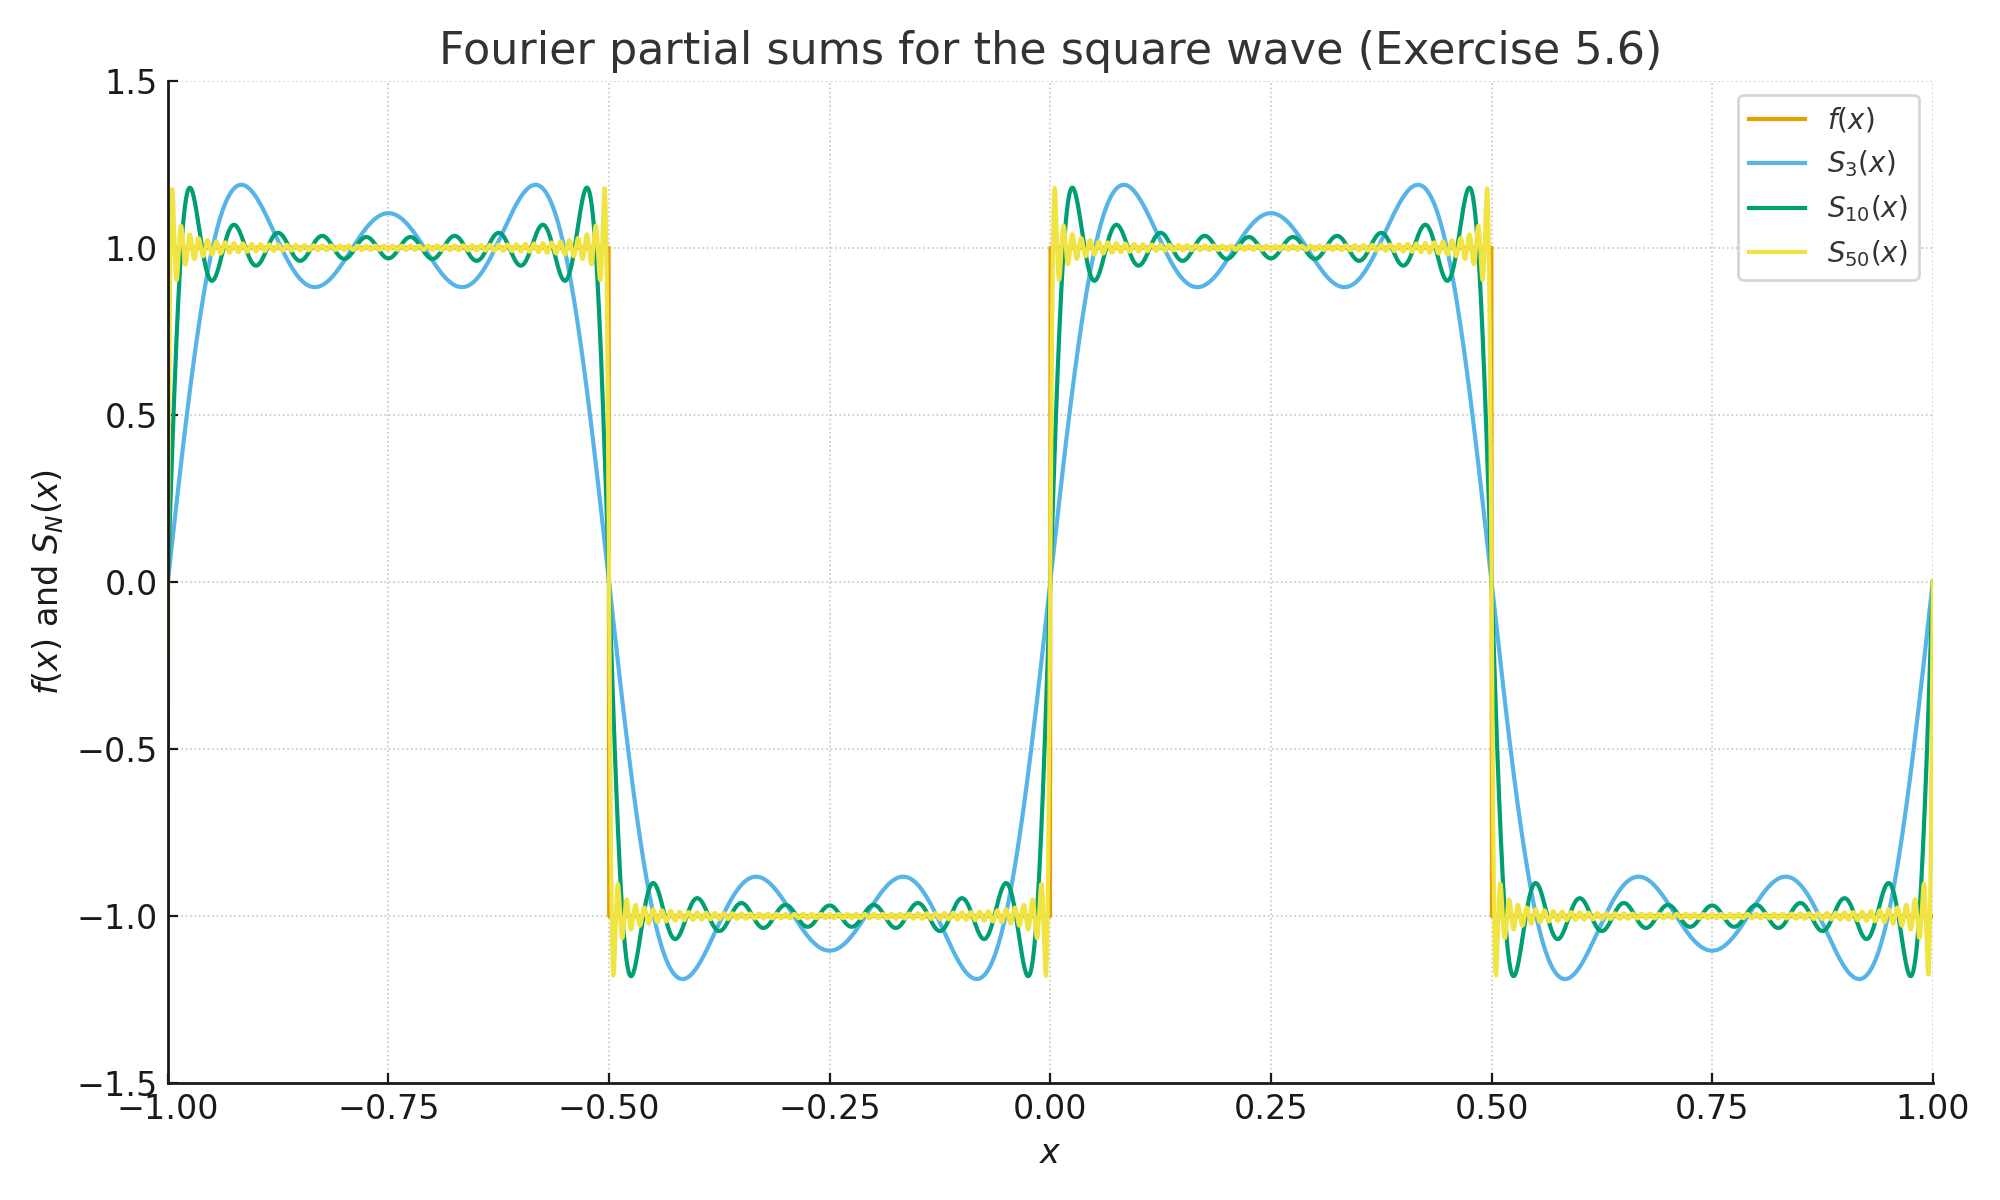
\includegraphics[width=0.90\linewidth]{figures/part02/ex5_6_square_global.png}
  \caption{Global view of the square-wave Fourier partial sums.}
  \label{fig:ex5-6-square-global}
\end{figure}

\begin{figure}[htbp]
  \centering
  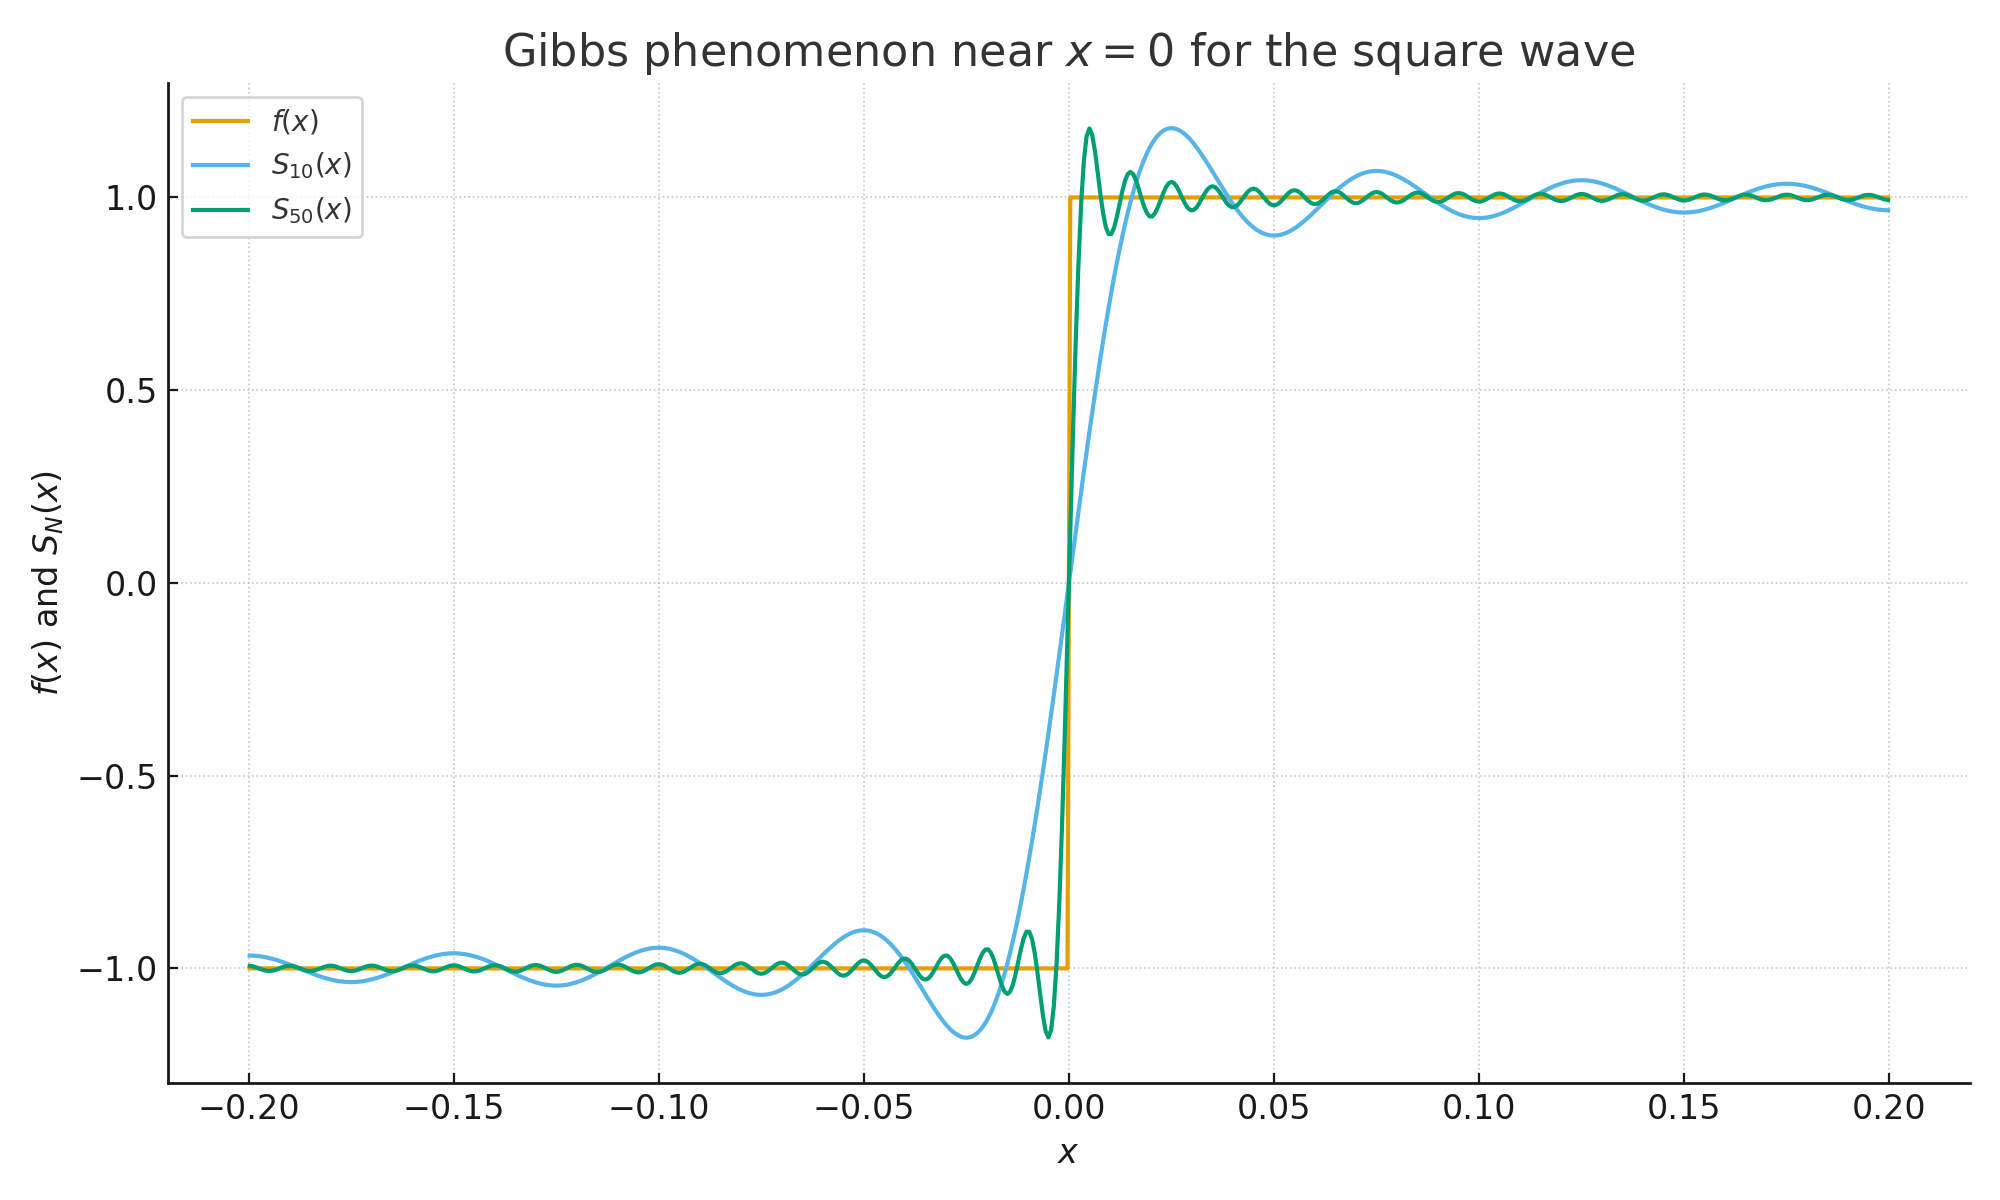
\includegraphics[width=0.88\linewidth]{figures/part02/ex5_6_square_gibbs_zoom.png}
  \caption{Zoom near the jump at $x=0$, showing the persistent Gibbs overshoot.}
  \label{fig:ex5-6-square-gibbs}
\end{figure}

	\clearpage
\end{problem}

\begin{solution}
Up to values assigned at the jump points, which do not affect the Fourier coefficients or
\(L^2\)-class, this is the standard \(1\)-periodic square wave.

Its complex Fourier coefficients are
\[
\widehat f(k)
=
\int_{-1/2}^{1/2}
f(x)e^{-2\pi ikx}\,dx.
\]
Since \(f\) is odd, \(\widehat f(0)=0\). For \(k\neq0\),
\[
\widehat f(k)
=
-\frac{i}{\pi k}\bigl(1-(-1)^k\bigr).
\]
Thus the even coefficients vanish, while for odd \(k\),
\[
\widehat f(k)=\frac{2}{\pi i k}.
\]
Hence
\[
\boxed{
f(x)
=
\frac{1}{\pi i}
\sum_{n\in\mathbb Z}
\frac{2}{2n+1}e^{2\pi i(2n+1)x}
=
\frac4\pi
\sum_{n=0}^{\infty}
\frac{\sin(2\pi(2n+1)x)}{2n+1}
}
\]
in \(L^2_{\mathrm{loc}}(\mathbb R)\).

For the partial sums,
\[
S_N(x)
=
8\sum_{n=0}^{N-1}
\frac{\sin(2\pi(2n+1)x)}
{2\pi(2n+1)}.
\]
Integrating the cosine terms,
\[
\boxed{
S_N(x)
=
8\int_0^x
\sum_{n=0}^{N-1}
\cos(2\pi(2n+1)t)\,dt.
}
\]
Using
\[
\cos(2\pi(2n+1)t)\sin(2\pi t)
=
\frac12
\left[
\sin(2\pi(2n+2)t)-\sin(4\pi nt)
\right],
\]
the sum telescopes to
\[
\sum_{n=0}^{N-1}
\cos(2\pi(2n+1)t)
=
\frac{\sin(4\pi Nt)}{2\sin(2\pi t)}.
\]
Therefore
\[
\boxed{
S_N(x)
=
8\int_0^x
\frac{\sin(4\pi Nt)}{2\sin(2\pi t)}\,dt.
}
\]

Differentiating,
\[
S_N'(x)
=
4\frac{\sin(4\pi Nx)}{\sin(2\pi x)}.
\]
The first positive local maximum occurs at
\[
x_N=\frac1{4N}.
\]
On \(0\le t\le1/(4N)\), the numerator is nonnegative and
\[
\sin(2\pi t)\le2\pi t.
\]
Hence
\[
\begin{aligned}
S_N(x_N)
&\ge
8\int_0^{1/(4N)}
\frac{\sin(4\pi Nt)}{4\pi t}\,dt\\
&=
\frac2\pi
\int_0^\pi
\frac{\sin s}{s}\,ds\\
&\simeq1.17898\ldots.
\end{aligned}
\]
But \(f(x_N)=1\). Thus
\[
\limsup_N\|S_N-f\|_\infty
\ge
1.17898\ldots-1>0.
\]
Therefore
\[
\boxed{
S_N\not\to f\text{ uniformly near the jump}.
}
\]
This persistent overshoot is the Gibbs phenomenon.
\end{solution}


\begin{problem}[CP-II-0408]
\label{prob:cp-ii-0408}
\textbf{Cauchy Sequences and Completeness in the Given Metric.}

\hspace*{1.5em}Pointwise but not uniform (Not Cauchy)

$f_n(x)=x^n$ on $[0,1]$.
Pointwise limit discontinuous, not uniform, not Cauchy in sup norm.

---
\end{problem}

\begin{solution}
Let
\[
f_n(x)=x^n,
\qquad
x\in[0,1].
\]
For \(0\le x<1\),
\[
x^n\to0,
\]
while
\[
f_n(1)=1.
\]
Thus the pointwise limit is
\[
f(x)
=
\begin{cases}
0,&0\le x<1,\\
1,&x=1.
\end{cases}
\]
The limit is discontinuous, whereas every \(f_n\) is continuous, so the convergence cannot be
uniform.

Directly,
\[
\sup_{0\le x<1}|x^n-0|=1
\]
for every \(n\), so
\[
\boxed{f_n\not\to f\text{ uniformly}.}
\]

The sequence is also not Cauchy in the sup norm. Take \(m=2n\) and
\[
x_n=2^{-1/n}.
\]
Then
\[
x_n^n=\frac12,
\qquad
x_n^{2n}=\frac14,
\]
so
\[
\|f_n-f_{2n}\|_\infty
\ge
\frac14
\]
for every \(n\). Hence
\[
\boxed{
(f_n)\text{ is not Cauchy in }\|\cdot\|_\infty.
}
\]
\end{solution}


\begin{problem}[CP-II-0409]
\label{prob:cp-ii-0409}
\textbf{Gaussian.}

\hspace*{1.5em}Let $F(x,y)=e^{-x^2-y^2}$ on $\mathbb{R}$.  Then
\[
\int_{\mathbb{R}}F(x,y)\,dy = \sqrt{\pi}\,e^{-x^2}.
\]
Hence
\[
\int_{\mathbb{R}} \Bigl|\int_{\mathbb{R}}F(x,y)\,dy\Bigr|dx
= \sqrt{\pi}\int_{\mathbb{R}} e^{-x^2}dx
= \pi.
\]
Since $F\ge 0$,
\[
\int_{\mathbb{R}}\int_{\mathbb{R}}|F(x,y)|\,dy\,dx
= \pi.
\]
\end{problem}

\begin{solution}
Let
\[
F(x,y)=e^{-x^2-y^2}.
\]
For fixed \(x\),
\[
\int_{\mathbb R}F(x,y)\,dy
=
e^{-x^2}
\int_{\mathbb R}e^{-y^2}\,dy
=
\sqrt\pi\,e^{-x^2}.
\]
Therefore
\[
\begin{aligned}
\int_{\mathbb R}
\left|
\int_{\mathbb R}F(x,y)\,dy
\right|dx
&=
\sqrt\pi
\int_{\mathbb R}e^{-x^2}\,dx\\
&=
\pi.
\end{aligned}
\]

Since \(F\ge0\),
\[
|F|=F,
\]
and Tonelli gives
\[
\begin{aligned}
\int_{\mathbb R}\int_{\mathbb R}|F(x,y)|\,dy\,dx
&=
\left(
\int_{\mathbb R}e^{-x^2}\,dx
\right)^2\\
&=
\pi.
\end{aligned}
\]
Thus
\[
\boxed{
\int\left|\int F\right|
=
\iint|F|
=
\pi.
}
\]
\end{solution}


\begin{problem}[CP-II-0412]
\label{prob:cp-ii-0412}
\textbf{Lebesgue Decomposition of \(m+\delta_0\).}

\hspace*{1.5em}On $(\mathbb{R},\mathcal B)$ with $\mu=m$ (Lebesgue) and $\nu=m+\delta_0$, we have
		$\nu_a=m$ and $\nu_s=\delta_0$.
\end{problem}

\begin{solution}
Let
\[
\mu=m,
\qquad
\nu=m+\delta_0
\]
on \((\mathbb R,\mathcal B)\).

The Lebesgue-measure part
\[
\nu_a=m
\]
satisfies
\[
\nu_a\ll m.
\]
The Dirac mass is singular with respect to Lebesgue measure because it is concentrated on
\[
\{0\},
\qquad
m(\{0\})=0.
\]
Thus
\[
\nu_s=\delta_0
\]
and
\[
\nu_s\perp m.
\]
Therefore the Lebesgue decomposition is
\[
\boxed{
\nu=\nu_a+\nu_s,
\qquad
\nu_a=m,
\qquad
\nu_s=\delta_0.
}
\]
\end{solution}


\begin{problem}[CP-II-0414]
\label{prob:cp-ii-0414}
\textbf{Surface Measure as a Radon Measure.}

\hspace*{1.5em}Surface measure on a smooth embedded manifold $M\subset\mathbb{R}^n$ is a Radon Borel measure on $M$ (subspace topology).
\end{problem}

\begin{solution}
Let \(M\subset\mathbb R^n\) be a smooth embedded \(d\)-dimensional manifold, equipped with
its subspace topology. Its surface measure is the \(d\)-dimensional volume measure induced
by the smooth charts, equivalently the restriction of \(d\)-dimensional Hausdorff measure to
\(M\) up to the standard normalization.

The space \(M\) is locally compact, Hausdorff, and second countable. In each coordinate
chart, surface measure is represented by
\[
J(u)\,du
\]
with a continuous positive Jacobian factor \(J\). Therefore compact subsets of a chart have
finite surface measure. A compact subset of \(M\) is covered by finitely many such charts, so
surface measure is finite on compact sets.

The chart representation also gives the standard inner and outer regularity of this Borel
measure. Consequently
\[
\boxed{
\text{surface measure on a smooth embedded manifold }M
\text{ is a Radon Borel measure on }M.
}
\]
\end{solution}


\begin{problem}[CP-II-0416]
\label{prob:cp-ii-0416}
\textbf{Continuity of the Given Operator.}

\hspace*{1.5em}Continuity of the Identity Between Two Topologies on the Same Set

Let $\mathrm{id}:(X,\tau)\to (X,\rho)$ be the identity on a fixed set $X$ endowed with (possibly different) topologies $\tau$ and $\rho$. Is $\mathrm{id}$ necessarily continuous?

A map $f:(X,\tau)\to(Y,\sigma)$ is continuous iff $f^{-1}(U)\in\tau$ for all $U\in\sigma$.
For the identity $\mathrm{id}:X\to X$ we have $\mathrm{id}^{-1}(U)=U$ for every $U\subseteq X$.
\end{problem}

\begin{solution}
The identity map
\[
\operatorname{id}:(X,\tau)\to(X,\rho)
\]
is continuous exactly when every \(\rho\)-open set is \(\tau\)-open.

Indeed, continuity means that for every \(U\in\rho\),
\[
\operatorname{id}^{-1}(U)\in\tau.
\]
But the map is the identity, so
\[
\operatorname{id}^{-1}(U)=U.
\]
Hence
\[
\operatorname{id}\text{ is continuous}
\iff
U\in\rho\Longrightarrow U\in\tau
\iff
\rho\subseteq\tau.
\]
Therefore
\[
\boxed{
\operatorname{id}:(X,\tau)\to(X,\rho)
\text{ is continuous iff }\rho\subseteq\tau.
}
\]

Notice the direction: the domain must carry the finer topology. In particular, the
identity is a homeomorphism precisely when both inclusions hold, i.e.
\[
\tau=\rho.
\]
\end{solution}

\begin{problem}[CP-II-0418]
\label{prob:cp-ii-0418}
\textbf{Polynomial Approximation on the Given Compact Set.}

\hspace*{1.5em}For every multi-index $\gamma$ and $1\le p<\infty$,
	\[
	x^\gamma D^\alpha f(x)\in L^p(\mathbb{R}^n),
	\]
	since we may take $N$ large enough to dominate the polynomial
	growth of $x^\gamma$.
\end{problem}

\begin{solution}
Under the rapid-decay hypothesis used in the surrounding Schwartz-space argument, for every
multi-index \(\alpha\) and every \(N\),
\[
|D^\alpha f(x)|
\le
C_{\alpha,N}(1+|x|)^{-N}.
\]
Fix another multi-index \(\gamma\) and \(1\le p<\infty\). Since
\[
|x^\gamma|
\le
C_\gamma(1+|x|)^{|\gamma|},
\]
we have
\[
|x^\gamma D^\alpha f(x)|
\le
C(1+|x|)^{|\gamma|-N}.
\]
Choose \(N\) so large that
\[
p(N-|\gamma|)>n.
\]
Then
\[
|x^\gamma D^\alpha f(x)|^p
\le
C(1+|x|)^{-p(N-|\gamma|)},
\]
and the right-hand side is integrable over \(\mathbb R^n\). Hence
\[
\boxed{
x^\gamma D^\alpha f
\in
L^p(\mathbb R^n)
\qquad
(1\le p<\infty).
}
\]
\end{solution}


\begin{problem}[CP-II-0419]
\label{prob:cp-ii-0419}
\textbf{Fourier Transform of a Regularized Schrödinger Kernel.}

\hspace*{1.5em}Deduce that
		\[
		\widehat{K_\varepsilon^t}(\xi)
		= \left(1+\frac{i4t}{\varepsilon}\right)^{-\tfrac{n}{2}}
		e^{-\, i t|\xi|^2/(1+4it\varepsilon)}.
		\]
\end{problem}

\begin{solution}
The surrounding source regularizes the free Schrödinger kernel by
\[
K_\varepsilon^t(x)
=
e^{-\varepsilon|x|^2}
\frac{1}{(4\pi it)^{n/2}}
e^{\,i|x|^2/(4t)}.
\]
Set
\[
\sigma
=
\varepsilon-\frac{i}{4t},
\qquad
\Re\sigma>0.
\]
Then
\[
K_\varepsilon^t(x)
=
\frac{1}{(4\pi it)^{n/2}}
e^{-\sigma|x|^2}.
\]
Using the Gaussian Fourier integral
\[
\int_{\mathbb R^n}
e^{-\sigma|x|^2-i x\cdot\xi}\,dx
=
\left(\frac{\pi}{\sigma}\right)^{n/2}
e^{-|\xi|^2/(4\sigma)},
\]
we obtain
\[
\begin{aligned}
\widehat{K_\varepsilon^t}(\xi)
&=
(4it\sigma)^{-n/2}
e^{-|\xi|^2/(4\sigma)}\\
&=
(1+4it\varepsilon)^{-n/2}
\exp\left(
-\frac{it|\xi|^2}{1+4it\varepsilon}
\right).
\end{aligned}
\]
Thus
\[
\boxed{
\widehat{K_\varepsilon^t}(\xi)
=
(1+4it\varepsilon)^{-n/2}
e^{-it|\xi|^2/(1+4it\varepsilon)}.
}
\]

The prefactor printed in the migrated source,
\[
\left(1+\frac{4it}{\varepsilon}\right)^{-n/2},
\]
is a typo: it would tend to \(0\), not \(1\), as \(\varepsilon\downarrow0\). The Gaussian
calculation gives the boxed factor above.
\end{solution}


\begin{problem}[CP-II-0420]
\label{prob:cp-ii-0420}
\textbf{Fourier-Analytic Estimates in Sobolev Spaces.}

\hspace*{1.5em}a step function

Let $H(x)=\mathbf{1}_{[1/2,\,1]}(x)$. Then
\[
B_n[H](x)=\sum_{k=\lceil n/2\rceil}^{n}\binom{n}{k}\,x^k(1-x)^{n-k}.
\]
One has
\[
B_n[H](x)\to
\begin{cases}
	0, & x<\tfrac{1}{2},\\[2pt]
	\tfrac12, & x=\tfrac{1}{2},\\[2pt]
	1, & x>\tfrac{1}{2},
\end{cases}
\qquad (n\to\infty).
\]
Hence $B_n[H]\to H$ pointwise at all continuity points of $H$, but not uniformly.
Moreover, for each $1\le p<\infty$,
\[
\|B_n[H]-H\|_{L^p([0,1])}\longrightarrow 0,
\]
so $H$ is approximable by polynomials in $L^p$.

\bigskip

Dropping uniform convergence allows polynomial approximation of discontinuous functions:
 \setlength{\itemsep}{0.6em}
	\par\smallskip\noindent\textbf{(a)}\quad pointwise convergence at continuity points (e.g.\ Bernstein polynomials),
	\par\smallskip\noindent\textbf{(b)}\quad $L^p$-convergence for every $1\le p<\infty$ (polynomials are dense in $L^p$),
	\par\smallskip\noindent\textbf{(c)}\quad often almost-everywhere convergence for suitable subsequences.

Uniform convergence on the whole interval still fails for discontinuous $f$.

Let $(p_n)$ be polynomials on $[0,1]$ converging to $f$ (pointwise, or in $L^p$, $1\le p<\infty$).
If $f$ is not a polynomial, then necessarily $\deg p_n\to\infty$.

\smallskip

\noindent\textbf{Proof (pointwise case).}
Assume $\deg p_n\le m$ for all $n$. Let $\mathcal P_{\le m}$ be the space of polynomials of degree $\le m$.
Choose distinct nodes $x_0,\dots,x_m\in[0,1]$. The evaluation map
\[
T:\mathcal P_{\le m}\to\mathbb{R}^{m+1}, \qquad T(p)=(p(x_0),\dots,p(x_m))
\]
is a linear isomorphism. Since $p_n(x_j)\to f(x_j)$ for each $j$, we have $T(p_n)\to v:=(f(x_0),\dots,f(x_m))$.
Let $p:=T^{-1}(v)\in\mathcal P_{\le m}$. By Lagrange interpolation, for each $x$ there exists a linear functional
$L_x:\mathbb{R}^{m+1}\to\mathbb{R}$ with $p_n(x)=L_x\!\big(T(p_n)\big)$; hence
$p_n(x)\to L_x(v)=p(x)$. Therefore the pointwise limit $f$ equals $p$, a polynomial of degree $\le m$.
Contradiction. Thus $\deg p_n$ cannot be bounded; hence $\deg p_n\to\infty$.


\smallskip

\noindent\textbf{Remark (normed convergences).}
For convergence in any norm (e.g.\ $L^p$), the same conclusion holds since
$\mathcal P_{\le m}$ is finite-dimensional and therefore closed; a limit of $(p_n)$ with $\deg p_n\le m$
must lie in $\mathcal P_{\le m}$.
\end{problem}

\begin{solution}
Let
\[
H(x)=\mathbf1_{[1/2,1]}(x).
\]
Its Bernstein polynomial is
\[
B_n[H](x)
=
\sum_{k=\lceil n/2\rceil}^{n}
\binom nk x^k(1-x)^{n-k}.
\]
This is the probability
\[
\mathbb P(X_n\ge n/2),
\qquad
X_n\sim\operatorname{Bin}(n,x).
\]

If \(x<1/2\), the law of large numbers gives
\[
B_n[H](x)\to0.
\]
If \(x>1/2\),
\[
B_n[H](x)\to1.
\]
At \(x=1/2\), symmetry gives
\[
B_n[H](1/2)\to\frac12.
\]
Hence
\[
\boxed{
B_n[H](x)\to
\begin{cases}
0,&x<1/2,\\
1/2,&x=1/2,\\
1,&x>1/2.
\end{cases}
}
\]
Thus the convergence agrees with \(H\) at every continuity point, but not at the jump.

Uniform convergence to \(H\) is impossible because every Bernstein polynomial is continuous
whereas \(H\) is discontinuous. For \(1\le p<\infty\), however,
\[
0\le B_n[H]\le1
\]
and
\[
B_n[H](x)\to H(x)
\]
for almost every \(x\). Dominated convergence therefore gives
\[
\boxed{
\|B_n[H]-H\|_{L^p([0,1])}\to0.
}
\]

Finally, suppose polynomials \(p_n\) converge pointwise to a nonpolynomial \(f\), or converge
to \(f\) in \(L^p\), and suppose the degrees do not tend to infinity. Then some subsequence
has uniformly bounded degree, say
\[
\deg p_{n_j}\le m.
\]
In the pointwise case, values at \(m+1\) distinct nodes determine a polynomial in the
finite-dimensional space \(\mathcal P_{\le m}\); convergence at those nodes forces the
subsequence to converge to one fixed polynomial, hence \(f\) is that polynomial. In the
\(L^p\) case, \(\mathcal P_{\le m}\) is finite-dimensional and therefore closed, so again
\(f\in\mathcal P_{\le m}\).

Thus, if \(f\) is not a polynomial,
\[
\boxed{\deg p_n\to\infty.}
\]
\end{solution}


\begin{problem}[CP-II-0421]
\label{prob:cp-ii-0421}
\textbf{Gluing Two Intervals by a Quotient Map.}

\hspace*{1.5em}A quotient that bridges two intervals

Let $X=[0,1]\cup[2,3]$ with the subspace topology of $\mathbb{R}$ and define $x\sim y$ iff $x=y$ or $\{x,y\}=\{1,2\}$. Show that $X/\!\sim$ is homeomorphic to $[0,2]$ with the usual topology.
\end{problem}

\begin{solution}
Define $F:X\to[0,2]$ by
	\[
	F(x)=
	\begin{cases}
		x,& x\in[0,1],\\[2pt]
		x-1,& x\in[2,3].
	\end{cases}
	\]
	Then $F$ is continuous (it is continuous on each closed piece, and $F(1)=1=F(2)$), and it is constant on $\sim$-classes (the only nontrivial class is $\{1,2\}$).

	Let $q:X\to X/\!\sim$ be the quotient map. By the universal property of the quotient, there exists a unique continuous $\tilde F:X/\!\sim\to[0,2]$ such that $\tilde F\circ q=F$.

	We show $\tilde F$ is bijective. For $y\in[0,2]$,
	\[
	F^{-1}(\{y\})=
	\begin{cases}
		\{y\},& 0\le y<1,\\
		\{1,2\},& y=1,\\
		\{y+1\},& 1<y\le 2,
	\end{cases}
	\]
	so exactly one equivalence class maps to each $y$. Hence $\tilde F$ is bijective.

	Since $X$ is compact, the quotient $X/\!\sim$ is compact. The space $[0,2]$ is Hausdorff. Therefore a continuous bijection $\tilde F:X/\!\sim\to[0,2]$ is a homeomorphism. Thus $X/\!\sim \cong [0,2]$.
\end{solution}

\begin{problem}[CP-II-0422]
\label{prob:cp-ii-0422}
\textbf{Convolution and Support.}

\begin{lemma}[Mollifiers in $\mathcal{D}'(\mathbb{R}^n)$]
	Let $(\phi_\varepsilon)_{\varepsilon>0}\subset \mathcal{D}(\mathbb{R}^n)$
	be a standard approximate identity as in Theorem~1.13, and let
	$T\in\mathcal{D}'(\mathbb{R}^n)$ be a distribution. Define the
	convolution $\phi_\varepsilon * T$ by
	\[
	\langle \phi_\varepsilon * T, \psi\rangle
	:= \big\langle T, \check{\phi}_\varepsilon * \psi \big\rangle,
	\qquad \psi\in\mathcal{D}(\mathbb{R}^n),
	\]
	where $\check{\phi}_\varepsilon(x):=\phi_\varepsilon(-x)$. Then
	$\phi_\varepsilon * T \in C^\infty(\mathbb{R}^n)$ for every
	$\varepsilon>0$, and
	\[
	\phi_\varepsilon * T \longrightarrow T
	\qquad\text{in }\mathcal{D}'(\mathbb{R}^n)\text{ as }\varepsilon\to0.
	\]
\end{lemma}
\end{problem}

\begin{solution}
Let \((\phi_\varepsilon)\subset\mathcal D(\mathbb R^n)\) be a standard approximate identity
and \(T\in\mathcal D'(\mathbb R^n)\).

For fixed \(\varepsilon>0\), define the ordinary smooth function
\[
u_\varepsilon(x)
=
\langle T,\phi_\varepsilon(x-\cdot)\rangle.
\]
Differentiating with respect to \(x\) is legitimate in the test-function topology, and
\[
D^\alpha u_\varepsilon(x)
=
\langle T,D^\alpha\phi_\varepsilon(x-\cdot)\rangle.
\]
Hence
\[
\boxed{u_\varepsilon\in C^\infty(\mathbb R^n).}
\]

This function represents the distributional convolution in the source:
\[
\langle\phi_\varepsilon*T,\psi\rangle
=
\langle T,\check\phi_\varepsilon*\psi\rangle.
\]

Now let \(\psi\in\mathcal D(\mathbb R^n)\). Standard mollifier theory gives
\[
\check\phi_\varepsilon*\psi
\longrightarrow
\psi
\quad\text{in }\mathcal D.
\]
In particular, for small \(\varepsilon\), all supports remain in one fixed compact set and
all derivatives converge uniformly. Since \(T\) is continuous on \(\mathcal D\),
\[
\langle T,\check\phi_\varepsilon*\psi\rangle
\longrightarrow
\langle T,\psi\rangle.
\]
Therefore
\[
\boxed{
\phi_\varepsilon*T
\to
T
\quad\text{in }\mathcal D'.
}
\]

Thus mollification smooths every distribution and recovers it in the distributional limit.
\end{solution}


\begin{problem}[CP-II-0423]
\label{prob:cp-ii-0423}
\textbf{Weak Convergence and Duality.}

\hfill

		\par\smallskip\noindent\textbf{(a)}\quad Uniform: $f_n(x)=\dfrac{x}{n+x}$ on $[0,1]$; then
		$\sup_{[0,1]}|f_n|=\frac{1}{n+1}\to0$, so $f_n\to0$ uniformly.
		\par\smallskip\noindent\textbf{(b)}\quad Nonuniform: $f_n(x)=x^n$ on $[0,1]$; then $f_n\to f$ pointwise with
		$f=\mathbf 1_{\{1\}}$, but not uniformly, since
		$\sup_{x\in[0,1)}|x^n-0|=1$ for all $n$.
\end{problem}

\begin{solution}
For
\[
f_n(x)=\frac{x}{n+x},
\qquad
x\in[0,1],
\]
the function is nonnegative and increasing in \(x\), so
\[
\|f_n\|_\infty
=
f_n(1)
=
\frac1{n+1}.
\]
Therefore
\[
\boxed{
f_n\to0
\text{ uniformly on }[0,1].
}
\]

By contrast, for
\[
g_n(x)=x^n,
\qquad
x\in[0,1],
\]
the pointwise limit is
\[
g(x)
=
\begin{cases}
0,&0\le x<1,\\
1,&x=1.
\end{cases}
\]
But
\[
\sup_{0\le x<1}x^n=1
\]
for every \(n\). Hence
\[
\boxed{
g_n\to g\text{ pointwise but not uniformly}.
}
\]
\end{solution}


\begin{problem}[CP-II-0425]
\label{prob:cp-ii-0425}
\textbf{Best Denominator $<10$ Approximating $71/49$.}

\hspace*{1.5em}Which rational with denominator less than $10$ best approximates $71/49$?
\end{problem}

\begin{solution}
Let $x=71/49\approx1.4489796$. For each $q=1,\dots,9$ choose $p=\mathrm{round}(qx)$.
The smallest error occurs at $q=9$, $p=13$:
\[
\left|\frac{13}{9}-x\right|\approx 0.00458,
\]
which beats all other denominators $<10$. Therefore the best is $\boxed{13/9}$.

\bigskip
\end{solution}

\begin{problem}[CP-II-0427]
\label{prob:cp-ii-0427}
\textbf{Differentiability from an Increment Estimate.}

\hspace*{1.5em}For the function specified in this exercise, isolate a candidate linear map
\(L\) in the increment
\[
f(a+h)-f(a).
\]
Prove differentiability at \(a\) by showing
\[
\frac{\|f(a+h)-f(a)-Lh\|}{\|h\|}\to0,
\]
and identify \(Df(a)\).
\end{problem}

\begin{solution}
Let
\[
f(x)=x
\qquad(|x|<1/2),
\]
extended periodically with period \(1\).

For \(n=0\),
\[
\widehat f(0)=0.
\]
For \(n\neq0\),
integration by parts gives
\[
\begin{aligned}
\widehat f(n)
&=
\int_{-1/2}^{1/2}
x e^{-2\pi inx}\,dx\\
&=
\frac{i(-1)^n}{2\pi n}.
\end{aligned}
\]
Hence
\[
\boxed{
f(x)
=
\sum_{\substack{n\in\mathbb Z\\n\neq0}}
\frac{i(-1)^n}{2\pi n}
e^{2\pi inx}
}
\]
in \(L^2_{\mathrm{loc}}(\mathbb R)\).

Since \(f\) is odd, write
\[
f(x)
=
\sum_{n=1}^{\infty}
b_n\sin(2\pi nx).
\]
For \(n>0\),
\[
\widehat f(n)=-\frac{i}{2}b_n.
\]
Therefore
\[
b_n
=
2i\,\widehat f(n)
=
\frac{(-1)^{n+1}}{\pi n}.
\]
Thus the real Fourier series is
\[
\boxed{
f(x)
=
\frac1\pi
\sum_{n=1}^{\infty}
\frac{(-1)^{n+1}}{n}
\sin(2\pi nx),
}
\]
with convergence in \(L^2_{\mathrm{loc}}(\mathbb R)\), and pointwise to the midpoint value at
the jump points.

The original formulation briefly states
\[
b_n=\frac{2(-1)^{n+1}}{\pi n},
\]
but its own complex coefficient and its final sine series show that the factor \(2\) there is
a typo. The boxed coefficient is the consistent one. The appended weighted
\(\delta\)-comb figure is unrelated to the sawtooth coefficient calculation.
\end{solution}


\begin{problem}[CP-II-0430]
\label{prob:cp-ii-0430}
\textbf{Differentiability of the Given Nonlinear Map.}

\hspace*{1.5em}Dyadic conditional expectations $P_m f$: step functions constant on $\{I_{m,k}\}$ with $P_m f\to f$ in $L^2$ for $f\in L^2$.
\end{problem}

\begin{solution}
\emph{(a) Orthonormality.} If $(n_1,k_1)\neq(n_2,k_2)$ then either supports are disjoint (integral $0$) or,
when $n_1\neq n_2$, the finer wavelet integrates to $0$ on each child of the coarser support, so the integral vanishes.
Also $\|\psi_{n,k}\|_2^2=\|\psi\|_2^2=1$.

\smallskip
\emph{(b) Density on indicators.} For a finite interval $I$, the dyadic step functions $P_m\mathbf 1_I$ converge to
$\mathbf 1_I$ in $L^2$. Each $P_m\mathbf 1_I$ is a finite combination of $\psi_{n,k}$ (Haar expansion of step functions),
hence $\mathbf 1_I\in\overline{\mathrm{Span}}\{\psi_{n,k}\}$.

\smallskip
\emph{(c) Basis.} Orthonormality from (a) and density from (b) imply $\{\psi_{n,k}\}$ is an orthonormal basis of $L^2(\mathbb{R})$.
\end{solution}

\begin{problem}[CP-II-0431]
\label{prob:cp-ii-0431}
\textbf{Failure of \(L^1\) Convergence to Imply Uniform Convergence.}

\hspace*{1.5em}let $f_n$ be a narrow spike of height $1$ and width $1/n$. Then
	\[
	\|f_n\|_\infty=1 \quad \text{but} \quad \|f_n\|_1=\frac{1}{n}\to 0.
	\]
	Hence convergence in $\|\cdot\|_1$ does not imply convergence in $\|\cdot\|_\infty$.
\end{problem}

\begin{solution}
A concrete example is a rectangular spike on \([0,1]\):
\[
f_n(x)
=
\mathbf1_{[0,1/n]}(x).
\]
Then
\[
\|f_n\|_\infty=1
\]
for every \(n\), while
\[
\|f_n\|_1
=
\int_0^{1/n}1\,dx
=
\frac1n
\longrightarrow0.
\]
Thus
\[
f_n\to0
\quad\text{in }L^1,
\]
but
\[
f_n\not\to0
\quad\text{in }L^\infty.
\]
Hence
\[
\boxed{
L^1\text{-convergence does not imply }L^\infty\text{-convergence}.
}
\]

If continuity of the examples is required, one may replace the rectangle by triangular spikes
of height \(1\) and total area \(1/n\); the same conclusion holds.
\end{solution}


\begin{problem}[CP-II-0432]
\label{prob:cp-ii-0432}
\textbf{Differentiability and the Implicit Function Theorem.}

\hspace*{1.5em}If $(f_n)$ is a sequence of real functions on $[0,1]$ converging uniformly to a function $f$ on $[0,1]$, and if $f_n$ is continuous at $x_n\in[0,1]$ with $x_n\to x$, does it follow that $f$ is continuous at $x$?

  If $(f_n)$ is a sequence of continuous real functions on $[-1,1]$ converging pointwise to a continuous function $f$ on $[-1,1]$, and if the convergence is uniform on $[-r,r]$ for every $r\in(0,1)$, does it follow that the convergence is uniform on $[-1,1]$?

  If $(f_n)$ is a sequence of real functions on the interval $[0,1]$ converging uniformly to a function $f$ on $[0,1]$, and if each $f_n$ is continuous except at countably many points, does it follow that there exists a point at which $f$ is continuous?

  If $(f_n)$ is a sequence of differentiable functions on $[0,1]$ converging uniformly to a function $f$ on $[0,1]$, does it follow that there exists a point at which $f$ is differentiable?

\bigskip

	\par\smallskip\noindent\textbf{(a)}\quad \textbf{Continuity at a point is preserved by uniform limits:} If $f_n\to f$ uniformly on a set $E$ and each $f_n$ is continuous at $x_0\in E$, then $f$ is continuous at $x_0$.
	\par\smallskip\noindent\textbf{(b)}\quad \textbf{Uniform limit of continuous functions is continuous.}
	\par\smallskip\noindent\textbf{(c)}\quad \textbf{Countable union of countable sets is countable.}
	\par\smallskip\noindent\textbf{(d)}\quad \textbf{Local vs global uniformity:} Uniform convergence on $[-r,r]$ for every $r<1$ need not imply uniform convergence on $[-1,1]$.
	\par\smallskip\noindent\textbf{(e)}\quad \textbf{Weierstrass phenomenon:} There exist continuous nowhere differentiable functions that are uniform limits of differentiable functions (e.g., partial sums of the Weierstrass series).

Let
\[
f(x)=\begin{cases}
	0,& x<\tfrac12,\\
	1,& x\ge \tfrac12,
\end{cases}
\qquad \text{and set } f_n=f \text{ for all } n.
\]
Then $f_n\to f$ uniformly. Define $x_n=\tfrac12+\tfrac1n\to x=\tfrac12$. For each $n$, $f_n$ is continuous at $x_n$ (indeed $f$ is continuous at all $x\ne \tfrac12$), but $f$ is discontinuous at $x=\tfrac12$. Hence the asserted implication fails.

For $n\ge1$, define
\[
f_n(x)=
\begin{cases}
	n(1-x),& x\in[1-\tfrac1n,\,1],\\
	0,& x\in[-1,\,1-\tfrac1n),
\end{cases}
\qquad\text{and let } f\equiv 0.
\]
Each $f_n$ is continuous on $[-1,1]$. For any fixed $x\in[-1,1)$, $f_n(x)=0$ for all large $n$, so $f_n(x)\to 0=f(x)$. Also $f_n(1)=0\to 0=f(1)$, hence $f_n\to f$ pointwise and $f$ is continuous. Given any $r\in(0,1)$, if $n>\frac1{1-r}$ then $[1-\frac1n,1]\subset (r,1]$, so $f_n\equiv 0$ on $[-r,r]$; thus convergence is uniform on $[-r,r]$. However,
\[
\sup_{x\in[-1,1]}|f_n(x)-f(x)|=\max_{x\in[-1,1]} f_n(x)=1 \quad\text{for all }n,
\]
so the convergence is not uniform on $[-1,1]$.

Let $D_n$ be the (countable) set of discontinuities of $f_n$ and $D=\bigcup_{n=1}^\infty D_n$, which is countable. Choose $x_0\in[0,1]\setminus D$. Then each $f_n$ is continuous at $x_0$. Since $f_n\to f$ uniformly, the continuity-at-a-point lemma implies $f$ is continuous at $x_0$. Therefore $f$ is continuous at (at least) one point.

Consider the Weierstrass function
\[
W(x)=\sum_{k=0}^\infty a^k\cos(b^k\pi x),
\]
with $0<a<1$, $b\in\mathbb{N}$ odd, and $ab>1$. Let $S_n(x)=\sum_{k=0}^n a^k\cos(b^k\pi x)$. Then each $S_n$ is differentiable on $[0,1]$, and $S_n\to W$ uniformly on $[0,1]$, while $W$ is continuous everywhere and nowhere differentiable. Thus there need not exist any point where $f$ is differentiable.
\end{problem}

\begin{solution}
We answer the four questions in order.

For the first question, the answer is no. Let
\[
f(x)
=
\begin{cases}
0,&x<1/2,\\
1,&x\ge1/2,
\end{cases}
\qquad
f_n=f.
\]
Then \(f_n\to f\) uniformly. Choose
\[
x_n=\frac12+\frac1n\to\frac12.
\]
Each \(f_n\) is continuous at \(x_n\), but \(f\) is discontinuous at \(1/2\). Therefore
continuity at moving points \(x_n\) does not force continuity at their limit:
\[
\boxed{\text{No}.}
\]

For the second question, the answer is also no. Define a continuous triangular spike near
\(1\):
\[
f_n(x)
=
\begin{cases}
0,&x\le1-\frac2n,\\[2mm]
n\left(x-1+\frac2n\right),
&
1-\frac2n\le x\le1-\frac1n,\\[2mm]
n(1-x),
&
1-\frac1n\le x\le1.
\end{cases}
\]
For every fixed \(x<1\), eventually \(f_n(x)=0\), and \(f_n(1)=0\), so
\[
f_n\to0
\]
pointwise. Given any \(r<1\), the support eventually lies in \((r,1]\), so convergence is
uniform on \([-r,r]\). But
\[
\|f_n\|_\infty=1,
\]
so convergence is not uniform on \([-1,1]\):
\[
\boxed{\text{No}.}
\]

For the third question, the answer is yes. Let \(D_n\) be the countable discontinuity set of
\(f_n\). Then
\[
D_*=\bigcup_{n=1}^{\infty}D_n
\]
is countable. Since \([0,1]\) is uncountable, choose
\[
x_0\in[0,1]\setminus D_*.
\]
Every \(f_n\) is continuous at \(x_0\), and a uniform limit of functions all continuous at the
same point is continuous there. Hence
\[
\boxed{f\text{ has at least one point of continuity}.}
\]

For the fourth question, the answer is no. Take a classical Weierstrass function
\[
W(x)
=
\sum_{k=0}^{\infty}
a^k\cos(b^k\pi x),
\]
with, for example,
\[
a=\frac12,
\qquad
b=13.
\]
Then
\[
0<a<1,\qquad b\text{ is odd},\qquad
ab=\frac{13}{2}>1+\frac{3\pi}{2},
\]
so the classical Weierstrass theorem gives a continuous nowhere-differentiable limit. Its
partial sums
\[
S_n(x)
=
\sum_{k=0}^{n}
a^k\cos(b^k\pi x)
\]
are differentiable and converge uniformly by the \(M\)-test. Therefore
\[
\boxed{
\text{a uniform limit of differentiable functions need not be differentiable anywhere}.
}
\]

The migrated source's proposed counterexample for the second question has a jump at
\(x=1-1/n\) despite claiming each \(f_n\) is continuous. The triangular spike above repairs
that example.
\end{solution}


\begin{problem}[CP-II-0437]
\label{prob:cp-ii-0437}
\textbf{Integral Bounds for \(\log(n!)\).}

\hspace*{1.5em}Show that
\[
\int_1^n \log x \, dx \;\leq\; \sum_{k=1}^n \log k \;\leq\; \int_1^n \log x \, dx + \log n.
\]
Deduce that
\[
\log(n!) \sim n\log n - n \quad (n\to\infty).
\]
\end{problem}

\begin{solution}
On each interval $[k,k+1]$, we have
	\[
	\int_k^{k+1} \log x\,dx \;\leq\; \log(k+1).
	\]
	Summing over $k=1,\dots,n-1$ gives
	\[
	\int_1^n \log x\,dx \;\leq\; \sum_{k=2}^n \log k.
	\]
	Adding $\log 1=0$ gives
	\[
	\int_1^n \log x\,dx \;\leq\; \sum_{k=1}^n \log k.
	\]

	Similarly, one checks that
	\[
	\sum_{k=1}^n \log k \;\leq\; \int_1^n \log x\,dx + \log n.
	\]

	Thus
	\[
	n\log n - n + 1 \;\leq\; \log(n!) \;\leq\; n\log n - n + 1 + \log n.
	\]

	Dividing through by $n\log n - n$ and letting $n\to\infty$ shows
	\[
	\frac{\log(n!)}{n\log n - n} \to 1,
	\]
	i.e.
	\[
	\log(n!) \sim n\log n - n.
	\]
\end{solution}

\begin{problem}[CP-II-0439]
\label{prob:cp-ii-0439}
\textbf{Comparison of the Given Function-Space Norms.}

\hspace*{1.5em}On $\mathbb{R}^n$:
	\[
	\|x\|_1=\sum_{i=1}^n |x_i|,\qquad
	\|x\|_2=\Big(\sum_{i=1}^n x_i^2\Big)^{1/2},\qquad
	\|x\|_\infty=\max_{1\le i\le n}|x_i|.
	\]
	There exist constants $a,b>0$ such that
	\[
	\|x\|_\infty \le \|x\|_2 \le \|x\|_1 \le \sqrt{n}\,\|x\|_2.
	\]
	Thus all norms on $\mathbb{R}^n$ are equivalent.
\end{problem}

\begin{solution}
For \(x=(x_1,\ldots,x_n)\in\mathbb R^n\),
\[
\|x\|_1=\sum_i|x_i|,
\qquad
\|x\|_2=\left(\sum_i x_i^2\right)^{1/2},
\qquad
\|x\|_\infty=\max_i|x_i|.
\]
We have
\[
\|x\|_\infty^2
\le
\sum_i|x_i|^2
=
\|x\|_2^2,
\]
so
\[
\|x\|_\infty\le\|x\|_2.
\]
Also
\[
\|x\|_2
\le
\|x\|_1
\]
because
\[
\left(\sum_i|x_i|\right)^2
\ge
\sum_i|x_i|^2.
\]
Finally, Cauchy--Schwarz gives
\[
\|x\|_1
=
\sum_i|x_i|
\le
\sqrt n
\left(\sum_i|x_i|^2\right)^{1/2}
=
\sqrt n\,\|x\|_2.
\]
Thus
\[
\boxed{
\|x\|_\infty
\le
\|x\|_2
\le
\|x\|_1
\le
\sqrt n\,\|x\|_2.
}
\]

These inequalities show that the three standard norms are equivalent. To justify the stronger
statement that every norm on \(\mathbb R^n\) is equivalent, let \(N\) be any norm. Writing
\(x=\sum_i x_i e_i\),
\[
N(x)
\le
\sum_i|x_i|N(e_i)
\le
C\|x\|_2
\]
for some \(C\). Thus \(N\) is Euclidean-continuous. On the compact Euclidean unit sphere,
\(N\) attains a positive minimum \(c>0\). Hence
\[
N(x)
=
\|x\|_2
N\left(\frac{x}{\|x\|_2}\right)
\ge
c\|x\|_2.
\]
Therefore
\[
\boxed{
c\|x\|_2
\le
N(x)
\le
C\|x\|_2,
}
\]
so all norms on \(\mathbb R^n\) are equivalent.
\end{solution}


\begin{problem}[CP-II-0440]
\label{prob:cp-ii-0440}
\textbf{Weak Convergence and Norm Estimates.}

\hspace*{1.5em}Let $(f_n)$ be a sequence of real-valued functions on $[0,1]$ converging uniformly to a function $f$.
For each $n$, let $D_n$ be the set of discontinuities of $f_n$, and let $D$ be the set of discontinuities of $f$.

We show that
\[
D \subseteq \bigcap_{n=1}^{\infty}\ \bigcup_{j=n}^{\infty} D_j
\qquad\text{(the limsup of the sets $D_j$).}
\]
Equivalently, we prove the contrapositive. Suppose $x\notin \limsup D_j$. Then there exists $N$ such that
$x\notin D_j$ for all $j\ge N$. Thus, for all $j\ge N$, the function $f_j$ is continuous at $x$.
Since $f_j \to f$ uniformly on $[0,1]$, the uniform-limit lemma implies that $f$ is continuous at $x$.
Hence $x\notin D$, proving the desired inclusion.

Assume there exists a finite $k$ such that each $f_n$ has at most $k$ discontinuities.
We claim that $f$ has at most $k$ discontinuities.

Suppose, for a contradiction, that $f$ has at least $k+1$ distinct discontinuities $x_1,\dots,x_{k+1}\in[0,1]$.
Let the oscillation of a function $g$ at $x$ be
\[
\omega_g(x)=\lim_{r\downarrow 0}\left(\sup_{|t-x|<r} g(t) - \inf_{|t-x|<r} g(t)\right).
\]
Then $g$ is continuous at $x$ iff $\omega_g(x)=0$. Moreover, if $\|g-h\|_\infty\le \varepsilon$, then
$\omega_g(x)\le\omega_h(x)+2\varepsilon$ and $\omega_h(x)\le\omega_g(x)+2\varepsilon$.

Since $x_i$ is a discontinuity of $f$, we have $\omega_f(x_i)>0$ for each $i$.
Choose $0<\varepsilon<\frac12\min_{1\le i\le k+1}\omega_f(x_i)$.
Because $f_n\to f$ uniformly, there exists $N$ such that $\|f_n-f\|_\infty<\varepsilon$ for all $n\ge N$.
For each $i$ and $n\ge N$,
\[
\omega_{f_n}(x_i)\ \ge\ \omega_f(x_i) - 2\varepsilon\ >\ 0,
\]
so $f_n$ is discontinuous at $x_i$. Hence $f_n$ has at least $k+1$ discontinuities for all $n\ge N$,
contradicting the hypothesis that each $f_n$ has at most $k$ discontinuities.
Therefore $f$ has at most $k$ discontinuities.

(1) From (a) we always have $D \subseteq \limsup D_n$, so if each $D_n$ is finite then $D$ is at most countable.

(2) The conclusion in (b) is stronger: if each $f_n$ has at most $k$ discontinuities for a fixed $k$, then $f$ has at most $k$ discontinuities.

(3) Example (sharpness for $k=1$).

Fix $c\in(0,1)$ and define $f=\mathbf{1}_{[c,1]}$ and $f_n=\mathbf{1}_{[c+1/n,\,1]}$.
Then $f_n\to f$ uniformly, each $f_n$ has exactly one discontinuity, and $f$ has exactly one discontinuity.

Let $k=1$. Fix a point $c\in(0,1)$ and define
\[
f(x) = \mathbf{1}_{[c,1]}(x) =
\begin{cases}
	0, & x < c,\\
	1, & x \ge c,
\end{cases}
\qquad\text{and}\qquad
f_n(x) = \mathbf{1}_{[\,c+1/n,\,1\,]}(x).
\]
Each $f_n$ has exactly one discontinuity (at $x=c+1/n$);
$f_n \to f$ uniformly on $[0,1]$,
and $f$ has exactly one discontinuity (at $x=c$).
This shows that the bound ``$\le k$'' is \emph{sharp}.
\end{problem}

\begin{solution}
Let \(D_n\) be the discontinuity set of \(f_n\), and \(D\) the discontinuity set of the
uniform limit \(f\).

Suppose
\[
x\notin
\limsup_{n\to\infty}D_n
=
\bigcap_{N=1}^{\infty}\bigcup_{j\ge N}D_j.
\]
Then for some \(N\),
\[
x\notin D_j
\qquad(j\ge N).
\]
Thus every function in the tail \((f_j)_{j\ge N}\) is continuous at the same point \(x\).
Since the tail still converges uniformly to \(f\), the usual uniform-limit argument at one
point shows that \(f\) is continuous at \(x\). Hence
\[
\boxed{
D
\subseteq
\limsup_{n\to\infty}D_n.
}
\]

Now assume that every \(f_n\) has at most \(k\) discontinuities. Suppose \(f\) had
\(k+1\) distinct discontinuities
\[
x_1,\ldots,x_{k+1}.
\]
Let \(\omega_g(x)\) denote oscillation at \(x\). Since each \(x_i\) is a discontinuity,
\[
\omega_f(x_i)>0.
\]
Choose
\[
0<\varepsilon
<
\frac12
\min_i\omega_f(x_i).
\]
For all sufficiently large \(n\),
\[
\|f_n-f\|_\infty<\varepsilon.
\]
Oscillation satisfies
\[
|\omega_{f_n}(x)-\omega_f(x)|
\le
2\|f_n-f\|_\infty.
\]
Therefore, for every \(i\),
\[
\omega_{f_n}(x_i)
\ge
\omega_f(x_i)-2\varepsilon
>
0.
\]
So every sufficiently large \(f_n\) is discontinuous at all \(k+1\) points, contradicting the
hypothesis. Hence
\[
\boxed{
\#D\le k.
}
\]

If each \(D_n\) is merely finite with no common cardinal bound, then
\[
\bigcup_{j\ge N}D_j
\]
is countable for every \(N\), so the limsup and therefore \(D\) are at most countable.

The bound \(\#D\le k\) is sharp. For \(k=1\), fix \(c\in(0,1)\) and simply take
\[
f_n=f=\mathbf1_{[c,1]}
\]
for every \(n\). Then the convergence is uniform, every \(f_n\) has exactly one
discontinuity, and so does \(f\).

The moving-jump example printed in the migrated source,
\[
f_n=\mathbf1_{[c+1/n,1]},
\]
does not converge uniformly to \(\mathbf1_{[c,1]}\): the sup-norm difference equals \(1\)
for every \(n\). The constant sequence above supplies the correct sharpness example.
\end{solution}


\begin{problem}[CP-II-0442]
\label{prob:cp-ii-0442}
\textbf{Cauchy Sequences in the Given Normed Space.}

\hspace*{1.5em}Uniform convergence with oscillations (Cauchy)

$f_n(x)=\sin(nx)/n$ on $[0,\pi]$.
Uniform convergence to $f(x)=0$ since $\|f_n-0\|_\infty=1/n \to 0$.
\end{problem}

\begin{solution}
Let
\[
f_n(x)=\frac{\sin(nx)}{n},
\qquad
x\in[0,\pi].
\]
Since
\[
|f_n(x)|\le\frac1n,
\]
we have
\[
\|f_n\|_\infty\le\frac1n\to0.
\]
Thus
\[
\boxed{
f_n\to0
\text{ uniformly on }[0,\pi].
}
\]

In particular the sequence is Cauchy in the sup norm. Indeed,
\[
\|f_n-f_m\|_\infty
\le
\|f_n\|_\infty+\|f_m\|_\infty
\le
\frac1n+\frac1m
\longrightarrow0
\]
as \(m,n\to\infty\).
\end{solution}


\begin{problem}[CP-II-0444]
\label{prob:cp-ii-0444}
\textbf{Uniform Convergence and Interchange of Limits.}

\hspace*{1.5em}Let $L=\sum_{n=1}^\infty 10^{-n!}$ and $r_N=\sum_{n=1}^{N}10^{-n!}=p_N/10^{N!}$.
	Then
	\[
	|L-r_N|=\sum_{n\ge N+1}10^{-n!}
	=10^{-(N+1)!}\Bigl(1+\sum_{n\ge N+2}10^{-(n!-(N+1)!)}\Bigr).
	\]
	For $n\ge N+2$ we have $n!-(N+1)!\ge (N+2)!-(N+1)!=(N+1)N!\ge N!$, hence
	\[
	\sum_{n\ge N+2}10^{-(n!-(N+1)!)}\le \sum_{k=1}^\infty (10^{-N!})^{k}
	=\frac{10^{-N!}}{1-10^{-N!}}\le \frac{1}{9}.
	\]
	Therefore
	\[
	\boxed{\ |L-r_N|< \frac{10}{9}\,10^{-(N+1)!}\ }.
	\]
	Fix $m\in\mathbb N$ and choose $N\ge m$. Since $((N+1)-m)N!\ge N!\ge1$,
	\[
	\frac{10}{9}\,10^{-(N+1)!}
	=\frac{10}{9}\,10^{-((N+1)-m)N!}\cdot 10^{-mN!}\le 10^{-mN!}
	=\frac{1}{(10^{N!})^{\,m}}.
	\]
	Thus for $q_N=10^{N!}$ we obtain
	\[
	\Bigl|L-\frac{p_N}{q_N}\Bigr|<\frac{1}{q_N^{\,m}}
	\quad\text{for all }N\ge m.
	\]
	Since this holds for every $m$ and infinitely many $N$, $L$ is a Liouville number and hence transcendental.
\end{problem}

\begin{solution}
Let
\[
L=\sum_{n=1}^{\infty}10^{-n!},
\qquad
r_N=\sum_{n=1}^{N}10^{-n!}
=\frac{p_N}{10^{N!}}.
\]
Then
\[
L-r_N
=
10^{-(N+1)!}
\left(
1+
\sum_{n\ge N+2}
10^{-(n!-(N+1)!)}
\right).
\]
For the \(k\)-th term after \(N+1\), the exponent difference is at least \(kN!\), so
\[
\sum_{n\ge N+2}
10^{-(n!-(N+1)!)}
\le
\sum_{k=1}^{\infty}
(10^{-N!})^k
=
\frac{10^{-N!}}{1-10^{-N!}}
\le
\frac19.
\]
Hence
\[
\boxed{
0<L-r_N
<
\frac{10}{9}\,10^{-(N+1)!}.
}
\]

Fix \(m\in\mathbb N\) and choose \(N\ge m\). Since
\[
(N+1)!
=
(N+1)N!,
\]
we have
\[
\begin{aligned}
\frac{10}{9}10^{-(N+1)!}
&=
\frac{10}{9}
10^{-((N+1)-m)N!}
10^{-mN!}\\
&\le
10^{-mN!}.
\end{aligned}
\]
With
\[
q_N=10^{N!},
\]
this gives
\[
\left|
L-\frac{p_N}{q_N}
\right|
<
\frac1{q_N^m}.
\]
For every fixed \(m\), this holds for infinitely many \(N\). If the fraction is reduced,
its denominator only decreases, so the Liouville estimate remains valid. Thus
\[
\boxed{
L\text{ is a Liouville number and therefore transcendental}.
}
\]
\end{solution}


\begin{problem}[CP-II-0446]
\label{prob:cp-ii-0446}
\textbf{Dirichlet energy and eigenvalues.}

\hspace*{1.5em}Let $\Omega\subset\mathbb{R}^n$ be open and bounded. For $u\in H_0^1(\Omega)$
define the Dirichlet energy
\[
E[u] = \int_\Omega |Du(x)|^2\,dx.
\]
\end{problem}

\begin{solution}
\par\medskip\noindent\textbf{(a)}\quad  Since $u_i\rightharpoonup u$ in $H_0^1(\Omega)$, one has
$Du_i\rightharpoonup Du$ in $L^2(\Omega;\mathbb{R}^n)$. The map
$L^2\ni f\mapsto\|f\|_{L^2}^2$ is convex and weakly lower semicontinuous,
hence
\[
E[u]=\|Du\|_{L^2}^2\le
\liminf_{i\to\infty}\|Du_i\|_{L^2}^2
=\liminf_{i\to\infty}E[u_i].
\]

\par\medskip\noindent\textbf{(b)}\quad  By definition of $\lambda_1$ there exists a sequence
$(u_k)\subset H_0^1(\Omega)$ with
\[
\|u_k\|_{L^2}=1,\qquad E[u_k]\to\lambda_1.
\]
Then
\[
\|u_k\|_{H^1}^2=\|u_k\|_{L^2}^2+\|Du_k\|_{L^2}^2
=1+E[u_k],
\]
so $(u_k)$ is bounded in $H_0^1(\Omega)$. By weak compactness and the
Rellich--Kondrachov theorem there is a subsequence (denoted again $u_k$)
and $w_1\in H_0^1(\Omega)$ such that
\[
u_k\rightharpoonup w_1\quad\text{in }H_0^1(\Omega),\qquad
u_k\to w_1\quad\text{in }L^2(\Omega).
\]
In particular
\[
\|w_1\|_{L^2}=\lim_{k\to\infty}\|u_k\|_{L^2}=1.
\]
By part (a),
\[
E[w_1]\le\liminf_{k\to\infty}E[u_k]=\lambda_1.
\]
Since $\lambda_1$ is the infimum of $\mathcal{E}_1$, we also have
$\lambda_1\le E[w_1]$. Thus $E[w_1]=\lambda_1$.

If $\lambda_1=0$, then $E[w_1]=0$ and hence $Dw_1=0$ a.e., so $w_1$ is
constant. Because $w_1\in H_0^1(\Omega)$ its trace on $\partial\Omega$ is
zero, hence $w_1\equiv 0$, contradicting $\|w_1\|_{L^2}=1$. Therefore
$\lambda_1>0$.

\par\medskip\noindent\textbf{(c)}\quad  Let $u\in H_0^1(\Omega)$, $u\neq 0$, and set
$v=u/\|u\|_{L^2}$. Then $\|v\|_{L^2}=1$ and by definition of $\lambda_1$
\[
\lambda_1\le E[v]
=\int_\Omega|Dv|^2
=\frac{1}{\|u\|_{L^2}^2}\int_\Omega |Du|^2.
\]
Hence
\[
\lambda_1\|u\|_{L^2}^2\le\int_\Omega |Du|^2.
\]
For $u=0$ the inequality holds trivially. If $u=w_1$, then
$E[u]=\lambda_1\|u\|_{L^2}^2$ and equality holds.

\par\medskip\noindent\textbf{(d)}\quad  Consider the functional
\[
J(u):=E[u]-\lambda_1\|u\|_{L^2}^2.
\]
Since $w_1$ minimises $E$ under the constraint $\|u\|_{L^2}=1$, there is a
Lagrange multiplier $\lambda_1$ and $w_1$ is a stationary point of $J$.
For $\varphi\in C_c^\infty(\Omega)$ one has
\[
0 = \left.\frac{d}{dt}J(w_1+t\varphi)\right|_{t=0}
=2\int_\Omega Dw_1\cdot D\varphi
-2\lambda_1\int_\Omega w_1\varphi.
\]
Thus
\[
\int_\Omega Dw_1\cdot D\varphi
=\lambda_1\int_\Omega w_1\varphi,
\qquad\forall\,\varphi\in C_c^\infty(\Omega).
\]
By the definition of the distributional Laplacian,
\[
\langle -\Delta w_1,\varphi\rangle
=\int_\Omega Dw_1\cdot D\varphi,
\]
so
\[
\langle -\Delta w_1,\varphi\rangle
=\lambda_1\int_\Omega w_1\varphi
=\langle \lambda_1 w_1,\varphi\rangle
\]
for all $\varphi\in C_c^\infty(\Omega)$, which means
\[
-\Delta w_1=\lambda_1 w_1 \quad\text{in }\mathcal{D}'(\Omega).
\]

\par\medskip\noindent\textbf{(e)}\quad  Let $\chi\in C_c^\infty(\Omega)$ and put $v=\chi w_1$,
extended by zero to $\mathbb{R}^n$. Then
\[
-\Delta v = -\Delta(\chi w_1)
= -\chi\Delta w_1 - 2\nabla\chi\cdot\nabla w_1 - w_1\Delta\chi.
\]
Using $-\Delta w_1=\lambda_1 w_1$ we obtain
\[
-\Delta v + v
= \chi(\lambda_1+1)w_1 - 2\nabla\chi\cdot\nabla w_1 - w_1\Delta\chi
=:f.
\]
Since $w_1\in H_0^1(\Omega)$ and $\chi,\nabla\chi,\Delta\chi$ are smooth with
compact support, we have $f\in L^2(\mathbb{R}^n)$.

Taking Fourier transforms on $\mathbb{R}^n$, the equation
$-\Delta v + v = f$ becomes
\[
(|\xi|^2+1)\widehat{v}(\xi)=\widehat{f}(\xi).
\]
Thus
\[
\widehat{v}(\xi)=\frac{\widehat{f}(\xi)}{|\xi|^2+1}
\]
and
\[
\int_{\mathbb{R}^n}(1+|\xi|^2)^2|\widehat{v}(\xi)|^2\,d\xi
\le\int_{\mathbb{R}^n}|\widehat{f}(\xi)|^2\,d\xi<\infty,
\]
so $v\in H^2(\mathbb{R}^n)$. Since $\chi$ was arbitrary, this shows that
$w_1\in H^2_{\mathrm{loc}}(\Omega)$. Iterating the argument gives
$w_1\in H^k_{\mathrm{loc}}(\Omega)$ for all $k$, and therefore
$w_1\in C^\infty(\Omega)$ by Sobolev embedding. Together with
$w_1\in H_0^1(\Omega)$ we obtain
\[
w_1\in H_0^1(\Omega)\cap C^\infty(\Omega).
\]

\par\medskip\noindent\textbf{(f)}\quad  Define
\[
\mathcal{E}_2
=\{E[u]:u\in H_0^1(\Omega),\ \|u\|_{L^2}=1,\ (u,w_1)_{L^2}=0\},
\qquad
\lambda_2:=\inf\mathcal{E}_2.
\]
Choose a sequence $(u_k)$ with $\|u_k\|_{L^2}=1$,
$(u_k,w_1)_{L^2}=0$ and $E[u_k]\to\lambda_2$. As in (b),
$(u_k)$ is bounded in $H_0^1(\Omega)$, so up to a subsequence
\[
u_k\rightharpoonup w_2\text{ in }H_0^1(\Omega),
\qquad
u_k\to w_2\text{ in }L^2(\Omega).
\]
Then
\[
\|w_2\|_{L^2}=1,\qquad (w_2,w_1)_{L^2}=0,
\]
and by part (a),
\[
E[w_2]\le\liminf_{k\to\infty}E[u_k]=\lambda_2.
\]
Since $\lambda_2$ is the infimum over the same constraint set,
we must have $E[w_2]=\lambda_2$.

For every $u\in H_0^1(\Omega)$ with $u\neq 0$ we have
\[
\frac{E[u]}{\|u\|_{L^2}^2}\ge\lambda_1,
\]
so in particular $\lambda_2\ge\lambda_1$.

To derive the Euler--Lagrange equation, consider
\[
J(u)=E[u]-\lambda_2\|u\|_{L^2}^2-\mu (u,w_1)_{L^2},
\]
with Lagrange multipliers $\lambda_2,\mu$. Stationarity of $J$ at $w_2$
in the direction $\varphi\in C_c^\infty(\Omega)$ gives
\[
\int_\Omega Dw_2\cdot D\varphi
=\lambda_2\int_\Omega w_2\varphi + \frac{\mu}{2}\int_\Omega w_1\varphi.
\]
Choosing $\varphi=w_1$ shows $\mu=0$ (using $(w_2,w_1)_{L^2}=0$), and thus
\[
\int_\Omega Dw_2\cdot D\varphi
=\lambda_2\int_\Omega w_2\varphi,\qquad
\forall\,\varphi\in C_c^\infty(\Omega),
\]
which means
\[
-\Delta w_2=\lambda_2 w_2\quad\text{in }\mathcal{D}'(\Omega).
\]
The same localisation and regularity argument as in (e) shows that
$w_2\in C^\infty(\Omega)$, so $w_2\in H_0^1(\Omega)\cap C^\infty(\Omega)$.
\end{solution}

\begin{problem}[CP-II-0447]
\label{prob:cp-ii-0447}
\textbf{Polynomial Approximation and Uniform Convergence.}

\hspace*{1.5em}Let
\[
K=\{z\in\mathbb C:|z|=1,\ \Re z\ge0\}
\]
be the closed right semicircle.

Show that there exists a sequence of polynomials \(p_n\) such that
\[
p_n(z)\longrightarrow\frac1z
\]
uniformly on \(K\).

In particular, show that the polynomials may be chosen so that
\[
\sup_{z\in K}
\left|p_n(z)-\frac1z\right|<\frac1n.
\]
\end{problem}

\begin{solution}
Consider polynomial approximation of
\[
\frac1z
\]
on the compact right semicircle
\[
K=\{z:|z|=1,\ \Re z\ge0\}.
\]
Since \(K\) has empty interior, \(\mathbb C\setminus K\) is connected, and \(0\notin K\),
the function \(1/z\) is continuous on \(K\) and holomorphic on a neighborhood of \(K\).

Mergelyan's theorem therefore gives, for every \(n\), a polynomial \(p_n\) satisfying
\[
\sup_{z\in K}
\left|
p_n(z)-\frac1z
\right|
<
\frac1n.
\]
Hence
\[
\boxed{
p_n\to\frac1z
\quad\text{uniformly on }K.
}
\]

The source mentions Faber-polynomial and discrete least-squares constructions. Mergelyan's
theorem guarantees existence of uniformly approximating polynomials, but by itself it does
not imply that an arbitrary discrete least-squares scheme converges uniformly; such a
numerical construction needs its own stability and sampling hypotheses.
\end{solution}


\begin{problem}[CP-II-0448]
\label{prob:cp-ii-0448}
\textbf{Function-Space Analysis.}

\hspace*{1.5em}More conceptually: the functions $x \mapsto x^p/p$ and
	$y \mapsto y^q/q$ are Legendre transforms of each other.
	Young's inequality expresses this duality.
\end{problem}

\begin{solution}
Let
\[
1<p<\infty,
\qquad
\frac1p+\frac1q=1,
\]
and define
\[
\Phi(x)=\frac{x^p}{p},
\qquad x\ge0.
\]
Its convex conjugate is
\[
\Phi^*(y)
=
\sup_{x\ge0}
\left(
xy-\frac{x^p}{p}
\right).
\]
The maximizing point satisfies
\[
y=x^{p-1},
\]
so
\[
x=y^{q-1}.
\]
Substitution gives
\[
\Phi^*(y)=\frac{y^q}{q}.
\]
Thus the two functions
\[
x\mapsto\frac{x^p}{p},
\qquad
y\mapsto\frac{y^q}{q}
\]
are Legendre transforms of one another.

Fenchel--Young says
\[
xy\le\Phi(x)+\Phi^*(y),
\]
hence
\[
\boxed{
xy\le\frac{x^p}{p}+\frac{y^q}{q}.
}
\]
Therefore Young's inequality is precisely the pointwise inequality associated with this
Legendre duality.
\end{solution}


\begin{problem}[CP-II-0449]
\label{prob:cp-ii-0449}
\textbf{Norm $\Rightarrow$ weak $\Rightarrow$ weak-* on $X'$.}

\hspace*{1.5em}Let $X$ be a Banach space and let $(\Lambda_k)\subset X'$. Show that
	\[
	\|\Lambda_k-\Lambda\|\to0 \ \Longrightarrow\ \Lambda_k \xrightarrow{\;\sigma(X',X'')\;} \Lambda
	\ \Longrightarrow\ \Lambda_k \xrightarrow{\;\sigma(X',X)\;} \Lambda .
	\]
\end{problem}

\begin{solution}
If $\|\Lambda_k-\Lambda\|\to0$ then, for any $\Phi\in X''$,
	\[
	|\Phi(\Lambda_k-\Lambda)| \le \|\Phi\|\,\|\Lambda_k-\Lambda\| \to 0,
	\]
	so $\Lambda_k\to\Lambda$ in the weak topology $\sigma(X',X'')$.
	If $\Lambda_k\to\Lambda$ in $\sigma(X',X'')$, then for each $x\in X$,
	identify $Jx\in X''$ by $Jx(\Gamma)=\Gamma(x)$. Hence
	\[
	\Lambda_k(x)=Jx(\Lambda_k) \longrightarrow Jx(\Lambda)=\Lambda(x).
	\]
	Thus $\Lambda_k\to\Lambda$ in the weak-*\ topology $\sigma(X',X)$.
\end{solution}

\begin{problem}[CP-II-0450]
\label{prob:cp-ii-0450}
\textbf{Shrinking supports.}
		In $\mathbb R^{n}$, set $f_j := |B_{1/j}|^{-1/p}\,\mathbf 1_{B_{1/j}}$. Then $\|f_j\|_p=1$ and
		$f_j\rightharpoonup 0$ in $L^{p}$; indeed $\int f_j h \to 0$ for $h\in C_c^\infty$, then extend to $L^{p'}$.
\end{problem}

\begin{solution}
Let
\[
f_j
=
|B_{1/j}|^{-1/p}\mathbf1_{B_{1/j}}
\]
in \(\mathbb R^n\). Then
\[
\|f_j\|_p^p
=
|B_{1/j}|^{-1}
|B_{1/j}|
=
1,
\]
so
\[
\boxed{\|f_j\|_p=1.}
\]

Assume
\[
1<p<\infty
\]
and let \(p'\) be the conjugate exponent. For \(h\in L^{p'}\),
\[
\begin{aligned}
\left|
\int f_jh
\right|
&\le
|B_{1/j}|^{-1/p}
\|h\|_{L^{p'}(B_{1/j})}
\|\mathbf1_{B_{1/j}}\|_{L^p}\\
&=
\|h\|_{L^{p'}(B_{1/j})}.
\end{aligned}
\]
Since \(p'<\infty\), absolute continuity of the \(L^{p'}\)-integral gives
\[
\|h\|_{L^{p'}(B_{1/j})}\to0.
\]
Therefore
\[
\boxed{
f_j\rightharpoonup0
\quad\text{in }L^p(\mathbb R^n),
\qquad
1<p<\infty.
}
\]

The endpoint \(p=1\) is different. Then
\[
f_j=|B_{1/j}|^{-1}\mathbf1_{B_{1/j}},
\]
and pairing with the constant function \(1\in L^\infty\) gives
\[
\int f_j=1.
\]
Hence
\[
\boxed{
f_j\not\rightharpoonup0
\quad\text{in }L^1.
}
\]
So the weak-convergence claim in the source requires \(1<p<\infty\).
\end{solution}


\begin{problem}[CP-II-0451]
\label{prob:cp-ii-0451}
\textbf{Establish the following lower-semicontinuity principles.}

\par\hspace*{1.5em}\textbf{(a)}\quad
If \(u_n\to u\) in \(L^1(\Omega)\), prove that
\[
\operatorname{TV}(u)
\le
\liminf_{n\to\infty}\operatorname{TV}(u_n).
\]

\par\noindent\textbf{(b)}\quad
If \(x_n\rightharpoonup x\) in a Hilbert space, prove
\[
\|x\|\le\liminf_{n\to\infty}\|x_n\|.
\]
Show moreover that if
\[
\|x_n\|\to\|x\|,
\]
then \(x_n\to x\) strongly.

\par\noindent\textbf{(c)}\quad
Give examples showing that weak lower semicontinuity of the norm may
be strict.

\par\noindent\textbf{(d)}\quad
For the Dirichlet energy
\[
E(u)=\int_\Omega|\nabla u|^2\,dx,
\]
prove weak lower semicontinuity in \(H^1\), give a strict example, and
explain how weak lower semicontinuity enters the direct method for
minimizing \(E\) with fixed boundary data.
\end{problem}

\begin{solution}
We first prove lower semicontinuity of total variation. For \(u\in L^1(\Omega)\),
\[
\operatorname{TV}(u)
=
\sup\left\{
\int_\Omega u\,\operatorname{div}\varphi\,dx:
\varphi\in C_c^1(\Omega;\mathbb R^n),\
\|\varphi\|_\infty\le1
\right\}.
\]
If
\[
u_n\to u
\quad\text{in }L^1(\Omega),
\]
then for every admissible \(\varphi\),
\[
\int u_n\operatorname{div}\varphi
\longrightarrow
\int u\operatorname{div}\varphi.
\]
Therefore
\[
\int u\operatorname{div}\varphi
\le
\liminf_n\operatorname{TV}(u_n).
\]
Taking the supremum over \(\varphi\),
\[
\boxed{
\operatorname{TV}(u)
\le
\liminf_n\operatorname{TV}(u_n).
}
\]

In a Hilbert space, if
\[
x_n\rightharpoonup x,
\]
then the norm is weakly lower semicontinuous:
\[
\|x\|
\le
\liminf_n\|x_n\|.
\]
If in addition
\[
\|x_n\|\to\|x\|,
\]
then
\[
\begin{aligned}
\|x_n-x\|^2
&=
\|x_n\|^2+\|x\|^2
-2\operatorname{Re}\langle x_n,x\rangle\\
&\longrightarrow0.
\end{aligned}
\]
Thus
\[
\boxed{
x_n\rightharpoonup x
\text{ and }
\|x_n\|\to\|x\|
\Longrightarrow
x_n\to x
\text{ strongly}.
}
\]

For strict weak lower semicontinuity in \(L^p(\mathbb R)\), the moving bumps
\[
f_n=\mathbf1_{(n,n+1)}
\]
satisfy
\[
f_n\rightharpoonup0
\quad\text{for }1<p<\infty,
\qquad
\|f_n\|_p=1.
\]
Thus
\[
0=\|0\|_p
<
\liminf_n\|f_n\|_p.
\]
This statement is false at \(p=1\), as the source itself later notes: pairing with a suitable
bounded function can prevent weak convergence.

The oscillatory \(L^2\)-example
\[
f_n(x)=\sin(2\pi nx)
\]
on \([0,1]\) satisfies
\[
f_n\rightharpoonup0,
\qquad
\|f_n\|_2=\frac1{\sqrt2},
\]
so the weak l.s.c. inequality is again strict.

For the Dirichlet energy
\[
E(u)=\int_\Omega|\nabla u|^2\,dx,
\]
weak \(H^1\)-convergence implies weak \(L^2\)-convergence of gradients, hence
\[
\boxed{
E(u)\le\liminf_nE(u_n).
}
\]
A correct strict example on \((0,1)\) is
\[
u_n(x)
=
\frac{\sin(2\pi nx)}{2\pi n}.
\]
Then
\[
u_n\rightharpoonup0
\quad\text{in }H_0^1(0,1),
\]
because \(u_n\to0\) strongly in \(L^2\) and
\[
u_n'(x)=\cos(2\pi nx)\rightharpoonup0
\quad\text{in }L^2,
\]
while
\[
E(u_n)
=
\int_0^1\cos^2(2\pi nx)\,dx
=
\frac12.
\]
Thus
\[
E(0)=0<\liminf_nE(u_n).
\]

The source's unscaled choice \(u_n=\sin(2\pi nx)\) is not weakly convergent in \(H^1\),
because its \(H^1\)-norm tends to infinity and every weakly convergent sequence is bounded.

Finally, for the direct method with fixed boundary data, choose one extension
\(G\in H^1(\Omega)\) of the boundary datum. A minimizing sequence \(u_k\) satisfies
\(u_k-G\in H_0^1(\Omega)\). Bounded energy plus Poincare's inequality gives boundedness in
\(H^1\). Reflexivity gives a weakly convergent subsequence, the trace condition is weakly
closed, and weak l.s.c. yields a minimizer.
\end{solution}


\begin{problem}[CP-II-0452]
\label{prob:cp-ii-0452}
\textbf{Uniform Continuity and Compactness.}

\hspace*{1.5em}For the continuous function and domain specified in this exercise, determine
whether uniform continuity holds. Use compactness when available; otherwise
either produce a global modulus/Lipschitz estimate or construct pairs of
nearby points showing failure of uniform continuity.
\end{problem}

\begin{solution}
If
\[
f_n\to f,
\qquad
g_n\to g
\]
uniformly on \(E\), then
\[
\begin{aligned}
\|(f_n+g_n)-(f+g)\|_\infty
&\le
\|f_n-f\|_\infty
+
\|g_n-g\|_\infty\\
&\to0.
\end{aligned}
\]
Thus
\[
\boxed{f_n+g_n\to f+g\text{ uniformly}.}
\]

Products need not behave this way on an unbounded domain. Take
\[
E=\mathbb R,
\qquad
f_n(x)=\frac1n,
\qquad
f(x)=0,
\qquad
g_n(x)=g(x)=x.
\]
Then \(f_n\to0\) and \(g_n\to g\) uniformly, but
\[
f_ng_n(x)=\frac xn,
\]
so
\[
\sup_{x\in\mathbb R}\left|\frac xn\right|=\infty.
\]
Hence
\[
\boxed{
f_ng_n\not\to fg
\text{ uniformly in general}.
}
\]

Now suppose \(f\) and \(g\) are bounded:
\[
|f|\le M,
\qquad
|g|\le L.
\]
Uniform convergence implies that \(g_n\) is eventually uniformly bounded, say
\[
\|g_n\|_\infty\le L+1.
\]
Then
\[
\begin{aligned}
\|f_ng_n-fg\|_\infty
&\le
\|(f_n-f)g_n\|_\infty
+
\|f(g_n-g)\|_\infty\\
&\le
(L+1)\|f_n-f\|_\infty
+
M\|g_n-g\|_\infty
\to0.
\end{aligned}
\]
Therefore
\[
\boxed{
\text{if the limits are bounded, then }
f_ng_n\to fg
\text{ uniformly}.
}
\]
\end{solution}


\begin{problem}[CP-II-0455]
\label{prob:cp-ii-0455}
\textbf{Continuity on Subspaces and Relative Topology.}

\hspace*{1.5em}(Trace theorem on a hyperplane)

Assume $s>\tfrac12$ and suppose $u\in\mathcal S(\mathbb R^n)$.
Write $x=(x',x_n)\in\mathbb R^{n-1}\times\mathbb R$ and define the trace
\[
Tu(x') := u(x',0),\qquad x'\in\mathbb R^{n-1}.
\]

Show that for each $\xi'\in\mathbb R^{n-1}$ one has
\[
\widehat{Tu}(\xi') = \frac{1}{2\pi}\int_{\mathbb R}\widehat u(\xi',\xi_n)\,d\xi_n.
\]

Deduce that
\[
\bigl|\widehat{Tu}(\xi')\bigr|^2
\;\le\;
\frac{1}{(2\pi)^2}
\left(\int_{\mathbb R} (1+|\xi|^2)^s\,|\widehat u(\xi',\xi_n)|^2\,d\xi_n\right)
\left(\int_{\mathbb R}\frac{d\xi_n}{(1+|\xi|^2)^s}\right),
\]
where $\xi=(\xi',\xi_n)$.

By changing variables in the second integral above to
$\xi_n = t\sqrt{1+|\xi'|^2}$, show that there exists a constant $C(s)>0$
such that
\[
\|Tu\|_{H^{s-\frac12}(\mathbb R^{n-1})}
\;\le\; C(s)\,\|u\|_{H^s(\mathbb R^n)}.
\]

Conclude that $T$ extends uniquely by density to a bounded linear operator
\[
T:H^s(\mathbb R^n)\longrightarrow H^{s-\frac12}(\mathbb R^{n-1}),
\qquad s>\tfrac12.
\]

Suppose $\nu\in\mathcal S(\mathbb R^{n-1})$ and let $\phi\in C_c^\infty(\mathbb R)$ satisfy
\[
\int_{\mathbb R}\phi(t)\,dt = \sqrt{2\pi}.
\]
Define $u$ through its Fourier transform by
\[
\widehat u(\xi',\xi_n)
:= \frac{\widehat\nu(\xi')}{\sqrt{1+|\xi'|^2}}\,
\phi\!\left(\frac{\xi_n}{\sqrt{1+|\xi'|^2}}\right).
\]
Show that there exists a constant $C>0$ such that
\[
\|u\|_{H^s(\mathbb R^n)} \le C\,\|\nu\|_{H^{s-\frac12}(\mathbb R^{n-1})}.
\]
Compute $Tu$ and verify that $Tu=\nu$. Conclude that
\[
T:H^s(\mathbb R^n)\longrightarrow H^{s-\frac12}(\mathbb R^{n-1})
\]
is surjective and hence an isomorphism onto $H^{s-\frac12}(\mathbb R^{n-1})$.

\bigskip

For $s>\tfrac12$ the trace operator
\[
T:H^s(\mathbb R^n)\to H^{s-\frac12}(\mathbb R^{n-1}),
\qquad Tu(x')=u(x',0),
\]
is well defined, bounded and surjective. The proof above is based on the
Fourier identity in (a), the Cauchy--Schwarz estimate in (b),
and the estimate
\[
\int_{\mathbb R}\frac{d\xi_n}{(1+|\xi'|^2+\xi_n^2)^s}
= c_s\,(1+|\xi'|^2)^{\frac12-s},\qquad s>\tfrac12,
\]
which exactly produces the $H^{s-\frac12}$-weight in $\xi'$.
Part (e) constructs a bounded extension operator
$E:H^{s-\frac12}(\mathbb R^{n-1})\to H^s(\mathbb R^n)$ with $T\circ E=\mathrm{Id}$,
showing that every element of $H^{s-\frac12}(\mathbb R^{n-1})$ arises as a trace.
\end{problem}

\begin{solution}
Let
\[
Tu(x')=u(x',0),
\qquad
s>\frac12.
\]
With the Fourier convention used in the source,
\[
u(x)
=
\frac1{(2\pi)^n}
\int_{\mathbb R^n}
e^{ix\cdot\xi}\widehat u(\xi)\,d\xi.
\]
Setting \(x_n=0\) and taking the Fourier transform in \(x'\) gives
\[
\boxed{
\widehat{Tu}(\xi')
=
\frac1{2\pi}
\int_{\mathbb R}
\widehat u(\xi',\xi_n)\,d\xi_n.
}
\]

Insert the Sobolev weights and apply Cauchy--Schwarz:
\[
\begin{aligned}
|\widehat{Tu}(\xi')|^2
&\le
\frac1{(2\pi)^2}
\left(
\int_{\mathbb R}
(1+|\xi|^2)^s
|\widehat u(\xi',\xi_n)|^2\,d\xi_n
\right)\\
&\qquad\times
\left(
\int_{\mathbb R}
(1+|\xi|^2)^{-s}\,d\xi_n
\right).
\end{aligned}
\]
Let
\[
L=\sqrt{1+|\xi'|^2},
\qquad
\xi_n=Lt.
\]
Then
\[
\begin{aligned}
\int_{\mathbb R}
(1+|\xi'|^2+\xi_n^2)^{-s}\,d\xi_n
&=
L^{1-2s}
\int_{\mathbb R}(1+t^2)^{-s}\,dt\\
&=
c_s(1+|\xi'|^2)^{1/2-s},
\end{aligned}
\]
where
\[
c_s<\infty
\iff
s>\frac12.
\]
Multiplying by
\[
(1+|\xi'|^2)^{s-1/2}
\]
and integrating in \(\xi'\) yields
\[
\boxed{
\|Tu\|_{H^{s-1/2}(\mathbb R^{n-1})}
\le
C(s)\|u\|_{H^s(\mathbb R^n)}.
}
\]
Hence, by density of \(\mathcal S\) in \(H^s\), the trace extends uniquely to a bounded map
\[
\boxed{
T:H^s(\mathbb R^n)
\to
H^{s-1/2}(\mathbb R^{n-1}).
}
\]

For surjectivity, let
\[
\nu\in\mathcal S(\mathbb R^{n-1})
\]
and choose
\[
\phi\in C_c^\infty(\mathbb R)
\]
with
\[
\int_{\mathbb R}\phi(t)\,dt=2\pi.
\]
Define
\[
\widehat u(\xi',\xi_n)
=
\frac{\widehat\nu(\xi')}{\sqrt{1+|\xi'|^2}}
\phi\left(
\frac{\xi_n}{\sqrt{1+|\xi'|^2}}
\right).
\]
With the change of variables
\[
\xi_n=L t,
\qquad
L=\sqrt{1+|\xi'|^2},
\]
one obtains
\[
\|u\|_{H^s}^2
\le
C_\phi
\|\nu\|_{H^{s-1/2}}^2.
\]
Also,
\[
\begin{aligned}
\widehat{Tu}(\xi')
&=
\frac1{2\pi}
\int_{\mathbb R}
\widehat u(\xi',\xi_n)\,d\xi_n\\
&=
\frac{\widehat\nu(\xi')}{2\pi}
\int_{\mathbb R}\phi(t)\,dt\\
&=
\widehat\nu(\xi').
\end{aligned}
\]
Thus
\[
Tu=\nu.
\]
By density, this construction gives a bounded right inverse
\[
E:H^{s-1/2}\to H^s
\]
with
\[
T\circ E=\operatorname{Id}.
\]
Therefore
\[
\boxed{
T\text{ is bounded and surjective}.
}
\]

Two corrections are needed in the migrated source. First, with the displayed factor
\(1/(2\pi)\), the normalization must be
\[
\int\phi=2\pi,
\]
not \(\sqrt{2\pi}\), unless the definition of \(\widehat u\) is rescaled accordingly.
Second, a surjective trace map is not an isomorphism: its kernel is nontrivial. What the
construction proves is surjectivity together with a bounded right inverse.
\end{solution}


\begin{problem}[CP-II-0456]
\label{prob:cp-ii-0456}
\textbf{Tolerance--driven truncation.}
	Given $\varepsilon>0$, choose $n$ so that $S_n\le \varepsilon$. If $\gamma_j$ are unknown,
	estimate $S_n$ via
	\[
	S_n = \max_{0\le k\le 3^{n+1}} |f(x_k)-P_n(x_k)|.
	\]
\end{problem}

\begin{solution}
Assume the preceding extremal-error result from the source:
\[
\|f-P_n\|_\infty
=
S_n
=
\max_{0\le k\le3^{n+1}}
|f(x_k)-P_n(x_k)|.
\]
Given a tolerance
\[
\varepsilon>0,
\]
choose \(n\) so that
\[
S_n\le\varepsilon.
\]
Then automatically
\[
\boxed{
\|f-P_n\|_\infty\le\varepsilon.
}
\]

If the coefficients \(\gamma_j\) defining the tail
\[
S_n=\sum_{j>n}\gamma_j
\]
are not known explicitly, evaluate the error at the distinguished extremal points:
\[
\boxed{
S_n
=
\max_{0\le k\le3^{n+1}}
|f(x_k)-P_n(x_k)|.
}
\]
Thus one can select the truncation order directly from a desired tolerance without first
recovering every tail coefficient.
\end{solution}


\begin{problem}[CP-II-0457]
\label{prob:cp-ii-0457}
\textbf{Lower Semicontinuity of the Given Functional.}

\hspace*{1.5em}Suppose $(H,\langle\cdot,\cdot\rangle)$ is an infinite-dimensional Hilbert space and
	let $(x_i)_{i=1}^\infty\subset H$.

		\par\smallskip\noindent\textbf{(a)}\quad Show that $x_i\to x$ weakly in $H$ if and only if
		\[
		\langle y,x_i\rangle \;\longrightarrow\; \langle y,x\rangle
		\quad\text{for all } y\in H .
		\]
		\par\smallskip\noindent\textbf{(b)}\quad Show that there exists a sequence $(x_i)$ such that
		$x_i\rightharpoonup0$ but $x_i\nrightarrow0$ in norm.
		\par\smallskip\noindent\textbf{(c)}\quad Suppose $x_i\rightharpoonup x$.  Prove that
		\[
		\|x\|\ \le\ \liminf_{i\to\infty}\|x_i\|,
		\qquad
		\text{and}\quad
		\|x_i\|\to\|x\|\ \Longleftrightarrow\ x_i\to x\ \text{ in norm.}
		\]

		\par\smallskip\noindent\textbf{(d)}\quad In a Hilbert space, the dual $H'$ is canonically identified with $H$ itself
		via the \emph{Riesz representation theorem}:
		every bounded linear functional $\Lambda\in H'$ can be written uniquely as
		$\Lambda(z)=\langle z,y\rangle$ for some $y\in H$.
		\par\smallskip\noindent\textbf{(e)}\quad Hence the weak topology $\sigma(H,H')$ is the coarsest topology for which
		all maps $z\mapsto\langle z,y\rangle$ are continuous ($y\in H$).
		\par\smallskip\noindent\textbf{(f)}\quad The norm topology is stronger than the weak topology.
		Weak convergence does not in general imply norm convergence.
		\par\smallskip\noindent\textbf{(g)}\quad The \emph{lower semicontinuity of the norm} under weak convergence is fundamental:
		if $x_i\rightharpoonup x$ then $\|x\|\le\liminf\|x_i\|$.
		Equality together with weak convergence forces strong convergence.
\end{problem}

\begin{solution}
\par\smallskip\noindent\(\bullet\)\quad The equivalence follows immediately from the definition of the weak topology
		and the Riesz representation theorem:
		$x_i\rightharpoonup x$ means
		$\Lambda(x_i)\to\Lambda(x)$ for every $\Lambda\in H'$,
		but each $\Lambda$ has the form $\Lambda(z)=\langle z,y\rangle$.

		\par\smallskip\noindent\(\bullet\)\quad Choose an orthonormal sequence $(e_i)_{i\ge1}\subset H$.
		Then for every $y\in H$,
		$\langle y,e_i\rangle\to0$ by Bessel's inequality,
		hence $e_i\rightharpoonup0$.
		However $\|e_i\|=1$ for all $i$,
		so $e_i\nrightarrow0$ in norm.

		\par\smallskip\noindent\(\bullet\)\quad For $x_i\rightharpoonup x$, compute
		\[
		\|x_i-x\|^2=\|x_i\|^2+\|x\|^2-2\,\Re\langle x_i,x\rangle .
		\]
		Taking $\liminf$ and using
		$\langle x_i,x\rangle\to\langle x,x\rangle=\|x\|^2$ gives
		$\|x\|\le\liminf\|x_i\|$.
		If moreover $\|x_i\|\to\|x\|$, then
		$\|x_i-x\|^2\to0$,
		hence $x_i\to x$ strongly.
\end{solution}

\begin{problem}[CP-II-0463]
\label{prob:cp-ii-0463}
\textbf{Absolute Continuity and Null Sets.}

\hspace*{1.5em}\emph{Absolute continuity:} $\nu\ll\mu$ means $\mu(A)=0 \Rightarrow \nu(A)=0$ for all $A\in\mathcal E$.
\end{problem}

\begin{solution}
Let \(\mu\) and \(\nu\) be measures on the same measurable space
\[
(X,\mathcal E).
\]
The notation
\[
\nu\ll\mu
\]
means that \(\nu\) is absolutely continuous with respect to \(\mu\). By definition,
\[
\boxed{
\nu\ll\mu
\iff
\forall A\in\mathcal E,\quad
\mu(A)=0
\Longrightarrow
\nu(A)=0.
}
\]

Thus every \(\mu\)-null set must also be \(\nu\)-null. For example, if
\[
\nu(A)=\int_A f\,d\mu
\]
with \(f\in L^1(\mu)\), then
\[
\nu\ll\mu.
\]
\end{solution}


\begin{problem}[CP-II-0465]
\label{prob:cp-ii-0465}
\textbf{Cauchy Sequences and the Given Completion.}

\hspace*{1.5em}Uniform convergence (Cauchy)

$f_n(x)=x/n$ on $[0,1]$. Limit $f(x)=0$.
Uniform convergence since $\|f_n-0\|_\infty=1/n \to 0$.

---
\end{problem}

\begin{solution}
Let
\[
f_n(x)=\frac{x}{n},\qquad x\in[0,1].
\]
Then
\[
\|f_n\|_\infty
=
\sup_{0\le x\le1}\frac{x}{n}
=
\frac1n
\longrightarrow0.
\]
Hence
\[
\boxed{f_n\to0\text{ uniformly on }[0,1].}
\]

The Cauchy criterion follows directly as well. For \(m,n\ge N\),
\[
\|f_n-f_m\|_\infty
=
\sup_{x\in[0,1]}
x\left|\frac1n-\frac1m\right|
\le
\frac1n+\frac1m
\le
\frac{2}{N}.
\]
Given \(\varepsilon>0\), choose \(N>2/\varepsilon\). Then
\[
m,n\ge N
\Longrightarrow
\|f_n-f_m\|_\infty<\varepsilon.
\]
Thus \((f_n)\) is Cauchy in the uniform norm, consistently with its uniform
convergence to \(0\).
\end{solution}


\begin{problem}[CP-II-0470]
\label{prob:cp-ii-0470}
\textbf{A Sequence of Functions: Pointwise and Uniform Limits.}

\hspace*{1.5em}Determine the pointwise limit of the function sequence specified in this
exercise and decide whether the convergence is uniform on the stated domain.
Support the uniform-convergence conclusion with an explicit supremum estimate
or a sequence of points witnessing failure.
\end{problem}

\begin{solution}
Separate continuity alone does not imply joint continuity. Define
\[
f(x,y)
=
\begin{cases}
\dfrac{xy}{x^2+y^2},
&(x,y)\neq(0,0),\\[2mm]
0,&(x,y)=(0,0).
\end{cases}
\]
For fixed \(y\), the function \(x\mapsto f(x,y)\) is continuous, including when \(y=0\);
similarly for fixed \(x\). But along
\[
y=x,
\]
\[
f(x,x)=\frac12
\]
for \(x\neq0\), so
\[
f(x,x)\not\to f(0,0)=0.
\]
Thus \(f\) is not jointly continuous.

Now assume
\[
|f(x_1,y)-f(x_2,y)|
\le
L|x_1-x_2|
\]
and
\[
|f(x,y_1)-f(x,y_2)|
\le
M|y_1-y_2|
\]
with constants independent of the other variable. Then
\[
\begin{aligned}
|f(x_1,y_1)-f(x_2,y_2)|
&\le
|f(x_1,y_1)-f(x_2,y_1)|\\
&\quad+
|f(x_2,y_1)-f(x_2,y_2)|\\
&\le
L|x_1-x_2|+M|y_1-y_2|.
\end{aligned}
\]
Hence \(f\) is jointly Lipschitz, and therefore continuous:
\[
\boxed{
\text{uniform one-variable Lipschitz estimates imply joint continuity}.
}
\]

For the last assertion, suppose \(U\subset\mathbb R^2\) is open,
\[
|D_1f|\le L
\]
on \(U\), and for each fixed \(x\), \(y\mapsto f(x,y)\) is continuous. Fix
\[
(x_0,y_0)\in U.
\]
Choose a small rectangle about \((x_0,y_0)\) contained in \(U\). By the one-dimensional
mean value theorem along horizontal segments,
\[
|f(x,y)-f(x_0,y)|
\le
L|x-x_0|
\]
inside that rectangle. Also, continuity of \(y\mapsto f(x_0,y)\) gives
\[
|f(x_0,y)-f(x_0,y_0)|\to0
\quad(y\to y_0).
\]
Therefore
\[
\begin{aligned}
|f(x,y)-f(x_0,y_0)|
&\le
L|x-x_0|
+
|f(x_0,y)-f(x_0,y_0)|\\
&\to0.
\end{aligned}
\]
Thus
\[
\boxed{f\text{ is jointly continuous on }U.}
\]

The example
\[
|x|\sin y
\]
printed in the source is continuous, but \(D_1f\) does not exist at \(x=0\). A valid example
satisfying the stated derivative hypothesis is
\[
f(x,y)=x\sin y,
\]
for which
\[
D_1f=\sin y
\]
is bounded.
\end{solution}


\begin{problem}[CP-II-0472]
\label{prob:cp-ii-0472}
\textbf{Function-Space Analysis.}

\hspace*{1.5em}simple functions are finite linear combinations of indicator sets;
\end{problem}

\begin{solution}
A simple measurable function is a measurable function taking only finitely many values.

If its distinct nonzero values are
\[
a_1,\ldots,a_N,
\]
and
\[
E_j=\{x:f(x)=a_j\},
\]
then each \(E_j\) is measurable and
\[
\boxed{
f
=
\sum_{j=1}^{N}
a_j\mathbf1_{E_j}.
}
\]
Thus every simple function is a finite linear combination of indicator functions of measurable
sets.

Conversely, every finite linear combination of measurable indicator functions is simple after
refining the finitely many sets into a disjoint measurable partition.
\end{solution}


\begin{problem}[CP-II-0474]
\label{prob:cp-ii-0474}
\textbf{Differentiability from the Given Increment Formula.}

\hspace*{1.5em}Show that if $f\in C_c^3(\mathbb{R})$ is an odd function
	(i.e.\ $f(s)=-f(-s)$ for all $s$), then
	\[
	u(x,t) \equiv \frac{f(r+t)+f(r-t)}{2r}
	\]
	extends as a $C^2$ function which solves the wave equation on
	$S_T=(-T,T)\times\mathbb{R}^3$, with
	\[
	u(0,t) = f'(t).
	\]
\end{problem}

\begin{solution}
Let
\[
r=|x|
\]
and, for \(r>0\), define
\[
u(r,t)
=
\frac{f(r+t)+f(r-t)}{2r}.
\]
Since \(f\) is odd,
\[
f(r-t)=-f(t-r),
\]
so
\[
u(r,t)
=
\frac{f(t+r)-f(t-r)}{2r}.
\]
By the fundamental theorem of calculus,
\[
\boxed{
u(r,t)
=
\frac12
\int_{-1}^{1}
f'(t+sr)\,ds.
}
\]
This formula is even in \(r\) and extends naturally to \(r=0\):
\[
\boxed{
u(0,t)=f'(t).
}
\]

Because \(f\in C_c^3(\mathbb R)\), the integral representation shows that \(u\) is \(C^2\) in
\((r,t)\). Moreover,
\[
u_r(0,t)=0,
\]
since the integrand is odd in \(s\) after one \(r\)-derivative. Thus the radial function
\[
(x,t)\longmapsto u(|x|,t)
\]
is \(C^2\) across \(x=0\). Indeed, for a \(C^2\) even radial profile \(h(r)\) with
\(h_r(0)=0\), the first and second Cartesian derivatives extend continuously at the origin.

For \(r>0\), set
\[
v(r,t)=r\,u(r,t)
=
\frac12\bigl(f(r+t)+f(r-t)\bigr).
\]
Then
\[
v_{rr}=v_{tt},
\]
so \(v\) solves the one-dimensional wave equation. For a radial function in three dimensions,
\[
\Delta u
=
u_{rr}+\frac2r u_r
=
\frac1r v_{rr},
\]
while
\[
u_{tt}
=
\frac1r v_{tt}.
\]
Hence, for \(r>0\),
\[
-u_{tt}+\Delta u=0.
\]
Both sides extend continuously through \(r=0\), so the same identity holds there by
continuity.

Therefore
\[
\boxed{
u\in C^2(S_T),
\qquad
-u_{tt}+\Delta u=0,
\qquad
u(0,t)=f'(t).
}
\]
\end{solution}


\begin{problem}[CP-II-0478]
\label{prob:cp-ii-0478}
\textbf{Approximation by Smooth Functions.}

\hspace*{1.5em}Integrals of vector-valued maps

Let $f:[0,1]\to\mathbb R^n$ be continuous and $\displaystyle \int_0^1 f:=\big(\int_0^1 f_1,\dots,\int_0^1 f_n\big)$.

	With $v=\int_0^1 f$ and the Euclidean dot product,
	\[
	\|v\|_2^2=v\cdot v=v\cdot \int_0^1 f=\int_0^1 v\cdot f(x)\,dx
	\le \int_0^1 \|v\|_2\,\|f(x)\|_2\,dx
	=\|v\|_2\int_0^1 \|f(x)\|_2\,dx,
	\]
	hence $\Big\|\int_0^1 f\Big\|_2 \le \int_0^1 \|f(x)\|_2\,dx$.

Equality
\[
\Bigl\|\!\int_{0}^{1} f \Bigr\| \;=\; \int_{0}^{1} \|f\|
\]
holding for \emph{every} norm on $\mathbb{R}^n$ occurs precisely when there exist
\[
u\in\mathbb{R}^n\setminus\{0\}
\quad\text{and}\quad
\alpha:[0,1]\to\mathbb{R}\ \text{of constant sign}
\]
such that
\[
f(x)=\alpha(x)\,u \qquad (x\in[0,1]).
\]

\noindent\textit{Sufficiency.}
If $f(x)=\alpha(x)u$ and $\alpha$ has constant sign, then for any norm $\|\cdot\|$,
\[
\Bigl\|\!\int_{0}^{1} f \Bigr\|
=\bigl\| (\int_{0}^{1}\alpha)\,u \bigr\|
= \bigl|\!\int_{0}^{1}\alpha \bigr|\,\|u\|
= \int_{0}^{1} |\alpha|\,\|u\|
= \int_{0}^{1} \|f\|.
\]

\noindent\textit{Necessity.}
Fix a strictly convex norm (e.g.\ Euclidean). Equality in the triangle inequality forces
$f(x)$ to be positively colinear a.e.; hence $f(x)=\alpha(x)u$ for some $u$ and scalar $\alpha$.
Requiring equality for \emph{every} norm rules out sign changes of $\alpha$, so $\alpha$ has
constant sign on $[0,1]$.
\medskip
\end{problem}

\begin{solution}
Let
\[
v=\int_0^1 f(x)\,dx.
\]
Using the Euclidean inner product,
\[
\begin{aligned}
\|v\|_2^2
&=
v\cdot v\\
&=
v\cdot\int_0^1f(x)\,dx\\
&=
\int_0^1v\cdot f(x)\,dx\\
&\le
\int_0^1\|v\|_2\|f(x)\|_2\,dx.
\end{aligned}
\]
If \(v\neq0\), divide by \(\|v\|_2\); if \(v=0\), the inequality is immediate. Thus
\[
\boxed{
\left\|
\int_0^1f
\right\|_2
\le
\int_0^1\|f(x)\|_2\,dx.
}
\]

Now suppose equality
\[
\left\|
\int_0^1f
\right\|
=
\int_0^1\|f(x)\|\,dx
\]
holds for every norm on \(\mathbb R^n\). In particular it holds for the Euclidean norm.

If
\[
v=\int_0^1f=0,
\]
equality gives
\[
\int_0^1\|f(x)\|_2\,dx=0,
\]
so \(f\equiv0\).

Assume \(v\neq0\) and put
\[
e=\frac{v}{\|v\|_2}.
\]
Then
\[
\|v\|_2
=
e\cdot v
=
\int_0^1e\cdot f(x)\,dx
\le
\int_0^1\|f(x)\|_2\,dx
=
\|v\|_2.
\]
Thus equality holds pointwise almost everywhere in
\[
e\cdot f(x)\le\|f(x)\|_2.
\]
Since \(f\) is continuous, it holds for every \(x\). Equality in Cauchy--Schwarz with the
positive sign implies
\[
f(x)=\alpha(x)e,
\qquad
\alpha(x)\ge0.
\]
Hence
\[
\boxed{
f(x)=\alpha(x)u
}
\]
for one fixed nonzero vector \(u\) and a scalar function of constant sign.

Conversely, if
\[
f(x)=\alpha(x)u
\]
and \(\alpha\) has constant sign, then for any norm,
\[
\begin{aligned}
\left\|
\int_0^1f
\right\|
&=
\left|
\int_0^1\alpha
\right|
\|u\|\\
&=
\int_0^1|\alpha(x)|\,\|u\|\,dx\\
&=
\int_0^1\|f(x)\|\,dx.
\end{aligned}
\]
Therefore
\[
\boxed{
\text{equality for every norm occurs exactly for constant-direction, constant-sign maps}.
}
\]
In fact, necessity already follows from equality for the Euclidean norm alone.
\end{solution}


\begin{problem}[CP-II-0481]
\label{prob:cp-ii-0481}
\textbf{Mazur's separation theorem.}

\hspace*{1.5em}Let $M$ be a vector subspace of a Banach space $X$, and let $K\subset X$ be open, convex, and disjoint from $M$.
	Show there exists a codimension-one subspace $N\subset X$ with $M\subset N$ and $N\cap K=\varnothing$.

	(Mazur's theorem.) If $K$ is open and convex and $C$ is closed convex with $K\cap C=\varnothing$,
	there exists $\Lambda\in X'\setminus\{0\}$ and $\alpha\in\mathbb R$ such that
	$\Re\Lambda(x)\le \alpha<\inf_{k\in K}\Re\Lambda(k)$ for all $x\in C$.
	Taking $C=M$ (closed) yields a hyperplane $N=\ker\Lambda$ separating $M$ from $K$.
\end{problem}

\begin{solution}
Apply the strong separation to $K$ and $M$ to obtain $\Lambda\in X'\setminus\{0\}$ with
	$\Re\Lambda(m)\le \alpha < \inf_{k\in K}\Re\Lambda(k)$. Replacing $\Lambda$ by $\Lambda-\alpha\Phi$
	for a fixed $\Phi\equiv 1$ on scalars (or by translation) we may assume $\Re\Lambda(m)=0$ for $m\in M$
	and $\Re\Lambda(k)>0$ for $k\in K$. Then $N:=\ker\Lambda$ contains $M$ and $N\cap K=\varnothing$.

	\bigskip
\end{solution}

\begin{problem}[CP-II-0482]
\label{prob:cp-ii-0482}
\textbf{Logarithmic rate.}
	For $\delta_n=\frac{1}{\log(n+2)}$,
	$\gamma_j=\frac{1}{\log(j+1)}-\frac{1}{\log(j+2)}$ and
	$E_n(f)\ge 1/\log(n+2)$.
\end{problem}

\begin{solution}
Let
\[
\delta_n=\frac1{\log(n+2)}
\]
and define
\[
\gamma_j
=
\frac1{\log(j+1)}
-
\frac1{\log(j+2)}.
\]
Then \(\gamma_j>0\), and the tail telescopes:
\[
\begin{aligned}
\sum_{j=n+1}^{N}\gamma_j
&=
\frac1{\log(n+2)}
-
\frac1{\log(N+2)}.
\end{aligned}
\]
Letting \(N\to\infty\),
\[
\boxed{
\sum_{j>n}\gamma_j
=
\frac1{\log(n+2)}.
}
\]

Thus, under the approximation theorem from the preceding construction that turns this chosen
tail into a lower bound for the best approximation error,
\[
\boxed{
E_n(f)
\ge
\frac1{\log(n+2)}.
}
\]
The Batch 17 fragment itself directly verifies the logarithmic tail rate; the connection with
\(E_n(f)\) belongs to the omitted preceding theorem.
\end{solution}


\begin{problem}[CP-II-0483]
\label{prob:cp-ii-0483}
\textbf{Sobolev Embedding into Hölder Spaces.}

\hspace*{1.5em}Suppose
\[
s = \frac n2 + k + \gamma, \qquad k\in\mathbb Z_{\ge 0},\ 0<\gamma<1.
\]
Show that
\[
H^s(\mathbb R^n) \subset C^{k,\gamma}(\mathbb R^n).
\]
\end{problem}

\begin{solution}
Let $u\in H^s(\mathbb R^n)$ and fix a multi-index $\alpha$ with $|\alpha|=k$.
The derivative map
\[
D^\alpha : H^s(\mathbb R^n)\longrightarrow H^{s-k}(\mathbb R^n)
\]
is bounded, and $s-k=\frac n2+\gamma$.
For $0<\gamma<1$ the Sobolev--Morrey embedding yields
\[
H^{\frac n2+\gamma}(\mathbb R^n)\hookrightarrow C^{0,\gamma}(\mathbb R^n).
\]
Hence $D^\alpha u\in C^{0,\gamma}$ for every $|\alpha|=k$, which means exactly that
$u\in C^{k,\gamma}(\mathbb R^n)$. Moreover
\[
\|u\|_{C^{k,\gamma}}
\lesssim \sum_{|\alpha|=k} \|D^\alpha u\|_{C^{0,\gamma}}
\lesssim \sum_{|\alpha|=k} \|D^\alpha u\|_{H^{\frac n2+\gamma}}
\lesssim \|u\|_{H^{\frac n2+k+\gamma}},
\]
so the embedding is continuous.

\bigskip
\bigskip
\end{solution}

\begin{problem}[CP-II-0484]
\label{prob:cp-ii-0484}
\textbf{Weak Compactness and Reflexivity.}

\hspace*{1.5em}$\|p+q\|_{I}=\sup_{t\in I}|p(t)+q(t)|\le \sup_{t\in I}|p(t)|+\sup_{t\in I}|q(t)|=\|p\|_{I}+\|q\|_{I}$.

Hence $\|\cdot\|_{I}$ is a norm on $\mathcal{P}$.

\bigskip
\par\medskip\noindent\textbf{(b) Same sequence, two norms, two different limits.}\quad
Let
\[
K_1=[0,\tfrac12],\qquad K_2=[\tfrac12,1],
\]
and pick infinite sets $I\subset K_1$, $J\subset K_2$.

By Urysohn on $[0,1]$ choose $f\in C([0,1])$ with $f|_{K_1}\equiv0$ and $f|_{K_2}\equiv1$.
By Weierstrass there exist polynomials $p_n\in\mathcal{P}$ such that
\[
\|p_n-f\|_{[0,1]}:=\sup_{t\in[0,1]}|p_n(t)-f(t)| \xrightarrow[n\to\infty]{} 0.
\]

Then
\[
\|p_n-0\|_{I}=\sup_{t\in I}|p_n(t)|
\ \le\ \sup_{t\in K_1}|p_n(t)-f(t)|
\ \xrightarrow[n\to\infty]{}\ 0,
\]
so $p_n\to 0$ in $(\mathcal{P},\|\cdot\|_{I})$.

Similarly,
\[
\|p_n-1\|_{J}=\sup_{t\in J}|p_n(t)-1|
\ \le\ \sup_{t\in K_2}|p_n(t)-f(t)|
\ \xrightarrow[n\to\infty]{}\ 0,
\]
so $p_n\to 1$ in $(\mathcal{P},\|\cdot\|_{J})$.

\medskip
\noindent
Thus the \emph{same} sequence $(p_n)$ converges to \emph{different} elements (0 and 1) under two different norms on the same vector space $\mathcal{P}$.

\bigskip
\par\medskip\noindent\textbf{(c) Impossibility in $\ell^1,\ell^2$ and in $C([0,1])$ with standard norms.}\quad
No such example exists.
\end{problem}

\begin{solution}
For
\[
\|p\|_I
=
\sup_{t\in I}|p(t)|,
\]
the triangle inequality is
\[
\begin{aligned}
\|p+q\|_I
&=
\sup_{t\in I}|p(t)+q(t)|\\
&\le
\sup_{t\in I}|p(t)|
+
\sup_{t\in I}|q(t)|\\
&=
\|p\|_I+\|q\|_I.
\end{aligned}
\]
Together with homogeneity and definiteness for an infinite set \(I\), this proves that
\[
\boxed{\|\cdot\|_I\text{ is a norm on the polynomial space }\mathcal P.}
\]

For part (b), the compact sets in the migrated source,
\[
[0,1/2]
\quad\text{and}\quad
[1/2,1],
\]
overlap at \(1/2\), so no continuous function can be identically \(0\) on the first and
identically \(1\) on the second. Use separated compact sets instead:
\[
K_1=[0,1/3],
\qquad
K_2=[2/3,1].
\]
Choose infinite sets
\[
I\subset K_1,
\qquad
J\subset K_2.
\]
Let \(f\in C([0,1])\) satisfy
\[
f=0\text{ on }K_1,
\qquad
f=1\text{ on }K_2.
\]
For example, take \(f\) piecewise linear on the gap. By Weierstrass, choose polynomials
\(p_n\) with
\[
\|p_n-f\|_{\infty,[0,1]}\to0.
\]
Then
\[
\|p_n\|_I
\le
\|p_n-f\|_{\infty,[0,1]}
\to0,
\]
so
\[
p_n\to0
\quad\text{in }\|\cdot\|_I.
\]
Likewise,
\[
\|p_n-1\|_J
\le
\|p_n-f\|_{\infty,[0,1]}
\to0,
\]
so
\[
p_n\to1
\quad\text{in }\|\cdot\|_J.
\]
Thus
\[
\boxed{
\text{the same polynomial sequence can converge to different elements under two different
norms}.
}
\]

For the standard sequence norms on \(\ell^1\),
\[
\|x\|_\infty
\le
\|x\|_2
\le
\|x\|_1.
\]
Hence if a sequence converges in any stronger one of these norms, it converges to the same
limit in every weaker one; uniqueness of limits prevents two different limits.

Similarly, on \(C([0,1])\),
\[
\|f\|_1
\le
\|f\|_2
\le
\|f\|_\infty
\]
because the interval has measure \(1\). Therefore no pair chosen from these standard norms
can make one sequence converge to two different elements. The same comparison applies to
the standard norms that are simultaneously defined on the sequence space under
consideration.
\end{solution}


\begin{problem}[CP-II-0486]
\label{prob:cp-ii-0486}
\textbf{Compactness of the Given Sequence or Family.}

\hspace*{1.5em}The pair $(p,q)$ is fundamental: these are exactly the exponents
	for which Young's and Hölder's inequalities hold and for which the
	duality $(L^p)^* \cong L^q$ is valid.

\bigskip
\end{problem}

\begin{solution}
For
\[
1<p<\infty,
\]
the Hölder conjugate exponent is
\[
q=\frac{p}{p-1},
\qquad
\frac1p+\frac1q=1.
\]
This pair appears simultaneously in Young's inequality
\[
ab
\le
\frac{a^p}{p}
+
\frac{b^q}{q},
\]
Hölder's inequality
\[
\int|fg|
\le
\|f\|_p\|g\|_q,
\]
and the duality theorem
\[
\boxed{
(L^p)^*\cong L^q
}
\]
under the usual measure-theoretic hypotheses.

The endpoint cases require separate conventions: Hölder extends to
\[
p=1,\ q=\infty,
\]
but the power-form Legendre duality above is naturally stated for
\[
1<p<\infty.
\]
\end{solution}


\begin{problem}[CP-II-0487]
\label{prob:cp-ii-0487}
\textbf{Comparison of the Given \(L^p\)-Type Norms.}

\hspace*{1.5em}Use this to produce a vector space, a single sequence in it, and two different norms on it
	such that the sequence converges to \emph{different} elements of the space with respect to the two norms.
	(Hint: Weierstrass approximation.)
\end{problem}

\begin{solution}
Take the vector space
\[
\mathcal P
\]
of real polynomials on \([0,1]\). Choose two separated infinite sets
\[
I\subset[0,1/3],
\qquad
J\subset[2/3,1].
\]
Define
\[
\|p\|_I=\sup_{t\in I}|p(t)|,
\qquad
\|p\|_J=\sup_{t\in J}|p(t)|.
\]
Because a nonzero polynomial has only finitely many zeros, both are norms.

Choose a continuous function \(f\) with
\[
f=0
\quad\text{on }[0,1/3],
\qquad
f=1
\quad\text{on }[2/3,1].
\]
By Weierstrass approximation, there exist polynomials \(p_n\) such that
\[
\|p_n-f\|_{\infty,[0,1]}\to0.
\]
Then
\[
\|p_n-0\|_I\to0,
\]
while
\[
\|p_n-1\|_J\to0.
\]
Therefore the single sequence \((p_n)\) satisfies
\[
\boxed{
p_n\to0
\text{ in }\|\cdot\|_I,
\qquad
p_n\to1
\text{ in }\|\cdot\|_J.
}
\]

This is the requested example of one vector space, one sequence, and two norms producing
different limits.
\end{solution}


\begin{problem}[CP-II-0488]
\label{prob:cp-ii-0488}
\textbf{Polynomial Approximation on the Given Domain.}

\hspace*{1.5em}{Polynomial step approximations on a half-disk and half-plane}{poly-step}
	(i) Show there exists a sequence of polynomials $(P_n)$ such that
	\[
	P_n(z)\longrightarrow
	\begin{cases}
		1,& |z|\le1,\ \Re z\ge0,\\
		0,& |z|\le1,\ \Re z<0,
	\end{cases}
	\quad\text{as }n\to\infty.
	\]
	(ii) Show there exists a sequence of polynomials $(Q_n)$ such that
	\[
	Q_n(z)\longrightarrow
	\begin{cases}
		1,& \Re z\ge0,\\
		0,& \Re z<0,
	\end{cases}
	\quad\text{as }n\to\infty.
	\]
\end{problem}

\begin{solution}
We use Mergelyan approximation on an increasing family of compact sets.

For part (i), let
\[
R
=
\{z:|z|\le1,\ \Re z\ge0\}
\]
and
\[
L_n
=
\{z:|z|\le1,\ \Re z\le-1/n\}.
\]
Set
\[
K_n=R\cup L_n.
\]
The two pieces are disjoint, and \(\mathbb C\setminus K_n\) is connected: the vertical gap
\[
-1/n<\Re z<0
\]
connects the interior gap with the exterior through the unit circle.

Define
\[
h_n(z)
=
\begin{cases}
1,&z\in R,\\
0,&z\in L_n.
\end{cases}
\]
This is continuous on \(K_n\) and holomorphic on its interior. By Mergelyan's theorem choose
a polynomial \(P_n\) such that
\[
\sup_{z\in K_n}|P_n(z)-h_n(z)|<\frac1n.
\]

If
\[
|z|\le1,\qquad \Re z\ge0,
\]
then \(z\in R\) for every \(n\), so
\[
P_n(z)\to1.
\]
If
\[
|z|\le1,\qquad \Re z<0,
\]
then eventually
\[
\Re z\le-\frac1n,
\]
so \(z\in L_n\) for all sufficiently large \(n\), and
\[
P_n(z)\to0.
\]
Thus
\[
\boxed{
P_n(z)\to
\begin{cases}
1,&|z|\le1,\ \Re z\ge0,\\
0,&|z|\le1,\ \Re z<0.
\end{cases}
}
\]

For part (ii), exhaust the plane. Define
\[
R_n
=
\{z:|z|\le n,\ \Re z\ge0\},
\]
\[
L_n
=
\{z:|z|\le n,\ \Re z\le-1/n\},
\]
and
\[
K_n=R_n\cup L_n.
\]
Again the complement is connected. Define \(h_n=1\) on \(R_n\) and \(h_n=0\) on \(L_n\),
and choose by Mergelyan a polynomial \(Q_n\) satisfying
\[
\sup_{K_n}|Q_n-h_n|<\frac1n.
\]

Fix \(z\in\mathbb C\). If \(\Re z\ge0\), then for all sufficiently large \(n\),
\[
z\in R_n,
\]
so \(Q_n(z)\to1\). If \(\Re z<0\), then eventually both
\[
|z|\le n
\quad\text{and}\quad
\Re z\le-\frac1n,
\]
so \(z\in L_n\) and \(Q_n(z)\to0\). Therefore
\[
\boxed{
Q_n(z)\to
\begin{cases}
1,&\Re z\ge0,\\
0,&\Re z<0.
\end{cases}
}
\]
The convergence is pointwise, not locally uniform across the imaginary axis, which is why a
discontinuous limit is possible.
\end{solution}


\begin{problem}[CP-II-0489]
\label{prob:cp-ii-0489}
\textbf{A Measure-Theoretic Convergence Problem.}

\hspace*{1.5em}For complex-valued $F$, apply the inequality to $|F|$.
\end{problem}

\begin{solution}
Suppose Minkowski's integral inequality has first been established for nonnegative functions:
\[
\left\|
\int F(\cdot,y)\,dy
\right\|_{L^p_x}
\le
\int
\|F(\cdot,y)\|_{L^p_x}\,dy.
\]
For complex-valued \(F\),
\[
\left|
\int F(x,y)\,dy
\right|
\le
\int|F(x,y)|\,dy.
\]
Therefore
\[
\begin{aligned}
\left\|
\int F(\cdot,y)\,dy
\right\|_{L^p_x}
&\le
\left\|
\int |F(\cdot,y)|\,dy
\right\|_{L^p_x}\\
&\le
\int
\||F(\cdot,y)|\|_{L^p_x}\,dy\\
&=
\int
\|F(\cdot,y)\|_{L^p_x}\,dy.
\end{aligned}
\]
Thus
\[
\boxed{
\left\|
\int F(\cdot,y)\,dy
\right\|_{L^p}
\le
\int
\|F(\cdot,y)\|_{L^p}\,dy
}
\]
also holds for real signed or complex-valued \(F\).
\end{solution}


\begin{problem}[CP-II-0490]
\label{prob:cp-ii-0490}
\textbf{Sequence Convergence.}

\hspace*{1.5em}Suppose $A\subset\mathbb{R}^n$ and $f:A\to\mathbb{R}^m$. Then
\[
\lim_{x\to p}f(x)=F \iff \text{ for every sequence } x_i\in A,\ x_i\neq p,\ x_i\to p,\ \text{we have } f(x_i)\to F.
\]
\textit{Proof.} The forward direction is immediate from the $\varepsilon$--$\delta$ definition; the reverse is proved by contradiction constructing a sequence $x_k\to p$ with $f(x_k)$ staying $\varepsilon_0$ away from $F$.
\end{problem}

\begin{solution}
Assume first that
\[
\lim_{x\to p}f(x)=F.
\]
Let
\[
x_i\in A,\qquad x_i\neq p,\qquad x_i\to p.
\]
Given \(\varepsilon>0\), choose \(\delta>0\) such that
\[
0<\|x-p\|<\delta
\Longrightarrow
\|f(x)-F\|<\varepsilon.
\]
Since \(x_i\to p\), for all sufficiently large \(i\),
\[
0<\|x_i-p\|<\delta.
\]
Hence
\[
\|f(x_i)-F\|<\varepsilon,
\]
so
\[
f(x_i)\to F.
\]

Conversely, suppose the sequential condition holds but
\[
\lim_{x\to p}f(x)\neq F.
\]
Then there exists \(\varepsilon_0>0\) such that for every \(\delta>0\) one can find
\[
x\in A,\qquad
0<\|x-p\|<\delta,
\qquad
\|f(x)-F\|\ge\varepsilon_0.
\]
For each \(k\), choose \(x_k\) with
\[
0<\|x_k-p\|<\frac1k,
\qquad
\|f(x_k)-F\|\ge\varepsilon_0.
\]
Then
\[
x_k\to p,
\]
but \(f(x_k)\not\to F\), contradicting the assumed sequential criterion.

Therefore
\[
\boxed{
\lim_{x\to p}f(x)=F
\iff
\text{every sequence }x_i\to p,\ x_i\neq p,\text{ satisfies }f(x_i)\to F.
}
\]
\end{solution}


\begin{problem}[CP-II-0491]
\label{prob:cp-ii-0491}
\textbf{Liouville Approximation.}

\hspace*{1.5em}Define
	\[
	L \;=\; \sum_{n=1}^{\infty} 10^{-n!}
	\;=\; 0.110001000000000000000001\ldots,
	\qquad
	r_N \;:=\; \sum_{n=1}^{N} 10^{-n!} \;=\; \frac{p_N}{10^{N!}}.
	\]
	Prove sharp bounds on the tail $|L-r_N|$, deduce the Liouville inequalities
	\(
	\bigl|L-\frac{p_N}{10^{N!}}\bigr| < \frac{1}{(10^{N!})^{\,m}}
	\)
	for arbitrarily large $m$, and conclude that $L$ is transcendental.
\end{problem}

\begin{solution}
Let
\[
L=\sum_{n=1}^{\infty}10^{-n!},
\qquad
r_N=\sum_{n=1}^{N}10^{-n!}
=\frac{p_N}{10^{N!}}.
\]
The first omitted term gives the lower bound
\[
\boxed{
10^{-(N+1)!}
<
L-r_N.
}
\]
For the upper bound,
\[
L-r_N
=
10^{-(N+1)!}
\left(
1+
\sum_{n\ge N+2}
10^{-(n!-(N+1)!)}
\right).
\]
For successive terms in the remaining sum, the exponent increments are at least \(N!\), so
\[
\sum_{n\ge N+2}
10^{-(n!-(N+1)!)}
\le
\sum_{k=1}^{\infty}(10^{-N!})^k
=
\frac{10^{-N!}}{1-10^{-N!}}
\le
\frac19.
\]
Thus
\[
\boxed{
10^{-(N+1)!}
<
L-r_N
<
\frac{10}{9}\,10^{-(N+1)!}.
}
\]

Fix \(m\in\mathbb N\). For \(N\ge m\),
\[
\begin{aligned}
\frac{10}{9}10^{-(N+1)!}
&=
\frac{10}{9}
10^{-((N+1)-m)N!}
10^{-mN!}\\
&\le
10^{-mN!}.
\end{aligned}
\]
Since
\[
q_N=10^{N!},
\]
we obtain
\[
\left|
L-\frac{p_N}{q_N}
\right|
<
\frac1{q_N^m}.
\]
For every \(m\), this holds for infinitely many \(N\). Reducing the rational fraction can
only decrease its denominator, so the Liouville inequality remains valid.

Hence
\[
\boxed{
L\text{ is a Liouville number and therefore transcendental}.
}
\]
\end{solution}


\begin{problem}[CP-II-0493]
\label{prob:cp-ii-0493}
\textbf{Continuity and Uniform Continuity on the Given Domain.}

\hspace*{1.5em}Show
\[
\lim_{k\to\infty}\sum_{j=0}^{k-1}\frac{k}{j^2+k^2}=\int_0^1\frac{1}{1+x^2}dx.
\]
\end{problem}

\begin{solution}
Rewrite each summand as
\[
\frac{k}{j^2+k^2}
=
\frac1k\,\frac{1}{1+(j/k)^2}.
\]
Therefore
\[
\sum_{j=0}^{k-1}\frac{k}{j^2+k^2}
=
\frac1k\sum_{j=0}^{k-1}
\frac{1}{1+(j/k)^2}.
\]
This is the left-endpoint Riemann sum for the continuous function
\[
g(x)=\frac{1}{1+x^2}
\]
on \([0,1]\), with mesh size \(1/k\). Hence
\[
\lim_{k\to\infty}
\sum_{j=0}^{k-1}\frac{k}{j^2+k^2}
=
\int_0^1\frac{dx}{1+x^2}.
\]
Since an antiderivative is \(\arctan x\),
\[
\int_0^1\frac{dx}{1+x^2}
=
\arctan1-\arctan0
=
\frac{\pi}{4}.
\]
Thus
\[
\boxed{
\lim_{k\to\infty}
\sum_{j=0}^{k-1}\frac{k}{j^2+k^2}
=
\frac{\pi}{4}.
}
\]
\end{solution}

\begin{problem}[CP-II-0497]
\label{prob:cp-ii-0497}
\textbf{Comparison of Norms on the Given Function Space.}

\hspace*{1.5em}s.

If $F$ is \emph{convex} and \emph{l.s.c.\ in norm}, then $F$ is weakly l.s.c.
		(sublevel sets are convex and weakly closed).
\end{problem}

\begin{solution}
Let \(F:X\to(-\infty,+\infty]\) be convex and lower semicontinuous in the norm topology.
For every \(a\in\mathbb R\), its sublevel set
\[
C_a=\{x\in X:F(x)\le a\}
\]
is norm closed by lower semicontinuity, and convex by convexity of \(F\).

A norm-closed convex subset of a normed space is weakly closed. Indeed, if
\[
x\notin C_a,
\]
the Hahn--Banach separation theorem provides a continuous linear functional
\(\Lambda\in X'\) and a real number \(c\) such that
\[
\operatorname{Re}\Lambda(x)>c
\ge
\sup_{y\in C_a}\operatorname{Re}\Lambda(y).
\]
The set
\[
\{z:\operatorname{Re}\Lambda(z)>c\}
\]
is weakly open and separates \(x\) from \(C_a\). Therefore \(C_a\) is weakly closed.

Since every sublevel set of \(F\) is weakly closed,
\[
\boxed{
F\text{ is weakly lower semicontinuous}.
}
\]
\end{solution}


\begin{problem}[CP-II-0501]
\label{prob:cp-ii-0501}
\textbf{Equal Values at Antipodal Points on the Circle.}

\hspace*{1.5em}Show that if $f:S^1\to\mathbb{R}$ is continuous then there exists $x\in S^1$
	such that $f(-x)=f(x)$.
	Deduce that at any moment there exist two antipodal points on the Earth's equator
	with the same temperature.


	\emph{Hint.} This is the $n=1$ case of the \emph{Borsuk--Ulam theorem:}
	for every continuous $f:S^n\to\mathbb{R}^n$, there exists $x$ with $f(x)=f(-x)$.
	For $S^1=\{(\cos\theta,\sin\theta):\theta\in[0,2\pi)\}$,
	antipodal points correspond to $\theta$ and $\theta+\pi$.
	We will apply the Intermediate Value Theorem (IVT).

\end{problem}

\begin{solution}
Parametrize the circle by
\[
x(\theta)=(\cos\theta,\sin\theta)
\]
and define
\[
g(\theta)
=
f(x(\theta))-f(-x(\theta)).
\]
The function \(g\) is continuous. Since
\[
-x(\theta)=x(\theta+\pi),
\]
we have
\[
g(\theta+\pi)
=
f(-x(\theta))-f(x(\theta))
=
-g(\theta).
\]

If \(g(\theta_0)=0\) for some \(\theta_0\), then
\[
f(x(\theta_0))
=
f(-x(\theta_0))
\]
and we are done. Otherwise, if \(g(\theta_0)>0\), then
\[
g(\theta_0+\pi)<0.
\]
By the Intermediate Value Theorem there is
\[
\theta_*\in(\theta_0,\theta_0+\pi)
\]
such that
\[
g(\theta_*)=0.
\]
The same argument applies if \(g(\theta_0)<0\).

Thus
\[
\boxed{
\exists x\in S^1:
\quad
f(x)=f(-x).
}
\]

If \(f\) records the temperature continuously along the Earth's equator at a fixed moment,
then \(x\) and \(-x\) are antipodal equatorial points. Hence at that moment there are two
antipodal points with the same temperature.
\end{solution}


\begin{problem}[CP-II-0502]
\label{prob:cp-ii-0502}
\textbf{Minkowski's Inequality.}

\hspace*{1.5em}(*)

Suppose $f,g,h:[a,b]\to\mathbb{R}^m$ are integrable. Define
\[
(f,g) := \int_a^b \langle f(t),g(t)\rangle \, dt,
\qquad
\|f\|_{L^2} = \sqrt{(f,f)}.
\]

	\par\smallskip\noindent\textbf{(a)}\quad Show that
	\[
	(f,g)=(g,f), \quad (f+h,g)=(f,g)+(h,g), \quad (\lambda f,g)=\lambda(f,g).
	\]

	\par\smallskip\noindent\textbf{(b)}\quad For $t\in\mathbb{R}$, show that
	\[
	\|f+tg\|_{L^2}^2 = \|f\|_{L^2}^2 + 2t(f,g) + t^2\|g\|_{L^2}^2 \geq 0.
	\]

	\par\smallskip\noindent\textbf{(c)}\quad Deduce the \emph{Cauchy--Schwarz inequality}:
	\[
	|(f,g)| \leq \|f\|_{L^2}\,\|g\|_{L^2}.
	\]
	When does equality hold?

	\par\smallskip\noindent\textbf{(d)}\quad Deduce the \emph{Minkowski inequality}:
	\[
	\|f+g\|_{L^2} \leq \|f\|_{L^2}+\|g\|_{L^2}.
	\]
\end{problem}

\begin{solution}
(a) Symmetry: $(f,g)=(g,f)$ since dot product is symmetric. Linearity follows
	from properties of the integral:
	\[
	(f+h,g)=(f,g)+(h,g), \qquad (\lambda f,g)=\lambda(f,g).
	\]

	(b) Expanding,
	\[
	\|f+tg\|_{L^2}^2 = (f+tg,f+tg)
	= (f,f)+2t(f,g)+t^2(g,g)
	=\|f\|_{L^2}^2+2t(f,g)+t^2\|g\|_{L^2}^2\geq 0.
	\]

	(c) Since the quadratic in $t$ is nonnegative, its discriminant is nonpositive:
	\[
	(2(f,g))^2 - 4\|f\|_{L^2}^2\|g\|_{L^2}^2 \leq 0.
	\]
	Hence
	\[
	|(f,g)| \leq \|f\|_{L^2}\|g\|_{L^2}.
	\]
	Equality holds when $f$ and $g$ are linearly dependent almost everywhere.

	(d) Expanding,
	\[
	\|f+g\|_{L^2}^2 = \|f\|_{L^2}^2 + 2(f,g) + \|g\|_{L^2}^2.
	\]
	By (c),
	\[
	2(f,g) \leq 2\|f\|_{L^2}\|g\|_{L^2}.
	\]
	Thus
	\[
	\|f+g\|_{L^2}^2 \leq (\|f\|_{L^2}+\|g\|_{L^2})^2,
	\]
	so
	\[
	\|f+g\|_{L^2} \leq \|f\|_{L^2}+\|g\|_{L^2}.
	\]
\end{solution}

\begin{problem}[CP-II-0503]
\label{prob:cp-ii-0503}
\textbf{Weak Convergence of the Given Function Sequence.}

\hspace*{1.5em}\textbf{$\|\cdot\|_{1}$ is not a norm (only a seminorm).}
	Definiteness fails: let
	\[
	f(x)=\begin{cases}
		1, & x=0,\\
		0, & x\in (0,1],
	\end{cases}
	\]
	which is bounded and Riemann--integrable with $\int_{0}^{1}|f|=0$ but $f\not\equiv 0$.
	Hence $\|f\|_{1}=0\not\Rightarrow f=0$ on $R([0,1])$.
\end{problem}

\begin{solution}
On the vector space \(R([0,1])\) of bounded Riemann-integrable functions, define
\[
\|f\|_1
=
\int_0^1|f(x)|\,dx.
\]
Nonnegativity, homogeneity, and the triangle inequality hold, but definiteness fails.

Let
\[
f(x)
=
\begin{cases}
1,&x=0,\\
0,&x\in(0,1].
\end{cases}
\]
This function is bounded and Riemann integrable. It vanishes except at one point, so
\[
\int_0^1|f(x)|\,dx=0.
\]
Thus
\[
\|f\|_1=0
\]
although
\[
f\not\equiv0.
\]
Therefore
\[
\boxed{
\|\cdot\|_1
\text{ is only a seminorm on }R([0,1]),
\text{ not a norm}.
}
\]

It becomes a genuine norm after identifying functions that agree almost everywhere, as in
\(L^1([0,1])\).
\end{solution}


\begin{problem}[CP-II-0504]
\label{prob:cp-ii-0504}
\textbf{Uniform Polynomial Approximation.}

\hspace*{1.5em}{Polynomial step on a half-disk and on a half-plane}{poly-step}
	(i) Show that there exists a sequence of polynomials $(P_n)$ such that
	\[
	P_n(z)\longrightarrow
	\begin{cases}
		1,& |z|\le 1,\ \Re z\ge 0,\\[2pt]
		0,& |z|\le 1,\ \Re z<0,
	\end{cases}
	\quad\text{as }n\to\infty.
	\]
	(ii) Show that there exists a sequence of polynomials $(Q_n)$ such that
	\[
	Q_n(z)\longrightarrow
	\begin{cases}
		1,& \Re z\ge 0,\\[2pt]
		0,& \Re z<0,
	\end{cases}
	\quad\text{as }n\to\infty.
	\]
\end{problem}

\begin{solution}
For the half-disk, let
\[
R
=
\{z:|z|\le1,\ \operatorname{Re}z\ge0\}
\]
and
\[
L_n
=
\{z:|z|\le1,\ \operatorname{Re}z\le-1/n\}.
\]
Set
\[
K_n=R\cup L_n.
\]
The pieces are disjoint, and \(\mathbb C\setminus K_n\) is connected because the vertical
gap
\[
-1/n<\operatorname{Re}z<0
\]
connects the inner gap with the exterior.

Define
\[
h_n(z)
=
\begin{cases}
1,&z\in R,\\
0,&z\in L_n.
\end{cases}
\]
This is continuous on \(K_n\) and holomorphic on its interior. By Mergelyan's theorem, choose
a polynomial \(P_n\) such that
\[
\sup_{z\in K_n}|P_n(z)-h_n(z)|<\frac1n.
\]
If \(|z|\le1\) and \(\operatorname{Re}z\ge0\), then \(z\in R\) for every \(n\), so
\[
P_n(z)\to1.
\]
If \(|z|\le1\) and \(\operatorname{Re}z<0\), then eventually
\[
\operatorname{Re}z\le-\frac1n,
\]
so \(z\in L_n\) and
\[
P_n(z)\to0.
\]
Therefore
\[
\boxed{
P_n(z)\to
\begin{cases}
1,&|z|\le1,\ \operatorname{Re}z\ge0,\\
0,&|z|\le1,\ \operatorname{Re}z<0.
\end{cases}
}
\]

For the whole plane, define
\[
R_n=\{z:|z|\le n,\ \operatorname{Re}z\ge0\},
\]
\[
L_n=\{z:|z|\le n,\ \operatorname{Re}z\le-1/n\},
\]
and
\[
K_n=R_n\cup L_n.
\]
Again the complement is connected. Let \(h_n=1\) on \(R_n\), \(h_n=0\) on \(L_n\), and
choose a polynomial \(Q_n\) with
\[
\sup_{K_n}|Q_n-h_n|<\frac1n.
\]
For every fixed \(z\), eventually \(|z|\le n\). If \(\operatorname{Re}z\ge0\), then
\(z\in R_n\); if \(\operatorname{Re}z<0\), then eventually
\[
\operatorname{Re}z\le-\frac1n,
\]
so \(z\in L_n\). Hence
\[
\boxed{
Q_n(z)\to
\begin{cases}
1,&\operatorname{Re}z\ge0,\\
0,&\operatorname{Re}z<0.
\end{cases}
}
\]

The convergence is pointwise, not locally uniform across the imaginary axis; otherwise the
discontinuous limit would be impossible.
\end{solution}


\begin{problem}[CP-II-0505]
\label{prob:cp-ii-0505}
\textbf{Termwise Differentiation of an Abel--Dirichlet Series.}

\hspace*{1.5em}Suppose \(\sum_{n\ge0}a_n\) converges and
\[
f(x)=\sum_{n\ge0}a_nx^n,\qquad |x|<1.
\]
Using uniform Dirichlet estimates on each \([-r,r]\), prove
\[
f'(x)=\sum_{n\ge1}na_nx^{n-1}.
\]
\end{problem}

\begin{solution}
Fix \(r<1\). The partial sums \(S_n=\sum_{k=0}^na_k\) are bounded. Abel summation rewrites tails of the differentiated series in terms of \(S_n\) and geometric differences; on \(|x|\le r\) these are uniformly summable. Uniform Dirichlet therefore gives uniform convergence of \(\sum na_nx^{n-1}\). Since the original series converges at \(0\), the termwise-differentiation theorem yields
\[
\boxed{f'(x)=\sum_{n\ge1}na_nx^{n-1}\quad(|x|<1).}
\]
\end{solution}


\begin{problem}[CP-II-0507]
\label{prob:cp-ii-0507}
\textbf{Equivalence and Nonequivalence of the Given Norms.}

\hspace*{1.5em}If $X$ is a Hilbert space and $(x_i)$ is orthonormal, then $\Lambda(x)=\sum_i a_i\langle x,x_i\rangle$ works and
	$\|\Lambda\|=(\sum |a_i|^2)^{1/2}$.

	\bigskip
\end{problem}

\begin{solution}
Assume
\[
(a_i)\in\ell^2
\]
and \((x_i)\) is an orthonormal sequence in the Hilbert space \(X\). Define
\[
\Lambda(x)
=
\sum_i a_i\langle x,x_i\rangle.
\]
By Cauchy--Schwarz and Bessel's inequality,
\[
\begin{aligned}
|\Lambda(x)|
&\le
\left(\sum_i|a_i|^2\right)^{1/2}
\left(\sum_i|\langle x,x_i\rangle|^2\right)^{1/2}\\
&\le
\|(a_i)\|_{\ell^2}\,\|x\|.
\end{aligned}
\]
Hence \(\Lambda\) is bounded and
\[
\|\Lambda\|
\le
\left(\sum_i|a_i|^2\right)^{1/2}.
\]

For \(N\ge1\), choose the finite vector in the span of \(x_1,\ldots,x_N\) whose coordinates
are aligned with \(a_1,\ldots,a_N\) and whose norm is \(1\). Then
\[
|\Lambda(x^{(N)})|
=
\left(
\sum_{i=1}^{N}|a_i|^2
\right)^{1/2}.
\]
Letting \(N\to\infty\),
\[
\|\Lambda\|
\ge
\left(
\sum_i|a_i|^2
\right)^{1/2}.
\]
Therefore
\[
\boxed{
\|\Lambda\|
=
\left(
\sum_i|a_i|^2
\right)^{1/2}.
}
\]

The coefficient alignment in the finite test vector depends only on the convention chosen
for which slot of the complex inner product is linear.
\end{solution}


\begin{problem}[CP-II-0509]
\label{prob:cp-ii-0509}
\textbf{Polynomial times Gaussian.}

\hspace*{1.5em}Let
\[
F(x,y) = (1+x^2)(1+y^2)e^{-x^2-y^2}.
\]
A direct computation gives
\[
\int_{\mathbb{R}}(1+t^2)e^{-t^2}dt = \frac{3\sqrt{\pi}}{2}.
\]
Thus
\[
\int_{\mathbb{R}}\Bigl|\int_{\mathbb{R}}F(x,y)\,dy\Bigr|dx
= \left(\frac{3\sqrt{\pi}}{2}\right)^2
= \frac{9\pi}{4},
\]
and the same value is obtained on the right--hand side.
\end{problem}

\begin{solution}
Let
\[
F(x,y)
=
(1+x^2)(1+y^2)e^{-x^2-y^2}.
\]
The function is nonnegative and separates:
\[
F(x,y)
=
\bigl((1+x^2)e^{-x^2}\bigr)
\bigl((1+y^2)e^{-y^2}\bigr).
\]
Using
\[
\int_{\mathbb R}e^{-t^2}\,dt=\sqrt\pi
\]
and
\[
\int_{\mathbb R}t^2e^{-t^2}\,dt=\frac{\sqrt\pi}{2},
\]
we obtain
\[
\int_{\mathbb R}(1+t^2)e^{-t^2}\,dt
=
\frac{3\sqrt\pi}{2}.
\]

Therefore
\[
\int_{\mathbb R}F(x,y)\,dy
=
\frac{3\sqrt\pi}{2}
(1+x^2)e^{-x^2},
\]
and
\[
\begin{aligned}
\int_{\mathbb R}
\left|
\int_{\mathbb R}F(x,y)\,dy
\right|dx
&=
\left(
\frac{3\sqrt\pi}{2}
\right)^2\\
&=
\frac{9\pi}{4}.
\end{aligned}
\]
Since \(F\ge0\),
\[
\iint_{\mathbb R^2}|F(x,y)|\,dy\,dx
=
\frac{9\pi}{4}.
\]
Hence
\[
\boxed{
\int\left|\int F\right|
=
\iint|F|
=
\frac{9\pi}{4}.
}
\]
\end{solution}


\begin{problem}[CP-II-0511]
\label{prob:cp-ii-0511}
\textbf{Distance to a subspace.}
		For any closed subspace $M\subset X$ and $x\in X$,
		\[
		\operatorname{dist}(x,M)
		=\sup\{\,|\Lambda(x)|:\ \Lambda\in X',\ \|\Lambda\|\le1,\ \Lambda|_M=0\,\}.
		\]
\end{problem}

\begin{solution}
Let
\[
d=\operatorname{dist}(x,M).
\]
If \(\Lambda\in X'\) satisfies
\[
\|\Lambda\|\le1,
\qquad
\Lambda|_M=0,
\]
then for every \(m\in M\),
\[
|\Lambda(x)|
=
|\Lambda(x-m)|
\le
\|x-m\|.
\]
Taking the infimum over \(m\in M\),
\[
|\Lambda(x)|
\le
d.
\]
Therefore
\[
\sup\{
|\Lambda(x)|:
\|\Lambda\|\le1,\ \Lambda|_M=0
\}
\le d.
\]

For the reverse inequality, pass to the quotient space \(X/M\), which is normed because
\(M\) is closed. Its quotient norm satisfies
\[
\|x+M\|_{X/M}
=
\operatorname{dist}(x,M)
=
d.
\]
By Hahn--Banach there is a norm-one functional
\[
\lambda\in(X/M)'
\]
such that
\[
|\lambda(x+M)|=d.
\]
Let
\[
\pi:X\to X/M
\]
be the quotient map and define
\[
\Lambda=\lambda\circ\pi.
\]
Then
\[
\|\Lambda\|\le1,
\qquad
\Lambda|_M=0,
\]
and
\[
|\Lambda(x)|=d.
\]
Hence
\[
\boxed{
\operatorname{dist}(x,M)
=
\sup\{
|\Lambda(x)|:
\Lambda\in X',\
\|\Lambda\|\le1,\
\Lambda|_M=0
\}.
}
\]
\end{solution}


\begin{problem}[CP-II-0512]
\label{prob:cp-ii-0512}
\textbf{A Compactness Problem in a Metric Space.}

\hspace*{1.5em}Using Young's inequality, apply it pointwise to
	$|f(x)|$ and $|g(x)|$:
	\[
	|f(x)g(x)|
	\le
	\frac{|f(x)|^p}{p} + \frac{|g(x)|^q}{q}.
	\]
\end{problem}

\begin{solution}
Young's inequality gives, pointwise,
\[
|f(x)g(x)|
\le
\frac{|f(x)|^p}{p}
+
\frac{|g(x)|^q}{q},
\qquad
\frac1p+\frac1q=1.
\]
Integrating,
\[
\boxed{
\int|fg|
\le
\frac{\|f\|_p^p}{p}
+
\frac{\|g\|_q^q}{q}.
}
\]

To obtain the normalized Hölder inequality, assume \(f\neq0\) and \(g\neq0\), and apply
Young's inequality to
\[
F=\frac{|f|}{\|f\|_p},
\qquad
G=\frac{|g|}{\|g\|_q}.
\]
Then
\[
FG
\le
\frac{F^p}{p}
+
\frac{G^q}{q}.
\]
Integrating,
\[
\int FG
\le
\frac1p+\frac1q
=
1.
\]
Therefore
\[
\boxed{
\int|fg|
\le
\|f\|_p\|g\|_q.
}
\]
If one of the functions is zero, the conclusion is immediate.
\end{solution}


\begin{problem}[CP-II-0513]
\label{prob:cp-ii-0513}
\textbf{A Convergence Problem for the Given Series or Sequence.}

\hspace*{1.5em}Suppose $\Omega\subset\mathbb R^n$ is open and bounded, $f\in C_c^\infty(\Omega)$, and $0<\varepsilon<1$.

  Show that $\displaystyle \int_\Omega (|f|^2+\varepsilon)^{p/2}dx \to \|f\|_{L^p(\Omega)}^p$ as $\varepsilon\downarrow0$.
\end{problem}

\begin{solution}
For every \(x\in\Omega\),
\[
(|f(x)|^2+\varepsilon)^{p/2}
\longrightarrow
|f(x)|^p
\qquad(\varepsilon\downarrow0).
\]
For \(0<\varepsilon\le1\),
\[
(|f|^2+\varepsilon)^{p/2}
\le
(|f|^2+1)^{p/2}.
\]
Because \(f\in C_c^\infty(\Omega)\), it is bounded and vanishes outside a compact
subset of the bounded set \(\Omega\). Hence the dominating function
\[
(|f|^2+1)^{p/2}
\]
is integrable on \(\Omega\). The Dominated Convergence Theorem therefore gives
\[
\lim_{\varepsilon\downarrow0}
\int_\Omega (|f|^2+\varepsilon)^{p/2}\,dx
=
\int_\Omega |f|^p\,dx.
\]
Equivalently,
\[
\boxed{
\int_\Omega (|f|^2+\varepsilon)^{p/2}\,dx
\longrightarrow
\|f\|_{L^p(\Omega)}^p.
}
\]
\end{solution}

\begin{problem}[CP-II-0515]
\label{prob:cp-ii-0515}
\textbf{Hat Functions and Convolution Support.}

\hspace*{1.5em}Let
\[
f(x)=g(x)=\max(1-|x|,0).
\]
Determine their supports and show that
\[
\operatorname{supp}(f*g)\subset[-2,2].
\]
\end{problem}

\begin{solution}
Both functions are positive for \(|x|<1\) and zero for \(|x|\ge1\), so
\[
\operatorname{supp}f=\operatorname{supp}g=[-1,1].
\]
If \(|x|>2\), no \(y\) can satisfy simultaneously \(y\in[-1,1]\) and \(x-y\in[-1,1]\); hence the convolution integrand vanishes identically. Therefore
\[
\boxed{\operatorname{supp}(f*g)\subset[-2,2].}
\]
This is the support-sum rule \(\operatorname{supp}(f*g)\subset\operatorname{supp}f+\operatorname{supp}g\).
\end{solution}


\begin{problem}[CP-II-0516]
\label{prob:cp-ii-0516}
\textbf{Cauchy Sequences and Completeness.}

\hspace*{1.5em}Oscillations without convergence (Not Cauchy)

$f_n(x)=\sin(nx)$ on $[0,2\pi]$.
No pointwise limit, not Cauchy.

---
\end{problem}

\begin{solution}
Let
\[
f_n(x)=\sin(nx),
\qquad
x\in[0,2\pi].
\]
There is no pointwise limit on the whole interval. For example, at
\[
x=\frac{\pi}{2},
\]
the sequence
\[
\sin\left(\frac{n\pi}{2}\right)
\]
cycles through
\[
1,0,-1,0,\ldots
\]
and therefore does not converge.

The sequence is also not Cauchy in the sup norm. Indeed, for every \(n\),
\[
\begin{aligned}
\|f_n-f_{n+2}\|_\infty
&\ge
\left|
f_n\left(\frac{\pi}{2}\right)
-
f_{n+2}\left(\frac{\pi}{2}\right)
\right|.
\end{aligned}
\]
For odd \(n\), the two values are \(1\) and \(-1\), or vice versa, so
\[
\|f_n-f_{n+2}\|_\infty=2.
\]
Thus arbitrarily far out in the sequence there are pairs separated by distance \(2\), and
\[
\boxed{
(f_n)\text{ is not Cauchy in }\|\cdot\|_\infty.
}
\]

Hence the sequence has neither pointwise convergence on all of \([0,2\pi]\) nor uniform
convergence.
\end{solution}


\begin{problem}[CP-II-0517]
\label{prob:cp-ii-0517}
\textbf{Polynomial Approximation with the Given Constraints.}

\renewcommand\labelenumi{(\alph{enumi})}
\par\smallskip\noindent\textbf{(a)}\quad $f:\mathbb{R}\to\mathbb{R}^n$, $x\mapsto (x,0,\dots,0)^t$ is continuous: $\|f(x)-f(x_0)\|=|x-x_0|$.
\par\smallskip\noindent\textbf{(b)}\quad For $A\subset\mathbb{R}^n$, $f=(f^1,\dots,f^m):A\to\mathbb{R}^m$ is continuous at $p$ iff each $f^k$ is continuous at $p$.
\par\smallskip\noindent\textbf{(c)}\quad Any polynomial map $f:\mathbb{R}^n\to\mathbb{R}$ is continuous (built from projections via sums/products).
\end{problem}

\begin{solution}
For
\[
f:\mathbb R\to\mathbb R^n,
\qquad
f(x)=(x,0,\ldots,0)^t,
\]
we have
\[
\|f(x)-f(x_0)\|_2
=
|x-x_0|.
\]
Hence \(x\to x_0\) implies \(f(x)\to f(x_0)\), so
\[
\boxed{f\text{ is continuous}.}
\]

Now let
\[
f=(f^1,\ldots,f^m):A\to\mathbb R^m.
\]
If \(f\) is continuous at \(p\), then each coordinate projection
\[
\pi_k:\mathbb R^m\to\mathbb R
\]
is continuous, so
\[
f^k=\pi_k\circ f
\]
is continuous at \(p\).

Conversely, if every \(f^k\) is continuous at \(p\), then
\[
\|f(x)-f(p)\|_2^2
=
\sum_{k=1}^{m}
|f^k(x)-f^k(p)|^2
\longrightarrow0.
\]
Therefore
\[
\boxed{
f\text{ is continuous at }p
\iff
\text{each coordinate }f^k\text{ is continuous at }p.
}
\]

Finally, coordinate projections on \(\mathbb R^n\) are continuous, constants are continuous,
and sums and products of continuous functions are continuous. Every polynomial map is built
from these operations, so
\[
\boxed{
\text{every polynomial }P:\mathbb R^n\to\mathbb R
\text{ is continuous}.
}
\]
\end{solution}


\begin{problem}[CP-II-0518]
\label{prob:cp-ii-0518}
\textbf{Compactness of the Given Function Family.}

\hspace*{1.5em}Let $f:[1,\infty)\to\mathbb R$ be continuous and suppose $f(n x)\to0$ as $n\to\infty$ for each fixed $x\ge1$.
Show $f(t)\to0$ as $t\to\infty$.

Fix $\varepsilon>0$ and set $Q_k=\{x\ge1:\ |f(n x)|\le\varepsilon\ \forall n\ge k\}$.
Each $x\mapsto f(n x)$ is continuous, hence $Q_k=\bigcap_{n\ge k}\{x:\ |f(n x)|\le\varepsilon\}$ is closed.
By the assumption $[1,\infty)=\bigcup_{k\ge1} Q_k$. By Baire, some $Q_{k_0}$ contains an
interval $[a,b]\subset[1,\infty)$. For $t\ge T:=ab/(b-a)$, choose an integer
$n\in[t/b,\,t/a]$ (nonempty). Then $x:=t/n\in[a,b]\subset Q_{k_0}$ and with $n\ge k_0$
we have $|f(t)|=|f(n x)|\le\varepsilon$. Thus $f(t)\to0$ as $t\to\infty$.

\bigskip
\end{problem}

\begin{solution}
Fix \(\varepsilon>0\) and define
\[
Q_k
=
\left\{
x\ge1:
|f(nx)|\le\varepsilon
\text{ for every }n\ge k
\right\}.
\]
Each \(Q_k\) is closed in the complete metric space \([1,\infty)\), because it is an
intersection of closed sets. The hypothesis
\[
f(nx)\to0
\quad(n\to\infty)
\]
for every fixed \(x\ge1\) implies
\[
[1,\infty)=\bigcup_{k=1}^{\infty}Q_k.
\]
By the Baire category theorem, some \(Q_{k_0}\) has nonempty interior. Thus there exist
\[
1\le a<b
\]
such that
\[
[a,b]\subset Q_{k_0}.
\]

Choose
\[
T
=
\max\left\{
\frac{ab}{b-a},
\,
bk_0
\right\}.
\]
Let \(t\ge T\). Consider the interval
\[
\left[\frac tb,\frac ta\right].
\]
Its length is
\[
\frac ta-\frac tb
=
t\frac{b-a}{ab}
\ge1,
\]
so it contains an integer \(n\). Also
\[
n\ge\frac tb\ge k_0.
\]
Set
\[
x=\frac tn.
\]
Because
\[
\frac tb\le n\le\frac ta,
\]
we have
\[
a\le x\le b.
\]
Thus
\[
x\in Q_{k_0}
\]
and \(n\ge k_0\), so
\[
|f(t)|
=
|f(nx)|
\le
\varepsilon.
\]

Since \(\varepsilon>0\) was arbitrary,
\[
\boxed{
f(t)\to0
\quad(t\to\infty).
}
\]

The threshold \(T=ab/(b-a)\) printed in the source guarantees an integer in the interval, but
one also needs \(n\ge k_0\); the extra condition \(T\ge bk_0\) supplies this.
\end{solution}


\begin{problem}[CP-II-0519]
\label{prob:cp-ii-0519}
\textbf{Norm Comparison in the Given Function Space.}

\hspace*{1.5em}On $\ell^1,\ell^2,\ell^\infty$, for every $z$ we have
	$\|z\|_\infty\ge \|z\|_2\ge \|z\|_1$ (Hölder).
	If $x_n\to x$ in a stronger norm and $x_n\to y$ in a weaker norm,
	then $\|x-y\|\le \limsup_n \|x_n-x\|+\|x_n-y\|=0$, hence $x=y$.
\end{problem}

\begin{solution}
The norm inequalities in The original formulation are reversed. On their common domain,
\[
\boxed{
\|z\|_\infty
\le
\|z\|_2
\le
\|z\|_1.
}
\]
Indeed,
\[
\max_i|z_i|
\le
\left(\sum_i|z_i|^2\right)^{1/2},
\]
and
\[
\left(\sum_i|z_i|^2\right)^{1/2}
\le
\sum_i|z_i|.
\]

Thus the \(\ell^1\)-norm is stronger than the \(\ell^2\)-norm, which is stronger than the
\(\ell^\infty\)-norm whenever both are finite.

Consequently, if a sequence converges to \(x\) in a stronger norm, it also converges to \(x\)
in every weaker norm. For example,
\[
x_n\to x\text{ in }\ell^1
\Longrightarrow
x_n\to x\text{ in }\ell^2
\Longrightarrow
x_n\to x\text{ in }\ell^\infty.
\]
Therefore, if the same sequence also converges to \(y\) in one of those weaker norms,
uniqueness of limits in that norm gives
\[
x=y.
\]

Hence, on a common vector space where the relevant standard norms are finite,
\[
\boxed{
\text{one sequence cannot converge to two different limits under these nested standard norms}.
}
\]

One must also respect the domains: an arbitrary element of \(\ell^\infty\) need not belong
to \(\ell^2\) or \(\ell^1\), and an arbitrary element of \(\ell^2\) need not belong to
\(\ell^1\).
\end{solution}


\begin{problem}[CP-II-0521]
\label{prob:cp-ii-0521}
\textbf{A Sobolev-Space Regularity Problem.}

\hspace*{1.5em}(Indicator of an interval; threshold $s<\tfrac12$ in 1D).

Let $f=\mathbf 1_{(0,1)}$ on $\mathbb R$. Then
\[
\widehat f(\xi)=e^{-i\xi/2}\,\frac{2\sin(\xi/2)}{\xi},\qquad
|\widehat f(\xi)|^2\sim \frac{4}{\xi^2}\ \ (|\xi|\to\infty).
\]
Therefore
\[
\|f\|_{H^s(\mathbb R)}^2\sim \int_{\mathbb R}(1+\xi^2)^s\,\frac{1}{\xi^2}\,d\xi<\infty
\iff s<\tfrac12.
\]
Equivalently, for $0<s<1$,
\[
[f]_{H^s(\mathbb R)}^2
=\iint_{\mathbb R^2}\frac{|f(x)-f(y)|^2}{|x-y|^{1+2s}}\,dx\,dy<\infty
\iff s<\tfrac12,
\]
since the only singular contribution comes from pairs $(x,y)$ straddling the endpoints.

\bigskip
\end{problem}

\begin{solution}
Let
\[
f=\mathbf1_{(0,1)}.
\]
Its Fourier transform is
\[
\widehat f(\xi)
=
\int_0^1e^{-ix\xi}\,dx
=
e^{-i\xi/2}
\frac{2\sin(\xi/2)}{\xi}.
\]
Hence
\[
|\widehat f(\xi)|^2
=
\frac{4\sin^2(\xi/2)}{\xi^2}.
\]

The source's pointwise statement
\[
|\widehat f(\xi)|^2\sim\frac4{\xi^2}
\]
is not correct because the numerator has infinitely many zeros. The Sobolev threshold is
nevertheless
\[
\boxed{
f\in H^s(\mathbb R)
\iff
s<\frac12.
}
\]

For \(s\le0\), this follows immediately from \(f\in L^2\). For \(0<s<1\), use the
Gagliardo characterization:
\[
[f]_{H^s}^2
=
\iint_{\mathbb R^2}
\frac{|f(x)-f(y)|^2}{|x-y|^{1+2s}}\,dx\,dy.
\]
Only pairs lying on opposite sides of the endpoints contribute singularly. Near \(0\),
restrict to
\[
0<x<\delta,
\qquad
-\delta<y<0.
\]
There
\[
|f(x)-f(y)|=1,
\]
so the relevant integral is comparable to
\[
\int_0^\delta\int_0^\delta
\frac{da\,db}{(a+b)^{1+2s}}.
\]
This is finite exactly when
\[
2s<1.
\]
The same analysis holds near \(1\). Therefore
\[
f\in H^s
\quad\text{for }0<s<\frac12,
\]
but
\[
f\notin H^{1/2}.
\]
Since
\[
H^{s_2}\subset H^{s_1}
\qquad(s_2>s_1),
\]
it follows that \(f\notin H^s\) for every \(s\ge1/2\).

Thus the threshold \(s<1/2\) is correct, even though the pointwise Fourier asymptotic in the
source needs correction.
\end{solution}


\begin{problem}[CP-II-0522]
\label{prob:cp-ii-0522}
\textbf{Weak Convergence in the Given Banach Space.}

\hspace*{1.5em}Show that if $\Re(\sigma)>0$, then
		\[
		\int_{\mathbb{R}} e^{-\sigma x^2 - i x \xi}\, dx
		= \sqrt{\frac{\pi}{\sigma}}\, e^{-\xi^2/(4\sigma)}.
		\]
\end{problem}

\begin{solution}
Assume
\[
\operatorname{Re}\sigma>0
\]
and define
\[
I(\xi)
=
\int_{\mathbb R}
e^{-\sigma x^2-i\xi x}\,dx.
\]
The integral is absolutely convergent.

Differentiate under the integral sign:
\[
I'(\xi)
=
-i
\int_{\mathbb R}
x e^{-\sigma x^2-i\xi x}\,dx.
\]
Since
\[
\frac{d}{dx}e^{-\sigma x^2}
=
-2\sigma x e^{-\sigma x^2},
\]
integration by parts gives
\[
\begin{aligned}
I'(\xi)
&=
\frac{i}{2\sigma}
\int_{\mathbb R}
\frac{d}{dx}
\left(e^{-\sigma x^2}\right)
e^{-i\xi x}\,dx\\
&=
-\frac{\xi}{2\sigma}
I(\xi).
\end{aligned}
\]
Hence
\[
I(\xi)
=
I(0)
e^{-\xi^2/(4\sigma)}.
\]

It remains to evaluate
\[
I(0)
=
\int_{\mathbb R}e^{-\sigma x^2}\,dx.
\]
For positive real \(\sigma\), the usual Gaussian integral gives
\[
I(0)=\sqrt{\frac{\pi}{\sigma}}.
\]
Both sides are holomorphic in \(\sigma\) on the right half-plane
\(\operatorname{Re}\sigma>0\), so the identity extends there by analytic continuation, using
the holomorphic square-root branch on that half-plane.

Therefore
\[
\boxed{
\int_{\mathbb R}
e^{-\sigma x^2-i\xi x}\,dx
=
\sqrt{\frac{\pi}{\sigma}}
e^{-\xi^2/(4\sigma)},
\qquad
\operatorname{Re}\sigma>0.
}
\]
\end{solution}


\begin{problem}[CP-II-0524]
\label{prob:cp-ii-0524}
\textbf{A Measure and Integration Problem.}

\hspace*{1.5em}Suppose $f,g:[a,b]\to\mathbb{R}^m$ are Riemann integrable and $\alpha,\beta\in\mathbb{R}$.

	\par\smallskip\noindent\textbf{(a)}\quad Show that $\alpha f+\beta g$ is integrable and
	\[
	\int_a^b (\alpha f(x)+\beta g(x))\,dx
	= \alpha \int_a^b f(x)\,dx + \beta \int_a^b g(x)\,dx.
	\]

	\par\smallskip\noindent\textbf{(b)}\quad Show that
	\[
	\left\|\int_a^b f(x)\,dx\right\| \leq \int_a^b \|f(x)\|\,dx.
	\]
\end{problem}

\begin{solution}
(a) For a tagged partition $(P,\tau)$,
	\[
	R(\alpha f+\beta g,P,\tau)=\alpha R(f,P,\tau)+\beta R(g,P,\tau).
	\]
	As mesh$\,(P)\to 0$, these sums converge to the corresponding integrals. Hence
	\[
	\int_a^b (\alpha f+\beta g)=\alpha\int_a^b f + \beta\int_a^b g.
	\]

	(b) Again, for $(P,\tau)$,
	\[
	\left\|R(f,P,\tau)\right\|
	=\left\|\sum f(t_j)(x_j-x_{j-1})\right\|
	\leq \sum \|f(t_j)\|(x_j-x_{j-1})
	=R(\|f\|,P,\tau).
	\]
	Passing to the limit as mesh$\,(P)\to 0$ gives
	\[
	\left\|\int_a^b f(x)\,dx\right\| \leq \int_a^b \|f(x)\|\,dx.
	\]
\end{solution}

\begin{problem}[CP-II-0525]
\label{prob:cp-ii-0525}
\textbf{A Distributional Convergence Problem.}

\hspace*{1.5em}$\psi_{n,k}$ is supported on $I_{n,k}$ and has zero mean.
\end{problem}

\begin{solution}
Using the Haar definition from the surrounding source,
\[
\psi
=
\mathbf1_{[0,1/2)}
-
\mathbf1_{[1/2,1)}
\]
and
\[
\psi_{n,k}(x)
=
2^{n/2}\psi(2^nx-k).
\]
Since \(\psi\) is supported on \([0,1)\), the condition
\[
\psi(2^nx-k)\neq0
\]
requires
\[
0\le2^nx-k<1.
\]
Thus
\[
\boxed{
\operatorname{supp}\psi_{n,k}
\subset
I_{n,k}
=
[2^{-n}k,\,2^{-n}(k+1)].
}
\]

For the mean,
\[
\begin{aligned}
\int_{\mathbb R}\psi_{n,k}(x)\,dx
&=
2^{n/2}
\int_{\mathbb R}
\psi(2^nx-k)\,dx\\
&=
2^{-n/2}
\int_{\mathbb R}\psi(u)\,du.
\end{aligned}
\]
But
\[
\int\psi
=
\frac12-\frac12
=
0.
\]
Therefore
\[
\boxed{
\int_{\mathbb R}\psi_{n,k}(x)\,dx=0.
}
\]
\end{solution}


\begin{problem}[CP-II-0526]
\label{prob:cp-ii-0526}
\textbf{Compactness and Subsequences.}

\hspace*{1.5em}With $\sqrt7\approx2.64575131$:
	\[
	\begin{array}{c|c|c|c|c|c}
		k & a_k & p_k & q_k & p_k/q_k & |\sqrt7-p_k/q_k| \\ \hline
		0 & 2 & 2   & 1  & 2                 & 6.46\times10^{-1} \\
		1 & 1 & 3   & 1  & 3                 & 3.54\times10^{-1} \\
		2 & 1 & 5   & 2  & 2.5               & 1.46\times10^{-1} \\
		3 & 1 & 8   & 3  & 2.666666\ldots    & 2.09\times10^{-2} \\
		4 & 4 & 37  & 14 & 2.642857\ldots    & 2.89\times10^{-3} \\
		5 & 1 & 45  & 17 & 2.647058\ldots    & 1.31\times10^{-3} \\
		6 & 1 & 82  & 31 & 2.645161\ldots    & 5.90\times10^{-4} \\
		7 & 1 & 127 & 48 & 2.645833\ldots    & 8.20\times10^{-5}
	\end{array}
	\]
	The bound $|\,\sqrt7-p_k/q_k\,|<1/(a_{k+1}q_k^2)$ holds row by row.
\end{problem}

\begin{solution}
The continued fraction of \(\sqrt7\) begins
\[
\sqrt7=[2;1,1,1,4,1,1,1,4,\ldots].
\]
Starting from
\[
p_{-2}=0,\quad p_{-1}=1,
\qquad
q_{-2}=1,\quad q_{-1}=0,
\]
the recurrence
\[
p_k=a_kp_{k-1}+p_{k-2},
\qquad
q_k=a_kq_{k-1}+q_{k-2}
\]
gives
\[
\frac{2}{1},
\frac31,
\frac52,
\frac83,
\frac{37}{14},
\frac{45}{17},
\frac{82}{31},
\frac{127}{48},
\ldots
\]
as listed in the source.

For a continued-fraction convergent,
\[
\left|
\alpha-\frac{p_k}{q_k}
\right|
<
\frac{1}{a_{k+1}q_k^2}.
\]
Applying this to
\[
\alpha=\sqrt7
\]
gives the row-by-row error bound in the table. For example, at
\[
k=7,
\qquad
a_8=4,
\qquad
q_7=48,
\]
we have
\[
\left|
\sqrt7-\frac{127}{48}
\right|
\approx8.20\times10^{-5}
<
\frac1{4\cdot48^2}
\approx1.085\times10^{-4}.
\]

Thus the convergents rapidly approximate \(\sqrt7\), with the especially strong rows
preceding the partial quotient \(4\).
\end{solution}


\begin{problem}[CP-II-0527]
\label{prob:cp-ii-0527}
\textbf{Approximation by Smooth Functions.}

\hspace*{1.5em}\textbf{$\|\cdot\|_{1}$ is a norm on $C([0,1])$.} For $f,g\in C([0,1])$ and $\alpha\in\mathbb{R}$,
	\[
	\|f\|_{1}=\int_{0}^{1}|f|\ge 0,\qquad
	\|\alpha f\|_{1}=|\alpha|\,\|f\|_{1},\qquad
	\|f+g\|_{1}\le \|f\|_{1}+\|g\|_{1}.
	\]
	If $\|f\|_{1}=0$, then $|f|=0$ a.e.; by continuity, $f\equiv 0$. Hence $\|\cdot\|_{1}$ is a norm.
\end{problem}

\begin{solution}
For \(f,g\in C([0,1])\) and \(\alpha\in\mathbb R\), define
\[
\|f\|_1=\int_0^1|f(x)|\,dx.
\]
Nonnegativity and homogeneity are immediate:
\[
\|f\|_1\ge0,
\qquad
\|\alpha f\|_1=|\alpha|\,\|f\|_1.
\]
Also,
\[
|f+g|\le |f|+|g|,
\]
so
\[
\|f+g\|_1\le\|f\|_1+\|g\|_1.
\]

It remains to prove definiteness. If
\[
\|f\|_1=0,
\]
then \(|f|=0\) almost everywhere. If \(f(x_0)\neq0\) at some point, continuity gives a
neighborhood on which
\[
|f(x)|\ge \frac{|f(x_0)|}{2}>0,
\]
and the integral would be strictly positive, a contradiction. Hence \(f\equiv0\).

Therefore
\[
\boxed{
\|\cdot\|_1
\text{ is a norm on }C([0,1]).
}
\]
\end{solution}


\begin{problem}[CP-II-0529]
\label{prob:cp-ii-0529}
\textbf{A Topological Property of the Given Metric Space.}

\hspace*{1.5em}(Gaussian is in all $H^s$).

Let $g(x)=e^{-|x|^2/2}$ on $\mathbb R^n$. Since $\widehat g(\xi)=(2\pi)^{n/2}e^{-|\xi|^2/2}$,
\[
\|g\|_{H^s(\mathbb R^n)}^2=(2\pi)^n\int_{\mathbb R^n}(1+|\xi|^2)^s e^{-|\xi|^2}\,d\xi<\infty
\]
for every $s\in\mathbb R$, hence $g\in H^s(\mathbb R^n)$ for all $s$.

\bigskip
\end{problem}

\begin{solution}
Let
\[
g(x)=e^{-|x|^2/2}.
\]
With the Fourier convention in the source,
\[
\widehat g(\xi)
=
(2\pi)^{n/2}e^{-|\xi|^2/2}.
\]
Hence
\[
\|g\|_{H^s}^2
=
(2\pi)^n
\int_{\mathbb R^n}
(1+|\xi|^2)^s e^{-|\xi|^2}\,d\xi.
\]
For \(s<0\), the polynomial weight is bounded by \(1\). For \(s\ge0\), it has only
polynomial growth, while the Gaussian decays faster than every polynomial. Thus the integral
is finite for every real \(s\).

Therefore
\[
\boxed{
e^{-|x|^2/2}\in H^s(\mathbb R^n)
\quad\text{for every }s\in\mathbb R.
}
\]
\end{solution}


\begin{problem}[CP-II-0531]
\label{prob:cp-ii-0531}
\textbf{Covering Arguments in Euclidean Space.}

\hspace*{1.5em}For $i\in\mathbb{N}$, define $f_i:[0,1]\to\mathbb{R}$ by
\[
f_i(x)=
\begin{cases}
2^i x, & 0\le x<2^{-i},\\[2pt]
2-2^i x, & 2^{-i}\le x<2^{-(i-1)},\\[2pt]
0, & x\ge 2^{-(i-1)}.
\end{cases}
\]

\renewcommand\labelenumi{(\alph{enumi})}
\par\smallskip\noindent\textbf{(a)}\quad \textit{Sketch.} $f_i$ is a triangular ``spike'' supported on $[0,2^{-(i-1)}]$: it rises linearly
from $0$ at $x=0$ to height $1$ at $x=2^{-i}$, then decreases linearly back to $0$ at $x=2^{-(i-1)}$; afterwards it is identically $0$.
In particular, $\displaystyle \sup_{x\in[0,1]} f_i(x)=1$ for every $i$.

\par\smallskip\noindent\textbf{(b)}\quad \textit{Pointwise limit.} For any fixed $x>0$ choose $I$ such that $2^{-(i-1)}<x$ for all $i\ge I$; then $f_i(x)=0$ for $i\ge I$.
Also $f_i(0)=0$ for all $i$. Hence $f_i(x)\to 0$ for every $x\in[0,1]$.

\par\smallskip\noindent\textbf{(c)}\quad \textit{Interchange of $\lim$ and $\sup$.} We have
\[
\lim_{i\to\infty}\ \sup_{x\in[0,1]} f_i(x)
= \lim_{i\to\infty} 1 = 1,
\qquad\text{while}\qquad
\sup_{x\in[0,1]} \ \lim_{i\to\infty} f_i(x) = \sup_{x\in[0,1]} 0 = 0.
\]
Therefore the equality
\[
\lim_{i\to\infty} \sup_{x\in[0,1]} f_i(x) = \sup_{x\in[0,1]} \lim_{i\to\infty} f_i(x)
\]
is \emph{false} for this family. (This also shows $\{f_i\}$ does not converge uniformly to $0$.)
\end{problem}

\begin{solution}
The function \(f_i\) is a triangular spike supported on
\[
[0,2^{-(i-1)}].
\]
It rises linearly from \(0\) to
\[
f_i(2^{-i})=1
\]
and then falls linearly to \(0\). Hence
\[
\boxed{\|f_i\|_\infty=1.}
\]

Fix \(x>0\). Since
\[
2^{-(i-1)}\to0,
\]
for all sufficiently large \(i\),
\[
x>2^{-(i-1)},
\]
and therefore \(f_i(x)=0\). Also \(f_i(0)=0\) for every \(i\). Thus
\[
\boxed{
f_i(x)\to0
\quad\text{for every }x\in[0,1].
}
\]

Consequently
\[
\lim_{i\to\infty}\sup_{x\in[0,1]}f_i(x)
=
1,
\]
whereas
\[
\sup_{x\in[0,1]}\lim_{i\to\infty}f_i(x)
=
0.
\]
So
\[
\boxed{
\lim_i\sup_x f_i(x)
\neq
\sup_x\lim_i f_i(x).
}
\]
In particular, the convergence to \(0\) is not uniform.
\end{solution}


\begin{problem}[CP-II-0534]
\label{prob:cp-ii-0534}
\textbf{Continuity of the Given Map.}

\hspace*{1.5em}(*)

Consider
\[
f(x,y)=
\begin{cases}
	\dfrac{xy^3-x^3y}{x^2+y^2}, & (x,y)\neq (0,0),\\
	0, & (x,y)=(0,0).
\end{cases}
\]

	\par\smallskip\noindent\textbf{(a)}\quad Show that
	\[
	D_1f(x,y)=
	\begin{cases}
		\dfrac{y^3-3x^2y}{x^2+y^2}-\dfrac{2x(xy^3-x^3y)}{(x^2+y^2)^2}, & (x,y)\neq (0,0),\\
		0, & (x,y)=(0,0),
	\end{cases}
	\]
	and
	\[
	D_2f(x,y)=
	\begin{cases}
		\dfrac{3y^2x-x^3}{x^2+y^2}-\dfrac{2y(xy^3-x^3y)}{(x^2+y^2)^2}, & (x,y)\neq (0,0),\\
		0, & (x,y)=(0,0).
	\end{cases}
	\]

	\par\smallskip\noindent\textbf{(b)}\quad Show that $D_1f$ and $D_2f$ are continuous at $(0,0)$.
\end{problem}

\begin{solution}
Away from the origin the function is a quotient of smooth functions with nonzero
denominator, so it is smooth there.

At the origin, the partial derivatives are
\[
\partial_x f(0,0)
=
\lim_{h\to0}\frac{f(h,0)-f(0,0)}{h}=0,
\qquad
\partial_y f(0,0)
=
\lim_{h\to0}\frac{f(0,h)-f(0,0)}{h}=0.
\]

To study the behavior near \((0,0)\), write
\[
x=r\cos\theta,\qquad y=r\sin\theta.
\]
Then, for \(r>0\),
\[
f(x,y)
=
\frac{xy^3-x^3y}{x^2+y^2}
=
r^2\cos\theta\sin\theta
\bigl(\sin^2\theta-\cos^2\theta\bigr).
\]
Hence
\[
|f(x,y)|\le r^2.
\]
Therefore
\[
\frac{|f(x,y)-f(0,0)|}{\sqrt{x^2+y^2}}
\le r\longrightarrow0.
\]
Thus \(f\) is Fréchet differentiable at the origin with derivative
\[
Df(0,0)=0.
\]

Consequently the vanishing coordinate partial derivatives at the origin are
consistent with genuine differentiability; the polar estimate supplies the
nontrivial remainder control:
\[
\boxed{f(h)=o(\|h\|)\quad(h\to0).}
\]
\end{solution}

\begin{problem}[CP-II-0536]
\label{prob:cp-ii-0536}
\textbf{Winding number of a polynomial image.}

\hspace*{1.5em}Let $p(z)=z^{2}-4z+3$ and define $\gamma:[0,1]\to\mathbb C$ by $\gamma(t)=p(e^{2\pi i t})$.

\smallskip

\noindent\textbf{(a)} Show that the closed path associated with $\gamma$ does not pass through $0$.

\noindent\textbf{(b)} Compute $w(\gamma,0)$:
(i) directly from the definition; (ii) by factoring; (iii) by the dog--walking lemma.

\bigskip
\end{problem}

\begin{solution}
\noindent\textbf{(a)} Put $\theta=2\pi t$. Then
\[
\Re\,\gamma(t)=\cos(2\theta)-4\cos\theta+3
=2(\cos\theta-1)^2\ge 0,
\]
with equality only at $\theta=0,2\pi$. Thus for $t\in(0,1)$ we have $\Re\,\gamma(t)>0$, so
$\gamma(t)\ne 0$. The associated closed loop (identify $t=0$ and $t=1$) avoids $0$.

\smallskip

\noindent\textbf{(b)(i) Direct computation.}
With $\theta=2\pi t$,
\[
\Im\,\gamma(t)=\sin(2\theta)-4\sin\theta
=2\sin\theta(\cos\theta-2),
\]
which is negative on $(0,\pi)$, zero at $\theta=\pi$ (where $\gamma=\!p(-1)=8>0$), and positive on
$(\pi,2\pi)$. Since $\Re\,\gamma(t)>0$ on $(0,1)$, the loop lies in the right half--plane,
crossing the real axis once at a positive point. The argument increases from just below
$-\frac{\pi}{2}$ to just above $+\frac{\pi}{2}$ (change $+\pi$), and the closing jump at the basepoint
contributes $-\pi$. Total change $0$, hence $w(\gamma,0)=0$.

\smallskip

\noindent\textbf{(b)(ii) By factoring.}
$p(z)=(z-1)(z-3)$, so
\[
\gamma(t)=\big(e^{2\pi i t}-1\big)\big(e^{2\pi i t}-3\big).
\]
The loop $e^{2\pi i t}-3$ is the circle centered at $-3$ of radius $1$ and does not encircle $0$,
so its winding number is $0$. The loop $e^{2\pi i t}-1$ is the circle centered at $-1$ of radius $1$,
touching $0$ only at the basepoint; its winding is $0$. Therefore $w(\gamma,0)=0$.

\smallskip

\noindent\textbf{(b)(iii) By the dog--walking lemma.}
Let $a(t)=e^{2\pi i t}-1$ and $b(t)=e^{2\pi i t}-3$. Then
$w(\gamma,0)=w(a\cdot b,0)=w(a,0)+w(b,0)=0+0=0$.
\end{solution}

\begin{problem}[CP-II-0537]
\label{prob:cp-ii-0537}
\textbf{Function-Space Analysis.}

\hspace*{1.5em}The function $\phi(t)=e^t$ is convex and the logarithm is concave.
	The hint in part (b) suggests proving Young's inequality using
	concavity of $\log$.
\end{problem}

\begin{solution}
The exponential function
\[
\phi(t)=e^t
\]
is convex because
\[
\phi''(t)=e^t>0.
\]
The logarithm is concave on \((0,\infty)\) because
\[
(\log t)''
=
-\frac1{t^2}<0.
\]

This gives the logarithmic proof of Young's inequality. Let
\[
\frac1p+\frac1q=1,
\qquad
a,b>0.
\]
Concavity of \(\log\), with weights \(1/p\) and \(1/q\), gives
\[
\log\left(
\frac{a^p}{p}+\frac{b^q}{q}
\right)
\ge
\frac1p\log(a^p)
+
\frac1q\log(b^q)
=
\log(ab).
\]
Exponentiating,
\[
\boxed{
ab
\le
\frac{a^p}{p}
+
\frac{b^q}{q}.
}
\]
The cases \(a=0\) or \(b=0\) are immediate.
\end{solution}


\begin{problem}[CP-II-0538]
\label{prob:cp-ii-0538}
\textbf{Lebesgue Decomposition for the Given Measures.}

\hspace*{1.5em}$\nu\perp\mu$ (\emph{mutual singularity}) means there exists $S\in\mathcal E$ with $\mu(S)=0$ and $\nu(E\setminus S)=0$.

	\par\medskip\noindent\textbf{$\sigma$-finiteness of Lebesgue measure on $\mathbb{R}^n$.}\quad
	Let $m$ denote Lebesgue measure on $\mathbb{R}^n$. For each $k\in\mathbb{N}$ set
	\[
	Q_k=[-k,k]^n.
	\]
	Then $m(Q_k)=(2k)^n<\infty$ and
	\[
	\mathbb{R}^n=\bigcup_{k=1}^\infty Q_k,
	\]
	so $m$ is $\sigma$-finite. Note that $\sigma$-finite \emph{does not} mean $m(\mathbb{R}^n)<\infty$; indeed $m(\mathbb{R}^n)=\infty$.

	\medskip

	If a disjoint cover is preferred, define
	\[
	A_1=[-1,1]^n,\qquad
	A_k=[-k,k]^n\setminus[-(k-1),k-1]^n\quad (k\ge2).
	\]
	Then $\mathbb{R}^n=\bigsqcup_{k=1}^\infty A_k$ with each $m(A_k)<\infty$, and
	\[
	m(\mathbb{R}^n)=\sum_{k=1}^\infty m(A_k)=\infty.
	\]
	This still exhibits $\sigma$-finiteness: a countable cover by finite-measure sets, even though the total measure is infinite.

	\bigskip

	If $\nu\ll\mu$ and both are finite (or $\sigma$-finite), then there exists $f\in L^1(\mu)$ such that
	\[
	\nu(A)=\int_A f\,d\mu \quad \text{for all }A\in\mathcal E,
	\]
	and we write $f=\frac{d\nu}{d\mu}$.

	\bigskip

	For finite (or $\sigma$-finite) measures $\mu,\nu$ on $(E,\mathcal E)$ there exist unique measures
	$\nu_a,\nu_s$ with
	\[
	\nu=\nu_a+\nu_s,\qquad \nu_a\ll\mu,\qquad \nu_s\perp\mu.
	\]

	\bigskip
\end{problem}

\begin{solution}
Mutual singularity means
\[
\boxed{
\nu\perp\mu
\iff
\exists S\in\mathcal E:
\quad
\mu(S)=0,
\qquad
\nu(E\setminus S)=0.
}
\]

Lebesgue measure \(m\) on \(\mathbb R^n\) is \(\sigma\)-finite because
\[
Q_k=[-k,k]^n
\]
satisfies
\[
m(Q_k)=(2k)^n<\infty
\]
and
\[
\mathbb R^n=\bigcup_{k=1}^{\infty}Q_k.
\]
Thus
\[
\boxed{
m\text{ is }\sigma\text{-finite although }m(\mathbb R^n)=\infty.
}
\]

If a disjoint decomposition is desired, use
\[
A_1=[-1,1]^n,
\qquad
A_k=[-k,k]^n\setminus[-(k-1),k-1]^n
\quad(k\ge2).
\]
Then
\[
\mathbb R^n=\bigsqcup_{k\ge1}A_k
\]
and every \(A_k\) has finite measure.

For the Radon--Nikodym theorem, if
\[
\nu\ll\mu
\]
and the usual \(\sigma\)-finiteness hypotheses hold, there exists a measurable
\(f\ge0\) such that
\[
\boxed{
\nu(A)=\int_A f\,d\mu,
\qquad
f=\frac{d\nu}{d\mu}.
}
\]
If \(\nu\) is finite, then \(f\in L^1(\mu)\). If \(\nu\) is merely
\(\sigma\)-finite, \(f\) need not be globally integrable; for example,
\(\nu=\mu=m\) on \(\mathbb R^n\) has density \(f\equiv1\notin L^1(m)\).

Under the standard hypotheses for Lebesgue decomposition,
\[
\boxed{
\nu=\nu_a+\nu_s,
\qquad
\nu_a\ll\mu,
\qquad
\nu_s\perp\mu,
}
\]
and the two parts are unique.

The source's statement that the Radon--Nikodym derivative is in \(L^1(\mu)\) for arbitrary
\(\sigma\)-finite \(\nu\) is too strong; global \(L^1\)-integrability corresponds to
\(\nu(E)<\infty\).
\end{solution}


\begin{problem}[CP-II-0541]
\label{prob:cp-ii-0541}
\textbf{Comparison of the Given Norms.}

\hspace*{1.5em}Standard mollifier: $\phi=c_n\,e^{-1/(1-|x|^2)}\mathbf 1_{|x|<1}$, $c_n$ normalizing.
\end{problem}

\begin{solution}
Define
\[
\phi(x)
=
c_n
\exp\left(
-\frac1{1-|x|^2}
\right)
\mathbf1_{\{|x|<1\}}.
\]
The function
\[
x\mapsto
\exp\left(
-\frac1{1-|x|^2}
\right)
\]
and all of its derivatives tend to \(0\) as \(|x|\uparrow1\). Hence extending by \(0\)
outside the unit ball gives
\[
\phi\in C_c^\infty(\mathbb R^n).
\]
Choose
\[
c_n^{-1}
=
\int_{|x|<1}
\exp\left(
-\frac1{1-|x|^2}
\right)\,dx.
\]
Then
\[
\phi\ge0,
\qquad
\operatorname{supp}\phi\subset\overline{B_1(0)},
\qquad
\int_{\mathbb R^n}\phi=1.
\]
Thus
\[
\boxed{
\phi
\text{ is a standard mollifier}.
}
\]
Its rescalings
\[
\phi_\varepsilon(x)
=
\varepsilon^{-n}\phi(x/\varepsilon)
\]
form a smooth approximate identity.
\end{solution}


\begin{problem}[CP-II-0542]
\label{prob:cp-ii-0542}
\textbf{A Convergence Problem in the Given Function Space.}

\par\hspace*{1.5em}\textbf{A dense set with super-polynomial rational approximation.}\quad
	Show there is a dense set of real numbers $x$ with the property that for each $n\in\mathbb N$
	there exist integers $p,q$ with $q\ge2$ such that
	\[
	0<\bigl|x-\tfrac{p}{q}\bigr|<\tfrac{1}{q^{\,n}}.
	\]
\end{problem}

\begin{solution}
For each $n\in\mathbb N$ define
	\[
	E_n:=\bigcup_{q\ge2}\ \bigcup_{p\in\mathbb Z}\ \Bigl(\,(p/q-1/q^n,\ p/q+1/q^n)\setminus\{p/q\}\,\Bigr).
	\]
	Each $E_n$ is open (a union of punctured open intervals) and dense: given any nonempty interval $I$,
	since rationals with large denominators are dense, pick $p/q\in I$ with $q\ge2$; then
	$\bigl((p/q-1/q^n,\ p/q+1/q^n)\setminus\{p/q\}\bigr)\cap I\ne\varnothing$.

	By Baire's theorem, the intersection $S:=\bigcap_{n=1}^\infty E_n$ is a dense $G_\delta$ set.
	For any $x\in S$ and each $n$, there exist integers $p,q$ with $q\ge2$ such that
	$0<|x-\tfrac{p}{q}|<1/q^n$, as required.
\end{solution}

\begin{problem}[CP-II-0543]
\label{prob:cp-ii-0543}
\textbf{Uniform Continuity of the Given Function.}

\hspace*{1.5em}Suppose that $f:\mathbb{R}\to\mathbb{R}$ is defined by
\[
f(x) = x \quad\text{for } |x| < \tfrac12,
\qquad
f(x+1) = f(x).
\]
Show that
\[
f(x)
= \sum_{\substack{n\in\mathbb{Z}\\ n\neq 0}}
\frac{i(-1)^n}{2\pi n} e^{2\pi i n x}
= \sum_{n=1}^\infty \frac{(-1)^{n+1}}{n\pi}\sin(2\pi n x),
\]
with convergence in $L^2_{\mathrm{loc}}(\mathbb{R})$.

In Exercise~5.5 the function $f:\mathbb{R}\to\mathbb{R}$ is defined by
\[
f(x) = x \quad\text{for } |x|<\tfrac12,
\qquad f(x+1)=f(x),
\]
so that on each period $(-\tfrac12,\tfrac12)$ the graph of $f$ is a
straight line from $-1/2$ to $1/2$, followed by a jump back to $-1/2$.
The function $f$ is odd and belongs to $L^2([-1/2,1/2])$, hence defines
an element of $L^2(\mathbb{T})$.

For a $1$-periodic $L^2$ function, the complex Fourier coefficients are
given by
\[
\widehat{f}(n) = \int_{-1/2}^{1/2} f(x)\,e^{-2\pi i n x}\,dx,
\qquad n\in\mathbb{Z}.
\]
In this case $\widehat{f}(0)=\int_{-1/2}^{1/2}x\,dx=0$, and for
$n\neq 0$ an integration by parts shows that
\[
\widehat{f}(n)
= \int_{-1/2}^{1/2} x\,e^{-2\pi i n x}\,dx
= \frac{i(-1)^n}{2\pi n}.
\]
Thus the complex Fourier series of $f$ is
\[
f(x) = \sum_{\substack{n\in\mathbb{Z}\\ n\neq 0}}
\frac{i(-1)^n}{2\pi n}\,e^{2\pi i n x}
\]
with convergence in $L^2([-1/2,1/2])$, and hence in
$L^2_{\mathrm{loc}}(\mathbb{R})$.

Since $f$ is an odd function, only sine terms appear in the real Fourier
series
\[
f(x) = \sum_{n=1}^\infty b_n \sin(2\pi n x).
\]
A direct computation (or passage from the complex coefficients) gives
\[
b_n = 2\int_0^{1/2} x\sin(2\pi n x)\,dx
= \frac{2(-1)^{n+1}}{\pi n},
\]
so that
\[
f(x) = \sum_{n=1}^\infty \frac{(-1)^{n+1}}{n\pi}\,\sin(2\pi n x).
\]
Fourier theory on $L^2(\mathbb{T})$ ensures that this series converges
to $f$ in $L^2([-1/2,1/2])$, which is equivalent to convergence in
$L^2_{\mathrm{loc}}(\mathbb{R})$.  Pointwise, the series converges to
$f(x)$ at all continuity points of $f$, and to the midpoint of the jump
at the discontinuities, but the exercise only requires $L^2_{\mathrm{loc}}$
convergence.
\end{problem}

\begin{solution}
Let
\[
f(x)=x
\qquad
(|x|<1/2),
\]
extended with period \(1\). Then
\[
\widehat f(n)
=
\int_{-1/2}^{1/2}
x e^{-2\pi inx}\,dx.
\]
For \(n=0\),
\[
\widehat f(0)=0.
\]
For \(n\neq0\), integration by parts gives
\[
\boxed{
\widehat f(n)
=
\frac{i(-1)^n}{2\pi n}.
}
\]
Hence
\[
\boxed{
f(x)
=
\sum_{\substack{n\in\mathbb Z\\n\neq0}}
\frac{i(-1)^n}{2\pi n}
e^{2\pi inx}
}
\]
in \(L^2([-1/2,1/2])\), and therefore in
\(L^2_{\mathrm{loc}}(\mathbb R)\).

Because \(f\) is odd, write
\[
f(x)
=
\sum_{n=1}^{\infty}
b_n\sin(2\pi nx).
\]
For \(n>0\),
\[
\widehat f(n)
=
-\frac{i}{2}b_n.
\]
Thus
\[
b_n
=
2i\,\widehat f(n)
=
\frac{(-1)^{n+1}}{\pi n}.
\]
Therefore
\[
\boxed{
f(x)
=
\sum_{n=1}^{\infty}
\frac{(-1)^{n+1}}{\pi n}
\sin(2\pi nx)
}
\]
in \(L^2_{\mathrm{loc}}\).

The intermediate coefficient
\[
b_n=\frac{2(-1)^{n+1}}{\pi n}
\]
printed in the source is inconsistent with both the complex coefficient and the final series;
the boxed coefficient is the consistent one.
\end{solution}


\begin{problem}[CP-II-0546]
\label{prob:cp-ii-0546}
\textbf{A Compactness Criterion in Metric Spaces.}

\hspace*{1.5em}Let $A=[a_1,b_1]\times[a_2,b_2]$ and $|A|=(b_1-a_1)(b_2-a_2)$.
Suppose $f,g:A\to\mathbb{R}$ are integrable.

For a bounded function $f$ on $A$, let
\[
m=\inf_{x\in A} f(x), \quad M=\sup_{x\in A} f(x).
\]
Then $m\leq f(x)\leq M$ for all $x\in A$. Multiplying by the area $|A|$ and integrating yields inequalities for the integral.
Key facts:

	\par\smallskip\noindent\textbf{(a)}\quad If $f\geq 0$, then $\int_A f\geq 0$.
	\par\smallskip\noindent\textbf{(b)}\quad If $f\leq g$, then $\int_A f\leq \int_A g$.
	\par\smallskip\noindent\textbf{(c)}\quad The triangle inequality: $\left|\int f\right|\leq \int |f|$.

	\par\smallskip\noindent\textbf{(d)}\quad For all $x\in A$, $\inf_A f\leq f(x)\leq \sup_A f$.
	Integrating:
	\[
	|A|\inf_{x\in A} f(x)\;\leq\;\int_A f(x)\,dx\;\leq\;|A|\sup_{x\in A} f(x).
	\]

	\par\smallskip\noindent\textbf{(e)}\quad Applying (a) to both $f$ and $-f$:
	\[
	-|A|\sup_{x\in A}|f(x)|\leq \int_A f(x)\,dx \leq |A|\sup_{x\in A}|f(x)|.
	\]
	Thus
	\[
	\left|\int_A f(x)\,dx\right|\leq |A|\sup_{x\in A}|f(x)|.
	\]

	\par\smallskip\noindent\textbf{(f)}\quad If $f(x)\geq 0$, then $\inf_A f\geq 0$. By (a),
	\[
	0\leq \int_A f(x)\,dx.
	\]

	\par\smallskip\noindent\textbf{(g)}\quad If $f(x)\leq g(x)$, then $0\leq g(x)-f(x)$.
	By (c),
	\[
	0\leq \int_A (g-f)=\int_A g-\int_A f,
	\]
	so
	\[
	\int_A f \leq \int_A g.
	\]

	\par\smallskip\noindent\textbf{(h)}\quad Since $-f(x)\leq |f(x)|$ and $f(x)\leq |f(x)|$, integrating gives
	\[
	-\int_A |f|\leq \int_A f \leq \int_A |f|.
	\]
	Thus
	\[
	\left|\int_A f(x)\,dx\right|\leq \int_A |f(x)|\,dx.
	\]
\end{problem}

\begin{solution}
Let
\[
A=[a_1,b_1]\times[a_2,b_2],
\qquad
|A|=(b_1-a_1)(b_2-a_2).
\]
If \(f\) is bounded and integrable, then
\[
\inf_A f
\le
f(x)
\le
\sup_A f.
\]
Integrating the constant lower and upper bounds gives
\[
\boxed{
|A|\inf_A f
\le
\int_A f
\le
|A|\sup_A f.
}
\]

Since
\[
-|f(x)|
\le
f(x)
\le
|f(x)|,
\]
we obtain
\[
-\int_A|f|
\le
\int_A f
\le
\int_A|f|,
\]
hence
\[
\boxed{
\left|\int_Af\right|
\le
\int_A|f|.
}
\]
Using
\[
|f(x)|
\le
\sup_A|f|,
\]
also gives
\[
\boxed{
\left|\int_Af\right|
\le
|A|\sup_A|f|.
}
\]

If \(f\ge0\), monotonicity with \(0\le f\) yields
\[
\boxed{\int_Af\ge0.}
\]
More generally, if \(f\le g\), then \(g-f\ge0\), so
\[
0\le\int_A(g-f)
=
\int_Ag-\int_Af.
\]
Therefore
\[
\boxed{
f\le g
\Longrightarrow
\int_Af\le\int_Ag.
}
\]
\end{solution}


\begin{problem}[CP-II-0553]
\label{prob:cp-ii-0553}
\textbf{Cauchy Control from a Finite Limit at Infinity.}

\hspace*{1.5em}if $x,y\ge R$: then
	\[
	\lvert f(x)-f(y)\rvert
	\le \lvert f(x)-L\rvert+\lvert f(y)-L\rvert
	< \tfrac{\varepsilon}{3}+\tfrac{\varepsilon}{3}
	< \varepsilon;
	\]
\end{problem}

\begin{solution}
This fragment is one case in a uniform-continuity argument for a function satisfying
\[
f(x)\to L
\quad(x\to\infty).
\]
Once \(R\) is chosen so that
\[
x\ge R
\Longrightarrow
|f(x)-L|<\frac{\varepsilon}{3},
\]
then for any
\[
x,y\ge R
\]
the triangle inequality gives
\[
\begin{aligned}
|f(x)-f(y)|
&\le
|f(x)-L|+|f(y)-L|\\
&<
\frac{\varepsilon}{3}
+
\frac{\varepsilon}{3}\\
&<
\varepsilon.
\end{aligned}
\]
Thus
\[
\boxed{
x,y\ge R
\Longrightarrow
|f(x)-f(y)|<\varepsilon.
}
\]

The remaining compact and mixed cases of the surrounding proof are not included in this
Batch 19 problem body.
\end{solution}


\begin{problem}[CP-II-0555]
\label{prob:cp-ii-0555}
\textbf{Best Rational Approximation with a Small Denominator.}

\hspace*{1.5em}{Best rational with small denominator}{best-small-den}
	Which rational with denominator $<10$ best approximates $\dfrac{71}{49}$?  Explain why.
\end{problem}

\begin{solution}
The continued fraction of $\dfrac{71}{49}$ is
	\[
	\frac{71}{49}=[1;2,4,2,2].
	\]
	Its convergents (via $p_{-2}=0,p_{-1}=1$, $q_{-2}=1,q_{-1}=0$, $p_k=a_kp_{k-1}+p_{k-2}$,
	$q_k=a_kq_{k-1}+q_{k-2}$) are
	\[
	\frac{1}{1},\ \frac{3}{2},\ \frac{13}{9},\ \frac{29}{20},\ \frac{71}{49}.
	\]
	Hence the last convergent with denominator $<10$ is
	\[
	\boxed{\ \frac{13}{9}\ } \qquad(q_2=9<10<q_3=20).
	\]

	\emph{Why this is the best.}  Convergents are \emph{best approximations of the first kind}:
	if $p_k/q_k$ is a convergent of $x$ and $q<q_{k+1}$, then for any $p/q$ we have
	\[
	\Bigl|x-\frac{p}{q}\Bigr|\ \ge\ \Bigl|x-\frac{p_k}{q_k}\Bigr|.
	\]
	Moreover, when $q_k\le q<q_{k+1}$ the only potential competitors are the
	\emph{semiconvergents}
	\(
	\frac{r p_k+p_{k-1}}{r q_k+q_{k-1}}\ (1\le r<a_{k+1}).
	\)
	Here $k=2$, $a_{3}=2$, so the only semiconvergent would be
	\(
	\frac{p_2+p_1}{q_2+q_1}=\frac{16}{11},
	\)
	but its denominator is $11\ge10$ and is therefore excluded.
	Thus $\dfrac{13}{9}$ is the unique best approximant with denominator $<10$.

	For completeness, the exact error is
	\[
	\left|\frac{71}{49}-\frac{13}{9}\right|
	=\frac{|71\cdot 9-13\cdot 49|}{49\cdot 9}
	=\frac{2}{441}\approx 0.004535,
	\]
	which is smaller than for any other reduced $p/q$ with $1\le q\le 9$.
\end{solution}

\begin{problem}[CP-II-0556]
\label{prob:cp-ii-0556}
\textbf{Differentiability and Continuity of the Derivative.}

\hspace*{1.5em}Need convergence of $\sum n|a_n|$ only if you want uniform convergence of $f'$ on all of $(-1,1)$.

\begin{tcolorbox}[title=Abel--Dirichlet Cheat-Sheet,colback=white,colframe=black,
	fonttitle=\bfseries,boxsep=4pt,arc=2pt]

	For sequences $(a_n),(b_n)$ and $S_n=\sum_{k=0}^n a_k$ (with $S_{-1}:=0$), for $0\le m\le N$,
	\[
	\sum_{n=m}^N a_n b_n
	= S_N b_N - S_{m-1} b_m - \sum_{n=m}^{N-1} S_n\,(b_{n+1}-b_n).
	\]
	\textit{Power--series form (Abel transform).} For $x\in\mathbb R$,
	\[
	\sum_{n=0}^N a_n x^n=(1-x)\sum_{n=0}^N S_n x^n + S_N x^{N+1}. \tag{A}
	\]

	If $(S_n)$ is bounded and $(b_n)$ is monotone with $b_n\!\to\!0$, then $\sum a_n b_n$ converges.\\
	\textit{One-line proof via Abel:} apply the identity above with $m=0$, $B_N:=b_N\!\to\!0$ and
	$\sum S_n(b_{n+1}-b_n)$ absolutely bounded by $\sup|S_n|\,\sum|b_{n+1}-b_n| \le \sup|S_n|\,(|b_0|+|B_N|)$.

	If $\sup_n|S_n|\le M$ and for each $x\in E$ the sequence $b_n(x)$ is monotone in $n$ with
	$\sup_{x\in E}|b_n(x)|\to0$, then $\sum a_n b_n(x)$ converges \emph{uniformly} on $E$.
	In particular, for any fixed $r\in(0,1)$, $\sum a_n x^n$ converges uniformly on $[0,r]$ and on $[r,1)$.

	If $\sum_{n\ge0} a_n$ converges and $f(x)=\sum_{n\ge0} a_n x^n$ on $[0,1)$, then
	\[
	\lim_{x\to1^-} f(x)=\sum_{n=0}^\infty a_n.
	\]
	\textit{Sketch via (A):} $f(x)=(1-x)\sum S_n x^n$, with bounded $(S_n)$ and the kernel $(1-x)\sum x^n=1$.

	If $\sum a_n$ converges, then for each $r\in(0,1)$ the series
	$\sum a_n x^n$ and $\sum n a_n x^{n-1}$ converge uniformly on $[-r,r]$.
	Hence $f(x)=\sum a_n x^n$ is $C^1$ on $(-1,1)$ with $f'(x)=\sum n a_n x^{n-1}$.

	Use (A) near $x=1$; Dirichlet for $|x|<1$; uniform Dirichlet on compact subintervals; require $\sum n|a_n|<\infty$
	only for \emph{uniform} convergence of $f'$ on all $(-1,1)$.
\end{tcolorbox}
\end{problem}

\begin{solution}
Let
\[
S_n=\sum_{k=0}^{n}a_k.
\]
Summation by parts gives
\[
\sum_{n=m}^{N}a_nb_n
=
S_Nb_N
-
S_{m-1}b_m
-
\sum_{n=m}^{N-1}
S_n(b_{n+1}-b_n).
\]
If \((S_n)\) is bounded, \(b_n\to0\), and \(b_n\) is monotone, then the last series is
absolutely controlled by the total variation of \((b_n)\). This is Dirichlet's test.

For powers,
\[
\sum_{n=0}^{N}a_nx^n
=
(1-x)\sum_{n=0}^{N}S_nx^n
+
S_Nx^{N+1}.
\]
If
\[
\sum_{n=0}^{\infty}a_n
\]
converges, then \((S_n)\) is bounded and Abel's theorem gives
\[
\boxed{
\lim_{x\to1^-}
\sum_{n=0}^{\infty}a_nx^n
=
\sum_{n=0}^{\infty}a_n.
}
\]

On every compact subinterval
\[
[-r,r]\subset(-1,1),
\]
the original power series converges uniformly. Moreover, convergence of
\(\sum a_n\) implies that \((a_n)\) is bounded. Hence
\[
\sum_{n\ge1}
n|a_n|r^{n-1}
<\infty,
\]
so
\[
\sum_{n\ge1}
na_nx^{n-1}
\]
also converges uniformly on \([-r,r]\). Therefore
\[
\boxed{
f(x)=\sum_{n\ge0}a_nx^n
\text{ is }C^1\text{ on }(-1,1),
\qquad
f'(x)=\sum_{n\ge1}na_nx^{n-1}.
}
\]

The source's claim of uniform Dirichlet convergence on an interval of the form
\([r,1)\) is not valid in general, because
\[
\sup_{x\in[r,1)}x^n=1.
\]
Uniform convergence is guaranteed on compact subsets bounded away from \(1\).

Finally,
\[
\sum n|a_n|<\infty
\]
is a convenient sufficient condition for uniform absolute convergence of the derivative
series up to \(|x|\le1\), but it is not a necessary condition for uniform convergence of
\(f'\) on the open interval \((-1,1)\).
\end{solution}


\begin{problem}[CP-II-0557]
\label{prob:cp-ii-0557}
\textbf{Hölder's Inequality by Scaling.}

\hspace*{1.5em}Scaling $f$ and $g$ yields the general form of Hölder's inequality:
	\[
	\int_{\mathbb{R}^n} |f(x)g(x)|\,dx
	\;\le\;
	\|f\|_{L^p}\,\|g\|_{L^q}.
	\]
\end{problem}

\begin{solution}
Assume
\[
1<p,q<\infty,
\qquad
\frac1p+\frac1q=1.
\]
If \(f=0\) or \(g=0\), the claim is immediate. Otherwise define
\[
F=\frac{|f|}{\|f\|_p},
\qquad
G=\frac{|g|}{\|g\|_q}.
\]
Young's inequality gives
\[
FG
\le
\frac{F^p}{p}
+
\frac{G^q}{q}.
\]
Integrating,
\[
\int FG
\le
\frac1p\int F^p
+
\frac1q\int G^q
=
\frac1p+\frac1q
=
1.
\]
Multiplying by
\[
\|f\|_p\|g\|_q
\]
gives the general Hölder inequality:
\[
\boxed{
\int_{\mathbb R^n}|f(x)g(x)|\,dx
\le
\|f\|_{L^p}
\|g\|_{L^q}.
}
\]
\end{solution}


\begin{problem}[CP-II-0558]
\label{prob:cp-ii-0558}
\textbf{Absolute Continuity of Measures.}

\hspace*{1.5em}$\nu\ll\mu$ (\emph{absolute continuity}) means $\mu(A)=0\Rightarrow \nu(A)=0$ for all $A\in\mathcal E$.
\end{problem}

\begin{solution}
For measures \(\mu,\nu\) on the same measurable space \((E,\mathcal E)\),
the notation
\[
\nu\ll\mu
\]
means that \(\nu\) is absolutely continuous with respect to \(\mu\). By definition,
\[
\boxed{
\nu\ll\mu
\iff
\mu(A)=0
\Longrightarrow
\nu(A)=0
\quad
\text{for every }A\in\mathcal E.
}
\]
Thus every \(\mu\)-null set must also be \(\nu\)-null.
\end{solution}


\begin{problem}[CP-II-0560]
\label{prob:cp-ii-0560}
\textbf{Convergence in the Given Function Space.}

\hspace*{1.5em}If $(f_n)$ are uniformly continuous on $\mathbb R$ and $f_n\to f$ uniformly, show $f$ is uniformly continuous.
Give $(f_n)$ uniformly continuous with pointwise $f_n\to f$ where $f$ is continuous but not uniformly continuous.

Fix $\varepsilon>0$. Take $N$ with $\|f_N-f\|_\infty<\varepsilon/3$ and $\delta>0$ for uniform continuity of $f_N$
so that $|x-y|<\delta\Rightarrow |f_N(x)-f_N(y)|<\varepsilon/3$.
Then for $|x-y|<\delta$,
\[
|f(x)-f(y)|\le |f(x)-f_N(x)|+|f_N(x)-f_N(y)|+|f_N(y)-f(x)|<\varepsilon.
\]

Let $\mathrm{clip}_n(x)=\max(-n,\min(x,n))$ and
\[
f_n(x)=\sin\!\big(\mathrm{clip}_n(x)^2\big).
\]
Then $f_n$ is globally Lipschitz (hence uniformly continuous), and for each fixed $x$, if $n>|x|$ then $f_n(x)=\sin(x^2)$.
Thus $f_n\to f$ pointwise with $f(x)=\sin(x^2)$, which is continuous but not uniformly continuous on $\mathbb R$.

\begin{center}

\end{center}
\noindent
\textit{Figure.} The clipped functions $f_n(x)=\sin(\mathrm{clip}_n(x)^2)$.
Each $f_n$ agrees with $\sin(x^2)$ on $[-n,n]$ and becomes constant outside, so $f_n$ are uniformly continuous
yet converge pointwise to the non--uniformly continuous limit $\sin(x^2)$.

\bigskip
\end{problem}

\begin{solution}
Assume every \(f_n:\mathbb R\to\mathbb R\) is uniformly continuous and
\[
f_n\to f
\]
uniformly. Fix \(\varepsilon>0\). Choose \(N\) such that
\[
\|f_N-f\|_\infty<\frac{\varepsilon}{3}.
\]
Since \(f_N\) is uniformly continuous, choose \(\delta>0\) so that
\[
|x-y|<\delta
\Longrightarrow
|f_N(x)-f_N(y)|<\frac{\varepsilon}{3}.
\]
Then
\[
\begin{aligned}
|f(x)-f(y)|
&\le
|f(x)-f_N(x)|
+
|f_N(x)-f_N(y)|\\
&\quad+
|f_N(y)-f(y)|\\
&<
\varepsilon.
\end{aligned}
\]
Hence
\[
\boxed{
f\text{ is uniformly continuous}.
}
\]

Pointwise convergence is not enough. Define
\[
\operatorname{clip}_n(x)
=
\max(-n,\min(x,n))
\]
and
\[
f_n(x)
=
\sin\bigl(\operatorname{clip}_n(x)^2\bigr).
\]
The clipping map is \(1\)-Lipschitz, and
\[
t\mapsto\sin(t^2)
\]
has bounded derivative on \([-n,n]\). Hence each \(f_n\) is globally Lipschitz and therefore
uniformly continuous. For fixed \(x\), once \(n>|x|\),
\[
f_n(x)=\sin(x^2).
\]
Thus
\[
f_n(x)\to f(x)=\sin(x^2)
\]
pointwise.

The limit is not uniformly continuous. Let
\[
x_k=\sqrt{2\pi k+\frac{\pi}{2}},
\qquad
y_k=\sqrt{2\pi k+\frac{3\pi}{2}}.
\]
Then
\[
|x_k-y_k|\to0,
\]
while
\[
f(x_k)=1,
\qquad
f(y_k)=-1.
\]
Therefore
\[
\boxed{
\sin(x^2)
\text{ is continuous but not uniformly continuous on }\mathbb R.
}
\]
\end{solution}


\begin{problem}[CP-II-0561]
\label{prob:cp-ii-0561}
\textbf{Weak and Strong Convergence in \(L^p\).}

\hspace*{1.5em}Metrics and small balls

For each of the following sets $X$, determine whether the given function $d$ defines a metric on $X$.
In each case where the function does define a metric, describe the open ball $B_\varepsilon(x)$
for $x\in X$ and $\varepsilon>0$ small.

	\par\smallskip\noindent\textbf{(a)}\quad $X=\mathbb{R}^n$; \quad $d(x,y)=\min\{|x_1-y_1|,\ |x_2-y_2|,\ \ldots,\ |x_n-y_n|\}$.
	\par\smallskip\noindent\textbf{(b)}\quad $X=\mathbb{Z}$; \quad $d(x,x)=0$, and, for $x\neq y$, $d(x,y)=2^{n}$ where $x-y=2^{n}a$ with
	$n$ a non--negative integer and $a$ an odd integer.
	\par\smallskip\noindent\textbf{(c)}\quad $X$ is the set of functions from $\mathbb{N}$ to $\mathbb{N}$; \quad $d(f,f)=0$, and, for $f\neq g$,
	$d(f,g)=2^{-n}$ for the least $n$ such that $f(n)\neq g(n)$.
	\par\smallskip\noindent\textbf{(d)}\quad $X=\mathbb{C}$; \quad $d(z,w)=|z-w|$ if $z$ and $w$ lie on the same line through the origin,
	and $d(z,w)=|z|+|w|$ otherwise.

\par\medskip\noindent\textbf{(i) $X=\mathbb{R}^n$, $d(x,y)=\min\{|x_1-y_1|,\dots,|x_n-y_n|\}$.}\quad
Not a metric: identity fails since $x\neq y$ may share a coordinate, giving $d(x,y)=0$.

\par\medskip\noindent\textbf{(ii) $X=\mathbb{Z}$, $d(x,x)=0$, and for $x\neq y$, $d(x,y)=2^{n}$ where $x-y=2^{n}a$ with $n\ge0$, $a$ odd.}\quad
Let $\nu_2(k)$ be the exponent of $2$ in $k\neq0$. Then $d(x,y)=2^{\nu_2(x-y)}$.
For all $x,y,z$,
\[
\nu_2(x-z)\ge \min\{\nu_2(x-y),\nu_2(y-z)\}\quad\Rightarrow\quad
d(x,z)\le \max\{d(x,y),d(y,z)\}.
\]
Hence $d$ is an ultrametric. Small balls:
\[
B_\varepsilon(x)=\{y\in\mathbb Z:\ d(x,y)<\varepsilon\}=
\begin{cases}
	\{x\}, & 0<\varepsilon\le 1,\\[2mm]
	\{y:\ x-y\ \text{odd}\}, & 1<\varepsilon\le 2,\\[1mm]
	\{y:\ x-y\not\equiv 0\pmod{4}\}, & 2<\varepsilon\le 4,\\[1mm]
	\vdots\\
	\{y:\ \nu_2(x-y)\le k\}=\mathbb Z\setminus (x+2^{k+1}\mathbb Z), & 2^{k}<\varepsilon\le 2^{k+1}.
\end{cases}
\]

\par\medskip\noindent\textbf{(iii) $X=\mathbb{N}^{\mathbb{N}}$ (functions $\mathbb{N}\to\mathbb{N}$).}\quad
\[
d(f,f)=0,\qquad
\text{and for } f\neq g,\quad d(f,g)=2^{-n},
\quad \text{where } n=\min\{k:\ f(k)\neq g(k)\}.
\]

This is a \emph{metric} (in fact, an ultrametric).

	\par\smallskip\noindent\textbf{(e)}\quad If $n_{fg}$ is the first index where $f$ and $g$ differ, then for any $h$,
	\[
	n_{fh}\ge \min\{n_{fg},n_{gh}\},
	\]
	and hence
	\[
	d(f,h)=2^{-n_{fh}}\le \max\{2^{-n_{fg}},2^{-n_{gh}}\}
	=\max\{d(f,g),d(g,h)\}.
	\]

\noindent
fill

Distances take values $2^{-1},2^{-2},\dots$.
For $\varepsilon\in(2^{-(m+1)},2^{-m}]$ ($m\ge0$),
\[
B_\varepsilon(f)=\{g:\ g(k)=f(k)\ \text{for all } k\le m\}.
\]
Equivalently, with $N=\lfloor\log_2(1/\varepsilon)\rfloor$,
\[
B_\varepsilon(f)=\{g:\ g|_{\{1,\dots,N\}}=f|_{\{1,\dots,N\}}\}.
\]

\[
d(z,w)=
\begin{cases}
	|z-w|, & \text{if $z,w$ lie on the same line through the origin (i.e.\ } w\in \mathbb R z),\\[2mm]
	|z|+|w|, & \text{otherwise.}
\end{cases}
\]

This is a \emph{metric}.

	\par\smallskip\noindent\textbf{(f)}\quad \textbf{Symmetry/positivity.} Clear; and $d(z,w)=0 \Rightarrow z=w$.
	\par\smallskip\noindent\textbf{(g)}\quad \textbf{Triangle inequality.}
	If $z,w$ are not colinear with the origin then $d(z,w)=|z|+|w|$.
	For any $u\in\mathbb C$,
	\[
	d(z,u)\ge |z-u|,\qquad d(u,w)\ge |u-w|
	\]
	(if colinear we have equality with the Euclidean distance; otherwise the value is
	$|\,\cdot\,|+|\,\cdot\,|$, which dominates $|\,\cdot-\cdot\,|$ via
	$|u|+|w|\ge |\,u-w\,|$). Hence
	\[
	d(z,u)+d(u,w)\ \ge\ |z-u|+|u-w|\ \ge\ |z-w|.
	\]
	When $z,w$ are colinear, the rightmost term equals $d(z,w)=|z-w|$, giving the inequality.
	When $z,w$ are non--colinear, $d(z,w)=|z|+|w| \le d(z,u)+d(u,w)$ since in every case
	$d(v,u)\ge \big||v|-|u|\big|$ and at least one summand is $\ge |v|+|u|$.

\noindent
fill

  Fix $z\in\mathbb C$ and $\varepsilon>0$.
\[
B_\varepsilon(z)=
\underbrace{\{\,w\in\mathbb C:\ w\in \mathbb R z\ \text{and}\ |w-z|<\varepsilon\,\}}_{\text{points on the same line as }z}
\ \ \cup\ \
\underbrace{\{\,w\notin \mathbb R z:\ |z|+|w|<\varepsilon\,\}}_{\text{off-line points}}.
\]

Thus:

	\par\smallskip\noindent\textbf{(h)}\quad If $\varepsilon\le |z|$: the second set is empty; $B_\varepsilon(z)$ is the open interval
	of length $2\varepsilon$ on the line $\mathbb R z$ centered at $z$.
	\par\smallskip\noindent\textbf{(i)}\quad If $\varepsilon>|z|$: in addition you get the Euclidean disk
	$\{\,w:\ |w|<\varepsilon-|z|\,\}$ consisting of all off-line points sufficiently
	close to the origin.
\end{problem}

\begin{solution}
We consider the four cases.

For
\[
d(x,y)
=
\min_{1\le j\le n}|x_j-y_j|
\]
on \(\mathbb R^n\), definiteness fails. Two distinct points may share one coordinate, giving
distance \(0\). Thus
\[
\boxed{\text{(i) is not a metric}.}
\]

For the integer example,
\[
d(x,y)
=
2^{\nu_2(x-y)}
\qquad(x\neq y),
\]
the source incorrectly identifies this as an ultrametric. In fact it is not even a metric.
Take
\[
x=0,\qquad y=1,\qquad z=8.
\]
Then
\[
d(0,8)=8,
\qquad
d(0,1)=1,
\qquad
d(1,8)=1.
\]
Hence
\[
8>1+1,
\]
violating the triangle inequality. Therefore
\[
\boxed{\text{(ii) is not a metric}.}
\]
The usual \(2\)-adic metric uses \(2^{-\nu_2(x-y)}\), not \(2^{\nu_2(x-y)}\).

For \(X=\mathbb N^{\mathbb N}\), define for \(f\neq g\)
\[
d(f,g)=2^{-n},
\]
where \(n\) is the first index at which \(f\) and \(g\) differ. If \(n_{fg}\) denotes this
first differing index, then
\[
n_{fh}
\ge
\min\{n_{fg},n_{gh}\}.
\]
Therefore
\[
d(f,h)
\le
\max\{d(f,g),d(g,h)\}.
\]
So
\[
\boxed{\text{(iii) is an ultrametric}.}
\]
For
\[
2^{-(m+1)}<\varepsilon\le2^{-m},
\]
the open ball consists exactly of sequences agreeing with \(f\) in the first \(m\) positions:
\[
\boxed{
B_\varepsilon(f)
=
\{g:g(k)=f(k)\text{ for }1\le k\le m\}.
}
\]

Finally, on \(\mathbb C\), set
\[
d(z,w)
=
\begin{cases}
|z-w|,
&z,w\text{ lie on the same line through }0,\\
|z|+|w|,
&\text{otherwise}.
\end{cases}
\]
This is a metric. Positivity, definiteness, and symmetry are immediate.

For the triangle inequality, if \(z,w\) are on the same line, then
\[
d(z,w)=|z-w|
\le
|z-u|+|u-w|
\le
d(z,u)+d(u,w).
\]
If \(z,w\) are not on the same line, then
\[
d(z,w)=|z|+|w|.
\]
If \(u\) is on neither relevant line, both terms contribute radial lengths and the inequality
is immediate. If \(u\) lies on the line through \(z\) but not through \(w\), then
\[
d(z,u)+d(u,w)
=
|z-u|+|u|+|w|
\ge
|z|+|w|.
\]
The remaining case is symmetric. Hence
\[
\boxed{\text{(iv) is a metric}.}
\]

For \(z\neq0\),
\[
B_\varepsilon(z)
=
\{w\in\mathbb R z:|w-z|<\varepsilon\}
\cup
\{w\notin\mathbb R z:|z|+|w|<\varepsilon\}.
\]
Thus if
\[
\varepsilon\le|z|,
\]
the ball is only the ordinary open interval of radius \(\varepsilon\) along the line
\(\mathbb R z\). If
\[
\varepsilon>|z|,
\]
it additionally contains the off-line points of the Euclidean disk
\[
|w|<\varepsilon-|z|.
\]
At \(z=0\), every point lies on the same line with the origin in the sense of the definition,
and
\[
B_\varepsilon(0)=\{w:|w|<\varepsilon\}.
\]
\end{solution}


\begin{problem}[CP-II-0562]
\label{prob:cp-ii-0562}
\textbf{Sequence Convergence.}

\hspace*{1.5em}Suppose $A\subset\mathbb{R}^n$ and let $(f_i)_{i=0}^\infty$ with $f_i:A\to\mathbb{R}^m$ be a sequence of functions.
Assume $f_i\to f$ \emph{uniformly} on $A$. Show that if $B\subset A$, then $f_i\to f$ uniformly on $B$.

\medskip Equivalently,
\[
\sup_{x\in B}\|f_i(x)-f(x)\|\le \sup_{x\in A}\|f_i(x)-f(x)\|\xrightarrow{i\to\infty} 0.
\]
\end{problem}

\begin{solution}
By uniform convergence on $A$, for every $\varepsilon>0$ there exists $N\in\mathbb{N}$ such that
for all $i\ge N$ and all $x\in A$ we have $\|f_i(x)-f(x)\|<\varepsilon$. Since $B\subset A$, this inequality holds
for all $x\in B$ as well, with the \emph{same} $N$. Hence $f_i\to f$ uniformly on $B$.  \medskip Equivalently,
\end{solution}

\begin{problem}[CP-II-0563]
\label{prob:cp-ii-0563}
\textbf{Approximation and Density in the Given Space.}

\hspace*{1.5em}$^\ast$ --- A Nowhere Differentiable Continuous Function

Let $\varphi(x)=|x|$ for $x\in[-1,1]$ and extend to $\mathbb R$ by $\varphi(x+2)=\varphi(x)$.

	\par\smallskip\noindent\textbf{(a)}\quad \textbf{$\varphi$ is 1-Lipschitz.} On each interval between consecutive integers $\varphi$ is linear with slope $\pm1$, hence
	$|\varphi(s)-\varphi(t)|\le|s-t|$ for all $s,t$.
	\par\smallskip\noindent\textbf{(b)}\quad Define $f(x)=\sum_{n=0}^\infty (3/4)^n\varphi(4^n x)$. Since $0\le\varphi\le1$, the Weierstrass M-test shows uniform convergence, so $f$ is continuous.
	\par\smallskip\noindent\textbf{(c)}\quad Fix $x\in\mathbb R$ and $m\in\mathbb N$. Put $\delta_m=\pm \tfrac12 4^{-m}$ with the sign so that no integer lies between $4^m x$ and $4^m(x+\delta_m)$. Then
	\[
	\big|\varphi(4^m(x+\delta_m))-\varphi(4^m x)\big|=|4^m\delta_m|=\tfrac12,
	\]
	while for $n<m$,
	\[
	\big|\varphi(4^n(x+\delta_m))-\varphi(4^n x)\big|\le |4^n\delta_m|=\tfrac12\,4^{\,n-m},
	\]
	and for $n\ge m+1$ we have $4^n\delta_m\in 2\mathbb Z$ so by $2$--periodicity the difference is $0$.
	Therefore,
	\[
	\begin{aligned}
		\big|f(x+\delta_m)-f(x)\big|
		&\ge \Big(\frac{3}{4}\Big)^m\frac12
		- \sum_{n=0}^{m-1}\Big(\frac{3}{4}\Big)^n \frac12\,4^{\,n-m} \\
		&= \frac{1}{2}\,4^{-m}\!\left(3^m-\sum_{n=0}^{m-1}3^n\right)
		= \frac{1}{2}\,4^{-m}\cdot\frac{3^m+1}{2}.
	\end{aligned}
	\]
	Dividing by $|\delta_m|=\tfrac12\,4^{-m}$ yields
	\[
	\left|\frac{f(x+\delta_m)-f(x)}{\delta_m}\right|\ge \frac12\,(3^m+1).
	\]
	Letting $m\to\infty$ shows $f$ is not differentiable at $x$. Since $x$ was arbitrary, $f$ is continuous and nowhere differentiable.

\begin{center}

\end{center}
\noindent
\textit{Figure.} The triangular wave $\varphi(x)=|x|$ periodically extended by
$\varphi(x+2)=\varphi(x)$.  This Lipschitz function forms the building block in the
definition of the Weierstrass--type nowhere differentiable function
$f(x)=\sum_{n=0}^\infty \big(\tfrac34\big)^n \varphi(4^n x)$.
\end{problem}

\begin{solution}
Let \(\varphi(x)=|x|\) on \([-1,1]\), extended with period \(2\). This triangular wave is
\(1\)-Lipschitz:
\[
|\varphi(s)-\varphi(t)|
\le
|s-t|.
\]

Define
\[
f(x)
=
\sum_{n=0}^{\infty}
\left(\frac34\right)^n
\varphi(4^nx).
\]
Since
\[
0\le\varphi\le1,
\]
the Weierstrass \(M\)-test gives uniform convergence. Hence
\[
\boxed{f\text{ is continuous}.}
\]

Fix \(x\) and \(m\). Choose
\[
\delta_m
=
\pm\frac12\,4^{-m}
\]
with the sign chosen so that the segment from \(4^mx\) to
\(4^m(x+\delta_m)\) crosses no integer. On that segment \(\varphi\) is linear with slope
\(\pm1\), so
\[
\left|
\varphi(4^m(x+\delta_m))
-
\varphi(4^mx)
\right|
=
\frac12.
\]

For \(n<m\), Lipschitz continuity gives
\[
\left|
\varphi(4^n(x+\delta_m))
-
\varphi(4^nx)
\right|
\le
\frac12\,4^{n-m}.
\]
For \(n\ge m+1\),
\[
4^n\delta_m
=
\pm\frac12\,4^{n-m}
\in2\mathbb Z,
\]
so periodicity makes those differences exactly zero.

Therefore
\[
\begin{aligned}
|f(x+\delta_m)-f(x)|
&\ge
\left(\frac34\right)^m\frac12
-
\sum_{n=0}^{m-1}
\left(\frac34\right)^n
\frac12\,4^{n-m}\\
&=
\frac14\,4^{-m}(3^m+1).
\end{aligned}
\]
Since
\[
|\delta_m|
=
\frac12\,4^{-m},
\]
we get
\[
\left|
\frac{f(x+\delta_m)-f(x)}{\delta_m}
\right|
\ge
\frac12(3^m+1)
\longrightarrow\infty.
\]
Thus no finite derivative can exist at \(x\). Since \(x\) was arbitrary,
\[
\boxed{
f\text{ is continuous everywhere and differentiable nowhere}.
}
\]
\end{solution}


\begin{problem}[CP-II-0566]
\label{prob:cp-ii-0566}
\textbf{Continuity of a Linear Operator between Function Spaces.}

\hspace*{1.5em}Fix $p\in[1,\infty)$ and set $f(x)=x^{-1/p}\mathbf{1}_{(0,1)}(x)$.
	Then for $\lambda\ge 1$,
	\[
	\{|f|>\lambda\}=\{x<\lambda^{-p}\},\qquad
	\mu(\{|f|>\lambda\})=\lambda^{-p}.
	\]
	Hence
	\[
	\|f\|_{p,\infty}
	=\sup_{\lambda>0}\lambda(\lambda^{-p})^{1/p}=1.
	\]
	Thus $f\in L^{p,\infty}(0,1)$, but
	\[
	\int_0^1 |f|^p\,dx
	= \int_0^1 x^{-1}\,dx = \infty,
	\]
	so $f\notin L^p(0,1)$.
\end{problem}

\begin{solution}
Let
\[
f(x)
=
x^{-1/p}\mathbf1_{(0,1)}(x).
\]
For \(\lambda\ge1\),
\[
\{|f|>\lambda\}
=
(0,\lambda^{-p}),
\]
so
\[
\mu(\{|f|>\lambda\})
=
\lambda^{-p}.
\]
For \(0<\lambda<1\), the level set has measure \(1\). Therefore
\[
\lambda\,\mu(\{|f|>\lambda\})^{1/p}
=
\begin{cases}
\lambda,&0<\lambda<1,\\
1,&\lambda\ge1.
\end{cases}
\]
Hence
\[
\boxed{
\|f\|_{p,\infty}=1.
}
\]
Thus
\[
f\in L^{p,\infty}(0,1).
\]

But
\[
\int_0^1|f(x)|^p\,dx
=
\int_0^1\frac{dx}{x}
=
\infty.
\]
Therefore
\[
\boxed{
f\notin L^p(0,1),
\qquad
L^p(0,1)\subsetneq L^{p,\infty}(0,1).
}
\]
\end{solution}


\begin{problem}[CP-II-0570]
\label{prob:cp-ii-0570}
\textbf{Additivity of Darboux Sums across Adjacent Intervals.}

\hspace*{1.5em}Suppose that $a < c < b$ and suppose $f : [a,b] \to \mathbb{R}$ is a bounded function.
Let $\mathcal{P}$ be a partition of $[a,b]$ of the form:
\[
\mathcal{P} = (a, x_1,\ldots,x_{l-1},x_l=c,x_{l+1},\ldots,x_{k-1},b).
\]
Define $\mathcal{P}_L$ and $\mathcal{P}_R$ to be partitions of $[a,c]$ and $[c,b]$ respectively:
\[
\mathcal{P}_L = (a,x_1,\ldots,x_{l-1},c), \qquad
\mathcal{P}_R = (c,x_{l+1},\ldots,x_{k-1},b).
\]
Show that
\[
L(f,\mathcal{P}) = L(f|_{[a,c]},\mathcal{P}_L) + L(f|_{[c,b]},\mathcal{P}_R), \qquad
U(f,\mathcal{P}) = U(f|_{[a,c]},\mathcal{P}_L) + U(f|_{[c,b]},\mathcal{P}_R).
\]
\end{problem}

\begin{solution}
By definition,
	\[
	L(f,\mathcal{P}) = \sum_{i=1}^k m_i (x_i-x_{i-1}), \quad
	m_i = \inf_{x\in[x_{i-1},x_i]} f(x).
	\]
	The partition $\mathcal{P}$ splits at $c$: intervals before $c$ contribute the lower sum on $[a,c]$,
	those after $c$ contribute on $[c,b]$. Thus
	\[
	L(f,\mathcal{P}) = L(f|_{[a,c]},\mathcal{P}_L) + L(f|_{[c,b]},\mathcal{P}_R).
	\]
	The same argument with suprema shows
	\[
	U(f,\mathcal{P}) = U(f|_{[a,c]},\mathcal{P}_L) + U(f|_{[c,b]},\mathcal{P}_R).
	\]

	\textbf{Example.} For $f(x)=x$, $a=0$, $b=2$, $c=1$ with partition $\mathcal{P}=(0,1,2)$:
	\[
	L(f,\mathcal{P}_L)=0, \quad L(f,\mathcal{P}_R)=1, \quad
	U(f,\mathcal{P}_L)=1, \quad U(f,\mathcal{P}_R)=2.
	\]
	So $L(f,\mathcal{P})=1$ and $U(f,\mathcal{P})=3$, which indeed split into left and right parts.
\end{solution}

\section{Fixed Points and Differential Equations}

\par\medskip\noindent\textbf{Related material.}\quad  Volume II, Chapters \texttt{II/16--II/19}.

\begin{problem}[CP-II-0018]
\label{prob:cp-ii-0018}
\textbf{Lagrange Interpolation of \(1/z\) on a Semicircle.}

\hspace*{1.5em}Take three nodes $z_0=-i$, $z_1=1$, $z_2=i$ on $K$ (angles $-\tfrac\pi2,0,\tfrac\pi2$).
	Then
	\[
	p_2(z)=\sum_{k=0}^{2}\frac{1}{z_k}\,\ell_k(z)
	= i\,\ell_0(z)+1\cdot \ell_1(z)-i\,\ell_2(z)
	\quad\Rightarrow\quad
	\boxed{\,p_2(z)=z^2 - z + 1\,}.
	\]
	Indeed $p_2(1)=1$, $p_2(i)=-i$, $p_2(-i)=i$ (matching $1/z$ at the nodes). On $K$,
	$\big|p_2(e^{it})-e^{-it}\big|
	=\sqrt{\big(\cos2t+1-2\cos t\big)^2+\big(\sin2t\big)^2}$,
	so the uniform error already is modest and will decay rapidly as $n$ grows.
\end{problem}

\begin{solution}
For the nodes
\[
z_0=-i,\qquad z_1=1,\qquad z_2=i,
\]
the interpolation values for \(1/z\) are
\[
\frac1{-i}=i,
\qquad
\frac11=1,
\qquad
\frac1i=-i.
\]
The degree-\(2\) Lagrange interpolant is therefore
\[
p_2(z)
=
i\,\ell_0(z)
+
\ell_1(z)
-
i\,\ell_2(z).
\]
Simplifying gives
\[
\boxed{
p_2(z)=z^2-z+1.
}
\]
Indeed,
\[
p_2(1)=1,
\qquad
p_2(i)=-i,
\qquad
p_2(-i)=i.
\]
Thus it matches \(1/z\) exactly at the three prescribed nodes.

For \(z=e^{it}\) on the right semicircle,
\[
\left|
p_2(e^{it})-e^{-it}
\right|
\]
can be evaluated directly from the displayed polynomial. This confirms interpolation at
\(t=-\pi/2,0,\pi/2\), but a single interpolant does not by itself prove convergence of a
whole interpolation scheme.
\end{solution}


\begin{problem}[CP-II-0023]
\label{prob:cp-ii-0023}
\textbf{Integral Estimate.}

\hspace*{1.5em}Let $F:[a,b]\times\mathbb{R}^n\to\mathbb{R}^n$ be continuous, $x_0\in\mathbb{R}^n$ and $R>0$.
Suppose that
\[
\sup_{[a,b]\times \overline{B_R(x_0)}}\|F\|\le \frac{R}{b-a}
\quad\text{and}\quad
\|F(t,x)-F(t,y)\|\le K\|x-y\|
\]
for some $K$ and all $t\in[a,b]$, $x,y\in\overline{B_R(x_0)}$.
We showed in lecture that for each $t_0\in[a,b]$ there is a unique
$f\in C([a,b];\overline{B_R(x_0)})$ solving
\[
f(t)=x_0+\int_{t_0}^{t}F\big(s,f(s)\big)\,ds,\qquad t\in[a,b].
\]
Show that this $f$ is in fact the unique function in $C([a,b];\mathbb{R}^n)$ solving the integral equation.

 \setlength{\itemsep}{6pt}
	\par\smallskip\noindent\textbf{(a)}\quad (Picard--Lindel\"of / Gr\"onwall) If $F$ is continuous in $t$ and Lipschitz in $x$, the integral equation has a unique solution as long as the solution stays in the domain.
	\par\smallskip\noindent\textbf{(b)}\quad A uniform bound on $\|F\|$ controls how far a solution can move away from $x_0$ by integrating the bound.
\end{problem}

\begin{solution}
Let $g\in C([a,b];\mathbb{R}^n)$ satisfy $g(t)=x_0+\int_{t_0}^{t}F(s,g(s))\,ds$.
Define
\[
\Lambda^+ := \{\,t\in[t_0,b] : \|g(\sigma)-x_0\|\le R\ \ \forall\,\sigma\in[t_0,t]\,\}.
\]
Then $\Lambda^+$ is nonempty and closed. If $\tau:=\sup\Lambda^+<b$, continuity of $g$ and the bound on
$\|F\|$ give
\[
\|g(\tau)-x_0\|
\le \int_{t_0}^{\tau}\|F(s,g(s))\|\,ds
\le (\tau-t_0)\sup\|F\|
\le (\tau-t_0)\frac{R}{b-a}<R,
\]
so by continuity there exists $\eta>0$ with $\|g(\sigma)-x_0\|<R$ for $\sigma\in[\tau,\tau+\eta]$,
contradicting the definition of $\tau$. Hence $\Lambda^+=[t_0,b]$.
A symmetric argument for $[a,t_0]$ shows $g([a,b])\subset\overline{B_R(x_0)}$.
By the lecture result and Lipschitz uniqueness, $g=f$.
Therefore $f$ is the unique solution in $C([a,b];\mathbb{R}^n)$.
\hfill$\Box$

\bigskip\hrule\bigskip
\end{solution}

\begin{problem}[CP-II-0047]
\label{prob:cp-ii-0047}
\textbf{A Fixed-Point Argument.}

\hspace*{1.5em}Let \(B=\{(x,y)\in\mathbb{R}^2: x^2+y^2<1\}\).
If \(f:B\to B\) is continuous, must \(f\) have a fixed point?
Does the answer change if \(f\) is surjective?

\smallskip

Brouwer's fixed point theorem guarantees a fixed point for continuous self-maps
of the \emph{closed} disc \(\overline{B}\).
It does not apply to the non-compact open disc \(B\).
Automorphisms of the unit disc \(B\subset\mathbb{C}\) are Möbius maps
\[
\phi_{a,\theta}(z)=e^{i\theta}\frac{z-a}{1-\overline{a}z},\qquad |a|<1,
\]
many of which have no fixed point in \(B\).

\smallskip
\end{problem}

\begin{solution}
\noindent\textbf{Claim.} There exist continuous maps \(f:B\to B\) with no fixed point.
This remains true even if \(f\) is surjective.

\smallskip

\noindent\textbf{Example (surjective, no fixed point).}
For \(r\in(0,1)\), define
\[
f(z)=\frac{z+r}{1+rz},\qquad |z|<1 .
\]
Then \(f:B\to B\) is a disc automorphism with inverse
\(f^{-1}(w)=\dfrac{w-r}{1-rw}\), hence bijective and in particular surjective.

To find fixed points, solve \(f(z)=z\):
\[
z=\frac{z+r}{1+rz}
\;\Longleftrightarrow\;
z(1+rz)=z+r
\;\Longleftrightarrow\;
r z^2=r
\;\Longleftrightarrow\;
z=\pm 1 .
\]
Thus all fixed points lie on the boundary \(\partial B\), so \(f\) has no fixed point in \(B\).

\smallskip

Therefore a continuous self-map of the \emph{open} disc need not have a fixed point,
and this remains true even under surjectivity.
This does not contradict Brouwer, which concerns the \emph{closed} disc.

\smallskip
\end{solution}

\begin{problem}[CP-II-0098]
\label{prob:cp-ii-0098}
\textbf{Norm Comparison.}

\hspace*{1.5em}the interval $(0,\pi)$

Take $\Omega=(0,\pi)\subset\mathbb{R}$. Then
$H_0^1(0,\pi)$ consists of $L^2$-functions with square-integrable weak
derivative and zero trace at $0$ and $\pi$.

The eigenfunctions of the Dirichlet Laplacian are
\[
w_k(x) = \sqrt{\frac{2}{\pi}}\sin(kx),\qquad k=1,2,\dots,
\]
and they satisfy
\[
-w_k'' = k^2 w_k,\qquad \|w_k\|_{L^2(0,\pi)}=1.
\]
Hence the eigenvalues are $\lambda_k = k^2$. In particular,
$\lambda_1=1$ and Poincar\'e's inequality becomes
\[
\int_0^\pi |u(x)|^2\,dx \le \int_0^\pi |u'(x)|^2\,dx,
\qquad u\in H_0^1(0,\pi),
\]
with equality for multiples of $\sin x$.

On the interval $\Omega=(0,\pi)$ the normalised Dirichlet eigenfunctions and
eigenvalues are
\[
w_k(x) = \sqrt{\frac{2}{\pi}}\sin(kx),
\qquad -w_k'' = \lambda_k w_k,
\qquad \lambda_k = k^2,\quad k=1,2,\dots
\]
The first eigenfunction $w_1$ has a single bump and no interior zero, while
$w_2$ has two bumps and one interior zero at $x=\pi/2$. Both vanish at the
endpoints, corresponding to the Dirichlet boundary conditions. The associated
eigenvalues form a sequence of ``energy levels'' $1,4,9,16,\dots$ which grow
quadratically with $k$.

To visualise this, it is convenient to place a plot of the first two
eigenfunctions next to a simple diagram of the first few eigenvalues. Using
\texttt{pgfplots} one may use the following code.\footnote{Make sure to load
	\texttt{\textbackslash usepackage\{pgfplots\}} and set a compatible version,
	e.g.\ \texttt{\textbackslash pgfplotsset\{compat=1.18\}}.}

On the interval $(0,\pi)$ the Dirichlet Laplacian is the operator
\[
A = -\frac{d^2}{dx^2}, \qquad
D(A) = \{u\in H^2(0,\pi)\cap H_0^1(0,\pi)\}.
\]
Viewed as an operator on $L^2(0,\pi)$ it is self--adjoint and positive. Its
spectrum consists entirely of eigenvalues and is given by
\[
\sigma(A) = \{\lambda_k : k\in\mathbb{N}\},
\qquad \lambda_k = k^2.
\]
There is no continuous spectrum. The associated eigenfunctions $w_k$ form an
orthonormal basis of $L^2(0,\pi)$, so every $u\in L^2(0,\pi)$ admits the
expansion
\[
u(x) = \sum_{k=1}^\infty c_k w_k(x), \qquad
c_k = (u,w_k)_{L^2(0,\pi)}.
\]
For such $u$ in the domain of $A$ one has
\[
Au = -u'' = \sum_{k=1}^\infty \lambda_k c_k w_k
\]
and the Dirichlet energy may be written in spectral form as
\[
E[u] = \int_0^\pi |u'(x)|^2\,dx
= \sum_{k=1}^\infty \lambda_k |c_k|^2.
\]

In the general case of a bounded domain $\Omega\subset\mathbb{R}^n$ with
sufficiently regular boundary, the Dirichlet Laplacian
\[
A = -\Delta, \qquad
D(A) = \{u\in H_0^1(\Omega):\Delta u\in L^2(\Omega)\},
\]
is again self--adjoint and positive on $L^2(\Omega)$. Its spectrum consists of a
discrete sequence of eigenvalues
\[
0 < \lambda_1 \le \lambda_2 \le \cdots, \qquad
\lambda_k \to \infty \text{ as } k\to\infty,
\]
each with finite multiplicity, and an orthonormal basis of $L^2(\Omega)$ made
of smooth eigenfunctions. The first eigenvalue admits the Rayleigh--Ritz
characterisation
\[
\lambda_1
= \inf_{u\in H_0^1(\Omega)\setminus\{0\}}
\frac{\displaystyle\int_\Omega |Du|^2\,dx}
{\displaystyle\int_\Omega |u|^2\,dx},
\]
and the strict inequality $\lambda_1>0$ expresses Poincar\'e's inequality as a
spectral gap between $0$ and the bottom of the spectrum.
\end{problem}

\begin{solution}
On
\[
\Omega=(0,\pi),
\]
the Dirichlet eigenvalue problem is
\[
-w''=\lambda w,
\qquad
w(0)=w(\pi)=0.
\]
The nonzero solutions occur precisely for
\[
\lambda_k=k^2,
\qquad
k=1,2,\ldots,
\]
with normalized eigenfunctions
\[
\boxed{
w_k(x)
=
\sqrt{\frac2\pi}\sin(kx).
}
\]
They form an orthonormal basis of \(L^2(0,\pi)\).

The first eigenvalue is
\[
\lambda_1=1.
\]
By the Rayleigh quotient,
\[
\lambda_1
=
\inf_{u\in H_0^1(0,\pi)\setminus\{0\}}
\frac{\int_0^\pi|u'|^2\,dx}
{\int_0^\pi|u|^2\,dx}.
\]
Therefore
\[
\boxed{
\int_0^\pi|u(x)|^2\,dx
\le
\int_0^\pi|u'(x)|^2\,dx
\qquad
(u\in H_0^1(0,\pi)).
}
\]
Equality occurs for multiples of
\[
\sin x.
\]

For
\[
u=\sum_{k=1}^{\infty}c_kw_k,
\]
one has
\[
\|u\|_2^2
=
\sum_k|c_k|^2,
\]
and for \(u\) in the form domain,
\[
\boxed{
\int_0^\pi|u'|^2\,dx
=
\sum_{k=1}^{\infty}
k^2|c_k|^2.
}
\]
For \(u\in D(A)=H^2(0,\pi)\cap H_0^1(0,\pi)\),
\[
Au=-u''
=
\sum_{k=1}^{\infty}k^2c_kw_k.
\]

Thus the Dirichlet Laplacian is positive and self-adjoint with purely discrete spectrum
\[
\boxed{
\sigma(A)=\{1,4,9,16,\ldots\}.
}
\]
The general bounded-domain statement in the source is the analogous spectral-gap
interpretation of Poincare's inequality.
\end{solution}


\begin{problem}[CP-II-0112]
\label{prob:cp-ii-0112}
\textbf{A Fixed-Point Argument.}

\hspace*{1.5em}For
\[
A=
\begin{pmatrix}
	2&1&1\\
	1&2&1\\
	1&1&2
\end{pmatrix},
\quad
F(x)=\frac{Ax}{\mathbf{1}^\top Ax}.
\]
We have $A(1,1,1)^\top=4(1,1,1)^\top$, so the fixed point in $T$ is
$x^\ast=(\tfrac13,\tfrac13,\tfrac13)$ with eigenvalue $\lambda=4$, and all entries are positive.
\end{problem}

\begin{solution}
Let
\[
A=
\begin{pmatrix}
2&1&1\\
1&2&1\\
1&1&2
\end{pmatrix},
\qquad
F(x)=\frac{Ax}{\mathbf1^\top Ax}.
\]
Since every row sum of \(A\) equals \(4\),
\[
A
\begin{pmatrix}
1\\1\\1
\end{pmatrix}
=
4
\begin{pmatrix}
1\\1\\1
\end{pmatrix}.
\]
Let
\[
x^*
=
\begin{pmatrix}
1/3\\1/3\\1/3
\end{pmatrix}.
\]
Then
\[
Ax^*
=
4x^*,
\]
and because
\[
\mathbf1^\top x^*=1,
\]
we have
\[
\mathbf1^\top Ax^*
=
4.
\]
Therefore
\[
F(x^*)
=
\frac{4x^*}{4}
=
x^*.
\]
Hence
\[
\boxed{
x^*
=
(1/3,1/3,1/3)^t
}
\]
is the fixed point associated with the positive eigenvector
\[
(1,1,1)^t
\]
and eigenvalue
\[
\boxed{\lambda=4.}
\]
\end{solution}


\begin{problem}[CP-II-0119]
\label{prob:cp-ii-0119}
\textbf{A Positive Eigenvector from Brouwer's Fixed-Point Theorem.}

\hspace*{1.5em}Let $A$ be a $3\times 3$ matrix with positive entries. Use Brouwer's fixed-point theorem to prove that $A$ has an eigenvector with positive entries.

\textbf{Brouwer Fixed-Point Theorem.}
Every continuous function $f$ from a compact convex subset of $\mathbb{R}^n$ to itself has a fixed point.

\medskip
We apply this to the simplex
\[
T = \{(x_1,x_2,x_3)\in\mathbb{R}^3 : x_i \geq 0,\; x_1+x_2+x_3=1\}.
\]
$T$ is compact and convex, with vertices $(1,0,0),(0,1,0),(0,0,1)$.
\end{problem}

\begin{solution}
Define for $x \in T$:
\[
F(x) = \frac{Ax}{\|Ax\|_1}, \quad \text{where } \|z\|_1 = z_1+z_2+z_3.
\]
Since $A$ has positive entries and $x\in T$ has nonnegative coordinates, $Ax$ has positive coordinates.
Normalizing ensures $F(x)\in T$, and $F$ is continuous.

By Brouwer's theorem, $F$ has a fixed point $x^*\in T$, i.e.
\[
F(x^*) = x^*.
\]
That is,
\[
\frac{Ax^*}{\|Ax^*\|_1} = x^*.
\]
So
\[
Ax^* = \lambda x^*, \quad \text{with } \lambda = \|Ax^*\|_1>0.
\]
Hence $x^*$ is a positive eigenvector of $A$.
\end{solution}

\begin{problem}[CP-II-0159]
\label{prob:cp-ii-0159}
\textbf{Integral Estimate.}

\hspace*{1.5em}constant right-hand side

If $f(\theta)\equiv 1$, the equation becomes
\[
\psi''(\theta) = -1 + \psi(\theta),
\]
that is $(\psi''-\psi)(\theta)=-1$ with $\psi$ $2\pi$-periodic. Solving
the ordinary differential equation gives
\[
\psi(\theta) = 1 + A e^\theta + B e^{-\theta}.
\]
The $2\pi$-periodicity forces $A=B=0$, so the unique periodic solution is
$\psi(\theta)\equiv 1$, which agrees with the integral representation of
$\psi$ for the constant function $f\equiv1$.

\bigskip
\noindent\rule{\textwidth}{0.4pt}
\medskip
\end{problem}

\begin{solution}
For
\[
f(\theta)\equiv1,
\]
the equation becomes
\[
\psi''(\theta)
=
-1+\psi(\theta),
\]
or
\[
\psi''-\psi=-1.
\]
A particular solution is
\[
\psi_p\equiv1.
\]
The homogeneous equation
\[
\psi''-\psi=0
\]
has solutions
\[
Ae^\theta+Be^{-\theta}.
\]
Hence
\[
\psi(\theta)
=
1+Ae^\theta+Be^{-\theta}.
\]

Impose \(2\pi\)-periodicity:
\[
\psi(\theta+2\pi)=\psi(\theta)
\]
for every \(\theta\). Then
\[
A(e^{2\pi}-1)e^\theta
+
B(e^{-2\pi}-1)e^{-\theta}
=
0
\]
for every \(\theta\). Since \(e^\theta\) and \(e^{-\theta}\) are linearly independent,
\[
A=B=0.
\]
Therefore the unique periodic solution is
\[
\boxed{\psi(\theta)\equiv1.}
\]
\end{solution}


\begin{problem}[CP-II-0174]
\label{prob:cp-ii-0174}
\textbf{Polynomial Interpolation of \(1/z\) on a Semicircle.}

\hspace*{1.5em}Let $K=\{|z|=1,\ \Re z\ge0\}$ and choose nodes $z_0=-i$, $z_1=1$, $z_2=i$.
	The Lagrange interpolant to $f(z)=1/z$ is
	\[
	p_2(z)=\sum_{k=0}^2 \frac{1}{z_k}\prod_{j\ne k}\frac{z-z_j}{z_k-z_j}
	= z^2 - z + 1.
	\]
	Hence $p_2(1)=1$, $p_2(i)=-i$, $p_2(-i)=i$, i.e.\ $p_2$ matches $1/z$ at the
	three orange nodes on the arc. For general $n$, pick $n{+}1$ nodes on $K$,
	form $p_n$ by the same formula; then $p_n\to 1/z$ uniformly on $K$.
\end{problem}

\begin{solution}
For the three nodes
\[
z_0=-i,\qquad z_1=1,\qquad z_2=i,
\]
the interpolation data for
\[
f(z)=\frac1z
\]
are
\[
f(-i)=i,\qquad f(1)=1,\qquad f(i)=-i.
\]
The Lagrange interpolant is
\[
p_2(z)
=
\sum_{k=0}^{2}
f(z_k)
\prod_{j\ne k}
\frac{z-z_j}{z_k-z_j}.
\]
Simplifying gives
\[
\boxed{
p_2(z)=z^2-z+1.
}
\]
Indeed,
\[
p_2(1)=1,\qquad
p_2(i)=-i,\qquad
p_2(-i)=i.
\]

The final sentence of The original formulation needs qualification. Choosing arbitrary finer sets
of interpolation nodes on the arc and taking the corresponding Lagrange interpolants does
not, by itself, guarantee uniform convergence to \(1/z\); polynomial interpolation can be
unstable for poorly chosen nodes.

What is guaranteed is existence of a uniformly approximating polynomial sequence. The
right semicircle
\[
K=\{z:|z|=1,\ \operatorname{Re}z\ge0\}
\]
is compact with connected complement, and \(1/z\) is continuous on \(K\) and holomorphic
near \(K\). Mergelyan's theorem therefore gives polynomials \(q_n\) such that
\[
\boxed{
\sup_{z\in K}
\left|
q_n(z)-\frac1z
\right|
\to0.
}
\]
Thus the explicit quadratic interpolant is correct, while convergence of a general
interpolation scheme requires additional control on the nodes.
\end{solution}


\begin{problem}[CP-II-0182]
\label{prob:cp-ii-0182}
\textbf{From polynomial accuracy to convergence for all continuous $f$.}

\hspace*{1.5em}For each $n\in\mathbb N$ let weights $A_k^{(n)}\ge 0$ and nodes $x_k^{(n)}\in[a,b]$, $k=1,\dots,n$.
	Assume that for every polynomial $P$,
	\[
	\varepsilon_n(P):=\Bigl|\int_a^b P(x)\,dx-\sum_{k=1}^n A_k^{(n)}\,P\!\bigl(x_k^{(n)}\bigr)\Bigr|
	\;\xrightarrow[n\to\infty]{}\;0 .
	\]
	Prove that for every $f\in C([a,b])$,
	\[
	\varepsilon_n(f):=\Bigl|\int_a^b f(x)\,dx-\sum_{k=1}^n A_k^{(n)}\,f\!\bigl(x_k^{(n)}\bigr)\Bigr|\to 0.
	\]

	\bigskip

	 \setlength{\itemsep}{0.6em}
		\par\smallskip\noindent\textbf{(a)}\quad \textbf{Weierstrass:} Polynomials are dense in $C([a,b])$ for $\|\cdot\|_\infty$.
		\par\smallskip\noindent\textbf{(b)}\quad \textbf{Total mass from the constant polynomial:}
		\[
		\sum_{k=1}^n A_k^{(n)}=\int_a^b 1\,dx - \varepsilon_n(1)\ \longrightarrow\ b-a .
		\]
		\par\smallskip\noindent\textbf{(c)}\quad \textbf{Error splitting (for any polynomial $P$):}
		\[
		\varepsilon_n(f)\le \int_a^b |f-P|
		+ \varepsilon_n(P) + \Bigl(\sum_{k=1}^n A_k^{(n)}\Bigr)\|f-P\|_\infty .
		\]

	\bigskip
\end{problem}

\begin{solution}
Fix $\varepsilon>0$.
	By Weierstrass, choose a polynomial $P$ with $\|f-P\|_\infty<\delta$. Then
	\[
	\varepsilon_n(f)\le (b-a)\delta+\varepsilon_n(P)+\Bigl(\sum_{k=1}^n A_k^{(n)}\Bigr)\delta .
	\]
	By hypothesis $\varepsilon_n(P)\to 0$, so pick $N_1$ with $\varepsilon_n(P)<\varepsilon/3$ for $n\ge N_1$.

	Since $\sum_k A_k^{(n)}\to b-a$, pick $N_2$ such that $\sum_k A_k^{(n)}\le b-a+1$ for $n\ge N_2$.

	For $n\ge N:=\max\{N_1,N_2\}$ one has
	\[
	\varepsilon_n(f)\le \bigl(2(b-a)+1\bigr)\delta+\frac{\varepsilon}{3}.
	\]
	Choose $\delta=\varepsilon\big/(3(2(b-a)+1))$.

	Then $\varepsilon_n(f)\le \varepsilon$ for $n\ge N$.

	Hence $\varepsilon_n(f)\to 0$ for every $f\in C([a,b])$.
\end{solution}

\begin{problem}[CP-II-0197]
\label{prob:cp-ii-0197}
\textbf{Maximal degree of exactness for an $n$--point rule.}

\hspace*{1.5em}It is known that there exist $n$ distinct points $\alpha_1,\dots,\alpha_n\in[-1,1]$ and real numbers
	$A_1,\dots,A_n$ such that
	\[
	\int_{-1}^{1} p(x)\,dx=\sum_{j=1}^n A_j\,p(\alpha_j)
	\quad\text{for all } p \text{ with } \deg p\le 2n-1
	\]
	(Gauss--Legendre; the $\alpha_j$ are the zeros of $P_n$).
	Is it possible to choose $n$ nodes and weights so that the same holds for every $p$ with $\deg p\le 2n$?

	\smallskip

	 \setlength{\itemsep}{1em}

		\par\smallskip\noindent\textbf{(a)}\quad \textbf{Gaussian quadrature optimality.}
		An $n$-node quadrature rule cannot be exact for all polynomials beyond degree $2n-1$
		(and Gauss rules achieve this maximal degree of exactness).

		\par\smallskip\noindent\textbf{(b)}\quad \textbf{Simple obstruction for degree $2n$.}
		If the rule uses nodes $\alpha_1,\dots,\alpha_n$, consider the polynomial
		\[
		q(x)=\prod_{j=1}^{n}(x-\alpha_j)^2 .
		\]
		Then $q\ge 0$, $q\not\equiv 0$, $\deg q=2n$, and $q(\alpha_j)=0$ for all $j$.

		\par\smallskip\noindent\textbf{(c)}\quad \textbf{Positivity of the integral.}
		Since $q\ge 0$ and not identically zero,
		\[
		\int_{-1}^{1} q(x)\,dx > 0 .
		\]
\end{problem}

\begin{solution}
\textbf{No.} Suppose the rule is exact up to degree $2n$. Let the $n$ distinct nodes be $\alpha_1,\dots,\alpha_n$,
	and define
	\[
	q(x)=\prod_{j=1}^n (x-\alpha_j)^2 .
	\]
	Then $\deg q=2n$, $q(x)\ge 0$, $q\not\equiv 0$, and $q(\alpha_j)=0$ for each $j$.
	Exactness for degree $2n$ would give
	\[
	\int_{-1}^{1} q(x)\,dx \;=\; \sum_{j=1}^n A_j\,q(\alpha_j) \;=\; 0,
	\]
	whereas $\int_{-1}^{1} q(x)\,dx>0$ since $q\ge 0$ and is not identically zero. This contradiction shows
	that no $n$--point rule can be exact for all polynomials of degree $\le 2n$.
	Therefore Gauss--Legendre (exact to degree $2n-1$) is optimal.

	\bigskip
\end{solution}

\begin{problem}[CP-II-0238]
\label{prob:cp-ii-0238}
\textbf{Finiteness of Nondegenerate Fixed Points on a Compact Manifold.}

\hspace*{1.5em}(Lefschetz map on a compact manifold has finitely many fixed points)

Let $f:X\to X$ be smooth. Assume that for every fixed point $x$ of $f$,
the linear map $Df_x:T_xX\to T_xX$ does not have $1$ as an eigenvalue.
Prove: if $X$ is compact and $f$ is Lefschetz, then $f$ has only finitely many fixed points.

\medskip
\end{problem}

\begin{solution}
Let
\[
\operatorname{Fix}(f)
=
\{x\in X:f(x)=x\}.
\]
At a fixed point \(x\), choose a local chart and consider
\[
F(y)=f(y)-y
\]
in coordinates. Then
\[
DF_x
=
Df_x-I.
\]
The hypothesis that \(1\) is not an eigenvalue of \(Df_x\) means precisely that
\[
Df_x-I
\]
is invertible. By the inverse function theorem, \(F^{-1}(0)\) contains only the point \(x\)
in some neighborhood of \(x\). Thus every fixed point is isolated.

The fixed-point set is closed because it is the zero set of the continuous map
\[
x\mapsto d(f(x),x)
\]
for any compatible metric on the compact manifold \(X\).

If \(\operatorname{Fix}(f)\) were infinite, compactness of \(X\) would give an accumulation
point \(x_*\) of fixed points. Since the fixed-point set is closed,
\[
x_*\in\operatorname{Fix}(f).
\]
But \(x_*\) is isolated by the nondegeneracy hypothesis, a contradiction.

Therefore
\[
\boxed{
f\text{ has only finitely many fixed points}.
}
\]

The role of the Lefschetz/nondegeneracy assumption here is exactly to ensure that each fixed
point is isolated.
\end{solution}


\begin{problem}[CP-II-0242]
\label{prob:cp-ii-0242}
\textbf{Radial Projection of Connected Sets.}

\hspace*{1.5em}Let \(D\) be the open unit disk, fix \(x\in D\), and for \(y\in D\setminus\{x\}\)
let \(f_x(y)\) be the first point where the ray starting at \(x\) and passing through
\(y\) meets \(\partial D\).

Show that:

\par\smallskip\noindent\textbf{(a)}\quad If \(K\subset D\setminus\{x\}\) is a line segment, then \(f_x(K)\) is the
corresponding connected boundary arc subtended by \(K\) from \(x\).

\par\smallskip\noindent\textbf{(b)}\quad If \(K=D\setminus\{x\}\), then
\[
f_x(K)=\partial D.
\]
\end{problem}

\begin{solution}
For \(y\ne x\), the ray
\[
x+t(y-x),\qquad t\ge0,
\]
meets the unit circle at a unique positive parameter. Solving
\[
\|x+t(y-x)\|^2=1
\]
shows that this parameter depends continuously on \(y\). Hence the radial projection
\(f_x:D\setminus\{x\}\to\partial D\) is continuous.

If \(K\) is a line segment not containing \(x\), then \(K\) is connected. Therefore
\(f_x(K)\) is connected in the circle \(\partial D\), so it is an arc (possibly
degenerate). Its endpoints are the radial projections of the endpoints of \(K\);
geometrically this is precisely the boundary arc subtended by the segment as viewed
from \(x\).

For the second assertion, take any \(z\in\partial D\). Points of the form
\[
y_t=x+t(z-x),\qquad 0<t<1,
\]
lie in \(D\setminus\{x\}\), and the ray from \(x\) through \(y_t\) meets the boundary
at \(z\). Thus \(f_x(y_t)=z\). Since \(z\) was arbitrary,
\[
\partial D\subset f_x(D\setminus\{x\}).
\]
The reverse inclusion follows from the definition of \(f_x\), so
\[
\boxed{f_x(D\setminus\{x\})=\partial D.}
\]
\end{solution}


\begin{problem}[CP-II-0278]
\label{prob:cp-ii-0278}
\textbf{Norm Comparison.}

\hspace*{1.5em}- Weighted sup norm; Picard operator as a contraction

Let $F:[a,b]\times\mathbb{R}^n\to\mathbb{R}^n$ be continuous and Lipschitz in $x$
with constant $L$.
Define $(Tf)(t)=x_0+\int_a^t F(s,f(s))\,ds$ on $C([a,b];\mathbb{R}^n)$.
Under the weighted norm
\[
\|f\|_\alpha=\sup_{t\in[a,b]}e^{-\alpha(t-a)}\|f(t)\|,
\]
we have
\[
\|Tf-Tg\|_\alpha\le \frac{L}{\alpha}\|f-g\|_\alpha.
\]
Thus $T$ is a contraction whenever $\alpha>L$.

If $F(t,x)=x$ on $[0,2]$, then $L=1$.
In the standard sup norm, $L(b-a)=2>1$, so $T$ is not a contraction.
With $\alpha=2$, $\frac{L}{\alpha}=\frac12<1$, so $T$ is a contraction.
\hfill$\Box$

\bigskip
\bigskip
\end{problem}

\begin{solution}
Let
\[
(Tf)(t)
=
x_0+\int_a^tF(s,f(s))\,ds,
\]
where
\[
\|F(s,x)-F(s,y)\|
\le
L\|x-y\|.
\]
For \(\alpha>0\), define
\[
\|f\|_\alpha
=
\sup_{t\in[a,b]}
e^{-\alpha(t-a)}\|f(t)\|.
\]
Then
\[
\|f(s)-g(s)\|
\le
e^{\alpha(s-a)}
\|f-g\|_\alpha.
\]
Therefore
\[
\begin{aligned}
e^{-\alpha(t-a)}
\|(Tf)(t)-(Tg)(t)\|
&\le
Le^{-\alpha(t-a)}
\int_a^t
\|f(s)-g(s)\|\,ds\\
&\le
L\|f-g\|_\alpha
\int_a^t
e^{-\alpha(t-s)}\,ds\\
&=
\frac{L}{\alpha}
\left(
1-e^{-\alpha(t-a)}
\right)
\|f-g\|_\alpha\\
&\le
\frac{L}{\alpha}\|f-g\|_\alpha.
\end{aligned}
\]
Taking the supremum,
\[
\boxed{
\|Tf-Tg\|_\alpha
\le
\frac{L}{\alpha}\|f-g\|_\alpha.
}
\]
Hence \(T\) is a contraction whenever
\[
\boxed{\alpha>L.}
\]

For the example
\[
F(t,x)=x
\]
on \([0,2]\), the difference operator is
\[
(Tf-Tg)(t)
=
\int_0^t(f-g)(s)\,ds.
\]
Taking \(f-g\equiv1\) gives
\[
\|Tf-Tg\|_\infty=2,
\qquad
\|f-g\|_\infty=1.
\]
Thus its Lipschitz norm in the ordinary sup norm is at least \(2\), so it is not a
contraction there. With \(\alpha=2\),
\[
\frac{L}{\alpha}=\frac12,
\]
and the weighted norm makes it a contraction.
\end{solution}


\begin{problem}[CP-II-0311]
\label{prob:cp-ii-0311}
\textbf{Metric-Space Analysis.}

\hspace*{1.5em}Let $q\ge 2$, $n\ge 1$, and $Q$ be the set of unordered $q$-tuples (multisets) of points in $\mathbb{R}^n$.
For $X=\{x_1,\dots,x_q\}$ and $Y=\{y_1,\dots,y_q\}$ define
\[
\mathcal{G}(X,Y)=\inf_{\sigma\in S_q}
\Big(\sum_{j=1}^q \|y_j-x_{\sigma(j)}\|^2\Big)^{1/2}.
\]

\subsection*{(i) $\mathcal{G}$ is a metric on $Q$}
It is permutation-invariant (hence well-defined on multisets), nonnegative and symmetric.
If $\mathcal{G}(X,Y)=0$ there exists $\sigma$ with $\|y_j-x_{\sigma(j)}\|=0$ for all $j$, so $X=Y$ as multisets. Conversely, $X=Y \Rightarrow \mathcal{G}(X,Y)=0$.
For the triangle inequality, for any $\sigma,\pi\in S_q$ and any $X,Y,Z$,
\[
\begin{aligned}
	\Big(\sum_{j}\|x_{\sigma(j)}-z_{\pi(j)}\|^2\Big)^{1/2}
	&=\Big(\sum_{j}\|(x_{\sigma(j)}-y_j)+(y_j-z_{\pi(j)})\|^2\Big)^{1/2}\\
	&\le \Big(\sum_{j}\|x_{\sigma(j)}-y_j\|^2\Big)^{1/2}
	+ \Big(\sum_{j}\|y_j-z_{\pi(j)}\|^2\Big)^{1/2}.
\end{aligned}
\]
Taking infima over $\sigma,\pi$ yields $\mathcal{G}(X,Z)\le \mathcal{G}(X,Y)+\mathcal{G}(Y,Z)$.
Hence $\mathcal{G}$ is a metric.

Assume $x_1\le\cdots\le x_q$ and $y_1\le\cdots\le y_q$. If a permutation $\sigma$ has a crossing (i.e.\ $i<k$ but $\sigma(i)>\sigma(k)$), then
\[
(x_i-y_{\sigma(i)})^2+(x_k-y_{\sigma(k)})^2
-(x_i-y_{\sigma(k)})^2-(x_k-y_{\sigma(i)})^2
=2(x_k-x_i)\big(y_{\sigma(i)}-y_{\sigma(k)}\big)\ge0,
\]
so swapping these two pairs does not increase the cost. Iterating removes all crossings; the minimum is attained at the identity permutation. Thus
\[
\mathcal{G}(\{x_1,\dots,x_q\},\{y_1,\dots,y_q\})
=\Big(\sum_{j=1}^q (x_j-y_j)^2\Big)^{1/2}.
\]
\end{problem}

\begin{solution}
Because \(S_q\) is finite, the infimum defining
\[
\mathcal G(X,Y)
=
\inf_{\sigma\in S_q}
\left(
\sum_{j=1}^q
\|y_j-x_{\sigma(j)}\|^2
\right)^{1/2}
\]
is attained.

Nonnegativity and symmetry are immediate. Moreover,
\[
\mathcal G(X,Y)=0
\]
iff some matching pairs every \(y_j\) with an equal \(x_{\sigma(j)}\), which is exactly
equality of the two multisets.

For the triangle inequality, choose optimal matchings from \(X\) to \(Y\) and from \(Y\) to
\(Z\). Compose them to obtain a matching from \(X\) to \(Z\). Minkowski's inequality in the
product Euclidean space \((\mathbb R^n)^q\) gives
\[
\mathcal G(X,Z)
\le
\mathcal G(X,Y)+\mathcal G(Y,Z).
\]
Thus
\[
\boxed{\mathcal G\text{ is a metric on unordered \(q\)-tuples with multiplicity}.}
\]

In one dimension, suppose
\[
x_1\le\cdots\le x_q,
\qquad
y_1\le\cdots\le y_q.
\]
If a matching contains a crossing, say \(i<k\) but \(\sigma(i)>\sigma(k)\), then
\[
\begin{aligned}
&(x_i-y_{\sigma(i)})^2+(x_k-y_{\sigma(k)})^2\\
&\quad-
\bigl[
(x_i-y_{\sigma(k)})^2
+
(x_k-y_{\sigma(i)})^2
\bigr]\\
&=
2(x_k-x_i)
\bigl(
y_{\sigma(i)}-y_{\sigma(k)}
\bigr)
\ge0.
\end{aligned}
\]
Uncrossing never increases the cost. Repeating this process yields the identity matching, so
\[
\boxed{
\mathcal G(X,Y)
=
\left(
\sum_{j=1}^q(x_j-y_j)^2
\right)^{1/2}.
}
\]
\end{solution}


\begin{problem}[CP-II-0315]
\label{prob:cp-ii-0315}
\textbf{Weak-\(^*\) Limit of Translation Difference Quotients of Distributions}

\hspace*{1.5em}Let
\[
X\in
\{
\mathcal D(\mathbb R^n),
\mathcal S(\mathbb R^n),
\mathcal E(\mathbb R^n)
\}.
\]
Use the translation convention
\[
(\tau_a\phi)(x)
=
\phi(x-a).
\]
For \(u\in X'\), define the dual translation by
\[
(\tau_a u)[\phi]
=
u[\tau_{-a}\phi],
\]
and define
\[
\Delta_i^h u
=
\frac{\tau_{he_i}u-u}{h}.
\]
Show that
\[
\boxed{
\Delta_i^h u
\longrightarrow
-D_i u
}
\]
as \(h\to0\) in the weak-\(^*\) topology
\(\sigma(X',X)\).

\medskip
\noindent\emph{Hint.} The distributional derivative is defined by
\[
D_i u[\phi]
=
-u[D_i\phi].
\]
With the translation convention above,
\[
\frac{\tau_{-he_i}\phi-\phi}{h}
\longrightarrow
D_i\phi
\]
in \(X\). The sign in the distributional limit therefore comes from the
definition of \(D_i u\).
\end{problem}

\begin{solution}

Let \(\phi\in X\). By definition of the dual translation,
\[
\begin{aligned}
(\Delta_i^h u)[\phi]
&=
\frac{(\tau_{he_i}u)[\phi]-u[\phi]}{h}\\
&=
u\!\left[
\frac{\tau_{-he_i}\phi-\phi}{h}
\right].
\end{aligned}
\]
Since
\[
(\tau_{-he_i}\phi)(x)
=
\phi(x+he_i),
\]
the ordinary difference quotient gives
\[
\frac{\tau_{-he_i}\phi-\phi}{h}
\longrightarrow
D_i\phi
\]
in \(X\) as \(h\to0\). This convergence holds in each of
\(\mathcal D\), \(\mathcal S\), and \(\mathcal E\), because all defining
seminorms of the test-function space are controlled by the usual Taylor
remainder estimates.

Continuity of \(u\in X'\) therefore gives
\[
(\Delta_i^h u)[\phi]
\longrightarrow
u[D_i\phi].
\]
But
\[
D_i u[\phi]
=
-u[D_i\phi],
\]
so
\[
u[D_i\phi]
=
-D_i u[\phi].
\]
Thus, for every \(\phi\in X\),
\[
(\Delta_i^h u)[\phi]
\longrightarrow
(-D_i u)[\phi].
\]
Equivalently,
\[
\boxed{
\Delta_i^h u
\longrightarrow
-D_i u
\quad\text{in }\sigma(X',X).}
\]

\medskip
\noindent\textbf{Examples.}

\textbf{1. Dirac mass.}
For \(u=\delta_0\),
\[
\begin{aligned}
(\Delta_i^h\delta_0)[\phi]
&=
\frac{\phi(he_i)-\phi(0)}{h}\\
&\longrightarrow
\partial_i\phi(0).
\end{aligned}
\]
Since
\[
D_i\delta_0[\phi]
=
-\partial_i\phi(0),
\]
the limit is
\[
\partial_i\phi(0)
=
(-D_i\delta_0)[\phi],
\]
confirming the sign.

\textbf{2. Regular distributions.}
Suppose \(u=T_f\) with \(f\in W^{1,1}_{\mathrm{loc}}\). Then
\[
\tau_{he_i}T_f
=
T_{\,f(\cdot-he_i)},
\]
so
\[
\Delta_i^h T_f
=
T_{
\frac{f(\cdot-he_i)-f}{h}
}.
\]
The function quotient converges locally in \(L^1\) to
\[
-\partial_i f,
\]
hence
\[
\Delta_i^hT_f
\longrightarrow
-T_{\partial_i f}
=
-D_iT_f.
\]

\medskip
\noindent\textbf{Extensions.}

If one instead defines the forward dual difference quotient with
\(\tau_{-he_i}u\),
\[
\frac{\tau_{-he_i}u-u}{h},
\]
then the limit is \(D_i u\). More generally, higher-order translation
differences converge to the corresponding distributional derivatives,
with the sign determined by the chosen translation direction and duality
convention.
\end{solution}


\begin{problem}[CP-II-0345]
\label{prob:cp-ii-0345}
\textbf{A Fixed-Point Argument.}

\hspace*{1.5em}Use the Brouwer fixed point theorem to prove that there exists a complex number $z$ with $|z|\le 1$
such that
\[
z^4 - z^3 + 8z^2 + 11z + 1 = 0.
\]

\bigskip

Identify $\mathbb{C}$ with $\mathbb{R}^2$. The closed unit disk
\[
\overline{\mathbb{D}}=\{\, z\in\mathbb{C} : |z|\le 1 \,\}
\]
is compact and convex.
\emph{Brouwer fixed point theorem:} every continuous map from a compact, convex subset of $\mathbb{R}^n$
to itself has a fixed point.

\bigskip
\end{problem}

\begin{solution}
Rewrite the equation as a fixed point problem:
\[
z^4 - z^3 + 8z^2 + 11z + 1 = 0
\quad\Longleftrightarrow\quad
z \;=\; -\,\frac{z^4 - z^3 + 8z^2 + 1}{11} \;=:\; \Phi(z).
\]
For any $z$ with $|z|\le 1$ we have
\[
|\Phi(z)| \;\le\; \frac{|z|^4 + |z|^3 + 8|z|^2 + 1}{11}
\;\le\; \frac{1 + 1 + 8 + 1}{11}
\;=\; 1.
\]
Hence $\Phi$ is a continuous self-map of the closed unit disk $\overline{\mathbb{D}}$.

By the Brouwer fixed point theorem there exists $z^*\in \overline{\mathbb{D}}$ such that $\Phi(z^*)=z^*$.
Substituting back gives
\[
(z^*)^4 - (z^*)^3 + 8(z^*)^2 + 11 z^* + 1 = 0,
\]
so the polynomial has a root with $|z^*|\le 1$.

We define
\[
\Phi(z) \;=\; -\,\frac{z^4 - z^3 + 8z^2 + 1}{11}.
\]
Then
\[
|\Phi(z)|
\;=\;
\frac{1}{11}\,\bigl|\,z^4 - z^3 + 8z^2 + 1\,\bigr|
\;\le\;
\frac{1}{11}\,\bigl(|z|^4 + |z|^3 + 8|z|^2 + |1|\bigr),
\]
where we used the triangle inequality $|a+b|\le |a|+|b|$ repeatedly on the four-term sum.
If $|z|\le 1$, then $|z|^k\le 1$ for $k=2,3,4$ and $|1|=1$, hence
\[
|\Phi(z)| \;\le\; \frac{1+1+8+1}{11} \;=\; 1.
\]
Therefore $\Phi$ maps the closed unit disk into itself.

\bigskip
\noindent\textbf{General trick.}
If you can write a polynomial equation in the form
\[
z \;=\; \frac{q(z)}{c},
\]
with $c>0$ and $|q(z)|\le c$ whenever $|z|\le 1$, then
\[
\Phi(z) \;=\; \frac{q(z)}{c}
\]
is a continuous self-map of the closed unit disk $\overline{\mathbb{D}}$.
By Brouwer's fixed point theorem, there exists a fixed point $z$ with $|z|\le 1$.

\smallskip

In our case we chose $c=11$, the coefficient of $z$, and put all the other terms into
\[
q(z) = -\bigl(z^4 - z^3 + 8z^2 + 1\bigr),
\]
whose modulus satisfies $|q(z)|\le 11$ on $|z|\le 1$.
Therefore $\Phi(\overline{\mathbb{D}})\subseteq\overline{\mathbb{D}}$, and a fixed point
of $\Phi$ yields a root of the polynomial within the unit disk.
\end{solution}

\begin{problem}[CP-II-0349]
\label{prob:cp-ii-0349}
\textbf{Banach Space Argument.}

\hspace*{1.5em}Weighted sup norm; Picard operator as a contraction

Let $I=[0,R]$ be an interval and let $C(I)$ be the space of continuous functions on $I$.
Show that, for any $\alpha\in\mathbb{R}$, we may define a norm by
\[
\|f\|_\alpha=\sup_{x\in I}|f(x)|e^{-\alpha x},
\]
and that the norm $\|\cdot\|_\alpha$ is Lipschitz equivalent to the uniform norm
\[
\|f\|=\sup_{x\in I}|f(x)|.
\]
Now suppose that $\phi:\mathbb{R}^2\to\mathbb{R}$ is continuous and Lipschitz in the second variable.
Consider the map $T$ from $C(I)$ to itself sending $f$ to
\[
(Tf)(x)=y_0+\int_0^x \phi(t,f(t))\,dt.
\]
Give an example to show that $T$ need not be a contraction under the uniform norm.
Show, however, that $T$ is a contraction under the norm $\|\cdot\|_\alpha$ for some $\alpha$, and hence deduce that the differential equation
\[
f'(x)=\phi(x,f(x))
\]
has a unique solution on $I$ satisfying $f(0)=y_0$.

\bigskip
\bigskip

\textbf{1. Weighted supremum norm.}
For $\alpha\in\mathbb{R}$ define
\[
\|f\|_\alpha=\sup_{x\in[0,R]}|f(x)|e^{-\alpha x}.
\]
This is a norm on $C(I)$. It is \emph{Lipschitz equivalent} to the usual supremum norm
\(\|f\|_\infty=\sup_{x\in[0,R]}|f(x)|\)
because on $[0,R]$, the weight $e^{-\alpha x}$ satisfies
\[
e^{-|\alpha|R}\le e^{-\alpha x}\le e^{|\alpha|R}.
\]
Hence for all $f\in C(I)$,
\[
e^{-|\alpha|R}\|f\|_\infty \le \|f\|_\alpha \le e^{|\alpha|R}\|f\|_\infty,
\]
showing equivalence of norms.

\bigskip

\textbf{2. The Picard operator.}
Assume $\phi:\mathbb{R}^2\to\mathbb{R}$ is continuous and Lipschitz in its second variable:
there exists $L>0$ such that
\[
|\phi(t,y)-\phi(t,z)|\le L|y-z| \quad \forall\, t,y,z.
\]
Then the operator
\[
(Tf)(x)=y_0+\int_0^x \phi(t,f(t))\,dt
\]
maps $C(I)$ to itself, and a fixed point $f=Tf$ is precisely a solution of the integral form
\[
f(x)=y_0+\int_0^x \phi(t,f(t))\,dt,
\]
equivalent to the differential equation $f'(x)=\phi(x,f(x))$ with $f(0)=y_0$.

\bigskip

\textbf{3. Contraction property.}
For $f,g\in C(I)$,
\[
|(Tf-Tg)(x)|\le \int_0^x |\phi(t,f(t))-\phi(t,g(t))|\,dt
\le L\int_0^x |f(t)-g(t)|\,dt.
\]
Thus
\[
\|Tf-Tg\|_\infty\le LR\,\|f-g\|_\infty.
\]
If $LR\ge1$, $T$ is not a contraction in the uniform norm.

\bigskip

\textbf{4. Weighted norm case.}
For the weighted norm $\|\cdot\|_\alpha$,
\[
e^{-\alpha x}|(Tf-Tg)(x)|
\le L\int_0^x e^{-\alpha(x-t)}|f(t)-g(t)|e^{-\alpha t}\,dt
\le L\|f-g\|_\alpha \int_0^x e^{-\alpha s}\,ds
\le \frac{L}{\alpha}\|f-g\|_\alpha.
\]
Hence $\|Tf-Tg\|_\alpha\le \frac{L}{\alpha}\|f-g\|_\alpha$.
Choosing $\alpha>L$ ensures that $T$ is a contraction in $\|\cdot\|_\alpha$.

\bigskip

\textbf{5. Existence and uniqueness.}
By the Banach Fixed Point Theorem, $T$ admits a unique fixed point $f\in C(I)$.
Thus the differential equation $f'(x)=\phi(x,f(x))$, $f(0)=y_0$, has a unique continuous solution on $I$.


Let $I=[0,R]$ and $C(I)$ be the space of continuous functions on $I$. For $\alpha\in\mathbb R$ set
\[
\|f\|_\alpha=\sup_{x\in I}|f(x)|e^{-\alpha x},\qquad \|f\|_\infty=\sup_{x\in I}|f(x)|.
\]

Since $e^{-\alpha x}\in [e^{-|\alpha|R},e^{|\alpha|R}]$ on $I$, for all $f\in C(I)$,
\[
e^{-|\alpha|R}\,\|f\|_\infty \ \le\ \|f\|_\alpha \ \le\ e^{|\alpha|R}\,\|f\|_\infty.
\]
Hence $\|\cdot\|_\alpha$ is a norm Lipschitz--equivalent to the uniform norm.

Assume $\phi:\mathbb R^2\to\mathbb R$ is continuous and Lipschitz in its second variable:
$|\phi(t,y)-\phi(t,z)|\le L|y-z|$ for all $t,y,z$.
Define $T:C(I)\to C(I)$ by
\[
(Tf)(x)=y_0+\int_0^x \phi(t,f(t))\,dt .
\]

\emph{Not a contraction in $\|\cdot\|_\infty$ in general.}
For $f,g\in C(I)$,
\[
\|Tf-Tg\|_\infty\le L\!\int_0^R |f(t)-g(t)|\,dt \le LR\,\|f-g\|_\infty .
\]
If $LR\ge1$, the Lipschitz factor is not $<1$. Example: $I=[0,2]$, $\phi(t,y)=y$ ($L=1$) gives
$\|Tf-Tg\|_\infty\le 2\,\|f-g\|_\infty$.

\emph{$T$ is a contraction in $\|\cdot\|_\alpha$ for suitable $\alpha>0$.}
For $x\in[0,R]$,
\[
\begin{aligned}
	e^{-\alpha x}\,|(Tf-Tg)(x)|
	&\le L\int_0^x e^{-\alpha(x-t)}\big(|f(t)-g(t)|e^{-\alpha t}\big)\,dt \\
	&\le L\|f-g\|_\alpha \int_0^x e^{-\alpha s}\,ds
	\ \le\ \frac{L}{\alpha}\,\|f-g\|_\alpha .
\end{aligned}
\]
Therefore $\|Tf-Tg\|_\alpha \le \frac{L}{\alpha}\|f-g\|_\alpha$. Choosing $\alpha>L$ makes $T$ a contraction.
By Banach's Fixed Point Theorem, $T$ has a unique fixed point $f\in C(I)$, i.e.
\[
f(x)=y_0+\int_0^x \phi(t,f(t))\,dt ,
\]
which is the unique solution on $I$ of the IVP $f'(x)=\phi(x,f(x))$, $f(0)=y_0$.

\end{problem}

\begin{solution}
For
\[
\|f\|_\alpha
=
\sup_{x\in[0,R]}
|f(x)|e^{-\alpha x},
\]
the norm axioms follow immediately from the ordinary absolute value and supremum norm.

Since
\[
e^{-|\alpha|R}
\le
e^{-\alpha x}
\le
e^{|\alpha|R}
\qquad(0\le x\le R),
\]
we have
\[
\boxed{
e^{-|\alpha|R}\|f\|_\infty
\le
\|f\|_\alpha
\le
e^{|\alpha|R}\|f\|_\infty.
}
\]
Thus the weighted norm is Lipschitz equivalent to the uniform norm, and \(C([0,R])\) is
complete under it.

Assume
\[
|\phi(t,y)-\phi(t,z)|
\le
L|y-z|.
\]
For
\[
(Tf)(x)
=
y_0+\int_0^x\phi(t,f(t))\,dt,
\]
we have
\[
\|Tf-Tg\|_\infty
\le
LR\|f-g\|_\infty.
\]
This estimate alone does not prove failure of contraction when \(LR\ge1\), but the source's
example does. Take
\[
R=2,
\qquad
\phi(t,y)=y.
\]
For \(f-g\equiv1\),
\[
(Tf-Tg)(x)=x,
\]
so
\[
\frac{\|Tf-Tg\|_\infty}{\|f-g\|_\infty}=2.
\]
Hence \(T\) is not a contraction in the ordinary sup norm.

For \(\alpha>0\),
\[
\begin{aligned}
e^{-\alpha x}|(Tf-Tg)(x)|
&\le
L\int_0^x
e^{-\alpha(x-t)}
\bigl(
|f(t)-g(t)|e^{-\alpha t}
\bigr)\,dt\\
&\le
\frac{L}{\alpha}
\|f-g\|_\alpha.
\end{aligned}
\]
Therefore
\[
\boxed{
\|Tf-Tg\|_\alpha
\le
\frac{L}{\alpha}\|f-g\|_\alpha.
}
\]
Choose
\[
\alpha>L.
\]
Then \(T\) is a contraction on the complete metric space \(C([0,R])\). Banach's fixed-point
theorem gives a unique fixed point
\[
f(x)
=
y_0+\int_0^x\phi(t,f(t))\,dt.
\]
Since the integrand is continuous, the fixed point is \(C^1\) and satisfies
\[
\boxed{
f'(x)=\phi(x,f(x)),
\qquad
f(0)=y_0.
}
\]
\end{solution}


\begin{problem}[CP-II-0377]
\label{prob:cp-ii-0377}
\textbf{Comparing Quadrature Rules for \(\sinh x\).}

\hspace*{1.5em}quadrature for $f(x)=\sinh x$ on $[0,1]$

\[
I=\int_{0}^{1}\sinh x\,dx=\cosh(1)-1.
\]

\[
\begin{aligned}
	&\text{Midpoint:} &&Q_{\mathrm{mid}}=(b-a)\,f\!\left(\tfrac{a+b}{2}\right)=1\cdot \sinh\!\left(\tfrac12\right),\\[4pt]
	&\text{Trapezoidal:} &&Q_{\mathrm{trap}}=\tfrac{1}{2}\big(f(0)+f(1)\big)=\tfrac12\sinh(1),\\[4pt]
	&\text{Simpson:} &&Q_{\mathrm{simp}}=\tfrac{1}{6}\Big(f(0)+4f\!\left(\tfrac12\right)+f(1)\Big).
\end{aligned}
\]
Numerically,
\[
\begin{aligned}
	Q_{\mathrm{mid}}&\approx 0.5210953, \\
	Q_{\mathrm{trap}}&\approx 0.5876010, \\
	Q_{\mathrm{simp}}&\approx 0.5430699, \qquad
	I=\cosh(1)-1\approx 0.5430806.
\end{aligned}
\]
Absolute errors:
\(
|Q_{\mathrm{mid}}-I|\approx 1.36\cdot 10^{-3},\
|Q_{\mathrm{trap}}-I|\approx 5.46\cdot 10^{-3},\
|Q_{\mathrm{simp}}-I|\approx 1.09\cdot 10^{-5}.
\)

For $N=16,32$ panels on $[0,1]$:
\[
\begin{aligned}
	&N=16:\quad |Q_{\mathrm{simp},\,N}-I|\approx 4.60\times 10^{-8},\\
	&N=32:\quad |Q_{\mathrm{simp},\,N}-I|\approx 2.88\times 10^{-9}.
\end{aligned}
\]

Mapping the $n$-point Gauss--Legendre rule from $[-1,1]$ to $[0,1]$ gives
\[
Q_n=\sum_{k=1}^{n} w_k\,\sinh(x_k),\quad
x_k=\tfrac{1}{2}(1+\xi_k),\ \ w_k=\tfrac{1}{2}\omega_k,
\]
where $(\xi_k,\omega_k)$ are the standard nodes/weights on $[-1,1]$.
Numerically,
\[
\begin{aligned}
	&n=4:\ |Q_4-I|\approx 3.0\times 10^{-10},\\
	&n=5,6:\ \text{error at machine precision}.
\end{aligned}
\]

For analytic $f$ like $\sinh x$, Gauss--Legendre achieves very high accuracy with few nodes
(degree of exactness $2n-1$), while composite Simpson converges at fourth order as the mesh refines.
\end{problem}

\begin{solution}
For
\[
f(x)=\sinh x
\quad\text{on }[0,1],
\]
the exact integral is
\[
\boxed{
I
=
\int_0^1\sinh x\,dx
=
\cosh1-1
\approx0.5430806348.
}
\]

The one-panel rules give
\[
Q_{\rm mid}
=
\sinh(1/2)
\approx0.5210953055,
\]
\[
Q_{\rm trap}
=
\frac12\sinh1
\approx0.5876005968,
\]
and
\[
Q_{\rm simp}
=
\frac16
\left(
4\sinh(1/2)+\sinh1
\right)
\approx0.5432637359.
\]
Therefore the absolute errors are
\[
\boxed{
|Q_{\rm mid}-I|
\approx2.19853\times10^{-2},
}
\]
\[
\boxed{
|Q_{\rm trap}-I|
\approx4.451996\times10^{-2},
}
\]
and
\[
\boxed{
|Q_{\rm simp}-I|
\approx1.83101\times10^{-4}.
}
\]

The one-panel error values printed in The original formulation are incorrect, although its
quadrature values themselves are essentially correct.

For composite Simpson with an even number \(N\) of panels,
\[
|Q_{{\rm simp},16}-I|
\approx4.60\times10^{-8},
\]
and
\[
|Q_{{\rm simp},32}-I|
\approx2.88\times10^{-9},
\]
consistent with fourth-order convergence.

For \(n\)-point Gauss--Legendre quadrature, map
\[
[-1,1]\to[0,1],
\qquad
x_k=\frac{1+\xi_k}{2},
\qquad
w_k=\frac{\omega_k}{2}.
\]
Then
\[
Q_n
=
\sum_{k=1}^{n}
w_k\sinh(x_k).
\]
The source's numerical values are consistent with
\[
|Q_4-I|
\approx2.95\times10^{-10},
\]
\[
|Q_5-I|
\approx2.1\times10^{-13},
\]
with \(n=6\) already at floating-point precision.

Thus the example illustrates both the \(O(h^4)\) composite Simpson rate and the very rapid
Gauss--Legendre convergence for the analytic function \(\sinh x\).
\end{solution}


\begin{problem}[CP-II-0461]
\label{prob:cp-ii-0461}
\textbf{The Fixed Point of \(\cos x\) by Contraction.}

\hspace*{1.5em}Use the Contraction Mapping Theorem to show that the equation $\cos x=x$ has a unique real
solution. Find this solution to reasonable accuracy (radians), and justify the claimed accuracy.
\end{problem}

\begin{solution}
Any solution of \(x=\cos x\) lies in \([-1,1]\). It cannot be negative, since
\(\cos x>0\) on \([-1,0]\). Also, for \(0\le x<1/2\),
\[
\cos x\ge\cos(1/2)>\frac12>x.
\]
Hence every fixed point lies in
\[
I=[1/2,1].
\]

Let \(T(x)=\cos x\). Since
\[
\cos1>\frac12,\qquad \cos(1/2)<1,
\]
we have \(T(I)\subset I\). Moreover,
\[
|T'(x)|=|\sin x|\le\sin1=:q<1
\qquad(x\in I).
\]
Thus \(T\) is a contraction on the complete interval \(I\). By the Contraction Mapping
Theorem it has a unique fixed point, which is therefore the unique real solution.

Iteration
\[
x_{n+1}=\cos x_n
\]
converges to it. Numerically,
\[
\boxed{x^*=0.7390851332\ldots}.
\]
A rigorous a posteriori estimate is
\[
|x^*-x_n|
\le
\frac{q}{1-q}|x_n-x_{n-1}|,
\qquad q=\sin1.
\]
Thus the iteration may be stopped once the right-hand side is below the desired
accuracy.
\end{solution}

\begin{problem}[CP-II-0462]
\label{prob:cp-ii-0462}
\textbf{Geometry and Arc Length of the Unit Cycloid.}

\hspace*{1.5em}Let
\[
\gamma:[0,2\pi]\to\mathbb R^2,
\qquad
\gamma(\theta)
=
(\theta-\sin\theta,\ 1-\cos\theta).
\]

Sketch the curve, identify the points corresponding to
\(\theta=0,\pi,2\pi\), and show that it describes one arch of the
unit cycloid. Then compute its arc length
\[
L(\gamma)
=
\int_0^{2\pi}\|\gamma'(\theta)\|\,d\theta.
\]
\end{problem}

\begin{solution}
For
\[
\gamma(\theta)
=
(\theta-\sin\theta,\ 1-\cos\theta),
\qquad
0\le\theta\le2\pi,
\]
we have
\[
\gamma(0)=(0,0),
\qquad
\gamma(\pi)=(\pi,2),
\qquad
\gamma(2\pi)=(2\pi,0).
\]
Thus the curve is one arch of the unit cycloid, symmetric about
\[
x=\pi.
\]

Differentiate:
\[
\gamma'(\theta)
=
(1-\cos\theta,\ \sin\theta).
\]
Hence
\[
\begin{aligned}
\|\gamma'(\theta)\|^2
&=
(1-\cos\theta)^2+\sin^2\theta\\
&=
2-2\cos\theta\\
&=
4\sin^2(\theta/2).
\end{aligned}
\]
Since
\[
0\le\theta/2\le\pi,
\]
we have
\[
\|\gamma'(\theta)\|
=
2\sin(\theta/2).
\]
Therefore
\[
\begin{aligned}
L(\gamma)
&=
\int_0^{2\pi}
2\sin(\theta/2)\,d\theta\\
&=
4\int_0^\pi\sin u\,du\\
&=
8.
\end{aligned}
\]
Thus
\[
\boxed{L(\gamma)=8.}
\]
\end{solution}


\begin{problem}[CP-II-0464]
\label{prob:cp-ii-0464}
\textbf{A Positive Eigenvector from Brouwer's Fixed-Point Theorem.}

\hspace*{1.5em}Let \(A\) be a \(3\times3\) matrix with strictly positive entries. Use
Brouwer's fixed-point theorem to prove that \(A\) has an eigenvector whose
entries are all positive.

\emph{Hint.} Normalize the action of \(A\) to obtain a continuous self-map of
the standard simplex
\[
\{x\in\mathbb R^3:x_i\ge0,\ x_1+x_2+x_3=1\}.
\]
\end{problem}

\begin{solution}
Define
\[
F:T\to T,\qquad F(x)=\frac{Ax}{\mathbf{1}^\top Ax},\qquad \mathbf{1}=(1,1,1)^\top .
\]
Because $A>0$, we have $Ax\in(0,\infty)^3$ for every $x\in T$, hence $\mathbf{1}^\top Ax>0$
and $F$ is well-defined and continuous. Also, $F(T)\subseteq T$ since the coordinates are
nonnegative and sum to $1$.

By Brouwer's fixed-point theorem there exists $x^\ast\in T$ with $F(x^\ast)=x^\ast$.
Let $\lambda=\mathbf{1}^\top Ax^\ast>0$. Then
\[
Ax^\ast=\lambda x^\ast ,
\]
so $x^\ast$ is an eigenvector with eigenvalue $\lambda>0$.

We claim $x^\ast$ has strictly positive entries. If some coordinate of $x^\ast$ were $0$,
then $Ax^\ast$ would have all coordinates $>0$ (since $A>0$), and so
$F(x^\ast)=\dfrac{Ax^\ast}{\mathbf{1}^\top Ax^\ast}$ would lie in the interior of $T$,
contradicting $x^\ast=F(x^\ast)$. Hence $x^\ast$ has all coordinates $>0$.

\bigskip
\end{solution}

\begin{problem}[CP-II-0469]
\label{prob:cp-ii-0469}
\textbf{A Fixed-Point Argument.}

\hspace*{1.5em}Let \((X,d)\) be a nonempty complete metric space. Suppose
\(f:X\to X\) is a contraction and \(g:X\to X\) commutes with \(f\):
\[
f\circ g=g\circ f.
\]

Prove that \(g\) has a fixed point.

Must the fixed point of \(g\) be unique? Give a counterexample if not.
\end{problem}

\begin{solution}
By the Banach fixed-point theorem, the contraction
\[
f:X\to X
\]
has a unique fixed point \(p\):
\[
f(p)=p.
\]
Because
\[
f\circ g=g\circ f,
\]
we obtain
\[
f(g(p))
=
g(f(p))
=
g(p).
\]
Thus \(g(p)\) is also a fixed point of \(f\). Since \(f\) has only one fixed point,
\[
g(p)=p.
\]
Therefore
\[
\boxed{
g\text{ has at least one fixed point, namely the unique fixed point of }f.
}
\]

The fixed point of \(g\) need not be unique. For example, on
\[
X=\mathbb R,
\]
let
\[
f(x)=\frac x2,
\qquad
g(x)=x.
\]
Then \(f\) is a contraction,
\[
f\circ g=g\circ f,
\]
and every real number is a fixed point of \(g\). Hence
\[
\boxed{
\text{uniqueness for }g\text{ is not guaranteed}.
}
\]

One appended source example,
\[
g(h)=h^3
\quad\text{with}\quad
f(h)=h/2,
\]
does not actually commute with \(f\), since
\[
g(f(h))=\frac{h^3}{8}
\neq
\frac{h^3}{2}=f(g(h))
\]
in general. It is not needed for the argument.
\end{solution}


\begin{problem}[CP-II-0567]
\label{prob:cp-ii-0567}
\textbf{A Quartic Root in the Unit Disk via Brouwer's Theorem.}

\hspace*{1.5em}Use the Brouwer fixed-point theorem to prove that there is a complex number $z$ with $|z|\leq 1$ such that
\[
z^4 - z^3 + 8z^2 + 11z + 1 = 0.
\]
\end{problem}

\begin{solution}
\textbf{Step 1. Rearrangement.}
The equation can be rewritten as
\[
z = \frac{z^4 + 8z^2 + 1}{z^3 - 11}.
\]
Define
\[
F(z) = \frac{z^4 + 8z^2 + 1}{z^3 - 11}.
\]
Then a fixed point of $F$ is a solution of the polynomial equation.

\medskip

\textbf{Step 2. $F$ maps the unit disc to itself.}
For $|z|\leq 1$,
\[
|z^4 + 8z^2 + 1| \leq 1 + 8 + 1 = 10, \quad
|z^3 - 11| \geq 11 - 1 = 10.
\]
Hence
\[
|F(z)| \leq \frac{10}{10} = 1.
\]
So $F(D) \subseteq D$, where $D=\{z\in\mathbb{C}:|z|\leq 1\}$.

\medskip

\textbf{Step 3. Apply Brouwer.}
$D$ is compact and convex in $\mathbb{R}^2$, and $F$ is continuous on $D$.
By Brouwer's fixed-point theorem, $F$ has a fixed point $z^* \in D$.
This $z^*$ satisfies
\[
F(z^*) = z^*,
\]
which is equivalent to
\[
(z^*)^4 - (z^*)^3 + 8(z^*)^2 + 11z^* + 1 = 0.
\]

\medskip
\textbf{Conclusion.}
There exists at least one root of the polynomial inside the closed unit disc $|z|\leq 1$.
\end{solution}

\section{Approximation}

\par\medskip\noindent\textbf{Related material.}\quad  Volume II, Chapters \texttt{II/20--II/25}.

\begin{problem}[CP-II-0005]
\label{prob:cp-ii-0005}
\textbf{Liouville Approximation.}

\hspace*{1.5em}A real number \(x\) is called a \emph{Liouville number} if for every
\(m\in\mathbb N\) there exist infinitely many rational numbers \(p/q\),
with \(q\ge2\), such that
\[
0<\left|x-\frac pq\right|<\frac1{q^m}.
\]

Show that the set of Liouville numbers is dense in \(\mathbb R\).
More precisely, given a nonempty open interval \((\alpha,\beta)\),
choose a terminating decimal
\[
r=\frac{u}{10^M}\in(\alpha,\beta)
\]
and show that, for all sufficiently large \(N\),
\[
x=r+\sum_{k=N}^{\infty}10^{-k!}
\]
lies in \((\alpha,\beta)\) and is a Liouville number.
\end{problem}

\begin{solution}
We show that every nonempty open interval contains a Liouville number of the required form.

Let
\[
(\alpha,\beta)
\]
be an open interval. Choose a terminating decimal
\[
r=\frac{u}{10^M}
\in(\alpha,\beta).
\]
Let
\[
\eta
=
\min\{r-\alpha,\beta-r\}>0.
\]
Choose \(N\) so large that
\[
\sum_{k=N}^{\infty}10^{-k!}<\eta.
\]
Define
\[
x
=
r+
\sum_{k=N}^{\infty}10^{-k!}.
\]
Then
\[
x\in(\alpha,\beta).
\]

Fix \(m\in\mathbb N\). For every sufficiently large \(K\), with
\[
K\ge\max\{N,m\}
\quad\text{and}\quad
K!\ge M,
\]
the truncation
\[
r+
\sum_{k=N}^{K}10^{-k!}
=
\frac{p_K}{10^{K!}}
\]
is rational. Its tail satisfies the valid estimate
\[
0<
x-\frac{p_K}{10^{K!}}
<
\frac{10}{9}10^{-(K+1)!}.
\]
For sufficiently large \(K\),
\[
\frac{10}{9}10^{-(K+1)!}
<
10^{-mK!}
=
\frac1{(10^{K!})^m}.
\]
Hence
\[
\boxed{
0<
\left|
x-\frac{p_K}{q_K}
\right|
<
\frac1{q_K^m},
\qquad
q_K=10^{K!},
}
\]
for infinitely many \(K\).

Therefore \(x\) is a Liouville number. Since every interval contains such an \(x\),
\[
\boxed{
\text{the Liouville numbers are dense in }\mathbb R.
}
\]

The original formulation twice uses the false bound
\[
\sum_{j>K}10^{-j!}<10^{-(K+1)!};
\]
the first omitted term already equals \(10^{-(K+1)!}\). The factor \(10/9\) estimate above
repairs the proof without changing the conclusion.
\end{solution}


\begin{problem}[CP-II-0014]
\label{prob:cp-ii-0014}
\textbf{Alternating Continued Fraction with $a,b>0$.}

\hspace*{1.5em}Let
\[
x=\cfrac{1}{\displaystyle a+\cfrac{1}{\displaystyle b+\cfrac{1}{\displaystyle a+\cfrac{1}{\displaystyle b+\cdots}}}},
\qquad a,b\in\mathbb N.
\]

	\par\smallskip\noindent\textbf{(a)}\quad Show that $x$ solves $a x^2 + a b x - b=0$.
	\par\smallskip\noindent\textbf{(b)}\quad For $a=b=1$, prove $x=\frac{-1+\sqrt5}{2}$ and that the convergents $p_n/q_n$ satisfy
	$p_n=F_n$, $q_n=F_{n+1}$ where $(F_n)$ are Fibonacci numbers, $F_0=0$, $F_1=1$.
	\par\smallskip\noindent\textbf{(c)}\quad Show Cassini's identity $F_{n+1}F_{n-1}-F_n^2=(-1)^{n+1}$.
	\par\smallskip\noindent\textbf{(d)}\quad Prove $F_{2n+1}=F_n^2+F_{n+1}^2$ and $F_{2n}=F_n(F_{n-1}+F_{n+1})$.
	With $x_n=F_{n+1}/F_n$ express $x_{2n}$ as a function of $x_n$ and deduce that
	$y_k=x_{2^k}$ converges very rapidly to $\phi=(1+\sqrt5)/2$.

(a) Since the pattern repeats after the inner $b$, we have $x=\dfrac{1}{a+\dfrac{1}{b+x}}$.
Thus
\[
\frac{1}{x}=a+\frac{1}{b+x}\;\Longrightarrow\;
(b+x)\Big(\frac{1}{x}-a\Big)=1
\;\Longrightarrow\; a x^2 + a b x - b=0.
\]

(b) With $a=b=1$, the quadratic gives $x^2+x-1=0$ and $x=\tfrac{-1+\sqrt5}{2}$.
The SCF is $[0;1,1,1,\ldots]$. Convergent recurrences
$p_{-1}=1,p_0=0,\ p_n=p_{n-1}+p_{n-2}$ and
$q_{-1}=0,q_0=1,\ q_n=q_{n-1}+q_{n-2}$ yield $p_n=F_n$, $q_n=F_{n+1}$.

(c) Cassini: $F_{n+1}F_{n-1}-F_n^2=(-1)^{n+1}$, proved by induction or Binet's formula.

(d) Identities (by induction or Binet):
\[
F_{2n+1}=F_n^2+F_{n+1}^2,\qquad F_{2n}=F_n(F_{n-1}+F_{n+1}).
\]
Therefore, with $x_n=F_{n+1}/F_n$,
\[
x_{2n}=\frac{F_{2n+1}}{F_{2n}}
=\frac{F_n^2+F_{n+1}^2}{F_n(F_{n-1}+F_{n+1})}
=\frac{1+x_n^2}{2x_n-1}=:T(x_n).
\]
Since $\phi^2=\phi+1$, we have $T(\phi)=\phi$, and
\[
T'(x)=\frac{2(x^2-x-1)}{(2x-1)^2},\qquad T'(\phi)=0,
\]
so the iteration $y_{k+1}=T(y_k)$ has quadratic convergence to $\phi$.
\end{problem}

\begin{solution}
Because the continued fraction alternates \(a,b,a,b,\ldots\), after the inner \(b\) the same
tail \(x\) reappears:
\[
x
=
\frac{1}{
a+\frac1{b+x}
}.
\]
Hence
\[
\frac1x
=
a+\frac1{b+x}.
\]
Rearranging gives
\[
\boxed{
ax^2+abx-b=0.
}
\]
The continued fraction is positive, so \(x\) is the positive root.

For
\[
a=b=1,
\]
\[
x^2+x-1=0,
\]
so
\[
\boxed{
x=\frac{\sqrt5-1}{2}.
}
\]
The simple continued fraction is
\[
[0;1,1,1,\ldots].
\]
Its convergent recurrences give
\[
p_n=p_{n-1}+p_{n-2},
\qquad
q_n=q_{n-1}+q_{n-2},
\]
with the standard initial values, hence
\[
\boxed{
p_n=F_n,
\qquad
q_n=F_{n+1}.
}
\]

Cassini's identity
\[
\boxed{
F_{n+1}F_{n-1}-F_n^2=(-1)^n
}
\]
holds for the convention \(F_0=0,F_1=1\). For example, at \(n=1\),
\[
F_2F_0-F_1^2=-1.
\]
Thus the exponent \((-1)^{n+1}\) printed in the source is off by one for this convention.

The duplication identities are
\[
\boxed{
F_{2n+1}=F_n^2+F_{n+1}^2,
}
\]
and
\[
\boxed{
F_{2n}
=
F_n(F_{n-1}+F_{n+1}).
}
\]
They follow, for example, from the Fibonacci addition formula.

Now define
\[
x_n=\frac{F_{n+1}}{F_n}.
\]
Since
\[
\frac{F_{n-1}}{F_n}
=
x_n-1,
\]
we get
\[
\begin{aligned}
x_{2n}
&=
\frac{F_{2n+1}}{F_{2n}}\\
&=
\frac{F_n^2+F_{n+1}^2}
{F_n(F_{n-1}+F_{n+1})}\\
&=
\frac{1+x_n^2}{2x_n-1}
=:T(x_n).
\end{aligned}
\]
The golden ratio
\[
\phi=\frac{1+\sqrt5}{2}
\]
satisfies
\[
T(\phi)=\phi.
\]
Moreover,
\[
T'(x)
=
\frac{2(x^2-x-1)}{(2x-1)^2},
\]
so
\[
T'(\phi)=0.
\]
Thus the dyadic subsequence
\[
y_k=x_{2^k}
\]
is generated by a fixed-point iteration with vanishing first derivative at the limit, giving
quadratic local convergence:
\[
\boxed{
y_k\to\phi
\text{ very rapidly}.
}
\]
\end{solution}


\begin{problem}[CP-II-0038]
\label{prob:cp-ii-0038}
\textbf{Exponential rate.}
	For $\delta_n=r^n$ with $0<r<1$, $\gamma_j=r^{j-1}(1-r)$, giving
	\[
	f(x)=\sum_{j\ge1}(1-r)r^{j-1}T_{3j}(x),
	\quad E_n(f)\ge r^n.
	\]

By suitable choice of $\gamma_j$, one can make the polynomial approximation
of $f$ converge to $f$ at any desired (arbitrarily slow) rate.
\end{problem}

\begin{solution}
Let
\[
\delta_n=r^n,
\qquad
0<r<1,
\]
and choose
\[
\gamma_j
=
r^{j-1}(1-r).
\]
Then
\[
\gamma_j\ge0
\]
and
\[
\sum_{j=1}^{\infty}\gamma_j=1.
\]
Define
\[
f(x)
=
\sum_{j\ge1}
(1-r)r^{j-1}T_{3j}(x).
\]
Because
\[
|T_{3j}(x)|\le1
\qquad(x\in[-1,1]),
\]
the series converges uniformly, so
\[
f\in C([-1,1]).
\]

The coefficient tail telescopes:
\[
\sum_{j=n+1}^{\infty}\gamma_j
=
r^n.
\]
Under the preceding best-approximation result used by the source,
\[
E_{3n}(f)
=
\sum_{j>n}\gamma_j
=
r^n.
\]
Since the best-approximation error decreases with degree and \(n\le3n\),
\[
E_n(f)
\ge
E_{3n}(f)
=
r^n.
\]
Hence
\[
\boxed{
E_n(f)\ge r^n.
}
\]

This is the exponential-rate instance of the more general construction in which a prescribed
decreasing tail is encoded into the nonnegative Chebyshev coefficients.
\end{solution}


\begin{problem}[CP-II-0076]
\label{prob:cp-ii-0076}
\textbf{Arbitrarily slow polynomial approximation.}

\hspace*{1.5em}For each $f\in C([-1,1])$, let
\[
E_n(f)=\inf_{p\in\mathcal{P}_n}\,\sup_{x\in[-1,1]}|f(x)-p(x)|
\]
be the distance from $f$ to the space $\mathcal{P}_n$ of polynomials of degree at most $n$.
By the Weierstrass theorem, $E_n(f)\to0$ for every $f\in C([-1,1])$.
Using the result of Question~3, show that the convergence $E_n(f)\to0$
can be \emph{arbitrarily slow}: for any decreasing sequence
$\{\delta_n\}_{n\ge1}$ of nonnegative numbers with $\delta_n\to0$,
there exists $f\in C([-1,1])$ such that
\[
E_n(f)\ge\delta_n,\qquad n=1,2,\dots.
\]

The Weierstrass approximation theorem ensures $E_n(f)\to0$, but gives no rate.
From Problem~3, any series
\[
f(x)=\sum_{j\ge1}\gamma_j T_{3j}(x), \qquad \gamma_j\ge0,\ \sum_{j}\gamma_j<\infty,
\]
defines a continuous function satisfying
\[
\|f-P_n\|_\infty=\sum_{j>n}\gamma_j=:S_n.
\]
Hence, by prescribing the tail $S_n$, we can fully control the uniform error of the
polynomial truncation.
\end{problem}

\begin{solution}
Given a decreasing sequence $\delta_n\downarrow0$, define coefficients
\[
\gamma_j=\delta_{j-1}-\delta_j, \qquad (\delta_0:=\sum_{j\ge1}\gamma_j<\infty).
\]
Then $\gamma_j\ge0$ and
\[
S_n=\sum_{j>n}\gamma_j=\delta_n.
\]
Define
\[
f(x)=\sum_{j\ge1}\gamma_j T_{3j}(x).
\]
By Problem~3, this series converges uniformly on $[-1,1]$,
so $f\in C([-1,1])$.
Its partial sums $P_n(x)=\sum_{j\le n}\gamma_jT_{3j}(x)$ satisfy
\[
\|f-P_n\|_\infty=S_n=\delta_n,
\]
thus
\[
E_n(f)\ge\|f-P_n\|_\infty=\delta_n,\qquad n=1,2,\dots.
\]
Therefore, $E_n(f)\to0$ but as slowly as the prescribed sequence $\delta_n$.
\end{solution}

\begin{problem}[CP-II-0111]
\label{prob:cp-ii-0111}
\textbf{A CF for $\tanh y$ and irrationality of $e$.}

\hspace*{1.5em}From the continued fraction for $\tan z$ (valid for $z\in\mathbb C$, $|z|\le 1$), obtain a continued fraction for $\tanh y$ ($y\in\mathbb R$) and deduce
\[
\frac{e+1}{e-1}=2+\cfrac{1}{6+\cfrac{1}{10+\cfrac{1}{14+\cfrac{1}{18+\cdots}}}}.
\]
Explain why this gives another proof that $e$ is irrational.

Euler's CF:
\[
\tan z=\cfrac{z}{1-\cfrac{z^{2}}{3-\cfrac{z^{2}}{5-\cfrac{z^{2}}{7-\cdots}}}}
\quad (|z|\le1).
\]
Since $\tan(i y)= i\,\tanh y$, we obtain CFs for $\tanh y$ and $\coth y=1/\tanh y$.
\end{problem}

\begin{solution}
Substitute $z=i y$ and simplify:
\[
\tanh y=\cfrac{y}{1+\cfrac{y^{2}}{3+\cfrac{y^{2}}{5+\cfrac{y^{2}}{7+\cdots}}}},
\quad
\coth y=\frac{1}{y}+\cfrac{y}{3+\cfrac{y^{2}}{5+\cfrac{y^{2}}{7+\cdots}}}.
\]
With $y=1$,
\[
\coth 1=\frac{e+1}{e-1}
=2+\cfrac{1}{6+\cfrac{1}{10+\cfrac{1}{14+\cdots}}}.
\]
The CF is infinite with integer partial denominators, so its value is irrational; hence
$\coth 1$ is irrational. Solving $r=\frac{e+1}{e-1}$ for $e$ gives $e=\frac{1+r}{1-r}$,
so $r$ rational would force $e$ rational---contradiction.

\bigskip
\end{solution}

\begin{problem}[CP-II-0143]
\label{prob:cp-ii-0143}
\textbf{Continued Fractions of \(100/37\) and \(\sqrt 7\).}

\hspace*{1.5em}{Continued fractions of $100/37$ and $\sqrt7$}{cf-100-37-sqrt7}
	Find the simple continued fraction expansions of $\dfrac{100}{37}$ and $\sqrt7$.
\end{problem}

\begin{solution}
\textbf{(a) $\boldsymbol{100/37}$.}
	Euclidean steps (showing the reciprocal moves explicitly):
	\begin{center}
	\resizebox{\linewidth}{!}{$\displaystyle
	\frac{100}{37}=2+\frac{26}{37}\ \Rightarrow\
	\frac{37}{26}=1+\frac{11}{26}\ \Rightarrow\
	\frac{26}{11}=2+\frac{4}{11}\ \Rightarrow\
	\frac{11}{4}=2+\frac{3}{4}\ \xrightarrow{\ \text{recip}\ }\
	\frac{4}{3}=1+\frac{1}{3}\ \xrightarrow{\ \text{recip}\ }\
	\frac{3}{1}=3.
	$}
	\end{center}
	Thus
	\[
	\boxed{\ \frac{100}{37}=[2;1,2,2,1,3]\ }.
	\]

	\medskip
	\textbf{(b) $\boldsymbol{\sqrt7}$.}
	With $d=7$, $a_0=\lfloor\sqrt7\rfloor=2$, and $(m_0,d_0)=(0,1)$ the triple recursion gives
	\[
	\begin{array}{c|ccccccccc}
		k & 0 & 1 & 2 & 3 & 4 & 5 & 6 & 7 & 8\\ \hline
		m_k & 0 & 2 & 1 & 1 & 2 & 2 & 1 & 1 & 2\\
		d_k & 1 & 3 & 2 & 3 & 1 & 3 & 2 & 3 & 1\\
		a_k & 2 & 1 & 1 & 1 & 4 & 1 & 1 & 1 & 4
	\end{array}
	\]
	so the period is $(1,1,1,4)$ and
	\[
	\boxed{\ \sqrt7=[2;\overline{1,1,1,4}]\ }.
	\]
\end{solution}

\begin{problem}[CP-II-0163]
\label{prob:cp-ii-0163}
\textbf{Polynomial Approximation.}

\hspace*{1.5em}{Uniform polynomial approximation on an annulus forces extension} -{annulus-extension}
	Let $A=\{z\in\mathbb C: \tfrac12\le |z|\le 1\}$ and let $f:A\to\mathbb C$ be continuous on $A$ and
	holomorphic on $\operatorname{int}A$. Suppose polynomials $p_n$ converge uniformly to $f$ on $A$.
	Show there exists $g:\{|z|\le1\}\to\mathbb C$ continuous, holomorphic on $\{|z|<1\}$, with $g=f$ on $A$.
\end{problem}

\begin{solution}
Suppose
\[
p_n\to f
\]
uniformly on the annulus
\[
A=\{z:1/2\le|z|\le1\}.
\]
In particular, on the outer circle
\[
|z|=1,
\]
the sequence \((p_n)\) is uniformly Cauchy.

For any \(n,m\), the polynomial
\[
p_n-p_m
\]
is holomorphic on the unit disk. By the maximum modulus principle,
\[
\sup_{|z|\le1}|p_n(z)-p_m(z)|
\le
\sup_{|z|=1}|p_n(z)-p_m(z)|.
\]
The right-hand side tends to \(0\) as \(n,m\to\infty\). Thus \((p_n)\) is uniformly Cauchy
on the closed unit disk.

Hence there is a continuous function
\[
g:\{|z|\le1\}\to\mathbb C
\]
such that
\[
p_n\to g
\]
uniformly on the closed disk. By the Weierstrass theorem for locally uniform limits of
holomorphic functions,
\[
g
\]
is holomorphic on
\[
|z|<1.
\]
On the annulus \(A\), the same sequence converges uniformly both to \(f\) and to \(g\), so
uniqueness of uniform limits gives
\[
g=f
\quad\text{on }A.
\]

Therefore
\[
\boxed{
f\text{ extends continuously to the closed disk and holomorphically to the open disk}.
}
\]
\end{solution}


\begin{problem}[CP-II-0198]
\label{prob:cp-ii-0198}
\textbf{A Continued Fraction for \(\tanh\) and the Irrationality of \(e\).}

\hspace*{1.5em}{A continued fraction for $\tanh$ and a proof of $e\notin\mathbb Q$}{tanh-cf}
	Starting from the J--fraction for $\tan z$,
	\[
	\tan z=\cfrac{z}{\displaystyle 1-\cfrac{z^{2}}{\displaystyle 3-\cfrac{z^{2}}{\displaystyle 5-\cfrac{z^{2}}{7-\cdots}}}},\qquad |z|\le1,
	\]
	obtain a continued fraction for $\tanh y$ ($y\in\mathbb R$). Deduce
	\[
	\frac{e+1}{e-1}
	=2+\cfrac{1}{\displaystyle 6+\cfrac{1}{\displaystyle 10+\cfrac{1}{\displaystyle 14+\cfrac{1}{\displaystyle 18+\cdots}}}},
	\]
	and explain why this yields another proof that $e$ is irrational.
\end{problem}

\begin{solution}
Using $\tan(i y)=i\tanh y$ and substituting $z=iy$ in the J--fraction for $\tan$ gives
	\[
	\tanh y
	=\cfrac{y}{\displaystyle 1+\cfrac{y^{2}}{\displaystyle 3+\cfrac{y^{2}}{\displaystyle 5+\cfrac{y^{2}}{7+\cdots}}}}.
	\]
	Since $\coth t=1/\tanh t$, for $t=\tfrac12$ we get
	\[
	\coth\frac12
	= 2+\frac{K}{1/2},\qquad
	K:=\cfrac{(1/2)^{2}}{\,3+\cfrac{(1/2)^{2}}{\,5+\cfrac{(1/2)^{2}}{7+\cdots}}}.
	\]
	By equivalence transformations of continued fractions (multiplying each partial
	denominator by $2$ and dividing the attached numerator by $2$ iteratively),
	\[
	\frac{K}{1/2}
	=\cfrac{1}{\,6+\cfrac{1}{\,10+\cfrac{1}{\,14+\cfrac{1}{\,18+\cdots}}}}.
	\]
	Therefore
	\[
	\boxed{\ \frac{e+1}{e-1}
		= 2+\cfrac{1}{\displaystyle 6+\cfrac{1}{\displaystyle 10+\cfrac{1}{\displaystyle 14+\cfrac{1}{\displaystyle 18+\cdots}}}}\ }.
	\]

	An infinite simple continued fraction always represents an irrational number,
	whereas finite ones represent rationals. Hence the right-hand side is irrational,
	so $(e+1)/(e-1)$ is irrational. The map $x\mapsto (x+1)/(x-1)$ sends rationals
	to rationals; thus if $(e+1)/(e-1)\notin\mathbb Q$ then $e\notin\mathbb Q$.
\end{solution}

\begin{problem}[CP-II-0216]
\label{prob:cp-ii-0216}
\textbf{Orthogonality of Chebyshev polynomials.}

\hspace*{1.5em}Find a positive weight $w$ on $[-1,1]$ such that
	\[
	\int_{-1}^{1} T_m(x)T_n(x)\,w(x)\,dx=0\qquad (m\ne n),
	\]
	and prove the orthogonality.
\end{problem}

\begin{solution}
Take
\[
\boxed{w(x)=\frac{1}{\sqrt{1-x^2}}},\qquad -1<x<1.
\]
This weight is positive and locally integrable, with integrable endpoint
singularities.

Use the substitution
\[
x=\cos\theta,\qquad 0\le\theta\le\pi.
\]
Then
\[
T_k(x)=T_k(\cos\theta)=\cos(k\theta),
\]
while
\[
dx=-\sin\theta\,d\theta,
\qquad
\sqrt{1-x^2}=\sin\theta.
\]
Therefore
\[
\int_{-1}^{1}
T_m(x)T_n(x)\frac{dx}{\sqrt{1-x^2}}
=
\int_0^\pi
\cos(m\theta)\cos(n\theta)\,d\theta.
\]
For \(m\ne n\), the product-to-sum identity gives
\[
\cos(m\theta)\cos(n\theta)
=
\frac12\cos((m-n)\theta)
+
\frac12\cos((m+n)\theta).
\]
Both cosine terms have integral zero on \([0,\pi]\). Hence
\[
\boxed{
\int_{-1}^{1}
T_m(x)T_n(x)w(x)\,dx=0
\qquad(m\ne n).
}
\]
Thus the Chebyshev polynomials are orthogonal on \([-1,1]\) with respect to the
weight \(w(x)=(1-x^2)^{-1/2}\).
\end{solution}

\begin{problem}[CP-II-0217]
\label{prob:cp-ii-0217}
\textbf{Arbitrarily Slow Best Polynomial Approximation.}

\hspace*{1.5em}For each \(f\in C([-1,1])\), let \(\mathcal P_n\) denote the subspace of polynomials of degree
at most \(n\), and define the best uniform approximation error
\[
E_n(f):=\inf_{p\in \mathcal P_n}\ \sup_{x\in[-1,1]} |f(x)-p(x)|.
\]
By the Weierstrass approximation theorem, \(E_n(f)\to 0\) for every \(f\in C([-1,1])\).
Using the result of Question~3, construct a function \(f\in C([-1,1])\) to show that the
convergence \(E_n(f)\to 0\) can be \emph{arbitrarily slow} in the following sense:

\medskip
\noindent
\textbf{Claim to prove.} For any decreasing sequence \((\delta_n)_{n\ge1}\) of nonnegative numbers with
\(\delta_n\to 0\), there exists \(f\in C([-1,1])\) such that
\[
E_n(f)\ \ge\ \delta_n \qquad\text{for all } n=1,2,\dots.
\]

For \(f\in C([-1,1])\) let
\[
E_n(f):=\inf_{p\in\mathcal P_n}\ \|f-p\|_\infty,\qquad
\mathcal P_n=\{p:\deg p\le n\}.
\]
By Weierstrass, \(E_n(f)\downarrow 0\). We show the convergence can be arbitrarily slow.

If \(\gamma_j\ge0\) with \(\sum_{j=1}^\infty\gamma_j<\infty\) and
\[
f(x)=\sum_{j=1}^\infty \gamma_j\,T_{3j}(x),\qquad
P_n(x)=\sum_{j=1}^{n}\gamma_j\,T_{3j}(x),
\]
then \(f\in C([-1,1])\), \(P_n\) is the best uniform approximant of degree \(\le 3n\), and
\[
E_{3n}(f)=\|f-P_n\|_\infty=\sum_{j=n+1}^\infty \gamma_j.
\]

Given any decreasing sequence \(\delta_n\ge0\) with \(\delta_n\to 0\), there exists
\(f\in C([-1,1])\) such that \(E_n(f)\ge \delta_n\) for all \(n\ge1\).
\end{problem}

\begin{solution}
Let
\[
(\delta_n)_{n\ge1}
\]
be decreasing, nonnegative, and
\[
\delta_n\to0.
\]
Define
\[
\gamma_1=0,
\qquad
\gamma_j
=
\delta_{j-1}-\delta_j
\quad(j\ge2).
\]
Then
\[
\gamma_j\ge0
\]
and
\[
\sum_{j=1}^{\infty}\gamma_j
=
\delta_1<\infty.
\]
Set
\[
f(x)
=
\sum_{j=1}^{\infty}
\gamma_jT_{3j}(x).
\]
Since
\[
|T_{3j}(x)|\le1
\]
on \([-1,1]\), the series converges uniformly and
\[
f\in C([-1,1]).
\]

The tail telescopes:
\[
\sum_{j=n+1}^{\infty}\gamma_j
=
\delta_n.
\]
Using the result of Question 3 quoted in the source,
\[
E_{3n}(f)
=
\sum_{j=n+1}^{\infty}\gamma_j
=
\delta_n.
\]
Since \(E_m(f)\) is nonincreasing in \(m\), and \(n\le3n\),
\[
E_n(f)
\ge
E_{3n}(f)
=
\delta_n.
\]
Therefore
\[
\boxed{
E_n(f)\ge\delta_n
\quad\text{for every }n.
}
\]

Thus the convergence guaranteed by Weierstrass can be made arbitrarily slow: no universal
rate \(E_n(f)\to0\) exists for all continuous functions.
\end{solution}


\begin{problem}[CP-II-0331]
\label{prob:cp-ii-0331}
\textbf{Irrationality Exponents of Classical Numbers.}

\hfill

		\par\smallskip\noindent\textbf{(a)}\quad \textbf{Quadratic irrationals.} If $x$ is quadratic, then $a_n$ are periodic/bounded,
		so $\mu(x)=2$. E.g.\ $\phi=\frac{1+\sqrt5}{2}=[1;1,1,1,\dots]$ has $\mu(\phi)=2$.
		\par\smallskip\noindent\textbf{(b)}\quad \textbf{$e$.} The continued fraction $[2;1,2,1,1,4,1,1,6,\dots]$ has
		$\log a_{n+1}/\log q_n\to0$, hence $\mu(e)=2$.
		\par\smallskip\noindent\textbf{(c)}\quad \textbf{Liouville constant (base 10).}
		\[
		L=\sum_{n=1}^\infty 10^{-n!}=0.110001000000000000000001\ldots
		\]
		Truncations at $N!$ give rationals $p_N/10^{N!}$ with
		$\bigl|L-\frac{p_N}{10^{N!}}\bigr|<10^{-(N+1)!}\le (10^{N!})^{-m}$ for every $m\le N+1$.
		Thus $\mu(L)=\infty$; $L$ is transcendental.
		\par\smallskip\noindent\textbf{(d)}\quad \textbf{Factorial-base family (from the previous exercise).}
		For any digits $b_n\in\{1,2\}$,
		\[
		x_{\mathbf b}=\sum_{n=0}^\infty \frac{b_n}{10^{\,n!}}
		\]
		is Liouville, hence transcendental; moreover the map $\{1,2\}^{\mathbb N}\to\mathbb R$,
		$\mathbf b\mapsto x_{\mathbf b}$ is injective (no carries at factorial places), so there are
		$2^{\aleph_0}$ distinct such numbers, all with $\mu=\infty$.
		\par\smallskip\noindent\textbf{(e)}\quad \textbf{$\pi$.} It is known that $2\le \mu(\pi)\le 7.6063\ldots$ (Salikhov, 2008);
		the exact value is conjecturally $2$ and remains unknown.
\end{problem}

\begin{solution}
Under the surrounding definition of the irrationality exponent
\[
\mu(x)
=
\sup\left\{
\mu:
0<
\left|x-\frac pq\right|
<
\frac1{q^\mu}
\text{ for infinitely many }p/q
\right\},
\]
the examples in the source fit the standard continued-fraction picture.

For an irrational number with convergents \(p_n/q_n\) and partial quotients \(a_{n+1}\), the
preceding continued-fraction result gives
\[
\mu(x)
=
2+
\limsup_{n\to\infty}
\frac{\log a_{n+1}}{\log q_n}.
\]
Thus bounded partial quotients imply
\[
\boxed{\mu(x)=2.}
\]
In particular, quadratic irrationals have eventually periodic continued fractions and bounded
partial quotients, so
\[
\mu(\phi)=2
\]
for
\[
\phi=[1;1,1,\ldots].
\]

For \(e\), the source uses the continued fraction
\[
[2;1,2,1,1,4,1,1,6,\ldots]
\]
and the fact that
\[
\frac{\log a_{n+1}}{\log q_n}\to0,
\]
giving
\[
\boxed{\mu(e)=2.}
\]

For the Liouville constant
\[
L=\sum_{n=1}^{\infty}10^{-n!},
\]
the truncations satisfy, with a valid tail estimate,
\[
0<
\left|
L-\frac{p_N}{10^{N!}}
\right|
<
\frac{10}{9}10^{-(N+1)!}.
\]
For every fixed \(m\), this is eventually smaller than
\[
(10^{N!})^{-m}.
\]
Hence
\[
\boxed{\mu(L)=\infty.}
\]

The factorial-digit family also supplies continuum many Liouville numbers, but the source's
literal map from all sequences
\[
(b_n)_{n\ge0}\in\{1,2\}^{\mathbb N}
\]
is not injective because
\[
0!=1!=1,
\]
so the first two digit positions collide. Fix \(b_0,b_1\), or start the free digit choice at
\(n=2\). The remaining binary sequence still gives
\[
2^{\aleph_0}
\]
distinct Liouville numbers, all with irrationality exponent \(\infty\).

The source also records the known finite upper bound for \(\mu(\pi)\) and notes that the exact
value is not determined there; that external result is background rather than a consequence
of the present calculations.
\end{solution}


\begin{problem}[CP-II-0340]
\label{prob:cp-ii-0340}
\textbf{Interpolation remainder and uniform convergence.}

\hspace*{1.5em}Let $f:[-1,1]\to\mathbb{R}$ be $(n+1)$-times continuously differentiable and
$J_n=\{x_0,\dots,x_n\}\subset[-1,1]$ distinct.
Let $P_{J_n}\in\Pi_n$ be the unique polynomial with $P_{J_n}(x_j)=f(x_j)$.
Define
\[
\beta_{J_n}(x)=(x-x_0)\cdots(x-x_n).
\]

\bigskip

\noindent\textbf{Remainder formula.}
For every $x\in[-1,1]$ there exists $\zeta\in(-1,1)$ such that
\[
f(x)-P_{J_n}(x)=\frac{f^{(n+1)}(\zeta)}{(n+1)!}\,\beta_{J_n}(x).
\]

\emph{Proof.}
If $x=x_j$ this is trivial. Otherwise choose $\lambda$ so that
$g(y)=f(y)-P_{J_n}(y)-\lambda\,\beta_{J_n}(y)$ satisfies $g(x)=0$.
Since $g(x_j)=0$ for $j=0,\dots,n$, $g$ has $n+2$ distinct zeros.
By repeated Rolle, there exists $\zeta$ with
$g^{(n+1)}(\zeta)=0$. Because $\deg P_{J_n}\le n$,
$g^{(n+1)}(y)=f^{(n+1)}(y)-\lambda (n+1)!$, hence
$\lambda=f^{(n+1)}(\zeta)/(n+1)!$. Evaluating at $x$ yields the formula.

\bigskip

\noindent\textbf{Uniform convergence under factorial control.}
Assume $f\in C^\infty[-1,1]$ and $\sup_{x}|f^{(n)}(x)|\le M^n$ for all $n\ge1$.
From the remainder formula and the bound
\[
|\beta_{J_n}(x)|=\prod_{j=0}^{n}|x-x_j|\le 2^{\,n+1}\qquad(x,x_j\in[-1,1]),
\]
we obtain, uniformly in $x$ and in the choice of nodes $J_n$,
\[
\|f-P_{J_n}\|_{\infty}
\le \frac{\sup_{y}|f^{(n+1)}(y)|}{(n+1)!}\,\sup_{x}|\beta_{J_n}(x)|
\le \frac{M^{n+1}\,2^{\,n+1}}{(n+1)!}\xrightarrow[n\to\infty]{}0.
\]
Hence $P_{J_n}\to f$ uniformly on $[-1,1]$.

\bigskip

The crude bound $\sup|\beta_{J_n}|\le 2^{n+1}$ is node-independent.
Sharper bounds are possible for specific choices, e.g.\ Chebyshev nodes minimize $\|\beta_{J_n}\|_\infty$
among monic polynomials, yielding $\|\beta_{J_n}\|_\infty=2^{-n}$.
Without derivative growth control, poor nodes can cause divergence (Runge phenomenon).

\noindent\textbf{Approximation (by polynomials).}
Let $X\subset\mathbb{R}$ and $f:X\to\mathbb{R}$. A sequence of polynomials $(p_n)$
\emph{approximates} $f$ on $X$ if $p_n\to f$ in a prescribed mode:
 \setlength{\itemsep}{0.4em}
	\par\smallskip\noindent\textbf{(a)}\quad \emph{Uniform approximation:} $\|f-p_n\|_\infty:=\sup_{x\in X}|f(x)-p_n(x)|\to 0$.
	\par\smallskip\noindent\textbf{(b)}\quad \emph{Pointwise approximation:} for every $x\in X$, $p_n(x)\to f(x)$.
	\par\smallskip\noindent\textbf{(c)}\quad \emph{$L^p$ approximation ($1\le p<\infty$):} $\|f-p_n\|_{L^p(X)}\to 0$.

For $m\in\mathbb{N}$, a \emph{best degree-$m$ approximation} is a polynomial
$p_m^*\in\Pi_m$ such that
\[
\|f-p_m^*\|=\inf_{q\in\Pi_m}\|f-q\|,
\]
where $\|\cdot\|$ is the chosen norm (e.g., $\|\cdot\|_\infty$ or $\|\cdot\|_{L^p}$).

\bigskip

\noindent\textbf{Interpolation (by polynomials).}
Given distinct nodes $x_0,\dots,x_n\in X$ and data $y_j=f(x_j)$,
a polynomial $P\in\Pi_n$ \emph{interpolates} $f$ at the nodes if
\[
P(x_j)=f(x_j)\qquad (j=0,\dots,n).
\]
For distinct nodes, such $P$ exists and is unique; it can be written in
\emph{Lagrange form}
\[
P(x)=\sum_{j=0}^n f(x_j)\,\ell_j(x),\qquad
\ell_j(x)=\prod_{\substack{k=0\\ k\ne j}}^n \frac{x-x_k}{x_j-x_k},
\]
or in \emph{Newton form} using divided differences.

\bigskip

\noindent\textbf{Approximation vs.\ interpolation.}
Interpolation enforces exact matching at finitely many points; approximation aims to minimize a global error without necessarily matching at any specific point. An interpolant may approximate well (e.g.\ at Chebyshev nodes), but can also behave poorly (Runge phenomenon with equispaced nodes).
\end{problem}

\begin{solution}
Let \(P_{J_n}\) interpolate \(f\) at distinct nodes
\[
x_0,\ldots,x_n
\]
and define
\[
\beta_{J_n}(x)
=
\prod_{j=0}^{n}(x-x_j).
\]
If \(x\) is one of the nodes, the remainder is zero. Otherwise choose \(\lambda\) so that
\[
g(y)
=
f(y)-P_{J_n}(y)-\lambda\beta_{J_n}(y)
\]
also satisfies
\[
g(x)=0.
\]
Then \(g\) has \(n+2\) distinct zeros. Repeated Rolle's theorem gives
\[
g^{(n+1)}(\zeta)=0
\]
for some \(\zeta\in(-1,1)\). Since
\[
P_{J_n}^{(n+1)}=0
\]
and
\[
\beta_{J_n}^{(n+1)}=(n+1)!,
\]
we get
\[
\lambda
=
\frac{f^{(n+1)}(\zeta)}{(n+1)!}.
\]
Therefore
\[
\boxed{
f(x)-P_{J_n}(x)
=
\frac{f^{(n+1)}(\zeta)}{(n+1)!}
\beta_{J_n}(x).
}
\]

Assume now
\[
f\in C^\infty[-1,1]
\]
and
\[
\|f^{(m)}\|_\infty\le M^m
\qquad(m\ge1).
\]
Since
\[
|x-x_j|\le2
\]
for \(x,x_j\in[-1,1]\),
\[
|\beta_{J_n}(x)|
\le
2^{n+1}.
\]
Thus
\[
\|f-P_{J_n}\|_\infty
\le
\frac{(2M)^{n+1}}{(n+1)!}
\longrightarrow0.
\]
Hence
\[
\boxed{
P_{J_n}\to f
\text{ uniformly, independently of the choice of distinct nodes}.
}
\]
This strong conclusion depends on the factorial derivative control.

For special nodes one can improve the crude product bound. Chebyshev nodes make the monic
degree-\((n+1)\) nodal polynomial a scalar multiple of \(T_{n+1}\), giving the optimal
sup-norm
\[
\|\beta_{J_n}\|_\infty
=
2^{-n}.
\]

Interpolation and approximation are different tasks: interpolation enforces exact values at
specified nodes, whereas best approximation minimizes a global norm. Without derivative
growth control, interpolation at poor nodes may diverge, as in the Runge phenomenon.
\end{solution}


\begin{problem}[CP-II-0346]
\label{prob:cp-ii-0346}
\textbf{Uniqueness of the minimax polynomial.}

\hspace*{1.5em}Let $f\in C([0,1])$. Suppose $p$ is a polynomial of degree $<n$ that minimizes the uniform error
\[
\|f-q\|_\infty \;:=\; \sup_{x\in[0,1]} |\,f(x)-q(x)\,|
\]
among all polynomials $q$ with $\deg q<n$.
The \emph{converse equal--ripple criterion} (equioscillation theorem) says there exist $n+1$ points
\[
0\le a_0 < a_1 < \cdots < a_n \le 1
\]
such that either
\[
f(a_k)-p(a_k) \;=\; (-1)^k\,\|f-p\|_\infty \qquad \text{for } k=0,\dots,n,
\]
or
\[
f(a_k)-p(a_k) \;=\; (-1)^{k+1}\,\|f-p\|_\infty \qquad \text{for } k=0,\dots,n.
\]

\smallskip
\noindent
 Assuming this converse criterion, prove: for every $f\in C([0,1])$ and every positive integer $n$,
the minimizer of $\|f-q\|_\infty$ over $\deg q<n$ is \emph{unique}.

 \setlength{\itemsep}{0.6em}
	\par\smallskip\noindent\textbf{(a)}\quad \textbf{Convexity.}
	The set $\Pi_{<n}$ of polynomials of degree $<n$ is convex, and the map
	$q\mapsto \|f-q\|_\infty$ is convex.
	Hence, if $p_1,p_2$ are both minimizers with common error $E$, the midpoint
	$r=\tfrac12(p_1+p_2)$ satisfies $\|f-r\|_\infty\le E$,
	with \emph{strict} inequality unless the error oscillations at alternation points
	cancel exactly.

	\par\smallskip\noindent\textbf{(b)}\quad \textbf{Equal--ripple (converse form).}
	If $p$ is a minimizer, there exist $n+1$ points where the error equals $\pm E$
	with \emph{alternating sign}. Any such ordered set is called an \emph{alternant} for $p$.

	\par\smallskip\noindent\textbf{(c)}\quad \textbf{Zeros from alternating signs.}
	If two continuous functions coincide in value at $n+1$ points with alternating signs,
	then their difference has at least $n$ sign changes; hence at least $n$ distinct zeros
	in $(0,1)$ (by the intermediate value theorem).

\smallskip
\end{problem}

\begin{solution}
Assume, for contradiction, there are two distinct minimizers $p_1\ne p_2$ with common error
$E=\|f-p_1\|_\infty=\|f-p_2\|_\infty$. By the converse equal--ripple criterion, there is an alternant
$0\le a_0<\cdots<a_n\le 1$ with
\[
f(a_k)-p_1(a_k)=\sigma\,(-1)^k E\qquad (k=0,\dots,n),
\]
for some $\sigma\in\{\pm1\}$. Consider the midpoint $r=\tfrac12(p_1+p_2)$.
If for some $k$ the signs of $f(a_k)-p_2(a_k)$ agree with those of $f(a_k)-p_1(a_k)$, then
$|f(a_k)-r(a_k)|<E$. Since the signs at the $n+1$ points $a_k$ alternate, this would force
$\|f-r\|_\infty<E$ (by the standard alternation argument), contradicting minimality.

Hence for every $k$ we must have
\[
\operatorname{sgn}\!\bigl(f(a_k)-p_2(a_k)\bigr)=-\operatorname{sgn}\!\bigl(f(a_k)-p_1(a_k)\bigr),
\qquad |f(a_k)-p_2(a_k)|=E .
\]
Subtracting yields $(p_2-p_1)(a_k)=0$ for $k=0,\dots,n$. The polynomial $p_2-p_1$ has degree $<n$
and at least $n+1$ distinct zeros, hence is identically zero. Therefore $p_1=p_2$, a contradiction.
Thus the minimax polynomial of degree $<n$ is unique.

\bigskip
\end{solution}

\begin{problem}[CP-II-0353]
\label{prob:cp-ii-0353}
\textbf{Degree of Exactness of Quadrature Rules.}

\hspace*{1.5em}(quadrature)

Given a function $f$ on $[a,b]$, approximate the integral
\[
I(f):=\int_a^b f(x)\,dx
\]
by a \emph{quadrature rule}
\[
Q_n(f):=\sum_{k=1}^{n} A_k\, f(x_k),
\]
where the \emph{nodes} $x_k\in[a,b]$ and \emph{weights} $A_k\in\mathbb{R}$ are chosen in advance.

\bigskip

The \emph{degree of exactness} (or precision) of $Q_n$ is the largest integer $m\ge 0$ such that
\[
Q_n(p)=I(p)\qquad\text{for all polynomials $p$ with }\deg p\le m.
\]
Examples:
 \setlength{\itemsep}{0.6em}
	\par\smallskip\noindent\textbf{(a)}\quad \textbf{Midpoint rule} ($n=1$): $Q_1(f)=(b-a)\,f\!\big(\tfrac{a+b}{2}\big)$, exact for $\deg\le1$.
	\par\smallskip\noindent\textbf{(b)}\quad \textbf{Trapezoidal rule} ($n=2$): $Q_2(f)=\tfrac{b-a}{2}\big(f(a)+f(b)\big)$, exact for $\deg\le1$.
	\par\smallskip\noindent\textbf{(c)}\quad \textbf{Simpson's rule} ($n=3$): $Q_3(f)=\tfrac{b-a}{6}\big(f(a)+4f(\tfrac{a+b}{2})+f(b)\big)$, exact for $\deg\le3$.
	\par\smallskip\noindent\textbf{(d)}\quad \textbf{Gauss--Legendre} (optimal): $n$ nodes $\{x_k\}$ are the zeros of $P_n$; with suitable $A_k>0$ the rule is exact for $\deg\le 2n-1$.

\bigskip

If $Q_n$ has degree $m$ and $f\in C^{m+1}[a,b]$, then
\[
I(f)-Q_n(f) \;=\; \frac{f^{(m+1)}(\xi)}{(m+1)!}\,\int_a^b \omega_{m+1}(x)\,dx,
\qquad
\omega_{m+1}(x):=\prod_{k=1}^n (x-x_k),
\]
for some $\xi\in(a,b)$ (exact form depends on the rule; for Newton--Cotes the exponent reflects paneling).

If $Q$ is linear and exact on $\Pi_{r-1}$ (all polynomials of degree $\le r-1$), then for $f\in C^r[a,b]$
\[
\begin{aligned}
K_r(t)
&:= \frac{1}{(r-1)!}
   \Bigg[
      \int_a^b (x-t)_{+}^{\,r-1}\,dx \\
&\hspace{4.5em}
      - \sum_{k=1}^{n}
        A_k (x_k-t)_{+}^{\,r-1}
   \Bigg].
\end{aligned}
\]
Hence
\[
|I(f)-Q(f)|\ \le\ \|f^{(r)}\|_\infty \int_a^b |K_r(t)|\,dt.
\]

\bigskip

 \setlength{\itemsep}{0.6em}
	\par\smallskip\noindent\textbf{(e)}\quad \textbf{Polynomial density + control of weights.}
	Suppose for each polynomial $p$ we have $\varepsilon_n(p):=|I(p)-Q_n(p)|\to0$ as $n\to\infty$,
	the weights $A_k^{(n)}\ge0$, and
	\[
	\sum_{k=1}^n A_k^{(n)} \;=\; I(1)-\varepsilon_n(1)\ \longrightarrow\ b-a .
	\]
	Then for every $f\in C([a,b])$,
	\[
	|I(f)-Q_n(f)| \;\xrightarrow[n\to\infty]{}\; 0.
	\]
	\emph{Idea:} approximate $f$ uniformly by a polynomial $p$ (Weierstrass), split the error, and use positivity to bound $\sum A_k^{(n)}$.
	\par\smallskip\noindent\textbf{(f)}\quad \textbf{Composite Newton--Cotes (refining mesh).}
	On a uniform partition with mesh $h\to0$, the composite midpoint/trapezoidal/Simpson rules converge for $f\in C([a,b])$ (with classical rates if $f$ is smoother).
	\par\smallskip\noindent\textbf{(g)}\quad \textbf{Gaussian sequences.}
	Increasing $n$ in Gauss--Legendre quadrature gives rapidly convergent approximations for analytic $f$ (often near-exponential decay of the error).

\bigskip

If $x_1,\dots,x_n$ are the zeros of $P_n$ on $[-1,1]$, then there are \emph{unique} positive weights
\[
w_k=\frac{2}{\bigl(1-x_k^2\bigr)\,[P_n'(x_k)]^2}
\]
such that
\[
\int_{-1}^{1} p(x)\,dx=\sum_{k=1}^{n} w_k\,p(x_k)\qquad \text{for all } \deg p\le 2n-1.
\]
This degree $2n-1$ is \emph{optimal} for $n$ nodes.

\bigskip

 \setlength{\itemsep}{0.5em}
	\par\smallskip\noindent\textbf{(h)}\quad \textbf{Midpoint / Trapezoidal / Simpson:}
	simple, composite versions easy; exactness $\le 1$ (mid/trap), $3$ (Simpson); global error $O(h^2)$ (trap), $O(h^4)$ (Simpson) for smooth $f$.
	\par\smallskip\noindent\textbf{(i)}\quad \textbf{Newton--Cotes (high order):}
	many nodes, can yield negative weights and instability; not recommended for large $n$.
	\par\smallskip\noindent\textbf{(j)}\quad \textbf{Gauss--Legendre:}
	best degree for a fixed $n$; positive weights; excellent for smooth/analytic $f$.
	\par\smallskip\noindent\textbf{(k)}\quad \textbf{Clenshaw--Curtis:}
	Chebyshev cosine nodes; easy to implement, FFT-accelerated; performance close to Gauss for many $f$.
\end{problem}

\begin{solution}
A quadrature rule has the form
\[
Q_n(f)
=
\sum_{k=1}^{n}A_kf(x_k),
\]
and its degree of exactness is the largest \(m\) such that
\[
Q_n(p)=\int_a^bp(x)\,dx
\]
for every polynomial of degree at most \(m\).

The standard examples are:
\[
\boxed{
\begin{array}{c|c}
\text{rule}&\text{degree of exactness}\\ \hline
\text{midpoint}&1\\
\text{trapezoidal}&1\\
\text{Simpson}&3\\
n\text{-point Gauss--Legendre}&2n-1
\end{array}}
\]

A generic quadrature rule of degree \(m\) does not automatically have the specific
interpolation-remainder formula printed in the source with
\[
\omega(x)=\prod_{k=1}^{n}(x-x_k).
\]
That formula is rule-dependent. The general tool supplied later in the source is the Peano
kernel theorem.

Let
\[
L(f)
=
I(f)-Q(f)
\]
and suppose
\[
L(p)=0
\quad
\text{for every }p\in\Pi_{r-1}.
\]
For \(f\in C^r[a,b]\), Taylor's formula with integral remainder yields
\[
L(f)
=
\int_a^b
K_r(t)f^{(r)}(t)\,dt,
\]
where
\[
\boxed{
K_r(t)
=
\frac1{(r-1)!}
\left[
\int_a^b(x-t)_+^{r-1}\,dx
-
\sum_{k=1}^{n}
A_k(x_k-t)_+^{r-1}
\right].
}
\]
Consequently
\[
\boxed{
|I(f)-Q(f)|
\le
\|f^{(r)}\|_\infty
\int_a^b|K_r(t)|\,dt.
}
\]

For convergence on all continuous functions, suppose \(A_k^{(n)}\ge0\), polynomial errors
satisfy
\[
|I(p)-Q_n(p)|\to0
\]
for every polynomial \(p\), and
\[
Q_n(1)
=
\sum_kA_k^{(n)}
\to
b-a.
\]
Then the weight sums are uniformly bounded. Given \(f\in C([a,b])\), choose a polynomial
\(p\) with
\[
\|f-p\|_\infty<\varepsilon.
\]
Then
\[
\begin{aligned}
|I(f)-Q_n(f)|
&\le
|I(f-p)|
+
|I(p)-Q_n(p)|
+
|Q_n(p-f)|\\
&\le
(b-a)\varepsilon
+
|I(p)-Q_n(p)|
+
\left(\sum_kA_k^{(n)}\right)\varepsilon.
\end{aligned}
\]
For large \(n\), the middle term is small and the weight sum is bounded, proving
\[
\boxed{Q_n(f)\to I(f).}
\]

For Gauss--Legendre quadrature on \([-1,1]\), the nodes are the zeros of the Legendre
polynomial \(P_n\), and the weights
\[
\boxed{
w_k
=
\frac{2}{
(1-x_k^2)[P_n'(x_k)]^2
}
}
\]
are positive. The rule is exact for every polynomial of degree at most
\[
2n-1.
\]
This degree is optimal for an \(n\)-node rule.

Composite midpoint, trapezoidal, and Simpson rules converge as the mesh is refined; Gaussian
rules maximize algebraic exactness for a fixed node count, while Clenshaw--Curtis uses
Chebyshev-type nodes and is often computationally convenient.
\end{solution}


\begin{problem}[CP-II-0359]
\label{prob:cp-ii-0359}
\textbf{Chebyshev nodes minimize the sup norm.}

\hspace*{1.5em}Fix $n\ge1$ and let $J=\{x_1,\dots,x_n\}\subset[-1,1]$ be distinct points.
Set $\beta_J(x)=(x-x_1)\cdots(x-x_n)$ and
\[
F(x_1,\dots,x_n)=\sup_{x\in[-1,1]}|\beta_J(x)|.
\]
Prove that $F$ is minimized when $x_k=\cos\!\bigl(\tfrac{(2k-1)\pi}{2n}\bigr)$, $k=1,\dots,n$.

\bigskip

The Chebyshev polynomials $T_n(x)=\cos(n\arccos x)$ satisfy $|T_n(x)|\le1$ on $[-1,1]$ and
$T_n(\cos(\frac{k\pi}{n}))=(-1)^k$ for $k=0,\dots,n$. For $n\ge1$, the leading coefficient of $T_n$ is $2^{n-1}$,
so $q_n(x):=2^{1-n}T_n(x)$ is monic and $\|q_n\|_\infty=2^{1-n}$. Its zeros are
$\cos(\frac{(2k-1)\pi}{2n})$, $k=1,\dots,n$.

\bigskip
\end{problem}

\begin{solution}
Let $p(x)=(x-x_1)\cdots(x-x_n)$ be any monic degree-$n$ polynomial with nodes in $[-1,1]$.
Let $q_n(x)=2^{1-n}T_n(x)$ be the monic Chebyshev polynomial.

\smallskip

Consider the $n+1$ points
\[
\xi_k:=\cos\!\Bigl(\frac{k\pi}{n}\Bigr),\qquad k=0,1,\dots,n,
\]
at which $T_n(\xi_k)=(-1)^k$ and thus $q_n(\xi_k)=2^{1-n}(-1)^k$.

\smallskip

If $\|p\|_\infty<\|q_n\|_\infty=2^{1-n}$, then
\[
|p(\xi_k)|<|q_n(\xi_k)|=2^{1-n}\qquad\text{for all }k,
\]
so the values $p(\xi_k)$ and $q_n(\xi_k)$ have the \emph{same sign} $(-1)^k$.

\smallskip

Hence the function $r:=p-q_n$ satisfies
\[
r(\xi_k)=p(\xi_k)-q_n(\xi_k)
\]
and \emph{alternates in sign} at the points $\xi_0,\xi_1,\dots,\xi_n$.
By the intermediate value theorem, $r$ has at least one zero in each open interval
$(\xi_{k+1},\xi_k)$, i.e.\ at least $n$ distinct zeros in $(-1,1)$.

\smallskip

But $\deg r\le n-1$, a contradiction unless $r\equiv 0$.
Therefore no monic polynomial can have smaller sup-norm than $q_n$, and the minimizer is unique:
\[
\min_{p\in\Pi_n^{\mathrm{mon}}}\ \|p\|_\infty \;=\; \|q_n\|_\infty \;=\; 2^{1-n}.
\]

\smallskip

Consequently, the product $\beta_J$ attains the minimal possible
$\sup_{[-1,1]}|\cdot|$ exactly when it equals $q_n$ (hence has the same zeros), i.e.\ when
\[
x_k \;=\; \cos\!\Bigl(\frac{(2k-1)\pi}{2n}\Bigr),
\qquad k=1,\dots,n.
\]

Thus $F$ is minimized at the \textbf{Chebyshev nodes}.

\smallskip
\end{solution}

\begin{problem}[CP-II-0363]
\label{prob:cp-ii-0363}
\textbf{Equioscillation Certificate for a Chebyshev Truncation.}

\hspace*{1.5em}Let \(P_n\) be a polynomial approximation to \(f\) and let
\[
R_n=f-P_n.
\]
Suppose there are sufficiently many ordered extremal points
\(x_0<\cdots<x_m\) for the relevant approximation degree such that
\[
R_n(x_k)=(-1)^kS_n,
\qquad S_n>0,
\]
and \(\|R_n\|_\infty=S_n\). Explain how the Chebyshev alternation theorem
certifies best uniform approximation.
\end{problem}

\begin{solution}
The hypotheses say that the error attains its sup norm with alternating
sign at the required number of extremal points:
\[
R_n(x_0)=S_n,\quad R_n(x_1)=-S_n,\quad R_n(x_2)=S_n,\ \ldots
\]
Hence \(R_n\) equioscillates.

By the Chebyshev alternation theorem, an approximation of the prescribed degree
whose error equioscillates at the required number of points is a best uniform
approximation. Therefore no competing polynomial of that degree can have
uniform error strictly smaller than \(S_n\). Consequently
\[
\boxed{
\|f-P_n\|_\infty=S_n
=
\inf_{\deg q\le\deg P_n}\|f-q\|_\infty.
}
\]
Thus alternation is not merely a numerical pattern; it is a certificate of
minimax optimality.
\end{solution}


\begin{problem}[CP-II-0373]
\label{prob:cp-ii-0373}
\textbf{A Period-Two Continued Fraction.}

\hspace*{1.5em}{Alternating continued fraction}{alt-cf}
	Let $a,b\in\mathbb Z_{>0}$. Consider
	\[
	x=\cfrac{1}{\displaystyle a+\cfrac{1}{\displaystyle b+\cfrac{1}{\displaystyle a+\cfrac{1}{\displaystyle b+\cdots}}}}
	\qquad\bigl(\text{equivalently }x=[0;\overline{a,b}]\bigr).
	\]

		\par\noindent (a)\quad Show that $x$ satisfies $a x^{2}+ab\,x-b=0$.
		\par\noindent (b)\quad Decide which root is $x$ and give a closed form for $x$.
		\par\noindent (c)\quad Justify convergence of the infinite fraction.
\end{problem}

\begin{solution}
\textbf{(b) Case $a=b=1$.}
	The continued fraction is $x=[0;1,1,1,\ldots]$. From (a) with $a=b=1$,
	\[
	x^2+x-1=0 \quad\Rightarrow\quad x=\frac{-1+\sqrt5}{2}.
	\]
	Let $p_n/q_n$ be the $n$-th convergent. With $a_n\equiv1$ the standard recurrences
	\[
	p_{-2}=0,\ p_{-1}=1,\quad p_n=p_{n-1}+p_{n-2},\qquad
	q_{-2}=1,\ q_{-1}=0,\quad q_n=q_{n-1}+q_{n-2},
	\]
	and $(p_0,q_0)=(1,1)$ give exactly the Fibonacci recursions
	($F_0=0$, $F_1=1$). By induction,
	\[
	\boxed{\,p_n=F_n,\qquad q_n=F_{n+1}\,}.
	\]

	\medskip
	\textbf{(c) Cassini's identity.}
	We show $F_{n+1}F_{n-1}-F_n^{\,2}=(-1)^n$ for $n\ge1$.
	For $n=1$: $F_2F_0-F_1^2=1\cdot0-1=-1=(-1)^1$.
	Assume true for $n$. Using $F_{n+2}=F_{n+1}+F_n$ and $F_{n-1}=F_{n+1}-F_n$,
	\[
	\begin{aligned}
		F_{n+2}F_n - F_{n+1}^2
		&=(F_{n+1}+F_n)F_n - F_{n+1}^2\\
		&= -\bigl(F_{n+1}F_{n-1}-F_n^2\bigr)
		= -(-1)^n = (-1)^{n+1},
	\end{aligned}
	\]
	so the identity holds for all $n$ by induction.
\end{solution}

\begin{problem}[CP-II-0405]
\label{prob:cp-ii-0405}
\textbf{Chebyshev--alternation for a sparse cosine series.}

\hspace*{1.5em}Let $T_j$ be the $j$-th Chebyshev polynomial of the first kind and let
$\{\gamma_j\}_{j\ge 1}$ be nonnegative with $\sum_{j=1}^\infty \gamma_j<\infty$.
Show that the series
\[
f(x)=\sum_{j=1}^{\infty}\gamma_j\,T_{3j}(x),\qquad x\in[-1,1],
\]
defines a continuous function on $[-1,1]$. Moreover, for each $n\ge 0$ there exist points
\[
-1\le x_0<x_1<\cdots<x_{3^{n+1}}\le 1
\]
such that, if $P_n(x)=\sum_{j=1}^{n}\gamma_j T_{3j}(x)$, then
\[
f(x_k)-P_n(x_k)=(-1)^k\sum_{j=n+1}^{\infty}\gamma_j,\qquad k=0,1,\dots,3^{n+1}.
\]

	\par\smallskip\noindent\textbf{(a)}\quad \textbf{Cosine representation and bound.}
	For all $\theta\in\mathbb{R}$,
	\[
	T_m(\cos\theta)=\cos(m\theta),
	\]
	hence $\lvert T_m(x)\rvert\le 1$ for every $x\in[-1,1]$.

	\par\smallskip\noindent\textbf{(b)}\quad \textbf{Composition identity.}
	For positive integers $a,b$,
	\[
	T_{ab}(x)=T_a\!\big(T_b(x)\big).
	\]

	\par\smallskip\noindent\textbf{(c)}\quad \textbf{Extrema grid.}
	The extrema of $T_M$ occur at
	\[
	x_k=\cos\!\Big(\frac{k\pi}{M}\Big), \qquad k=0,1,\dots,M,
	\]
	with values $T_M(x_k)=(-1)^k$.

	\par\smallskip\noindent\textbf{(d)}\quad \textbf{Positive Chebyshev combination bound.}
	If $G(y)=\sum_{j\ge1}\alpha_j\,T_j(y)$ with $\alpha_j\ge 0$, then for all $y\in[-1,1]$,
	\[
	\lvert G(y)\rvert \le \sum_{j\ge1}\alpha_j,
	\]
	with equality iff each $T_j(y)$ takes an endpoint value $\pm 1$ and all have the same sign.
\end{problem}

\begin{solution}
\emph{Continuity.}
Since $|T_{3j}(x)|\le 1$ and $\sum_j\gamma_j<\infty$, the M-test yields uniform convergence
of $\sum_{j=1}^{\infty}\gamma_j T_{3j}$ on $[-1,1]$. Hence $f$ is continuous.

\smallskip
\emph{Alternation for the remainder.}
Fix $n\ge 0$ and set
\[
R_n(x)=f(x)-P_n(x)=\sum_{j=n+1}^{\infty}\gamma_j\,T_{3j}(x),\qquad
G_n(y)=\sum_{j=n+1}^{\infty}\gamma_j\,T_j(y).
\]
Using $T_{3j}=T_j\circ T_3$, we have $R_n(x)=G_n\!\big(T_3(x)\big)$.

By (4), $|G_n(y)|\le \sum_{j>n}\gamma_j$ for all $y$, with equality precisely when all
terms simultaneously achieve their extremal values with a common sign.

 The standard
equioscillation argument for positive cosine combinations (applied on the extremal grid of
$T_{3^n}$) produces points
\[
-1\le y^{(n)}_0<y^{(n)}_1<\cdots<y^{(n)}_{3^n}\le 1
\]
such that
\[
G_n\!\big(y^{(n)}_k\big)=(-1)^k\sum_{j>n}\gamma_j,\qquad k=0,1,\dots,3^n.
\]

Now use $R_n(x)=G_n\!\big(T_3(x)\big)$.
 For each $k$, let
$x_{k,1}<x_{k,2}<x_{k,3}$ be the three (monotone-branch) preimages of $y^{(n)}_k$ under
$T_3:[-1,1]\to[-1,1]$.

 Merging these ordered triples over $k=0,\dots,3^n$ yields an
increasing sequence of $(3\cdot 3^n)+1=3^{n+1}+1$ points
\[
-1\le x_0<x_1<\cdots<x_{3^{n+1}}\le 1,
\]
and for each such point,
\[
R_n(x_\ell)=G_n\big(T_3(x_\ell)\big)=G_n\!\big(y^{(n)}_{k(\ell)}\big)
= (-1)^{k(\ell)}\sum_{j>n}\gamma_j.
\]
A direct inspection of the three monotone branches shows that along the merged list the
parity alternates consecutively, hence
\[
R_n(x_\ell)=(-1)^\ell\sum_{j=n+1}^{\infty}\gamma_j,\qquad \ell=0,1,\dots,3^{n+1}.
\]
Therefore $f(x_\ell)-P_n(x_\ell)=(-1)^\ell\sum_{j=n+1}^{\infty}\gamma_j$, as required.
\end{solution}

\begin{problem}[CP-II-0410]
\label{prob:cp-ii-0410}
\textbf{An Alternating Period-Two Continued Fraction.}

\hspace*{1.5em}{Alternating continued fraction}{alt-cf}
	Let $a,b$ be positive integers. Define
	\[
	x=\cfrac{1}{\displaystyle a+\cfrac{1}{\displaystyle b+\cfrac{1}{\displaystyle a+\cfrac{1}{\displaystyle b+\cdots}}}},
	\]
	with the $a$'s and $b$'s continuing to alternate.

		 Show that $x$ satisfies $a x^{2}+ab\,x-b=0$ and determine $x$ explicitly.
\end{problem}

\begin{solution}
Let $x$ denote the value of the continued fraction. After the first block $a,b$ the tail repeats, so
	\[
	x=\frac{1}{a+\frac{1}{b+x}}.
	\]
	Inverting and clearing denominators,
	\[
	\frac{1}{x}=a+\frac{1}{b+x}
	\;\Longrightarrow\;
	\frac{1-ax}{x}=\frac{1}{b+x}
	\;\Longrightarrow\;
	(b+x)(1-ax)=x.
	\]
	Expanding yields
	\[
	b+x-abx-a x^2=x
	\;\Longrightarrow\;
	b-abx-a x^2=0
	\;\Longrightarrow\;
	\boxed{\,a x^2+ab\,x-b=0\,}.
	\]
	Since $a,b>0$, the continued fraction is positive, so $x$ is the positive root:
	\[
	x=\frac{-ab+\sqrt{a^2b^2+4ab}}{2a}
	=\frac{2b}{ab+\sqrt{a^2b^2+4ab}}.
	\]

	\emph{(Optional: convergence.)}
	The map $f(y)=\bigl(a+\frac{1}{b+y}\bigr)^{-1}$ has derivative
	\(
	|f'(y)|=\dfrac{1}{(b+y)^2\bigl(a+\frac{1}{b+y}\bigr)^2}\le \dfrac{1}{(ab)^2}.
	\)
	If $ab\ge2$, $f$ is a strict contraction on $[0,\infty)$, so the infinite fraction converges to the unique fixed point, which is the root above. For $a=b=1$ the value is $(\sqrt5-1)/2$.
\end{solution}

\begin{problem}[CP-II-0466]
\label{prob:cp-ii-0466}
\textbf{Degrees must blow up in uniform polynomial approximation.}

\hspace*{1.5em}Let $f:[0,1]\to\mathbb{R}$ be continuous and not a polynomial. Suppose $(p_n)$ are polynomials
with $p_n\to f$ uniformly on $[0,1]$, and set $d_n=\deg p_n$. Prove that $d_n\to\infty$.

\bigskip

 \setlength{\itemsep}{0.6em}
	\par\smallskip\noindent\textbf{(a)}\quad \textbf{Finite-dimensional subspaces are closed.}
	In any normed linear space $X$, every finite-dimensional subspace $V$ is closed in $X$.
	\par\smallskip\noindent\textbf{(b)}\quad \textbf{Bounded degree subspace.}
	$\mathcal P_{\le m}:=\{p:\deg p\le m\}\subset C[0,1]$ has dimension $m+1$
	(basis $1,x,\dots,x^m$), hence is a closed subspace of $(C[0,1],\|\cdot\|_\infty)$.
	\par\smallskip\noindent\textbf{(c)}\quad \textbf{Uniform limit in a closed set.}
	If $E\subset X$ is closed and $x_n\in E$ with $x_n\to x$, then $x\in E$.

\bigskip
\end{problem}

\begin{solution}
Assume $\{d_n\}$ is not unbounded. Then there exists $m$ and an infinite subsequence $(p_{n_k})$
with $\deg p_{n_k}\le m$ for all $k$, i.e.\ $p_{n_k}\in \mathcal P_{\le m}$.
Since $\mathcal P_{\le m}$ is closed in $C[0,1]$ and $p_{n_k}\to f$ uniformly, we must have
$f\in \mathcal P_{\le m}$; thus $f$ is a polynomial of degree $\le m$, contradicting the
assumption that $f$ is not a polynomial. Hence $d_n\to\infty$.

\bigskip
\end{solution}

\begin{problem}[CP-II-0476]
\label{prob:cp-ii-0476}
\textbf{Limit of \(L^p\) Norms as \(p\to\infty\).}

\hspace*{1.5em}Suppose
\[
f\in L^r(\mathbb R^n)\cap L^\infty(\mathbb R^n)
\]
for some \(1\le r<\infty\). Prove that
\[
\boxed{
\lim_{p\to\infty}\|f\|_{L^p}
=
\|f\|_{L^\infty}.
}
\]

For the upper bound, interpolate between \(L^r\) and \(L^\infty\). For the
lower bound, use a positive-measure set on which \(|f|\) is arbitrarily close
to its essential supremum.
\end{problem}

\begin{solution}
Assume
\[
f\in L^r(\mathbb R^n)\cap L^\infty(\mathbb R^n)
\]
for some
\[
1\le r<\infty.
\]
Let
\[
M=\|f\|_\infty.
\]

For \(p\ge r\),
\[
|f|^p
=
|f|^{p-r}|f|^r
\le
M^{p-r}|f|^r.
\]
Hence
\[
\|f\|_p^p
\le
M^{p-r}\|f\|_r^r,
\]
so
\[
\|f\|_p
\le
M^{1-r/p}
\|f\|_r^{r/p}.
\]
Letting \(p\to\infty\),
\[
\limsup_{p\to\infty}\|f\|_p
\le
M.
\]

For the reverse bound, fix
\[
\varepsilon>0.
\]
If \(M=0\), the result is trivial. Assume \(M>0\) and take \(0<\varepsilon<M\). By the
definition of essential supremum,
\[
A_\varepsilon
=
\{x:|f(x)|>M-\varepsilon\}
\]
has positive measure. Also,
\[
(M-\varepsilon)^r|A_\varepsilon|
\le
\int_{A_\varepsilon}|f|^r
\le
\|f\|_r^r,
\]
so
\[
0<|A_\varepsilon|<\infty.
\]
Therefore
\[
\begin{aligned}
\|f\|_p
&\ge
\left(
\int_{A_\varepsilon}|f|^p
\right)^{1/p}\\
&\ge
(M-\varepsilon)
|A_\varepsilon|^{1/p}.
\end{aligned}
\]
Since
\[
|A_\varepsilon|^{1/p}\to1,
\]
we get
\[
\liminf_{p\to\infty}\|f\|_p
\ge
M-\varepsilon.
\]
Letting \(\varepsilon\downarrow0\),
\[
\liminf_{p\to\infty}\|f\|_p
\ge
M.
\]

Combining the two bounds,
\[
\boxed{
\lim_{p\to\infty}\|f\|_{L^p}
=
\|f\|_{L^\infty}.
}
\]
\end{solution}


\begin{problem}[CP-II-0480]
\label{prob:cp-ii-0480}
\textbf{\(L^p\) Embeddings, Interpolation, and Local Integrability.}

\hspace*{1.5em}Let \((E,\mathcal E,\mu)\) be a measure space.

\par\smallskip\noindent\textbf{(a)}\quad
Assume \(\mu(E)<\infty\). If \(f\in L^p(E)\) and
\(1\le q\le p\le\infty\), prove that \(f\in L^q(E)\) and
\[
\|f\|_{L^q}
\le
\mu(E)^{\,1/q-1/p}\|f\|_{L^p}.
\]

\par\smallskip\noindent\textbf{(b)}\quad
Suppose
\[
f\in L^{p_0}(E)\cap L^{p_1}(E),
\qquad
1\le p_0<p_1\le\infty,
\]
and define \(p_\theta\) by
\[
\frac1{p_\theta}
=
\frac{1-\theta}{p_0}+\frac{\theta}{p_1},
\qquad 0\le\theta\le1.
\]
Prove
\[
\|f\|_{L^{p_\theta}}
\le
\|f\|_{L^{p_0}}^{1-\theta}
\|f\|_{L^{p_1}}^\theta.
\]

\par\smallskip\noindent\textbf{(c)}\quad
Show that for \(p_1\ne p_2\), neither global inclusion between
\(L^{p_1}(\mathbb R^n)\) and \(L^{p_2}(\mathbb R^n)\) holds in general.
Determine precisely when
\[
L^{p_1}_{\mathrm{loc}}(\mathbb R^n)
\subset
L^{p_2}_{\mathrm{loc}}(\mathbb R^n).
\]
\end{problem}

\begin{solution}
We prove the three assertions separately.

\textbf{Finite-measure embedding.}
Assume first
\[
1\le q\le p<\infty.
\]
Apply Holder's inequality to
\[
|f|^q\cdot1
\]
with conjugate exponents
\[
\frac pq
\qquad\text{and}\qquad
\frac{p}{p-q}.
\]
Then
\[
\int_E|f|^q\,d\mu
\le
\left(\int_E|f|^p\,d\mu\right)^{q/p}
\mu(E)^{1-q/p}.
\]
Taking the \(q\)-th root,
\[
\boxed{
\|f\|_{L^q(E)}
\le
\mu(E)^{1/q-1/p}\,
\|f\|_{L^p(E)}.
}
\]
If \(p=\infty\), then
\[
\int_E|f|^q
\le
\|f\|_\infty^q\mu(E),
\]
which gives the same formula with \(1/p=0\).

\textbf{Interpolation.}
Let
\[
0<p_0<p_1<\infty,
\qquad
\frac1{p_\theta}
=
\frac{1-\theta}{p_0}
+
\frac{\theta}{p_1}.
\]
Write
\[
|f|^{p_\theta}
=
\left(|f|^{p_0}\right)^{(1-\theta)p_\theta/p_0}
\left(|f|^{p_1}\right)^{\theta p_\theta/p_1}.
\]
The two exponents
\[
a=\frac{p_0}{(1-\theta)p_\theta},
\qquad
b=\frac{p_1}{\theta p_\theta}
\]
are conjugate. Holder's inequality gives
\[
\int|f|^{p_\theta}
\le
\left(\int|f|^{p_0}\right)^{(1-\theta)p_\theta/p_0}
\left(\int|f|^{p_1}\right)^{\theta p_\theta/p_1}.
\]
Taking the \(p_\theta\)-th root,
\[
\boxed{
\|f\|_{p_\theta}
\le
\|f\|_{p_0}^{1-\theta}
\|f\|_{p_1}^{\theta}.
}
\]
If \(p_1=\infty\), factor out
\(\|f\|_\infty^{\theta p_\theta}\) instead and obtain the same conclusion.
For \(p_0<1\) these are quasi-normed \(L^p\) spaces, but the displayed integral estimate
remains valid.

\textbf{Global non-inclusion on \(\mathbb R^n\).}
Suppose first
\[
1\le p_2<p_1<\infty.
\]
Choose
\[
\alpha
\quad\text{with}\quad
\frac{n}{p_1}<\alpha\le\frac{n}{p_2}.
\]
Then
\[
f(x)=(1+|x|)^{-\alpha}
\]
satisfies
\[
f\in L^{p_1}(\mathbb R^n)
\setminus L^{p_2}(\mathbb R^n).
\]
For the reverse non-inclusion choose
\[
\beta
\quad\text{with}\quad
\frac{n}{p_1}\le\beta<\frac{n}{p_2}
\]
and put
\[
g(x)
=
|x|^{-\beta}\mathbf1_{\{|x|<1\}}.
\]
Then
\[
g\in L^{p_2}(\mathbb R^n)
\setminus L^{p_1}(\mathbb R^n).
\]
Thus neither space contains the other.

If one exponent is \(\infty\), the same conclusion follows from
\[
1\in L^\infty(\mathbb R^n)\setminus L^p(\mathbb R^n)
\]
and, for example, an unbounded compactly supported function
\[
|x|^{-\beta}\mathbf1_{\{|x|<1\}}
\in L^p\setminus L^\infty
\]
with \(0<\beta<n/p\).

Hence, for distinct standard exponents,
\[
\boxed{
L^{p_1}(\mathbb R^n)
\not\subset
L^{p_2}(\mathbb R^n),
\qquad
L^{p_2}(\mathbb R^n)
\not\subset
L^{p_1}(\mathbb R^n).
}
\]

\textbf{Local spaces.}
If
\[
p_1\ge p_2,
\]
then on every bounded measurable \(K\),
\[
\|h\|_{L^{p_2}(K)}
\le
|K|^{1/p_2-1/p_1}
\|h\|_{L^{p_1}(K)}.
\]
Therefore
\[
L^{p_1}_{\mathrm{loc}}
\subset
L^{p_2}_{\mathrm{loc}}.
\]

If
\[
p_1<p_2<\infty,
\]
choose
\[
\frac{n}{p_2}\le\beta<\frac{n}{p_1}.
\]
Then
\[
|x|^{-\beta}\mathbf1_{\{|x|<1\}}
\in
L^{p_1}_{\mathrm{loc}}
\setminus
L^{p_2}_{\mathrm{loc}}.
\]
If \(p_2=\infty\), any locally \(L^{p_1}\) unbounded singularity gives the same failure.
Thus
\[
\boxed{
L^{p_1}_{\mathrm{loc}}(\mathbb R^n)
\subset
L^{p_2}_{\mathrm{loc}}(\mathbb R^n)
\iff
p_1\ge p_2.
}
\]

The migrated source's second global counterexample has the \(L^p\)-membership direction
reversed: a singularity with
\(n/p_2<\beta\le n/p_1\) for \(p_1<p_2\) is in \(L^{p_1}\), not in \(L^{p_2}\).
The two corrected examples above establish both global non-inclusions.
\end{solution}


\begin{problem}[CP-II-0485]
\label{prob:cp-ii-0485}
\textbf{Polynomial Approximation.}

\hspace*{1.5em}Let
\[
f(x)=\sum_{j\ge1}\gamma_jT_{3j}(x),
\qquad
\gamma_j\ge0,
\qquad
\sum_{j\ge1}\gamma_j<\infty,
\]
and define
\[
P_n(x)=\sum_{j=1}^{n}\gamma_jT_{3j}(x),
\qquad
R_n=f-P_n.
\]

\par\noindent\textbf{(a)}\quad
Show that
\[
\|R_n\|_\infty
=
\sum_{j>n}\gamma_j.
\]

\par\noindent\textbf{(b)}\quad
In the geometric case
\[
\gamma_j=r^j,
\qquad 0<r<1,
\]
use the generating function for the Chebyshev polynomials to derive
\[
f(x)
=
\frac{rT_3(x)-r^2}
     {1-2rT_3(x)+r^2}
\]
and obtain a closed formula for \(R_n(x)\).
\end{problem}

\begin{solution}
Let
\[
f(x)=\sum_{j\ge1}\gamma_jT_{3j}(x),
\qquad
P_n(x)=\sum_{j=1}^{n}\gamma_jT_{3j}(x),
\]
with
\[
\gamma_j\ge0,
\qquad
\sum_j\gamma_j<\infty.
\]
Then
\[
R_n(x)
=
f(x)-P_n(x)
=
\sum_{j>n}\gamma_jT_{3j}(x).
\]
Since
\[
|T_m(x)|\le1
\qquad(-1\le x\le1),
\]
we have
\[
|R_n(x)|
\le
\sum_{j>n}\gamma_j
=
S_n.
\]
At \(x=1\),
\[
T_{3j}(1)=1
\]
for every \(j\), so
\[
R_n(1)=S_n.
\]
Therefore
\[
\boxed{
\|f-P_n\|_\infty=S_n.
}
\]

Now take the geometric case
\[
\gamma_j=r^j,
\qquad
0<r<1.
\]
Set
\[
y=T_3(x).
\]
Using
\[
T_{3j}(x)=T_j(T_3(x))=T_j(y)
\]
and the Chebyshev generating function
\[
1+2\sum_{j\ge1}r^jT_j(y)
=
\frac{1-r^2}{1-2ry+r^2},
\]
we obtain
\[
\boxed{
f(x)
=
\frac{rT_3(x)-r^2}
{1-2rT_3(x)+r^2}.
}
\]
Subtracting the first \(n\) terms gives
\[
\boxed{
R_n(x)
=
\frac{
r^{n+1}
\left(
T_{n+1}(T_3(x))
-
rT_n(T_3(x))
\right)
}{
1-2rT_3(x)+r^2
}.
}
\]

The additional alternation claim in The original formulation is not compatible with the displayed
basis \(T_{3j}\). It states that at
\[
x_k
=
\cos\left(\frac{k\pi}{3^{n+1}}\right)
\]
one has
\[
R_n(x_k)=(-1)^kS_n
\]
for arbitrary nonnegative coefficients. A direct counterexample is obtained by taking
\(n=1\) and only \(\gamma_2>0\). Then
\[
S_1=\gamma_2,
\]
but at
\[
x_1=\cos(\pi/9),
\]
\[
R_1(x_1)
=
\gamma_2T_6(x_1)
=
\gamma_2\cos(2\pi/3)
=
-\frac{\gamma_2}{2},
\]
not \(-\gamma_2\).

Thus, with the formulas exactly as printed,
\[
\boxed{
\|R_n\|_\infty=S_n
}
\]
is valid, but the claimed many-point equioscillation certificate is not.

Likewise, for a general function with Chebyshev expansion
\[
f=\sum_{m\ge0}a_mT_m,
\]
extracting only
\[
\gamma_j=a_{3j}
\]
reconstructs \(f\) only when all omitted coefficients vanish (apart from the separately
retained constant term). Therefore the generic workflow in the source for functions such as
\(e^x\) or \(\sinh x\) requires this additional structural hypothesis.
\end{solution}


\begin{problem}[CP-II-0496]
\label{prob:cp-ii-0496}
\textbf{Polynomial Approximation.}

\hspace*{1.5em}{Polynomial approximation of $1/z$ on a semicircle}{poly-1-over-z-semi}
	Construct a sequence of polynomials that converges uniformly to $1/z$ on
	\[
	K=\{\,z\in\mathbb C:\ |z|=1,\ \Re z\ge 0\,\}.
	\]
\end{problem}

\begin{solution}
Let
\[
K
=
\{z\in\mathbb C:|z|=1,\ \operatorname{Re}z\ge0\}.
\]
The set \(K\) is a compact arc with empty interior and connected complement. Moreover,
\[
0\notin K,
\]
so
\[
f(z)=\frac1z
\]
is continuous on \(K\) and holomorphic on a neighborhood of \(K\).

By Mergelyan's theorem, for every \(n\ge1\) there exists a polynomial \(p_n\) such that
\[
\sup_{z\in K}
\left|
p_n(z)-\frac1z
\right|
<
\frac1n.
\]
Consequently
\[
\boxed{
p_n\longrightarrow\frac1z
\quad\text{uniformly on }K.
}
\]

This is a theorem-based construction of the required sequence. The extracted source does not
supply a coefficient-explicit family.
\end{solution}


\begin{problem}[CP-II-0510]
\label{prob:cp-ii-0510}
\textbf{Chebyshev\'s Inequality and Weak \(L^p\).}

\hspace*{1.5em}Chebyshev's inequality and weak-$L^p$

\textbf{(a)} Prove that for $f\in L^p(\mathbb{R}^n)$ and $\lambda>0$,
\[
\big|\{x\in\mathbb{R}^n:\ |f(x)|>\lambda\}\big|
\;\le\; \frac{\|f\|_{L^p}^p}{\lambda^p}.
\]

\medskip
\textbf{(b)} Define the weak-$L^p$ space $L^{p,\mathrm{w}}(\mathbb{R}^n)$ to be the set of measurable
$f$ for which there exists $C>0$ such that
\[
\big|\{x\in\mathbb{R}^n:\ |f(x)|>\lambda\}\big|
\;\le\; \frac{C}{\lambda^p}\qquad\text{for all }\lambda>0.
\]
Show that $L^p(\mathbb{R}^n)\subset L^{p,\mathrm{w}}(\mathbb{R}^n)$ and that this inclusion is proper by
exhibiting an explicit function in $L^{p,\mathrm{w}}(\mathbb{R}^n)\setminus L^p(\mathbb{R}^n)$.

For $f\in L^p(\mathbb{R}^n)$ and $\lambda>0$,
\[
\big|\{x:\,|f(x)|>\lambda\}\big|
\;\le\; \frac{\|f\|_{L^p}^p}{\lambda^p}.
\]
\emph{Proof.} On $\{|f|>\lambda\}$, $|f|^p\ge \lambda^p$, hence
$\|f\|_p^p \ge \int_{\{|f|>\lambda\}} |f|^p \ge \lambda^p\,|\{|f|>\lambda\}|$.

We say $f\in L^{p,\mathrm{w}}(\mathbb{R}^n)$ if there exists $C$ such that
\[
\big|\{x:\,|f(x)|>\lambda\}\big| \;\le\; \frac{C}{\lambda^p}
\qquad\forall\,\lambda>0.
\]
By Chebyshev, $L^p(\mathbb{R}^n)\subset L^{p,\mathrm{w}}(\mathbb{R}^n)$ with $C=\|f\|_p^p$.

\emph{Properness.} Let $f(x)=|x|^{-n/p}\mathbf 1_{\{|x|\le 1\}}(x)$. Then, for $\lambda>1$,
\[
\{ |f|>\lambda \}=\{ |x|<\lambda^{-p/n}\}, \qquad
\big|\{|f|>\lambda\}\big| = c_n\,\lambda^{-p},
\]
so $f\in L^{p,\mathrm{w}}$. However
$\displaystyle \int_{|x|\le1}|f|^p=\int_{|x|\le1} |x|^{-n}\,dx=\infty$,
hence $f\notin L^p$. Therefore $L^p(\mathbb{R}^n)\subsetneq L^{p,\mathrm{w}}(\mathbb{R}^n)$.

\clearpage

\clearpage
\end{problem}

\begin{solution}
Let
\[
E_\lambda
=
\{x\in\mathbb R^n:|f(x)|>\lambda\}.
\]
On \(E_\lambda\),
\[
|f(x)|^p>\lambda^p.
\]
Therefore
\[
\|f\|_p^p
=
\int_{\mathbb R^n}|f|^p
\ge
\int_{E_\lambda}|f|^p
\ge
\lambda^p|E_\lambda|.
\]
Hence
\[
\boxed{
|E_\lambda|
\le
\frac{\|f\|_p^p}{\lambda^p}.
}
\]
This is Chebyshev's inequality.

Thus every \(f\in L^p\) satisfies the defining weak-\(L^p\) estimate with
\[
C=\|f\|_p^p,
\]
so
\[
\boxed{
L^p(\mathbb R^n)
\subset
L^{p,\mathrm w}(\mathbb R^n).
}
\]

To see that the inclusion is proper, let
\[
f(x)
=
|x|^{-n/p}\mathbf1_{\{|x|\le1\}}.
\]
For \(\lambda>1\),
\[
|f(x)|>\lambda
\iff
|x|<\lambda^{-p/n}.
\]
Therefore
\[
|\{|f|>\lambda\}|
=
|B_1|\,\lambda^{-p}.
\]
For \(0<\lambda\le1\), the level set has measure at most \(|B_1|\), and since
\[
\lambda^{-p}\ge1,
\]
the same weak estimate holds:
\[
|\{|f|>\lambda\}|
\le
|B_1|\,\lambda^{-p}.
\]
Hence
\[
f\in L^{p,\mathrm w}.
\]

On the other hand,
\[
|f(x)|^p
=
|x|^{-n}\mathbf1_{\{|x|\le1\}},
\]
and in polar coordinates
\[
\int_{|x|\le1}|f(x)|^p\,dx
=
C_n
\int_0^1\frac{dr}{r}
=
\infty.
\]
Thus
\[
\boxed{
f\in
L^{p,\mathrm w}(\mathbb R^n)
\setminus
L^p(\mathbb R^n),
}
\]
and therefore
\[
\boxed{
L^p(\mathbb R^n)
\subsetneq
L^{p,\mathrm w}(\mathbb R^n).
}
\]
\end{solution}


\begin{problem}[CP-II-0550]
\label{prob:cp-ii-0550}
\textbf{A Separable-Kernel Example for Minkowski's Integral Inequality.}

\hspace*{1.5em}(for part (b) \& Minkowski): \boldmath $F(x,y)=f(x)\,h(y)$

Take
\[
f(x)=(1+|x|)^{-\alpha}\quad (\alpha>1,\ \text{so } f\in L^1(\mathbb{R})),
\qquad
h(y)=e^{-|y|}\in L^p(\mathbb{R})\ (1\le p<\infty),
\]
and define $F(x,y)=f(x)\,h(y)$. Then
\[
G(y) \;=\; \int_{\mathbb{R}} F(x,y)\,dx \;=\; \Bigl(\int_{\mathbb{R}} f(x)\,dx\Bigr) h(y) \;=\; \|f\|_{L^1}\,h(y).
\]

\begin{center}
\resizebox{\linewidth}{!}{$\displaystyle
\|f\|_{L^1}
\;=\; \int_{\mathbb{R}}(1+|x|)^{-\alpha}\,dx
\;=\; 2\!\int_{0}^{\infty} (1+x)^{-\alpha}\,dx
\;=\; \boxed{\ \tfrac{2}{\alpha-1}\ },
\qquad
\|h\|_{L^p}
\;=\; \Bigl(\int_{\mathbb{R}} e^{-p|y|}\,dy\Bigr)^{\!1/p}
\;=\; \boxed{\ \bigl(\tfrac{2}{p}\bigr)^{1/p}\ }.
$}
\end{center}

\par\medskip\noindent\textbf{Inequality with a given $g\in L^q$, $\|g\|_{L^q}\le1$.}\quad
\begin{center}
\resizebox{\linewidth}{!}{$\displaystyle
\int_{\mathbb{R}} |G(y)|\,|g(y)|\,dy
\;=\; \|f\|_{L^1} \int_{\mathbb{R}} |h(y)|\,|g(y)|\,dy
\;\le\; \|f\|_{L^1}\,\|h\|_{L^p}\,\|g\|_{L^q}
\;\le\; \|f\|_{L^1}\,\|h\|_{L^p}.
$}
\end{center}

\[
\int_{\mathbb{R}} \Bigl(\int_{\mathbb{R}} |F(x,y)|^p\,dy\Bigr)^{\!1/p} dx
\;=\; \int_{\mathbb{R}} |f(x)|\,\|h\|_{L^p}\,dx
\;=\; \|f\|_{L^1}\,\|h\|_{L^p}.
\]
Hence we obtain equality and Minkowski's integral inequality:
\[
\|G\|_{L_y^p}
\;=\; \|\|f\|_{L^1}\,h\|_{L_y^p}
\;=\; \|f\|_{L^1}\,\|h\|_{L^p}
\;\le\; \int_{\mathbb{R}} \Bigl(\int_{\mathbb{R}} |F(x,y)|^p\,dy\Bigr)^{\!1/p} dx.
\]
Equality occurs for the Hölder extremizer $g(y)=h(y)^{p-1}/\|h\|_{L^p}^{\,p-1}$ (since $h\ge 0$).

\clearpage
\end{problem}

\begin{solution}
Take
\[
f(x)
=
(1+|x|)^{-\alpha},
\qquad
\alpha>1,
\]
and
\[
h(y)=e^{-|y|}.
\]
Let
\[
F(x,y)=f(x)h(y).
\]
Then
\[
\|f\|_{L^1}
=
2\int_0^\infty(1+x)^{-\alpha}\,dx
=
\boxed{\frac{2}{\alpha-1}},
\]
and, for \(1\le p<\infty\),
\[
\|h\|_{L^p}
=
\left(
2\int_0^\infty e^{-py}\,dy
\right)^{1/p}
=
\boxed{
\left(\frac2p\right)^{1/p}.
}
\]

Now
\[
G(y)
=
\int_{\mathbb R}F(x,y)\,dx
=
\|f\|_{L^1}h(y).
\]
Hence
\[
\boxed{
\|G\|_{L^p}
=
\|f\|_{L^1}\|h\|_{L^p}.
}
\]

Let \(q\) be conjugate to \(p\), and suppose
\[
\|g\|_{L^q}\le1.
\]
Holder's inequality gives
\[
\begin{aligned}
\int_{\mathbb R}|G(y)||g(y)|\,dy
&=
\|f\|_{L^1}
\int|h(y)||g(y)|\,dy\\
&\le
\|f\|_{L^1}
\|h\|_{L^p}
\|g\|_{L^q}\\
&\le
\|f\|_{L^1}\|h\|_{L^p}.
\end{aligned}
\]

On the other hand,
\[
\begin{aligned}
\int_{\mathbb R}
\left(
\int_{\mathbb R}|F(x,y)|^p\,dy
\right)^{1/p}
dx
&=
\int_{\mathbb R}
|f(x)|\,\|h\|_{L^p}\,dx\\
&=
\|f\|_{L^1}\|h\|_{L^p}.
\end{aligned}
\]
Therefore this product example realizes equality in Minkowski's integral inequality:
\[
\boxed{
\left\|
\int_{\mathbb R}F(x,\cdot)\,dx
\right\|_{L^p}
=
\int_{\mathbb R}
\|F(x,\cdot)\|_{L^p}\,dx.
}
\]

For \(1<p<\infty\), equality in the Holder step is achieved by
\[
\boxed{
g(y)
=
\frac{h(y)^{p-1}}
{\|h\|_{L^p}^{\,p-1}},
}
\]
for which
\[
\|g\|_{L^q}=1.
\]
At \(p=1\), the conjugate exponent is \(q=\infty\), and since \(h\ge0\), the extremizing
choice is simply
\[
g\equiv1.
\]
\end{solution}
